%---------------------------------------------------
% University of Sussex thesis template
% Last Edit by Mario Grandi, Oct 2020
%---------------------------------------------------
\documentclass[a4paper,11pt,oneside]{memoir}
\usepackage{capt-of}
\usepackage[font=footnotesize, labelfont=bf, labelsep=colon]{caption}
\setcounter{tocdepth}{3} % Depth of sections to include in the table of contents - currently up to subsections 
\setsecnumdepth{subsection}% % Depth of sections to number in the text itself - currently up to subsections
\captionnamefont{\footnotesize} % Size of caption text
\captiontitlefont{\footnotesize} % Size of caption title
%\hangcaption % indent caption
\newsubfloat{figure} % Allow subfloats in figure environment
\usepackage[british]{babel}
\usepackage[utf8]{inputenc} 
\usepackage{fourier} % font
\usepackage[T1]{fontenc} 
\usepackage{latex/atlasphysics} % ATLAS Class for variable etc
\usepackage{physics}
\usepackage{enumerate}
\usepackage{epigraph}
\usepackage[printonlyused, withpage]{acronym}
\usepackage{placeins}
\usepackage[hang]{footmisc}
\usepackage{tablefootnote}
\usepackage{multicol} % multicolumn text
\usepackage{wrapfig} % figures wrapped in text
\usepackage{lscape}  % for tables in landscape mode
\usepackage{booktabs} % lines for tables
\usepackage{lineno} % Line Numbers 
%---------------------------------------------------
% OTHER FORMATTING/LAYOUT DECLARATIONS
%---------------------------------------------------
\usepackage{titlesec, color, xcolor, calc, blindtext}
\usepackage[pdftex]{graphicx}
\usepackage{amsmath}
\usepackage{bm}
\usepackage{mathrsfs,commath}
\usepackage{amssymb}
\usepackage{multirow}
\usepackage{arydshln}
\usepackage{tikz}
\usepackage{tikz-3dplot}
\usepackage{cancel}
\usetikzlibrary{decorations.markings,calc,shapes,arrows}

%\usepackage{graphicx}
\usepackage{xcolor}
\usepackage{float}

\usepackage{sidecap}
%\usepackage{floatrow}
\usepackage{xfrac}
%---------------------------------------------------
% LINE SPACING AND FOOTNOTE MARGIN
%---------------------------------------------------
\newcommand{\linespacing}{1.25}
\renewcommand{\baselinestretch}{\linespacing}
\setlength{\footnotemargin}{3mm}
%---------------------------------------------------
% BIBLIOGRAPHY STYLE
%---------------------------------------------------
\usepackage{cite}
\bibliographystyle{latex/atlasBibStyleWithTitle}
%---------------------------------------------------
% DOCUMENT VARIABLES
% Fill in the lines below to enter your information into the thesis template
% Each of the commands can be cited anywhere in the thesis
%---------------------------------------------------
\newcommand{\myTitle}{Search for supersymmetry with the ATLAS detector at the Large Hadron Collider in final states with two hadronically decaying $\tau$-leptons}
\newcommand{\mySubtitle}{Fantastic taus and Where to Find Them\xspace}
\newcommand{\myDegree}{Doctor of Philosophy \xspace}
\newcommand{\myName}{Mario \textsc{Grandi}\xspace}
\newcommand{\myProf}{Prof. Fabrizio P. \textsc{Salvatore}\xspace}
\newcommand{\myOtherProf}{Prof. Antonella \textsc{De Santo}\xspace}
\newcommand{\mySupervisor}{Prof. Fabrizio \textsc{Salvatore}\xspace}
\newcommand{\myDepartment}{\href{http://www.sussex.ac.uk/epp/}{Experimental Particle Physics Research Group\xspace}}
\newcommand{\myFaculty}{\href{http://www.sussex.ac.uk/mps/}{School of Mathematical and Physical Sciences\xspace}}
\newcommand{\myUni}{University of Sussex\xspace}
\newcommand{\myLocation}{Brighton\xspace}
\newcommand{\myTime}{\today\xspace}
\newcommand{\myVersion}{version 1.0\xspace}
%---------------------------------------------------
% USEFUL COMMANDS
%---------------------------------------------------
\newcommand{\ie}{i.\,e.}
\newcommand{\Ie}{I.\,e.}
\newcommand{\eg}{e.\,g.}
\newcommand{\Eg}{E.\,g.}
\newcommand{\htau}{$\tau_{had}$}
\newcommand{\atlas}{ATLAS}
\newcommand{\mum}{$\mu$m}
\newcommand{\com}{$\sqrt{s}$}
\newcommand{\ftau}{fake-$\tau$}
\newcommand{\ltau}{$\tau$-lepton}
\newcommand{\fb}{fb$^{-1}$}
\newcommand{\dr}{$\Delta R$}
\newcommand{\infb}{fb$^{-1}$}
\newcommand{\brem}{Bremsstrahlung}
\newcommand{\dm}{$\Delta$m}
\newcommand{\mjj}{$m_{jj}$}
%\newcommand{\pt}{$p_T$}
%\newcommand{\ttbar}{$t\bar{t}$}
\DeclareMathAlphabet{\pazocal}{OMS}{zplm}{m}{n}
%\preto\chapter\acresetall
%----------------------------------------
%COMMAND FOR DOING SIDE CAPTION.
%----------------------------------------

\newcommand{\sidebysidecaption}[4]{%
\RaggedRight%
  \begin{minipage}[c]{#1}
    \vspace*{0pt}
    #3
  \end{minipage}
  \hfill%
  \begin{minipage}[c]{#2}
    \vspace*{0pt}
    #4
\end{minipage}%
}


%---------------------------------------------------
% MARGINS 
%---------------------------------------------------
% The left-hand-side should be 40mm.The top and bottom margins should be
% 25mm deep.The right hand margin should be 20mm.
\usepackage[a4paper,top=2.5cm,bottom=2.5cm,left=4cm,right=2cm,headsep=10pt]{geometry}

%---------------------------------------------------
% MEMOIR CLASS SETTINGS AND CHAPTER HEADER/STYLE
%---------------------------------------------------
\definecolor{chaptercolor}{gray}{0.35}
% helper macros
\newcommand\numlifter[1]{\raisebox{-3cm}[0pt][0pt]{\smash{#1}}}
\newcommand\numindent{\kern5pt}
\newlength\chaptertitleboxheight
\makechapterstyle{hansen}{
  \renewcommand\printchaptername{\raggedleft}
  \renewcommand\printchapternum{%
    \begingroup%
      \leavevmode%
      \chapnumfont%
      \strut%
      \numlifter{\thechapter\hrulefill}%
      \numindent%
    \endgroup%
  }
  \renewcommand*{\printchapternonum}{%
    \vphantom{
    \begingroup%
      \leavevmode%
      \chapnumfont%
      \numlifter{\vphantom{9}}%
      \numindent%
    \endgroup}
    \afterchapternum
  }
  \setlength\midchapskip{0pt}
  \setlength\beforechapskip{\baselineskip}
  \setlength{\afterchapskip}{4\baselineskip}
  \renewcommand\chapnumfont{%
    \fontsize{5cm}{0cm}%
    \bfseries% or 
    \itshape
    %\sffamily%
    \color{chaptercolor}%
  }
  \renewcommand\chaptitlefont{%
    \normalfont%
    \Huge%
    \bfseries%
    \scshape
    \raggedright%
  }%
  \settototalheight\chaptertitleboxheight{%
    \parbox{\textwidth}{\chaptitlefont \strut bg\\bg\strut}
  }
  \renewcommand\printchaptertitle[1]{
    \raggedright\parbox[t][\chaptertitleboxheight][t]{.7\textwidth}{%
      \chaptitlefont\strut ##1  \strut
    }%
  }
}


% --------------------------------------------------
% Set page style
% --------------------------------------------------
\renewcommand{\sectionmark}[1]{\markboth{}{\scriptsize{\thesection\ #1} } } % with number of section a

\makepagestyle{custom}% Create custom page style
\makeoddhead{custom}% Adjust odd header for custom page style
{\leftmark}% Left odd header
{\thepage}% Center odd header
{\rightmark}% Right odd header
\makeheadrule{custom}{\textwidth}{.5pt}% Header rule width/thickness for custom page style
\aliaspagestyle{chapter}{custom} % just to save some space
\copypagestyle{chapter}{plain}
\makeoddhead{chapter}{}{\thepage}{}
\makeoddfoot{chapter}{}{}{}

% --------------------------------------------------
% Remove some warnings 
% --------------------------------------------------
\setlength{\headheight}{14pt} % to avoid multiple "\headheight is too small" warnings 
\setlength{\parskip}{5pt} % to have some space between paragraphs
\pdfminorversion=6  % to avoid warnings like "PDF inclusion: found PDF version <1.6>, but at most version <1.5> allowed"  

% --------------------------------------------------
% Uncomment for DIGITAL version
% --------------------------------------------------
% \usepackage[pdftex,                          % Settings for PDF Metadata
%             pdfauthor={Fabrizio Miano},
%             pdftitle={\myTitle},
%             pdfsubject={PhD Thesis},
%             pdfkeywords={CERN, Large Hadron Collider (LHC), ATLAS Experiment, Trigger, 
%                         Supersymmetry, Particle Physics, Big Data, Monte Carlo, Optimisation, Background, Modelling},
%             pdfproducer={LaTeX},
%             pdfcreator={pdflatex},
%             colorlinks, pagebackref, pdfusetitle,            %Default Settings; original sussex template
%             urlcolor=blue, citecolor=blue, linkcolor=blue,
%             bookmarksnumbered, plainpages=false]{hyperref}
% --------------------------------------------------
% Uncomment for PRINTED version
% --------------------------------------------------
\usepackage[pdftex,
            pdfauthor={Mario Grandi},
            pdftitle={\myTitle},
            pdfsubject={PhD Thesis},
            pdfkeywords={CERN, Large Hadron Collider (LHC), ATLAS Experiment, Trigger, 
                        Supersymmetry, Particle Physics, Big Data, Monte Carlo, Optimisation, Background, Modelling, Fake Estimation},
            pdfproducer={LaTeX},
            pdfcreator={pdflatex},
            pdfusetitle, bookmarksnumbered, plainpages=false,colorlinks=True]{hyperref}
% --------------------------------------------------

\graphicspath{{./figures/}} % directory with all the pictures
\flushbottom
%---------------------------------------------------
% BEGIN DOCUMENT
%---------------------------------------------------
\begin{document}
% --- to fix figure numbers 
\makeatletter
\renewcommand{\counterwithin}{\@ifstar{\@csinstar}{\@csin}}
\makeatother
% ---
  %---------------------------------------------------
  % PREAMBLE: roman page numbering i, ii, iii, ...
  %---------------------------------------------------
  \pagestyle{custom}% Set page style to custom
  \chapterstyle{hansen} % Set chapter style
  \begingroup
    \frontmatter
    \pagenumbering{roman}
    \clearpage\input{FrontBackMatter/Titlepage}
    \clearpage\newpage \vspace*{8cm}
\pdfbookmark[0]{Dedication}{Dedication} % Bookmark name visible in a PDF viewer
\thispagestyle{empty}

%\begin{flushright}
%   \emph{To Mum, Dad, and Ele, constant bulwarks of my existence.}
%\end{flushright}

%\begin{flushright}
 %  \emph{To my closest friends, lovely bunch of outlandish characters.}
%\end{flushright}

%\begin{flushright}
%  \emph{To Martina, whose affection played a major role during the most difficult times of my life.}
%\end{flushright}
 % Dedication page
    \clearpage\pagestyle{empty}% Set page style to empty
\pdfbookmark[0]{Acknowledgements}{Acknowledgements} % Bookmark name visible in a PDF viewer
\begin{center}
	\Huge \textsc{\textbf{Acknowledgements}}
	\hrulefill
\end{center}
 % Acknowledgements page
    \clearpage\input{FrontBackMatter/Declaration} % Declaration
    \clearpage% % Abstract

\thispagestyle{empty}
\pdfbookmark[0]{Abstract}{Abstract} % Bookmark name visible in a PDF viewer

\begin{center}
%	\bigskip

    {\normalsize \href{http://www.sussex.ac.uk/}{\myUni} \\} % University name in capitals
    {\normalsize \myFaculty \\} % Faculty name
    {\normalsize \myDepartment \\} % Department name
    \bigskip\vspace*{.02\textheight}
    {\Large \textsc{Doctoral Thesis}}\par
    \bigskip
    
    {\rule{\linewidth}{1pt}\\%[0.4cm]
    \Large \myTitle \\
    \large  \mySubtitle \par} % Thesis title
    \rule{\linewidth}{1pt}\\[0.4cm]
    
    \bigskip
	{\normalsize by \myName \par} % Author name
    \bigskip\vspace*{.06\textheight}
\end{center}

    {\centering\Huge\textsc{\textbf{Abstract}} \par}
    \bigskip



    \noindent In this thesis I present all the work that I have done during my PhD. First, I will present the search for the supersymmetric partner of the \ltau\ in 13 \tev\ proton-proton collisions at the LHC using data collected between 2015 and 2018 by the ATLAS detector, for events characterised by two hadronically decaying \ltau s
    and missing transverse momentum in the final states. In this analysis I have been responsible for the signal region optimisation, the optimisation of the triggers and the theory systematic calculation. Results were interpreted considering natural supersymmetric extensions to the standard model in the $R$-parity conserving decays. No significant excess was observed and stringent exclusion limits were set. 
    During my PhD I have also had leading involvement in the characterisation of the performances of the Inner Detector Trigger, which I will discuss in this thesis. 
Finally, stemming from my analysis work, I had major involvement in the study of a novel technique for estimating the contribution of mis-identified \ltau s in signal enriched regions. A tool using this technique is currently under development in the ATLAS collaboration, that will become ATLAS approved in the very near future. 
    
    %of the top quark in $\sqrt{s}=13$ \TeV\ proton-proton collisions at the LHC using data collected by the ATLAS detector in 2015 and 2016. Results were interpreted considering natural supersymmetric extensions of the Standard Model in $R$-parity conserving decays. Events characterised by four or more jets and missing transverse momentum in the final states were selected. The performance of the tracking algorithms used by the ATLAS online trigger were studied. Optimisation studies of the search regions to increase the sensitivity to supersymmetric signals were performed and data-driven techniques to estimate Standard Model backgrounds were employed. The agreement between data and background predictions was extensively checked and the extrapolations from background-enriched regions to signal-enriched regions were validated. The analysis yielded no significant excess therefore exclusion limits on various models were set.


 % Abstract page
  \endgroup
  %---------------------------------------------------
  % TABLE OF CONTENTS, LISTS OF TABLES & FIGURES
  %---------------------------------------------------
  \begingroup
    \newpage  
    \setlength{\parskip}{0pt} % To restore distance between Chapters, sections and subsections in the table of contents
    \pdfbookmark[0]{Contents}{contents_bookmark}
    \pagestyle{custom}% Set page style to custom
    \chapterstyle{hansen} % Set chapter style
    \tableofcontents*  % as per in memoir class 
  \endgroup

  %---------------------------------------------------
  % MAIN THESIS TEXT: arabic page numbering 1, 2, 3, ...
  % THESIS CONTENT - CHAPTERS
  %---------------------------------------------------
  \mainmatter
  \pagenumbering{arabic}
  \chapter*{Introduction}
\addcontentsline{toc}{chapter}{Introduction}
\markboth{}{Introduction}
%\epigraph{\emph{Sometimes it’s necessary to do unnecessary things.}}{Kanade Jinguuji - Best Student Council}
\epigraph{\emph{I may make you feel, but I can't make you think.}}{Jethro Tull}

Leucippus and Democritus, two Greek philosophers in the 5th century BCE, were the first recorded people to propose the idea that matter is composed of small indivisible particles called atoms.%~\cite{pullman2001atom}. 
Particle physics has come a long way since then, culminating in the 20th century with the overwhelming success of the \ac{SM}~\cite{MartinB.R.BrianRobert1997Pp} theory and the discovery of sub-atomic particles. 
We have now a better understanding of the matter that constitutes the universe than we've ever had, albeit that can be said to be true for point in the history of mankind. Perhaps what differs now is that we have a better understanding of what we know we don't know. 
Thanks to the technological advances achieved in the last century, particle physicists have been able to study the most elusive of elementary particles at energies that were only present moments after the Big Bang. 
This resulted in many discoveries being made and many questions answered. 
But there are still fundamental problems that need to be solved before we can really understand this universe we inhabit.

The \ac{SM} theory provides a framework that describes the known elementary particles and their interactions. 
Its robustness and prediction powers have been tested experimentally many times by a large plethora of different experiments, some of which have been based at the \ac{CERN} such as the \ac{LEP}, which tested the so-called electroweak sector, and the \ac{ATLAS} and \ac{CMS} experiments at \ac{LHC}, which were the first to identify the Higgs boson. 
However, the \ac{SM} is still incomplete as it fails to address problems such as in the Higgs sector or explain \textit{dark matter}. 
One of the most established extensions to the \ac{SM} proposed to address these issues is \ac{SUSY}. 
In this theory fermion-boson symmetry is introduced, giving \ac{SM} particles corresponding \ac{SUSY} partners, with a mass around the 1 \tev\ scale.
The \ac{SUSY} extension gives rise to a particle that fits the characteristics of dark matter and is able to provide a natural solution to the hierarchy problem introduced by the Higgs boson mass.

This thesis presents the work carried out over a 3.5-year \ac{PhD} degree in the search of \ac{SUSY} focusing on the direct stau-slepton (\stau) production from proton-proton collisions with fully hadronic final state and missing transfer momentum. 
The author was part of the group, within the \ac{ATLAS} collaboration, that performed this analysis using data recorded between 2015 and 2018 at centre-of-mass energies of \com$=13$ \tev\ at the \ac{LHC}. 
The resulting work has been described in a paper published in the \textit{Physical Review D} journal~\cite{PhysRevD.101.032009} in February 2020. 
The thesis will begin with Chapter~\ref{ch:theory}, which described the theoretical concepts and motivations for \ac{SUSY} searches along with their current status.
This will be followed by a description of the experimental apparatus given in Chapter~\ref{ch:detector}.
A general description of the \ac{ATLAS} trigger system alongside with the work performed by the author on the \ac{ATLAS} \ac{ID} trigger, as part of his qualification task, is presented in Chapter~\ref{ch:trigger}. 
\color{purple} The work done in the study of the performance of the \ac{ID} trigger has been summarised in a paper published in (ADD JOURNAL NAME).\color{black}
Chapter~\ref{ch:analysis} presents the analysis carried out by the author as part of the direct-stau analysis team within the \ac{ATLAS} \ac{SUSY} working group. The author had major contributions in the optimisation of the signal region definitions with the performance study done on combined \ltau\ triggers, and in the estimation of theory uncertainties for the main \ac{SM} background processes. 
The author has also had significant contribution in the development of a novel technique used for the estimation of mis-identified jets faking tau-leptons (\ftau) in the \ac{ATLAS} detector, called \textit{Universal Fake Factor} method. 
Once fully developed this method will be available to any analysis involving \ltau s, alongside with a tool that will use this method as basis to estimate the contribution of \ftau 's in any given region. A full description of the method, tool development, and most recent results is given in Chapter~\ref{ch:fake_est}.
  
  \acresetall
  \chapter{The Standard Model and Beyond}
\label{ch:theory} 
%\epigraph{\emph{It is those who possess wisdom who are the greatest fools. History has shown us this. You could say that this is the final warning from God to those who resist.}}{Rintaro Okabe -  Steins;Gate}
%\epigraph{\emph{It's only in uncertainty that we're naked and alive}}{Peter Gabriel}
%\epigraph{\emph{I am just a dreamer, but you are just a dream}}{Niel Young}
\epigraph{\emph{Many times I've lied, many times I've listened, many times I've wondered how much there is to know.}}{Led Zeppelin}

\newcommand{\SMparticles}{
\begin{wrapfigure}{R}{.5\textwidth}
%\begin{figure}[!hbt]
\centering
%\begin{center}
%\subbottom[]{
\includegraphics[width=0.5\textwidth]{Theory/SMv2}
%}
%\end{center}
\caption{Elementary particles of the SM.
%A display of the elementary particles described by the SM separated into their respective groups. 
Fermions are separated into quarks (purple) and leptons (green) and arranged into columns according to generation. The fourth and fifth columns show the Gauge (red) and Higgs (yellow) bosons, respectively. Approximate values of the masses are given.}
%The twelve fermions are separated into quarks (purple) and leptons (green) and arranged into three columns, per generation of matter particles. Gauge bosons (red) are shown as the fourth column, and the Higgs boson in the fifth. Approximate values of the masses are given. }
\label{fig:SMparticles}
%\end{figure}
\end{wrapfigure}
}

\newcommand{\HiggsMexicanHat}{
%\begin{wrapfigure}{R}{.5\textwidth}
\begin{figure}[!hbt]
\centering
%\begin{center}
%\subbottom[]{
\includegraphics[width=0.5\textwidth]{Theory/HiggsMexicanHat}
%}
%\end{center}
\caption{Visualisation of the "Mexican hat" Higgs potential in the complex imaginary plane. The movement from teh centre of the potential to the trough corresponds to the massive Higgs boson~\cite{Ellis:2012465}.}
\label{fig:HiggsMexicanHat}
\end{figure}
%\end{wrapfigure}
}

\newcommand{\HiggsPlots}{
%\begin{wrapfigure}{R}{.5\textwidth}
\begin{figure}[!hbt]
%\centering
\begin{center}
\subbottom[]{
\includegraphics[width=0.49\textwidth]{Theory/Higgs_Run2_mass}
}
\subbottom[]{
\includegraphics[width=0.469\textwidth]{Theory/Higgs_Run2_cross_sections}
}
\end{center}
\caption{(a) Summary of Higgs boson measurements from individual and combined analyses from \ac{ATLAS} and \ac{CMS} using Run 1 and Run 2 data. Statistical-only and total uncertainties are shown by horizontal yellow band and black error bars, respectively. Central value with corresponding total uncertainty for combined \ac{ATLAS} Run 1 +2 measurements are shown by the red vertical line and gray shaded column, respectively. Taken from Ref.~\cite{PhysRevD.101.012002}.
(b) Summary of Higgs boson cross-sections, normalised to their \ac{SM} predictions and with \ac{SM} branching fractions assumed. Total, systematic, and statistical uncertainties in measurements are shown by black error bars, blue boxes, and yellow boxes, respectively. The gray band indicate the theory uncertainty in the cross-section predictions. Taken from Ref.~\cite{2018345}. }
\label{fig:HiggsPlots}
\end{figure}
%\end{wrapfigure}
}

\newcommand{\HiggsLoopCorrection}{
%\begin{SCfigure}[1][!h]
%\centering
%\includegraphics[width=0.4\textwidth]{Theory/1loopFermionicCorrections}
%\caption{One-loop fermionic quantum correction with coupling $\lambda_f$ to the Higgs mass.}
%\label{fig:HiggsLoopCorrection}
%\end{SCfigure}

\begin{figure}[!h]
\sidebysidecaption{0.55\textwidth}{0.4\textwidth}{%
  \caption{One-loop fermionic quantum correction with coupling $\lambda_f$ to the Higgs mass.}
   \label{fig:HiggsLoopCorrection}
}{%
  \includegraphics[width=\textwidth]{Theory/1loopFermionicCorrections}%
 
}
\end{figure}

}

\newcommand{\RunningConstant}{
%\begin{SCfigure}[1][!h]
%\centering
%\includegraphics[width=0.4\textwidth]{Theory/RunningConstant}
%\caption{Running coupling constants of the electromagnetic (blue), weak (red) and strong(green) interactions in the \ac{SM}.}
%\label{fig:RunningConstant}
%\end{SCfigure}

\begin{figure}[!h]
\sidebysidecaption{0.5\textwidth}{0.42\textwidth}{%
    \includegraphics[width=\textwidth]{Theory/RunningConstant}%
}{%
  \caption{Running coupling constants of the electromagnetic (blue), weak (red) and strong(green) interactions in the \ac{SM}. The three lines do not converge, which goes against the idea of a \ac{GUT}.}
  \label{fig:RunningConstant}
}
\end{figure}

%begin{figure}[!h]
%\floatbox[{\capbeside\thisfloatsetup{capbesideposition={left,top},capbesidewidth=4cm}}]{figure}[\FBwidth]
%{\caption{Running coupling constants of the electromagnetic (blue), weak (red) and strong(green) interactions in the \ac{SM}.}\label{fig:RunningConstant}}
%{\includegraphics[width=0.4\textwidth]{Theory/RunningConstant}}
%\end{figure}

}

\newcommand{\GalaxyRotation}{
\begin{figure}[!h]
\sidebysidecaption{0.5\textwidth}{0.42\textwidth}{%
    \includegraphics[width=\textwidth]{Theory/NFWGalaxyRotation}%
}{%
  \caption{Navarro, Frenken and White (NFW) \ac{DM} mass modelling for galaxy NGC 3198. Circular velocity data (black points with error bars) are shown with models for the stellar disk (magenta line), the \ac{DM} halo profile (green line), and the neutral Hydrogen contribution (azure line). The combination of contritions from all models is depicted by the thick red line, which shows that contribution from \ac{DM} is required  to account for the velocities observed at large radial distances.~\cite{galrot}}
  \label{fig:GalaxyRotation}
}
\end{figure}
}


\newcommand{\SUSYRunningConstant}{
%\begin{figure}[!h]
%\sidebysidecaption{0.5\textwidth}{0.42\textwidth}{%
%    \includegraphics[width=\textwidth]{Theory/SUSYRunningConstant}%
%}{%
%  \caption{Running coupling constants of the electromagnetic (blue), weak (red) and strong(green) interactions in the \ac{MSSM}. The three lines converge in this model, this supporting a \ac{GUT}.}
%  \label{fig:SUSYRunningConstant}
%}
%\end{figure}

\begin{wrapfigure}{R}{.5\textwidth}
\centering
\includegraphics[width=0.5\textwidth]{Theory/SUSYRunningConstant}
\caption{Running coupling constants of the electromagnetic (blue), weak (red) and strong(green) interactions in the MSSM. The three lines converge in this model, this supporting a \ac{GUT}.}
\label{fig:SUSYRunningConstant}
\end{wrapfigure}

}

\newcommand{\SUSYewkfeynman}{
\begin{figure}[!h]
	\begin{center}
		\includegraphics[width=0.3\textwidth]{Theory/analysis_SUSY_ewk_feynman_1}
		\includegraphics[width=0.3\textwidth]{Theory/analysis_SUSY_ewk_feynman_2}
		\includegraphics[width=0.3\textwidth]{Theory/analysis_SUSY_ewk_feynman_3}
		\includegraphics[width=0.3\textwidth]{Theory/analysis_SUSY_ewk_feynman_4}
		\includegraphics[width=0.3\textwidth]{Theory/analysis_SUSY_ewk_feynman_5}
		\includegraphics[width=0.3\textwidth]{Theory/analysis_SUSY_ewk_feynman_6}
	\end{center}
	\caption{Production channels of gauginos and sleptons with hadronic final states via electroweak mediators. For these diagrams $C^{\pm}_i=\chi_{i=1,2}^{\pm}$ and $N_j=\chi_{j=1,2,3,4}^{0}$~\cite{susyprimer}.}
\label{fig:SUSY_ewk_feynman}
\end{figure}
}

\newcommand{\SUSYcrosssection}{
\begin{figure}[!h]
	\centering
		\includegraphics[width=0.8\textwidth]{Theory/theory_SUSY_cross_section}
	\caption{Theoretical cross-section values for sparticle production, as function of of their mass, in $pp$ collisions at \com$=13$ \tev. }
\label{fig:SUSY_cross_section}
\end{figure}
}

\newcommand{\StopExclusion}{
\begin{figure}[!h]
	\centering
		\includegraphics[width=\textwidth]{Theory/stop_exclusion}
	\caption{Observed and expected exclusion limits on the mass of the \stop\ squark. 
	Plots are produced using 20.3 \infb\ and 139 \infb\ of proton-proton collision data collected at \com$=8$ \tev\ and \com$=13$ \tev\ at the \ac{LHC}, by the \ac{ATLAS} experiment. Limits are set at the 95\% \ac{CL}.~\cite{ATL-PHYS-PUB-2021-007} }
\label{fig:stop_exclusion}
\end{figure}
}

\newcommand{\GluinoExclusion}{
\begin{figure}[!h]
	\centering
		\includegraphics[width=0.7\textwidth]{Theory/gluino_exclusion}
	\caption{Observed and expected exclusion limits on the mass of the gluino (\gluino). 
	Plots are produced using 20.3 \infb\ and 139 \infb\ of proton-proton collision data collected at \com$=8$ \tev\ and $\sqrt{s}=13$ \tev\ at the \ac{LHC}, by the \ac{ATLAS} experiment. Limits are set at the 95\% \ac{CL}.~\cite{ATL-PHYS-PUB-2021-007} }
\label{fig:gluino_exclusion}
\end{figure}
}

%\newcommand{\FeynmanDiagramStau}{
%\begin{figure}[!hbt]
%\centering
%\includegraphics[width=0.7\textwidth]{Analysis/Feynman/staustau-tautauN1N1.pdf}
%\caption{Diagram of the decay topology of the signal model considered in this work. A pair production of charged staus and subsequent decay into two-tau final state.}
%\label{fig:feynman_direct_stau}
%\end{figure}
%}



	\section{The Standard Model} \label{sec:SM}
	
	 \SMparticles
	All the phenomena of particle physics, in terms of the properties and interaction of the known fundamental particles, is attempted to be explained by the \ac{SM}~\cite{MartinB.R.BrianRobert1997Pp}.
	The \ac{SM} describes all matter as composed by 4 distinct types of particles. 
	The first two are \textit{leptons} and \textit{quarks} and are spin-$\frac{1}{2}$ fermion, the third are a set of \textit{gauge bosons} that act as "force carriers", and the last is the Higgs boson. 
	There is good experimental evidence that supports the \ac{SM} of particle physics, as it was able to be used to successfully predict the existence of many particles including the W and Z bosons,
%	 the \ltau ,
	  and Higgs boson, all of which have been observed first at \ac{CERN}~\cite{WbosonDiscovery,ZbosonDiscovery,TauDiscovery,ATLASHiggs2012,CMSHiggs2012}.
	 
	
	 
	 The \ac{SM} is a \ac{QFT}~\cite{Peskin1995} that describes particles as excitations of their corresponding quantum field, which give rise to the particle's intrinsic physical properties (mass, charge, spin, colour etc...) and is able to describe the weak, electromagnetic and strong forces.%, although not gravity.
	 
	 The elementary particles described by the \ac{SM} can be generally classified by their spin properties.
	 \textit{Fermions}, which correspond to leptons and quarks and are generally referred to as "matter" particles, possess half-integer spin in units of $\hbar$, while \textit{bosons}, known as the "information" carrier, have integer-spin values. 
	 The spin-1 bosons are known as the gauge bosons and are generally considered as the "force" mediators.
	 Figure~\ref{fig:SMparticles} shows the elementary particles of the \ac{SM} known today, separated into the different groups described above.
	 
	 \subsection*{Symmetries and Gauge Groups}
	As mentioned in the previous section, the \ac{SM} uses \ac{QFT} to describe particle dynamics by Lagrangian field densities:% $\pazocal{L}$:
	\begin{equation}
	\pazocal{L}=\pazocal{L}(\varphi,\partial_{\mu}\varphi),
	\end{equation}
	where $\varphi$ is a fermion field and $\partial_{\mu}\varphi$ is the partial derivative four-vector of all generalised spatial coordinates. The equations of motion of a system, as described using Lagrangian formalism, are derived by minimising the action $\pazocal{S}$, where:
	\begin{equation}
\pazocal{S} = \int \pazocal{L}dt.
	\end{equation}
	Noether's theorem states that every differentiable symmetry of the action of a physical system, $\pazocal{S}$, has a corresponding conservation law~\cite{doi:10.1080/00411457108231446}. 
	Here, a symmetry is a property of a physical system that under certain transformations remains preserved.

	The \ac{SM} is described as a \ac{QFT} \textit{gauge theory}, meaning that its Lagrangian is invariant under a set of gauge transformations~\cite{lederman2004symmetry}. 
	A gauge transformation is a continuous set of local transformations between all possible gauges, forming a \textit{Lie group}, which can be represented through a basis of linear transformations. 
	For each group generator associated to any Lie group, a corresponding \textit{gauge field} emerges.
	These fields relate to the symmetry transformations at different points in space-time, and their corresponding quanta are called \textit{gauge bosons}.

	The full \ac{SM} gauge symmetry group can be described as:
		\begin{equation}
		U(1)_{Y} \otimes SU(2)_L \otimes SU(3)_C,
		\label{eq:SM}
		\end{equation}
	where each term represents a symmetry group to which the strong, \ac{EM} and weak interactions can be associated.
	In equation~\ref{eq:SM}, $Y$ represents the hypercharge, which relates the electric charge ($Q$) to the third component of the weak isospin ($I_3$) via the Gell-Mann-Nishijima formula $Q=I_3+\frac{1}{2}Y$~\cite{GMformula,Nformula}. The "handedness" is represented by $L$, while the colour charge by $C$. 
	Handedness refers to the relative direction of helicity with respect to the direction of momentum, so that a system whose spin direction is the same as the momentum is called "right-handed", and one with opposite directions is called "left-handed".
	$I_3$ can either be $+\frac{1}{2}$ or 0 for right-handed or for left-handed particles, respectively.
	\subsection*{Fermions}
	The \ac{SM} attempts to describe all physical matter\footnote{with some note-worthy exceptions such as dark matter which will be discussed later in the chapter} using twelve particles, called fermions, separated into two groups, quarks and leptons. Within each group, the particles can be further separated into three sets of $SU(2)_L$ weak isospin doubles, called \textit{generations}, that change with increasing mass. 
	%Each quark generation contains one up- and one down-type quark, while lepton generations contain one charge and one neutral lepton.
	%The \ac{SM} fermions can be organised into the three generation of $SU(2)_L$ weak isospin doubles, with quarks denoted as:
	Quarks can be denoted as:
	%\begin{equation}
		\begin{equation}
			\begin{pmatrix} u \\ d \end{pmatrix}_L\quad 
			\begin{pmatrix} c \\ s \end{pmatrix}_L\quad 
			\begin{pmatrix} t \\ b \end{pmatrix}_L, 
			\label{eq:quarks}
		\end{equation}
	where each flavour pair consists of an "up" (\textit{up}, \textit{charm}, \textit{top}) and "down" (\textit{down}, \textit{strange}, \textit{bottom}) type, with a charge of $+\frac{2}{3}$ and $-\frac{1}{3}$ in units of electron charge ($e$), respectively. 
	The corresponding anti-quark particles have opposite charges of $-\frac{2}{3}$ for the \textit{anti-up} ($\bar{u}$), \textit{anti-charm} ($\bar{c}$) and \textit{anti-top} ($\bar{t}$), and $+\frac{1}{3}$ for \textit{anti-down} ($\bar{d}$), \textit{anti-strange} ($\bar{s}$), and \textit{anti-bottom} ($\bar{b}$), in units of $e$.
	Analogously to electric charge, quarks also have colour charge, which exists in three different states, \textit{red} \textit{green} and \textit{blue}. Quarks cannot propagate as free particles but must instead be grouped into colourless hadronic matter, known as \textit{hadrons}. Hadrons composed of quark-antiquark pairs (\eg\  the \textit{pions} $\pi^0$, $\pi^{\pm}$) are know \textit{mesons} while three-quark hadrons (\eg\ protons and neutrons) are known as \textit{baryons}. In Addition to the electric charge, $Q$, quarks have another characteristic quantum number called Baryon number, ($B$), with a value of $\frac{1}{3}$ ($-\frac{1}{3}$) for each quark (anti-quark) that must be conserved in all known interactions.
		 
		Similarly to quarks, leptons can also be grouped by generation into:
		\begin{equation}
			\begin{pmatrix} \nu_e      \\ e^-    \end{pmatrix}_L \quad
			\begin{pmatrix} \nu_{\mu}  \\ \mu^-  \end{pmatrix}_L \quad
			\begin{pmatrix} \nu_{\tau} \\ \tau^-  \end{pmatrix}_L,
			\label{eq:leps}
		\end{equation}
		%Each doublet corresponds to a familiar flavour pair, with quarks paired into "up" (\textit{up}, \textit{charm}, \textit{top}) and "down" (\textit{down}, \textit{strange}, \textit{bottom/beauty}) types, with a charge of $+\frac{2}{3}$ and $-\frac{1}{3}$ of the electron charge, respectively.
		where a chargeless neutrino ($\nu$) is assigned for each charged lepton: \textit{electron} ($e$), \textit{muon} ($\mu$), and \textit{tau} ($\tau$). Each lepton has a characteristic quantum number, similar to the Baryon number, which must be conserved in all interactions, called Lepton number. There are three types of lepton numbers, according to each lepton type ($L_e$, $L_{\mu}$, $L_{\tau}$) with values of 1 or -1 for leptons or anti-leptons, respectively.
		
		For the quarks and leptons shown in ~\ref{eq:quarks} and ~\ref{eq:leps}, $L$ denotes the "left-handedness" of the fermions, for which there are also corresponding "right-handed" singlets, with the exception of neutrinos (anti-neutrinos) which are uniquely left-handed (right-handed).
		
		A summary of the quarks and leptons described above along with their relative characteristic quantum numbers is given in table~\ref{tab:quarks_n_leps}.
	\begin{table}[!hbt]
	\centering
	\caption{Summary of quarks and leptons described in the \ac{SM} with corresponding symbols, charge, and Baryon/Lepton quantum numbers given. Anti-particles posses same quantum properties but with opposite sign.}
	\resizebox{\textwidth}{!}{
	%\documentclass[10pt]{article}
%\usepackage[usenames]{color} %used for font color
%\usepackage{amssymb} %maths
%\usepackage{amsmath} %maths
%\usepackage[utf8]{inputenc} %useful to type directly diacritic characters
%\usepackage{multirow}\begin{document}
%% Please add the following required packages to your document preamble:
%% \usepackage{multirow}
%\begin{table}[]
\begin{tabular}{lcccccc}
\hline
\multirow{2}{*}{Quarks} & \multirow{2}{*}{Symbol} & \multirow{2}{*}{\begin{tabular}[c]{@{}c@{}}Charge\\ ($Q$)\end{tabular}} & \multirow{2}{*}{\begin{tabular}[c]{@{}c@{}}Baryon \\ Number \\ ($B$)\end{tabular}} & \multicolumn{3}{c}{\begin{tabular}[c]{@{}c@{}}Lepton \\ Number\end{tabular}} \\
 &  &  &  & \begin{tabular}[c]{@{}c@{}}($L_e$,\\ \quad\end{tabular} & \begin{tabular}[c]{@{}c@{}}$L_{\mu}$,\\ \quad\end{tabular} & \begin{tabular}[c]{@{}c@{}}$L_{\tau}$)\\ \quad\end{tabular} \\ \hline \hline
up & u & $+\frac{2}{3}$ & $\frac{1}{3}$ & 0 & 0 & 0 \\
charm & c & $+\frac{2}{3}$ & $\frac{1}{3}$ & 0 & 0 & 0 \\
top & t & $+\frac{2}{3}$ & $\frac{1}{3}$ & 0 & 0 & 0 \\
down & d & $-\frac{1}{3}$ & $\frac{1}{3}$ & 0 & 0 & 0 \\
strange & s & $-\frac{1}{3}$ & $\frac{1}{3}$ & 0 & 0 & 0 \\
bottom & b & $-\frac{1}{3}$ & $\frac{1}{3}$ & 0 & 0 & 0 \\ \hline
\end{tabular}
%\end{table}
%\end{document}	
	\quad
	%\documentclass[10pt]{article}
%\usepackage[usenames]{color} %used for font color
%\usepackage{amssymb} %maths
%\usepackage{amsmath} %maths
%\usepackage[utf8]{inputenc} %useful to type directly diacritic characters
%\usepackage{multirow}\begin{document}
%% Please add the following required packages to your document preamble:
%% \usepackage{multirow}
%\begin{table}[]
\begin{tabular}{lcccccc}
\hline
\multirow{2}{*}{Lepton} & \multirow{2}{*}{Symbol} & \multirow{2}{*}{\begin{tabular}[c]{@{}c@{}}Charge\\ ($Q$)\end{tabular}} & \multirow{2}{*}{\begin{tabular}[c]{@{}c@{}}Baryon \\ Number \\ ($B$)\end{tabular}} & \multicolumn{3}{c}{\begin{tabular}[c]{@{}c@{}}Lepton \\ Number\end{tabular}} \\
 &  &  &  & \begin{tabular}[c]{@{}c@{}}($L_e$,\\ \quad\end{tabular} & \begin{tabular}[c]{@{}c@{}}$L_{\mu}$,\\ \quad\end{tabular} & \begin{tabular}[c]{@{}c@{}}$L_{\tau}$)\\ \quad\end{tabular} \\ \hline \hline
electron & $e$ & -1 & 0 & 1 & 0 & 0 \\
muon & $\mu$ & -1 & 0 & 0 & 1 & 0 \\
tau & $\tau$ & -1 & 0 & 0 & 0 & 1 \\
electron neutrino & $\nu_{e}$ & 0 & 0 & 1 & 0 & 0 \\
muon neutrino & $\nu_{\mu}$ & 0 & 0 & 0 & 1 & 0 \\
tau neutrino & $\nu_{\tau}$ & 0 & 0 & 0 & 0 & 1 \\ \hline
\end{tabular}
%\end{table}
%\end{document}	
	}
	\label{tab:quarks_n_leps}
	\end{table}
	
%	\end{equation}
	
	%			&\left( u \atop d \right)\, , \left( c \atop s \right)\, , \left( t \atop b \right) \\
%			&\left( e \atop \nu_e \right)\, , \left( \mu \atop \nu_{\mu} \right)\, , \left( \tau \atop \nu_{\tau} \right) 	
	
	\subsection*{Electromagnetic Interactions}
	The electromagnetic interactions are described in the \ac{SM} by \ac{QED}, and are mediated by the photon ($\gamma$).
	\ac{QED} is an \textit{abelian} gauge theory described by the symmetry group $U(1)$, meaning that the $1\times1$ generator is able to only self-commute, resulting in the fact that the electrically neutral photon is unable to self-interact~\cite{Pich2012}. The electromagnetic force affects fermions (with the exception of neutrinos, which are only affected by the weak force) via the exchange of photons, with a coupling constant value of 
	\begin{equation}
	\alpha_{EM}=\frac{e^2}{4\pi}\sim\frac{1}{137},
	\end{equation}
	 where $e$ is the electric elementary charge.	
	\subsection*{Weak Interactions}
	The weak force interactions, described by Equation~\ref{eq:SM} by the $SU(2)_L$ term, is associated to the "handedness" of the particles and behaves in a non-abelian nature. This means that the three $2\times2$ generators of which the $SU(2)_L$ group is comprised of, do not commute.
	The weak interaction, thus, only couples with left-handed chiral fields via the $W$ boson, which correspond to the charged current, while both left- and right-handed chiral fields can couple to the $Z$ boson, that corresponds to the neutral current. 
	Even though both leptons and quarks have both left- and right-hand components, neutrinos (anti-neutrinos) only have the left-handed (right-handed) component observable in nature. 
	The consequence of this is that the $W$ boson coupling is the only interaction that can change quark flavour, and can also violate both \textit{parity} and \textit{charge-parity} symmetry~\cite{Weinberg:1996kr}.  
	
	The weak force mediators have also significant masses, as show in table~\ref{tab:bosons}, which results in short life-spans of $\pazocal{O}(10^{-25}\mathrm{s})$. Consequently the weak force acts on relatively short distances of $\pazocal{O}(10^{-18}\mathrm{m})$. The coupling constant of the weak interaction at zero momentum transfer is:
	\begin{equation}
	\alpha_{weak}\sim\frac{1}{30}
	\end{equation}
	\subsection*{Strong Interactions}
	The theory that describes the strong interactions in the \ac{SM}, \ie\ the $SU(3)_C$ symmetry group in Equation~\ref{eq:SM}, is the \ac{QCD}.
	In \ac{QCD}, the strong force is mediated by the massless and electrically neutral \textit{gluon} ($g$), which couples to the quark's quantum property known as colour charge.
	Colour charge allows quarks to be described as color triplets (\textit{red},\textit{green}, \textit{blue}), each with identical strong interactions, which allow colours of the same quark flavour to exist in the same bound state without violating the Pauli exclusion principle.
	This leads to three important features of \ac{QCD}:
	\begin{itemize}
	\item[]\textit{Confinement:} all quarks are bound to colourless hadrons and cannot be observed as free particles.  This can be achieved with the combination of three quarks (anti-quarks) with all three colours (anti-colours) in \textit{baryons}, or as \textit{mesons} where the colour and baryon number cancel.
	 \item[]\textit{Hadronisation:} gluons are non-abelian, meaning that they can self-interact and generate virtual gluons in quantities proportional to the distance between the two interacting quarks. This gives the strong force a range of $\pazocal{O}(10^{-15}\mathrm{m})$, but with an increasing force strength as the distance also increases.
	As the energy required to separate the two quarks increases, there comes a point at which it is energetically preferable to produce a pairs of hadrons from the vacuum, than to increases the distance any further. The continuous production of hadrons, which form a "jet" cone, proceeds until the energy is low enough to form bound hadron states.
	\item[]\textit{Asymptotic freedom:} the strong force coupling constant ($\alpha_S$) is the strongest of all the forces described, where $\alpha_S=1$ at zero momentum transfer.
	 However, $\alpha_S$ is also correlated to the four-momentum squared ($Q^2$), where
%	\footnote{The four-momentum is a 4-dimensional vector used to describe the energy and momentum of particle in the 3-dimensional space such that $\vec{Q}=\begin{pmatrix}E \\ p_x c \\ p_y c \\ p_z c \end{pmatrix}$ } 
	the four-momentum vector ($\vec{Q}$) describes the energy and momentum of a particle in 3-dimensional space, and the length of the four-momentum vector is associated to the rest energy of the particle. The correlation between $\alpha_S$ and $Q^2$ can be given to a good approximation by:
	\begin{equation}
	\alpha_S\propto \frac{1}{n_f \mathrm{log}\left(\frac{Q^2}{\Lambda_{QCD}^2}\right)},
	\end{equation}
	where $n_f$ is the number of quarks with mass below $Q^2$ and $\Lambda_{QCD}$ is the \ac{QCD} characteristic scale, for $Q^2>>\Lambda_{QCD}^2$. As $Q^2$ approaches $\Lambda_{QCD}$, the value of $\alpha_S$ will quickly diverge.
	 As such, \ac{QCD} cannot be described at low energies using perturbation theory. 
	 On the other hand, at high energy scales $\alpha_S$ becomes sufficiently small, such that perturbation theory can be applied and the interactions between quarks and gluons becomes weaker, enabling quarks to behave as free particles.
	\end{itemize}		 
	
	The properties and mediators described in the above sections are summarised in Table~\ref{tab:bosons}.
	\begin{table}[!hbt]
	\centering
	\caption{Summary of the forces and mediations  described in the \ac{SM} with corresponding masses and charge values.}
	%\resizebox{\textwidth}{!}{
	%\documentclass[10pt]{article}
%\usepackage[usenames]{color} %used for font color
%\usepackage{amssymb} %maths
%\usepackage{amsmath} %maths
%\usepackage[utf8]{inputenc} %useful to type directly diacritic characters
%\usepackage{multirow}
%\begin{document}
%% Please add the following required packages to your document preamble:
%% \usepackage{multirow}
%\begin{table}[]
\begin{tabular}{ccccc}
\hline
Force & Name & Symbol & \begin{tabular}[c]{@{}c@{}}Mass\\ $[\mathrm{GeV}]$\end{tabular} & \begin{tabular}[c]{@{}c@{}}Charge\\ $[e]$\end{tabular} \\ \hline \hline 
Electromagnetic & Photon & $\gamma$ & 0 & 0 \\ \hline
\multirow{2}{*}{Weak} & W & $W^{\pm}$ & 80.379 & $\pm1$ \\
 & Z & $Z^{0}$ & 91.1876 & 0 \\ \hline
Strong & Gluon & $g$ & 0 & 0 \\ \hline
\end{tabular}
%\end{table}
%\end{document}	
	%}
	\label{tab:bosons}
	\end{table}
	
	\subsection*{Electroweak Unification}
	Below the electroweak scale ($\pazocal{O}(246)$\gev) the \ac{EM} and weak interactions behave as described above. 
	However, in the early universe the two interactions were merged together as described by the electroweak unification mechanism as proposed by Sheldon Glashow, Abdus Salam, and Steven Weinberg~\cite{Glashow:1961tr,SALAM1964168,PhysRevLett.19.1264}, with the electroweak symmetry group $SU(2)_L \otimes U(1)_Y$.
	For the Lagrangian to remain invariant,  the unified electroweak force introduces four massless un-physical bosons $W_{\mu}^{\alpha=1,2,3}$ and $B_{\mu}$, associated to the four physical bosons described by the \ac{SM}, $W^{\pm}$, $Z$ and $\gamma$.
	To obtain the physical bosons the gauge bosons have to mix as:
	\begin{equation}
	W^{\pm}_{\mu}=\frac{1}{\sqrt{2}}\left( W_{\mu}^1\mp iW_{\mu}^2 \right)
	\end{equation}
	\begin{equation}
	A_{\mu}=W^3_{\mu}\mathrm{sin}\theta_W+B_{\mu}\mathrm{cos}\theta_W
	\end{equation}
	\begin{equation}
	Z_{\mu}=W^3_{\mu}\mathrm{sin}\theta_W-B_{\mu}\mathrm{cos}\theta_W
	\end{equation}
	where $\sigma_W$ is the experimentally determined \textit{Weinberg angle}, or \textit{weak mixing angle}.
	The $W^{\pm}$ vector field $W_{\mu}^{\pm}$ are formed by the linear combination of the $W_{\mu}^1$ and $W_{\mu}^2$ bosons. The $Z$ and photon vector fields ($Z_{\mu}$ and $A_{\mu}$) are, on the other hand, formed by the mixing of the $B_{\mu}$ and $W_{\mu}^3$.
	The mass terms for both bosons and fermionic fields are forbidden by the electroweak gauge as they are not invariant under gauge transformations. The $W$ and $Z$ bosons have, nonetheless, been experimentally proven to have mass~\cite{Pich2012}, meaning that the electroweak symmetry must be broken. This introduces an additional complex scalar field, the Higgs field, which couples to bosons and fermions giving them mass. 
	
	\subsection{The Higgs Mechanism}\label{subsec:HiggsMech}
	The \ac{SM} Lagrangian can be described as the sum of the Lagrangians of the electroweak ($\pazocal{L}_{EWK}$) and strong ($\pazocal{L}_{QCD}$) interactions, and the masses of the elementary particles ($\pazocal{L}_{Mass}$):
	\begin{equation}
	\pazocal{L}_{SM} = \pazocal{L}_{EWK} + \pazocal{L}_{QCD} + \pazocal{L}_{Mass}
	\end{equation}
	The spontaneous symmetry breaking of $SU(2)_L \otimes U(1)_Y$ is described by the Higgs mechanism~\cite{Higgs1964,Englert1964}, which preserves the gauge symmetry in the \ac{SM}, without requiring the insertion of the mass term, $\pazocal{L}_{Mass}$, by hand, thus maintaining the \ac{SM} Lagrangian as a re-normalisable theory.
	The Higgs mechanism introduces the most general scalar potential permitted under the restrictions of $SU(2)_L$ invariance and advisability, in the form of:
	\begin{equation}
	V(\varphi)=\mu^2\varphi^{\dagger}\varphi + \lambda(\varphi^{\dagger}\varphi)^2,
	\end{equation}
	where $\mu$ and $\lambda>0$ are additional parameters to the complex scalar doublet under $SU(2)_L$, identified as the Higgs field, $\varphi$, and given by:
	\begin{equation}
	\varphi = \begin{pmatrix} \varphi^+ \\ \varphi^0 \end{pmatrix} = \frac{1}{\sqrt{2}}\begin{pmatrix}  \varphi_1 + i\varphi_2 \\ \varphi_3 + i \varphi_4  \end{pmatrix},
	\end{equation}
	and depicted in Figure~\ref{fig:HiggsMexicanHat}. 
	\HiggsMexicanHat
	For the case where $\mu^2<0$, $V(\varphi)$ describes the potential with local maximum at $\varphi=0$, surrounded by minima in the region defined by $\varphi=\sqrt{\frac{-\mu^2}{\lambda}}\equiv \nu$, also known as the \ac{VEV}. 
	The resulting shape that the Higgs potential forms in the three dimensions of complex plane of $\varphi$ and $V(\varphi)$ is commonly referred to as the "Mexican hat".
	The underlying $SU(2)$ symmetry of the Lagrangian is therefore preserved, but the field picks up the non-zero ground state \ac{VEV}, \textit{spontaneously} breaking the symmetry.
	
	The interaction of the \ac{VEV} of the Higgs field and the $SU(2)\otimes U(1)$ gauge fields, $W_{\mu}^{\alpha=1,2,3}$, allows for massive $W^{\pm}$ and $Z$ bosons, while the photon remains massless. 
	 Fermions are expected to gain mass from the Higgs field \ac{VEV} interacting with the Yukawa couplings of the particles.
	
	The Higgs mechanisms is verifiable as it predicts the existence of a new scalar, the Higgs boson, with mass:
	%The mass of the Higgs boson, given by:
	\begin{equation}
	M_h = 2\lambda\nu^2.
	\end{equation} 
	The Higgs boson mass must to be determined experimentally due to the free parameter of the theory, $\lambda$, which cannot be known a priori.
	In 2012 the \ac{ATLAS} and \ac{CMS} experiments at \ac{CERN} observed a Higgs-like particle with mass of 125 \gev~\cite{ATLASHiggs2012,CMSHiggs2012}. The couplings of the Higgs boson as predicted by the \ac{SM}, have, since then, been observed by many different analysis and channels, as shown by Figure~\ref{fig:HiggsPlots}.
	\HiggsPlots
	\subsection{Weaknesses of the Standard Model}
	\label{subsec:SMweaknesses}
	The \ac{SM} is an extremely powerful tool able to explain and predict many of the phenomena observed in particle physics. It has also been extensively validated at several experiments at varius colliders, \eg : the \ac{LEP} at \ac{CERN}, Tevatron at Fermilab, and SPEAR/PEP at SLAC. The agreement between the measured and expected cross-sections for several \ac{SM} processes have been determined and found to be in extremely good agreement. Nonetheless, the \ac{SM} has some fundamental limitations and deficiencies that cannot be explained using the current model, thus suggesting that it is still incomplete. 
	This section will describe some of the limitations of the \ac{SM}, which could be solved with theoretical 	extensions such as \ac{SUSY}.
	\begin{description}
		\item[Hierarchy Problem:] The coupling of the Higgs field to the fermions causes the Higgs' mass to recieve several contributions from one-loop corrections, as shown by Figure~\ref{fig:HiggsLoopCorrection}.
		The full expression of the quantum loop contributions from the fermionic fields %($\Delta m _H^2$)
		 in the difference between the observed Higgs mass ($m_H^2$)  and the \textit{bare} mass ($m_0^2$) (Lagrangian parameter), is expressed as:
		\begin{equation}
		\Delta m_H^2 = -\frac{|\lambda_f|^2}{8\pi^2}\Lambda^2_{UV}+\cdots,
		\end{equation}
		where $\lambda_f$ is the coupling constant to the fermion field (Yukawa coupling), and $\Lambda^2_{UV}$ is the ultraviolet momentum cut-off, which is the highest mass scale at which the theory is still valid~\cite{Weinberg1976}.
		 If the $\Lambda^2_{UV}$ is of the order of the order of the Plank scale ($\pazocal{O}(10^{19})$ \gev), the quadratic nature would quickly cause the the bare Higgs mass, $m_0^2$, to quickly diverge from the measured Higgs mass,$m_H^2$, becoming approximately 30 orders of magnitude larger. This large difference violates \textit{naturalness}, a property that states that ratios between free parameters must not be larger than one or two orders of magnitude, and that the fine-tuning of free parameters indicates an incomplete theory~\cite{Chan_1998,Hall2012}.
		\HiggsLoopCorrection
		\item[Gauge Coupling Unification:] The running of gauge coupling is predicted by the \ac{SM}. Although the electroweak unification occurs at $\pazocal{O}(10^2)$ \gev, it does not occur for the strong force. Figure~\ref{fig:RunningConstant} shows a representation of the electromagnetic (blue), weak (red), and strong (green) interactions as a function of energy. The three lines are shown to not meet at any point, indicating that they fail the \ac{GUT}~\cite{ross1984grand} criteria, which requires all the interactions to converge at one point. A possible solution to this problem could be the introduction of new physics that would allow for all interactions to converge at one singular points. This will be discussed in more detail in Section~\ref{sec:SUSY}.
		\RunningConstant
	\item[Electroweak Baryogenesis:] The overwhelming excess of matter compared to anti-matter in the universe (\ie\  baryonic asymmetry) is of great concern when discussing the \ac{SM}. For the level of excess observed in our universe there must be:
	\begin{enumerate}
	\item At least one baryon number violating process
	\item CP violation
	\item Interactions outside of equilibrium
	\end{enumerate}
	This set of requirements are called the Sakharov conditions~\cite{Sakharov_1991}, and are required for baryogenesis to occur, and to reproduce the observed excess of baryons to photon ratio~\cite{KUZMIN198536,Jarosik_2011}:
		\begin{equation}
		\frac{n_B-\bar{n}_B}{n_{\gamma}}=6\times10^{-10}\frac{\textrm{excess baryons}}{\textrm{photons}},
		\end{equation}
		where $n_B$, $\bar{n}_B$, and $n_{\gamma}$ are the number of baryon, anti-baryons, and photons in the universe. The above  conditions can, in theory, be fulfilled within the \ac{SM} since the first condition is satisfied by quantum effects associated to the weak interaction. The \ac{CKM} mixing, which describes the mixing of quark generations, fulfils the second condition, while the third is met via electroweak phase transitions.
		 However, experimental values of \ac{CKM} mixing and the measured Higgs mass seem to suggest that the latter two conditions are not satisfied to a sufficient degree to account for the observed disparity. This in turn suggests the existence of physics beyond the \ac{SM} that can provide new sources of CP violation, and additional Higgs fields to modify the electroweak phase transitions~\cite{CARENA2001158}.
		 
	\item[Dark Matter:] Observations of the rotation of galaxies was one of the first experimental evidence to suggest the existence of \ac{DM}~\cite{Rubin1970}. The rotational velocity of matter in galaxies as a function of their radial distance from the centre, shown in Figure~\ref{fig:GalaxyRotation}, is found to be considerably higher than expected in the outer arms of the galaxy, if only visible matter (disk) is taken into account. 
	Only by the addition of invisible (dark) matter found in halos around galaxies, does the rotational velocity fit the predictions. Gravitational lensing and measurements of the \ac{CMBR} have been used to validate the existence of dark matter, and have found to be consistent with this hypothesis\footnote{An alternative hypothesis is a modified theory of general relativity on galactic scales, the detail of which are beyond the scope of this paper.}.
	\ac{DM}, which has been calculated to account for $\sim27\%$ of the universe ($\sim85\%$ of all matter), seem to only interact via gravity and the weak force, and is thus hypothesised to be a \ac{WIMP}~\cite{Jarosik_2011,Bradac:2008eu,Ade:2013zuv,oro44361}. Although \ac{SM} neutrinos can fulfil some of the \ac{WIMP} criteria, they are not massive enough to account for the galaxy rotational curve observation, leaving no \ac{SM} particle suitable as a dark matter candidate.
	\GalaxyRotation
	\end{description}
%	\subsection*{Hierarchy Problem}
%	
%	\subsection*{Gauge Coupling unification}
%	\subsection*{Dark Matter}	
	
	
	\section{Supersymmetry}\label{sec:SUSY}
	A proposed extension that could account for many of the issues not explained in the \ac{SM} is \ac{SUSY}, which introduces new particles, called \ac{SUSY} particles or \textit{sparticles} (where "s" stands for "superpartner"), by adding a new space-time symmetry that transforms particle's spin by $\Delta s =\frac{1}{2}$ via a quantum operator $Q$. 
	This result in all \ac{SM} fermions having a bosonic superpartner and vice versa:
	\begin{equation}
	\begin{split}
	&Q\ket{Boson} = \ket{Fermion} \\
	&Q\ket{Fermion} = \ket{Boson}
	\end{split}
	\end{equation}
	thus creating a \textit{supermultiplet} between the \ac{SM} and \ac{SUSY} particles, where the two components have same masses and quantum numbers, but different spins. 
	\ac{SUSY} particles are denoted by a "$\sim$" placed atop of the symbol corresponding to their \ac{SM} counterpart.
	%The symbol used to describe \ac{SUSY} particles is a "$\sim$" placed over the particle's symbol,
	 The convention used to name superpartners is to use the \ac{SM} particle name with the "ino" suffix, when describing the superpartner of a boson (\eg\ \textit{Higgsino} is the superpartner of the Higgs boson), while for fermions an "s" prefix is used instead (\eg\ \textit{stau} is the superpartner of the tau lepton).
	\textit{Squarks} and \textit{sleptons} are, thus, the superpartners of the \ac{SM} quarks and leptons, differing only by $\Delta s =\frac{1}{2}$. The left- and right-handed fermions ($f_L,f_R$) and their equivalent \ac{SUSY} superpartners ($\tilde{f}_L,\tilde{f}_R$) are known as \textit{supermultiplets}.
	\ac{SM} vector bosons also posses a corresponding spin-$\frac{1}{2}$ fermion superpartner, grouped into \textit{gauge multiplets}. In order to not break the gauge symmetry they are all considered to be massless. The superpartners of the \ac{SM} gauge bosons, generally called \textit{gauginos}, can be further identified by the names \textit{gluino}, \textit{Wino}, and \textit{Bino} for the gluon, $W_{\mu}$ and $B_{\mu}$ boson fields, respectively.
	The \ac{SM} Higgs boson and its \ac{SUSY} partner, the \textit{higgsino}, have on the other hand two supermultiplets , each coupling to either the up-  ($H_u$,$\tilde{H}_u$) or down-type ($H_d$,$\tilde{H}_d$) fermions, giving them mass.

%	The "ino" suffix is used when describing the superpartner of any specific boson (\eg\ the superpartner of the Higgs is called \textit{Higgsino}), while for fermions an "s" prefix is used (\eg\ the superpartner of the tau is called \textit{stau}), a "$\sim$" placed over the particle's symbol is used as shorthand for supersymmetric partners in the 

	The introduction of new particles by \ac{SUSY} can provide a solution to the hierarchy problem, described in Section~\ref{subsec:SMweaknesses}, as the Higgs mass square potential would receive corrections from a new scalar in the form:
	\begin{equation}
	\Delta m_H^2 = -\frac{|\lambda_S|^2}{16\pi^2} \Lambda_{UV}^2 -2m_S^2+\cdots, 
	\label{eq:higgs_mass}
	\end{equation}
	where $\lambda_S$ is the coupling of \ac{SUSY} particles to the Higgs field~\cite{susyprimer,Barbieri:1987fn}. 
	Since the couplings are the same but with opposite sign to their fermionic counterparts, the quadratic divergence is cancelled, thus resolving the hierarchy problem.
	The experimental mass of the Higgs boson can be obtained without performing any unnatrual \textit{tuning} of the parameters, making \ac{SUSY} a \textit{natural} theory.
	
	\SUSYRunningConstant	
	The scale dependence of the running coupling constants will also be affected by the addition of new particles, as they will contribute with a new set of coefficients derived from additional gauge interactions. 	
	%Sparticles will also directly affect the running couplings scale dependence. 
	The three lines in Figure~\ref{fig:SUSYRunningConstant} show the electromagnetic (blue), weak (red) and strong (green) interactions in the \ac{MSSM}~\cite{Jegerlehner:2013nna,CS_KI_1996}. 
	The \ac{MSSM} is a supersymmetric extension to the \ac{SM} that requires a minimal amount of supersymmetric partners (nearly doubling the total number of particles) in order to solve the hierarchy problem. 
	In this \ac{SUSY} model, which will be described in more detail below, the thee lines converge, thus indicating that it can provide the basis of a \ac{GUT}.
	
	
	Searches for \ac{SUSY} have resulted with no superpartners being observed at the same masses of their \ac{SM} counterparts. 
	This indicates that \ac{SUSY} must be a broken symmetry, which would allow superpartners particles to have masses higher than their \ac{SM} counterparts. 
	The only restriction is that if the masses of the \ac{SUSY} particles are too high (close to the Planck scale), the hierarchy problem would not be solved. 
	The mechanism of \textit{soft} \ac{SUSY} breaking overcomes this problem by imposing constraint on the masses of the sparticles (see Section~\ref{subsec:softSUSY} for more details).
	%The interactions of \textit{Sleptons} and \textit{squarks} works in the same way as their \ac{SM} counterparts. Superpartners of left-handed fermions couple weakly, while the superpartners of right-handed fermions do not couple. 

%	\subsection{Minimal Supersymmetric Standard Model}
%	To solve the potential heirarchy problem, that could be introduced by higly massive \ac{SUSY} particles, the \ac{MSSM} was developed as an extension to the framework that is, the \ac{SUSY} model~\cite{CS_KI_1996}. The \ac{MSSM} is a supersymmetric extension to the \ac{SM} that requires a minimal amount of supersymmetric partners (nearly doubling the total number of particles) in order to solve the hierarchy problem. 
	\subsection{Soft SUSY breaking}\label{subsec:softSUSY} 
	
	\ac{SUSY} predicts the masses of the superpartners to have the same mass as their \ac{SM} counterparts. 
	Experimental evidence shows that this isn't the case, as no \ac{SUSY} particles have yet been discovered, which suggests that \ac{SUSY} cannot be an exact symmetry. 
	As discussed in Section~\ref{subsec:HiggsMech}, the mass of \ac{SM} particles is given via the electroweak symmetry breaking. To maintain a spontaneous mechanism that breaks the symmetry, in the \ac{MSSM}, sparticles are allowed to have mass before the electroweak symmetry breaking occurs.
	The total \ac{MSSM} Lagrangian can therefore be defined as:
	\begin{equation}
	\pazocal{L}_{\mathrm{MSSM}} = \pazocal{L}_{\mathrm{SUSY}} + \pazocal{L}_{\mathrm{soft}},
	\end{equation}
	where $\pazocal{L}_{\mathrm{SUSY}}$ contains the original \ac{SUSY} interaction terms and $\pazocal{L}_{\mathrm{soft}}$ contains the new mas terms that are present due to the symmetry breaking.  
	The \textit{soft} breaking refers to \ac{SUSY} being maintained as a natural theory, where the sparticles masses are required to be not much greater than $\sim1$ \tev, in order to preserve it as a solution to the hierarchy problem.
	The introduction of the new mass terms with opposite sign to their fermionic \ac{SM} counterparts gives additional quantum loop corrections to the Higgs mass shown by equation~\ref{eq:higgs_mass}, which cancel out the quadratic divergence, thus solving the hierarchy problem.
	A new set of parameters that determine the mixing between the flavour of eigenstate and the \ac{SUSY} phenomenology are introduced by this extension to the \ac{SM}, the full extent of which will be discussed in more detail in the next Sections.%~\ref{subsec:SUSY_decay}. 
	\subsection*{Mass spectrum}
%	The soft \ac{SUSY} breaking introduces new parameters in the \ac{MSSM}. Table~\ref{tab:MSSM_parameters} shows a summary of the parameters that could be observed for a constrained \ac{MSSM}.
%	\begin{table}[!h]
%	\centering
%	\caption{\ac{MSSM} parameters introduced by \textit{soft} \ac{SUSY} breaking. 
%	%Only first generation of scalar quarks and leptons are considered.
%	}
%	%\documentclass[10pt]{article}
%\usepackage[usenames]{color} %used for font color
%\usepackage{amssymb} %maths
%\usepackage{amsmath} %maths
%\usepackage[utf8]{inputenc} %useful to type directly diacritic characters
%\begin{document}
%\begin{table}[]
\begin{tabular}{lc}\hline
\multicolumn{1}{c}{\textbf{Description}} & \textbf{Parameters} \\ \hline \hline
Mass of Bino, Wino, and Gluino & $M_1$, $M_2$, $M_3$ \\
Mass of speudo-scalar Higgs boson & $M_A$ \\ 
Masses of first- and second- generation squarks & $m_{\tilde{q}}$, $m_{\tilde{u}_R}$, $m_{\tilde{d}_R}$ \\ 
Masses of third-generation squarks & $m_{\tilde{Q}_L}$, $m_{\tilde{t}}$, $m_{\tilde{b}}$ \\ 
Masses of first- and second- generation sleptons & $m_{\tilde{l}}$, $m_{\tilde{e}_R}$ \\ 
Masses of third-generation sleptons & $m_{\tilde{L}}$, $m_{\tilde{\tau}_R}$ \\ 
%Squared masses of left-handed squarks and sleptons & $m^2_Q$, $m^2_L$ \\
%Squared masses of right-handed squarks and sleptons & $m_{\tilde{u}}$, $m_{\tilde{d}}$, $m_{\tilde{e}}$ \\
Mass parameter of Higgs and higgsino & $\mu$ \\
%Mass parameter of soft bilinear Higgs term & $b$ \\
%Trilinear coupling to up-squark, down-squark, and selectron & $a_u$, $a_d$, $a_{e}$ \\ 
%Trilinear coupling to third generation squarks and sleptons & $a_t$, $a_b$, $a_{\tau}$ \\ 
Two-higgs doublet fields \ac{VEV} ratio & tan$\beta$ \\ \hline
\end{tabular}
%\end{table}
%
%\end{document}	
%	\label{tab:MSSM_parameters}
%	\end{table}
	In the \ac{MSSM} the electroweak symmetry breaking is applied to all sparticles, taking into account the enhanced Higgs sector, which mixes the masses of the particles to form mass eigenstates.  
	\begin{description}
	\item[Higgs Boson] The two Higgs supermultiplets ($\tilde{H}_u,\tilde{H}_d$) mix together to form five mass eigenstates of the Higgs boson. These include of two charged Higgs states $H^{\pm}$ and three neutral Higgs bosons, $A^0$, $H^0$, and $h$. By convention, $h$ is the lightest Higgs boson corresponding to the 125 \gev\ boson first observed by \ac{CMS} and \ac{ATLAS} in 2012.
	\item[Charginos and Neutralinos] The neutral Winos ($\tilde{W}^0$), Binos ($\tilde{B}^0$), and Higgsinos ($\tilde{H}^0$) mix to form the four \textit{neutralinos} $\chi^0_{i=1,2,3,4}$ via the following matrix:
	\begin{equation}
	\begin{pmatrix} 
		\tilde{\chi}_1^0 \\ 
		\tilde{\chi}_2^0 \\ 
		\tilde{\chi}_3^0 \\ 
		\tilde{\chi}_4^0 
	\end{pmatrix} 
	 =
	\begin{pmatrix} 
		M_1                        & 0                           & -c_{\beta}m_Zs_W & s_{\beta}m_Zc_W \\
		0                             & M2                        & c_{\beta}m_Zc_W  & -s_{\beta}m_Zc_W \\
		-c_{\beta}m_Zs_W & c_{\beta}m_Zs_W & 0                            & -\mu                        \\
		s_{\beta}m_Zc_W & -s_{\beta}m_Zc_W & -\mu                       & 0                             
	\end{pmatrix}
	\begin{pmatrix} 
		\tilde{B}^0 \\ 
		\tilde{W}^0 \\ 
		\tilde{H}_u^0 \\ 
		\tilde{H}_d^0 
	\end{pmatrix} 
	\end{equation}
	where $c_{\beta}$, $s_{\beta}$, $c_{W}$, and $s_{W}$ are shorthands for $\mathrm{cos}(\beta)$, $\mathrm{sin}(\beta)$, $\mathrm{cos}(\theta_W)$, and $\mathrm{sin}(\theta_W)$, respectively. $m_W$ and $m_Z$ are the $W$ and $Z$ boson masses, while $\theta_W$ and tan($\beta$) are the ratios of the: electroweak coupling constant, and \acp{VEV} of the two Higgs doublet fields, respectively. 
	Similarly, the charged Winos ($\tilde{W}^{\pm}$) and Higgsinos ($\tilde{H}^{\pm}$) mix to form the \textit{charginos} $\chi^{\pm}_{i=1,2}$ via the matrix:
	\begin{equation}
	\begin{pmatrix} 
		\tilde{\chi}^{\pm}_1 \\ 
		\tilde{\chi}^{\pm}_2 
	\end{pmatrix} 
	 =
	\begin{pmatrix} 
		M_2                      & \sqrt{2}m_ws_{\beta}                     \\
		\sqrt{2}m_wc_{\beta}   & \mu                         
	\end{pmatrix}
	\begin{pmatrix} 
		\tilde{W}^{\pm} \\ 
		\tilde{H}^{\pm} 
	\end{pmatrix} 
	\end{equation}
	By convention, the indices used for the charginos and neutralinos are used in increasing order of mass, making \ninoone\ and \chinoonepm\ the lightest neutralino and charginos, respectively.
	\item[Squarks and Sleptons] Similarly to charginos and neutralinos, slepton's and squark's mass-mixing are also regulated by mass matrices whose terms provide corrections at the nominal mass of the sparticles. For sleptons and squarks, these corrections depend on the squared value of the mass of their \ac{SM} partners and specific mixing angles. This becomes particularly important for the more massive third generation quarks (bottom and top) and leptons (tau), but is otherwise negligible.  
	The mass matrix for the sfermions ($\tilde{f}$) for the up ($\tilde{u}$), down ($\tilde{d}$) and slepton ($\tilde{\ell}=\tilde{e},\tilde{\mu},\tilde{\tau}$) scalars is given as :
	\begin{equation}
	\pazocal{M}^2_{\tilde{f}}=
	\begin{pmatrix} 
		m^2_{\tilde{f}_L}  & a_f m_f\\ 
	 	a_f m_f & m^2_{\tilde{f}_R}
	\end{pmatrix} \label{eq:mass_matrix}
	\end{equation}
	where
	\begin{equation}
	\begin{split}
	m^2_{\tilde{f}_L} &= \begin{cases}
	M^2_{\tilde{Q}} + m_u^2 + m_Z^2\mathrm{cos}2\beta\left(\frac{1}{2} - \frac{2}{3} \mathrm{sin}^2\theta_W \right), & \tilde{f}=\tilde{u}\\
	M^2_{\tilde{Q}} + m_d^2 - m_Z^2\mathrm{cos}2\beta\left(-\frac{1}{2} - \frac{1}{3} \mathrm{sin}^2\theta_W \right), & \tilde{f}=\tilde{d}\\
	M^2_{\tilde{L}} + m_{\ell}^2 - m_Z^2\mathrm{cos}2\beta\left(\frac{1}{2} - \mathrm{sin}^2\theta_W \right), & \tilde{f}=\tilde{\ell}
	\end{cases}, \\
	m^2_{\tilde{f}_R} &=\begin{cases}
	M^2_{\tilde{u}} + m_u^2 + m_Z^2\mathrm{cos}2\beta \frac{2}{3} \mathrm{sin}^2\theta_W, & \tilde{f}=\tilde{u}\\
	M^2_{\tilde{d}} + m_d^2 - m_Z^2\mathrm{cos}2\beta \frac{1}{3} \mathrm{sin}^2\theta_W , & \tilde{f}=\tilde{d}\\
	M^2_{\tilde{\ell}} + m_{\ell}^2 - m_Z^2\mathrm{cos}2\beta \mathrm{sin}^2\theta_W, & \tilde{f}=\tilde{\ell}
	\end{cases}, \\
	a_fm_f &=
	\begin{cases}
	m_u(A_u-\mu\mathrm{cot}\beta), & \tilde{f}=\tilde{u}\\
	m_d(A_d-\mu\mathrm{tan}\beta), & \tilde{f}=\tilde{d}\\
	m_{\ell}(A_{\ell}-\mu\mathrm{tan}\beta), & \tilde{f}=\tilde{\ell}
	\end{cases}.
	\end{split}
	\end{equation}
	The mass parameters with a tilde, shown in the above set of equations, refert ot the soft \ac{SUSY} breaking squark and slepton mass parameters, while the mass parameters without a tilde are the usual quark and lepton masses.
	The parameters $\mu$ and tan$\beta$ are the previously mentioned higgsino mass parameters and ratio of Higgs field \acp{VEV}, respectively. 
	The mixing effect of the off-diagonal elements of the matrix shown in Equation~\ref{eq:mass_matrix} make it so that the stop $\tilde{t}_1$ is the lightest squark and \stau\ is the lightest slepton in the \ac{MSSM}.
	% This effect also occurs in the case of the bottom-squark and tau-slepton, albeit in reduced magnitude.
	
	\end{description}
	The full list of gauge and mass eigenstates of sparticles predicted by the \ac{MSSM} are listed in Table~\ref{tab:MSSM_particles} for reference. 
	\begin{table}[!h]
	\centering
	\caption{Gauge and mass eigenstate of \ac{SUSY} particles introduced in \ac{MSSM}.}
	%\documentclass[10pt]{article}
%\usepackage[usenames]{color} %used for font color
%\usepackage{amssymb} %maths
%\usepackage{amsmath} %maths
%\usepackage[utf8]{inputenc} %useful to type directly diacritic characters
%\usepackage{multirow}
\renewcommand{\arraystretch}{1.5}
%\begin{document}
% Please add the following required packages to your document preamble:
% \usepackage{multirow}
%\begin{table}[]
\begin{tabular}{cccc}
\hline
\textbf{Name} & \textbf{Spin} & \textbf{Gauge Eigenstates} & \textbf{Mass Eigenstates}
 \\ \hline \hline
\multirow{3}{*}{squarks ($\tilde{q}$)} & \multirow{3}{*}{0} & $\tilde{u}_L$, $\tilde{u}_R$, $\tilde{d}_L$, $\tilde{d}_R$ & (same) \\
 &  & $\tilde{c}_L$, $\tilde{c}_R$, $\tilde{s}_L$, $\tilde{s}_R$ & (same) \\
 &  & $\tilde{t}_L$, $\tilde{t}_R$, $\tilde{b}_L$, $\tilde{b}_R$ & $\tilde{t}_1$, $\tilde{t}_2$, $\tilde{b}_1$, $\tilde{b}_2$ \\ \hline
\multirow{3}{*}{Sleptons ($\tilde{\ell}$)} & \multirow{3}{*}{0} & $\tilde{e}_L$, $\tilde{e}_R$, $\tilde{\nu}_{e}$ & (same) \\
 &  & $\tilde{\mu}_L$, $\tilde{\mu}_R$, $\tilde{\nu}_{\mu}$ & (same) \\
 &  & $\tilde{\tau}_L$, $\tilde{\tau}_R$, $\tilde{\nu}_{\tau}$ & $\tilde{\tau}_1$, $\tilde{\tau}_2$, $\tilde{\nu}_{\tau}$ \\ \hline
Higgs Bosons & 0 & $H_u^0$, $H_d^0$, $H^+_u$, $H^-_d$ & $h^0$,  $H^0$, $A^0$, $H^{\pm}$ \\ \hline
Neutralinos &1/2 & $\tilde{B}^0$, $\tilde{W}^0$, $\tilde{H}^0_u$, $\tilde{H}^0_d$ & $\chi^0_1$, $\chi^0_2$, $\chi^0_3$, $\chi^0_4$ \\
Charginos & 1/2 & $\tilde{W}^{\pm}$, $\tilde{H}^+_u$, $\tilde{H}^-_d$ & $\chi^{\pm}_1$, $\chi^{\pm}_2$ \\ \hline
Gluinos & 1/2 & $\tilde{g}$ & (same) \\ 
Gravitino & 3/2 & $\tilde{G}$ & (same) \\ \hline
\end{tabular}
\renewcommand{\arraystretch}{1}
%\end{table}
%\end{document}	
	\label{tab:MSSM_particles}
	\end{table}
	
	\subsection{\textit{R}-Parity}
	Several interactions not found in the \ac{SM} are introduced by the \ac{MSSM}, some of which directly violate total baryon and lepton number.
	A discrete symmetry, $R$-parity, is introduced to remove these violations. With it a conserved quantum number is given for each particle, defined as~\cite{susyprimer}:
	\begin{equation}
	P_R=(-1)^{3(B-L)+2s},
	\end{equation}
	where $B$, $L$ and $s$ are the baryon, lepton and spin quantum numbers, respectively.
	\ac{SM} particles have $P_R=+1$, while \ac{SUSY} particle have $P_R=-1$. 
	If R-parity is exactly conserved  then there cant be any particle-sparticles interaction mixing and every interaction vertex must contain an even number of $P_R=-1$ sparticles.
	Consequently this results in some important phenomenological consequences:
	\begin{itemize}
	\item In a collider experiment, sparticles can only be produced in even numbers (usually two at a time)
	\item The \ac{LSP} must be absolutely stable and thus a good candidate for dark matter~\cite{ELLIS1984453}. 
	\item Each sparticle (other than the \ac{LSP}) must eventually decay into an odd number of \acp{LSP}.
\end{itemize}	
	
	In this work only R-parity conserving scenarios are considered\footnote{\ac{RPV} scenarios are also being investigated by the particle-physics community but are beyond the scope of this thesis.}, with the electrically neutral and weakly interacting \ninoone\ assumed to be the \ac{LSP}.
	
	\subsection{Phenomenology of MSSM}\label{subsec:SUSY_decay}
	The unconstrained \ac{MSSM} has $\pazocal{O}(100)$ parameters, once \textit{soft} \ac{SUSY} breaking occurs, in addition to the \ac{SM} ones. 
	To reduce the number of free parameters, a set of phenomenologically motivated assumptions are made to derive simpler models:
	\begin{itemize}
	\item There are no additional sources of CP-violation introduced.
	\item There are no \ac{FCNC}
	\item The first and seconnd-generations sfermions have identical (\textit{degenerate}) masses~\cite{Bona_2008} 
	\end{itemize}
	 The above constraints to the \ac{MSSM} result in a smaller set of observable parameters, summarised in Table~\ref{tab:MSSM_parameters}. These parameters are used to define the so-called \ac{pMSSM}.
	\begin{table}[!h]
		\centering
		\caption{\ac{MSSM} parameters introduced by \textit{soft} \ac{SUSY} breaking. }
		%\documentclass[10pt]{article}
%\usepackage[usenames]{color} %used for font color
%\usepackage{amssymb} %maths
%\usepackage{amsmath} %maths
%\usepackage[utf8]{inputenc} %useful to type directly diacritic characters
%\begin{document}
%\begin{table}[]
\begin{tabular}{lc}\hline
\multicolumn{1}{c}{\textbf{Description}} & \textbf{Parameters} \\ \hline \hline
Mass of Bino, Wino, and Gluino & $M_1$, $M_2$, $M_3$ \\
Mass of speudo-scalar Higgs boson & $M_A$ \\ 
Masses of first- and second- generation squarks & $m_{\tilde{q}}$, $m_{\tilde{u}_R}$, $m_{\tilde{d}_R}$ \\ 
Masses of third-generation squarks & $m_{\tilde{Q}_L}$, $m_{\tilde{t}}$, $m_{\tilde{b}}$ \\ 
Masses of first- and second- generation sleptons & $m_{\tilde{l}}$, $m_{\tilde{e}_R}$ \\ 
Masses of third-generation sleptons & $m_{\tilde{L}}$, $m_{\tilde{\tau}_R}$ \\ 
%Squared masses of left-handed squarks and sleptons & $m^2_Q$, $m^2_L$ \\
%Squared masses of right-handed squarks and sleptons & $m_{\tilde{u}}$, $m_{\tilde{d}}$, $m_{\tilde{e}}$ \\
Mass parameter of Higgs and higgsino & $\mu$ \\
%Mass parameter of soft bilinear Higgs term & $b$ \\
%Trilinear coupling to up-squark, down-squark, and selectron & $a_u$, $a_d$, $a_{e}$ \\ 
%Trilinear coupling to third generation squarks and sleptons & $a_t$, $a_b$, $a_{\tau}$ \\ 
Two-higgs doublet fields \ac{VEV} ratio & tan$\beta$ \\ \hline
\end{tabular}
%\end{table}
%
%\end{document}	
		\label{tab:MSSM_parameters}
	\end{table}
	
	To further reduce the parameter space, in order to make \ac{pMSSM} searches easier to exclude, \textit{simplified models} are used. 
	In simplified \ac{MSSM} models only particles that contribute to the production of a certain signal process are considered, while the other \ac{SUSY} masses are ignored. The number of parameters are thus drastically reduced to only the masses of the studied sparticles, allowing for much stronger constraints to be made.
	
	The simplified model considered in this thesis is the production of \stau\  from the proton-proton ($pp$) interaction. 
	Production of \ac{SUSY} particles mediated by electroweak interactions are possible from hadronic final states, albeit at lower cross-section compared to squark and sgluino production. 
	 Figure~\ref{fig:SUSY_ewk_feynman} shows some electroweak \ac{SUSY} production mode that allow for parton-parton interaction to produce di-slepton events.
	\SUSYewkfeynman
	
	\ac{SUSY} cross-section production generally scales with increasing centre-of-mass energy, and decreases with the masses  of the sparticles.
	Figure~\ref{fig:SUSY_cross_section} shows the production cross-section as a function initial sparticles, in $pp$ collisions at centre-of-mass energy of $\sqrt{s}=13$ \tev.
	Recent experimental results show that masses of the squarks and gluinos are excluded up to around 1 \tev\ for massless \ninoone ~\cite{PhysRevD.97.112001,gluino13tev}. At these mass regimes, the slepton pair production becomes the dominant process, assuming a light slepton ($\pazocal{O}(100)$ \gev) compared to the channels for the squark and gluino production.
	\SUSYcrosssection
%	\subsection*{Motivation for electroweak SUSY searches}
%	Production of \ac{SUSY} particles mediated by electroweak interactions are possible from hadronic final states, albeit at lower cross-section compared to squark and sgluino production. 
		
	\section{Electroweak SUSY searches} \label{sec:EWKSUSY}
	Many different production modes of \ac{SUSY} particles can be experimentally explored at the \ac{LHC}. Electroweak \ac{SUSY} production refers to the direct production of sleptons, charginos and neutralinos via the methods described above. 
	This thesis will focus on the direct production of the stau (\stau) with \ltau\ and \ninoone\ final states. 
	This process, along with its experimental challenges and limitations, will be discussed in more detail in Chapter~\ref{ch:analysis}.
	
	In this section an overview of the decay patterns of the relevant \ac{SUSY} particles for this analysis will be given. 
	This will be followed by the current status of electroweak \ac{SUSY} searches at the \ac{LHC}, and will finally be concluded with the motivations for current and further searches.
	\subsection*{Sparticles decays}
	The lighter masses of the sleptons, compared to the gauginos and higgsinos, makes them the favourable decay mode of the \chinopm\ and \nino, where the possible two-body decays are:
	\begin{equation}
	\tilde{\chi}_i^0 \rightarrow Z \tilde{\chi}_j^0, W^{\mp} \tilde{\chi}_j^{\pm},  h^0 \tilde{\chi}_j^{0},  \ell \tilde{\ell},  \nu \tilde{\nu} ,  \left[  A^0 \tilde{\chi}_j^0,  H^0 \tilde{\chi}_j^{0}, H^{\pm} \tilde{\chi}_j^{\mp} ,  q \tilde{q}  \right],
	\end{equation}
	and:
	\begin{equation}
	\tilde{\chi}_i^{\pm} \rightarrow W^{\pm} \tilde{\chi}_j^0, Z \tilde{\chi}_j^{\pm},  h^0 \tilde{\chi}_j^{\pm},  \ell \tilde{\nu},  \nu \tilde{\ell} ,  \left[  A^0 \tilde{\chi}_j^{\pm},  H^0 \tilde{\chi}_j^{\pm}, H^{\pm} \tilde{\chi}_j^{0} ,  q \tilde{q}'  \right].
	\end{equation}
	 The final states shown in bracket are energetically less favourable. Gaugino decays will favour the \stau, as it is the lightest slepton.  
	 
	 Right-handed sleptons favour decays to the bino-like lightest neutralino compared to left-handed sleptons, which decay more favourably to wino-like charginos and neutralinos. This is due to the higher weak interaction coupling, mediated by the winos, compared to the smaller electromagnetic coupling, which is mediated by the binos. 
	 Sleptons are able to decay via the following modes:
	 \begin{equation}
	 \tilde{\ell} \rightarrow \ell \tilde{\chi}_j^0, \nu \tilde{\chi}_j^{\pm},
	 \end{equation}
	  \begin{equation}
	 \tilde{\nu} \rightarrow \nu \tilde{\chi}_j^0, \ell \tilde{\chi}_j^{\pm},
	 \end{equation}
	as long as lepton flavour is conserved.
	 Slepton decay modes containing \ninoone\ particles are favoured over the other heavier gauginos, due its lighter mass. 
	\subsection*{Status and motivation}
	Up to now there has been no success in uncovering \ac{SUSY} particles by any experiment. 
	This allows experiments to set limits on the masses and cross-sections of the expected \ac{SUSY} particles.
	
	%Limits on the masses and cross-sections of the \ac{SUSY} particles have, thus, been set. 
	Both \ac{ATLAS}~\cite{stop0L,stop0LRun1,stopRun2} and \ac{CMS}~\cite{StopCMS1,StopCMS2} collaborations have performed experiments to search for top-squarks (\stop). 
	A summary of the results collected by the \ac{ATLAS} experiment, as of May 2020, are shown in Figure~\ref{fig:stop_exclusion}, using $pp$ collision data collected between 2009 and 2012 at $\sqrt{s}=8$ \tev\  and  between 2015 and 2018 at $\sqrt{s}=13$ \tev\  at the \ac{LHC}. The searches shown in this figure consider the \stopone$\rightarrow t$\ninoone\ decay process and are able to exclude top-squark masses of up to 1.2 \tev\ (for massless \ac{LSP}) at 95\% \ac{CL}. 
	\StopExclusion
	
	Searches for gluino production in $pp$ collisions have also been performed by the \ac{ATLAS} and \ac{CMS} collaborations.
	A summary of the results achieved by the \ac{ATLAS} collaboration, as of May 2020, are shown in Figure~\ref{fig:gluino_exclusion}. 
	Data collected from $pp$ collisions between 2009 and 2018 at $\sqrt{s}=8$ \tev\ and $\sqrt{s}=13$ \tev\ for the simplified model in which \gluino$\rightarrow t$\stop \ninoone\ has been used to produce these plots. 
	Limits are obtained for the gluino mass up to 1.9 \tev\ for massless \ac{LSP}.
	\GluinoExclusion
	
	The \stop\ and \gluino\ production searches thus far have placed limits on their masses to at least 1 \tev\ or more. 
	This provides strong motivation for the search of electroweak \ac{SUSY} production at the \ac{LHC}, since it would become the dominant form of \ac{SUSY} production, as discussed in Section~\ref{subsec:SUSY_decay}.
	
	Direct \stau -lepton  \ac{SUSY} production searches are very challenging due to the low cross-section of the signal \ac{SUSY} events compared to the \ac{SM} background processes, and the difficulties of reconstructing \ltau\ objects in the \ac{ATLAS} detector. 
	Nonetheless, direct \stau\ production analyses are extremely important for probing the mass of the \stau, which is expected to be the lightest slepton. Searches at \ac{LEP}~\cite{ACHARD200437} set a lower limit on the mass of the \stau\ of 86.6 \gev\ at 95\% \ac{CL} for a massless \ninoone. 
	Similar searches performed by the \ac{ATLAS} and \ac{CMS} collaborations using data collected at \com$=8$ \gev\ set the lower limits at 109 \gev\ and 150 \gev, respectively~\cite{PhysRevD.93.052002,CMSstauLimits,Sirunyan_2020}.
	
	%Figure~\ref{fig:Run1_limits} shows the limits obtained using data collected during Run-1 operations at the \ac{LHC}, amounting to a total of 20.3 \infb\ of data at $\sqrt{s}=8$ \tev\ by the \ac{ATLAS} experiment, as well as 77.2 \infb\ of data at $\sqrt{s}=8$ \tev\ by the \ac{ATLAS} ~\cite{}. 
	
  \chapter{The ATLAS Experiment}
\label{ch:detector}
%\epigraph{\emph{If you don’t take risks, you can’t create a future.}}{Monkey D. Luffy - One Piece}
%\epigraph{\emph{The doer and the thinker, no allowance for the other, as the failing light illuminates the mercenaries creed.}}{Jethro Tull}
\epigraph{\emph{I am just a dreamer, but you are just a dream.}}{Neil Young}
\newcommand{\pileup}{
\begin{figure}[!hbt]
\begin{center}
\subbottom[Run-1 (2011-2012)]{\includegraphics[width=0.45\textwidth]{Detector/LHC/mu_2011_2012-dec}}
\subbottom[Run-2 (2015-2018)]{\includegraphics[width=0.45\textwidth]{Detector/LHC/mu_2015_2017}}
\end{center}
\setlength{\belowcaptionskip}{-20pt}
\caption{Luminosity-weighted mean number of interaction per crossing in the \ac{ATLAS} detector during stable beams for $pp$ collisions at centre-of-mass energy of 13 \tev for (a) Run-1 (2011-2012) and (b) Run-2 (2015-2018) data collection periods.}
\label{fig:pileup}
\end{figure}
}

\newcommand{\injectionChain}{
\begin{figure}[!hbt]
\centering
\includegraphics[width=1.0\textwidth]{Detector/LHC/injector_schematics}
\setlength{\belowcaptionskip}{-20pt}
\caption{Schematics of \ac{CERN} accelerator complex. The \ac{LHC} is represented by the larger gray oval line, with the smaller machines used for early-stage accleration and to provide beams for other experiments shown in different colors~\cite{Lefevre2008}.}
\label{fig:injectionchain}
\end{figure}
}
	% --------------------------------
	% -------  THE LHC
	% --------------------------------
	The \ac{LHC} is the largest collider in the world and has been providing proton-proton ($pp$) collisions at a centre-of-mass energy of \com$=13$ \tev\ between 2015 and 2018 to several experiments situated around its ring. \ac{ATLAS} is one of the four main experiments
	\footnote{Where the other three are CMS (Compact Muon Solenoid), ALICE (A Large Ion Experiment), and LHCb (Large Hadron Collider beauty).}
	 that collects and analyses the $pp$ collision data provided by the \ac{LHC}.
	The analyses presented in this thesis have been performed using the data collected by the multi-purpose \ac{ATLAS} detector during the so-called Run-2 data taking period, that lasted between 2015 and 2018.	
	In this chapter an overview of the \ac{LHC} and \ac{ATLAS} will be presented, with a detailed focus on the most relevant components  that constitute the \ac{ATLAS} detector. 
	Section~\ref{sec:lhc} will present a general overview of the \ac{LHC} functionality and performance. 
	The overall \ac{ATLAS} detector and its constituent sub-detectors will be described in Section~\ref{sec:detector}. In Section~\ref{sec:ATLAStrig} the \ac{ATLAS} trigger system and strategy for cleverly selecting data is presented. 
	A more in-depth description of the Trigger algorithms the author has been involved in will be presented in Chapter~\ref{ch:trigger}.
	\section{The Large Hadron Collider}
	\label{sec:lhc}
	Currently, the \ac{LHC}~\cite{LHCDesignReport} is the largest and most powerful particle accelerator in the world, which has delivered approximately 160 \infb\ of $pp$ collisions data with a centre-of-mass energy of 13 \tev\ during the Run-2 data collection period which spanned between 2015 and 2018.
	The \ac{LHC} was designed to help provide answers to some of the fundamental open questions in particle physics by accessing information from collisions happening at unprecedented energies and luminosities. 
	It is located at the \ac{CERN} in Geneva, at the border between Switzerland and France, and consists of a 27-kilometre ring 50-175 meters below ground, made of superconducting magnets, with two separate beam pipes containing proton (or heavy-ion) beams travelling in opposite directions. 
	
	Strong electromagnetic fields, generated by coils made of special electric cables operating in a superconductive regime, are used to guide the particle beams around the \ac{LHC} ring. A net of 1232 superconducting dipole magnets are used to bend the beams around the ring, while 392 quadrupole magnets are used to focus the beam as it is accelerated. These magnets are kept at a temperature below 1.7 K, in order to maintain their superconductive properties and create an average magnetic field of 8.3 T. 
	\ac{RF} cavities with an electromagnetic field oscillating at 400 MHz are used to accelerate the beam particles around the ring. 
	Charged particles that pass through the cavity are affected by the \ac{EM} field, which transfers energy pushing them forward along the beam line.  
	The particle beam is not continuous, but is instead sorted into "bunches", where high (low) energy protons will arrive earlier (later) and be decelerated (accelerated) so that stay close in energy~\cite{Wille:560708}.
	
	\subsection*{Runs and performance}
	So far there have been two data collection periods ("Runs") since the \ac{LHC} first went live in 2008. 
	The first operational run, referred to as Run-1, occurred between 2009 and 2013, in which the \ac{LHC} provided 5 \infb\ and 20 \infb\ of integrated luminosity at \com= 7 \tev, and 8 \tev, respectively. 
	This was followed by a two-year upgrade program during which the \ac{LHC} was not running (\ac{LS1}). 
	During the \ac{LS1} many aspects of both the \ac{LHC} and \ac{ATLAS} detector where changed or upgraded (for example the magnets for the \ac{LHC} and the trigger system for \ac{ATLAS}) in order to handle the requirement to circulate 13 \tev\ beams and collect the resulting higher energy collision data.
	On June 2015 the \ac{LHC} restarted to deliver physics data, marking it the beginning of Run-2, which lasted until 2018.
	 In this period the \ac{LHC} collided up to $10^{11}$ bunches of protons every 25 ns, resulting in over forty million collisons per second at the design luminosity\footnote{The highest luminosity the detector was design to cope with.} of $2\times10^{34}\,\mathrm{cm}^{-2}\mathrm{s}^{-1}$.
	 Luminosity is defined as~\cite{Herr:941318}:
	\begin{equation}
		\mathcal{L}=f\frac{n_bN_1N_2}{4\pi\sigma_x\sigma_y},
	\end{equation}	 
where $n_b$ is the number of bunches in an accelerator, $N_1$ and $N_2$ are the number of protons per bunch (which in the case of the \ac{LHC} is assumed to be equal) in each colliding beam, $f$ is the revolution frequency of the bunches, and $4\pi\sigma_x\sigma_y$ is the transverse area of the bunches at the interaction point, described by the Gaussian widths in the horizontal ($\sigma_x$) and vertical dimensions ($\sigma_y$) of the beam.
The instantaneous luminosity ($\mathcal{L}$) relates to the event rate ($\frac{dN}{dt}$) and the cross section ($\sigma$) of a specific process via the equation:
	\begin{equation}
	\frac{dN}{dt}\,=\,\mathcal{L}\sigma_{\mathrm{events}}.
	\end{equation}
	The number of interaction per bunch crossing is generally referred to as \textit{pile-up} ($\mu$)~\cite{pileup}, and can be expressed as 
	\begin{equation}
	\mu=\frac{\mathcal{L}\sigma_{\mathrm{inel.}}}{n_{\textrm{bunch}}f_r},
	\end{equation}
	where $\sigma_{\mathrm{inel.}}$ is the total inelastic cross-section, $n_{\textrm{bunch}}$ is the number of circulating bunches, and $f_r$ is the bunch frequency. Figure~\ref{fig:pileup} shows the mean number of interactions per bunch crossings averaged over a specific luminosity block (\mubar) found to be ranging from 13.4 up to 37.8 during the Run-2 data taking period,  which was a significant increase from the  9.7-20.7 reached in Run-1.
	\pileup
	
	\subsection*{Accelerator stages}
	To reach their maximum energy in the \ac{LHC}, protons need to be accelerated in various stages by different smaller accelerators. 
	The first stage of proton acceleration is performed by the \ac{LINAC2}, which accelerates the protons in the beam to 50 \mev; 
	the \ac{PSB} accelerates the protons to 1.4 \gev. 
	The resulting beam is then injected into the Proton Synchrotron (PS), which brings the beams to 25 \gev, and then into the \ac{SPS}, which allows the protons to reach 450 \gev.
	At this point the beams are separated into bunches with a 25 ns spacing and introduced into the \ac{LHC} where they travel in opposite directions while accelerating to the required centre-of-mass energy of 13 \tev.
	A sketch of the machinery used for the injection and acceleration of the proton beam can be seen in Figure~\ref{fig:injectionchain}. 
	The \ac{LHC} also operates heavy ion runs, which begin the acceleration process in the \ac{LINAC3} and the \ac{LEIR}, before following the same acceleration chain as the protons.
	\injectionChain
	
	The yellow points visible along the gray oval used to represent the \ac{LHC} in the schematics shown in Figure~\ref{fig:injectionchain} represent the four large detectors situated at the collision points: the \ac{LHCb}~\cite{LHCb2008} that focuses on flavour physics; \ac{ALICE}~\cite{ALICEJINST}, which is specialised in heavy ion physics; and the multi-purpose \ac{CMS}~\cite{CMSJINST}, and \ac{ATLAS} detectors. There are many other smaller experiments situated at \ac{CERN} both in the cavers about the collision points and around the site, but these are beyond the scope of the thesis and will not be discussed further. 
	
	\section{The ATLAS detector}
	\label{sec:detector}
	The \ac{ATLAS} detector was designed to be a multi-purpose detector able to collect the data with the highest luminosity available by the \ac{LHC}. The \ac{ATLAS} detector has a forward-backward cylindrical geometry with respect to the interaction point, totalling in about 45 m in length and 25 m in diameter.  It was designed to reconstruct and measure physics objects, such as electrons, muons, photons, and hadronic jets, that are essential for the core physics programmes at the \ac{ATLAS} experiment.
	%, like \ac{BSM} searches and the Higgs boson discovery.
	Various sub-systems (sub-detectors) are used to observe all possible decay products in a nearly $4\pi$ steradians of solid angle. 
	
	\begin{figure}[!hbt]
\centering
\includegraphics[width=1.0\textwidth]{Detector/ATLAS/cut-away-det-orig}
\setlength{\belowcaptionskip}{-20pt}
\caption{Schematics of cut-away \ac{ATLAS} detector with labelled sub-systems. The dimensions of the detector are 25 m in height and 45 m for an overall weight of approximately 7000 tonnes~\cite{Lefevre2008}.}
\label{fig:ATLAS}
\end{figure}
	A schematic of the \ac{ATLAS} detector and its components is shown in Figure~\ref{fig:ATLAS}. 
	The sub-detector system closest to the interaction point is the \ac{ID}, which is a core component of the tracking system, and consists of the \ac{Pixel}, \ac{SCT}, and \ac{TRT}. 
	A 2 T magnetic field, generated by a thin superconducting solenoid which envelops the \ac{ID}, bends the trajectories of the charged particles originating from the interaction process, and thus allows for the measurement of their transverse momentum.
	The next layers of the detector are composed of the Electromagnetic and Hadronic Calorimeters, which are used to perform precise energy measurements of photons and electrons in the former, and hadronic jets in the latter. The outermost layer of the detector is composed by the \ac{MS}, which is located in a 4 T magnetic field generated by the barrel and end-cap toroids, and is tasked with the detection of tracks originating from penetrating muons. The magnets and sub-detectors that compose the \ac{ATLAS} detectors will be discussed in more detail in the following sections.  
	\subsection*{The ATLAS coordinate system}
	\label{subsec:coord}
	A coordinate system with its origin at the interaction point of the detector is used for the spatial definition of the sub-detectors and kinematic measurements of physics processes.
	The $z$-axis runs along the beam line, with the $x-y$ plane thus being perpendicular to the beam, and the $x$ and $y$ axes pointing from the origin towards: the centre of the \ac{LHC} ring, and the surface of the earth, respectively.
	
	Spherical coordinates are used, with $\phi$ being the azimuthal angle around the beam axis, and $\theta$ being the polar angle measured from the positive $z$-axis. 
	Other coordinates known as rapidity $y$ and pseudorapidity $\eta$ are used instead of $\theta$, which is susceptible to a boost in the beam direction. The angle $\phi$, on the other hand, is invariant under a boost in the beam direction. 
	Rapidity is generally used for massive objects, such as jets, and is defined as:
	\begin{equation}
	y=\frac{1}{2}\cdot\mathrm{ln}\left[\frac{E+p_z}{E-p_z}\right],
	\end{equation}
	where $E$ is the energy of the particle and $p_z$ is the $z$-component of the momentum.
	For light relativistic particles, for which masses can be neglected, the 
	rapidity can be reduced to the quantity:
	\begin{equation}
	\eta=-\mathrm{ln}\left[\mathrm{tan}\left(\frac{\theta}{2}\right)\right],
	\end{equation}
	called "pseudorapidity".
	In the $(\eta,\phi)$ space the angular distance between two objects can be defined as:
	\begin{equation}
	\Delta R = \sqrt{\Delta\eta^2+\Delta\phi^2},
	\end{equation}
	where $\Delta\eta$ and $\Delta\phi$ are the difference in pseudorapidity and azimuthal angle between the objects.
	Other widely used kinematic variables include the transverse momentum ($p_T$) and transverse missing energy \met.
	The transverse momentum describes the momentum of a particle in the transverse plane to beam line. It is thus measured in the $x-y$ plane and is defined as:
	\begin{equation}
	p_T = \sqrt{p_x^2+p_y^2},
	\end{equation}
	where $p_x$ and $p_y$ are the $x$ and $y$ components of the momentum.
	The \met, on the other hand, is used to describe the transverse momentum of all the "invisible" particles (\ie\ particles not detected by the \ac{ATLAS}) detector), since we know that the initial transverse momentum of the system was 0 and thus, due to conservation of momentum, the final transverse momentum must also be 0.
	Therefore a measured non-zero total "visible" momentum $\vec{p}^{\mathrm{vis}}_T$ indicates that there must be an equivalent amount of missing transverse momenta $\vec{p}^{\mathrm{miss}}_T$ with magnitude \met, defined as:
	\begin{equation}
	E_T^{\textrm{miss}}=|\vec{p}^{\mathrm{vis}}_T|=|\vec{p}^{\mathrm{miss}}_T|=|\sum_{i}\vec{p}^{\mathrm{vis,i}}_T|.
	\end{equation}

	\subsection{Magnet System}
	\label{subsec:magnet}
		\begin{figure}[!hbt]
		\begin{center}
	%	\subbottom[Geometry of magnet system ]{\includegraphics[width=.45\textwidth]{Detector/ATLAS/magnetSyst}}
		%\subbottom[]{
		\includegraphics[width=0.65\textwidth]{Detector/ATLAS/magnetSyst-desc-col}
		%}
		\end{center}
		%\setlength{\belowcaptionskip}{-20pt}
		\caption{Schematics of the \ac{ATLAS} magnet system used in the \ac{ATLAS} detector (taken from ~\cite{Zn})}
		\label{fig:magnets}
		\end{figure}
	The \ac{ATLAS} magnet system is composed of three separate sets of magnet, used to generate the magnetic field needed to bend the trajectory of charged particles in order to measure their momenta, the details of which will be described in more detail below. 
	Figure~\ref{fig:magnets} show the geometry of the system, which measures 26 m in length and 22 m in height, and is composed by the central solenoid located around the \ac{ID}, the barrel toroid which spans the length of the detector, and the end-cap toroids which are located at each end of the detector. 
	More details on each set of magnets is given below. 
	The magnets are made of \ac{NbTi}, a material which allows the magnets to operate in the superconductive conditions required to generate strong magnetic fields. 
	\begin{description}
	\item[The Central Solenoid:] it is located between the \ac{ID} and the \ac{ECAL}. It has an inner and outer radius of 2.46 m and 2.56 m, with an axial length of 5.8 m. It is designed to generate a 2 T axial magnetic field, used to bend charged particle trajectories as they travel trough the \ac{ID}, thus providing the \ac{ATLAS} experiment with accurate measurements of the momentum up to 100 \gev ~\cite{YAMAMOTO200853}.
	\item[Barrel and End-cap toroids:] these are the other two sets of toroid magnets used in the \ac{ATLAS} detector for the measurement of muon particles. On the outer edge of the detector, measuring 25.3 m in length and with an outer and inner diameter of 9.4 m and 20.1 m, respectively, is the barrel toroid. It is comprised of eight coils that provide 0.5 T toroidal magnetic field each acting perpendicular to the beam pipe, for a total field of 4 T, to the muon spectrometer. The end-cap toroid also provides a 4 T magnetic field, but are located at the ends of the detector, as shown in Figure~\ref{fig:magnets} in order to be able to measure the highly energetic muons travelling close to the beam pipe. The end-cap toroids are 5 m long and 10.7 m in diameter~\cite{ATLASJINST}. 
	\end{description}
	\subsection{Inner Detector}
	\label{subsec:id}
	\begin{figure}[!hbt]
		\begin{center}
		\subbottom[Overview of the \ac{ATLAS} \ac{ID} with labels and dimensions.]
		{\includegraphics[width=.45\textwidth]{Detector/ATLAS/ID/ID-overview}}
		\subbottom[Schematics of \ac{ATLAS} \ac{ID} and its sub-detectors]
		{\includegraphics[width=0.45\textwidth]{Detector/ATLAS/ID/ID}\label{fig:ID_b}}
		\end{center}
		%\setlength{\belowcaptionskip}{-20pt}
		\caption{The \ac{ATLAS} inner detector (taken from ~\cite{ATLASPhotos})}
		\label{fig:ID}
		\end{figure}
	The \ac{ID} is the sub-detector component of the \ac{ATLAS} detector closest to the interaction region. 
	It is designed to accurately reconstruct charged particle tracks used in the selection of physics objects.
	Different elements are used in the \ac{ID}, as shown by Figure~\ref{fig:ID}, to ensure that all particles within a range of $|\eta|<2.5$ and \pt\ $>0.5$ \gev\ can be measured. 
	Primary and Secondary vertices are accurately measured by the Pixel layer, composed of the \ac{Pixel} and \ac{IBL}, whose outgoing tracks are then detected by the \ac{SCT} and finally identified by the \ac{TRT}. 
	A more detail description of each section of the \ac{ID} is given below.
	\begin{description}
	\item[\ac{Pixel}:] 
	The \ac{Pixel}~\cite{Pixelbib} detector is composed of three layers of silicon pixels formed into 1,456 and 288  identical sensorchip-hybrid modules for the barrel and end-caps, respectively. 
	Each module contains 46,080 readout channels, or pixels, each with a surface area of $50\times400\,\mu\mathrm{m}^2$, for a total of approximately 80 million pixels in the whole system (barrel and end-cap)~\cite{ATLASPix}. The whole of the silicon pixel detector measures 48.4 cm in diameter and 6.2 m in length, covering $|\eta|<2.5$ in pseudorapidity with three concentric layers placed at 50.5 mm, 88.5 mm, and 122.5 mm along the barrel. Three additional layers are located at the end-caps of both ends of the \ac{ID}, for a total of 6 layers. This is done so that when a charge particle traverses the layers the three space-points can be determined and thus the track and vertices can be reconstructed. 
	\item[\ac{IBL}:] 
		The \ac{IBL}~\cite{IBLTDR} was added during the \ac{LS1} period to improve the vertex finding by a factor of ~1.4 and impact parameter reconstruction by a factor of 2 with respect to Run-1 (see Chapter~\ref{ch:trigger} for a more detail description of the performance of vertex tracking in Run 2). It is part of the Pixel section of the \ac{ID} and is comprised of 6 million channels, with each pixel measuring $50\times250\,\mu$m. 
	\item[\ac{SCT}:] 
		The \ac{SCT}~\cite{AHMAD200798} consists of four concentric barrel layers of silicon micro-strip detectors with 2,112 modules, while the end-caps have nine layers with a total of 1,976 modules, each.
		It was designed for precision measurements of positions using four points (corresponding to eight silicon layers) obtained as track hits as a particle crosses the layers, and is used for precise momentum reconstruction for pseudorapidities $|\eta|<2.5$.
		The \ac{SCT} layers are located at 299 mm, 371 mm, 443 mm, and 514 mm from the interaction point, as shown by Figure~\ref{fig:ID_b}, with each module having an intrinsic resolution of 17 $\mu$m and 580 $\mu$m in the $R-\phi$ and $z$ directions, respectively. 
		A reduced granularity can be used whist maintaining the same level of performance, compared to the pixel detector, because it is located further away from the interaction region and thus has to cope with reduced particle density.		
	\item[\ac{TRT}:]
	The \ac{TRT}~\cite{TRT2012} consists of three barrel rings, with 32 modules each, and 18 end-caps units with 224 layers. A total of 370,000 cylindrical drift tubes (straws) of 4 mm diameter and 1.44 m in length are filled with a mixture of $70\%\,\mathrm{Xe}\,+\,27\%\,\mathrm{CO}_2\,+\,3\%\,\mathrm{O}_2$. These are positioned parallel to the beam pipe in the barrel and radial in the end caps. 
	The combination of gases have been chosen and tested to have good X-ray absorption, and increase the electron drift velocity and photon quenching.
	An aluminium coat around the straws is used as the cathode, with a 30 $\mu$m gold-plated tungsten wire through the centre of the straw tube as the anode. As a charged particle travels trough the \ac{TRT}, the gas is the straw tubes is ionised causing the electrons to drift to the anode, which records this as a hit.
	The \ac{TRT} can also perform particle identification through the detection of transition radiation photons, which are emitted when highly relativistic charged particles cross boundary between mediums with different dielectric constants. In the \ac{TRT} this is done by polypropylene fibres (foils), which are interwoven the barrel (end-cap) straws, that enable the production of transition radiation in the form of X-rays. The amount of radiation produced can be used to distinguish between, \eg\ electrons and charged pions, as the amount of radiation would depend on how relativistic the charged particle is. 
	\end{description}
	\subsection{Calorimeters}
	\label{subsec:calo}
		\begin{figure}[!hbt]
		\centering
		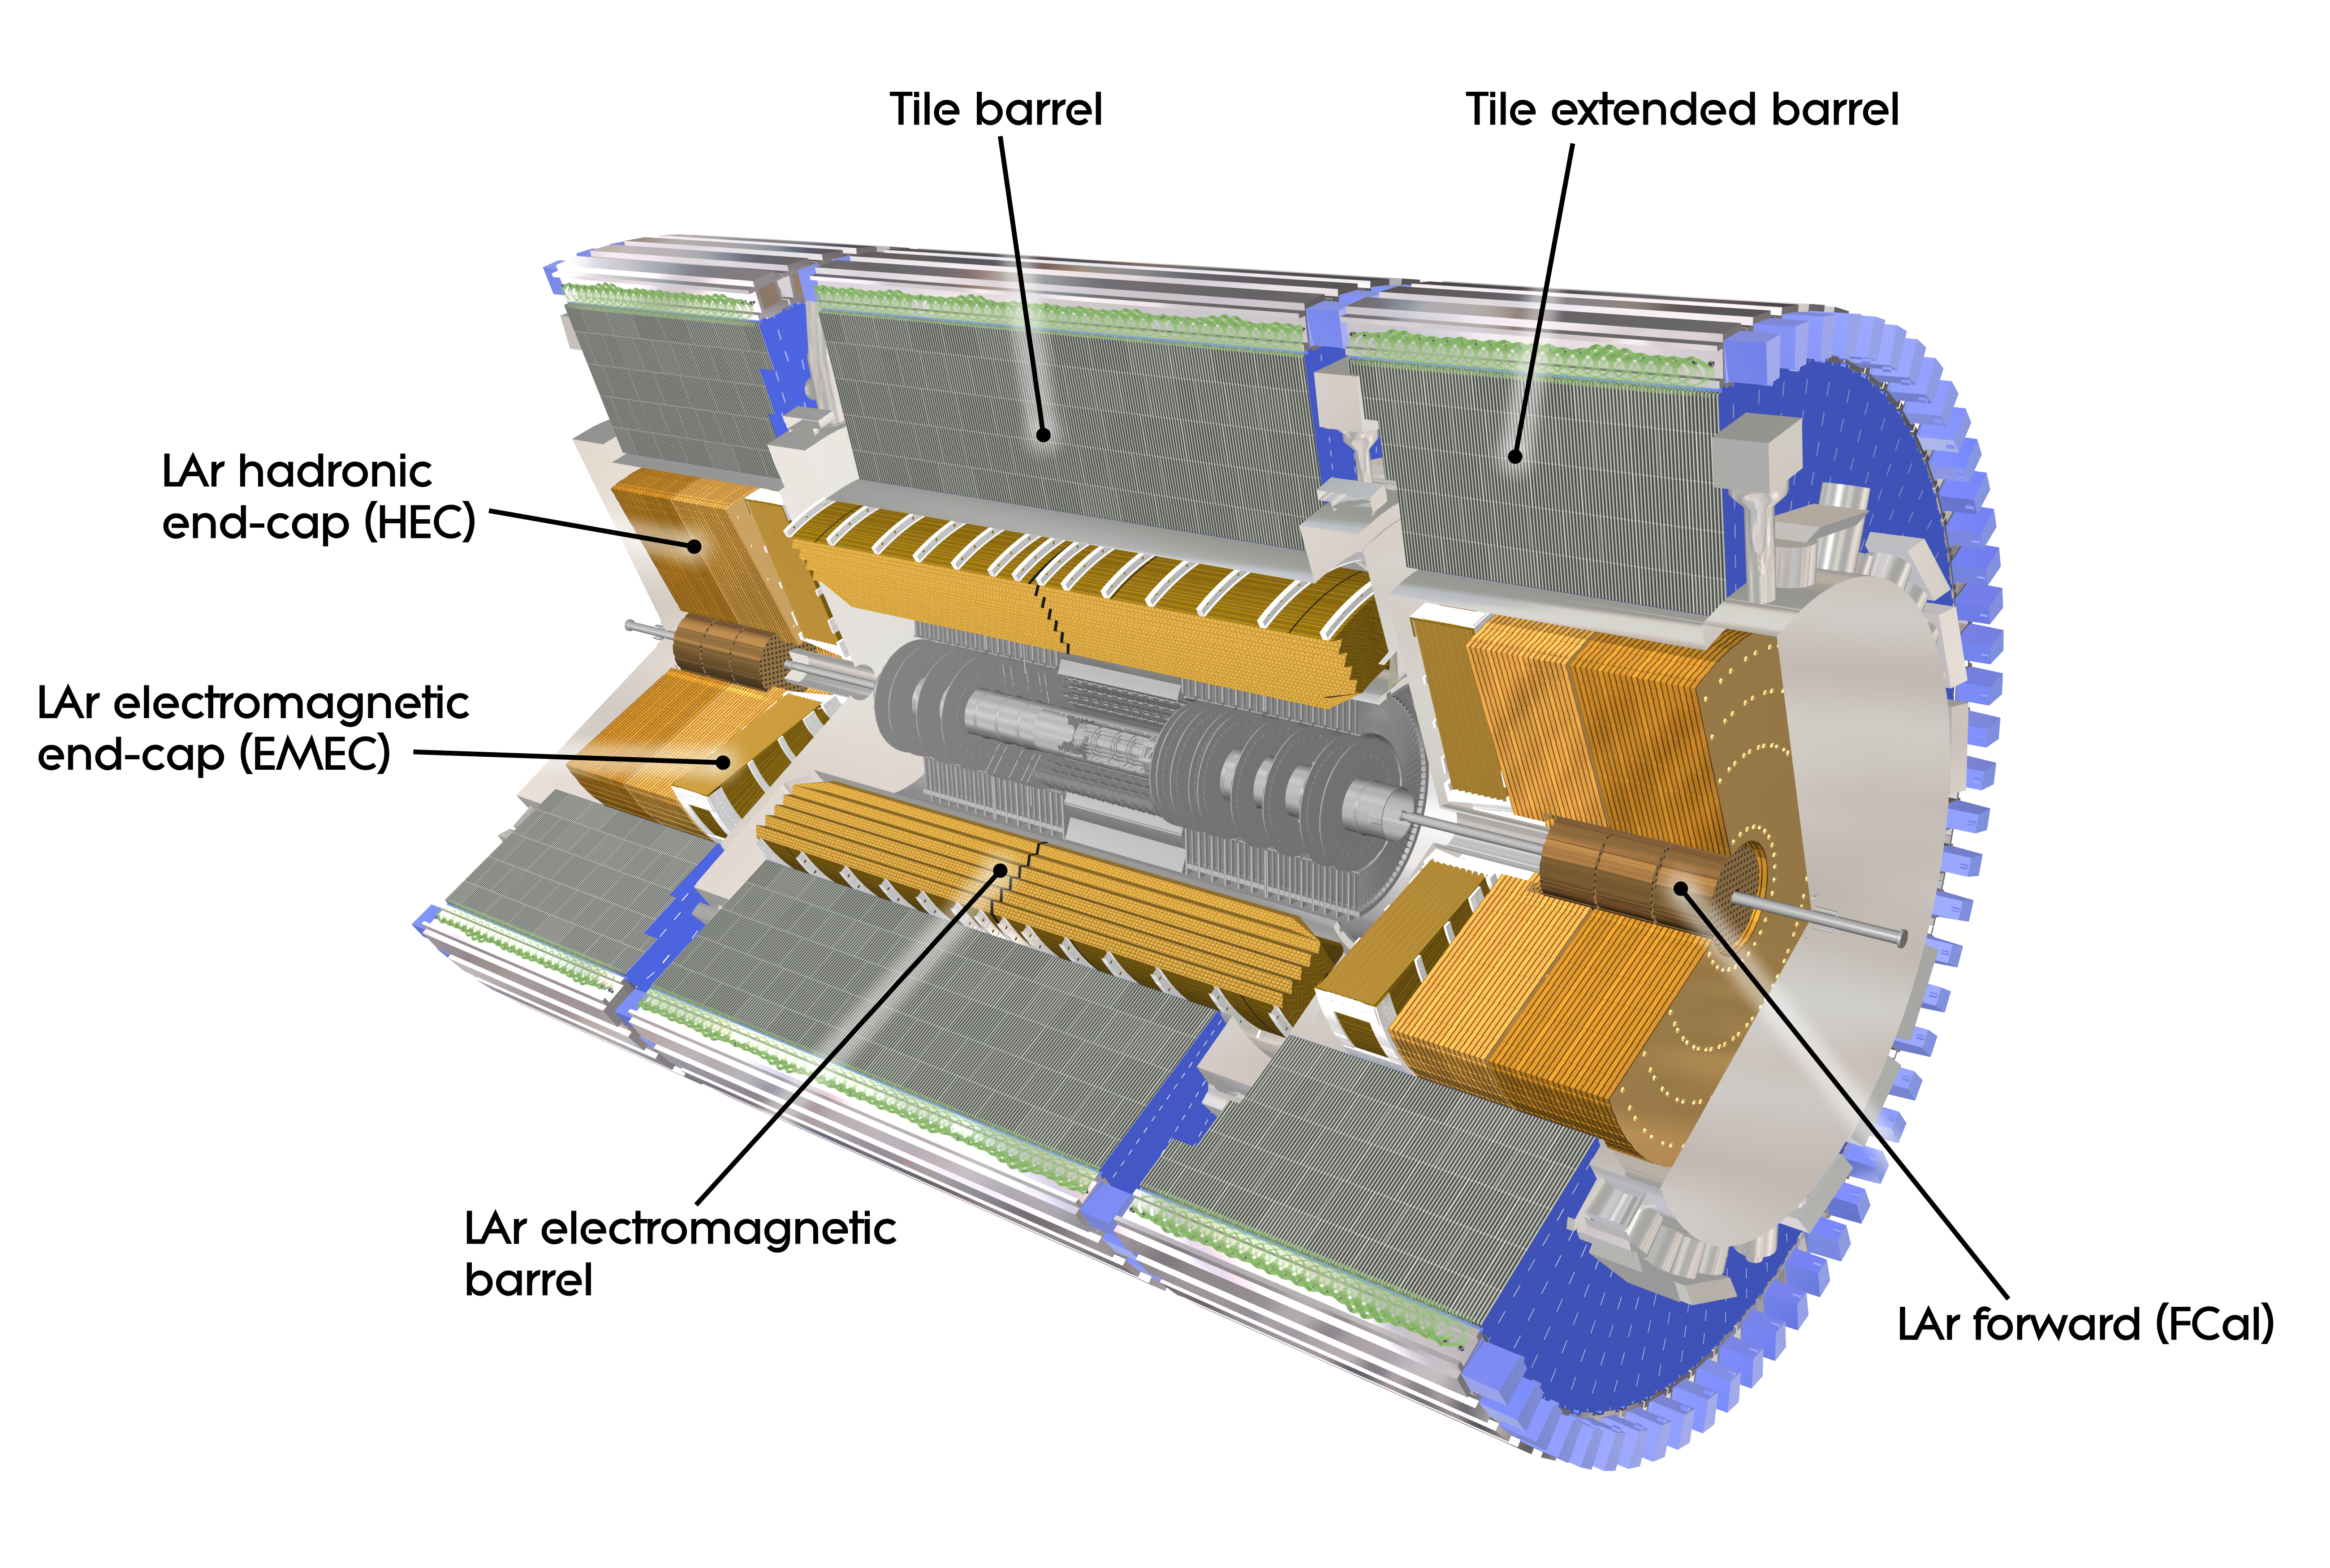
\includegraphics[width=1.0\textwidth]{Detector/ATLAS/CALO/Calo-overview_orig}
		%\setlength{\belowcaptionskip}{-20pt}
		\caption{Labelled schematics of the \ac{ATLAS} \ac{ECAL} and \ac{HCAL} system~\cite{ATLASJINST}.}
		\label{fig:calorimeters}
		\end{figure}
	The \ac{ATLAS} calorimeters are designed measure the energy of electromagnetic (\ac{ECAL}) and hadronic (\ac{HCAL}) interacting particles. 
	%The system is comprised of two main sub-detectors, the \ac{ECAL}~\cite{ATLASLAR} and \ac{HCAL}~\cite{CERN-LHCC-2017-019}, as seen by the schematics shown in Figure~\ref{fig:calorimeters}.
	The energy of electromagnetically interacting particles, such as  electrons, positrons, or photons, is measured in the \ac{ECAL}~\cite{ATLASLAR}, which is comprised of one barrel and two end-cap sensors located around the central solenoid.
	%Electromagnetically-interacting particles, such as electrons, positrons, or photons, are intercepted by the first calorimeter, comprised of one barrel and two end-cap sensors located around the central solenoid, the \ac{ECAL}. 
	The \ac{HCAL}~\cite{CERN-LHCC-2017-019} is also comprised of one barrel and two end-cap sectors and it is located around the \ac{ECAL}, so that particles travelling through the detector will have to go first go through the \ac{ECAL} and then the \ac{HCAL}. 
	It is tasked with the detection and measurement of the energy deposited by hadronic showers. 
	This is done by using tile sensors in the barrel made of scintillating plastic, while \ac{LAr} is used in the end-caps.
	Figure~\ref{fig:calorimeters} shows a detailed schematics of the calorimeter system used by the \ac{ATLAS} detector.
	More detail of the \ac{ECAL} and \ac{HCAL} geometry, functionality, and materials is given in the following paragraphs. 
	
	\begin{description}
	\item[\ac{ECAL}]
	The \ac{ECAL} utilises \ac{LAr} to measure electromagnetic showers that occur when a high-energy electron or photon travel through the fluid. 
	Photons that are above a few \mev\ will interact primarily via pair production, in which a highly energetic photon will interact with a nucleus to create a electron-positron pair. High-energy electrons and positrons, on the other hand, will produce photons via \brem. 
	These two processes will continue in the \ac{ECAL} until the energy of the emitted photons falls below the pair production threshold. At that point the energy loss of the electron will start to dominate.
	The \ac{ECAL} uses an "accordion"-geometry, shown in Figure~\ref{fig:ECAL}, comprised of multiple layers of \ac{LAr} sampler and \ac{Pb} absorber, to achieve a full $\phi$ coverage with no non-interactive regions (referred to as "cracks"), and fast extraction of signals from both front or read end of the electrodes. 
	The barrel and end-cap sectors provide a pseudorapidity coverage of up to $|\eta|<1.475$ and $1.375<|\eta|<3.20$, with the junction between the barrel and end-cap components being defined as a crack region from which any signal should be discarded. 
	An additional thin \ac{LAr} layer with no absorber is placed in front of the calorimeter in the $|\eta|<1.8$ region. 
	This layer is designed to correct for the energy lost, as particles enter the calorimeter, by taking a measurement just before the majority of the electromagnetic shower is developed. 
	\begin{figure}[!hbt]
		\centering
		\includegraphics[width=0.45\textwidth]{Detector/ATLAS/CALO/ECAL}
		%\setlength{\belowcaptionskip}{-20pt}
		\caption{Schematics of the \ac{ECAL} accordion-geometry.}
		\label{fig:ECAL}
		\end{figure}
		
	\item[\ac{HCAL}: ]
	Steel and scintillating tiles coupled with optical fibres are read out by photo-multipliers in the \ac{HCAL}.
	A central barrel, 5.64 m long covering $|\eta|<1.0$, and two extended barrels, 2.91 m long covering a region $0.8<|\eta|<1..7$ make up the \ac{HCAL}. 
	Each cylinder is composed of 64 modules, each of which is made of three layers. 
	The forward region, closest to the beam, is covered by a \ac{LAr} \ac{FCal}.
	The smallest section of the calorimeter module is a cell with a $\Delta\phi\times\Delta\eta=0.1\times0.1$ granularity for the two innermost layers and  $\Delta\phi\times\Delta\eta=0.2\times0.1$ for the outermost one.
	\end{description}
	\subsection{Muon spectrometer}
	\label{subsec:muon_spec}
	\begin{figure}[!hbt]
		\centering
		\includegraphics[width=0.9\textwidth]{Detector/ATLAS/CALO/MS}
		%\setlength{\belowcaptionskip}{-20pt}
		\caption{Computer generated schematics of the \ac{ATLAS} \ac{MS} system (taken from ~\cite{ATLASJINST}) .}
		\label{fig:muon_spectrometer}
	\end{figure}
	Muon particles are minimal interacting and are thus able to travel through the entire \ac{ATLAS} detector. 
	The \ac{MS}~\cite{MSTDR} is thus designed to accurately measure the momenta of these particles. 
	It is located within the 4 T magnetic filed generated by the long barrel toroid, described in Section~\ref{subsec:magnet}, and is comprised of three concentric chambers in the barrel region with an outer radius of 10 m, and three layers of chamber planes perpendicular to the beam pipe in the end-caps at a maximum distance of 21.5 m (as shown in Figure~\ref{fig:muon_spectrometer}). 
	High precision momentum measurements are possible by performing high precision tracking on the deflected trajectories of the charged muons as they travel through the different layers of the \ac{MS}.
	The large barrel toroid covers a region of $|\eta|<1.4$, while two end-cap toroids deflect tracks between $1.6<|\eta|<2.7$. 
	A combination of both magnets is used for the "transition" region $1.4<|\eta|<1.6$.
	Two types of chambers are used in the barrel: the \acp{MDT} and \acp{RPC}. The \acp{MDT} are also present in the end-cap layers, along with \acp{CSC} and \acp{TGC}. A more detailed description of each of the chamber systems used in the \ac{MS} is given in the following paragraphs. 
	\begin{description}
	\item[\acp{MDT}] are 29.97 mm diameter drift tubes, filled with pressurised $93\%\,\mathrm{Ar}+7\%\,\mathrm{CO}_2$ gas, employed in most of the pseudo-rapidity range to provide measurements of track coordinates in the bending direction. Electrons resulting from the ionization of the gas from a penetrating muon are collected by a tungsten-rhenium wire, measuring 50 \mum\ in diameter, located at the centre of the tube.
	Three to eight layers of drift tubes are used in both barrel and end-caps to allow a total of twenty measurements for each track. \acp{MDT} can achieve an average resolution of 80 \mum\ per tube, or about 35 \mum\ per chamber.
	\item[\acp{CSC}] are used in the innermost tracking layer for the higher particle flux and muon-track density forward direction ($2<|\eta|<2.7$), due to their higher rate capability and time resolution compared to \acp{MDT}.
	\ac{CSC} consist of two disks with eight chambers each, where each chamber contains four multi-wire proportional chambers with four cathode plates. The chambers are filled with  $80\%\mathrm{Ar}+20\%\mathrm{CO}_2$ gas, with the cathode strips aligned both parallel and perpendicular to the anode wires, to provide precision and transverse coordinates. 
	The achieved resolutions of the \ac{CSC} is 40 \mum\ in the bending plane and 5 mm in the transverse plane. 
	\item[\acp{TGC}] are very similar to \ac{CSC} and compliment the precision tracking system provided by the \ac{MDT} and \ac{CSC} by delivering track information within a few tens of nanoseconds after the passage of the particle. 
	Like \ac{CSC}, they are multiwire proportional chambers filled with $55\%\mathrm{CO_2+}$45\%n-pentane gas, with the cathode plates 2.8 mm and the anode wires 1.8 mm apart. 
	This configuration, along with high electric field, results in very good time resolutions.
	\acp{TGC} are essential for providing muon triggering and secondary complementary coordinates, orthogonal to the precision measurements, in the end-caps for the $1.05<|\eta|<2.7$ region. 
	Nine space-points are recorded for every track using a \ac{TGC}.
	\item[\acp{RPC}] are also used, like \acp{TGC}, to provide muon triggering and secondary coordinate in the barrel for $|\eta|<1.05$.
	They are parallel electrode-plate detectors, made of plastic laminate 2 mm distance apart, filled with $\mathrm{94.7\% C_2H_2F_4+5\% Iso-C_4H_{10}+0.3\% SF_6}$ gas. A maximum of six space-points are recoded for every track.
	\end{description}
	\section{The ATLAS Trigger and Data Acquisition}	
	\label{sec:ATLAStrig}
	The \ac{LHC} provides the \ac{ATLAS} experiment with $\sim$40 MHz of $pp$ collisions. 
	A sophisticated \ac{TDAQ}~\cite{TDAQRun1,TDAQRun2} system is used to reduce this rate of data down to manageable levels ($\sim$1 kHz) by storing only events that contain potentially "interesting" physics. 
	A two level trigger system has been used during Run 2, consisting of a hardware-based trigger, named \ac{L1}, and a software-based trigger, called \ac{HLT}. 
	Low granularity information from the calorimeter and muon spectrometer systems is processed by the \ac{L1} to identify so-called \acp{RoI} before making a decision. Event data from other sub-detectors and systems is stored in memory until the \ac{L1} decision is taken.
	Upon passing the rapid \ac{L1} selection, the event data is passed to the \ac{HLT} system.
	The \ac{HLT} is made of software running on computer cluster (\ac{HLT} farm), which use information not available to the \ac{L1}, such as finer-granularity calorimeter inputs and precious measurements from the \ac{MS}, to further analyse the event-data and decide whether to keep or discard the event. 
	The flow of data though the \ac{L1} and \ac{HLT} system is managed by the data acquisition system, which eventually passes all accepted events into data streams for offline physics, monitoring, and detector  analyses. 
	Objects that do not meet the \ac{L1} or \ac{HLT} requirements are discarded. 
	The \ac{ATLAS} trigger system is discussed in detail in Chapter~\ref{ch:trigger}.
	
	
  \chapter{The ATLAS Trigger System}
\label{ch:trigger}
%\epigraph{\emph{If you're serious, you can accomplish anything through diligent application of science.}}{Byakuya Ishigami - Dr Stone}
\epigraph{\emph{There are patterns I must follow, just as I must breath each breath. Like a rat in a maze, the path before me lies.}}{Simon \& Garfunkel}
%I want to be the very best, like no one ever was.} }{Ash Ketchum}
The \ac{ATLAS} inner detector trigger system together with its performance for Run 2 will be presented in this chapter. 
	A brief introduction of of motivation behind the need of a trigger system, together with its implementation in \ac{ATLAS} will be discussed.
	The \ac{L1} and \ac{HLT}) stages of the trigger will be discussed in Section ~\ref{sec:L1} and ~\ref{sec:HLT}, respectively. 
	Section ~\ref{sec:idtrigperf} will be dedicated to the description and performance of the tracking and triggering performed by the inner detector trigger system for electrons, muons taus and $b-$jet triggers. 
	The study of the performance of these triggers has been part of the author's \textit{qualification task} and the results have been collected in a paper that is currently under collaboration review.
	The study of the tau-triggers in particular are extremely important for the identification of tau discussed in Chapter ~\ref{ch:fake_est}, the analysis discussed in Chapter ~\ref{ch:analysis} and the development of future low-\pt\ threshold triggers discussed in Appendix~\ref{ch:beyondlhc}.	
	
	\section{Overview}
	\label{sec:Trig_intro}
	In 2016, 2017 and 2018 the \ac{ATLAS} detector recorded 35.6 \infb, 46.9 \infb, and 60.6 \infb\ respectively of proton-proton collision data at centre-of-mass energy of 13 \tev. 
	Due to storage and processing limitations it is not feasible  to store all the information about the collisions after every bunch crossing. 
	The ATLAS trigger system ~\cite{ATLASTrigger2015,Sutton:2695048} is thus indispensable for reducing the read-out rate without discarding potentially interesting events for the \ac{ATLAS} physics programme. 
	The trigger operates with a multi-level architecture, consisting of both hardware- and software-based real-time algorithms for the identification of interesting events. 

  The \ac{TDAQ} system is comprised of the first-level hardware-based \ac{L1} trigger, followed by the software-based \ac{HLT}.  
  Figure ~\ref{fig:TDAQ} shows schematic of the architecture structure of the \ac{TDAQ} system, including the \ac{FTK} system which, however, was being commissioned during the Run 2 data collection period and thus was not used for the results shown here. 
  The \ac{L1Calo} and \ac{L1Muon} triggers are used as inputs to the \ac{CTP}, which performs the trigger decision in real-time (online). 
  The events that pass the \ac{L1} selection are buffered in the \ac{ROS} ~\cite{Jenni:616089} so that they can be ready for distribution to a farm of the \ac{HLT} processing nodes. 
  Because of the extremely high data volume in the \ac{SCT} and Pixel detectors, these can only be read out following a L1 accept and as such the \ac{HLT} is the first stage at which tracks can be reconstructed in the silicon layers.
  The \ac{HLT} receives information on the Region of Interest (\ac{RoI}) defined by the \ac{L1} to perform the reconstruction in the trigger algorithms.. An \ac{RoI}s are extended wedge-shaped spatial regions in the detector used to reduce the amount of data (between 2\%-6\% of total volume of data ~\cite{ATLASmuontrigger}) to be transferred and processed.  
  The geometry of an \ac{RoI} in the \ac{HLT} changes between the different object candidates to be reconstructed, but it is generally constructed as a region originating from and extending along the beam-line (see section ~\ref{sec:idtrigtrack} for further details).
%\ac{L1} trigger decision is formed by the Central Trigger Processor (\ac{CTP}), which  
\begin{figure}[!hbt]
\centering
\includegraphics[width=\textwidth]{IDTrig/schematics/TDAQSystem}
\caption{The \ac{ATLAS} \ac{TDAQ} system in Run 2 with emphasis on the components relevant for triggering ~\cite{ATLASTrigger2015}. The \ac{FTK} system was being commissioned during Run 2 was thus not used for the results shown here.}
\label{fig:TDAQ}
\end{figure}  
  
  The ATLAS triggers are configured into different categories. Triggers are generally defined as \textit{trigger chains} which start from a \ac{L1} trigger and specify a sequence of reconstruction and selection steps required for the signature of interest. The naming convention is as follows: 
 $$\mathrm{TriggerLevel\_TypeAndThreshold\_Identification\_Isolation\_L1Thresholds}$$
  Where, "TriggerLevel" refers to either \ac{L1} or \ac{HLT}, "TypeAndThreshold" refers to the type of object that is being triggered (electron, muon, tau, jet, etc.) and its energy threshold.
   If any identification and/or isolation criteria are used, they are appended to the end of the \textit{trigger chain} name
    \ie: \texttt{HLT\_tau25\_medium1\_tracktwo} is a tau trigger at \ac{HLT} level with a 25 GeV threshold, using "medium" identification criteria and have between 1 and 3 tracks in the inner detector ("\textit{tracktwo}"). 
    For \ac{HLT} triggers, any additional \ac{L1} requirements are described in the "L1Thresholds" and appended to the end of the trigger chain.
   
	It is important to note that not all triggers need or are able to run at their full rate, due to the high luminosity achieved at the \ac{LHC} and abundance of trigger objects (\eg\ single jet triggers). 
	In these cases a sub-sample of events passing the trigger requirements are enough. 
	Some triggers have a thus purposefully decreased output rate, known as \textit{prescale}, which can be applied at \ac{L1} and/or at the \ac{HLT}.
	A trigger with a prescale of $N$ would indicate that the trigger accepts 1 out of $N$ events. 
	 
	\section{Level-1 Trigger}
	\label{sec:L1}
	The \ac{L1} trigger decision is performed by the \ac{CTP}, which uses the information gathered by the \ac{L1Calo} and \ac{L1Muon} trigger systems. The \ac{L1Calo} trigger ~\cite{ATLASJINST,ATLASL1CaloTrig} is based on coarse granularity data inputs from the electromagnetic and hadronic calorimeters. 
	It aims to identify high-$E_T$\ objects such as electrons and photons, jets and $\tau$-leptons decaying into hadrons as well as events with large \met\ and large total transverse energy. 
	For electron/photon and $\tau$ triggers isolation can be required. 
	Isolation implies that the energetic particle must have a minimum angular separation from any other significant energy deposit in the same trigger. 
	
	\ac{L1Muon} trigger is based on input signals from the muon trigger chambers: \ac{RPC} in the barrel and \ac{TGC} in the end-caps. The trigger searches for patterns of hits consistent with high-\pt\ muons originating from the interaction region. %The logic provides six independently programmable \pt\ thresholds.
	Muons are not double counted across the different thresholds.
	
	While the \ac{L1} trigger is based only on the multiplicity of trigger objects (or flags indicating which thresholds were passed, for global quantities), information about the geometric location of triggers objects is retained in the muon and calorimeter processors. Once the event is accepted by the \ac{L1} trigger, this information is sent as an \ac{RoI} to the \ac{HLT}.
	Due to the high rate of interactions, the latency, which is the the time taken from the proton-proton collision until the L1 trigger decision, must be kept as short as possible. The design of the trigger requires the \ac{L1} latency to be less than 2.5 $\mu$s. To achieve this aim the \ac{L1} trigger is implemented as a system of purpose-built hardware processes. The \ac{L1} trigger is thus able to reduce the peak data rate from 40 MHz (rate of collision at LHC) down to a more manageable 100 kHz. 
	\section{High-Level Trigger}
	\label{sec:HLT}
	Events that pass the \ac{L1} are buffered by the \ac{ROS} and then processed by the \ac{HLT}. The \ac{HLT} trigger is able to access information not available to the \ac{L1}, such as finer-granularity calorimeter inputs, precision measurements from the \ac{MS} and tracking information from the \ac{ID} pixel and \ac{SCT}. The information provided to the \ac{HLT} is in the form of \ac{RoI}s, which allows for faster reconstruction algorithms as the range of the detector does not need to be processed. 
	The \ac{HLT} triggers reconstruct tracks first using a fast but less accurate reconstruction algorithm, which is able to reject the majority of uninteresting events. Following this first stage a second more precise (but slower) reconstruction algorithm is run using the results of the first stage on the remaining events. Using this software based reconstruction and event acceptance algorithms the \ac{HLT} trigger system is able to reduce the peak input rate from 100 kHz, from the \ac{L1} trigger, down to 1.2 kHz. Events that are accepted by the \ac{HLT} are transfered to a local storage at the experiment site and exported to the \ac{CERN}'s computing centre for offline reconstruction ~\cite{collaboration_2020}. 
		\section{Inner detector Trigger Tracking}
		\label{sec:idtrigtrack}
		As mentioned previously, to reduce precessing time a two-step tracking approach is implemented by the \ac{HLT} triggers: the \textit{fast tracking} and the \textit{precision tracking}.
	The \textit{fast tracking} consists of a trigger specific pattern recognition, while the \textit{precision tracking} relies heavily on offline algorithms, and is seeded with the information from the \textit{fast tracking} step ~\cite{ATLASTrigger2015,ATL-DAQ-PUB-2013-002}.
	
	The tracking of electrons and muons is performed using the standard two-step approach consisting of the \textit{fast tracking} followed by the \textit{precision tracking}. The combination of these two steps is considered to be a single \textit{tracking stage}. The tracking of hadronically decaying taus and $b$-jets is, however, more complex and thus employs a multi-stage approach in order to reduce the volume of the \ac{RoI}, and the processing time that would be required if it were done in a single stage.
	%Electrons and muons tracking utilise a nominal approach, consisting of the two-step tracking mentioned previously, which is considered to be a single \textit{tracking stage}. The hadronic tau and $b$-jet tracking, however, employ a multi-stage approach in order to reduce the detector volume of the \ac{RoI}.
		\subsubsection*{Fast Tracking}
		\begin{figure}[!htb]
	\begin{center}
		\subbottom[]{
			\includegraphics[width=0.45\textwidth]{IDTrig/schematics/seeds-rphi}}\hspace{0.05\textwidth}
		\subbottom[]{
			\includegraphics[width=0.45\textwidth]{IDTrig/schematics/seeds-rz}}\hspace{0.05\textwidth}
	\end{center}	
	\caption{Schematics (a) the track seed information in radial bins and azimuthal sections and (b) tracks seed information in the \textit{r-z} plane.}
	\label{fig:schem_FTF}
	\end{figure}	 
	\noindent For the inital stage of track finding in the trigger the \ac{FTF} ~\cite{ATL-DAQ-PUB-2013-002} algorithm was developed to provide track candidates that could be use to seed the precision tracking stage. The \ac{FTF} design therefore prioritises track finding efficiency over purity. The \ac{FTF} pattern recognition is performed by searching for triplets of space-points (\textit{track seeds}) in bins or \textit{r} and sectors of $\phi$, as shown in Figure ~\ref{fig:schem_FTF}. 
	The selection of the triplet begins with the middle space-point, followed by the identification of the \textit{outer} and \textit{inner} space-points at larger and smaller radii respectively. The inner and outer pair of space-points must be compatible with the nominal interaction region along the beam line. 
	This region can be replaced by a restricted \textit{z}-region of the \ac{RoI} along the beam line as also shown by Figure \ref{fig:schem_FTF}, in the case of \ac{RoI} based tracking. 
	The triplet track parameters $\phi_0$, transverse momentum $p_T$, and transverse impact parameter at the point of closest approach to the beam line $d_0$, are estimated using a conformal transformation ~\cite{YEPES1996582}, with the transformation centre placed in the middle space-point and applying cuts on $d_0$ and $p_T$.
	
	Using the track seeds a simple track finding algorithm optimised for speed is utilised to form the initial track candidates. To remove duplicate tracks that share tracks seeds a dedicated algorithm is applied, which retains the tracks of higher quality selected by a fast $\chi^2$ fitter ~\cite{SUTTON2007761}. These preliminary tracks are then passed to the Kalman filter track fitter ~\cite{Kalman1987}. For speed the \ac{TRT} hits are not used in the \ac{FTF}.  Track candidates with too large $d_0$ value (\ie above 10 mm for muons and 4 mm for other signatures) are rejected in order to keep the contributions from fake tracks to a manageable level.
	
		\subsubsection*{Precision Tracking}
		To limit the \ac{CPU} usage the precision tracking stage applies a version of the offline tracking algorithms \cite{Cornelissen_2008,ATLAS-CONF-2010-072}, configured to run online in the trigger ~\cite{CERN-LHCC-97-016,Haywood:331064}, using the \ac{FTF} tracks as inputs. Track candidates are extended into the \ac{TRT} in an attempt to select \ac{TRT} hits at large radii to improve the track momentum resolution. Finally the final \ac{ID} track refit is performed using a more precise $\chi^2$ fitter algorithm ~\cite{chi2fit}.
		
		The rate of processing for the precision tracking is generally significantly lower than for the fast tracking.
		This allows for a more detailed handling of the detector conditions and better compensation for detector effects (\ie\ inactive sensors or calibration corrections). This results in the precision tracks being much closer in performance to the offline tracks than to the fast tracks. 
		Since the precision tracking uses the tracks and clusters identified by the fast tracking, by definition, the precision tracking efficiency cannot exceed that of the fast tracking.
		
		The overall purpose of the precision tracking is to perform a higher quality fit to improve the purity and quality of the trigger tracks identified by the first stage \ac{FTF}.
			
			\subsubsection*{Vertex Reconstruction}
		Two vertex reconstruction algorithms are used online: a histogramming based algorithm, and the offline vertex algorithm ~\cite{ferrari2007tracking,ATLAS-CONF-2012-042}. 
		Typically, trigger signatures use the offline vertex algorithm, with the exception of the $b$-jet trigger which uses both algorithms to maximise the vertex finding efficiency. 
		The simple histogramming algorithm works by histogramming the $z_0$ position for the point of closes approach to the beam line of each track and then calculates the vertex $z$ position. 
		This is done by using the mean of the bin centres weighted by the number of tracks in each bin for the group of adjacent bins within the 1 mm sliding window which contains the largest number of tracks. 
		All tracks passing some basic quality selection are used and are weighted equally. 
		The second algorithm is based on the offline vertex finder algorithm ~\cite{ATLAS-CONF-2012-042} with modifications applied for online running. 
		Both algorithms only run on tracks that have been reconstructed in the relevant \ac{RoI} of the track finding.  
		
		\subsubsection*{Multistage Tracking} 
	As mentioned previously, the fast and precision tracking algorithms run in distinct stages, but are considered to be part of a single \textit{tracking stage}, because there is only a single pass of the tracking over any specific \ac{RoI}. 
	Performing multiple passes of aspects of the tracking is referred as \textit{multistage} tracking. Multistage tracking can run multiple aspects of the tracking in different steps, updating the constructed \ac{RoI} at each step.
	
	The generic structure of the multistage tracking is illustrated in Figure ~\ref{fig:multi_stage} where in a region of the detector the first stage fast tracking is performed over an \ac{RoI} to identify the event vertex.
	 Given the results of the first stage the dimensions of the \ac{RoI} are changed into a different \ac{RoI}. 
	  The second stage executes the fast tracking again, followed by the precision tracking for the tracks found in this second fast tracking stage, run in this new \ac{RoI}. This process is trigger specific and will be discussed in more details for the relevant object below.
	%\begin{wrapfigure}{R}{.45\textwidth}
	\begin{figure}[!hbt]
	\centering
	\includegraphics[height=0.55\textheight]{IDTrig/schematics/multi-stage}
	\caption{Schematics illustrating multistage tracking. And initial first stage is fast tracking performed on an \ac{RoI}, followed second fast and precision tracking stages run over a second stage \ac{RoI}.}
	\label{fig:multi_stage}
	\end{figure} 
%\end{wrapfigure}

	Hadronic tau triggers require a larger \ac{RoI} than for instance, electrons, to allow for the opening angle of the tracks from the three prong decay. To limit the tracking \ac{CPU} usage in this wider \ac{RoI} a mutlistage approach us used, as illustrated by Figure ~\ref{fig:roi_tau}. 
	In the first stage the fast tracking is run to identify the position of tau event vertex and leading track along the beam line in a narrow \ac{RoI} with a full width of 0.2 in both $\eta$ and $\phi$, but fully extended along the beam line in the range of $|z|<$ 225 mm, represented by the purple area in the diagram. The \ac{RoI} is then changed to a wider version with full width 0.8 in both $\eta$ and $\phi$, centred on the $z$ position of the leading track identified by the first stage (as shown by the blue area on the diagram) and limited to $|\Delta z|<$ 10 mm with respect to the leading track. The fast tracking is performed in this wider \ac{RoI}, followed by the precision tracking for the tracks found in this second fast tracking stage. Even though the multistage tracking runs the tracking algorithms repeatedly for the two stages, the combined tracking volume of the first and second stage is still significantly smaller than for the \ac{RoI} in the single-stage tracking scheme. 
	\begin{figure}[!hbt]
	\centering
	\includegraphics[width=\textwidth]{IDTrig/schematics/roi-tau}
	\caption{Schematics illustrating the \ac{RoI}s from the single-stage and two-stage tau lepton trigger tracking shown in plan view, ($x-z$ plane) along the transverse direction, and in perspective view, with the $z$-axis along the beam line. The combined volume of the first and second stages of the two-stage tracking approach (blue and purple areas respectively) is noticeably smaller than the \ac{RoI} in the single-stage (pink area) tracking scheme.}
	\label{fig:roi_tau}
	\end{figure} 

The multistage approach reduces the mean processing time for the hadronic tau trigger fast tracking from 66.2 $\pm$ 0.34 ms for the single-stage, down to 23.1 $\pm$ 0.11 ms and 21.4 $\pm$ 0.09 ms for the first and second stages of the multistage approach, respectively. For the precision tracking the mean processing time was reduced from 12.0 $\pm$ 0.07 ms for the single-stage down to 4.8 $\pm$ 0.04 ms using the multistage ~\cite{Sutton:2695048}.

	A similar multistage tracking strategy is adopted for the $b$-jet trigger. In the first stage the vertex tracking is used to identify the likely event vertex $z$ position for use in the second stage for jets identified by the jet trigger with transverse energy $E_T\,>\,30$ GeV. 
	For the second stage, separate \ac{RoI}s about each jet, specialised more tightly at the beam line about the $z$ vertex position identified in the first stage, are used. 
	The tracks are then reconstructed with the fast tracking algorithm in a narrow region with full width of 0.1 in $\eta$ and $\phi$ around the jet axis of each jet, but with $|z|\,<$ 225 mm along the beam line.
	 To prevent multiple processing of overlapping regions of the detector, before running the fast tracking, the \ac{RoI}s about each jet axis are aggregated into a \textit{super \ac{RoI}}, as shown by Figure ~\ref{fig:superroi}.
	  This super  \ac{RoI} is used to determine which detector elements should be read out by the data preparation stage.
	
	Following this stage the tracks identified in the super \ac{RoI} are used for the primary vertex reconstruction ~\cite{Meloni_2016}. This vertex is used to define wider \ac{RoI}s with $|\Delta\eta|$ and $|\Delta\phi|$ less then 0.4 each, with respect to the jets axis, but with $|\Delta z|\,<$ 10 mm relative to the primary vertex $z$ position.
	These \ac{RoI}s are used for the second-stage reconstruction which runs the fast tracking in a wider $\eta$ and $\phi$ regions about the jets. The precision tracking, primary vertexing and $b$-tagging algorithms are all subsequently run. As in the case of the tau multistage tracking, the use of this multistage process reduces significantly the mean processing time. 
	\begin{figure}[!hbt]
	\centering
	\includegraphics[width=\textwidth]{IDTrig/schematics/superroi}
	\caption{A schematic illustrating the creation of the super \ac{RoI} from all the trigger jets reconstructed with an $E_T\,>$ 30 GeV.}
	\label{fig:superroi}
\end{figure} 

	
	\section{ID tracking Performance}
	\label{sec:idtrigperf}
	The performance of muon and electron triggers is presented for the full available luminosity for the 2016-2018 data collection period, collected at the \ac{ATLAS} experiment using 13 TeV $pp$ collision events. This was possible since the processing for these triggers did not change significantly throughout data taking. For the tau and $b$-jet signatures, which ran multistage tracking, significant changes were made to the reconstruction of either the first or second stages of the multistage process over the data collection period. These changes include the modification to the second stage seed finding. Therefore only results for 2018 are  presented in full details for these signatures. 
	
	To remain as unbiased as possible, specific monitoring triggers that do not require a track to be present for the event to be accepted are used for the estimation of efficiency of the tracking. 
	The efficiency, residuals and resolutions presented below are calculated with respect to the tracks found by the offline reconstruction software ~\cite{Cornelissen_2008}. The efficiency is therefore defined as the fraction of offline reference tracks that are matched to a trigger track
%mathscr
	\begin{equation}
	\pazocal{F}\,=\,\frac{\mathrm{N_{trigger}}}{\mathrm{N_{offline}}},
	\end{equation}
	where $\mathrm{N_{trigger}}$ is the number of tracks matched to a trigger and $\mathrm{N_{offline}}$ is the number of tracks reconstructed by the offline reconstruction software.
	For any given offline track, the reconstructed track that matches the closest to a loose preselection cone of size $\Delta R\,=\,\sqrt{(\Delta\eta)^2+(\Delta\phi)^2}\,=\,0.05$ to the offline track, is chosen as a match. 
	%The reconstructed tracks are considered matched to an offline track if they are 
		\subsection*{Muon trigger}
		Figure ~\ref{fig:muon_idtrig_perf} shows the tracking efficiency for medium quality ~\cite{cite-key} offline muon candidates, using a range of HLT triggers ~\cite{ATLAS-CONF-2012-099} to cover the whole transverse momentum reconstruction spectrum down to 4 \gev, for the fast and precision tracking.  
		Two representative thresholds are used for the offline muon selection: $p_T\,>$ 4 \gev\ corresponding to the lowest trigger threshold, and $p_T\,>$ 20 \gev for the higher trigger thresholds. 
		The efficiency shown for both the fast and precision tracking is significantly better than 99\% and flat as a function of pile-up interaction multiplicity. The small apparent loss in precision tracking for higher \pt\ tracks is primarily caused by the offline reconstruction. Poorly reconstructed candidates of lower \pt\ are occasionally mis-reconstructed at higher momentum by the offline reconstruction, thus creating a larger expected contribution in the reference sample in the high \pt\ region. Therefore poorly offline reconstructed low \pt\ tracks cause the apparent loss in efficiency at higher \pt. It is therefore not an inefficiency that derived from the online \ac{ID} triggers.
		\begin{figure}[!htb]
	\begin{center}
		\subbottom[]{
			\includegraphics[width=0.45\textwidth]{IDTrig/performance/muon/HLT_pT_eff}}\hspace{0.05\textwidth}
		\subbottom[]{
			\includegraphics[width=0.45\textwidth]{IDTrig/performance/muon/HLT_eff_vs_muRebin2}}\hspace{0.05\textwidth}
	\end{center}	
	\caption{\ac{ID} trigger efficiency as a function of (a) the offline reconstructed muon \pt, (b) the mean pile-up interaction $<\mu>$ for muons selected by 4 GeV and 20 GeV muon support triggers with respect to medium offline muon candidates with \pt\ $>$ 4 GeV or \pt\ $>$ 20 GeV.}
	\label{fig:muon_idtrig_perf}
	\end{figure}	 
	
	The resolutions for the trigger tracks in $\eta$ and $d_0$ with respect to the offline muon candidate pseudorapidity and \pt\ are shown in Figure ~\ref{fig:muon_idtrig_res}. The fast and precision tracking $d_0$ resolutions are found to be better than 25 $\mu$m and 20 $\mu$m respectively, for muons candidates with offline \pt\ $>$ 4 GeV. The difference in resolution between the two algorithms is due to the fact that the precision tracking performs a higher quality fit using the space points identified by the fast tracking, which improves the purity and quality of the trigger tracks. The degrade of resolution observed at larger pseudorapidities is predominantly due to the increased amount of material through which tracks must travel. The position of the endcap silicon detectors (perpendicular to the beam line) partially ameliorate this, the effect of which can be seen for presudorapidities larger than 1.2 which is the approximate boundary between the barrel and endcap silicon detectors.
		\begin{figure}[!htb]
	\begin{center}
		\subbottom[]{
			\includegraphics[width=0.45\textwidth]{IDTrig/performance/muon/HLT_rd0_vs_pt_sigma}}\hspace{0.05\textwidth}
			\subbottom[]{
			\includegraphics[width=0.45\textwidth]{IDTrig/performance/muon/HLT_reta_vs_eta_sigma}}\hspace{0.05\textwidth}
	\end{center}	
	\caption{\ac{ID} trigger track resolution for (a) transverse impact parameter with respect to the beam line ($d_0$) and (b) pseudorapidity ($\eta$) as a function of offline muon $\eta$ and \pt\ for muons selected by 4 GeV and 20 GeV muon support triggers with respect to medium offline muon candidates with \pt\ $>$ 4 GeV or \pt\ $>$ 20 GeV.}
	\label{fig:muon_idtrig_res}
	\end{figure}	
	
		\subsection*{Electron trigger}
		
		Offline electron candidates are reguired to pass the tight identification criteria ~\cite{Aaboud_2019}, have at least two pixel hits, an \ac{IBL} hit if passing through at least one active \ac{IBL} module, and at least four clusters in the \ac{SCT}. These requirements have been selected to eliminate poorly reconstructed Brehmsstrahlung candidates and insure better reconstruction in the pixel detector.
		 A range of \ac{HLT} triggers is used to cover the whole transverse momentum reconstruction spectrum down to 5 \gev\ (and $|\eta|\,<$ 2.5), for the offline electron candidate tracks. 
		 For the candidates from the 5 \gev, 10 \gev\ and 26 \gev\ triggers a selection of $E_T\,>$ 5 \gev, $E_T\,>$ 10 \gev\  and $E_T\,>$ 26 \gev\ was applied, respectively. However for all three triggers the same 5 \gev\ track \pt\ selection was requested. 
		Offline candidates with $E_T/p_T\,<$ 0.8 are been removed (except for the $E_T/p_T$ plot in Figure ~\ref{fig:electron_idtrig_eff_c}), where the $E_T$ is measured in the calorimeter and $p_T$ from the track. This is done to remove offline candidates where the track \pt\ has been badly overestimated.
		% To remove offline candidates where the track \pt\ has been badly overestimated, offline candidates with $E_T/p_T\,<$ 0.8 have been removed (with the exception for the $E_T/p_T$ plot), with $E_T$ is measured in the calorimeter and $p_T$ from the track.
		
	\begin{figure}[!htb]
	\begin{center}
		\subbottom[]{
			\includegraphics[width=0.45\textwidth]{IDTrig/performance/electron/HLT_eff_vs_ET}\label{fig:electron_idtrig_eff_a}}\hspace{0.05\textwidth}
			\subbottom[]{
			\includegraphics[width=0.45\textwidth]{IDTrig/performance/electron/HLT_pT_eff}\label{fig:electron_idtrig_eff_b}}\hspace{0.05\textwidth}
			\subbottom[]{
			\includegraphics[width=0.45\textwidth]{IDTrig/performance/electron/HLT_eff_vs_etovptrebin26}\label{fig:electron_idtrig_eff_c}}\hspace{0.05\textwidth}
	\end{center}	
	\caption{\ac{ID} trigger efficiency as a function of (a) the offline reconstructed electron $E_T$, (b) the offline reconstructed electron track \pt, and (c) offline electron $E_T/p_T$ for electrons selected by 5 GeV and 26 GeV muon support triggers with respect to medium offline muon candidates with \pt\ $>$ 5 GeV or \pt\ $>$ 26 GeV. For the efficiency }
	\label{fig:electron_idtrig_eff}
	\end{figure}	
	Figure ~\ref{fig:electron_idtrig_eff} shows the \ac{ID} track efficiency for the 5 \gev\ and 26 \gev\ electron triggers as a function of offline electron \pt\ and $E_T$. The efficiencies for the fast and precision track finder are consistently high and exceed 99\% for all values of $E_T$. For tracks candidates from the 26 \gev\ trigger with \pt\ below 26 \gev, there is significant radiation, which may cause "kinks"  in the electron trajectory and thus decrease in the track reconstruction efficiency. Nonetheless, even for this case, the efficiency exceeds 97\%  in the low \pt\ range and reaching above 99\% at ~20 GeV.
	 For Figure ~\ref{fig:electron_idtrig_eff_c} the $E_T/p_T$ selection has been relaxed. Here, the long tail values greater than unity represent the \brem\ candidates which have radiated energy away into the calorimeter, and thus have an $E_T$ value that is greater than the track \pt. 
	 The contribution of \brem\ differs when selecting different offline $E_T$ values. For the 5 GeV trigger the \brem\ will be less then for the 26 GeV trigger. 
	Values with $E_T/p_T$ below unity represent electron candidates that have a track \pt\ that is larger than the calorimeter cluster $E_T$. This is a consequence of offline low \pt\ tracks being misreconstructed with larger values. These tracks can not have significantly more energy than the cluster, and therefore represent less reliable track \pt\ measurements. 
	There is a clear reduction in the $E_T/p_T$  efficiency for values below unity, but with only 1\% reduction for tracks where the track \pt\ is 60\% higher than might be physically possible. Tracks that have not radiated have an efficiency well over 99\%, while the efficiency for tracks that have radiated over half of their original energy is still greater than 98\%.
	
	\begin{figure}[!hbt]
	\begin{center}
		\subbottom[]{
			\includegraphics[width=0.45\textwidth]{IDTrig/performance/electron/HLT_reta_vs_eta_sigma}}\hspace{0.05\textwidth}
			\subbottom[]{
			\includegraphics[width=0.45\textwidth]{IDTrig/performance/electron/HLT_ript_vs_pt_sigma}}\hspace{0.05\textwidth}
	\end{center}	
	\caption{\ac{ID} trigger track resolution for (a) track pseudorapidity ($\eta$) and (b) track 1/\pt\ as a function of offline electron $\eta$ and \pt\ for electrons selected by 5 GeV and 26 GeV electron support triggers with respect to tight offline electron candidates with \pt\ $>$ 5 GeV or \pt\ $>$ 26 GeV for both the fast and precision tracking algorithms.}
	\label{fig:electron_idtrig_res}
	\end{figure}	
	
	Figure ~\ref{fig:electron_idtrig_res} shows the resolutions for the track pseudorapidity and 1/\pt\ with respect to the $\eta$ and \pt\ of the offline track from the offline electron candidate. Unlike for the events with the 26 GeV selection, events with the 5 GeV selection have no phase space for the electron candidate near the threshold to radiate any \brem\ photons. 
	As such, tracks with \pt\ below 26 GeV from the 26 GeV trigger will correspond to electrons that have undergone a significant amount of radiation. Because of this, the resolution of these tracks will be significantly worse than for the tracks with the same \pt\ but from the 5 GeV trigger. 
	As expected, the resolutions also degrades at larger $\eta$ for both the higher and lower threshold triggers in both the fast and precision tracking. Despite the worse resolution at low \pt\ for the tracks from the 26 GeV trigger, when integrated over \pt\, the resolution is significantly better than for the lower \pt\ threshold since only a relatively small fraction of events from the 26 GeV trigger will have low \pt\ tracks. 
		\subsection*{Tau trigger}
	\noindent Figure ~\ref{fig:tau_idtrig_eff} shows the efficiency for the tau tracking with respect to the offline tracking for the offline tracks with \pt\ $>$ 1 GeV originating from decays of offline tau lepton candidates with \pt\ $>$ 25 GeV.		
		For the ID trigger tracking a multistage processes was used, as described in Section ~\ref{sec:idtrigtrack}, where the first stage runs the \ac{FTF} in a narrow \ac{RoI} in $\eta-\phi$. In this narrow $\phi$ region low-\pt\ tracks (around or below 5 GeV) may bend significantly in the solenoid magnetic field. If these tracks are on or near the edge of the \ac{RoI}, they may bend outside the region and thus are not reconstructed. 
		\begin{figure}[!htb]
	\begin{center}
		\subbottom[]{
			\includegraphics[width=0.45\textwidth]{IDTrig/performance/tau/HLT_eta_eff}}\hspace{0.03\textwidth}
			\subbottom[]{
			\includegraphics[width=0.45\textwidth]{IDTrig/performance/tau/HLT_pT_eff}}\hspace{0.03\textwidth}
	\end{center}	
	\caption{\ac{ID} trigger efficiency as a function of (a) the offline reconstructed tau $\eta$ comparing performance between 2016, 2017, and 2018, and (b) the offline reconstructed tau track \pt\ for the first stage fast tracking and second stage fast and precision tracking. The efficiency is evaluated for the 25 \gev\ tau performance trigger, which does not use any ID tracking information for the selection. Only tracks from tau decays with \pt $>$ 1 \gev\ are used. Bayesian uncertainties are shown.}
	\label{fig:tau_idtrig_eff}
	\end{figure}	
	
		Figure ~\ref{fig:tau_idtrig_eff}(b) shows the efficiency for the first stage fast tracking, and for the second stage fast and precision tracking from the data collected in 2018. Due to the \ac{RoI} containment issue for low \pt\ tracks  just described above, there are fewer sample of tracks near the threshold.
		This results in lower efficiencies and larger uncertainties for both the fast and precision tracking, but more significantly for the first stage fast tracking due to the narrower \ac{RoI} used in the initial stage. 
		Efficiencies are nonetheless very high, well above 96.5\% everywhere for all fast and precision tracking in first and second stage of multistage tracking and above 99\% for second stage precision tracking for tracks with \pt\ $>$ 1.2 GeV. 
		The effect of the changes to the trigger between 2016, 2017 and 2018 can be seen for the second stage fast tracking in Figure ~\ref{fig:tau_idtrig_eff}(a). In 2016 a small inefficiency was observed at large pseudorapidities because of the tightening of the second stage \ac{RoI} about the $z-$position of the leading track. 
		Approximations used in the layer positions for the seed finding were particularly affected by the worse resolution for seeds at large $\eta$, causing a significant fraction of the seeds to be rejected. The increased rate due from the higher pile-up occupancy in 2017 required some additional changes to the seed finding used for the \ac{FTF} tracking, which resulted in the further inefficiencies observed at larger $\eta$, leaving the efficiency at central $\eta$ unaffected.
		Modifications to take into account the worse seed resolution at large pseudorapidities were under development, but were not ready for the start of data taking in 2017. For 2018 the seed finding was reimplemented which restored the efficiency at large $\eta$.
		
		\begin{figure}[!hbt]
	\begin{center}
		\subbottom[]{
			\includegraphics[width=0.45\textwidth]{IDTrig/performance/tau/HLT_rd0_vs_eta_sigma}}\hspace{0.03\textwidth}
			\subbottom[]{
			\includegraphics[width=0.45\textwidth]{IDTrig/performance/tau/HLT_rd0_vs_pt_sigma}}\hspace{0.03\textwidth}
	\end{center}	
	\caption{\ac{ID} trigger track resolution for transverse impact parameter ($d_0$) as a function of offline tau track (a) pseudorapidity $\eta$ and (b) transverse momentum (\pt), respectively.}
	\label{fig:tau_idtrig_res}
	\end{figure}	
	Figure ~\ref{fig:tau_idtrig_res} shows the resolutions for $d_0$ with respect to offline track $\eta$ and \pt. 
	As expected, the precision tracking resolution is found to be generally better than the fast tracking resolution. The fast tracking resolution is found to be vert similar between the first and second stage for tracks with offline track \pt\ $>$ 5 GeV but different for \pt\ $<$ 5 GeV. This is again due to the \ac{RoI} containment requirement discussed above. When integrating over \pt, the resolution is between 15-20 $\mu$m for all pseudorapidities. 
		\subsection*{\textit{b}-jet trigger}
		The efficiency for the tracking as a function of pile-up interactions \mubar\ from both stages of the \textit{b}-jet multistage tracking process is shown in Figure ~\ref{fig:bjet_idtrig_eff}(a), while \ref{fig:bjet_idtrig_eff}(b) compares the precision and fast tracking efficiencies as a function of offline track \pt\ for the jet tracking from the 55 \gev\ and 150 \gev\ threshold triggers. For the vertex finding only tracks with \pt\ $>$ 5 \gev\ are reconstructed and thus only offline tracks with \pt\ above 5 \gev\ have been selected. For offline tracks above ~1.2 \gev\ the second stage fast tracking efficiency is better than 99.5\% for both 55 \gev\ and 150 \gev\ threshold triggers. For tracks near 1 \gev\ the fast tracking efficiency is better than 98\% but the precision tracking efficiency is approximately 85\%\footnote{This is not shown on figure as it would extend the axis range making more relevant features of the distributions more difficult to discern.}. This is a consequence of placing a 1 \gev\ cut on tracks from the precision tracking in teh \textit{b}-jet signature for processing latency reasons. The small drop in efficiency with increasing \mubar, which is more significant for the precision tracking, is driven largely by the lower efficiencies at low \pt.  
		\begin{figure}[!htb]
	\begin{center}
		\subbottom[]{
			\includegraphics[width=0.45\textwidth]{IDTrig/performance/bjet/HLT_eff_vs_murebin2}}\hspace{0.03\textwidth}
			\subbottom[]{
			\includegraphics[width=0.45\textwidth]{IDTrig/performance/bjet/HLT_pT_eff}}\hspace{0.03\textwidth}
	\end{center}	
	\caption{\ac{ID} trigger efficiency as a function of (a) the mean pileup interaction multiplicity \mubar, comparing the \ac{RoI} based jet tracking with vertex tracking and (b) the offline reconstructed jet track \pt\ for the second stage fast and precision tracking, evaluated for the 55 \gev\ and 150 \gev\ \textit{b}-jet triggers. Bayesian uncertainties are shown.}
	\label{fig:bjet_idtrig_eff}
	\end{figure}	
	
	Figure ~\ref{fig:bjet_idtrig_res} shows the \ac{ID} trigger track $d_0$ resolutions as a function of $\eta$ and offline track \pt\ from the fast and precision tracking from the second stage of the \textit{b}-jet trigger for the 55 \gev\ and 150 \gev\ signatures.  As expected the precision tracking provides significantly better resolutions for the whole $\eta$ range and for $d_0$ values at lower track \pt. However, there is also a slight degradation of the $d_0$ resolution with increasing \pt\ for the high $E_T$ jet trigger. This is correlated with a slight loss of pixel pixel hits and thus corresponds to a loss in efficiency for the precision tracking at higher \pt, as found in figure ~\ref{fig:bjet_idtrig_eff}. When integrating over \pt, the resolution for the \textit{b}-jet \ac{ID} trigger second stange precision tracking is between 20-30 (20-35) $\mu$m for the 50 (150) \gev\ trigger.
	\begin{figure}[!hbt]
	\begin{center}
		\subbottom[]{
			\includegraphics[width=0.45\textwidth]{IDTrig/performance/bjet/HLT_rd0_vs_eta_sigma}}\hspace{0.03\textwidth}
			\subbottom[]{
			\includegraphics[width=0.45\textwidth]{IDTrig/performance/bjet/HLT_rd0_vs_pt_sigma}}\hspace{0.03\textwidth}
	\end{center}	
	\caption{\ac{ID} \textit{b}-jet trigger track resolution for transverse impact parameter ($d_0$) as a function of offline \textit{b}-jet track (a) pseudorapidity and (b) transverse momentum.}
	\label{fig:bjet_idtrig_res}
	\end{figure}	
	
		\subsection*{Vertex Finding}
		%The more robust but less accurate histogramming vertex algorithm is used for the online vertex selection to identify vertex candidates for those events where the offline based vertex algorithm failed to find a vertex. 
		For the measurement of performance, the online vertex efficiency is calculated for the single offline vertex candidate from the bunch crossings with the highest sum of the squared transverse momenta. 
		Figure ~\ref{fig:vertex_idtrig_eff} shows the efficiency for identifying the vertex candidates in the trigger for the 110 \gev\ and 420 \gev\ triggers, as a function of the offline track multiplicity in the super \ac{RoI} and the mean pile-up interaction multiplicity of the event.
\begin{figure}[!htb]
	\begin{center}
		\subbottom[]{
			\includegraphics[width=0.45\textwidth]{IDTrig/performance/vertex/HLT_ntrax_eff}}\hspace{0.03\textwidth}
			\subbottom[]{
			\includegraphics[width=0.45\textwidth]{IDTrig/performance/vertex/HLT_mu_eff}}\hspace{0.03\textwidth}
	\end{center}	
	\caption{The vertex algorithm \ac{ID} trigger efficiencies for 110 \gev\ and 420 \gev\ $E_T$ threshold \textit{b}-jet triggers. The efficiencies versus (a) the offline track multiplicity for tracks in the super \ac{RoI}, and (b) the mean pile-up interaction multiplicity are shown. Bayesian uncertainties are shown.}
	\label{fig:vertex_idtrig_eff}
	\end{figure}	
		
	A steep rising edge is found for the vertex finding algorithms with increasing offline track multiplicity. For the histogram based algorithm full efficiency is reached for event with more than four vertex tracks within the \ac{RoI}, while for the offline based algorithm full efficiency is reached only for events with more than eight 	vertex tracks.
	This is due to the tighter track quality required by the offline based algorithm. Due to this higher track quality requirement, some vertices with only a few tracks in the super \ac{RoI} may not have any tracks remaining with which to form a vertex once the tracks with lower quality are removed. 
	Higher $E_T$ jet triggers will have significantly higher tracks multiplicities and larger average tracks \pt\, making the probability of the track multiplicity for a pile-up vertex matching or exceeding that for the interaction of interest significantly lower. Both algorithms show a reduction in the efficiency as \mubar\ increases. This is due to the increased possibility of for offline selection to misidentify the jet vertex candidate within the super \ac{RoI}. Therefore, as the pile-up interaction multiplicity increases within an event, so do the chances of there being additional tracks from additional vertices within the super \ac{RoI}.
	 The lower overall efficiency of the offline based algorithm, particularly for the lower $E_T$ threshold trigger, is due to the lower overall track multiplicity in the events passing the trigger. The trigger is therefore still on the rising edge of the efficiency distribution for many events, causing a lower overall efficiency as a function of \mubar. For the higher $E_T$ thresholds triggers, the multiplicity is higher and thus the algorithm is further along the efficiency curve for most events, resulting in a higher overall efficiency. 
		\begin{figure}[!hbt]
	\begin{center}
		\subbottom[]{
			\includegraphics[width=0.45\textwidth]{IDTrig/performance/vertex/HLT_rdz_vs_ntrax_sigma}}\hspace{0.03\textwidth}
			\subbottom[]{
			\includegraphics[width=0.45\textwidth]{IDTrig/performance/vertex/HLT_rdz_vs_zed_sigma}}\hspace{0.03\textwidth}
	\end{center}	
	\caption{\ac{ID} vertex reconstruction vertex  $z$  position track resolution for 110 \gev\ and 420 \gev\ \textit{b}-jet triggers as a function of (a) the offline track multiplicity and (b) the offline $z$ vertex position.}
	\label{fig:vertex_idtrig_res}
	\end{figure}		

	The resolution of the vertex $z$ for both online algorithms as a function of the offline track multiplicity and the offline  $z$  vertex positions is shown in Figure ~\ref{fig:vertex_idtrig_res}.
	The resolution on the vertex  $z$  position for both online algorithms improves with increasing track multiplicity, with the offline based algorithm showing a significantly better resolution. The resolution of both algorithms improves logarithmically with increasing track multiplicity from 100 $\mu$m and 70 $\mu$m at low track multiplicity, to 30 $\mu$m and 20 $\mu$m at 50 tracks, for the histogram and offline based algorithms respectively. The higher resolution observed for the high $E_T$ threshold trigger is due to the larger average \pt\ of tracks from the higher $E_T$ jet triggers, such that the track  $z$  positions themselves have an intrinsically better  $z$  resolution.
	The resolution as a function of vertex  $z$  position is largely constant with a small degradation at around  $z$  mm, and a slight trend towards better resolutions for more negative  $z$  for the lower $E_T$ threshold triggers. This is especially evident for the histogram based algorithm.
	
	
	\section{Summary}
	This chapter presented the \ac{ATLAS} trigger with particular interest in the \ac{ID} trigger and tracking algorithms and corresponding performance. 
	The performance in terms of efficiency with respect to the offline algorithms, and resolutions of the \ac{ID} tracking algorithms for the main physics signatures needed by the \ac{ATLAS} physics program: muon, electron, tau, and b-jet, are shown. 
	The performance has been excellent event at the very high interaction multiplicities observed at the end of data taking in 2018. The results have been submitted for publication to \color{red} ADD JOURNAL ONCE PUBLISHED \color{black} and have been presented by the author at many conferences, including at: the Large Hadron Collider Physics conference in 2018, The Institute of Electrical and Electronics Engineers Realtime Conference in 2018, and the International Conference on High Energy Physics in 2020.
	The study of the performance of these triggers has been part of the \textit{qualification task}\footnote{To become an \ac{ATLAS} author active \ac{ATLAS} researchers must spend 50\% of their time on a technical task (for the first year) and 30\% the following year.}
	of the author.
	The excellent performance of the \ac{ID} trigger algorithms demonstrates how the \ac{ID} trigger continues to lie at the heart of the trigger performance and plays an essential r$\mathrm{\hat{o}}$le in the \ac{ATLAS} physics programme.
  \newcommand{\FeynmanDiagramStau}{
\begin{figure}[!hbt]
\centering
\includegraphics[width=0.7\textwidth]{Analysis/Feynman/staustau-tautauN1N1.pdf}
\caption{Diagram of the decay topology of the signal model considered in this work. A pair production of charged staus and subsequent decay into two-tau final state.}
\label{fig:feynman_direct_stau}
\end{figure}
}

\newcommand{\ABCDschematics}{
\begin{figure}[!hbt]
%\begin{wrapfigure}{R}{.5\textwidth}
	\begin{center}
		\subbottom[]{
			\includegraphics[width=0.49\textwidth]{Analysis/ABCD/ABCD_SR}}
		 \subbottom[]{
			\includegraphics[width=0.49\textwidth]{Analysis/ABCD/ABCD_SR2}}
	\end{center}
\setlength{\belowcaptionskip}{-20pt}
\caption{Illustration of the ABCD method for the multi-jet background determination for (a) Low-mass and (b) High-mass \acp{SR}. \acp{CR} A, B, C, \ac{SR} D, and \acp{VR} E, F are described in the text and are drawn as blue and green boxes, respectively. 
%Regions E and F are \acp{VR} used to validate the ABCD method and to estimate the systematic uncertainty.
Transfer factor T used in the ABCD method is the ratio of number of multi-jet events in the regions C and B.}
\label{fig:ABCD_schematics}
\end{figure}
%\end{wrapfigure}
}

\newcommand{\SRyields}{
\begin{figure}[!hbt]
\begin{center}
\subbottom[]{
	\includegraphics[width=0.49\textwidth]{Analysis/SRL/mT21.pdf}}
	\subbottom[]{
	\includegraphics[width=0.49\textwidth]{Analysis/SRH/mT21.pdf}}
\end{center}
\caption{Post-fit $m_{T2}$ distribution for Low-mass \ac{SR} (left) and High-mass \ac{SR} (right). The stacked histograms show the expected \ac{SM} background. Contribution from \Wjets\ and multijet background events are scaled with the corresponding normalization factors derived from the background-only fit. The \ac{SUSY} signal point distributions are shown, for reference, as dashed lines.}
\label{fig:mT2_SR_yields}
\end{figure}
}

\newcommand{\exclusionstaustau}{
\begin{figure}[!hbt]
\centering
\includegraphics[width=\textwidth]{Analysis/Limits/limit_DS_combine_EXP_staustau.pdf}
\caption{95\% \ac{CL} exclusion limits for simplified models with direct \stau\ pair production in the combined High-mass and Low-mass \acp{SR}.}
\label{fig:exclusion_staustau}
\end{figure}
}

\newcommand{\exclusionstauLstauR}{
\begin{figure}[!hbt]
\begin{center}
\subbottom[]{\includegraphics[width=0.7\textwidth]{Analysis/Limits/limit_DS_combine_EXP_stauL.pdf}}
\subbottom[]{\includegraphics[width=0.7\textwidth]{Analysis/Limits/limit_DS_combine_EXP_stauR.pdf}}
\end{center}
\caption{95\% \ac{CL} exclusion limits for simplified models with direct (a) \stauL\stauL\ and (b) \stauR\stauR\ pair production in the combined High-mass and Low-mass \acp{SR}.}
\label{fig:exclusion_stauLstauR}
\end{figure}
}

\newcommand{\singleTauTrigTurnOn}{
\begin{figure}[!hbt]
\begin{center}
\subbottom[]{\includegraphics[width=0.33\textwidth]{Analysis/Trigger/TurnOn/WCR_tau1pt_mc16a.png}}
\subbottom[]{\includegraphics[width=0.33\textwidth]{Analysis/Trigger/TurnOn/WCR_tau1pt_mc16d.png}}
\subbottom[]{\includegraphics[width=0.33\textwidth]{Analysis/Trigger/TurnOn/WCR_tau1pt_mc16e.png}}
\end{center}
\caption{Turn-on curves of single tau triggers on \ac{SM} background samples, simulated in \ac{MC} for (a) 2015-2016, (b) 2017, and (c) 2018 data. Dashed line represents estimated turn-on thresholds.}
\label{fig:tau_single_leg_turnon}
\end{figure}
}

\newcommand{\metTrigTurnOn}{
\begin{figure}[!hbt]
\begin{center}
\subbottom[]{\includegraphics[width=0.33\textwidth]{Analysis/Trigger/TurnOn/MetTST_met_mc16a.png}}
\subbottom[]{\includegraphics[width=0.33\textwidth]{Analysis/Trigger/TurnOn/MetTST_met_mc16d.png}}
\subbottom[]{\includegraphics[width=0.33\textwidth]{Analysis/Trigger/TurnOn/MetTST_met_mc16e.png}}
\end{center}
\caption{Turn-on curves of 50\gev\ online threshold \met\ trigger on \ac{SM} background samples, simulated in \ac{MC} for (a) 2015-2016, (b) 2017, and (c) 2018 data. Dashed line represents estimated turn-on thresholds.}
%\met\ trigger turn on curves}
\label{fig:mettrig_turnon}
\end{figure}
}

\newcommand{\metTrigKine}{
\begin{figure}[!hbt]
\begin{center}
%\subbottom[$p_T(\tau)$]{
\includegraphics[width=0.45\textwidth]{Analysis/Trigger/MET/kine_pt0_xe50.png}
%}
%\subbottom[\met]{
\includegraphics[width=0.45\textwidth]{Analysis/Trigger/MET/kine_met_xe50.png}
%}
\end{center}
\caption{Kinematic distributions of \ltau\ \pt\ (left) and \met\ (right) for Tag and Probe method selection. \ac{SM} background are shown by the stacked histograms while data is represented by black markers. Statistical uncertainties are shown by shaded area.}
\label{fig:TnP_kine}
\end{figure}
}

\newcommand{\metTrigEff}{
\begin{figure}[!hbt]
\begin{center}
%\subbottom[]{
\includegraphics[width=0.45\textwidth]{Analysis/Trigger/MET/Efficiency_SUSY3_MC16a_xe50.png}
%}
%\subbottom[]{
\includegraphics[width=0.45\textwidth]{Analysis/Trigger/MET/Efficiency_DATA16_xe50.png}
%}
%\subbottom[]{\includegraphics[width=0.45\textwidth]{Analysis/Trigger/MET/SF_xe50.png}}
\end{center}
\caption{\met\ distributions using Tag (black) and Probe (red) method for 50 \gev\ threshold \met\ trigger for a combined set of \ac{MC} simulated \ac{SM} backgrounds (left) and 36.2 \infb\ of data collected in 2016 (right). Bottom plot show corresponding efficiencies. }
%\setlength{\abovecaptionskip}{-50pt}
\label{fig:TnP_eff}
\end{figure}
}

\newcommand{\metTrigSF}{
%\begin{wrapfigure}{R}{.5\textwidth}
\begin{figure}[!hbt]
\centering
%\begin{center}
%\subbottom[]{
\includegraphics[width=0.6\textwidth]{Analysis/Trigger/MET/SF_xe50.png}
%}
%\end{center}
\caption{Efficiency plot of 50 \gev\ threshold \met\ trigger for combined \ac{MC} \ac{SM} backgrounds (black) and collected data (red). \ac{SF} values as a function of \met\ are shown in the bottom plot. Online \met\ thresholds shown on as vertical red dashed line.}
\label{fig:TnP_SF}
\end{figure}
%\end{wrapfigure}
}

\newcommand{\ditauClosureTest}{
\begin{figure}[!hbt]
\begin{center}
\subbottom[tau80\_tau60]{\includegraphics[width=0.33\textwidth]{Analysis/Trigger/Closure/tau80_tau60_closure.png}}
\subbottom[tau80\_tau50]{\includegraphics[width=0.33\textwidth]{Analysis/Trigger/Closure/tau80_tau50_closure.png}}
\subbottom[tau35\_tau25]{\includegraphics[width=0.33\textwidth]{Analysis/Trigger/Closure/tau35_tau25_closure.png}}
\end{center}
\setlength{\belowcaptionskip}{-20pt}
\caption{Closure test for di-tau trigger efficiencies using for tau trigger legs of the asymmetric di-tau and di-tau+\met\ triggers.
 Single tau trigger efficiencies are shown in green and red for each leg of the di-tau trigger. Combined trigger efficiency is shown in black. }
\label{fig:tau_single_leg_closure}
\end{figure}
}

\chapter{Search for direct stau production}
\label{ch:analysis}
%\epigraph{\emph{Life is not a game of luck. If you wanna win, work hard}}{Nai Sora - No Game No Life}
%\epigraph{\emph{I am just a dreamer, but you are just a dream}}{Niel Young}
\epigraph{\emph{Go closer hold the land feel partly no more than grains of sand. 
						We stand to lose all time a thousand answers by in our hand. 
						Next to your deeper fears we stand.
						Surrounded by million years.}}{Yes}

This chapter presents the analysis strategy, optimization and results of the search for direct production of supersymmetric partner of the \ltau\ in all-hadronic final state, using data collected during the Run-2 data-taking period, totalling in 139 \infb\ of $pp$ collisions at a centre-of-mass energy \com $=13$ \tev.
 In Section~\ref{sec:stratintro} an introduction to the analysis, including the motivation of the search, the signal process considered and the adopted analysis strategy is presented; 
 Sections~\ref{sec:susysig} and ~\ref{sec:smsamples} describe the \ac{SUSY} and \ac{SM} \ac{MC} generated samples used for this analysis.
 The reconstruction of the particle objects used, in both data and \ac{MC}, is described in Section~\ref{sec:objdef}. 
The study of the combined tau triggers \acp{SF} and efficiencies used in the selection of relevant events in the analysis \acp{SR} was performed by the author and is presented in Section~\ref{sec:anatrig}.
Section~\ref{sec:evtsel} describes the \ac{SR} optimisation performed by the author to isolate the signal events from the \ac{SM} background, and the background estimation methods performed for the most significant background processes. 
A major contribution of the author's work has been in the estimation of the systematic uncertainties which affect this analysis, described in Section~\ref{sec:syst_unc}. Finally, a description of the statistical analysis used, together with the corresponding results. and interpretation are given in Sections~\ref{sec:stat_ana}, ~\ref{sec:results}, and ~\ref{sec:interpretation}, respectively. 


	\section{Introduction and Strategy}
	\label{sec:stratintro}
	As already discussed in Chapter ~\ref{ch:theory}, the \ac{SUSY} extension to the \ac{SM} is an appealing proposed theory to solve the fine-tuning problem. If R-parity~\cite{JUNGMAN1996195} is conserved, \ac{SUSY} particles are produced in pairs at the \ac{LHC}, with the \ac{LSP} being stable and weakly interacting and thus a strong candidate for dark-matter.
	In the \ac{MSSM} the coloured sparticles (squarks and gluinos) have a high mass, and the weakinos instead have a low mass.
	 In this case, the first signs of \ac{SUSY} at the \ac{LHC} can be spotted in events with high lepton multiplicity and low jet activity, such as the decay of the electro-weakinos (charginos \chinopm\ and neutralinos \nino) and the sleptons (\slepton\ and \snu).
	 
	
	For this analysis only the direct production of \stau\ from $pp$ interaction at the \ac{LHC} is considered, as shown by Figure ~\ref{fig:feynman_direct_stau}. The considered final states signature is composed of two hadronically decaying \ltau s with low jet activity and large missing transverse energy (\met), originating from the neutralinos and neutrinos.	
	The signal considered in this work is generated using a simplified model, where the scalar superpartner of the left-handed $\tau$-lepton (\stauL), right-handed $\tau$-lepton  (\stauR), and the lightest neutralino (\ninoone) are the only \ac{SUSY} particles considered. 
	In this model the \ninoone\ is considered to be the \ac{LSP} while the \stauL\ and \stauR\ are assumed to be mass-degenerate and have 100\% branching fraction into \ninoone\ and $\tau$-lepton.
	 
%	 In this the only direct production of \stau\ from $pp$ interaction at the \ac{LHC} is considered, as shown by Figure ~\ref{fig:feynman_direct_stau}. The main signatures of the studied final states are two hadronically decaying taus with low jet activity and large missing transverse energy (\met) from the neutralinos and neutrinos. 
	
	\FeynmanDiagramStau 
		 
	Final states with hadronic $\tau$-leptons can be experimentally challenging due to the difficulty in the reconstruction and identification of these particles in the \ac{ATLAS} detector. The methods and challenges of \ltau\ reconstruction and identification will be discussed in more detail later in the Chapter.
	Nonetheless, they are of particular interest in \ac{SUSY} searches since light sleptons could play an important r$\mathrm{\hat{o}}$le in the co-annihilation of neutralinos in the early universe, and models with light scalar taus are consistent with dark-matter searches~\cite{Albornoz_V_squez_2011}.  
	 
	\section{SUSY signal}
	\label{sec:susysig}
	%The simulated $\tau\rightarrow\tau\nino$ signal process studied 
	The masses of all charginos and neutralinos, apart from the \ninoone, are set to 2.5 \tev\ so that they are decoupled from the phenomenology under study. 
	This leaves only a single kinematically allowed decay: $\stau^{\pm}\rightarrow\ninoone\tau^{\pm}$.  
	The masses of the other sleptons are also decoupled and not included in the production. 
	The masses of the left-hand and right-hand \stau\ are degenerate, and vary between 100-400 \gev. The mass of the bino-like \ninoone is varied between the range of 0-200 \gev.
	Most results that will be shown will use reference points with \stau\ masses of 120 \gev, 280 \gev, and a \ninoone\ mass of 1 \gev\ to illustrate typical features of the \ac{SUSY} models that this analysis is sensitive to.
	
	The signal samples for this work have been generated using \textsc{MadGraph5\_aMC@NLO 2.6.2}~\cite{madgraph} interfaced with \textsc{Pythia 8.186} with the \textsc{A14} tune~\cite{ATL-PHYS-PUB-2014-021} for the \ac{PS} modelling, hadronisation, and underlying event. The \textsc{NNPDF2.3LO} \ac{PDF}~\cite{BALL2013244} has been used for the \ac{ME} calculation, and includes the emission of up to two additional partons. The nominal cross section and its uncertainty has been taken from an envelope of cross section predictions using different \ac{PDF} sets and factorization and renormalization scales, as described in References \cite{cite-1,Beenakker:1999xh,Bozzi_2007,Fuks_2014,Fiaschi_2018}.
	The theoretical cross section used at \ac{NLO + NLL} was 140 (50) fb with \stauL\stauL (\stauR\stauR) of 120 \gev, and 5.8 (2.2) fb with \stauL\stauL (\stauR\stauR) of 280 \gev.~\cite{PhysRevD.101.032009}

	\section{SM samples}
	\label{sec:smsamples}
	In order for the analysis to robustly target the desired signal, the accurate modelling of background processes is fundamental. For this type of analysis there is a wide variety of \ac{SM} processes whose cross sections are significantly larger than of the \ac{SUSY} signal process of interest. These \ac{SM} processes, thus, constitute the background of the analysis.  
	The definition of a \ac{SR} must take into account the kinematic properties and multiplicities of the final state particles of the target signal and background processes to achieve the highest possible discrimination between the two. The defined signal region will thus be most sensitive to the target signal events.
	In order to construct a high sensitivity \ac{SR}, background processes need to be accurately simulated in \ac{MC} events.  
	%is strictly related to the sensitivity of reached by the analysis and needs to accurately account for the kinematic properties of both the target signal and background processes.  
	The backgrounds that significantly contribute to the search of direct \stau\ production in a di-$\tau+$\met\ final state scenario, with their relative \ac{MC} samples, are discussed below. 
		%The \ac{SM} backgrounds included in this analysis, which are simulated with \ac{MC}, are \Zjets, including off-shell production of the Z-boson, multi-boson (VV and VVVV), \ttbar, \ttV, \ttX, and single top production.
	\begin{description}
	\item[W boson production in association with jets:] the production of $W$ boson with jets is a relevant background for our search, due to the $W\rightarrow\ell\nu$ ($\ell=e,\mu,\tau$) decay, with a \ac{BR} of $\sim32\%$). The production of \Wjets\ events where at least one jet is misidentified as a tau is thus an important background to this search.
	\item[Z boson production in association with jets:] the production of $Z$ boson in association with jets is one of the main \ac{SM} backgrounds of our analysis. The $Z$ boson will decay via $Z\rightarrow\ell\ell$ ($\ell=e,\mu,\tau$), with a \ac{BR} of $\sim10\%$, thus contributing significantly to the \ac{SM} background producing final states with two real taus.
	\item[Multi boson production:] the production of di- or multi- boson ($VV$, $VVV$ where $V=W,Z$), are also a significant source of background events containing real tau leptons. The real taus in the multi boson production come from the $WW$ and $ZZ$ processes that decay into a $\tau\tau\nu\nu$ final state with \ac{BR} of $\sim10\%$ and $\sim2\%$, respectively.~\cite{PDG}
	\item[Top single and pair production:] single top, \ttbar\ production in association with jets, or top with an additional $W$ or $Z$ boson are collectively referred to as 'top' background.  The different decays from the single top process are generally separated into the different channel-types (\textit{s}-channel,\textit{t}-channel). All these background processes contribute towards the amount of irreducible background present in this analysis. The dominant top-quark decay is $t\rightarrow W$ with \ac{BR} of $\sim99\%$. This can in turn yield 0-lepton, 1-lepton and 2-lepton final states with $45.7\%$, $43.8\%$ and $10.5\%$ \ac{BR}, respectively. The irreducible background contribution will therefore come from the 2-lepton final state, and from the other two channels when there is at least one mis-identified jet in the event.
	\item[Higgs boson production:] there is a small contribution of from higgs boson events produced by gluon-gluon fusion and vector boson fusion. These events only contribute in small part the total irreducible background, but have still been included in this analysis. 
	\item[Multi-jet:] the multi jet production is the process with the highest cross section among the ones mentioned thus far. Despite the low probability of mis-identifying two jets as real taus, because of the large cross section of this process the background will generate a non-negligible contribution. There is also a significant contribution arising from heavy-flavour multi-jet events containing a real tau lepton from the heavy-flavour quark decay as part of the total multi-jet estimate.
	\end{description}
	
	\section{Object Definition}
	\label{sec:objdef}
	Reconstructed objects are required to pass a "loose" selection to be categorised as \textit{baseline} objects. 
	This indicates that these objects have been reconstructed with enough precision that they can be used for further analysis. 
	These baseline objects need are used as inputs for the \ac{OR} procedure described below.
	The resulting objects are referred to as \textit{signal} objects after  they pass some additional selection criteria.
	The baseline and signal objects are defined as:
	
	\begin{description}
	\item[Taus] only the visible part of the $\tau$ decay is reconstructed for the candidates candidates that are associated with a primary vertex. Taus not associated to a primary vertex are not considered.  
	An energy calibration derived independently of the jet energy scale is applied to the reconstructed $\tau$ objects.
	$\tau$ candidates with \pt\ $<$ 20 \gev\ and $|\eta|>2.5$, or in the region of 1.37 $<|\eta|<$ 1.52 are rejected. A total track charge of $\pm$ 1 is required with the presence of 1 or 3 associated tracks.  
	A \ac{BDT} discriminant is used to reject jets that do not originate from a hadronically decaying tau leptons with a \textit{Medium} working point for the signal taus and a minimum value of 0.01 for the baseline tau (see paragraphs below for more detailed description of reconstruction and identification algorithms with corresponding working points).
	\item[Electrons] Electrons must pass the Tight (loose) likelihood identification criterion to be signal (baseline) candidates. Signal electrons are required to satisfy an isolation criteria to reduce the number of jets mis-identified as charged leptons.\footnote{The scalar sum of \pt\ of tracks inside the variable-size cone around the lepton must be less that 15\% of the lepton \pt. The track isolation cone size is given by $\Delta R\, =\,10\, \mathrm{GeV}\, /\, p_T$ and must be less than 0.2.}  For electrons with \pt$>200$ \gev\ this requirement does not apply and instead an isolation requirement using a fixed size cone ($\Delta R\,<\,0.2 $) is used. Electrons must have \pt\ $>17$ \gev\ and $|\eta|\,<\,2.47$.
	%Electron candidates are reconstructed by matching clusters in the \ac{EM} calorimeter  with charged particle tracks in the \ac{ID}.
	\item[Muons] Muon candidates must pass the \textit{Medium} selection criteria, defined in Reference ~\cite{ATLASMuonRecoRun2}, and must satisfy \pt $>\,14$ \gev\ and $|\eta|\,<$ 2.7. A loose fix cut working point is applied to select the isolated signal muons. 
	\item[Jets and b-tagging] Reconstructed jets are calibrated using a \ac{JES} derived from simulation and in situ corrections based on 13 \tev\ data ~\cite{ATL-PHYS-PUB-2015-015,ATLAS-CONF-2015-037}. Jets are required to have \pt\ $>\,20$ \gev\ and $|\eta|\,<$ 2.8. Events with at least one jet arising from non-collision sources or detector noise are removed ~\cite{ATLAS-CONF-2015-029}, resulting in negligible loss of efficiency. An additional \textit{Medium} working point requirement on the \ac{JVT} is made for jets with \pt\ $<$ 20 \gev\ in central  ($|\eta|\,<$ 2.5) region of the detector to avoid selecting jets from secondary $pp$ interactions.
	In \ac{ATLAS} reconstructed jets are identified as originating from the hadronisation of a $b$-quark ($b$-tagged) via the \textsc{MV2c10} algorithm~\cite{Aaboud_2018}. 
	\item[Missing transverse momentum] The missing transverse momentum observable (\met) is defined as the size of the vectorial sum \pt\ of all selected and calibrated physics objects in the event, with an extra term added to account for soft energy in the event that is not associated to any of the selected objects. This soft term is calculated from \ac{ID} tracks associated to the primary vertex to make it more resilient to pileup contamination~\cite{ATLASMet2015,ATLASMet2012}.
	\end{description}
	
	The reconstruction algorithms in \ac{ATLAS} run independently from each other. Thus, it may happen that the detector signatures stemming from one physical object are reconstructed as two or more different objects. 
	To resolve these ambiguities, a procedure is defined which looks for reconstructed objects that lie within a certain cone to decide which particle should be kept or removed. This procedure is commonly referred to as the Overlap Removal Procedure (\ac{OR}). 
	The fixed set of requirements which the different objects need to pass for the overlap removal procedure used for this analysis are shown in Table ~\ref{tab:analysis_OLR}.
	
	\begin{table}[!hbt]
	\centering
	\caption{Consecutive steps of the overlap removal procedure used in the direct stau analysis. All objects used in the \ac{OR} are baseline objects.}
	%\documentclass[10pt]{article}
%\usepackage[usenames]{color} %used for font color
%\usepackage{amssymb} %maths
%\usepackage{amsmath} %maths
%\usepackage[utf8]{inputenc} %useful to type directly diacritic characters
%\begin{document}
%\begin{table}[]
\begin{tabular}{cccc}
\hline 
Step & \begin{tabular}[c]{@{}c@{}}Object \\ removed\end{tabular} & \begin{tabular}[c]{@{}c@{}}Object \\ compared against\end{tabular} & Condition \\ \hline \hline
1. & electron & electron & shared track \\
2. & tau & electron & $\Delta R\,<\,0.2$ \\
3. & tau & muon & $\Delta R\,<\,0.2$ \\
4. & electron & muon & shared ID track \\
5. & jet & electron & $\Delta R\,<\,0.2$ \\
6. & electron & jet & $\Delta R\,<\,0.4$ \\
7. & jet & muon & \begin{tabular}[c]{@{}c@{}}N. tracks < 3 and \\ $\Delta R\,<\,0.2$\end{tabular} \\
8. & muon & jet & $\Delta R\,<\,0.4$ \\
9. & jet & tau & $\Delta R\,<\,0.2$ \\ \hline 
\end{tabular}
%\end{table}
%
%\end{document}	
	\label{tab:analysis_OLR}
	\end{table}
	
	The analysis described in this chapter is particularly susceptible to the reconstruction and identification efficiency of hadronically decaying \ltau s, in the \ac{ATLAS} detector. 
	The method and performance of the \htau\ reconstruction and identification algorithms are thus summarised in the following paragraphs. 	
	
	\subsection*{Hadronic tau Reconstruction}
	The \htau\ reconstruction algorithm uses jets formed using the anti-$k_t$ algorithm with distance parameter $R=0.4$ and clusters of calorimeter cells, calibrated using a \ac{LC} as input seeds  for the reconstruction algorithm. These seed jests must also satisfy a \pt\ $>$ 10 \gev and $|\eta|\,<$ 2.5 requirement. Tracks associated to the \htau\ candidate must also follow some criteria. They are required to be within a cone of $\Delta R\,<$ 0.2 around the \htau candidate direction and also satisfy the following criteria: \pt $>$ 1 \gev, at least two associated hits in the pixel detector (including \ac{IBL}), and at least seven hits total in the pixel and \ac{SCT} detector. More details on the requirements and methodology of \htau\ reconstruction can be found in reference ~\cite{ATL-PHYS-PUB-2015-045}.
	
	\begin{wrapfigure}{R}{.53\textwidth}
			  \includegraphics[width=0.5\textwidth]{FakeTau/tau_reco_eff_plt}
			  \caption{Efficiency for reconstructing the same number of tracks as the number of charged decay products of the tau lepton as a function of visible \htau\ \pt. (taken from~\cite{ATL-PHYS-PUB-2015-045})} 
			   \label{fig:tau_reco_eff}
\end{wrapfigure}
The \htau\ reconstruction efficiency is defined as the fraction of 1-prong (3-prong) \htau\ decays which are reconstructed as a 1-track (3-track) visible \htau\ candidate by the ATLAS detector and reconstruction algorithm divided by the number of true visible \htau\ objects in the event (truth $\tau_{\textrm{had-vis}}$) and identified at truth level using the truth matching method described in more details in Section ~\ref{sec:ffmeth}.
Figure ~\ref{fig:tau_reco_eff} shows the reconstruction efficiency for 1-prong and 3-prong \htau\ with respect to true visible \htau\ \pt\ ($p_T^{\tau_\textrm{had-vis}}$). 
The efficiency is relatively constant for 1-prong decays with respect to the transverse momentum of the visible \htau, peaking at around 75\% at $100$ \gev\ with a slow drop towards the higher values of momentum due to two separate effects.
Very high-\pt\ tau leptons may decay after the first pixel detector and fail the requirement on the number of hits.
Secondly, the probability of wrongly classifying an electron from photon conversion as a charged hadron from a tau decay also increases with \pt, thus increasing the probability of assigning the incorrect number of charged particles in the tau decay. 
For the 3-prong decay the efficiency is found to be ranging between 50 - 75 \%. The reduction in efficiency observed for the 3-prong decays in  the low-\pt\ bins is due to the minimum transverse momentum requirement on the charged decay products, and at high-\pt\ the increase collimation of the decay products results in an increased probability of missing a track due to overlapping trajectories.~\cite{ATL-PHYS-PUB-2015-045}
	
	\subsection*{Hadronic tau Identification}
The identification of visible \htau\ candidates to discriminate tau lepton decays from hadronic jet follows the approach described in Reference ~\cite{ATL-PHYS-PUB-2015-045} for Run-1, and the first half of Run-2 (up to 2018), where a \ac{BDT} ~\cite{ATL-PHYS-PUB-2015-045} multivariate technique is used to distinguish between the true visible \htau\ objects for QCD processes. For the second half of Run-2 (2018-onwards) the \ac{BDT}-based tau identification algorithm was superseeded by the \ac{RNN} identification algorithm described in reference~\cite{ATL-PHYS-PUB-2019-033}, which was found to have a rejection power about two times better than the previously used \ac{BDT}-based classifier for any given signal selection efficiency. 
\begin{figure}[!htb]
\centering
\includegraphics[width=0.75\textwidth]{FakeTau/BDT_vs_RNN}
\caption{Rejection power for jets misidentified as visible \htau\ (fake visible \htau) depending on the true visible \htau\
efficiency. Shown are the curves for 1-prong (red) and 3-prong (blue) visible \htau\ candidates using the \ac{RNN}-based (full
line) and the \ac{BDT}-based (dashed line) identification algorithms. The markers indicate the four defined working
points \textit{Tight, Medium, Loose and Very loose} with increasing signal selection efficiencies (taken from ~\cite{ATL-PHYS-PUB-2019-033}).}
\label{fig:BDTvsRNN}
\end{figure}

The rejection power against misidentified \htau\ as a function of the true visible \htau\ selection efficiency, for both \ac{BDT} and \ac{RNN} classifiers (independently for 1-prong and 3-prong candidates), is shown in Figure ~\ref{fig:BDTvsRNN}.
Four working points with increasing background rejection (\textit{Very loose}, \textit{Loose}, \textit{Medium} and\textit{Tight}) are used in the physics analyses. The corresponding signal selection efficiencies and rejection powers are given in Table \ref{tab:BDT_RNN_eff}
\begin{table}[!hbt]
\caption{List of defined working points with fixed true visible \htau\ selection efficiencies and the corresponding background rejection factors for misidentified visible \htau\ in multi-jet events for the \ac{BDT} and \ac{RNN} classifiers (taken from ~\cite{ATL-PHYS-PUB-2019-033}).}\label{tab:BDT_RNN_eff}
%\documentclass[10pt]{article}
%\usepackage[usenames]{color} %used for font color
%\usepackage{amssymb} %maths
%\usepackage{amsmath} %maths
%\usepackage[utf8]{inputenc} %useful to type directly diacritic characters
%\begin{document}
%\begin{table}[]
\resizebox{\textwidth}{!}{\begin{tabular}{lcccccc}
\hline 
              & \multicolumn{2}{c}{Signal Efficiency}                     & \multicolumn{2}{c}{Background Rejection BDT}              & \multicolumn{2}{c}{Background Rejection RNN}              \\
Working Point & \multicolumn{1}{c}{1-prong} & \multicolumn{1}{c}{3-prong} & \multicolumn{1}{c}{1-prong} & \multicolumn{1}{c}{3-prong} & \multicolumn{1}{c}{1-prong} & \multicolumn{1}{c}{3-prong} \\ \hline \hline
Tight         & 60\%                        & 45\%                        & 40                          & 400                         & 70                          & 700                         \\
Medium        & 75\%                        & 60\%                        & 20                          & 150                         & 35                          & 240                         \\
Loose         & 85\%                        & 75\%                        & 12                          & 61                          & 21                          & 90                          \\
Very Loose    & 95\%                        & 95\%                        & 5.3                         & 11.2                        & 9.9                         & 16                          \\ \hline
\end{tabular}}
%\end{table}
%
%\end{document}	
\end{table}

It is important to note that the rejection power for jets misidentified as visible \htau\ objects is strongly dependent on the reconstructed \htau\ \pt\ (as well more weakly dependent on $\eta$ and \mubar)~\cite{ATL-PHYS-PUB-2019-033}. 
Figure ~\ref{fig:BDT_RNN_rejection_power} shows the background rejection in multi-jet events for the \textit{Medium} working point for both \ac{BDT} and \ac{RNN} classifiers as a function of reconstructed \htau\ \pt. The rejection power is found to increase with increasing \pt. 
	\begin{figure}[!htb]
		\begin{center}
			\subbottom[]{
						\includegraphics[width=0.45\textwidth]{FakeTau/BDT_RNN_rejection_power_1p}}\hspace{0.05\textwidth}
			\subbottom[]{
						\includegraphics[width=0.45\textwidth]{FakeTau/BDT_RNN_rejection_power_3p}}\hspace{0.05\textwidth}
		\end{center}
		\caption{Rejection power for jets misidentified as visible \htau\ (fake visible \htau) for (a) 1-prong and (b) 3-prong as a function of their transverse momentum \pt. The rejection power is shown for the \textit{Medium} working point for both \ac{RNN}-based (red) and \ac{BDT}-based (blue) classifiers. (taken from ~\cite{ATL-PHYS-PUB-2019-033}).}
		\label{fig:BDT_RNN_rejection_power}
	\end{figure}

	\section{Trigger Strategy} 
	\label{sec:anatrig}
	In this section the triggers strategy used for the selection of relevant events for the search of the direct \stau\ production is presented. 
	%The study of the combined tau triggers \acp{SF} and efficiencies for use in the selection of relevant events in the \ac{SR} was performed by the author and is presented below. 
	%The trigger used for each \ac{SR}, along with the \textit{offline} (\ie\ data that has been collected and saved) selection applied to achieve high acceptance with low inefficiencies will be shown. 
	
	As discussed in Chapters ~\ref{ch:detector} and ~\ref{ch:trigger}	, physics events are only recorded if they pass a certain trigger with some \textit{online} (\ie\ during data taking) object kinematic threshold.
	In order to 	ensure high trigger efficiencies for the full range of the possible \ac{SUSY} kinematic regimes, the \ac{SR} is split into two separate and orthogonal regions based on \met. 
	Events with \met$>150$ \gev\ are triggers using the so-called \textit{di-tau+\met} trigger and target the high \stau\ mass region signature, as higher values of \met\ would be expected with for the higher \stau\ masses. For low \stau\ mass events, the expectation is that there would be lower \met\ values and thus events with \met$<150$ \gev\ are selected using the \textit{asymmetric di-tau} trigger.
	The use of these two triggers, along with the opposite \met\ requirement, ensures orthogonality of the selected events, thus removing the possibility of double counting events by the two triggers. 
	Because of changes to triggers and trigger menus throughout the Run-2 data taking period (2016-2018) the asymmetric di-tau and di-tau+\met\ triggers were changed in 2018.
	The most significant change occurred between 2017 and 2018 where the di-tau triggers were changed to use full tacking information instead of the fast tracking denoted by the \textit{tracktwoEF} nomenclature\footnote{Refer to Section~\ref{sec:Trig_intro} regarding the rules and structure used for trigger nomenclature.}.
	The lowest unprescaled triggers used for event selection in this analysis throughout the Run-2 data taking period can be found in Table~\ref{tab:analysis_triggers}.
	\begin{table}[!hbt]
	\centering
	\caption{Lowest unprescaled triggers for Run-2 with two hadronic taus (asymmetric di-tau) or two hadronic taus with missing transverse momentum (\met).}
	%\documentclass[10pt]{article}
%\usepackage[usenames]{color} %used for font color
%\usepackage{amssymb} %maths
%\usepackage{amsmath} %maths
%\usepackage[utf8]{inputenc} %useful to type directly diacritic characters
%\begin{document}
%\begin{table}[]
\resizebox{\textwidth}{!}{\begin{tabular}{c|c}
\hline 
Year & Trigger \\ \hline \hline
 & \textit{di-tau + $E_{T}^{miss}$} \\
2015-2017 & HLT\_tau25\_medium1\_tracktwo\_tau25\_medium1\_tracktwo\_xe50 \\
2018 & HLT\_tau60\_medium1\_tracktwoEF\_tau25\_medium1\_tracktwoEF\_xe50 \\ \hline
 & \textit{asymmetric di-tau} \\
2015-2017 & HLT\_tau80\_medium1\_tracktwo\_L1TAU60\_tau50\_medium1\_tracktwo\_L1TAU12 \\
2018 & HLT\_tau80\_medium1\_tracktwoEF\_L1TAU60\_tau60\_medium1\_tracktwo\_L1TAU40\\ \hline 
\end{tabular}}
%\end{table}
%
%\end{document}	
	\label{tab:analysis_triggers}
	\end{table}
	
	To properly model the efficiency of these combined object triggers on \ac{MC} simulations the \acp{SF} of these combined trigger objects are derived.
	 As discussed in Chapter ~\ref{ch:detector}, \ac{SF} are scaling factors derived from data and applied to the \ac{MC}, to match the performance observed in the data. 
	\subsection*{Efficiency}
	The trigger performance is parametrised by the efficiency of the trigger to select events of interest.  
	%To properly model the efficiency of these combined object triggers in both data and \ac{MC} simulations the \acp{SF} for the individual single objects triggers that constitute the full combined trigger, \textit{trigger legs}, are derived. As discussed in Chapter ~\ref{ch:detector}, \ac{SF} are scaling factors derived from data and applied to the \ac{MC}, to match the performance observed in the data. 
	For combined triggers such as the ones used in this analysis, the efficiency is defined as:
	\begin{equation}
		\epsilon = \frac{N_{\mathrm{S}}^{\mathrm{trig.}}}{N_{\mathrm{S}}},
		\label{eq:trig_eff}
	\end{equation}		
	where $N_{\mathrm{S}}$ is the number of events that pass some set of selection cuts for an arbitrary region, $S$, and  $N_{\mathrm{S}}^{\mathrm{trig.}}$ is the number of events that pass the same region selection and the trigger.
	To derive the efficiency of combined triggers  the individual trigger "legs" that constitute the full  trigger are considered to be independent. 
	The efficiency of the single legs of the combined triggers is, thus, derived using \ac{MC} simulations in a region defined to be abundant with the triggered object. 
	%For the asymmetric di-tau and di-tau+\met\ triggers used in this analysis,the single \ltau\ trigger leg that constitute the combined triggers online thresholds are: 25 \gev\, 35 \gev\, 50 \gev\, 60 \gev\, and 80 \gev.
	 Single \ltau\ triggers, representing the individual trigger legs that constitute the asymmetric di-tau and di-tau+\met\ triggers, with online thresholds of 25 \gev\, 35 \gev\, 50 \gev\, 60 \gev\, and 80 \gev, are used.
	These triggers are evaluated region abundant with W boson production in association with jets with \htau\ final states, as defined below:
%	\begin{itemize}
%	\item at least one medium \ltau\
%	\item one signal muon with \pt\ > 30 \gev\
%	\item \ltau\ and muon have opposite charged 
%	\item pass single muon trigger 
%	\item $65 < m(\mu,\tau) < 95$ \gev\
%	\item $b$-tagged jet events are rejected
%	\item $m_{T2}<$ 20 \gev\
%	\end{itemize}
	\begin{itemize}
	\item at least one medium \ltau\
	\item at least one jet with \pt\ > 100 \gev\
	\item \ltau\ and muon have opposite charged 
	\item pass \met\ trigger, \met\ > 200 \gev\
	\end{itemize}
	Using the above selection the transverse momentum distributions for the triggered and non-triggered tau are derived, as shown in Figure~\ref{fig:tau_single_leg_turnon} (so called \textit{turn on} curves).
	In these plots the \pt\ distributions for the leading tau object in each \ac{SM} samples are shown when using the different triggers. 
	Using equation ~\ref{eq:trig_eff}, the efficiency with respect to the non-triggered distribution is also shown in the bottom plot of the figures. 
	Vertical dashed lines are used to show offline thresholds that can be applied to ensure that the triggering is performed on the plateau of the efficiency distribution and thus where the trigger is at highest performance. 
	Higher online threshold triggers have lower offline thresholds to increase the acceptance in the higher \pt\ regions to improve statistics. 
	\singleTauTrigTurnOn
	
	The turn on curve for the single leg met trigger, with online energy threshold of 50 \gev, has been derived in a similar region as the one defined above but without any requirements on the \met.
	 For these distribution the turn on is found to be around 200 \gev.  
	These distributions can, however, only be used for reference and to evaluate the effect of the \met\ trigger on the \met\ kinematics distribution.
	Unfortunately they cannot be used to determine the efficiency of the \met\ trigger leg used in the di-tau+\met\ trigger because it should be derived in a region that is abundant with missing transverse energy originating from the \ltau\ decay process.
	The higher turn on threshold value seen in these distributions is a consequence of triggering on \met\ originating from decay processes with one \ftau\ object and \met\ originating from the decay process itself (\eg\ $Z\rightarrow\mu\nu_{\mu}$). 
	 \metTrigTurnOn
	 
	 To study the performance of the \met\ trigger a new region to isolate the $W\rightarrow\tau\nu_{\tau}$ decay process is defined using the following selection:
	 \begin{itemize}
	 \item one medium \ltau\
	 \item no light leptons ($e,\mu$)
	 \item no $b$-tagged jets
	 \item $m(\tau,E_T^{miss})\,>\,70$ \gev\	
	 \item \met\ > 120 \gev\
	 \end{itemize}
	 The invariant mass requirement between the \met\ and \ltau\ is used to select events from the \Wjets\ decay process, as mentioned previously. A \met > 120 \gev\ requirement is used to also remove events from other \ac{SM} background processes, which is possible to do in part due to the fact that only a small amount of performance will be lost, because of the large inefficiency of \met\ triggers at low missing transverse momentum values, as seen in Figure~\ref{fig:mettrig_turnon}. 
	%To check the efficiency of the prescaled \met\ trigger leg, a \textit{tag and probe method} is used. 
	Due to the inherent bias in the number of total events of the prescaled \met\ trigger leg, a \textit{tag and probe method} must be used to check the efficiency.
	%The tag and probe method is used to study the efficiency of any prescaled trigger, which has an inherit bias in the number of total events. 
	In the tag and probe method an orthogonal unprescaled trigger is used to select the relevant events (known as the \textit{tag trigger}). The prescaled trigger in question (known as \textit{probe trigger}), is then checked to see if it has also triggered for the selected event. 
	The efficiency for the tag and probe method is then calculated as the ratio of probed events over the number of events that have been tagged: 
	\begin{equation}
	\epsilon=\frac{N_{T\&P}}{N_{P}}.
	\label{eq:TnP_eff}
	\end{equation}
	For this analysis a known unprescaled single tau trigger (\textit{tag}) is used to select relevant events. 
	The \met\ trigger is then checked to see if it has also been fired (\textit{probe}) in these events. 
	A 160 \gev\ online threshold single tau trigger is used as the probe trigger with an offline \pt\ > 180 \gev\ requirement to ensure that events on the trigger plateau are selected. 
	 Figure~\ref{fig:TnP_kine} shows the \ltau\ \pt\ and \met distributions for the events that pass the tag and probe selection in this region.
	 \ac{MC} simulated \ac{SM} background processes are used to evaluate the kinematic distribution of data.
	  The simulated background processes and data distributions are found to have good agreement, with the \Wjets\ as the main contributing background process. 
	 \metTrigKine
	 
	 Using Equation~\ref{eq:TnP_eff} the trigger efficiencies in both the combined \ac{SM} background samples and collected data can be derived, as shown by the bottom plot of Figure~\ref{fig:TnP_eff}, while the top plots shows the number of events that pass the tag (black) and tag+probe (tag+probe) trigger requirements as a function of transverse missing energy, respectively.
	 The efficiency exceeds 90\% in both data and background at around 150 \gev\ (shown by red dotted line), above which it quickly increases to 100\% for higher \met\ values. 
	 \metTrigEff
	 Using derived trigger efficiencies the \met\ trigger \ac{SF} are derived, as shown in Figure~\ref{fig:TnP_SF}, for the range of \met\ values above 120 \gev.
	 The \ac{SF} are found to be approaching unity for large \met\ values, thus indicating \ac{MC} simulations to be a good at estimating for the performance of the \met\ trigger in data. Because of changes in the trigger menu between data collection years, the simple \met\ trigger was only turn on for data collected in 2016, and was not available for the data collected in the later years.
	 \metTrigSF
	 
	To ensure that the combined triggers are performing at maximal efficiency offline selections cuts for the triggered objects are used to select the event that lie on the plateau of the trigger turn on curve.
	 %To ensure that the events selected by the combined triggers are performing on the plateau of the efficiency distribution, offline selections cuts for the triggered objects are used. 
	 For the di-tau+\met\ trigger an offline  50 \gev\ minimum \pt\ requirement on the highest \ltau\ is used for data collected between 2015-2017, which was increased to 75 \gev\ in 2018 due to the change of triggers, while the second triggered \ltau\ in the event is required to have \pt\ > 40 \gev. An offline requirement of \met\ > 150 \gev\ is used for the \met\ leg of the combined trigger. 
	 For the asymmetric di-tau trigger the highest energy \ltau\ of the event is required to have an offline \pt\ > 95 \gev, while the second highest energy \ltau\ must have \pt\ > 60 (75) \gev\ for data collected between 2015-2017 (2018). 
	 The online (\ac{HLT}) and offline thresholds used by each trigger for each trigger leg are summarised in Table~\ref{tab:analysis_trig_thresh}.
	 
	 \begin{table}[!hbt]
	 \centering
	\caption{Lowest unprescaled triggers for Run-2 with two hadronic taus (asymmetric di-tau) or two hadronic taus with missing transverse momentum (\met).}
	
\begin{tabular}{ccccc}
\hline 
Trigger & Trigger leg & Year & \begin{tabular}[c]{@{}c@{}}HLT\\ {[}GeV{]}\end{tabular} & \begin{tabular}[c]{@{}c@{}}Offline\\ {[}GeV{]}\end{tabular} \\ \hline \hline
\multirow{4}{*}{di-tau+$E_T^{\mathrm{miss}}$} & \multirow{2}{*}{leading $\tau$-lepton $p_T$} & 2015-2017 & 35 & 50 \\
 &  & 2018 & 60 & 75 \\
 & 2nd leading $\tau$-lepton $p_T$ & 2015-2018 & 25 & 40 \\
 & $E_T^{\mathrm{miss}}$ & 2015-2018 & 50 & 150 \\ \hline
\multirow{3}{*}{asymmetric di-tau} & leading $\tau$-lepton $p_T$ & 2015-2018 & 80 & 95 \\
 & \multirow{2}{*}{2nd leading $\tau$-lepton $p_T$} & 2015-2017 & 50 & 60 \\
 &  & 2018 & 60 & 75 \\ \hline
\end{tabular}


	
	\label{tab:analysis_trig_thresh}
	\end{table}
	 
	\subsection*{Triggers independence test}
	The individual trigger legs of a combined trigger are considered to be independent. 
	The efficiency of the full trigger can, thus, be derived by combining the trigger efficiencies of the individual legs of which is constituted. 
	This assumption is tested and proved using a \textit{closure test}.
	The closure test is performed, using \ac{MC} simulated samples, by comparing the product of the efficiencies of the two legs with the trigger efficiency of the full di-tau trigger.
	For this closure test the asymmetric di-tau trigger as well as the combined di-tau legs of the di-tau+\met\ trigger are tested with respect to their corresponding single tau trigger legs:
	\begin{description}
	\item[tau80\_tau50:] HLT\_\textbf{tau80}\_medium1\_tracktwo\_L1TAU60\_\textbf{tau50}\_medium1\_tracktwo\_L1TAU12
	\item[tau80\_tau60:] HLT\_\textbf{tau80}\_medium1\_tracktwoEF\_L1TAU60\_\textbf{tau60}\_medium1\_tracktwoEF\_L1TAU40
	\item[tau35\_tau25:] HLT\_\textbf{tau35}\_medium1\_tracktwo\_\textbf{tau25}\_medium1\_tracktwo\_2TAU12IM
	\end{description}	
	A simple selection of 2 medium \ac{OS} \ltau s with no $b$-tagged jets, nor light leptons in the event is used. 
	Figure~\ref{fig:tau_single_leg_closure} shows the resulting efficiencies, as defined by Equation~\ref{eq:trig_eff} for the single legs and combined triggers using this selection. The bottom plot of the figures show the closure test, which is found to be close to unity for \ltau\ \pt\ values above 90 \gev\  for the asymmetric di-tau trigger. Similarly, the di-tau leg of the di-tau+\met\ is also fond to have a closure test value of approximately one for the full range of \pt\ values above 50 \gev.
	Therefore the closure test shows that the single trigger legs can be combined to give the total efficiencies of the di-tau triggers for values above the offline trigger thresholds. 
	\ditauClosureTest
	%\subsection*{Scale factors}
	\section{Event Selection}
	\label{sec:evtsel}
	The analysis presented utilises a cut-and-count strategy to isolate the \ac{SUSY} signal from the \ac{SM} background, using dedicated sets of discriminating variables. 
	Background-enriched regions, defined as \acp{CR} are used to estimate the contribution of the most relevant background in the defined \ac{SR}.
	\ac{MC}-based or data-driven methods can be used to estimate the relative contribution of background in the \ac{SR},depending on the process that is being estimated. 
	A detailed description of the background estimation methods used in this analysis can be found below. 
	
	Due to the different running conditions and configurations of the detector, some selection (\eg\ trigger requirements or calibration parameters) are applied differently between data collected in 2015 to 2018. The different selections used in the selection of relevant events will be discussed in more details in Sections ~\ref{subsec:SRopt} and ~\ref{subsec:CRest}.
	\ac{MC} samples are generated for various periods of data taking, where a random number that identified a given \ac{ATLAS} run is generated and associated to the simulated \ac{MC} event. This way simulated events can be associated with specific operation periods that reflect the parameters with which data was collected. 
	
	\subsection{Event Cleaning}
	\label{subsec:evntcleaning}
	%Faults in the \ac{ATLAS} detector during data taking can occur. In order to remove these unwanted events a set of offline (not in real time) cuts is applied to clean the event sample used.  
	Event cleaning requirements are applied to data to ensure that only events collected when the detector was fully functional are used in the analysis.
	The first requirement for the event to be accepted as \textit{"good physics"} is for the existence of a primary vertex with a minimum of two tracks, with \pt\ $>$ 400 \mev, associated to it. 
	The status of the \ac{HCAL} and \ac{ECAL} is also checked and if any error state is returned the event is discarded.
	To reduce and suppress the fake-jet (\textit{bad jet}) contamination, quality requirements on a variety of jet parameters are checked. 
	These parameters include the fraction of energy deposited in the different layers of the calorimeters, and the fraction of jet \pt\ measured by the tracks in the \ac{ID}. 
	Events containing bad jets that pass \ac{OR} are discarded. 
	Events containing muon candidates whose relative uncertainty on $e/p$ is larger than 20\%, or that have been identified as not originating from the $pp$ collision (cosmic), are also discarded. 
	\subsection{Signal Regions and optimization}
	\label{subsec:SRopt}
	The experimental signature expected for the signal topology described in Section ~\ref{sec:susysig}  is the presence of two taus that have decayed fully hadronically and a significant amount of \met. 
	No additional jets or light leptons (electrons or muons) in the signal event final state are expected.
	
	As explained in Section ~\ref{sec:anatrig}, in order to use the tau trigger \ac{SF}s and efficiencies from the individual triggers, two orthogonal \ac{SR} are constructed:
	\begin{description}
	
	\item[Low-mass SR:] Optimised to cover the low stau mass processes. The asymmetric di-$\tau$ trigger in events with \met\ $\leq$ 150 \gev is used.
	\item[High-mass SR:] Targets the high stau mass processes, using the di-$\tau+$\met\ trigger in events with \met\ $>$ 150 \gev.
	\end{description}	 
	\subsection*{Preliminary selection and discriminating variables}
	The preliminary selection (\textit{pre-selection}) is a basic selection common to both \ac{SR}s, used as an initial step to separate the signal from the backgrounds. 
	This selection includes the common event cleaning described in Section ~\ref{subsec:evntcleaning} and the trigger selection described in Section ~\ref{sec:anatrig}. 
	A further selection is applied where events are selected if they contain exactly two medium taus after \ac{OR}. 
	The two selected taus are required to be of opposite charge, generally referred to as \ac{OS} taus, and to be matched to the corresponding trigger objects at \ac{HLT} level, and apposite requirement on the offline \met\ and tau transverse momenta are applied to ensure that the triggers are in their efficiency plateau. 
	If light leptons, a third tau, or a b-jet are present, the event is rejected to ensure orthogonality from the semi-hadronic channel (where one tau decays to leptons), to suppress 3 tau background processes, and to suppress \ac{SM} backgrounds originating from top quarks.
	Events with invariant mass of the two visible taus below 120 \gev\ are rejected to suppress contribution from the \Zjets and Higgs \ac{SM} background events (Z/H veto). The summary of the used pre-selection is shown in table ~\ref{tab:analysis_preselection}.
	
	\begin{table}[!hbt]
	\centering
	\caption{Preliminary selection common to both low- and high-mass \ac{SR} in addition to the event cleaning.}
	%\documentclass[10pt]{article}
%\usepackage[usenames]{color} %used for font color
%\usepackage{amssymb} %maths
%\usepackage{amsmath} %maths
%\usepackage[utf8]{inputenc} %useful to type directly diacritic characters
%\begin{document}
%\begin{table}[]
%\resizebox{\textwidth}{!}{
\begin{tabular}{cc}
\hline 
\multicolumn{1}{c}{Low-mass Preselection} & High-mass Preselection \\ \hline \hline
\multicolumn{2}{c}{2 medium taus (OS)} \\
\multicolumn{2}{c}{light lepton veto and 3rd tau veto} \\
\multicolumn{2}{c}{b-jet veto} \\
\multicolumn{2}{c}{Z/H-veto ($m(\tau_1,\tau_2)\,>\,120$ GeV)} \\ 
\multicolumn{1}{c|}{asymmetric di-tau trigger} & di-tau+$E_T^{miss}$ trigger \\
\multicolumn{1}{c|}{$E_T^{miss}\,\leq$ 150 GeV} & $E_T^{miss}\,>$ 150 GeV \\
\multicolumn{2}{c}{$\tau_1$ and $\tau_2$ $p_T$ trigger requirements} \\ \hline 
\end{tabular}
%}

%\end{table}
%
%\end{document}	
	\label{tab:analysis_preselection}
	\end{table}
	The following event kinematic variables or global event properties, based on the decay topology of \ac{SUSY}, top, and Z events are studied to further select signal events:
	\begin{description}
	%\item [\boldmath $m_T:$] the transverse mass of the leading ($m_{T,\tau_1}$) and sub-leading  ($m_{T,\tau_2}$) tau objects in the event defined by
	% $$ m_{T}(\textbf{p}_T,\textbf{q}_T)\,=\,\sqrt{2(p_Tq_T-\textbf{p}_T\cdot\textbf{q}_T)} $$
	%where $p_T$ and $q_T$ are the transverse momenta and the transverse vector that minimises the mar
	\item [\boldmath $M_{T2}:$] \textit{stranverse mass}, which can be shown to have a kinematic endpoint for events where two massive pair produced particles decay to two objects, one of which is detected and the other escapes undetected~\cite{LESTER199999,Barr:2003rg}. In the case of this analysis, the detected object is the visible tau while the undetected object is the neutralino.
	The stransverse mass is defined as:
	$$ m_{T2}\,=\,\underset{\textbf{q}_T}{\mathrm{min}}\left[\mathrm{max}\left(m_{T,\tau_1}(\textbf{p}_{T,\tau_1},\textbf{q}_T),m_{T,\tau_2}(\textbf{p}_{T,\tau_2},\textbf{q}_T)\right)\right],$$
	where $\textbf{p}_{T,\tau_1}$ and $\textbf{p}_{T,\tau_2}$ are the transverse momenta of the two leading tau, and  $\textbf{q}_T$ is the transverse vector that minimises the larger of the two transverse masses $m_{T,\tau_1}$ and $m_{T,\tau_2}$. The transverse momenta is thus defined:
	$$ m_{T}(\textbf{p}_T,\textbf{q}_T)\,=\,\sqrt{2(p_Tq_T-\textbf{p}_T\cdot\textbf{q}_T)};$$
	\item [\boldmath $m_{T,\tau_1}+m_{T,\tau_2}:$] the sum of the transverse mass values of the leading and next-to-leading taus;
	\item [\boldmath $M_{eff}:$] the \textit{effective mass} is the scalar sum of the missing transverse energy (\met) and the transverse momenta of the leading and next-to-leading taus;
	\item [\boldmath $\Delta R(\tau_1,\tau_2):$] the cone size between the leading and next-to-leading tau. An upper cut on this variable is a powerful discriminant against back-to-back events such as multi-jets;
	\item [\boldmath $m(\tau_1,\tau_2):$] the invariant mass of the two reconstructed taus.
	\end{description}
	
	\subsection*{Optimization strategy}
	The \ac{SR} optimization is fundamental for any analysis that uses the cut-and-count method. The goal is to remove as much background events as possible while retaining the largest possible number of signal events. The set of discriminating variables described above are used to this end.
	
	To represent the discovery significance of the signal model targeted, a \ac{FoM} is employed. 
	In this analysis the \ac{FoM} used is the \textit{significance}, which is the probability that an observed event counted in a \ac{SR} could have been produced by the sole fluctuation of the background in that region.
	The optimization of the cuts that comprise the \ac{SR} of interest is performed by maximising the value of the significance $Z_n$~\cite{Zn}, which is generally implemented in the \verb+RooStats+~\cite{2010acat.confE..57M} package within the \verb+ROOT+~\cite{Brun:1997pa} framework, and is defined as:
	\begin{equation}
	Z_n\,=\,\frac{N_{\textrm{sig}}}{\sqrt{N_{\textrm{bkg}}+(N_{\textrm{bkg}}\sigma_{\textrm{bkg}})^2}},
	\end{equation}
	where $N_{\textrm{sig}}$ and $N_{\textrm{bkg}}$ are the signal and background yields, respectively. $\sigma_{\textrm{bkg}}$ is the relative systematic uncertainty on the background which has been set to a flat 30\% based on previous analyses. Signal statistical uncertainty is not taken into account, as it is assumed to be negligible compared to the background uncertainty.   
	
	To avoid potential bias on the part of the analysers during the \ac{SR} optimization a so-called \textit{blinding} procedure is employed. 
	The number of data events that fall within the \ac{SR} is purposefully hidden from the analysers, until the modelling of the background falling into that \ac{SR} has been solidly estimated from background-enriched \acp{CR} and tested in \acp{VR}. The estimation and validation of the background is discussed in detail in Section ~\ref{subsec:CRest}.
	\subsection*{SR definition}
	Based on the optimization procedure described above, the optimised signal regions are defined in Table~\ref{tab:analysis_SR}. Values of \met > 75 \gev\ are required for the Low-mass \ac{SR} to increase signal sensitivity. In addition the two $\tau$-lepton candidates are required to satisfy $\Delta R(\tau_1,\tau_2)\,<\,3.2$, $|\Delta\phi(\tau_1,\tau_2)|\,>\,0.8$ and $m_{T2}\,>\,70$ \gev\ to further suppress contributions from \ac{SM} background processes. 
	%The product of acceptance and efficiency is around 0.04\% (0.03\%) and 0.53\% (1.22\%) for the reference points with \stau\ masses of 120 \gev\ and 280 \gev\, respectively, and \nino\ mass of 1 \gev\ in Low-mass \ac{SR} (High-mass \ac{SR})
		
	\begin{table}[!hbt]
	\centering
	\caption{Optimised selection for Low-mass and High-mass \acp{SR}.}
	%\documentclass[10pt]{article}
%\usepackage[usenames]{color} %used for font color
%\usepackage{amssymb} %maths
%\usepackage{amsmath} %maths
%\usepackage[utf8]{inputenc} %useful to type directly diacritic characters
%\begin{document}
%\begin{table}[]
%\resizebox{\textwidth}{!}{
\begin{tabular}{cc}
\hline 
Low-mass SR & High-mass SR \\ \hline \hline
\multicolumn{1}{c|}{2 tight $\tau$ (OS)} & 2 medium $\tau$ (OS), $\geq\,1$ tight $\tau$ \\
\multicolumn{2}{c}{light lepton veto and 3rd medium $\tau$ veto} \\
\multicolumn{2}{c}{$b$-jet veto} \\
\multicolumn{2}{c}{Z/H-veto ($m(\tau_1,\tau_2)\,>\,120$ GeV)} \\
\multicolumn{2}{c}{$|\Delta\phi(\tau_1,\tau_2)>0.8|$} \\
\multicolumn{2}{c}{$\Delta R(\tau_1,\tau_2)<3.2$} \\
\multicolumn{2}{c}{$m_{T2}>70$ GeV} \\  
\multicolumn{1}{c|}{asymmetric di-tau trigger} & di-tau+$E_T^{miss}$ trigger \\
\multicolumn{1}{c|}{$75\,<\,E_T^{miss}\,\leq$ 150 GeV} & $E_T^{miss}\,>$ 150 GeV \\
\multicolumn{2}{c}{$\tau_1$ and $\tau_2$ trigger $p_T$ requirements} \\ \hline
\end{tabular}
%}

%\end{table}
%
%\end{document}	
	\label{tab:analysis_SR}
	\end{table}
	The so-called "N-1" plots, showing the distributions of relevant kinematic variables, after the Low-mass and High-mass \acp{SR} requirements, except for shown variable, are shown in Figures~\ref{fig:SRL_analysis_N_1} and ~\ref{fig:SRH_analysis_N_1}, respectively. 
	%These plots kinematic variables that have been added to the blinded \acp{SR} to improve the signal sensitivity. 
	The red arrow shows the kinematic region that is accepted by the selection, while the rest is rejected.
	\begin{figure}[!hbt]
	\begin{center}
			\subbottom[$m_{T2}$ ($m_{T2}\,>\,70\,$ GeV)]{
				\includegraphics[width=0.4\textwidth]{Analysis/SRL/mT2_N_1}}\hspace{0.05\textwidth}	 
			 \subbottom[\met ($75\,<\,E_T^{miss}\,<\,150\,$ GeV)]{
				\includegraphics[width=0.4\textwidth]{Analysis/SRL/Evt_MET_N_1}}\hspace{0.05\textwidth}
			\subbottom[$\Delta R(\tau_1,\tau_2)$ ($\Delta R (\tau_1,\tau_2)\,<\,3.2$)]{
				\includegraphics[width=0.4\textwidth]{Analysis/SRL/DRtt_N_1}}\hspace{0.05\textwidth}	 
			 \subbottom[$|\Delta\phi(\tau_1,\tau_2)|$ ($|\Delta\phi(\tau_1,\tau_2)|\,>\,0.8$)]{
				\includegraphics[width=0.4\textwidth]{Analysis/SRL/DPhitt_N_1}}\hspace{0.05\textwidth}
		\end{center}
		\caption{"N-1" distributions of relevant kinematic variables after Low-mass \ac{SR} requirements, except the one on the shown variable, are applied. The stacked histogram show the expected \ac{SM} background estimates from \ac{MC} normalised to 139 fb$^{-1}$.}
	\label{fig:SRL_analysis_N_1}
	\end{figure}	
	 
	 \begin{figure}[!hbt]
	\begin{center}
			\subbottom[$m_{T2}$ ($m_{T2}\,>\,70\,$ GeV)]{
				\includegraphics[width=0.4\textwidth]{Analysis/SRH/MT2_N_1}}\hspace{0.05\textwidth}	 
			 \subbottom[\met ($75\,<\,E_T^{miss}\,<\,150\,$ GeV)]{
				\includegraphics[width=0.4\textwidth]{Analysis/SRH/MET_N_1}}\hspace{0.05\textwidth}
			\subbottom[$\Delta R(\tau_1,\tau_2)$ ($\Delta R (\tau_1,\tau_2)\,<\,3.2$)]{
				\includegraphics[width=0.4\textwidth]{Analysis/SRH/DR_N_1}}\hspace{0.05\textwidth}	 
			 \subbottom[$|\Delta\phi(\tau_1,\tau_2)|$ ($|\Delta\phi(\tau_1,\tau_2)|\,>\,0.8$)]{
				\includegraphics[width=0.4\textwidth]{Analysis/SRH/DPhi_N_1}}\hspace{0.05\textwidth}
		\end{center}
		\caption{"N-1" distributions of relevant kinematic variables after High-mass \ac{SR} requirements, except the one on the shown variable, are applied. The stacked histogram show the expected \ac{SM} background estimates from \ac{MC} normalised to 139 fb$^{-1}$.}
	\label{fig:SRH_analysis_N_1}
	\end{figure}	
	
	\subsection{Background estimation}
	\label{subsec:CRest}
	The main \ac{SM} backgrounds to this analysis are the multi-jet events, \Wjets, and multi-boson production, as explained in Section ~\ref{sec:smsamples}. Background events may contain a combination of "real" \ltau s or "fake" \ltau s. 
	The "real" \ltau s are defined as correctly identified prompt \htau s, while the "fake" \ltau s are which originate from a misidentified quark or gluon jet, en electron, or a muon.
	
	Multi-jet and \Wjets\ events are known as \textit{reducible} backgrounds. These are \ac{SM} processes whose final states involve either one or both final state objects to be mis-identified as \ltau s. 
	The contributions of the reducible background in the \acp{SR}  is thus estimated in data from dedicated \acp{CR}. 
	On the other hand the multi-boson, \Zjets, and \ttV ($V=W,Z$) background processes contribute mainly events containing real \ltau s, and are therefore called \textit{irreducible} backgrounds. To estimate the irreducible backgrounds, only \ac{MC} simulated samples are used and validated in dedicated \acp{VR}.
	\subsection*{Multi-jet background estimation}
	\label{subsec:ABCD_method}
	
	One of the dominant backgrounds in the \acp{SR} originates from jets mis-identified \ltau s in multi-jet production. It accounts for 44\% (30\%) of the total \ac{SM} contribution in the Low-mass (High-mass) \ac{SR}.
	This contribution is estimated using the so-called \textit{ABCD method}. 
	This method is an alternative to the \ac{FF} method described in detail in chapter~\ref{ch:fake_est}, which was not used in this analysis as it is not yet an \ac{ATLAS}-approved method.
	
	\ABCDschematics	
	Four exclusive regions, labelled as A, B, C  and D are defined in a two dimensional plane as a function of two (or more) uncorrelated discriminating variables. Regions A, B and C are dedicated \ac{CR} while region D is the \ac{SR}.  Figure ~\ref{fig:ABCD_schematics} shows the schematically drawn ABCD regions used in the analysis estimation of multi-jet  background.
	 The ratio of events in the regions C and B is then equal to that in the regions D and A.
	The number of multi-jet events in region D ($N_D$) can thus be calculated from the multi-jet events in region A ($N_A$) multiplied by the transfer factor $T=N_C/N_B$ where $N_C$ ($N_C$) is the number of multi-jet events in region C (B). Regions A, B, C, D are labelled as \ac{CR}-A, \ac{CR}-B, \ac{CR}-C, and Low-mass \ac{SR} (or  High-mass \ac{SR}), respectively. The ABCD method only provides a first-order estimate of multi-jet background, the normalised and uncertainty being then modified by a combined fit to \ac{CR}-A 	for both Low-mass and High-mass \ac{SR}. 
	The \ac{CR}-A and \ac{SR}-D are defined in the same way expect that the in the former the taus are required to pass the loose jet \ac{BDT} requirement but to fail the medium jet \ac{BDT} requirement to be orthogonal with \ac{SR}-D and reduce the signal contamination in \acp{CR}. The same tau \ac{BDT} identification criteria and charge requirements as in \ac{CR}-A (\ac{SR}-D) of the two taus is applied in \ac{CR}-B (\ac{CR}-C). In \ac{CR}-B and  \ac{CR}-C, less stringent requirements on the kinematic variables $M_{T2}$ and \met\ are applied. Furthermore, two validation regions, \ac{VR}-E and \ac{VR}-F are defined with similar definitions as  \ac{CR}-A and  \ac{SR}-D, respectively, except for intermediate requirements on the kinematic variables.The validation regions are used to verify the extrapolation of the ABCD estimation to the \ac{SR}-D, and to estimate the systematic uncertainty from the residual correlation between the tau-identification, the charge requirement, and kinematic variables. 
 	The definitions of the control and validations regions used are summarised in Table ~\ref{tab:ABCD_regions}, only for those requirements that are different in the \acp{CR},\acp{VR} with respect to the \acp{SR}. Requirements not listed in \acp{SR} definitions in Table~\ref{tab:ABCD_regions} but present in Table\ref{tab:analysis_SR} are applied to all ABCD method \acp{CR} and \acp{VR}. The \textit{asymmetric di-tau} (\textit{di-tau+\met}) triggers with corresponding scale factors are applied for Low-mass (High-mass) ABCD regions. 
	The number of multi-jet events in each control region and validation region is estimated from data after subtraction of other \ac{SM} contributions estimated from \ac{MC} simulation. 
	\begin{table}[!hbt]
	\centering
	\caption{The multi-jet \ac{CR} and \ac{VR} definitions for Low-mass (left) and High-mass (right) \acp{SR}. 
	Only requirements that different in the \acp{CR},\acp{VR} with respect to \ac{SR} definitions are listed.}
	\resizebox{\textwidth}{!}{
	%\documentclass[10pt]{article}
%\usepackage[usenames]{color} %used for font color
%\usepackage{amssymb} %maths
%\usepackage{amsmath} %maths
%\usepackage[utf8]{inputenc} %useful to type directly diacritic characters
%\begin{document}
%\begin{table}[]
%\resizebox{\textwidth}{!}{
\begin{tabular}{cc}
\hline
\multicolumn{2}{c}{\textbf{Low-Mass}} \\ \hline \hline
\multicolumn{1}{c|}{\textbf{CR-A}} & \textbf{Low-mass SR (D)} \\ \hline
\multicolumn{1}{c|}{$\geq2$ loose $\tau$s} & $==2$ tight $\tau$s \\
\multicolumn{1}{c|}{< 2 medium $\tau$s (OS)} & -- \\
\multicolumn{1}{c|}{$\Delta R(\tau_1,\tau_2) <3.2$} & $\Delta R(\tau_1,\tau_2) <3.2$ \\
\multicolumn{1}{c|}{$75<E_T^{miss}<150$ GeV} & $75<E_T^{miss}<150$ GeV \\
\multicolumn{1}{c|}{$M_{T2} > 70$ GeV} & $M_{T2} > 70$ GeV \\ \hline \hline
\multicolumn{1}{c|}{\textbf{VR-E}} & \textbf{VR-F} \\ \hline
\multicolumn{1}{c|}{$\geq2$ loose $\tau$s} & $==2$ tight $\tau$s (OS) \\
\multicolumn{1}{c|}{< 2 medium $\tau$s (OS)} & -- \\
\multicolumn{1}{c|}{$\Delta R(\tau_1,\tau_2) <3.2$} & $\Delta R(\tau_1,\tau_2) <3.2$ \\
\multicolumn{1}{c|}{$E_T^{miss}<150$ GeV} & $E_T^{miss}<150$ GeV \\
\multicolumn{1}{c|}{$30 < M_{T2} < 70$ GeV} & $30 < M_{T2} < 70$ GeV \\ \hline \hline
\multicolumn{1}{c|}{\textbf{CR-B}} & \textbf{CR-C} \\ \hline
\multicolumn{1}{c|}{$\geq2$ loose $\tau$s} & $==2$ tight $\tau$s (OS) \\
\multicolumn{1}{c|}{< 2 medium $\tau$s (OS)} & -- \\
\multicolumn{1}{c|}{no $\Delta R(\tau_1,\tau_2)$ cut} & no $\Delta R(\tau_1,\tau_2)$ cut \\
\multicolumn{1}{c|}{$E_T^{miss}<150$ GeV} & $E_T^{miss}<150$ GeV \\
\multicolumn{1}{c|}{$10 < M_{T2} < 30$ GeV} & $10 < M_{T2} < 30$ GeV \\ \hline 
\end{tabular}
%}

%\end{table}
%
%\end{document}	
	\quad
	%\documentclass[10pt]{article}
%\usepackage[usenames]{color} %used for font color
%\usepackage{amssymb} %maths
%\usepackage{amsmath} %maths
%\usepackage[utf8]{inputenc} %useful to type directly diacritic characters
%\begin{document}
%\begin{table}[]
%\resizebox{\textwidth}{!}{
\begin{tabular}{cc}
\hline
\multicolumn{2}{c}{\textbf{High-Mass}} \\ \hline \hline
\multicolumn{1}{c|}{\textbf{CR-A}} & \textbf{High-mass SR (D)} \\ \hline
\multicolumn{1}{c|}{$\geq2$ loose $\tau$s} & $==2$ medium $\tau$s \\
\multicolumn{1}{c|}{< 2 medium $\tau$s (OS)} & $\geq1$ tight $\tau$ \\
\multicolumn{1}{c|}{$\Delta R(\tau_1,\tau_2) <3.2$} & $\Delta R(\tau_1,\tau_2) <3.2$ \\
\multicolumn{1}{c|}{$E_T^{miss}>150$ GeV} & $E_T^{miss}>150$ GeV \\
\multicolumn{1}{c|}{$M_{T2} > 70$ GeV} & $M_{T2} > 70$ GeV \\ \hline \hline
\multicolumn{1}{c|}{\textbf{VR-E}} & \textbf{VR-F} \\ \hline
\multicolumn{1}{c|}{$\geq2$ loose $\tau$s} & $==2$ medium $\tau$s (OS) \\
\multicolumn{1}{c|}{< 2 medium $\tau$s (OS)} & $\geq1$ tight $\tau$ \\
\multicolumn{1}{c|}{$\Delta R(\tau_1,\tau_2) <3.2$} & $\Delta R(\tau_1,\tau_2) <3.2$ \\
\multicolumn{1}{c|}{$50<E_T^{miss}<100$ GeV} & $50<E_T^{miss}<100$ GeV \\
\multicolumn{1}{c|}{$50 < M_{T2} < 70$ GeV} & $50 < M_{T2} < 70$ GeV \\ \hline \hline
\multicolumn{1}{c|}{\textbf{CR-B}} & \textbf{CR-C} \\ \hline
\multicolumn{1}{c|}{$\geq2$ loose $\tau$s} & $==2$ medium $\tau$s (OS) \\
\multicolumn{1}{c|}{< 2 medium $\tau$s (OS)} & $\geq1$ tight $\tau$ \\
\multicolumn{1}{c|}{no $\Delta R(\tau_1,\tau_2)$ cut} & no $\Delta R(\tau_1,\tau_2)$ cut \\
\multicolumn{1}{c|}{$50<E_T^{miss}<100$ GeV} & $50<E_T^{miss}<100$ GeV \\
\multicolumn{1}{c|}{$30 < M_{T2} < 50$ GeV} & $30 < M_{T2} < 50$ GeV \\ \hline 
\end{tabular}

%}

%\end{table}
%
%\end{document}	
	}
	\label{tab:ABCD_regions}
	\end{table}
	The contribution from multijet events in the Low-mass (High-mass) \ac{CR}-B and \ac{VR}-E is around 96\% and 90\% (75\% and 79\%), respectively. The multi-jet impurity in \ac{CR}-A, \ac{CR}-C, and \ac{VR}-F is 74\%, 57\% and 51\% (58\%, 53\%, and 51\%), respectively, for Low-mass (High-mass) regions. 
	The signal contamination is defined as the ratio of number of signal events to the sum of signal and background events ($\textit{contamination}=N_{sig}/(N_{sig}+N_{bkg})$). The signal contamination in multi-jet \ac{CR}-A ranges from 0.4\% (1.2\%) to 9.4\% (21.4\%) for Low-mass (High-mass) \ac{SR}.
	
	The ABCD method is validated using a different method, the \textit{fake factor method}, which described in detail in Section~\ref{sec:ffmeth}. The predicted multi-jet event yields from the ABCD method and \ac{FF} method in both \acp{SR} and \acp{VR} agree within statistical and systematic uncertainties. 
	 
	\subsection*{W+jets background estimation}
	\label{subsec:Wjet_estimation}
	Around 25\% of the expects \ac{SM} background in the two \acp{SR} is expected to derive from the \Wjets\ production with at least one misidentified \ltau. A dedicated control region (WCR) is used to normalise the \Wjets\ \ac{MC} estimate to data and another region is then used to validate the estimate (WVR).
	The WCR is enriched in events where the W decays leptonically to a muon and a neutrino to suppress the contamination of multi-jet events.  Events for these regions are thus selected with a single-muon trigger. 
	Events are selected if they contain exactly one muon and one \ltau\ candidate of \ac{OS}. 
	The muon is required to have \pt\ > 50 \gev, while the \ltau\ candidate must satisfy the \textit{Medium} \ltau\ \ac{RNN} identification criteria and have \pt\ > 60 \gev. 
	 Top quark and \ttbar\ events are suppressed by rejecting events that contain $b$-tagged jets, or if they are compatible with \ttbar\ production (top-tagged)~\cite{Tovey_2008}. 
	 The transverse mass of the $\mu+$\met system ($m_{T,\mu}$) is used to reduce the contribution from \Zjets, top-quarks, and multi-boson events.
	  The \met\ and $\Delta R(\tau,\mu)$ cut are applied to further reduce the multi-jet and \Zjets\ contribution, while the invariant mass and sum of transverse mass of the muon and \ltau\ ($m(\tau,\mu)$ and $m_{T,mu}+m_{T,tau}$) are used to improve the \Wjets\ purity. Events in the WCR (WVR) are selected by requiring low (high) $m_{T2}$.
	  The selection applied in the WCR and WVR using the cuts described above is summarised in Table~\ref{tab:WCR_WVR}.
	\begin{table}[!hbt]
	\centering
	\caption{Summary of selection requirements for the \Wjets\ control (WCR) and validation (WVR) regions.}
	%\documentclass[10pt]{article}
%\usepackage[usenames]{color} %used for font color
%\usepackage{amssymb} %maths
%\usepackage{amsmath} %maths
%\usepackage[utf8]{inputenc} %useful to type directly diacritic characters
%\begin{document}
%\begin{table}[]
\begin{tabular}{cc}
\hline
WCR & WVR \\ \hline \hline
\multicolumn{2}{c}{1 medium $\tau$ and 1 isolated $\mu$ (OS)} \\
\multicolumn{2}{c}{single-muon trigger} \\
\multicolumn{2}{c}{$p_T(\tau)>60$ GeV,  $p_T(\mu)>50$ GeV} \\
\multicolumn{2}{c}{$E_T^{miss} > 60$ GeV} \\
\multicolumn{2}{c}{$b$-jet veto and top-tagged events veto} \\
\multicolumn{2}{c}{$m(\mu,\tau)>70$ GeV} \\
\multicolumn{2}{c}{$1<\Delta R(\mu,\tau)<3.5$} \\
\multicolumn{2}{c}{$50<m_{T,\mu}<150$ GeV} \\
\multicolumn{2}{c}{$m_{T,\mu}+m_{T,\tau}>250$ GeV} \\
\multicolumn{1}{c|}{$30<m_{T2}<70$ GeV} & $m_{T2}>70$ GeV \\ \hline
\end{tabular}
%\end{table}
%
%\end{document}	
	\label{tab:WCR_WVR}
	\end{table}
	
	The contribution of multi-jet events in the WCR (WVR) is estimated using the so-called \textit{OS-SS method}. The OS-SS method is performed by counting the number of events in data that satisfy the same requirements  as for the WCR (WVR) but with electric charge of the two leptons having the \ac{SS}. \ac{MC} processes other than multi-jet production are subtracted from the data counts in the \ac{SS} region using \ac{MC} simulation. This method relies on the fact that the ratio of \ac{SS} to \ac{OS} events in multi-jet events is close to unity while for \Wjets\ process is around 0.14.
	This is due to the latter process having events dominated by $gu/gd$-initiated processes that often give rise to a jet originating from the quark, which charge is anti-correlated with the $W$ boson charge. 
	The systematic uncertainty assigned to the multi-jet estimate in the WCR is 100\%, based on studies performed on simulated samples. 
	The prefit $m_{T2}$ distribution in the WCR is shown in Figure~\ref{fig:WCR}. Good agreement is observed both for the normalization and shape between data and \ac{SM} prediction, and the purity of the \Wjets selection is found to be around 79\%. The purity in the WVR is around 69\%. The contamination of signal  in WCR and WVR is negligible.
	\begin{figure}[!hbt]
		\centering
		\includegraphics[width=0.75\textwidth]{Analysis/WCR/fig_04a}
		\caption{The prefit $M_{T2}$ distribution in the WCR. The \ac{SM} multi-jet production background is estimated from data using the OS-SS method, while all other backgrounds are estimated from  \ac{MC} simulation. Hatched bands represent the combined statistical and systematic uncertainties of the total \ac{SM} background. Distribution of \ac{SUSY} signal are shown but the contribution is too low to be visible. }
	\label{fig:WCR}
	\end{figure}	
	
	
	\subsection*{Irreducible background estimation}
	Irreducible \ac{SM} backgrounds arise mainly from \ttbar, single top quark, \ttV, \Zjets, and multiboson processes. All other \ac{SM} backgrounds are found to be negligible.  These relevant irreducible backgrounds are estimated with \ac{MC} simulations an validated in dedicated \acp{VR}, enriched with events from the process to be validated. 
	\begin{description}
	\item[Z+jets  Validation Refion (ZVR):] To suppress top-quark background, $b$-tagged events are vetoed. To enhance the purity of  \Zjets\ events, $\Delta R(\tau_1,\tau_2)$, $m(\tau_1,\tau_2)$, and $m_{T2}$ requirements are applied. 
	\item[Top Validation Refion (TVR):] To enrich the region with top-quark events a $\Delta R(\tau_1,\tau_2)$, requirement must be satisfied. There must also be at least on $b$-tagged jet with \pt\ > 20 \gev. An additional requirement on the $m_{T2} > 60$ \gev\ is need to be close to the \acp{SR}.
	\item[Multiboson  Validation Refion (VVVR):] The purity of multi-boson events is enhanced via $m(\tau_1,\tau_2)$ $m_{T,\tau_1}+m_{T,\tau_2}$, and $m_{T2}$ requirements. Top-quark background is also suppressed by rejecting events that have at least one $b$-tagged jet.
	\end{description}
	For all \acp{VR} events are also required to have at least two \ltau s that satisfy the \textit{Medium} \ac{RNN} identification criteria with opposite sign charge, and at least one \ltau\ candidate must satisfy the \textit{Tight} \ac{RNN} identification criteria, in order to be close to the \ac{SR}. 
	Events must also pass either the combined di-$\tau$+\met\ trigger or the asymmetric di-$\tau$ trigger for the High-mass and Low-mass selections, respectively.
	Table~\ref{tab:irreducible_VRs} gives a total summary of the described \acp{VR} selection criteria.
	\begin{table}[!hbt]
	\centering
	\caption{Summary of selection requirements for top quark (TVR), \Zjets\ (ZVR) and multiboson (VVVR) validation regions.}
	\resizebox{\textwidth}{!}{
	%\documentclass[10pt]{article}
%\usepackage[usenames]{color} %used for font color
%\usepackage{amssymb} %maths
%\usepackage{amsmath} %maths
%\usepackage[utf8]{inputenc} %useful to type directly diacritic characters
%\begin{document}
%\begin{table}[]
%\resizebox{\textwidth}{!}{
\begin{tabular}{ccc}
\hline
\multicolumn{3}{c}{\textbf{Low-Mass}} \\ \hline \hline
\textbf{TVR} & \textbf{ZVR} & \textbf{VVVR} \\ \hline
\multicolumn{3}{c}{$\geq2$ medium $\tau$ (OS), $\geq1$ tight $\tau$} \\
\multicolumn{1}{c|}{$\geq$1 $b$-jet} & \multicolumn{1}{c|}{$b$-jet veto} & $b$-jet veto \\
\multicolumn{1}{c|}{---} & \multicolumn{1}{c|}{$m(\tau_1,\tau_2)<70$ GeV} & $m(\tau_1,\tau_2)<110$ GeV \\
\multicolumn{1}{c|}{$\Delta R(\tau_1,\tau_2)>$1.2} & \multicolumn{1}{c|}{$\Delta R(\tau_1,\tau_2)<$1} & --- \\
\multicolumn{1}{c|}{---} & \multicolumn{1}{c|}{---} & $m_{T,\tau_1}+m_{T,\tau_2}>250$ GeV \\
\multicolumn{1}{c|}{$m_{T2} > $60 GeV} & \multicolumn{1}{c|}{$m_{T2} < $60 GeV} & $m_{T2} > $60 GeV \\
\multicolumn{3}{c}{asymmetric di-$\tau$ trigger} \\
\multicolumn{3}{c}{$60<E_T^{miss}<150$ GeV} \\
\multicolumn{3}{c}{$\tau_1$ and $\tau_2$ trigger $p_T$  requirements} \\ \hline
\end{tabular}
%}

%\end{table}
%
%\end{document}	
	\quad
	%\documentclass[10pt]{article}
%\usepackage[usenames]{color} %used for font color
%\usepackage{amssymb} %maths
%\usepackage{amsmath} %maths
%\usepackage[utf8]{inputenc} %useful to type directly diacritic characters
%\begin{document}
%\begin{table}[]
%\resizebox{\textwidth}{!}{
\begin{tabular}{ccc}
\hline
\multicolumn{3}{c}{\textbf{High-Mass}} \\ \hline
\textbf{TVR} & \textbf{ZVR} & \textbf{VVVR} \\ \hline
\multicolumn{3}{c}{$\geq2$ medium $\tau$ (OS), $\geq1$ tight $\tau$} \\
\multicolumn{1}{c|}{$\geq$1 $b$-jet} & \multicolumn{1}{c|}{$b$-jet veto} & $b$-jet veto \\
\multicolumn{1}{c|}{---} & \multicolumn{1}{c|}{$m(\tau_1,\tau_2)<60$ GeV} & $m(\tau_1,\tau_2)<110$ GeV \\
\multicolumn{1}{c|}{$\Delta R(\tau_1,\tau_2)>$1.2} & \multicolumn{1}{c|}{$\Delta R(\tau_1,\tau_2)<$1} & --- \\
\multicolumn{1}{c|}{---} & \multicolumn{1}{c|}{---} & $m_{T,\tau_1}+m_{T,\tau_2}>200$ GeV \\
\multicolumn{1}{c|}{$m_{T2} > $60 GeV} & \multicolumn{1}{c|}{$m_{T2} < $60 GeV} & $m_{T2} > $60 GeV \\
\multicolumn{3}{c}{di-$\tau+E_T^{miss}$ trigger} \\
\multicolumn{3}{c}{$E_T^{miss}>150$ GeV} \\
\multicolumn{3}{c}{$\tau_1$ and $\tau_2$ trigger $p_T$  requirements} \\ \hline
\end{tabular}
%}

%\end{table}
%
%\end{document}	
	}
	\label{tab:irreducible_VRs}
	\end{table}
	The data event yields and the SM predictions in the WVR,  TVR, and VVVR are shown in Figure~\ref{fig:irreducible_VRs}. The data and \ac{SM} prediction in each validation region agree within the uncertainties. 
	The purity of the selection in \Zjets\, \ttbar and multiboson events are 83\%-96\%, 83\%-96\%, and 47\%-71\% in the respective validation regions. 
	\begin{figure}[!hbt]
		\centering
		\includegraphics[width=0.75\textwidth]{Analysis/Irreducible/fig_05}
		\caption{The postfit yields in the WVRs, TVRs, ZVRs  and VVVRs for both High-mass and Low-mass selections. The \ac{SM} multi-jet production background contribution is negligible and estimated from data using the OS-SS method, while all other backgrounds are estimated from  \ac{MC} simulation. Hatched bands represent the combined statistical and systematic uncertainties of the total \ac{SM} background. Distribution of \ac{SUSY} signal are also shown. The lower panel shows the ratio of data to the \ac{SM} background estimate.}
	\label{fig:irreducible_VRs}
	\end{figure}	
	
	\section{Systematic uncertainties}
	\label{sec:syst_unc}
	For this analysis several sources of systematic uncertainties are considered. These include: experimental uncertainties, which derive from the reconstruction of physics objects and the integrated luminosity of the analysed dataset used, as well as theoretical uncertainties on the modelling of the relevant \ac{SM} background and \ac{SUSY} signal processes.  
	
	The systematic uncertainties discussed here affect the predicted background yields in the \acp{SR} and are either used when evaluating a given background yield in the \acp{SR}, by relying on the sole \ac{MC} prediction, or when computing the uncertainty on the \ac{TF}.
	The overview of the sources of systematic uncertainties is presented in this thesis in two separate section. 
	One section will be dedicated to the experimental uncertainties that affect this analysis, while the other will describe the study and derivation of the theory uncertainties, that include uncertainties on cross sections, choice of scales, and \acp{PDF}, which was primarily performed by the author. 
	\subsection{Experimental uncertainties}
	Each reconstructed object has an assigned uncertainty. Dedicated calibrations of each physics objects ($e$, $\mu$, \htau, $b-$jets, and \met) are used to estimate the associated uncertainties. These calibrations are then added to the \ac{MC} samples as \eg\ lepton/photon reconstruction efficiencies, \ac{JES}, \ac{JER}, $b$-tagging efficiencies, \met\ reconstruction, etc. 
	A list of such non-negligible uncertainties for this analysis is given here:
	\begin{description}
	\item[\ac{JES} and \ac{JER}:] the \ac{JES} and \ac{JER} arise from the measured momentum of jets, which need to be calibrated to the right energy scale ~\cite{ATLAS13TeVJES}. 
	The uncertainty on the \ac{JES} is \pt\ and pseudorapidity ($\eta$) dependent, and is evaluated in \ac{MC} simulation using a set of grouped variations consisting of six \acp{NP}, which describe how the observed property is affected by the uncertainties.  
	 %Three $\eta$ intercalibration non-closure uncertainties each as a single \ac{NP}, and three additional \acp{NP} which are a combination of all the remaining parameters ($\mathcal{O}(100)$). 
	 Three $\eta$ intercalibration non-closure uncertainties and three additional uncertainties, the combination of all the remaining parameters ($\mathcal{O}(100)$), are used as a \ac{NP} each, for a total of six \acp{NP}.
	The uncertainty due to the \ac{JER} is evaluated by smearing the jet energy using a simple set of systematic variations with 8 \acp{NP}.
	\item[Hadronically decaying taus:] \ltau\ energy scale~\cite{Mitani:2199788}, resolution, and identification are one of the main sources of experimental systematic uncertainties in the \acp{SR}, because of the requirement of at least two of these objects to be present in the final selection. 
	 Uncertainties on the \ltau\ \ac{JES} are evaluated using \acp{SF} and corresponding uncertainties on the efficiency of reconstructing a jet, identifying it as a tau jet, and for passing the electron \ac{OR}.
	\item[Light leptons:] lepton reconstruction, identification and isolation efficiencies have contributions to the background. For electrons, uncertainties on the electron energy scale and resolution are evaluated by scaling and smearing the energies of electrons in simulated events. Similarly, muon uncertainties originating from the muon energy resolution, isolation, reconstruction and momentum scale are evaluated by modifying the energies of muons in simulated events. 		
	\item[\textit{b}-Jets:] \ac{SF} uncertainties in $b$-tagging depend on the kinematics of the jet and on the jet flavour. The efficiency of correctly identifying a jet originating from a $b$-quark, as well as the efficiency of incorrectly tagging a jet originating from a $c$ or light quark are modelled using three uncertainty variations to the $b$-jet weight called \textit{nominal}, \textit{up}, and \textit{down}, which are propagated to the \acp{SF} for $b$-jets.
	\item[\boldmath \met:] uncertainties on the missing transverse momentum are evaluated by propagating the uncertainties of the constituent objects, as described above. There is a residual uncertainty due to the "soft-term", which sums up the tracks not associated to any of the physics objects described above. Scale and resolution uncertainties for this term are evaluated by modifying it accordingly, and evaluating the effect of this change on the event selection. 
	\item[Pile-up:] the uncertainty on  the distribution of the number of simultaneous interactions in each $pp$ collision is performed by varying \mubar\ by $\pm4\%$. and using the modified parameter to perform a pile-up re-weighting procedure to match the distributions of the number of reconstructed bertices observed in data~\cite{PhysRevLett.117.182002}.
	\item[Trigger:] \ltau\ trigger \acp{SF} are a source of uncertainty that is implemented using results taken from dedicated measurements~\cite{ATLAS-CONF-2017-061} and are included with the \ltau\ identification uncertainty.
	\item[Luminosity:] an uncertainty in the integrated luminosity of $\pm2.0\%$ is applied for the combined 2015,2016, 2017, and 2018 dataset~\cite{ATLAS-CONF-2019-021}.
	
	The sources of uncertainties associated to the determination of the multijet background via the ABCD method are: the correlation among the \ltau\ identification, the charge requirement, and the kinematic variable $m_{T2}$, the limited number of events in the \acp{CR}, and the subtraction of the other \ac{SM} backgrounds.
	The systematic uncertainty in the correlation is determined by comparing the transfer factor described in section ~\ref{subsec:ABCD_method}, between \ac{CR}-B to \ac{CR}-C to that of \ac{VR}-E to \ac{VR}-F.   
	
	\begin{table}[!hbt]
	\centering
	\caption{The postfit relative systematic uncertainty (\%) in the  background estimate (signal reference points) in the Low-mass and High-mass \acp{SR} from the leading sources at top (bottom). Uncertainties from different sources in the background estimates may be correlated, and do not necessarily add in quadrature to the total uncertainty. }
	\resizebox{0.7\textwidth}{!}{
	%\documentclass[10pt]{article}
%\usepackage[usenames]{color} %used for font color
%\usepackage{amssymb} %maths
%\usepackage{amsmath} %maths
%\usepackage[utf8]{inputenc} %useful to type directly diacritic characters
%\begin{document}
%\begin{table}[]
\begin{tabular}{lcc}
\hline
\begin{tabular}[c]{@{}l@{}}Source of systematic uncertainty\\ on background prediction\end{tabular} & \begin{tabular}[c]{@{}c@{}}Low-mass SR\\ {[}\%{]}\end{tabular} & \begin{tabular}[c]{@{}c@{}}High-mass SR\\ {[}\%{]}\end{tabular} \\ \hline \hline
\begin{tabular}[c]{@{}l@{}}Statistical uncertainty \\ of MC samples\end{tabular} & 11 & 21 \\
\begin{tabular}[c]{@{}l@{}}$\tau$-lepton identification \\ and energy scale\end{tabular} & 19 & 10 \\
\begin{tabular}[c]{@{}l@{}}Normalization uncertainties \\ of multijet background\end{tabular} & 12 & 8 \\
Multijet estimation & 4 & 10 \\
Jet energy scale and resolution & 5 & 8 \\
\begin{tabular}[c]{@{}l@{}}$E_T^{miss}$ soft-term \\ resolution and scale\end{tabular} & 2 & 2 \\ 
\end{tabular}
%\end{table}
%
%\end{document}	}
	\resizebox{0.7\textwidth}{!}{
	%\documentclass[10pt]{article}
%\usepackage[usenames]{color} %used for font color
%\usepackage{amssymb} %maths
%\usepackage{amsmath} %maths
%\usepackage[utf8]{inputenc} %useful to type directly diacritic characters
%\begin{document}
%\begin{table}[]
\begin{tabular}{lcc}
\hline
\begin{tabular}[c]{@{}l@{}}Source of systematic uncertainty \\ on signal prediction\end{tabular} & \begin{tabular}[c]{@{}c@{}}Low-mass SR\\ {[}\%{]}\end{tabular} & \begin{tabular}[c]{@{}c@{}}High-mass SR\\ {[}\%{]}\end{tabular} \\ \hline \hline
$m(\tilde{\tau},\tilde{\chi}_1^0)$ {[}GeV{]} & (120,1) & (280,1) \\ \hline \hline
\begin{tabular}[c]{@{}l@{}}$\tau$-lepton identification \\ and energy scale\end{tabular} & 29 & 14 \\
\begin{tabular}[c]{@{}l@{}}Statistical uncertainty \\ of MC samples\end{tabular} & 6 & 10 \\
Jet energy scale and resolution & 3 & 2 \\
\begin{tabular}[c]{@{}l@{}}$E_T^{miss}$ soft-term \\ resolution and scale\end{tabular} & 3 & \textless{}1 \\ \hline
\end{tabular}
%\end{table}
%
%\end{document}	}
	\label{tab:exp_unc}
	\end{table}
	Table ~\ref{tab:exp_unc} summarises the main sources of experimental systematic uncertainties in the \ac{SM} background estimates for the Low-mass and High-mass \acp{SR}, where 
	the statistical uncertainty of the event yields in the \acp{CR} is propagated to the \acp{SR} as a systematic uncertainty.
	The dominant uncertainties in the \acp{SR} are the statistical uncertainty of the \ac{MC} prediction (11\%-21\%), \ltau\ identification and energy scale (10\%-19\%), and multijet background normalization (8\%-12\%).
	The total uncertainty in the signal yields for for the \ac{SUSY} reference points is about 17\%-31\% and are dominated by the \ltau\ identification and energy scale (14\%-29\%) and the statistical uncertainty of the signal \ac{MC} predictions (6\%-20\%).
	
	
	
	\end{description}
	\subsection{Theory Uncertainties}
	The theoretical uncertainties are evaluated by considering variations with respect to the nominal settings and choices for the event generation.
	The three main sources of theoretical uncertainties considered for this analysis are: the uncertainty associated to missing higher order corrections to the cross-section, the uncertainty on \acp{PDF}, and the uncertainty on the strong coupling ($\alpha_S$).
	The \textit{re-normalization scale} ($\mu_R$) give the dependence for the running strong coupling constant ($\alpha_S$), and is set to equal the momentum transfer $Q$ of the scattering. 
	The \textit{factorization scale} ($\mu_F$) refers to the separation of the hard scattering \ac{QCD} effects from the \ac{PDF}. 
	A \textit{scale variation}, \ie\ a variation of the re-normalisation and factorisation scales by some fixed factors, is generally used to estimate the uncertainty associated to the missing higher order in the perturbative expansion of the partonic cross-section.
	%The chosen scale also affects the cross-section calculation of the process. 
	The uncertainty on the \acp{PDF} will change accordingly to experimental uncertainties introduced in the datasets used in the \ac{PDF} fits. Two sets of \acp{PDF} are compared to the nominal \ac{PDF} to check the spread between the different \ac{PDF} sets and their uncertainties.  
	The strong coupling constant is determined experimentally from the combination of different datasets and its value is quoted at the scale of the $Z$ boson mass. The associated uncertainties are thus a combination of the experimental errors and the truncation of the theoretical value at a fixed order in perturbation theory.  
	 %The three main theoretical uncertainties thus considered are: the uncertainty associated to missing higher order corrections, the uncertainty on \acp{PDF}, and the uncertainty on the strong coupling ($\alpha_S$).%constant used for the generation of the \ac{MC} samples.
	 
	Each systematic uncertainty $i$ is described as a \ac{NP} ($\theta_i$) that parametrizes the impact on the parameter(s) of interest (\ie\ rate of signal process, normalization factors, etc.). They are thus described as variations from the nominal, \eg\ $\theta_i=\pm1$ for $\pm1\sigma$, where $1\sigma$ means one standard deviation.
	 
	The recipes used for the estimation of the theoretical uncertainties for the main backgrounds is below. 
	\begin{description}
	\item[Multiboson:] The prescription used for the estimation of the uncertainties for the higher order corrections requires the usage of the factorization and re-normalization scale variations. These implemented as seven weights in the nominal sample corresponding to the variations of the \ac{QCD} factorization and re-nomalization scales in the matrix element by a factor of 2 and 0.5,  avoiding variations in the opposite direction~\cite{QCDvar}. These uncertainties are then combined by taking the envelope of all the uncertainties. 
	Uncertainties on the \ac{PDF}+$\alpha_s$ are computed following the \textsc{PDF4LHC} prescriptions, that can be found in Ref.~\cite{PDF4LHC}, and include 100 variations as well as variations in the central value of the \ac{PDF}. A global 6\% uncertainty due to scale and \ac{PDF} should be applied to $WW/WZ/ZZ$ cross sections. 
	
	\item[\boldmath \ttbar, single top:] Uncertainties associated to the parton shower, which affect the event yield of the \ttbar\ background, are evaluated by comparing the predictions of \textsc{PowHeg+Pythia8} and \textsc{PowHeg+Herwig7}. The uncertainty associated to the \ac{ISR}/\ac{FSR} are also evaluated by comparing the predictions of \textsc{PowHeg+Pythia8} with two samples with varied radiation settings. These uncertainties are implemented as a \ac{NP} for each scale variation and process; they are not constraint.
	The inclusive cross section uncertainty at \ac{NNLO+NNLL} is 6\%.
	
	\item[\boldmath $W$,\boldmath$Z+$\textbf{jets}:] Similarly to the multi boson case, $W$/\Zjets\ modelling include uncertainties from the factorization and re-normalization scales, computed using different variations implemented as weights in the nominal sample. Uncertainties affecting the \textsc{Sherpa} event generator predictions are also estimated using the \ac{PDF} sets following the \textsc{PDF4LHC} recommendations.
	
	\item[SUSY signal:] signal cross sections are calculated at \ac{NLO + NLL} using the resummino code from Ref.~\cite{cite-1} with two sets of \acp{PDF} (\textsc{CTEQ6.6} and \textsc{MSTW2008nlo90cl}). Only the cross-section uncertainty is taken into account for signal processes and it varies from 2 to 3\% for the considered \ac{SUSY} models. 
	
	\begin{table}[!hbt]
	\centering
	\caption{Fractional variations from nominal of theoretical uncertainties in Low-mass \ac{SR} and High-mass \ac{SR}.
	%The the higher order cross-section via combination of re-normalisation and factorization scales, the strong coupling constant ($\alpha_s$), and the \acp{PDF}.
	}
	\resizebox{\textwidth}{!}{
	%\documentclass[10pt]{article}
%\usepackage[usenames]{color} %used for font color
%\usepackage{amssymb} %maths
%\usepackage{amsmath} %maths
%\usepackage[utf8]{inputenc} %useful to type directly diacritic characters
%\begin{document}
%\begin{table}[]
\begin{tabular}{lcccccc}
\cline{2-7}
 & \multicolumn{6}{c}{Low-mass SR} \\ \cline{2-7} \cline{2-7} 
 & \begin{tabular}[c]{@{}c@{}}Combined \{$\mu_R$,$\mu_F$\}\\ up / down\end{tabular} & \begin{tabular}[c]{@{}c@{}}$\mu_R$\\ up / down\end{tabular} & \begin{tabular}[c]{@{}c@{}}$\mu_F$\\ up / down\end{tabular} & \begin{tabular}[c]{@{}c@{}}$\alpha_S$\\ up / down\end{tabular} & \begin{tabular}[c]{@{}c@{}}PDF\\ up / down\end{tabular} & \begin{tabular}[c]{@{}c@{}}alt. PDF\\ up / down\end{tabular} \\ \hline \hline
\multirow{2}{*}{Higgs} & 0.193 & 0.103 & 0.027 & 0.091 & 0.017 & 0.016 \\
 & 0.116 & 0.115 & 0.037 & 0.036 & 0.013 & 0.012 \\ \hline
\multirow{2}{*}{Multiboson} & 0.248 & 0.237 & 0.010 & 0.026 & 0.020 & 0.018 \\
 & 0.168 & 0.161 & 0.006 & 0.044 & 0.020 & 0.001 \\ \hline
\multirow{2}{*}{Top} & 0.126 & 0.084 & 0.065 & 0.047 & 0.025 & 0.024 \\
 & 0.125 & 0.076 & 0.055 & 0.039 & 0.031 & 0.030 \\ \hline
\multirow{2}{*}{W+jets} & 0.355 & 0.353 & 0.012 & 0.038 & 0.023 & 0.015 \\
 & 0.221 & 0.219 & 0.011 & 0.049 & 0.026 & 0.008 \\ \hline
\multirow{2}{*}{Z+jets} & 0.362 & 0.359 & 0.009 & 0.061 & 0.027 & 0.005 \\
 & 0.232 & 0.229 & 0.009 & 0.067 & 0.031 & 0.001 \\ \hline
\end{tabular}
%\end{table}
%
%\end{document}	}
	\resizebox{\textwidth}{!}{
	%\documentclass[10pt]{article}
%\usepackage[usenames]{color} %used for font color
%\usepackage{amssymb} %maths
%\usepackage{amsmath} %maths
%\usepackage[utf8]{inputenc} %useful to type directly diacritic characters
%\begin{document}
%\begin{table}[]
\begin{tabular}{lcccccc}
\cline{2-7}
 & \multicolumn{6}{c}{High-mass SR} \\ \cline{2-7} \cline{2-7} 
 & \begin{tabular}[c]{@{}c@{}}Combined \{$\mu_R$,$\mu_F$\}\\ up / down\end{tabular} & \begin{tabular}[c]{@{}c@{}}$\mu_R$\\ up / down\end{tabular} & \begin{tabular}[c]{@{}c@{}}$\mu_F$\\ up / down\end{tabular} & \begin{tabular}[c]{@{}c@{}}$\alpha_S$\\ up / down\end{tabular} & \begin{tabular}[c]{@{}c@{}}PDF\\ up / down\end{tabular} & \begin{tabular}[c]{@{}c@{}}alt. PDF\\ up / down\end{tabular} \\ \hline \hline
\multirow{2}{*}{Higgs} & 0.134 & 0.093 & 0.017 & 0.056 & 0.015 & 0.014 \\
 & 0.099 & 0.101 & 0.013 & 0.018 & 0.011 & 0.010 \\ \hline
\multirow{2}{*}{Multiboson} & 0.270 & 0.257 & 0.014 & 0.037 & 0.022 & 0.016 \\
 & 0.195 & 0.183 & 0.013 & 0.070 & 0.023 & 0.000 \\ \hline
\multirow{2}{*}{Top} & 0.152 & 0.113 & 0.039 & 0.045 & 0.062 & 0.027 \\
 & 0.142 & 0.075 & 0.043 & 0.033 & 0.030 & 0.029 \\ \hline
\multirow{2}{*}{Wjets} & 0.411 & 0.396 & 0.014 & 0.128 & 0.031 & 0.006 \\
 & 0.256 & 0.246 & 0.012 & 0.094 & 0.030 & 0.012 \\ \hline
\multirow{2}{*}{Zjets} & 0.391 & 0.375 & 0.016 & 0.058 & 0.031 & 0.011 \\
 & 0.246 & 0.233 & 0.013 & 0.053 & 0.028 & 0.002 \\ \hline
\end{tabular}

%\end{table}
%
%\end{document}	}
	\label{tab:theo_unc_SR}
	\end{table}
	The theoretical uncertainties determined for the Low-mass and High-mass \acp{SR} for the most relevant \ac{SM} backgrounds are shown in Table~\ref{tab:theo_unc_SR}.
	The uncertainties are shown as fractional values for the \textit{up} and \textit{down} variations from the nominal value of interest.
	The uncertainties associated to the high order corrections to the cross-section are shown by the combined re-normalisation and factorisation scale, as well as with the individual uncertainties to the $\mu_R$ and $\mu_F$. The \ac{PDF} uncertainties are also shown also for the alternative \ac{PDF} set for comparison.
	
	In addition to the theoretical uncertainties derived for the \acp{SR}, the same uncertainties are derived for the WVR, WCR, and transfer factors from the WCR to the WVR, and from the WCR to the High-mass and Low-mass \acp{SR}. The systematic uncertainty on the transfer factor is defined as 
	\begin{equation}
	\Delta TF_{Syst}^{Process} = \frac{TF_{Syst}^{Variation}-TF_{Syst}^{Nominal}}{TF_{Syst}^{Nominal}} = \frac{TF_{Syst}^{Variation}}{TF_{Syst}^{Nominal}}-1,
	\label{eq:TF}
	\end{equation}
	where $TF_{Syst}^{Nominal}$ and $TF_{Syst}^{Variation}$ are the transfer factors derived using the nominal and varied property, respectively, for the studied uncertainty. 
	The full set of tables showing the fractional variations from nominal for the theoretical uncertainties for these control and validation regions, as well as corresponding transfer factors can be found in Appendix~\ref{app:analysis}.
	
	The derived theoretical uncertainties are used, in combination to the experimental uncertainties described above, in the statistical interpretation of the results performed using the profile likelihood method, that will be discussed in more detail below in section~\ref{sec:stat_ana}.
	\end{description}
	\section{Statistical analysis}
	\label{sec:stat_ana}
	A statistical tool able to take into account all the derived uncertainties (statistical and systematic) is required to produce quantitative results. The statistical tool used for the interpretation of the results of this analysis is performed using the profile likelihood method implementation in the \textsc{HistFitter} framework~\cite{histfitter}, a common framework used in \ac{ATLAS}. 
	This framework is used to implement the background-only fit with control regions, described in Sections~\ref{subsec:CRest} and ~\ref{subsec:Wjet_estimation}, and statistical uncertainties to establish the compatibility of the results obtain from the data analysis to the given hypothesis. 

	Once the \acp{CR} and \acp{VR} are constructed and satisfactory agreement is found between the normalised background predictions and the observed data in the \acp{VR}, the background predictions can be extrapolated to the \acp{SR}. The observation of predicted background with observed data in the \acp{SR} is a process generally referred to as \textit{unblinding}. There are two possible outcomes for the unblinding procedure: an excess of data is observed compared to the predicted background, or there is perfect agreement to the predicted \ac{SM} background. 
	\subsection{Likelihood Construction}
	Key ingredients for the fitting procedure are the transfer factors described in some detail in sections ~\ref{subsec:ABCD_method}, ~\ref{subsec:Wjet_estimation} for the multijet and \Wjets\ background. 
	The transfer factors allow for the normalization of each \ac{SM} background processes between each \acp{SR} and \acp{CR}. 
	The estimated number of background events in the \ac{SR} ($N_B(SR)$) is therefore given by number of observed events in the \ac{CR} ($N_p^{obs.}(CR)$) and the of \ac{TF}, which is the ratio between the raw number \ac{MC} events in the \ac{SR} ($N_p^{MC}(SR)$) and \ac{CR}, ($N_p^{MC}(CR)$) for process $p$:
	\begin{equation}
	N_B(SR)=N_p^{obs.}(CR)\times\left[ \frac{N_p^{MC}(SR)}{N_p^{MC}(CR)} \right]=\mu_p \times N_p^{MC}(SR)
	\end{equation}
	 where $\mu_p$ is the ratio between the observed and estimated background yields obtained in the fit to data, and is used as a normalization factor for background. Similarly, the number of estimated signal process ($s$) events in the \ac{SR} is given by $N_S(SR)=\mu_s \times N_s^{MC}(SR)$ where $\mu_s$ is the signal strength, while $N_s^{MC}(SR)$ is the expected signal yield in the signal region $SR$. 
	 %The \acp{TF} allow the observations in the \acp{CR} to be converted into background estimates in the \acp{SR} for the combination of signal ($s$) and background ($b$) processes $p$ ($p=s,b$), using:
	%\begin{equation}
%	N_{SR}=\sum_{p=s,b}N^{CR,obs.}_p\times\left[\frac{N_p^{SR,raw}}{N_p^{CR,raw}}\right]=\sum_{p=s,b}\mu_pN_p^{SR,raw},
%	\end{equation}
%	where $N_{SR}$ is the number of expected events in the signal region $SR$. $N^{CR,obs.}_p$ is the number of observed events 
	The total expected number of events in signal region $SR$ is, thus, given as:	
	%act as normalisation factors for the \ac{SM} background estimation in the \acp{SR} ($\mu_b$), for a given signal strength ($\mu_s$), so that the total expected number of events in any given signal region $SR$ can be calculated as:
	\begin{equation}
	N_{SR} = \mu_sN_s+\sum_{i}\mu_b^iN_b^i,
	\label{eq:N_SR}
	\end{equation}
	where $N_s$ and $N_b^i$ are the number of expected signal and background \ac{MC} yields for the $i^{\textrm{th}}$ background in the $SR$ signal region, respectively.
	 The background normalization factor $\mu_b$ is therefore used to normalise the \ac{SM} background raw un-normalised \ac{MC} estimates to data in the \ac{SR}, while the signal strength $\mu_s$ provides a scale factor associated to the theoretical strength of the signal model in the given region, determined using the profile likelihood that will be described in more detail below.
	The effect of systematic uncertainties on the signal and background yields are implemented  in the above equation as nuisance parameters associated to the signal ($\theta_s^j$) and $i^{\textrm{th}}$ background ($\theta_b^{ij}$), respectively:
	%, need to be introduced to the above equation, thus changing it to:
	\begin{equation}
	N_{SR}=\mu_sN_s(1+\sum_{j}\theta_s^j\sigma_s^j)+\sum_{i}\mu_b^iN_b^i(1+\sum_{j}\theta_b^j\sigma_b^{ij}).
	\label{eq:N_SR_unc}
	\end{equation}
	%where $\theta_s^j$ and $\theta_b^{ij}$ are the $j^{\textrm{th}}$ nuisance parameters associated to the signal and $i^{\textrm{th}}$ backgrounds, respectively. 
	The nuisance parameters are given as variations from the nominal yields (\ie\ $\theta=0$) by some factor of a standard deviation ($\theta$), so that when the variation from nominal is zero in both signal and background, equation ~\ref{eq:N_SR_unc} reverts to equation~\ref{eq:N_SR}.
	
	The \ac{SM} background normalization factors, $\mu_b$, signal strength $\mu_s$ and nuisance parameters $theta$ are extracted from the analysis using a likelihood function $\pazocal{L}$, which describes the number of events observed in the \ac{SR} and/or \ac{CR} as the combination of Poisson distributions and of additional distributions that implement the constraints on systematic uncertainties. The likelihood function can thus be written as:
	\begin{equation}
	\begin{split}
	\pazocal{L}\left(N_{\mathrm{obs}},\theta^0|\mu_{\mathrm{s}},\mu_{\mathrm{b}},\theta\right) & =\, P_{\mathrm{SR}}\, \times\,P_{\mathrm{CR}}\,\times\,C_{\mathrm{syst}}\\
	& = P \left( N_{\mathrm{SR}}^{\mathrm{obs}} | N_{\mathrm{SR}} \left( \mu_{\mathrm{s}}, \mu_{\mathrm{b}}, \theta\right) \right) \times \prod_{i \in \mathrm{CR}} P \left( N_i^{\mathrm{obs}} | N_i \left( \mu_\mathrm{s}, \mu_{\mathrm{b}}, \theta \right) \right)  \times  C_{\mathrm{syst}}(\bm{\theta}^0,\bm{\theta})
	\end{split}
	\label{eq:likelihood}
	\end{equation}
where $N_{\mathrm{obs}}$ is the observed yield for a given region (denoted by the subscript). 
The impact of systematic uncertainties is included in the probability density function $C_{\mathrm{syst}}(\bm{\theta^0},\bm{\theta})$, where $\bm{\theta}^0$ are the central values of the auxiliary measurements, which are set to zero for the fitting procedure around which $\bm{\theta}$ can be varied when, for instance, maximising the likelihood. 
If the systematics as assumed to be subject to Gaussian fluctuations the term take the form:
\begin{equation}
C_{\mathrm{syst}}( \bm{\theta}^0,\bm{\theta} ) = \prod_{j \in S} G (\theta_j^0-\theta_j),
\end{equation}
where $S$ is the full set of systematic uncertainties considered for the auxiliary measurements $\theta_j^0$ by the fluctuating nuisance parameter $\theta_j$. More details can be found in Ref.~\cite{histfitter,Cranmer:1456844}.
Once the likelihood equation ~\ref{eq:likelihood} is constructed, it is possible to obtain the relevant \ac{SM} background normalization parameters via a \ac{MLE}, as discussed in detail in Ref.~\cite{cowan1998statistical}. 
This is performed in \textsc{HistFitter}~\cite{histfitter} interfaced with the \textsc{HistFactory}~\cite{Cranmer:1456844} package.
%	=P(n_S|\lambda_S(\mu_{sig},\textbf{b},\textbf{\theta}))\times
%	The number of observed events in a \acp{SR} or \acp{CR} is Poisson distributed with mean $N_{SR}$ determined by the predicted yield from equations ~\ref{eq:N_SR_unc}. 
%	used to constrain the free parameters contained in the likelihood function 
%	The number of events observed in a given regions is 
	\subsection{Hypothesis testing}
	The \ac{BSM} signal discovery or exclusion is determined using a statistical procedure known as \textit{statistical hypothesis testing}~\cite{Cowan2015}. For this type of analysis the null hypothesis $H_0$, \ie\ the hypothesis to be tested against the alternative $H_1$, is chosen to be background-only, while the alternative is the signal-plus-background.
	The probability of an observation to be a number of Gaussian standard deviations away from the null hypothesis is given by the significance $Z$, given by:
	\begin{equation}
	Z=\Phi^{-1}(1-p),
	\label{eq:significance}
	\end{equation}
	where $\Phi^{-1}$ is the inverse of the cumulative Gaussian distribution and $p$ is the probability ($p$-value) of the observation under $H_0$.
	 Equation~\ref{eq:likelihood} can be condensed by referring to the signal and background model (and associated nuisance parameters) as $\bm{\theta}$, and the likelihood as $\pazocal{L}(\mu_s,\hat{\hat{\theta}})$. In turn, a statistic test can be obtained as follows:
	 \begin{equation}
	 \lambda(\mu_s)=\frac{\pazocal{L}(\mu_s,\hat{\hat{\theta}})}{\pazocal{L}(\mu_s,\hat{\theta})},
	\label{eq:likelihood_ratio}	
	 \end{equation}
	 where the denominator is maximised over all parameters and is absolute, and the numerator is maximised for a given value of the signal strength $\mu_s$ parameter. 
	 The background-only (null hypothesis) corresponds to $\mu_s=0$ (\ie\ \ac{SM} without \ac{SUSY}), while $\mu_s=1$ corresponds to alternative hypothesis which is for the presence of the \ac{SUSY} model being tested.
	 Therefore, the larger the $\lambda$ values the better the agreement of the data with the hypothesis being tested (where $0<\lambda<1$). 
	 It is possible to redefine Equation~\ref{eq:likelihood_ratio} and assign it as our test statistic:
	\begin{equation}
	q = -\mathrm{ln}(\lambda(\mu_s)).
	\end{equation}
	for the \textsc{HistFitter} software to randomly generate thousands of pseudo-data from Poisson distributions, to the calculation of the $p$-value. This is done for all the models of $\mu_s$ that are being tested, which results in independent $p$-values for every hypothesis, including background-only. 
	
	 To claim discovery (evidence) against the background-only hypothesis a value of $Z=5$ ($Z=3$) is required, which corresponds to a $p$-value of $2.87\times10^{-7}$ (0.0013). 
	To exclude a given signal model a significance of $1.54\sigma$, which corresponds to $p=0.05$ is used instead. 
	
	\subsection{Exclusion limits}
	The $p$-values can also be defied as a \ac{CL}, an alternative \ac{FoM} to describe the confidence at which the measurements have been performed~\cite{Read:2002hq}.
	A signal model is excluded if the $p$-value between the signal hypothesis and observed data ($p_{s+b}$) is $<0.05$. In confidence level terms this corresponds to a 95\% \ac{CL}. 
	This approach however suffers from falsely excluding models for which the analysis has little or no sensitivity to. 
	To account for this effect a new confidence level is used, with which, on top of the signal and background $p$-value ($p_{s+b}$), it accounts for the $p$-value of the background only hypothesis ($p_b$):
	\begin{equation}
	CL_s=\frac{p_{s+b}}{1-p_b}.
	\label{eq:CL}
	\end{equation}
	Using this \ac{CL} method, when the discovery and exclusion test statistic show similar distributions, the nominator and denominator of equation ~\ref{eq:CL}  will be of the same order, which guarantees that signals are not excluded. 
	\subsection{Discovery limits}
	Model independent limits are used to show how compatible the observed data is with the background-only hypothesis,
	and are generally referred to as \textit{Discovery Limits}. These limits are particularly significant when estimating the sensitivity to new physics in regions with excess data compared to the estimated \ac{SM} background. The limits include:
	\begin{description}
	\item[Background upper limit:] on the number of events that can be observed before compatibility with \ac{SM} breaks down.
	\item[Signal upper limit:] on the visible signal cross section, defined by the signal cross section, the detector acceptance and the analysis efficiency. 
	\end{description}
	A scan of $\mu_s$ in each \ac{SR} is performed independently, starting with large excluded value, and reducing until $p$-value $=0.05$, to obtain the visible signal cross-sections limits. $\mu_s$ therefore acts a a dummy signal to test scenarios not included in this thesis.
	\subsection{Performing the fits}
	As previously discussed, the interpretation of the results is performed using a profile likelihood method implemented in the \textsc{HistFitter} framework~\cite{histfitter}.
	The fit parameters are determined by maximising the produce of the Poisson probability functions and the Gaussian probability constraints for the nuisance parameters.
	For the combined Low-mass and High-mass \acp{SR} three types of fits are performed:
	\begin{description}
	\item[background-only:] uses the observed events and expected \ac{SM} background contributions in the \ac{CR}-A and WCR as well as the transfer factions as inputs to the fit. The normalizations of the \Wjets\ and multijet contributions are used a free parameters in the fit. The signal is assumed to be absent.
	\item[model-independent:] data event yields and \ac{SM} background estimates with associated uncertainties are combined in the \textit{model-independent limit} fit in a given \ac{SR}, to test whether any new physics contributes to the \ac{SR}.
	The background yields and uncertainties are taken from the background only fit results. 
	\item[model-dependent] \ac{SUSY} signal is allowed to populate both the \acp{SR} and \acp{CR}, and is scaled by a freely floating signal normalization factor in the fit. Background normalization factors are also determined at the same time in the fit. If the upper limit on the signal normalization factor obtained in the fit is smaller than unity then the \ac{SUSY} model is rejected at 95\% \ac{CL}. 
	\end{description}
	The result of the background only fit is presented in Table~\ref{tab:background_only_fit}, which shows a summary of the observed, expected, and fitted events in the High-mass and Low-mass multijet \acp{CR} as well as the \ac{CR} and \ac{VR} used for \Wjets\ \ac{SM} background estimation.
	The fitting shows comparable results with the observed event multiplicity in all the \acp{CR} as well as in the WVR, which gives great confidence in the modelling of the relevant backgrounds and their estimations. 
	The \acp{SR} can therefore be unblinded, and the data yields in the \acp{SR} can be compared to the prediction.
	\begin{table}[!hbt]
	\centering
	\caption{Observed, expected, and fitted event  yields of \ac{SM} processes in the multijet \acp{CR} and \Wjets\ \ac{CR} and \ac{VR}. The fitted event yields are given after the background-only fit. Uncertainties correspond to the sum in quadrature of statistical and systematic uncertainties.}
	%\resizebox{\textwidth}{!}{
	%\documentclass[10pt]{article}
%\usepackage[usenames]{color} %used for font color
%\usepackage{amssymb} %maths
%\usepackage{amsmath} %maths
%\usepackage[utf8]{inputenc} %useful to type directly diacritic characters
%\begin{document}
%\begin{table}[]
\begin{tabular}{lcccc}
\hline
 & \textbf{\begin{tabular}[c]{@{}c@{}}Multijet CR-A\\ Low-mass\end{tabular}} & \textbf{\begin{tabular}[c]{@{}c@{}}Multijet CR-A\\ High-mass\end{tabular}} & \textbf{WCR} & \textbf{WVR} \\ \hline
\textbf{Observed} & 72 & 27 & 1099 & 552 \\ \hline
\textbf{Total SM (fit)} & $72.05 \pm 8.41$ & $26.97 \pm 4.92$ & $1099.10 \pm 33.14$ & $545.46 \pm 134.13$ \\ \hline
Multiboson & $1.43 \pm 0.56$ & $1.88 \pm 0.98$ & $63.19 \pm 20.80$ & $36.55 \pm 12.00$ \\
W+jets & $12.96 \pm 4.31$ & $4.31_{-4.31}^{+7.26}$ & $853.86 \pm 67.29$ & $365.60 \pm 130.02$ \\
Top & $2.65 \pm 0.92$ & $3.31 \pm 1.61$ & $167.28 \pm 41.34$ & $115.78 \pm 32.18$ \\
Z+jets & $0.25_{-0.25}^{+1.41}$ & $1.47 \pm 0.69$ & $12.78 \pm 7.26$ & $27.04 \pm 20.43$ \\
Higgs & $0.01_{-0.01}^{+0.34}$ & $0.01 \pm 0.01$ & $1.05_{-1.05}^{+1.77}$ & $0.48_{-0.48}^{+1.01}$ \\
Multijet & $54.74 \pm 9.86$ & $15.99 \pm 6.28$ & $0.93 \pm 0.93$ & $0.00 \pm 0.00$ \\ \hline
\textbf{Total SM (exp.)} & 72.00 & 27.00 & 1184.34 & 581.27 \\ \hline
\end{tabular}
%\end{table}
%
%\end{document}
	%}
	\label{tab:background_only_fit}
	\end{table}
	
	
	\section{Results}
	\label{sec:results}
	In this section the results for the search of direct production of \stau\ particle in final states with two hadronically decaying \ltau\ and \met\ are presented using 139 \infb\ of collected data with the \ac{ATLAS} experiment at the \ac{LHC}, at a centre-of-mass energy of $\sqrt{s}=13$\tev.
	The \acp{CR} and \acp{VR} used for the estimation \ac{SM} background, as well as the \acp{SR} used to isolate the \ac{SUSY} signal of interest have been previously discussed in Sections~\ref{subsec:CRest} and ~\ref{subsec:SRopt}, respectively. 
	The statistical strategies adopted have also been discussed in Section~\ref{sec:stat_ana}.
	
	The fitted, expected, and observed event yields in the Low-mass and High-mass \acp{SR} is summarised in Table~\ref{tab:SR_yields}. In both signal regions, observation and background predictions are found to be compatible within uncertainties. The most dominant background contribution is found to be from the multijet background process, which contributes to $\sim50\%$ ($\sim30\%$) of all background processes in the Low-mass (High-mass) \ac{SR}.
	This is further illustrated by Fig. ~\ref{fig:mT2_SR_yields} which shows the $m_{T2}$ distributions for data, expected \ac{SM} backgrounds, and the \ac{SUSY} reference signal points defined in Section~\ref{sec:susysig}. The background distributions in these plots have been scaled to the values determined from the simultaneous fit.
	 It is clear that the distributions show no statistically significant excess in the data compared to the \ac{SM} background in either \acp{SR}.
	  The observations and predictions are thus fully compatible within uncertainties.
	\SRyields
	\begin{table}[!hbt]
	\centering
	\caption{Observed, expected, and fitted event  yields of \ac{SM} processes in the Low-mass and High-mass \acp{SR}. The fitted event yields are given after the background-only fit. Uncertainties correspond to the sum in quadrature of statistical and systematic uncertainties. }
	%\resizebox{\textwidth}{!}{
	%\documentclass[10pt]{article}
%\usepackage[usenames]{color} %used for font color
%\usepackage{amssymb} %maths
%\usepackage{amsmath} %maths
%\usepackage[utf8]{inputenc} %useful to type directly diacritic characters
%\begin{document}
%\begin{table}[]
\begin{tabular}{lcc}
\hline
 & \textbf{\begin{tabular}[c]{@{}c@{}}SR\\ Low-mass\end{tabular}} & \textbf{\begin{tabular}[c]{@{}c@{}}SR\\ High-mass\end{tabular}} \\ \hline \hline
\textbf{Observed} & 10 & 7 \\ \hline
\textbf{Total SM (fit)} & $5.97 \pm 1.67$ & $10.17 \pm 3.47$ \\ \hline
Multiboson & $1.36 \pm 0.78$ & $2.57 \pm 1.23$ \\
W+jets & $1.49 \pm 0.69$ & $2.51 \pm 2.25$ \\
Top & $0.04_{-0.04}^{+0.80}$ & $1.96 \pm 0.54$ \\
Z+jets & $0.44_{-0.44}^{+0.49}$ & $0.04_{-0.04}^{+0.13}$ \\
Higgs & $0.01_{-0.01}^{+0.02}$ & $0.00 \pm 0.00$ \\
Multijet & $2.63 \pm 0.74$ & $3.09 \pm 1.40$ \\ \hline
\textbf{Total SM (exp.)} & 6.06 & 10.34 \\ \hline
\end{tabular}
%\end{table}
%
%\end{document}	
	%}
	\label{tab:SR_yields}
	\end{table}
	
	Individual model-independent fits of the Low-mass \ac{SR} and High-mass \ac{SR} on the visible \ac{BSM} cross section, are used to derive the $p$-value for the background to fluctuate to the observer yield if no signal is present $p$($s=0$), $p_0$, and are reported in Table~\ref{tab:SR_limits}. 
	No significant excess is observed for either the High-mass or Low-mass \acp{SR}, with only a small ($<2\sigma$) over-fluctuation in the Low-mass \ac{SR} corresponding to a $p_0$-value of 0.11. 
	In case of an under-fluctuation the $p$-value is defaulted at 0.5. 
	The observed and expected 95\% \ac{CL} upper limits on the visible \ac{BSM} cross section ($\sigma_{\mathrm{vis}^{95}}$) derived from the same model-independent fits are also presented.
	Signal models are excluded if the \ac{CL}$_s$ is less then 0.05
	\begin{table}[!hbt]
	\centering
	\caption{Observed and expected event yields for the \ac{SUSY} $m($\stau$)$ 120 \gev\ and 280 \gev\ with $m($\ninoone$)=$1 \gev\, for all \acp{SR} considered in this analysis. The uncertainties include experimental, theoretical and statistical uncertainties. Table also reports the observed and expected 95\% \ac{CL}: upper limits on the visible \ac{BSM} cross-section ($\sigma_{\mathrm{vis}}^{95}$), the number of signal events ($S^{95}$). The discovery $p$-value ($p_0$)  is also reported. Values of $p_0>0.5$ are truncated at $p_0=0.5$.}
	%\resizebox{\textwidth}{!}{
	%\documentclass[10pt]{article}
%\usepackage[usenames]{color} %used for font color
%\usepackage{amssymb} %maths
%\usepackage{amsmath} %maths
%\usepackage[utf8]{inputenc} %useful to type directly diacritic characters
%\begin{document}
%\begin{table}[]
\begin{tabular}{lcc}
\hline
 & \textbf{\begin{tabular}[c]{@{}c@{}}SR\\ Low-mass\end{tabular}} & \textbf{\begin{tabular}[c]{@{}c@{}}SR\\ High-mass\end{tabular}} \\ \hline \hline
$m(\tilde{\tau},\tilde{\chi}_1^0)=(120,1)$ GeV & $9.8\pm4.0$ & $7.2\pm2.2$ \\
$m(\tilde{\tau},\tilde{\chi}_1^0)=(280,1)$ GeV & $6.1\pm1.5$ & $14.4\pm2.5$\\ 
$p_0$-value (Z) & 0.11 (1.23) & 0.50 (0.00) \\
$S_{\mathrm{exp}}^{95}$ & $7.7^{+3.5}_{-2.0}$ & $0.9_{-2.7}^{+3.5}$ \\
$S_{\mathrm{obs}}^{95}$ & 11.6 & 7.3 \\
Expected $\sigma_{\mathrm{vis}}^{95}$ [fb]  & $0.055^{+0.025}_{-0.014}$ & $0.065_{-0.019}^{+0.025}$ \\
Observed $\sigma_{\mathrm{vis}}^{95}$ [fb]  & $0.08$ & $0.05$ \\ \hline
\end{tabular}
%\end{table}
%
%\end{document}	
	%}
	\label{tab:SR_limits}
	\end{table}
	\section{Interpretation}
	\label{sec:interpretation}
	In the absence of any significant excess over the expected \ac{SM} background, exclusion limits at 95\% \ac{CL} are set on the masses of the \stau\ and \ninoone\ using the model-dependent limit fit.
	The exclusion limits are set using the observed and expected number of events in the signal regions derived in the analysis. 
	Figure~\ref{fig:exclusion_staustau} shows the exclusion limits for the combined Low-mass and High-mass \acp{SR} for the simplified \ac{SUSY} model mentioned in Section~\ref{sec:susysig} and discussed in more details in Chapter~\ref{ch:theory}.
	The solid lines show the observed exclusion contours, while the dash lines represent the expected exclusion limits. The yellow band around the expected limit is used to represent the $\pm1\sigma$ variations, which include all uncertainties except for theoretical uncertainties in the signal cross-section. 
	The sensitivity to $\pm1\sigma$ variations of the  theoretical uncertainties in the signal cross-section are shown by the dotted lines around the observed limit.
	Stau masses from 120 \gev\ to 390 \gev\ are excluded for a massless lightest neutralino in the scenario of combined \stauL\ and \stauR\ ($\tilde{\tau}_{L+R}\tilde{\tau}_{L+R}$). 
	The exclusion limits for the individual left-handed and right-handed \stau\ production have also been derived and are shown in Figure~\ref{fig:exclusion_stauLstauR}. 
	For \stauL\ pair production only (\stauL\stauL), the exclusion limit extends from 155 \gev\ to 310 \gev. 
	For the counterpart \stauR\  pair production  (\stauR\stauR) no significant observed exclusion limit was set. While the \stauL\ pairs have a higher production cross-section, the \stauR\ have a higher efficiency times acceptance due to kinematic differences in the resulting decay products. 
	These limits extend significantly beyond the previous found results in the high \stau\ mass regions, shown in References~\cite{ThreeLepPaper,Sirunyan_2020,sleptons_decaying_to_leptons,cms_stau}.
	
	\exclusionstaustau
	\exclusionstauLstauR
	
	\section{Summary}
	In this chapter the strategy and methodology used for the search for the direct production of the supersymmetric partner of the \ltau\ (\stau) from $pp$ collisions at the \ac{LHC} is presented. 
	The final state signature of the \ac{SUSY} process studied by this analysis is composed of two hadronically decaying \ltau s and two \ninoone\  ($pp\rightarrow\stau\stau\,,\,(\stau\rightarrow\tau\ninoone)$), which is not visible in the \ac{ATLAS} detector and is, thus, considered as \met. 
	The construction and optimization of the two orthogonal signal regions used  to tackle high and low \ac{SUSY} signal mass points, via the application of two different di-tau triggers (\textit{asymmetric di-tau} and \textit{di-tau+\met}) whose performance studies and \acp{SF} derivation was done by the author, is presented. 	 
	This is followed by a description of the main sources of \ac{SM} backgrounds that pollute the \acp{SR}, as well as the methods and \acp{CR} used to estimate their contributions to number of events observed in the \acp{SR}.
	 The main sources of \ac{SM} background processes with corresponding \acp{CR} and \acp{VR} employed is summarised below;
	\begin{description}
	\item[\boldmath $W+\mathrm{jets}$] background derived from the mis-identification of one \ltau. The \Wjets contribution is estimated using a dedicated W\ac{CR} enriched in W boson decay events, which is in turn validated in an orthogonal W\ac{VR}.
	\item[Multijet] events produce the highest background multiplicity in the constructed \ac{SR}, from jets being mis-identified as \ltau, due to the process's high cross-section. The contribution to signal region is estimated using a set of \textit{transfer factors} derived using a combination of \acp{CR} and \acp{VR} named the \textit{ABCD method}.
	\item[Irreducible] backgrounds refer to \ac{SM} processes that produce final states identical to the \ac{SUSY} process final states. These include processes such as \Zjets, \ttbar, single top, \ttV, and multiboson production. The contribution of these \ac{SM} background to the \ac{SR} event yields is estimated using \ac{MC} simulated samples in dedicated \acp{VR}.
	\end{description}
	Systematic uncertainties are separated into experimental and theory uncertainties, the latter of which have been studied and derived by the author, and are implemented into the fitting procedures used to retrieve the background scale factors and discovery limits.
	No statistically significant excess in data collected was found in either High-mass or Low-mass \acp{SR}, thus exclusion limits on the mass of the \stau\ and \ninoone\ have been extracted. This analysis has been presented at several conferences and has been published in the \textit{Physical Review D} journal, see Reference~\cite{PhysRevD.101.032009}.
	\label{sec:sum}
	

			

  \chapter{Fake tau estimation}
\label{ch:fake_est}
%\epigraph{\emph{I hate perfection. To be perfect is to be unable to improve any further.}}{Kurotsuchi Mayuri - Bleach}
%\epigraph{\emph{Go closer hold the land feel partly no more than grains of sand. We stand to lose all time a thousand answers by in our hand. Next to your deeper fears we stand surrounded by million years}}{Yes}
%\epigraph{\emph{It's only in uncertainty that we're naked and alive}}{Peter Gabriel}
\epigraph{\emph{Standing at the crossroads trying to read the signs, to tell me which way I should go, to find the answer.}}{Eric Clapton}
%The tracking of the tau particles objects within the inner detector is described in detail in Sec.~\ref{subsec:idtrack}.
In this chapter the identification and object reconstruction efficiency of hadronically decaying tau particles (\htau) will be presented.
A brief introduction to the \htau\ object and the motivation for the accurate reconstruction of this object in the \ac{ATLAS} detector, together with the expected challenges, is discussed in Section~\ref{sec:faketau}. 
An in depth explanation of the \acl{FF} (\ac{FF}) method -- one of the methods used for the estimation of the \htau\ faking objects -- will be presented in Section~\ref{sec:ffmeth}. 
Section~\ref{sec:uniffmeth} describes a new method currently being developed within the \ac{ATLAS} collaboration which uses the principles of the \ac{FF} method, described in the former section, to estimate the number of fake \htau\ objects for any given \htau -abundant selection region, and the tool under development that uses this method to derive the corresponding \ac{FF} values for this arbitrary region.
In Section~\ref{sec:datareg} the derivation of the different data regions used by the tool for interpolation is discussed. 
Sections~\ref{sec:mcinputs} and ~\ref{sec:mctemp} discuss the \ac{MC} \ac{FF} tool inputs and jet width templates derivation used for proof of concept, respectively. 
In Section~\ref{sec:DAODtemplates} a significant portion of the author work in the derivation of the inputs for the \ac{TFFT} and jet width distribution studies is presented.
The author has had a leading contribution in these studies, in particular in the \ac{MC} inputs, the derivation of the sample structures, the jet width distributions, and of the derived \ac{FF} values. 
In Section~\ref{sec:TFFT} a brief description of the fitting procedure used by the tool and the expected future developments is given. 
Finally, Section~\ref{sec:summary} gives a summary of the discussed project, and concludes this chapter by highlighting the main points of interest investigated herein.
%and ~\ref{sec:mctemp} are dedicated to the discussion of the different inputs required by the tool, finally concluding with section ~\ref{sec:TFFT} which breifly describe the fitting procedure used by the tool and the expected future developments.
	\section{Fake taus}
	\label{sec:faketau}
	The tau lepton has a mass of 1.777 GeV and a proper decay length of 87 \mum ~\cite{Olive2014}, and can decay either leptonically ($\tau\rightarrow\ell\nu_\ell\nu_\tau$,$\ell=e,\mu$) or hadronically ($\tau\rightarrow$hadrons $\nu_\tau$,hadrons$=\pi^{\pm},\pi^{0}$), typically before reaching active regions of the \ac{ATLAS} detector. 
	The hadronic tau lepton decay represents 65\% of all possible decay modes, where the decay products can be with one or three charged pions (generally referred to as 1- or 3-prong) in 72\% and 22\% of all cases, respectively. %The remaining 6\% of cases are comprised of 5 or more charged pions and are not generally considered. 
	The neutral and charged hadrons stemming from the tau lepton decay make up the visible part of the \htau\ lepton, and are therefore extremely important when identifying and reconstructing this object. 

	The main background to hadronic tau lepton decays comes from jets of energetic hadrons produced from the fragmentation of quarks and gluons, present both at trigger level as well as during the event reconstruction. The narrow shower in the calorimeter, the distinct number of tracks and displaced tau leptons decay vertex are the variables used to discriminate \htau\ lepton candidates from jets.

	Final states with hadronic \ltau\ decays are very important to the \ac{ATLAS} physics program, as well as to the analysis discussed in Chapter~\ref{ch:analysis}. 
	%These are thus strongly dependent on the performance of the \htau\ reconstruction and identification algorithms. 
	The reconstruction and identification algorithms discussed in Chapter~\ref{ch:analysis}  will have a direct and significant impact on the quark to gluon ratio that populate the reconstructed \ftau\ objects.
%	\subsection*{Hadronic tau Reconstruction}
%	The \htau\ reconstruction algorithm uses jets formed using the anti-$k_t$ algorithm with distance parameter $R=0.4$ and clusters of calorimeter cells, calibrated using a \ac{LC} as input seeds  for the reconstruction algorithm. These seed jests must also satisfy a \pt\ $>$ 10 \gev and $|\eta|\,<$ 2.5 requirement. Tracks associated to the \htau\ candidate must also follow some criteria. They are required to be within a cone of $\Delta R\,<$ 0.2 around the \htau candidate direction and also satisfy the following criteria: \pt $>$ 1 \gev, at least two associated hits in the pixel detector (including \ac{IBL}), and at least seven hits total in the pixel and \ac{SCT} detector. More details on the requirements and methodology of \htau\ reconstruction can be found in reference ~\cite{ATL-PHYS-PUB-2015-045}.
%	
%	\begin{wrapfigure}{R}{.53\textwidth}
%			  \includegraphics[width=0.5\textwidth]{FakeTau/tau_reco_eff_plt}
%			  \caption{Efficiency for reconstructing the same number of tracks as the number of charged decay products of the tau lepton as a function of visible \htau\ \pt. (taken from~\cite{ATL-PHYS-PUB-2015-045})} 
%			   \label{fig:tau_reco_eff}
%\end{wrapfigure}
%The \htau\ reconstruction efficiency is defined as the fraction of 1-prong (3-prong) \htau\ decays which are reconstructed as a 1-track (3-track) visible \htau\ candidate by the ATLAS detector and reconstruction algorithm divided by the number of true visible \htau\ objects in the event (truth $\tau_{\textrm{had-vis}}$) and identified at truth level using the truth matching method described in more details in Section ~\ref{sec:ffmeth}.
%Figure ~\ref{fig:tau_reco_eff} shows the reconstruction efficiency for 1-prong and 3-prong \htau\ with respect to true visible \htau\ \pt\ ($p_T^{\tau_\textrm{had-vis}}$). 
%The efficiency is relatively constant for 1-prong decays with respect to the transverse momentum of the visible \htau, peaking at around 75\% at $100$ \gev\ with a slow drop towards the higher values of momentum due to two separate effects.
%Very high-\pt\ tau leptons may decay after the first pixel detector and fail the requirement on the number of hits.
%Secondly, the probability of wrongly classifying an electron from photon conversion as a charged hadron from a tau decay also increases with \pt, thus increasing the probability of assigning the incorrect number of charged particles in the tau decay. 
%For the 3-prong decay the efficiency is found to be ranging between 50 - 75 \%. The reduction in efficiency observed for the 3-prong decays in  the low-\pt\ bins is due to the minimum transverse momentum requirement on the charged decay products, and at high-\pt\ the increase collimation of the decay products results in an increased probability of missing a track due to overlapping trajectories.~\cite{ATL-PHYS-PUB-2015-045}

%	\subsection*{Hadronic tau Identification}
%The identification of visible \htau\ candidates to discriminate tau lepton decays from hadronic jet follows the approach described in Reference ~\cite{ATL-PHYS-PUB-2015-045} for Run-1, and the first half of Run-2 (up to 2018), where a \ac{BDT} ~\cite{ATL-PHYS-PUB-2015-045} multivariate technique is used to distinguish between the true visible \htau\ objects for QCD processes. For the second half of Run-2 (2018-onwards) the \ac{BDT}-based tau identification algorithm was superseeded by the \ac{RNN} identification algorithm described in reference~\cite{ATL-PHYS-PUB-2019-033}, which was found to have a rejection power about two times better than the previously used \ac{BDT}-based classifier for any given signal selection efficiency. 
%\begin{figure}[!htb]
%\centering
%\includegraphics[width=0.75\textwidth]{FakeTau/BDT_vs_RNN}
%\caption{Rejection power for quark and gluon jets misidentified as visible \htau\ (fake visible \htau) depending on the true visible \htau\
%efficiency. Shown are the curves for 1-prong (red) and 3-prong (blue) visible \htau\ candidates using the \ac{RNN}-based (full
%line) and the \ac{BDT}-based (dashed line) identification algorithms. The markers indicate the four defined working
%points \textit{Tight, Medium, Loose and Very loose} with increasing signal selection efficiencies (taken from ~\cite{ATL-PHYS-PUB-2019-033}).}
%\label{fig:BDTvsRNN}
%\end{figure}
%
%The rejection power against misidentified \htau\ as a function of the true visible \htau\ selection efficiency, for both \ac{BDT} and \ac{RNN} classifiers (independently for 1-prong and 3-prong candidates), is shown in Figure ~\ref{fig:BDTvsRNN}.
%Four working points with increasing background rejection (\textit{Very loose}, \textit{Loose}, \textit{Medium} and\textit{Tight}) are used in the physics analyses. The corresponding signal selection efficiencies and rejection powers are given in Table \ref{tab:BDT_RNN_eff}
%\begin{table}[!hbt]
%\label{tab:BDT_RNN_eff}
%\caption{List of defined working points with fixed true visible \htau\ selection efficiencies and the corresponding background rejection factors for misidentified visible \htau\ in dijet events for the \ac{BDT} and \ac{RNN} classifiers (taken from ~\cite{ATL-PHYS-PUB-2019-033}).}
%%\documentclass[10pt]{article}
%\usepackage[usenames]{color} %used for font color
%\usepackage{amssymb} %maths
%\usepackage{amsmath} %maths
%\usepackage[utf8]{inputenc} %useful to type directly diacritic characters
%\begin{document}
%\begin{table}[]
\resizebox{\textwidth}{!}{\begin{tabular}{lcccccc}
\hline 
              & \multicolumn{2}{c}{Signal Efficiency}                     & \multicolumn{2}{c}{Background Rejection BDT}              & \multicolumn{2}{c}{Background Rejection RNN}              \\
Working Point & \multicolumn{1}{c}{1-prong} & \multicolumn{1}{c}{3-prong} & \multicolumn{1}{c}{1-prong} & \multicolumn{1}{c}{3-prong} & \multicolumn{1}{c}{1-prong} & \multicolumn{1}{c}{3-prong} \\ \hline \hline
Tight         & 60\%                        & 45\%                        & 40                          & 400                         & 70                          & 700                         \\
Medium        & 75\%                        & 60\%                        & 20                          & 150                         & 35                          & 240                         \\
Loose         & 85\%                        & 75\%                        & 12                          & 61                          & 21                          & 90                          \\
Very Loose    & 95\%                        & 95\%                        & 5.3                         & 11.2                        & 9.9                         & 16                          \\ \hline
\end{tabular}}
%\end{table}
%
%\end{document}	
%\end{table}
%
%It is important to note that the rejection power for quark and gluon jets misidentified as visible \htau\ objects is strongly dependent on the reconstructed \htau\ \pt (as well more weakly dependent on $\eta$ and \mubar)~\cite{ATL-PHYS-PUB-2019-033}. 
%Figure ~\ref{fig:BDT_RNN_rejection_power} shows the background rejection in dijet events for the \textit{Medium} working point for both \ac{BDT} and \ac{RNN} classifiers as a function of reconstructed \htau\ \pt. The rejection power is found to increase with increasing \pt. 
%	\begin{figure}[!htb]
%		\begin{center}
%			\subbottom[]{
%						\includegraphics[width=0.45\textwidth]{FakeTau/BDT_RNN_rejection_power_1p}}\hspace{0.05\textwidth}
%			\subbottom[]{
%						\includegraphics[width=0.45\textwidth]{FakeTau/BDT_RNN_rejection_power_3p}}\hspace{0.05\textwidth}
%		\end{center}
%		\caption{Rejection power for quark and gluon jets misidentified as visible \htau\ (fake visible \htau) for (a) 1-prong and (b) 3-prong as a function of their transverse momentum \pt. The rejection power is shown for the \textit{Medium} working point for both \ac{RNN}-based (red) and \ac{BDT}-based (blue) classifiers. (taken from ~\cite{ATL-PHYS-PUB-2019-033}).}
%		\label{fig:BDT_RNN_rejection_power}
%	\end{figure}

%\begin{wrapfigure}{R}{.5\textwidth}
%		  \includegraphics[width=0.5\textwidth]{FakeTau/offline_tau_id_eff}
%			  \caption{The scale factors ($\varepsilon_{Data}$/$\varepsilon_{MC}$) needed to bring the offline tau identification efficiency in simulation ($\varepsilon_{MC}$) to the level observed in data ($\varepsilon_{Data}$) for one track and three track \htau candidates with pT > 20 GeV. The combined systematic and statistical uncertainties are shown. (taken from~\cite{Mitani:2199788}).}
%	\label{fig:offtaueff}
%\end{wrapfigure}
%	
%	Section ~\ref{sec:idtrigtrack} already describes in some detail the algorithm and performance of the inner detector tracking of the tau leptons. More detailed information regarding the algorithms involved in the triggering, reconstructing and identifying tau leptons for data collected during proton-proton collisions at \com\ = 8 TeV  and \com\ = 13 TeV can be found in Ref.~\cite{Aad:2015ydr}and ~\cite{TheATLAScollaboration:2015lks} respectively.
%
%	Figure ~\ref{fig:offtaueff} shows the offline tau identification efficiency measurement for the ratio of efficiency in data ($\varepsilon_{Data}$) to the efficiency in simulation ($\varepsilon_{MC}$), referred to as scale factor, for \htau\ signal to pass a certain level of identification, and are found with 5-6\% precision. Figure ~\ref{fig:tautrigeff} (a) and (b) show the tau trigger efficiencies for low the \pt spectrum for 1 and 3 track \htau objects respectively, measured with 3-20\% precision, while (c) and (d) show the the tau trigger efficiencies for high \pt spectrum for similarly 1 and 3 track \htau objects respectively, measured with 8-14\% precision.
%The tau energy scale shift factors have also been found to be $\alpha=-0.7\%$ $\pm 0.8\%$ (stat)~\cite{Mitani:2199788}
%	\begin{figure}[!htb]
%	\begin{center}
%			 				\subbottom[]{
%								\includegraphics[width=0.45\textwidth]{FakeTau/tau_trig_eff_1p_ztt}}\hspace{0.05\textwidth}
%							\subbottom[]{
%								\includegraphics[width=0.45\textwidth]{FakeTau/tau_trig_eff_3p_ztt}}\hspace{0.05\textwidth}
%						\medskip
%							\subbottom[]{
%								\includegraphics[width=0.45\textwidth]{FakeTau/tau_trig_eff_1p_ttbar}}\hspace{0.05\textwidth}
%							\subbottom[]{
%								\includegraphics[width=0.45\textwidth]{FakeTau/tau_trig_eff_3p_ttbar}}\hspace{0.05\textwidth}
%	\end{center}
%	\caption{something}
%	\label{fig:tautrigeff}
%	\end{figure}
	
	%Table ~\ref{tab:taueff} summarises the tau performance measurements for the offline identification, energy scale, trigger and electron veto.~\cite{Mitani:2199788} The uncertainties for the offline tau identification, online tau identification and probability of identifying electrons as tau candidates correction factors measurements are approximately 5\% (6\%) for one (three) track, 

	\section{Fake Factor method} \label{sec:ffmeth}
	As shown in the previous section, after the \htau\ identification with either \ac{BDT} or \ac{RNN} techniques, there are still large numbers of misidentified \htau\ objects (\ftau) remaining. 
	Monte Carlo simulations are insufficient to properly model the \ftau\ background with large enough statistics. 
	This is due to the large cross section of jet production at the LHC relative to the $\tau$ production and the subsequent difficulty in modelling jet shower shape and track multiplicity to match that of a true $\tau$ jet.
	
	Data-driven methods, such as the \ac{FF} method described here, are therefore a very powerful tool towards the estimation of \ftau.
	In the \ac{FF} method, a correction factor is applied to data, in a particular \ac{SR}, in order to estimate the \ftau\ background in that region. 
	%Where a SR in this care describes any region used to isolate a physics process of interest. 
	This correction factor normally referred to as Fake Factor (FF) value is measured in dedicated \ac{CR} that is abundant in \ftau, and  is defined as:	
	\begin{equation}
		\textrm{FF}(i)=\frac{N_{\tau_{had}}^{CR\textrm{-data}}(i)}{N_{\textrm{anti}-\tau_{had}}^{CR\textrm{-data}}(i)},
		\label{eq:FF}
	\end{equation}	
	where $N_{\tau_{had}}^{CR}$ is the number of visible \htau\ objects in data that pass the identifier algorithm working point of interest (\ac{BDT} or \ac{RNN}) in the given \ac{CR} and $N_{\textrm{anti}-\tau_{had}}^{CR}$ is the number that fail the same working point of interest, also in data. 
	The index, $i$, refers to the bin where the FF is calculated. Typical choices of binning are in \pt, $\eta$ and number of prongs.
	 Assuming that the SR of interest requires the visible \htau\ objects to pass a given identification work point, the number of \ftau's in that region is then calculated by:
	\begin{equation}
		N_{fakes}^{\tau_{had}}(i) = N_{\textrm{anti}-\tau_{had}}(i)\times FF(i),
		\label{eq:Nfakes}
	\end{equation}
	 where $N_{\textrm{anti}-\tau_{had}}$ is the number of visible \htau\ objects in data that fail the identification working point in the \ac{SR}. 
	% The \ac{SR} is expected to have the same requirements as the nominal SR with the exception of the failed working point selection. 
	 It is important to note that $N_{\tau_{had}}^{CR}$, $N_{\textrm{anti}-\tau_{had}}^{CR}$  and $N_{\textrm{anti}-\tau_{had}}$ have the visible \htau\ truth-matched to true $\tau$'s, $e$'s and $\mu$'s in MC subtracted (as described later), thus transforming equation~\ref{eq:FF} to:
	 \begin{equation}
		\textrm{FF}(i)=\frac{N_{\tau_{had}}^{CR}(\textrm{Data})(i)-N_{\textrm{truth }\tau_{had}}^{CR}(\textrm{MC})(i)}{N_{\textrm{anti}-\tau_{had}}^{CR}(\textrm{Data})(i)-N_{\textrm{truth }\textrm{anti}-\tau_{had}}^{CR}(\textrm{MC})(i)},
		\label{eq:FF-realT}
	\end{equation}
	 where $N_{\textrm{truth }\tau_{had}}^{CR}$ and $N_{\textrm{truth }\textrm{anti}-\tau_{had}}^{CR}$ is the number of truth matched \htau\ object in MC simulations for passing and failing the identification criteria, respectively. The contribution of true $\tau$ events in either category are therefore subtracted. Consequently equation~\ref{eq:Nfakes} can also be re-defined as:
	 \begin{equation}
		N_{fakes}^{\tau_{had}}(i) = (N_{\textrm{anti}-\tau_{had}}(\textrm{Data})(i)-N_{\textrm{anti}-\tau_{had}}(\textrm{MC})(i))\times FF(i),
		\label{eq:Nfakes-realT}
	\end{equation}
	 when subtracting the contribution of real $\tau$'s estimated in MC simulations ($N_{\textrm{anti}-\tau_{had}}(\textrm{MC})$).

	\subsection*{Truth Matching}
	The \htau\ truth-matching procedure is performed by comparing the path of a true $\tau$, $e$ or $\mu$ to that of the visible \htau. If the path coincides, \ie the $\Delta R$\footnote{$\Delta R\,=\,\sqrt{(\Delta\eta)^2+(\Delta\phi)^2}$} between the truth object and the reconstructed visible \htau\ is $<0.2$, then the object is considered truth matched. In the case of multiple truth objects being within a cone of $\Delta R\,<\, 0.2$, the object with the highest \pt\ is chosen.
	 
	\begin{figure}[!hbt]
	\centering
	\includegraphics[width=0.9\textwidth]{FakeTau/JetCones}
	\caption{Diagram illustrating the difference in QCD and $tau$ jet cones. $\tau$ jets tend to have one or three charged tracks inside a "core cone" ($\Delta R\,<\,0.2$) and an absence of particles inside a larger "isolation cone"  ($0.2\,<\,\Delta R\,<\,0.4$). QCD jets, on the other hand, generally tend to have more charged tracks in  relatively wide cone.}
	\label{fig:jet_cones}
	\end{figure}		
	Jets are associated to the decay of a visible \htau\ if there are either one or three charged tracks that are within a tight "core cone" of $\Delta R \,\lesssim\,0.2$ inside a larger and relatively void "isolation cone" of $\Delta R \,\lesssim\,0.4$, as depicted in Figure~\ref{fig:jet_cones}. 
	QCD jets tend to have more particles in a relatively wide cone compared to those initiated by $\tau$-decays. It is also important to note that quark-initiated jets tend to be more more narrow and contain less particles than jets initiated by gluons.
	
	The implication of this is that quark- and gluon-initated jets have different probabilities of being reconstructed as \htau. 
	Therefore, different background processes tend to have different quark/gluon compositions. Thus the \ac{FF} value generally need to be derived as a combination of \ac{FF} values from different backgrounds process:
	\begin{equation}
	\textrm{FF}_{comb}\,=\,f_W\textrm{FF}_W\,+\,f_Z\textrm{FF}_Z\,+\,f_{t\bar{t}}\textrm{FF}_{t\bar{t}}\,+\,f_{QCD}\textrm{FF}_{QCD}\,+\cdots,
	\label{eq:ff_comb}
	\end{equation}
	where $f_X$ represent the fraction of background source ($X=W,\,Z,\,t\bar{t},\,QCD,\,\ldots$) in the given region of interest and FF$_X$ is the corresponding FF value for that background in the same region. The combined FF value (FF$_{comb}$) is thus derived by combining all the FF values from the different sources of background. 
	%Jets originating for visible \htau\ decays contain either one or 3 charged tracks inside a cone of $\Delta R\,\lesssim\,0.2$
	\section{Universal Fake Factor method} 
	\label{sec:uniffmeth}
	The \ac{FF} should be measured in a \ac{CR} with similar quark/gluon compositions to the \ac{SR}. This is quite difficult to achieve in practice, although is necessary to correctly apply \ac{FF}s to any particular \ac{SR}. The dependence of the quark- and gluon-initiated jet composition in an arbitrary region can be studied by considering the \ac{FF} of pure quark and pure gluon samples. In this case, jets initiated from quarks and gluons would be defined as miss-identified visible \htau's which fail a particular identification criteria working point. If we assume there are no other objects that can initiate a jet (and neglecting the difference in light and heavy flavoured quark-initiated jets)%, although more on this will be discussed in section ~\ref{subsec:FTTFquark})
, the \ac{FF} can be written as a function of the quark fraction:
	\begin{equation}
	\textrm{FF}(q_f)\,=\,q_f\textrm{FF}_q+(1-q_f)\textrm{FF}_g,
	\label{eq:FF_qf}
	\end{equation}		
	where $q_f$ is the fraction of quark-initiated jets in the sample, FF$_q$ is the \ac{FF} of a pure quark and FF$_g$ is the \ac{FF} of a pure gluon sample. If it is assumed that jets can only be initiated by quarks or gluons then:
	\begin{equation}
		1=q_f+g_f,
	\end{equation}		 
	 where $g_f$ is the fraction of gluon-initiated jets in the sample.
	 
	 \begin{figure}[!hbt]
	 \centering
	\includegraphics[width=0.55\textwidth]{FakeTau/FF_qf1}
	\caption{Illustration of linear dependence of FF on the quark fraction, $q_f$, given the relationship $\textrm{FF}\,=\,q_f\textrm{FF}_q\,+\,(1-q_f)\textrm{FF}_g$. The points at the extremes show the \ac{FF} for a pure quark or pure gluon sample (FF$_q$ FF$_g$ respectively).}
	 \label{fig:FF_qf1}
	 \end{figure}
	Figure~\ref{fig:FF_qf1} shows an illustration representing the FF as a function of $q_f$.
	It is clear that any pure quark or pure gluon region will have fixed values of \ac{FF}, represented in the illustration by FF$_q$ and FF$_g$, respectively.	
	% It is possible to determine the FF for any arbitrary region by knowing the pure quark and gluon FFs.
	However, the pure quark and gluon FFs are not directly measurable quantities in data, but the functional relationship between of the FF and $q_f$ can be determined in data by interpolation. 
	
	If two arbitrary regions are considered, where the \ac{FF}s are written as:
	\begin{equation}
	\textrm{FF}_1\,=\,q_1\textrm{FF}_q+(1-q_1)\textrm{FF}_g,
	\end{equation}
	\begin{equation}
	\textrm{FF}_2\,=\,q_2\textrm{FF}_q+(1-q_2)\textrm{FF}_g,
	\end{equation}
	then FF$_q$ and FF$_g$ can be expresses analytically using the above system of equations:
	\begin{equation}
	\textrm{FF}_q\,=\frac{(1-q_2)\textrm{FF}_1-(1-q_1)\textrm{FF}_2}{q_2-q1},
	\label{eq:FFq}	
	\end{equation}
	and
	\begin{equation}
	\textrm{FF}_g\,=\frac{q_2\textrm{FF}_1-q_1\textrm{FF}_2}{q_2-q1},
	\label{eq:FFg}	
	\end{equation}
	where FF$_1$ and FF$_2$ are measured as described in Section~\ref{sec:ffmeth} using equation~\ref{eq:FF}:
	\begin{equation}
	\label{eq:FF1}
	\textrm{FF}_1\,=\,\frac{N_{\tau_{had}}^{CR_1}}{N_{\textrm{anti}-\tau_{had}}^{CR_1}},
	\end{equation}
	and 
	\begin{equation}
	\label{eq:FF2}
	\textrm{FF}_2\,=\,\frac{N_{\tau_{had}}^{CR_2}}{N_{\textrm{anti}-\tau_{had}}^{CR_2}}.
	\end{equation}
	For any arbitrary \ac{SR} the anti-ID region (\ie\ the same \ac{SR} selection but with the \htau\ identification criteria flipped so that only the events for which the \htau\ fails the identification criteria pass) can be used to derive the appropriate \ac{FF}. Thus, the \ac{FF} can be defined as: 
	\begin{equation}
	\textrm{FF}_{SR}\,=\,q_{SR}\textrm{FF}_q+(1-q_{SR})\textrm{FF}_g,
	\label{eq:FF_SR}
	\end{equation}
	where FF$_{SR}$ is the FF value for this \ac{SR}-like region and FF$_q$ and FF$_g$ are given by equations~\ref{eq:FFq} and ~\ref{eq:FFg} respectively. 
	The \ac{SR}-like region \ac{FF} can be thus be re-written in terms of the \ac{FF} for the two arbitrary regions FF$_1$ and FF$_2$:
	\begin{equation}
	\textrm{FF}_{SR}\,=\,q_{SR}\frac{(1-q_2)\textrm{FF}_1-(1-q_1)\textrm{FF}_2}{q_2-q1}+(1-q_{SR})\frac{q_2\textrm{FF}_1-q_1\textrm{FF}_2}{q_2-q1},
	\end{equation}
	making the FF$_{SR}$ value dependent only on three unknown quantities: $q_1$, $q_2$ and $q_{SR}$, which are the quark fractions for the arbitrary regions 1, 2 and SR respectively.
	Therefore, by deriving the \ac{FF} values of two regions (one gluon and one quark abundant), as well as their corresponding quark fraction it is possible, in tern, to determine the \ac{FF} value for any given \ac{SR}.  
	Figure~\ref{fig:FF_qf2} illustrates this procedure along the linear dependence of FF to $q_f$ for arbitrary regions 1, 2 and SR.
	 The \ac{SR} quark fraction $q_{SR}$ is determined by a fit to quark and gluons derived in \ac{MC} template to data, explained in more details in Section~\ref{sec:TFFT}.
	\begin{figure}[!hbt]
	 \centering
	\includegraphics[width=0.55\textwidth]{FakeTau/FF_qf2}
	\caption{Illustration of the interpolation of FF$_{SR}$ using pure quark/gluon FF, thus allowing the determination of FF uniquely by analytically calculating FF$_q$ and FF$_g$.}
	 \label{fig:FF_qf2}
	 \end{figure}
	
%	Figure ~\ref{fig:FF_qf2} illustrates this procedure along the linear dependence of FF to $q_f$ for arbitrary 1, 2 and SR regions.
%	Equation ~\ref{eq:FF_SR} can therefore be re-written as: 
%	\begin{equation}
%	\textrm{FF}_{SR}\,=\,q_{SR}\frac{(1-q_2)\textrm{FF}_1-(1-q_1)\textrm{FF}_2}{q_2-q1}+(1-q_{SR})\frac{q_2\textrm{FF}_1-q_1\textrm{FF}_2}{q_2-q1},
%	\end{equation}
%	and thus be only dependent on three unknown quantities: $q_1$, $q_2$ and $q_{SR}$, which are the three quark fractions of interest.
	
	\subsection*{Jet Width}
	\label{jet_width}
	The quark fraction cannot be calculated directly from data, as individual partons are not seen or reconstructed by the \ac{ATLAS} detector.
	The quark fraction must thus be derived in \ac{MC} using a template method, \ie\ where a \textit{discriminating variable} is used to discriminate between different types of partons. 
	The truth-matching method is thus used to identify the \htau\ objects that are truth-matched to quark and gluon-initiated jets. These objects are then parametrised using a variable with good quark/gluon separation. 
	
	A variable found to have well-suited separation between quarks and gluons is the jet width. 
	The jet width is a \pt -weighted $\Delta R$ of the objects associated to the jet:
	\begin{equation} 
	j\,=\,\frac{\Sigma_i\Delta R^i p_T^i}{\Sigma_i	p_T^i},
	\label{eq:jet_width}
	\end{equation}
	where $i$ is the number of objects that constitute the reconstructed jet. 
	The jet width can be calculated from the calorimeter-based \ac{LC} topo-cluster~\cite{Aad_2017} jets that seed the visible \htau, which in the text will be referred to as calo-based jet width.	
	

	This definition is quite sensitive to proton-proton interactions per bunch crossings (referred to in text as pile-up and denoted by $\mu$)~\cite{Aad_2012}. 
	It was found that the calo-jet based track width was suffering from significant mis-modelling in the MC due to the incorrect modelling of pileup jets in the samples.
	 It thus became impossible to use this particular variable for discrimination despite it having such good sensitivity to quark and gluon-initiated jets. 
	
	Due to this, a track-based jet width was explored instead. 
	The track-based jet width is calculated using the same jet width equation described above (equation~\ref{eq:jet_width}), but only considers tracks associated to the seeded jet that: 
	  %by looping of the tracks associated to a seed jet and:
	\begin{itemize}
		\item Have \pt\ $>\,1000$ MeV
		\item Are associated to the primary vertex 
	\end{itemize}
	 If no tracks fulfil these two requirements, then the jet width value is set to -1. Therefore, track-based jet width values of -1 tend to be associated to pileup jets, which do not come from the interaction's primary vertex.

Some examples of jet width distributions are shown in Figure~\ref{fig:jet_width_diff} for several different \ac{MC} samples. These plots show the normalised quark and gluon calo-based (top) and track-based (bottom) jet widths for Z+jets (left) and Dijets (right) MC16a samples. 
To produce these distributions the reconstructed jet-faking \htau\ was truth-matched to its corresponding parton.
The templates use \htau\ candidates that fail the \textit{Medium} \ac{BDT} working point and have a minimum \ac{BDT} score of 0.005. 
As mentioned above, there is reasonable quark gluon separation in both samples and for both calo-based and track-based jet widths. 
The relatively lower number of gluons observed in the track-based jet width distribution compared to what is found when looking at the calo-based distribution is due to the higher number of gluons that have a track-based jet width value of -1, shown in the plot by the first bin (underflow).
	 \begin{figure}[!htb]
	\begin{center}
			 				\subbottom[]{
								\includegraphics[width=0.4\textwidth]{FakeTau/Jet_width_Zjets}}\hspace{0.05\textwidth}
							\subbottom[]{
								\includegraphics[width=0.4\textwidth]{FakeTau/Jet_width_Dijets}}\hspace{0.05\textwidth}
							\subbottom[]{
								\includegraphics[width=0.4\textwidth]{FakeTau/Track_based_jet_width_Zjets}}\hspace{0.05\textwidth}
							\subbottom[]{
								\includegraphics[width=0.4\textwidth]{FakeTau/Track_based_jet_width_Dijets}}\hspace{0.05\textwidth}
	\end{center}	
	\caption{Unit-normalised quark and gluon distributions of calo-based (top) and track-based (bottom) jet widths, in the \pt\ bin $[20,30]$ \gev, derived from \ac{MC} samples of Z+jets (left) and Dijet (right) events are shown in the top half of each plot. Underneath each template the ratio of parton to quarks (chosen as reference) is shown.  \htau\ candidates that fail the \textit{Medium} \ac{BDT} identification working point and have a minimum \ac{BDT} score of 0.005 are truth-matched to the corresponding parton. Red arrow indicate point that is outside the range of the graph.}
	\label{fig:jet_width_diff}
	\end{figure}	
	
	Some mis-modelling that is present in both the calo-based and track-based jet width is shown in Figure~\ref{fig:jet_width_modelling}. 
	The track-based (a) and calo-based (b) jet width are shown for the 1-prong visible \htau\ in a Z boson abundant region of phase space, derived using the following selection:
	\begin{itemize}
	%\item TAUP3 derivation samples
	\item A single muon trigger
	\item A leading muon \pt\ $>\,27$ GeV which is matched to the trigger
	\item The sub-leading muon  has \pt\ $>\,10$ GeV
	\item Two muons of opposite-sign charge that pass the \textit{Tight} isolation workingpoint\footnote{as defined in Reference~\cite{cite-key}}
	\item M($\mu,\mu$) $\in$ (81,101) GeV %$81 \,<\, \textrm{M}(\mu,\mu)\, <\, 101$ GeV 
	\item No electrons present 
	\item At least one visible \htau\ candidate with: %\pt\ $>\,20$ GeV,
	%\item At least one reconstructed tau with
	\begin{itemize}
		\item \pt\ $>\,20$ \gev
		\item Absolute charge of 1 
		\item 1 or 3 tracks associated with its vertex
		\item failed \textit{Medium} \ac{BDT} identification working point and no minimum score requirement
	\end{itemize}
	%\item The taus fail the Medium BDT identification working point and have no minimum score requirement
	\end{itemize}
	
	 The calo-based mis-modelling is caused by the mis-modeling of pileup jets in the sample which causes a different shape, as well as a shift, in the observed \ac{MC} calo-based jet width template compared to data. The track-based jet width template also shows some mis-modelling of the jet width. This is caused by the large number of jet width entries with values equal to -1, which cause the normalization to be off. For the 1-prong (\pt\ inclusive) visible \htau\ candidate a jet width value of -1 corresponds to $\approx30\%$ of the cases. Because ratio of data/MC for the track-based jet width in the bulk of the distribution is approximately flat, then the shape is well simulated albeit poorly normalized as mentioned previously. This allows for the track-based jet width to be used as discriminating variable for quark and gluon-initiated jets.
	 \begin{figure}[!hbt]
	\begin{center}
			 				\subbottom[]{
								\includegraphics[width=0.45\textwidth]{FakeTau/track-based_jet_width_modelling}}\hspace{0.05\textwidth}
							\subbottom[]{
								\includegraphics[width=0.45\textwidth]{FakeTau/calo-based_jet_width_modelling}}\hspace{0.05\textwidth}
	\end{center}	
	\caption{Distributions of visible \htau\ candidates jet width in Data and MC using a track-based (a) and calo-based (b) jet width. Top plots show the jet width distributions for different MC processes and 44.3 fb$^{-1}$ of collected data. Bottom plots show the Data/MC ratio, where 1 represents perfect agreement.}
	\label{fig:jet_width_modelling}
	\end{figure}
	
	
	
	\section{Data regions} 
	\label{sec:datareg}
	This section describes the two \ac{FF} regions used to derive FF$_1$ and FF$_2$ for interpolation, as described previously.
	The quark aboundant region is dominated by Z boson production in association with jets (\Zjets) with Z$\,\rightarrow\,\mu\mu$ events selected using a single $\mu$ trigger~\cite{CMS-PAS-JME-16-003}.
	The corresponding derived \ac{FF} values will be referred to as FF$_Z$ from here on.
	 The second region is a multi-jet gluon-enriched region, consisting of di-jet events triggered using a single jet trigger. The resulting \ac{FF} value corresponding to this region will be referred to as FF$_{MJ}$.
	 
	% \color{red} Show that Z+jets are quark dominated and di-jet samples are gluon dominated (to be added perhaps to Appendix A)\color{black}
	 
	\subsection{Quark abundant region}\label{subsec:quarkregion}	
	The \Zjets\ region was isolated in data using the following selection:
	\begin{itemize}
	%\item TAUP3 derivation samples
%	\item Trigger given in Appendix ~\ref{app:FTTF_Zjets_data_trigs}
	\item Event are accepted if any of the the following single muon triggers are fired: 
		\begin{itemize}
		\item For data collected in 2015:
			\begin{itemize}
				\item HLT\_mu20\_iloose\_L1MU15
				\item HLT\_mu50
			\end{itemize}
		\item For data collected in 2016 onwards:
			\begin{itemize}
				\item HLT\_mu26\_ivarmedium
				\item HLT\_mu50
			\end{itemize}
		\end{itemize}
	%\item No electrons identified with the loose \ac{LH} based identification criteria described in References ~\cite{ele_id,Aad_2019} and with \pt\ $>\,15$ GeV
	\item No electrons that pass the \textit{Loose} identification criteria\footnote{\ac{LH} based electron identification criteria is described in detail in References~\cite{ele_id,Aad_2019}} and with \pt\ $>\,15$ GeV
	\item Exactly two reconstructed muons with
	\begin{itemize}
		\item Muon passes the \textit{Tight} track-based isolation working point~\cite{cite-key}
		\item Leading \pt\ $>\,27.3$ GeV and matched to trigger
		\item Sub-leading \pt $>\,10.0$ GeV 
		\item \textit{Medium} quality~\cite{cite-key}
		\item $M(\mu,\mu)\,\in$ (70,100) GeV
	\end{itemize}
	\item Exactly one reconstructed tau with
	\begin{itemize}
		\item \pt\ $>\,18.0$ GeV
		\item Absolute charge of 1 
		\item 1 or 3 tracks associated with its vertex
		\item \ac{RNN} efficiency score $>$ 0.01
	\end{itemize}
	\end{itemize}
	
	Using the above selection a region predominately dominated by \Zjets\,, that is abundant with quark-initiated tau-faking jets, is obtained. 
	Using the method described in Section~\ref{sec:ffmeth} the values for the FFs can thus be derived for any given region or anti-region of identification working point. 
	
	\begin{figure}[!htb]
	\begin{center}
			 				\subbottom[]{
								\includegraphics[width=0.45\textwidth]{FakeTau/Zjets_1p_FF}}\hspace{0.05\textwidth}
							\subbottom[]{
								\includegraphics[width=0.45\textwidth]{FakeTau/Zjets_3p_FF}}\hspace{0.05\textwidth}
	\end{center}
	\caption{Distributions of FF values as a function of the leading visible \htau\ object in the Z+jets quark-initiated tau-faking-jets abundant data region for the one prong (left) and three prong (right) case using \textit{Medium} \ac{RNN} working point and full Run-2 data.(From [Petar slides])}
	\label{fig:Zjets_data_FF}
	\end{figure}
	Figure~\ref{fig:Zjets_data_FF} shows the visible \htau\ \ac{FF} values with respect to the leading tau \pt\ (denoted by $p_T^{\tau}$ in the figure) derived from data using the selection above. Real $\tau$ are subtracted using \ac{MC} simulations, for a \textit{Medium} \ac{RNN} working point for 1 prong (a) and 3 prong (b) case, as defined by equation~\ref{eq:FF1}. The FF values show a strong dependence with \pt, where the FF value decreases as the visible \htau object \pt\ increases, as well as lower value for the FF of the 3 pronged tau. 	

As discussed in Section~\ref{sec:faketau}, the rejection power of both \ac{RNN} and \ac{BDT} classifiers increases with increasing \pt. In a \ftau\ dominated sample, as the \pt\ increases there the chance for the classifier to identify and reject \ftau also increases. This will in turn decrease the number of \htau\ objects that populate the pass-ID region (nominator of equation~\ref{eq:FF1}), whilst simultaneously increasing the fail-ID region (denominator of equation~\ref{eq:FF1}). The \ac{FF} as a function of \htau\ \pt\ in region that is abundant in \ftau candidates, such as the one described above, is thus expected to decrease with increasing \pt.

 %as the pt increases the fake tau rejection power for both RNN and BDT classifiers increase. This will decrease the number of taus that populate the ID region for the higher pts (since there is better fake rejection) whist instead increasing multiplicity for the anti-id region.
 
%	As explained in Section ~\ref{sec:faketau} the reconstruction efficiency decreases with increasing \htau\ \pt due to the higher probability of wrongly classifying an electron from photon conversion as a charged hadron and for higher energy \htau\ to fail the number of pixel hits requirement.
%	Because of this as the \htau\ \pt\ increases the population of  relatively higher number of mis-reconstructed taus in the high \pt\ bins compared to the lower, at any identification working point. 
%	The trend of decreasing FF values with increasing \pt\ seen in figure ~\ref{fig:Zjets_data_FF} is therefore explained since, as the \pt\ increases the denominator of equation ~\ref{eq:FF1} will become larger, which in turn will result in the decreasing values of FF.
	
	%The dependence on \pt\ of the FF values is due to the dependence of reconstruction efficiency with \pt, which decreases with increasing \pt\ as explained in section ~\ref{sec:faketau}. The classifier will therefore have a relatively higher number of mis-reconstructed taus in the high \pt\ bins compared to the lower, which will result into a larger number of fake \htau rejected for the given working point. The denominator of equation ~\ref{eq:FF1} will thus be larger in the higher \pt\ bins which results in lower FF values. 
	The lower FF values of the 3 prong tau case compared to the 1 prong, are due to the higher rejection power of the \ac{RNN}/\ac{BDT} classifier for the 3 prong taus. This results in a relatively higher multiplicity of taus which fail the identification working point compared to the 1 prong scenario. 
	
	\subsection{Gluon abundant region}\label{subsec:gluonregion}
	The Multi-jet production was isolated in data to derive a gluon abundant region to derive FF values as in ~\ref{subsec:quarkregion}. To achieve this the following selection was used:
	\begin{itemize}
	%\item TAUP3 derivation samples
	%\item Trigger given in Appendix ~\ref{app:FTTF_Dijets_data_trigs}
	\item Event are accepted if any of the the following single jet triggers are fired: 
	\begin{itemize}
		\item HLT\_j15 with offline $\pt\,>\,20$ GeV
		\item HLT\_j25 with offline $\pt\,>\,35$ GeV
		\item HLT\_j35 with offline $\pt\,>\,45$ GeV
		\item HLT\_j85 with offline $\pt\,>\,110$ GeV
		\item HLT\_j110 with offline $\pt\,>\,120$ GeV
		\item HLT\_j175 with offline $\pt\,>\,216$ GeV
		\item HLT\_j260 with offline $\pt\,>\,300$ GeV
		\item HLT\_j360 with offline $\pt\,>\,400$ GeV
		\item HLT\_j400 with offline $\pt\,>\,440$ GeV
		\item HLT\_j420 with offline $\pt\,>\,460$ GeV
	\end{itemize}
	\item  No electrons that pass \textit{Loose} identification criteria\footnote{\ac{LH} based electron identification criteria is described in detail in References~\cite{ele_id,Aad_2019}} with \pt\ $>\,15$ GeV
	\item No \textit{Loose} quality muon with \pt\ $>\,7$ GeV
	\item No photon that passes the \textit{Loose} identification criteria~\cite{ele_id,Aad_2019} with \pt\ $>\,10$ GeV 
	\item At least one jet
	\begin{itemize}
	\item \pt\ $>\,20$ GeV
	\item $\eta\,<4.5$
	\item No \ac{JVT}\footnote{The \ac{JVT} is a multivariate combination of track-based variables used to suppress pileup jets~\cite{ATLAS-CONF-2014-018}} requirement 
	\end{itemize}
	\item Loose jet cleaning
	\item \ac{OR}\footnote{\ac{OR} procedure discussed in detail in Section~\ref{sec:ORprocedure}} procedure is performed
	\begin{itemize}
	\item With loosely selected electrons, muons, taus, photons, and jets
	\item Where tau selection before \ac{OR}: \pt\ $>\,20$ \gev, \ac{RNN} $>\,0.01$ 
	\end{itemize}
	\end{itemize}
	\begin{figure}[!htb]
	\begin{center}
			 				\subbottom[]{
								\includegraphics[width=0.45\textwidth]{FakeTau/Dijets_1p_FF}}\hspace{0.05\textwidth}
							\subbottom[]{
								\includegraphics[width=0.45\textwidth]{FakeTau/Dijets_3p_FF}}\hspace{0.05\textwidth}
	\end{center}
	\caption{Distributions of FF values as a function of the leading visible \htau\ object in the di-jets gluon-initiated tau-faking-jets abundant data region for the one prong (left) and three prong (right) case using "Medium RNN" working point and full Run-2 data. Truth tau subtraction has not been applied to these results. (From [Petar slides])}
	\label{fig:Dijets_data_FF}
	\end{figure}
	Figure~\ref{fig:Dijets_data_FF} shows the FF values derived for this region for the 1 prong (a) and 3 prong (b) cases, as a function of the leading visible \htau\ \pt\ for the \textit{Medium} RNN working point. The FF values are found to be dependent on the leading \htau\ \pt, similarly to the Z+jets region, but with slightly lower values. 
	This is due to the high multiplicity of jets in this region which have a higher probability of being mis-identified as taus. This results in a larger multiplicity of taus failing the RNN working point, thus translating to lower FF values.
	 It is worth noting that the large uncertainty band shown in the highest \pt bin for both 1 case is due to low statistics in that bin from the 2017 collected data. 
	
	\section{MC Inputs}
	\label{sec:mcinputs}
	In this section the \ac{MC} samples, generators, selections, and required calibrations used to produce the track based jet width and \ac{FF} distributions required to determine the quark fraction needed for the estimation of the \ac{FF} values are discussed.
	Section~\ref{sec:uniffmeth}  describes how through the derivation of pure quark and pure gluon track based jet width templates it is possible  to calculate the relative abundance of quarks (quark fraction) in a given sample using a fitting procedure (will be discussed in more detail in Section~\ref{sec:TFFT}). 
	The track based jet width, and \htau\ transverse momentum distributions derived from \ac{MC} samples used for the quark fraction fitting will be referred as templates from here on.
	
	\subsection{Samples and generators}
	\label{subsec:FTTFsample}
	Parton kinematics can differ slightly depending on the generator used due to the different methods and prescriptions used for the Matrix Element-Parton shower matching. To account for this systematic effect different MC samples, generated using different generators, have been studied. 
	The samples studied are separated into two categories: \ac{HP} and \ac{LP} samples. 
	\ac{HP} samples include only Z+jets, W+jets and di-jets processes that have been produced by similar generator and with significant statistics. \ac{LP} samples include a wider range of processes produced with different generators, and can be used to study the generator effects and boost  the overall statistics. 
	
	The \ac{HP}
	%\footnote{Full list of HP samples can be found in appendix ~\ref{app:HPsamples}}
	% that have been studied at Analysis Object Data (AOD) level (i.e. the MC samples have been gone through the generation, simulation, digitization and reconstruction processes but havent gone through any derivation) 
	 \Zjets\ and \Wjets\ samples have been generated using \textsc{Powheg-Box} v1~\cite{powheg} interfaced to the \textsc{Pythia v8.186}~\cite{pythia8}( referred as \textsc{Pythia 8} from now on) \ac{PS} and hadronisation model, except for the heavy-flavour decays which are modelled using the \textsc{EvtGen v1.2.0}~\cite{evtgen} program. The \textsc{CTEQ6L1} \ac{PDF}~\cite{cteq6l1} is used for the parton shower along with the \textsc{AZNLO}~\cite{aznlo} set of tuned parameters.
	%There is also a set of di-jet samples that are part of the \ac{HP} list of samples. 
	The \ac{HP} di-jet samples are generated using the \textsc{Pyhtia 8} and \textsc{EvtGen} combination as above, but using the \textsc{A14} set~\cite{ATL-PHYS-PUB-2014-021} of tune parameters with the \textsc{NNPDF2.3 LO} PDF~\cite{BALL2013244} set instead and are separated into several slices of different generator-level jet \pt\ thresholds, generally referred to as "JZx" (with x running from 0 to the number of slices)~\cite{Marshall:2016630}. 
	JZxW is the same as JZx slicing but filtered based on the \pt\ spectrum such that there are equal numbers of events at each \pt.   

\begin{table}[!hbt]
	\caption{Sample and generators used for \ac{FF} studies. Generators for each samples are shown with corresponding \ac{PDF} sets, selections and filters. Sample names shown in bold text represent \ac{HP} samples, rest are considered \ac{LP} samples.}
	%\documentclass[10pt]{article}
%\usepackage[usenames]{color} %used for font color
%\usepackage{amssymb} %maths
%\usepackage{amsmath} %maths
%\usepackage[utf8]{inputenc} %useful to type directly diacritic characters
%\usepackage{multirow}
%\usepackage{graphicx}\begin{document}
% Please add the following required packages to your document preamble:
% \usepackage{multirow}
%\begin{table}[!hbt]
\resizebox{\textwidth}{!}{\begin{tabular}{ccccc} \hline 
Processes & Generators & PDF & veto / filter & selection / comments \\ \hline \hline
\multirow{5}{*}{\begin{tabular}[c]{@{}c@{}}\\ \\ \\ \\ \\ \textbf{Z+jets}\\ \textbf{W+jets}\end{tabular}} & \multirow{3}{*}{\textsc{Sherpa v2.2.1}} & \multirow{3}{*}{\textsc{NNPDF3.0 NNLO}} & \begin{tabular}[c]{@{}c@{}}c-jet veto and b-jet veto \\ OR \\ c-jet filter and b-jet veto \\ OR \\ b-jet filter\end{tabular} & \begin{tabular}[c]{@{}c@{}}$m(\ell,\ell)\,>\,40$ GeV\\  $\textrm{max}(\textrm{HT},p_T^V)\,\in\,[0,70,140,280,500,1000,\textrm{inf}]$\end{tabular} \\ \cline{4-5} 
 &  &  & b-jet veto OR b-jet filter & \begin{tabular}[c]{@{}c@{}}10 GeV $<\,m(\ell,\ell)\,<\,$ 40 GeV,\\ $\textrm{max}(\textrm{HT},p_T^V)\,\in\,[0,70,140,280,\textrm{inf}]$\end{tabular} \\ \cline{2-5} 
 & \multirow{2}{*}{\begin{tabular}[c]{@{}c@{}}\textsc{MadGraph5\_aMC@NLO v2.2.3.p4} \\                              + \textsc{Pythia 8} + \textsc{EvtGen v1.2.0}\end{tabular}} & \begin{tabular}[c]{@{}c@{}}\textsc{A14}\\ \textsc{NNPDF2.3 LO}\end{tabular} & \begin{tabular}[c]{@{}c@{}}c-jet veto and b-jet veto\\ OR\\ c-jet filter and b-jet veto\\ OR\\ b-jet filter\end{tabular} & \begin{tabular}[c]{@{}c@{}}$m(\ell,\ell)\,>40$ GeV\\  $\textrm{HT}\,\in\,[0,70,140,280,500,1000,2000,\textrm{inf}]$\end{tabular} \\ \cline{4-5} 
 &  &  & \multicolumn{1}{l}{} & $N_p\,\in\,[0,1,2,3,4]$ (*only for some $Z\rightarrow\tau\tau$ samples) \\ \cline{2-5} 
 & \textbf{ \textsc{Powheg v1} + \textsc{Pythia 8} + \textsc{EvtGen v1.2.0}} & \begin{tabular}[c]{@{}c@{}}\textbf{\textsc{AZNLO}}\\ \textbf{\textsc {CTEQ6L1}}\end{tabular} &  & $m(\ell,\ell) > 60$ GeV \\ \hline \hline
\multirow{4}{*}{\begin{tabular}[c]{@{}c@{}}\\ \\ \\ \\ Multiboson\end{tabular}} & \begin{tabular}[c]{@{}c@{}}\\ \\ \textsc{Sherpa v2.2.1}\end{tabular} & \multirow{3}{*}{\begin{tabular}[c]{@{}c@{}}\\  \\ \\ \textsc{NNPDF3.0 NNLO}\end{tabular}} &  & on shell diboson production with factorised decays \\ \cline{2-2} \cline{4-5} 
 & \multirow{2}{*}{\begin{tabular}[c]{@{}c@{}}\\ \\ \textsc{Sherpa v2.2.2}\end{tabular}} &  & \multirow{2}{*}{} & \begin{tabular}[c]{@{}c@{}}$m(\ell,\ell)_{SFOS} \,>\, 4$ GeV\\  $p_T(\ell_1)\,>\,5$ GeV\\  $p_T(\ell_2)\,>\,5$ GeV\end{tabular} \\ \cline{5-5} 
 &  &  &  & \begin{tabular}[c]{@{}c@{}}$m(\ell,\ell)\,>\,2\times m_{\ell}+250$ MeV\\ ($p_T(\ell_1)\,>\,20$ GeV OR $p_T(\ell_2)\,>\,50$ GeV)\\ AND\\ ($p_T(\ell_2)\,<\,5$ GeV OR $m(\ell_{SFOS == 1})\,<\,4$ GeV)\end{tabular} \\ \cline{2-5} 
 & \textsc{Powheg v2} + \textsc{Pythia 8} + \textsc{EvtGen v1.2.0} & \begin{tabular}[c]{@{}c@{}}\textsc{AZNLO}\\ \textsc{CTEQ6L1}\end{tabular} & \multicolumn{1}{l}{} & $m(\ell,\ell)_{min}\,>\,4$ GeV \\ \hline \hline
\multirow{4}{*}{\textbf{Dijets}} & \multirow{1}{*}{Herwig v7.0.4 + EvtGen v1.6.0} & \begin{tabular}[c]{@{}c@{}}\textsc{NNPDF3.0 NLO} (ME)\\\textsc{MMHT2014} (shower/MPI)\end{tabular} &  & JZx with x $\in[1,2,3,4,5,6,7,8,9,10,11]$ \\ \cline{2-3} \cline{5-5} \\
 & \textbf{\textsc{Pythia 8} + \textsc{EvtGen v1.2.0}}  & \begin{tabular}[c]{@{}c@{}}\textbf{\textsc{A14}}\\ \textbf{\textsc{NNPDF23LO}}\end{tabular} & & JZxW with x $\in[1,2,3,4,5,6,7,8,9,10,11,12]$ \\ \hline \hline
\multirow{9}{*}{single top + $t\bar{t}$} & \multirow{4}{*}{\textsc{Powheg} + \textsc{Pythia 8} + \textsc{EvtGen v1.6.0}} & \multirow{4}{*}{\begin{tabular}[c]{@{}c@{}}\textsc{A14}\\ \textsc{NNPDF23LO}\end{tabular}} & non-hadronic decays & \multirow{2}{*}{$h_{damp}\,=\,258.75$ GeV (1.5 $\times$ top mass)} \\ \cline{4-4}
 &  &  & hadronic decays &  \\ \cline{4-5} 
 &  &  & inclusive & \multicolumn{1}{l}{} \\ \cline{4-4}
 &  &  & leptonic decay & \multicolumn{1}{l}{} \\ \cline{2-5} 
 & \multirow{5}{*}{\textsc{Powheg} + \textsc{Herwig v7.0.4} + \textsc{EvtGen v1.6.0}} & \multirow{5}{*}{\begin{tabular}[c]{@{}c@{}}\textsc{NNPDF3.0 NLO} (ME)\\ \textsc{MMHT2014} (shower/MPI)\end{tabular}} & single lepton & \multirow{3}{*}{$h_{damp}\,=\,258.75$ GeV (1.5 $\times$ top mass)} \\ \cline{4-4}
 &  &  & di-lepton &  \\ \cline{4-4}
 &  &  & all hadronic &  \\ \cline{4-5} 
 &  &  & leptonic decay & \multicolumn{1}{l}{} \\ \cline{4-4}
 &  &  & inclusive & \multicolumn{1}{l}{} \\ \hline 
\end{tabular}}
%\end{table}
%
%\end{document}	
	\label{tab:LPsample}
	\end{table}	
	Table~\ref{tab:LPsample} summarises the samples and generators as well as any filtering or slicing that were applied to each sets of samples.
As mentioned previously, \ac{HP} samples are used as the main samples for comparison, while \ac{LP} samples have been used for further studies of generator and process driven effects.
	%\subsection{Template and Fake Factor Universality}
	\subsection{Analysis Object Data Samples selection}
	\label{subsec:AODsel}
	%\label{subsec:FFuniv}	
	%\subsubsection*{MC selections}
	\ac{AOD} samples are the baseline \ac{MC} samples produced by the \ac{ATLAS} collaboration. \ac{AOD} samples are not skimmed or slimmed for any particular type of analysis and instead are composed of the full collections of reconstructed objects. This makes these type of samples very useful to use for an initial proof of concept as the samples wont be affected by any bias introduced by any applied selections, calibrations or derivations. 
	To maintain the unbiased property of the \ac{AOD} samples only a very loose selection is used to select a region abundant with fake \htau\ objects.
	%For the \ac{MC} templates the required selections are much looser compared to the ones applied to data. 
	%It is important to main the high abundance of quarks (or gluons depending of the sample) already present in these samples and not bias the jet-faking \htau\ via selections. 
	 The following selection cuts are thus applied: 
	\begin{itemize}
	\item At least one tau:
		\begin{itemize}
		\item \pt\ $>$ 20 \gev
		\item \ac{BDT} background rejection efficiency score $>$ 0.005 
		\end{itemize}
	\end{itemize}
	Where the \ac{BDT} was later changed to the better performing \ac{RNN} identifier, following the recommendations for the appropriate reconstruction of the visible \htau, and thus changing the \ac{BDT} score  selection to RNN background rejection efficiency score > 0.01.
	%The lower \pt threshold is set at a level to achieve 95\% identification efficiency, and with BDT idenfitication score above 0.005 to reject any pileup jets.
	The \htau\ are categorised accoring to their \ac{PDG ID}s~\cite{PDG} from the results of the truth  matching procedure.
	%and is defined im the samples by the preperty \textsc{ConeTruthLabelID}
	To truth match the visible \htau\ to their corresponding \htau -faking parton, the jet seeding the \htau\ object is identified and is used for the truth-matching.
	% This is described in the code by the \textsc{PartonTruthLabelID}.
	Table~\ref{tab:pdg_match} shows the categories used to describe the truth-matched visible \htau\ objects using the variables: \textsc{ConeTruthLabelID} for identifying the \htau\ faking jets and \textsc{PartonTruthLabelID} to identify \htau candidates truth-matched to parton jets. 
	Both variables use the absolute value of \ac{PDG ID} values to describe the appropriate truth-matched object. 
	\begin{table}[!hbt]
	\caption{Truth table for selection of quark, gluon and un-matched candidates from jet-faking \htau objects identified via the truth matching method.}
	\begin{center}
	\input{tables/PDG_match}
	\end{center}
	\label{tab:pdg_match}
	\end{table}
	
	% It is important to note that \textsc{ConeTruthLabelID} can have both positive and negative values when identifying particles and anti-particles respectively. Whereas the \textsc{PartonTruthLabelID} can only have: positive values of PDG ID when the matching is successful, a value of 0 if no truth seed jet is found for that object and a value of -1 if  no parton if found to be truth-matched to the seeding jet. 
	\begin{figure}[!hbt]
		\begin{center}
			\subbottom[]{
				\includegraphics[width=0.45\textwidth]{FakeTau/AOD/AOD_pt_comp_Zjets}}\hspace{0.03\textwidth}
			\subbottom[]{
				\includegraphics[width=0.45\textwidth]{FakeTau/AOD/AOD_pt_comp_Wjets}}\hspace{0.03\textwidth}
			\subbottom[]{
				\includegraphics[width=0.45\textwidth]{FakeTau/AOD/AOD_pt_comp_dijet}}\hspace{0.03\textwidth}
		\end{center}
		\caption{Figures showing the \pt\ distribution for leading \htau\ candidates for matched (quark+gluon) and un-matched candidates in the (a) Z+jets, (b) W+jets and (c) di-jet samples for MC16a, MC16d and MC16e campaigns. The bottom plots shows the ratio of matched to un-matched candidates for each campaign for the respective samples.}
	\label{fig:mc16aVSmc16dVSmc16e}
	\end{figure}		
	Un-matched objects are defined as the candidates that fail the truth-matching procedure. Figure~\ref{fig:mc16aVSmc16dVSmc16e} shows the distribution of highest visible fake-taus \pt\ per event for matched (i.e. quark and gluon) objects against the same distribution for the un-matched objects for all \ac{MC} campaigns. 
	The ratio plot below the \pt\ distributions shows that the un-matched objects have a higher multiplicity in the low \htau\ \pt\ region and decrease with increasing transverse momentum. 
	Furthermore, the fraction of of un-matched candidates seems to increase with increasing mean number of interaction per bunch-crossing (\mubar). The different \ac{MC} samples shown in Figure~\ref{fig:mc16aVSmc16dVSmc16e} are generated with the different pileup conditions, where MC16a, MC16d and MC16e correspond to \mubar$=24.5$, \mubar$=41.9$ and \mubar$=40.9$ with luminosities of 36.2 \fb , 44.3 \fb\ and 58.4 \fb , respectively. 
	The relative higher number of un-matched candidates present in the samples with higher \mubar\ implies a direct correlation between un-matched candidates and \mubar. A considerably significant number of un-matched candidates can, thus, be attributed to \ftau\ pile-up jets.
	
	\subsection*{p$_T$ dependence}
	
	\label{subsec:pt_reweight}
	\begin{figure}[!hbt]
		\begin{center}
			\subbottom[]{
				\includegraphics[width=0.45\textwidth]{FakeTau/AOD/MC16a/AOD_q_pt}}\hspace{0.03\textwidth}
			\subbottom[]{
				\includegraphics[width=0.45\textwidth]{FakeTau/AOD/MC16a/AOD_g_pt}}\hspace{0.03\textwidth}
			%\subbottom[]{
			%	\includegraphics[width=0.3\textwidth]{example-image-c}}\hspace{0.03\textwidth}
		\end{center}
		\caption{\htau \pt\ distribution plots for truth matched fake-tau candidates,\ie\ to quarks (left) and gluons (right) in dijet, Z+jet and W+jet samples. Histograms have been normalised to unity to show differences in shape. Bottom plot shows the ratio between the dijet and the other sample's \pt\ distribution.}
	\label{fig:MCtemp_qgu}
	\end{figure}		
	Figure~\ref{fig:MCtemp_qgu} shows the MC quark and gluon (left and right plots respecitvely)
	 %and un-matched (b) 
	 \pt\ distributions extracted from Z+jets, W+jets and di-jet samples for the jet-initiated fake-tau object. As seen, different samples have different kinematic distributions for these tau-faking objects, which in turn affects their corresponding jet width distributions. 
	A boosted visible \htau\ object can have a narrower jet width compared to a lower \pt\ object since the tracks from the boosted object will tend to be closer. Furthermore, when comparing the data samples to \ac{MC} samples for \ac{FF} interpolation the Z$\rightarrow\mu\mu$ region will more closely match the \Zjets\ sample's kinematic properties then the \Wjets\ or di-jets \ac{MC} samples, for instance. However, all samples described in the previous section (both \ac{HP} and \ac{LP}) are needed to construct the resulting templates. 
	The dependence (or bias) caused by the different \pt\ distributions between the samples on the jet widths must therefore be isolated and removed. 
	There are two main effects that need to be addressed. 
	
	The first effect to consider is the direct dependence of \pt\ on the jet width of the \htau\ object. 
	To that end, the \pt\ of the fake-\htau\ candidates is separated into bins, as shown by Table~\ref{tab:pt_bins}.
	The jet width templates and FF values need to thus, be derived for each \pt\ bin. This ensures that regions of different kinematic properties are treated and evaluated separately.
	
	\begin{table}[!hbt]
	\caption{visible \htau\ \pt\ binning used for derivation of templates and \ac{FF} values.}
	\begin{center}
	%\documentclass[10pt]{article}
%\usepackage[usenames]{color} %used for font color
%\usepackage{amssymb} %maths
%\usepackage{amsmath} %maths
%\usepackage[utf8]{inputenc} %useful to type directly diacritic characters
%\begin{document}
%\begin{table}[]
\begin{tabular}{cc}
\hline 
Min & Max \\ \hline \hline
20 & 30 \\
30 & 40 \\
40 & 60 \\
60 & 90 \\
90 & 150 \\
150 & inf \\ \hline 
\end{tabular}
%\end{table}
%
%\end{document}
	\end{center}
	\label{tab:pt_bins}
	\end{table}
	Each \pt\ bin must be "fine-binned" in intervals of 1 \gev, whereas the jet width distributions should range between 0-0.3 and have bin widths of 0.01. For instance, the 20-30 \gev\ \pt\ bin would have:
	\begin{itemize}
	\item \pt\ fine-binning:
		$$\{20,21,22,23,24,25,26,27,28,29,30\}$$
	\item jet width fine-binning:
		$$\{0.00,0.01,0.02,0.03,0.04,0.05,0.06,0.07,0.08,0.09,0.10,0.11,0.12,0.13,0.14,0.15,0.16,$$
		$$0.17,0.18,0.19,0.20,0.21,0.22,0.23,0.24,0.25,0.26,0.27,0.28,0.29,0.30\}$$
\end{itemize}	 
	Further dependences on other quantities taken into consideration and are isolated into further bins ( or requirements), as shown by Table~\ref{tab:FTTF_requierements}. 
	\begin{table}[!hbt]
	\caption{Further available requirements for further isolation of jet width dependence. Any combination of these requirements can be done and studied, where each combination would result in corresponding set of FF values and jet width templates. Note "*" corresponds to the options that have so far been studied.}
	\begin{center}
	%\documentclass[10pt]{article}
%\usepackage[usenames]{color} %used for font color
%\usepackage{amssymb} %maths
%\usepackage{amsmath} %maths
%\usepackage[utf8]{inputenc} %useful to type directly diacritic characters
%\usepackage{multirow}
%
%\begin{document}
%\begin{table}[]
\resizebox{\textwidth}{!}{\begin{tabular}{cccccccc}
\hline 
Prong & BDT min & BDT WP  & RNN min & RNN WP & WP region & JVT cut & Trigger Pass \\ \hline \hline
\multirow{2}{*}{1*}  & 0.00 & Loose & 0.00 & Loose & \multirow{2}{*}{pass} & \multirow{2}{*}{no JVT cut*} & \multirow{2}{*}{no requirement*} \\
  & 0.05* & Medium*  & 0.01* & Medium* &  &  &  \\
3*  & 0.50 & Tight  & 0.05* & Tight & fail* & some JVT cut & passed\\ \hline 
\end{tabular}}
%\end{table}
%
%\end{document}
	\end{center}
	\label{tab:FTTF_requierements}
	\end{table}
	"Prong" signifies the number of charge tracks associated with the studied \htau\ vertex, and can either be 1 or 3 prong. "BDT WP" and "RNN WP" correspond to the the \ac{BDT} and \ac{RNN} identifier algorithm working points, respectively, and can be either \textit{Loose}, \textit{Medium} or \textit{Tight} as defined in Table~\ref{tab:BDT_RNN_eff}. The "BDT min" and "RNN min", corresponds to the minimum background rejection efficiency scores of the \ac{BDT} and \ac{BDT} identifier algorithms at which a \htau\ candidate is accepted. 
	% This is only relevant when the investigating the anti-region --- represented by the "WP region" column,  which can be either pass or fail for the SR-like region or anti-region respectively --- as the range of BDT (RNN) scores would go from the minimum BDT (RNN) score up to the BDT (RNN) WP considered.  
	The "JVT cut" selects for objects that have passed the \ac{JVT} algorithm~\cite{ATLAS-CONF-2014-018}, which is primarily used to suppress pileup jets. Finally the last possible selection displayed in the column "Trigger requirement" applies when a trigger requirement is requested to be passed by the \htau\ object.
	
	The second effect that needs to be considered is the different \pt\ distributions shapes between different samples.
	%The second method's goal is to remove the \pt\ effects between different samples. 
	The procedure used to minimise this effect is 
%	This is 
	generally referred to as \pt\ re-weighting and is performed as follows. 
	For MC samples comparison the samples are separated into two categories, one sample is used as "reference", while the rest are considered "variable" samples.
%	\begin{wrapfigure}{R}{.5\textwidth}
\begin{figure}[!hbt]
	\begin{center}
			\subbottom[]{
				\includegraphics[width=0.45\textwidth]{FakeTau/AOD/Reweighting_comparison_without_reweighting.png}}\hspace{0.05\textwidth}
			\medskip			 
			 %\smallskip\par
			 \subbottom[]{
				\includegraphics[width=0.45\textwidth]{FakeTau/AOD/Reweighting_comparison_with_reweighting.png}}\hspace{0.05\textwidth}
		\end{center}
		\caption{Top plot shows the distribution of \htau\ \pt\ for the truth match \htau\ to quark (black) and gluon (red) for dijet and V+jets (W+jets and Z+jets merged). Bottom plot shows the same distributions after implementing the re-weighting procedure with respect to the dijet sample.}
	\label{fig:pt_reweighting_comp}
	\end{figure}	
%\end{wrapfigure}	
	The "reference" sample \pt\ distribution is used as distribution to which the other ("variable") samples are re-weighted to.
	Because the different parton \pt\ distributions (quark, gluon, un-matched...) need to be independently re-weighted, the procedure must be performed for each parton.
	Each sample's parton full \pt\ distribution can thus be derived and plotted in histograms of 1 GeV \pt\ bins. 
	The distributions are normalised to unity before the re-weighting is performed, as to be independent of any scaling factors applied to the distribution.
	By comparing the "reference sample" distribution to the "variable sample", an weight for each \pt\ bin can be derived for each sample. 
	This event weight can then be used to re-weight the "variable sample" \pt\ distribution to the "reference sample" one.
	In contrast, when comparing the MC samples (di-jet, W+jet and Z+jet ) to the FF interpolation data regions (multijet and Z$\rightarrow\mu\mu$), the quark, gluon and un-matched candidates are independently re-weighted to the \pt\ distribution of the FF interpolation regions as well as to the region of interest.
	%When comparing MC samples the \pt\ distributions of the relevant partons to be studied is derived in each samples and are normalised to unity. A "scaling factor" can thus be derived as an event weight to re-weight the parton distribution of the "variable sample" 
	%Therefore, when considering quark, gluon and un-matched candidates, their templates are re-weighted 	
	An example of \pt\ re-weighting is shown for the quark template \pt\ in Figure~\ref{fig:pt_reweighting_comp}. Plot (a) shows the quark and gluon \pt\ distributions between the different samples in the \pt\ bin $\in[20,30]$ before re-weighting. As described above, the distributions have been normalised to unity to clearly show the differences in the \pt\ distribution between samples. In Plot (b) the same distributions, with the \pt\ re-weighting procedure applied are shown. The \pt\ re-weighting changes the distribution shape to make them coincide with the appropriate parton. 
	% shows the the same distributions but with the \pt\ re-weighting procedure applied, thus showing that the shape of the distributions coincide. 
	
	Figure~\ref{fig:qgu_jetwidth_reweighting} shows the effect of \pt\ re-weighting on the jet width distributions for quarks (a), gluons (b) and un-matched (c) MC templates. For all templates the \pt\ re-weighting results in only a very small shift of the jet width distribution. This indicates that the \pt\ distribution shape between processes only has a small effect for these samples.
	\begin{figure}[!hbt]
	\begin{center}
			\subbottom[]{
				\includegraphics[width=0.45\textwidth]{FakeTau/AOD/MC16a/AOD_q_ptrew}}\hspace{0.03\textwidth}
			\subbottom[]{
				\includegraphics[width=0.45\textwidth]{FakeTau/AOD/MC16a/AOD_g_ptrew}}\hspace{0.03\textwidth}
			\subbottom[]{
				\includegraphics[width=0.45\textwidth]{FakeTau/AOD/MC16a/AOD_u_ptrew}}\hspace{0.03\textwidth}
		\end{center}
		\caption{The effect of \pt\ re-weighting on MC16a Z+jet sample using dijet sample as "reference" on the track-based jet width templates of quark, gluon and un-matched candidates are shown in plots (a), (b) and (c), respectively. All plots correspond to one prong 20-30 GeV \htau\ candidates which fail the "Medium" \ac{BDT} working point. }
	\label{fig:qgu_jetwidth_reweighting}
	\end{figure}		
	
	\subsection{Derived Analysis Object Data samples}
	\label{sec:DxAOD}
	%In this section the issues found when using AOD samples to describe the properties of analysis level objects are discussed and templates for the derivation samples that resulted from the studies of the issues with the AOD are presented.
	%In the above sections it was shown that the Universality of the Fake Factor method is observable when using very relaxed selections and un-calibrated objects.	
	
	The concepts described above for the derivation and application of \ac{FF} are intended to be developed for use in many different types of analyses. 
	To that end it is important to ensure that general analyses selections and object calibrations, or any other tools applied at analysis level, do not unexpectedly affect the quark fraction or jet width templates, and if so they must be studied and understood for the proper application of the universal \ac{FF} method.
	
	\begin{figure}[!hbt]
		\begin{center}
			\subbottom[]{
				\includegraphics[width=0.45\textwidth]{FakeTau/AOD/AODvsDAOD/MariovsPetar-mc_Quark_nominal_17_1p_notmedium_zmcut_notautrig_20to30_AND_EtaIncl_tau_0_seed_TrackWidthPt1000.png}}\hspace{0.03\textwidth}
			\subbottom[]{
				\includegraphics[width=0.45\textwidth]{FakeTau/AOD/AODvsDAOD/MariovsPetar-mc_Gluon_nominal_17_1p_notmedium_zmcut_notautrig_20to30_AND_EtaIncl_tau_0_seed_TrackWidthPt1000.png}}\hspace{0.03\textwidth}
				\subbottom[]{
				\includegraphics[width=0.45\textwidth]{FakeTau/AOD/AODvsDAOD/MariovsPetar-mc_Unmatched_nominal_17_1p_notmedium_zmcut_notautrig_20to30_AND_EtaIncl_tau_0_seed_TrackWidthPt1000.png}}\hspace{0.03\textwidth}
		\end{center}
		\caption{Comparison between AOD and DAOD samples for quark (a), gluon (b) and un-matched (b) track-based jet width templates. The bottom plot shows the ratio between the AOD and DAOD distribution.}
	\label{fig:xOAD_vs_DxAOD}
	\end{figure}	
	Figure~\ref{fig:xOAD_vs_DxAOD} shows the track based jet width distributions between two differently processed \ac{MC} samples in the anti-\textit{Medium} working point \ac{BDT} region (\ie\ accepting events which fail the \textit{Medium} \ac{BDT} \htau\ requirement), for 1-prong \htau\ in the \pt\ bin $\in[20,30]$.
	 One of the samples shown is an \ac{AOD} (blue), while the second is a \ac{DAOD} sample (red).
	\ac{DAOD} (also called "derivation") is the name given to \ac{AOD} samples that have also been processed through "derivation selections". 
	Significant discrepancies in the track based jet width distributions are observed, indicating that the \ac{DAOD} sample introduces some bias to the tau kinematics that needs to be fully understood.	
	
	The samples used for \ac{ATLAS} physics analyses are \ac{DAOD}. This is because \ac{DAOD} samples include selection and calibrations that are essential for the accurate reconstruction and kinematic properties of particle objects.
	%The basic selections and calibrations applied to \ac{AOD} samples to generate the \ac{DAOD} are essential analysis use in \ac{ATLAS}. 
	The most relevant and common processing procedures applied to \ac{DAOD} samples are the \htau\ object calibration, the overlap removal procedure, and implementation of tighter selection cuts.
	 All of these procedures are discussed in more detail below. 
	  %\ac{DAOD} samples are \ac{AOD} samples that have undergone further processing, such as object calibration, overlap removal and tighter selection cuts (more detail on the \ac{DAOD} processing can be found in Section ~\ref{sec:DAOD_selection}).
	%Therefore a comparison between two sets of \ac{MC} derived track based jet width templates, where one set (which will be referred to as "nominal ntuples" in the text) is derived using the samples described in the previous section --- for which a very loose selection is used to avoid biasing the tau kinematics  in samples --- while the other set (which will be referred to as "analysis ntuples" in the text) is derived from the same set of samples, but has undergone some further calibrations and processes required by ATLAS for general analyses, can be done. 
	
	
%	Figure ~\ref{fig:xOAD_vs_DxAOD} shows this comparison for the quark, gluon and un-matched candidates derived from "nominal ntuples" (black) and "analysis ntuples" (red). For these plots the anti-Medium BDT region is observed, for 1-prong taus in the \pt\ bin $\in[20,30]$.
%	Some discrepancies in the templates shapes are observed, indicating that the "analysis ntuples", which are derived from the "nominal ntuples", do in fact posses some bias in the tau kinematics that is introduced by the tools used at analysis level.
	% The detail of the processes applied to the "analysis ntuples" will be described in details the next sections. 
	
		\subsection*{Object calibration}
	An important step of the visible \htau\ object reconstruction is the calibration. After the reconstruction of a \htau\ following the prescription described in Ref.~\cite{ATL-PHYS-PUB-2015-045}, the energy of the tau candidate is calibrated at the \ac{LC} scale, which corrects for calorimeter non-compensation and for the energy deposited in dead material or outside topological clusters of calorimeter cells.
	
	 \begin{figure}[!hbt]
		\begin{center}
			\subbottom[]{
				\includegraphics[width=0.45\textwidth]{FakeTau/AOD/TES/quark_1prong_[20,30]}}\hspace{0.03\textwidth}
			\subbottom[]{
				\includegraphics[width=0.45\textwidth]{FakeTau/AOD/TES/gluon_1prong_[20,30]}}\hspace{0.03\textwidth}
				\subbottom[]{
				\includegraphics[width=0.45\textwidth]{FakeTau/AOD/TES/unmatched_1prong_[20,30]}}\hspace{0.03\textwidth}
		\end{center}
		\caption{Comparison of track-based jet width distribution of 1-prong \ftau\ (a) quarks, (b) gluons, and (c) un-matched candidates between an un-calibrated and calibrated $Z\rightarrow \mu\mu$ sample.}
	\label{fig:TES_comp}
	\end{figure}	
	The correction of the tau energy back to the true visible energy, via the application of the \ac{TES} can have significant affects on the kinematic properties of the reconstructed \htau. These effects must be taken into consideration when deriving templates of the \htau\ jet track-based jet width. The \ac{TES} calibration is generally performed when generating a "derivation" sample. Hence, the \htau\ objects contained in \ac{AOD} samples are not calibrated. 
	The effect of \ac{TES} calibration on the tau objects can be seen in Figure~\ref{fig:TES_comp} where the quark (a), gluon (b) and un-matched (c) track-based jet width templates are shown for calibrated and un-calibrated \htau\ objects. The figure shows the track based jet width templates for the different partons in the \pt\ bin $\in[20,30]$ in the Z$\rightarrow\mu\mu$ process. The large discrepancy observed in the quark template is due to the larger number of candidates with a track-based jet width value of 0, which when normalised to unity results in a relatively smaller distribution for the calibrated objects compared to the non-calibrated.
	
	
	\subsection*{Overlap removal procedure}
	\label{sec:ORprocedure}
	\begin{table}[!hbt]
	\caption{steps are performed in the listed order. only surviving objects participate in the subsequent steps.}
	\begin{center}
	%\documentclass[10pt]{article}
%\usepackage[usenames]{color} %used for font color
%\usepackage{amssymb} %maths
%\usepackage{amsmath} %maths
%\usepackage[utf8]{inputenc} %useful to type directly diacritic characters
%\begin{document}
%\begin{table}[]
\begin{tabular}{ccc}
\hline
\textbf{Reject Object} & \textbf{Against} & \textbf{Criteria} \\ \hline \hline
electron & electron & shared track, $p_{T_1}<p_{T_2}$ \\
tau & electron & $\Delta R<0.2$ \\
tau & muon & $\Delta R<0.2$ \\
muon & electron & is a calo-muon, shares ID track \\
electron & muon & shares ID track \\
photon & electron & $\Delta R<0.4$ \\
photon & muon & $\Delta R<0.4$ \\
jet & electron & $\Delta R<0.2$ \\
electron & jet & $\Delta R<0.4$ \\
jet & muon & N. Tracks $<$ 3, $\Delta R<0.2$ \\
muon & jet & $\Delta R<0.4$ \\
jet & tau & $\Delta R<0.2$ \\
photon & jet & $\Delta R<0.4$ \\
large-R jet & electron & $\Delta R<1.0$ \\
jet & large-R jet & $\Delta R<1.0$ \\ \hline
\end{tabular}
%\end{table}
%
%\end{document}
	\end{center}
	\label{tab:OR_req_table}
	\end{table}
	A common procedure employed, when running an analysis, to remove potentially overlapping objects, \ie\ a lepton that falls within the same "cone" of a jet. An \ac{OR} procedure, where the inputs are two objects that have been loosely selected, is performed to resolve the ambiguity and discard one of the two objects. This is done by looking angular distance \dr\ between the two reconstructed objects in the detector.
	Table~\ref{tab:OR_req_table} shows the standard selection applied using \dr\ to resolve ambiguity between the different objects. 
	As shown in this table the \ac{OR} procedure can have a large effect on the number of tau-faking objects in the observed process.
	
	 Figure~\ref{fig:ORvsnoOR} shows the effect of the \ac{OR} procedure  on the track-based jet width distribution for a Z$\rightarrow\mu\mu$ sample tau-faking 1 prong quarks.
	 The reconstructed fake-\htau\ objects are shown in the plot by green points when the \ac{TES} calibration is applied but without \ac{OR}; in blue when the \ac{TES} calibration is not applied and neither is the \ac{OR} and in yellow when both \ac{TES} calibration and \ac{OR} are applied. 
	It is important to note that the \ac{OR} procedure should only be implemented after applying the \ac{TES} calibration to the reconstructed \htau\ objects as the kinematic properties of all the objects in the event need to be properly modelled before any candidate is rejected, hence why the "no \ac{TES} calibration and \ac{OR}" combination is not shown.	
	\begin{figure}[!hbt]
		\centering
				\includegraphics[width=0.7\textwidth]{FakeTau/DxAOD/quark_OR_comp}
		\caption{comparison between samples with (red) and without (black) the \ac{OR} procedure applied.}
	\label{fig:ORvsnoOR}
	\end{figure}	
	
	In this plot the distributions have been normalised to unity only for values of track-based jet width above 0. This is to better display the differences in template shape between the calibrated and un-calibrated distributions since, as shown in the previous section, have significantly different scales when normalised to unity while taking into account the values of track-based jet width of -1. The calibration of the reconstructed tau objects cause a decrease in the of the tail of the distribution, as shown by comparing the green and the blue histograms. 
	This seems to be due to the fact that by applying the \ac{TES} calibration a significant number of low-\pt\ \htau\ that normally populate the tail of the distribution are renormalised in a way that now allows them to fail the track-based jet width requirements, thus also explaining the large increase in track-based jet width values of -1. 
	Thus, the ratio between the two histograms is approximately flat in the bulk of the distributions, with the large shape discrepancy being observed primarily in the tail.
	 By comparing the green and yellow histogram shapes it is clear that the \ac{OR} procedure introduces a shift in the track-based jet width distribution towards higher-\pt\ values. This is due to the fact that lower-\pt\ tracks will generally have "larger cones" and thus have a higher probability of overlapping with other objects. 
	
\subsection*{DAOD Selection}
	\label{sec:DAOD_selection}
	%\ac{DAOD} (also called "derivation") is the name given to \ac{AOD} samples that have also been processed through "derivation selections". These are basic selections applied to samples to allow for analysis use in \ac{ATLAS}.
	 The \ac{ATLAS} experiment has produced many different analysis derivations to cover the full \ac{ATLAS} physics program. 
	For this study only a small specific subset of the available derivations are considered. 
	These are the TAUP3, SUSY11 and HIGG4D2 derivations.
	These derivations have been specifically chosen because the "derivation selections" applied in them do not affect the kinematic properties of the tau leptons, via direct skimming or slimming of the tau containers nor by requesting a minimum \ac{BDT} or \ac{RNN} identification algorithm score requirement. 
	Thus resulting in \ac{DAOD} samples that are completely unbiased by the derivation used. 
	The derivation selection applied in the \ac{DAOD} however limit the possible samples that are produced with these derivations. 
	
	\begin{table}[!hbt]
	\caption{Derived \ac{AOD} selections and samples used. \ac{LP} samples have all been produced using the TAUP3 derivation with the exception of \ac{LP} di-jets.}
	%\documentclass[10pt]{article}
%\usepackage[usenames]{color} %used for font color
%\usepackage{amssymb} %maths
%\usepackage{amsmath} %maths
%\usepackage[utf8]{inputenc} %useful to type directly diacritic characters
%\begin{document}
%\begin{table}[]
\resizebox{\textwidth}{!}{\begin{tabular}{ccc} \hline
\textbf{Derivation} & \textbf{Samples} & \textbf{Selection} \\ \hline \hline
SUSY11 & HP Di-jet & \begin{tabular}[c]{@{}c@{}}single-jet trigger skim \\ and $\tau$ $p_T$ $>$ 15 GeV with 1 or 3 charged tracks\end{tabular} \\\hline
HIGG4D2 & HP Z+jets & \begin{tabular}[c]{@{}c@{}}at least one $\tau$ with $p_T$ $>$ 18 GeV and $\Delta$R $<$ 0.6,\\ non-cosmic ("good") muon~\cite{cite-key} with $p_T$ $>$ 12 GeV,\\ electron with $p_T$ $>$ 15 \gev\ passes:\\ the electromagnetic calorimeter-based isolation~\cite{ele-id} \textit{Medium} working point OR\\ the likelyhood-based identification~\cite{ele_id} \textit{Medium} working point\\ and there is a jet with $p_T$ $>$ 18 GeV\end{tabular} \\ \hline
TAUP3 & \begin{tabular}[c]{@{}c@{}}HP W+jets \\ LP samples*\end{tabular} & \begin{tabular}[c]{@{}c@{}}at least one non-cosmic muon~\cite{cite-key} with $p_T$ $<$ 20 GeV,\\ at least one $\tau$ with $p_T$ $>$ 18 GeV with 1 or 3 charged tracks\\ and at least one primary vertex in event with more than 3 associated tracks\end{tabular} \\ \hline
\end{tabular}}
%\end{table}
%
%\end{document}
	\label{tab:DOAD_selections}
	\end{table}
	Table~\ref{tab:DOAD_selections} shows the skimming used within each derivation and which samples were derived. Different samples were derived using different derivation because the selection applied in the \ac{DAOD} limit the possible samples that can pass the specified selection. 
	For example, TAUP3 \ac{DAOD} can be applied to \Wjets\ samples but will be less efficient on di-jet samples due to the requirement of having at least one tau and one muon present in the event which, due to low multiplicity of real muons in this type of decay, would reduce the statistics of the latter sample significantly.
	
	 \begin{figure}[!hbt]
	\centering
	\includegraphics[width=0.7\textwidth]{FakeTau/DxAOD/DAOD_comparison}
	\caption{MC16a tau-faaking gluon initiated jet track based jet width template between HIGG4D2 (black) and TAUP3 (red) Z+jets derivation samples. The $\chi^2$ value with corresponding p-value is shown on plot, indicating a statistical correlation between the two distributions at 95\% CL.}
	\label{fig:DAOD_comparison}
	\end{figure}
	The effect of the different applied \ac{DAOD}s to the same sample is is shown by Figure~\ref{fig:DAOD_comparison}, where the \ac{HP} Z$\rightarrow\mu\mu$ and Z$\rightarrow e e $ are derived using both TAUP3 and HIGG4D2 derivations and are subsequently merged into a unique \Zjets\ sample, for each derivation.
	The track-based jet width distribution for gluon-faking 1 prong \htau\ are derived and plotted against each other using these two different samples in the anti-\textit{Medium} \ac{RNN} region, for \pt\ bin $\in[20,30]$.  
	 The distributions show very good agreement, thus indicating that that there is no apparent bias on the \htau\ reconstructed objects kinematics introduced with the implementation of the \ac{DAOD} selection. 
	
	
	
	%\subsection*{Template universality}
	\section{Proof of concept}
		\label{sec:mctemp}
		Section~\ref{sec:uniffmeth} describes how pure quark or pure gluon regions with (\ie\ regions with $q_f=1$ or $g_f=1$) will have the same respective FF$_q$ and FF$_g$ values, independent of the sample used.  
	%This should hold true even when looking at different samples.
	In turn this indicates that different sample's quark and gluon track based jet width distributions should also be very similar, yet not necessarily identical if we take into account statistical and systematic variations.
	 This property of universality between pure quark and pure gluon regions is referred to as the \ac{FF} and template universality and is a key towards achieving a proof of concept for the universal \ac{FF} method. 
	\subsection{Template universality}
	%Using a selection described in Section ~\ref{subsec:AODsel} the following results are derived.
	% in combination with the requirements highlighted in table ~\ref{tab:FTTF_requierements}, a set of templates can be derived for any given anti-region. 
	 Figure~\ref{fig:AOD_gluon_templates} shows the track based jet width templates separated into the different \pt\ bins described in Section~\ref{subsec:AODsel}, for the 1 prong (top) and 3 prong (bottom) gluon \ftau\ jets with \ac{BDT} score ranging from 0.05 up to the \textit{Medium} \ac{BDT} working point, without \ac{JVT} or trigger requirements from di-jet (black), \Wjets\ (red) and \Zjets\ (green) samples. Only samples that simulate the pileup conditions during 2016 data taking are shown\footnote{Full set of templates for all \pt\ bins, and all average pileup conditions (2016, 2017, and 2018) can be found in Appendix~\ref{app:AODtemplates}}. 
	%Figure ~\ref{fig:AOD_gluon_templates} shows the templates the different \pt bins for 1 prong (left side) and 3 prong (right side) gluon tau-faking jets for Dijet (black), W+jets (red) and Z+jets (green) samples.
	 The templates have been normalised to unity so that the shapes of the templates can be compared without having to worry about the scaling due to the luminosity or cross section of the sample. 
	 The templates have very similar shapes up to the high \pt\ bins where more discrepancies are observed. In these high-\pt\ bins the sample statistics is very low, which allows the event weight to be more significant and thus translate into uneven distributions with large jumps in the data points.
	%In the lower \pt\ bins with higher statistics, the templates match very closely indicating that there is universality between the gluon templates of different samples as suggested by the theory. 
	Figure~\ref{fig:quark_AOD_templates} %and ~\ref{fig:unmatched_AOD_templates}	
	shows the same track-based jet width templates for the quark initiated \ftau\ jet objects.
	The same selection used for the gluon templates is used.% and unmatched tau-faking jets, respectively. 
	These distributions show regions of pure quark and gluon \ftau\ jets, that have been identified and selected using the truth-matching procedure.
	 Because of the consistent shapes of the distributions observed across samples and \pt\ bins, the templates indicate a track-based jet width universality between samples. Some differences are observed in the higher \pt\ bin distributions due to the lower statistics of the samples, making the distribution more susceptible to event weight variations. 
%	\begin{figure}[H]
%	\begin{center}
%\subbottom[]{\includegraphics[width=0.3\textwidth]{FakeTau/AOD/MC16a/1p/gluon_Jet_Width_for_All_samples_and_in_bin_[20,30]_for_1_prong.png}}\hspace{0.05\textwidth}
%\subbottom[]{\includegraphics[width=0.3\textwidth]{FakeTau/AOD/MC16a/3p/gluon_Jet_Width_for_All_samples_and_in_bin_[20,30]_for_3_prong.png}}\hspace{0.05\textwidth}
%\subbottom[]{\includegraphics[width=0.3\textwidth]{FakeTau/AOD/MC16a/3p/gluon_Jet_Width_for_All_samples_and_in_bin_[30,40]_for_3_prong.png}}\hspace{0.05\textwidth}
%\subbottom[]{\includegraphics[width=0.3\textwidth]{FakeTau/AOD/MC16a/3p/gluon_Jet_Width_for_All_samples_and_in_bin_[30,40]_for_3_prong.png}}\hspace{0.05\textwidth}
%\subbottom[]{\includegraphics[width=0.3\textwidth]{FakeTau/AOD/MC16a/1p/gluon_Jet_Width_for_All_samples_and_in_bin_[40,60]_for_1_prong.png}}\hspace{0.05\textwidth}
%\subbottom[]{\includegraphics[width=0.3\textwidth]{FakeTau/AOD/MC16a/3p/gluon_Jet_Width_for_All_samples_and_in_bin_[40,60]_for_3_prong.png}}\hspace{0.05\textwidth}
%\subbottom[]{\includegraphics[width=0.3\textwidth]{FakeTau/AOD/MC16a/1p/gluon_Jet_Width_for_All_samples_and_in_bin_[60,90]_for_1_prong.png}}\hspace{0.05\textwidth}
%\subbottom[]{\includegraphics[width=0.3\textwidth]{FakeTau/AOD/MC16a/3p/gluon_Jet_Width_for_All_samples_and_in_bin_[60,90]_for_3_prong.png}}\hspace{0.05\textwidth}
%\subbottom[]{\includegraphics[width=0.3\textwidth]{FakeTau/AOD/MC16a/1p/gluon_Jet_Width_for_All_samples_and_in_bin_[90,150]_for_1_prong.png}}\hspace{0.05\textwidth}
%\subbottom[]{\includegraphics[width=0.3\textwidth]{FakeTau/AOD/MC16a/3p/gluon_Jet_Width_for_All_samples_and_in_bin_[90,150]_for_3_prong.png}}\hspace{0.01\textwidth}
%		\end{center}
%		\caption{Jet Width templates of gluon tau-faking jets separated into \pt\ bins, going from top as the lowest \pt\ bin to bottom being the highest. Left column shows templates for 1 prong tau, while right columns shows 3 prong tau templates.}
%		\label{fig:AOD_gluon_templates}
%	\end{figure}


	\begin{figure}[!hbt]
	\begin{center}
\subbottom[1 prong \htau\ - $20<p_T<30$ GeV]{\includegraphics[width=0.45\textwidth]{FakeTau/AOD/MC16a/1p/gluon_Jet_Width_for_All_samples_and_in_bin_[20,30]_for_1_prong.png}}\hspace{0.05\textwidth}
\subbottom[3 prong \htau\  - $20<p_T<30$ GeV]{\includegraphics[width=0.45\textwidth]{FakeTau/AOD/MC16a/3p/gluon_Jet_Width_for_All_samples_and_in_bin_[20,30]_for_3_prong.png}}\hspace{0.05\textwidth}
\subbottom[1 prong \htau\  - $40<p_T<60$ GeV]{\includegraphics[width=0.45\textwidth]{FakeTau/AOD/MC16a/1p/gluon_Jet_Width_for_All_samples_and_in_bin_[40,60]_for_1_prong.png}}\hspace{0.05\textwidth}
\subbottom[3 prong \htau\  - $40<p_T<60$ GeV]{\includegraphics[width=0.45\textwidth]{FakeTau/AOD/MC16a/3p/gluon_Jet_Width_for_All_samples_and_in_bin_[40,60]_for_3_prong.png}}\hspace{0.05\textwidth}
\subbottom[1 prong \htau\  - $90<p_T<150$ GeV]{\includegraphics[width=0.45\textwidth]{FakeTau/AOD/MC16a/1p/gluon_Jet_Width_for_All_samples_and_in_bin_[90,150]_for_1_prong.png}}\hspace{0.05\textwidth}
\subbottom[3 prong \htau\ - $90<p_T<150$ GeV]{\includegraphics[width=0.45\textwidth]{FakeTau/AOD/MC16a/3p/gluon_Jet_Width_for_All_samples_and_in_bin_[90,150]_for_3_prong.png}}\hspace{0.05\textwidth}
		\end{center}
		\caption{Track based jet width templates of gluon initiated \ftau\ jets. Separated into \pt\ bins of 20-30 \gev, 40-60 \gev\ and 90-150 \gev\ going from top to bottom. Left column row shows templates for 1 prong tau, and right column for the 3 prong tau.}
		\label{fig:AOD_gluon_templates}
	\end{figure}
	
	
%		\begin{figure}[H]
%	\begin{center}
%\subbottom[]{\includegraphics[width=0.4\textwidth]{FakeTau/AOD/MC16a/1p/quark_Jet_Width_for_All_samples_and_in_bin_[20,30]_for_1_prong.png}}\hspace{0.05\textwidth}
%\subbottom[]{\includegraphics[width=0.4\textwidth]{FakeTau/AOD/MC16a/3p/quark_Jet_Width_for_All_samples_and_in_bin_[20,30]_for_3_prong.png}}\hspace{0.05\textwidth}
%\subbottom[]{\includegraphics[width=0.4\textwidth]{FakeTau/AOD/MC16a/1p/quark_Jet_Width_for_All_samples_and_in_bin_[30,40]_for_1_prong.png}}\hspace{0.05\textwidth}
%\subbottom[]{\includegraphics[width=0.4\textwidth]{FakeTau/AOD/MC16a/3p/quark_Jet_Width_for_All_samples_and_in_bin_[30,40]_for_3_prong.png}}\hspace{0.05\textwidth}
%\subbottom[]{\includegraphics[width=0.4\textwidth]{FakeTau/AOD/MC16a/1p/quark_Jet_Width_for_All_samples_and_in_bin_[40,60]_for_1_prong.png}}\hspace{0.05\textwidth}
%\subbottom[]{\includegraphics[width=0.4\textwidth]{FakeTau/AOD/MC16a/3p/quark_Jet_Width_for_All_samples_and_in_bin_[40,60]_for_3_prong.png}}\hspace{0.05\textwidth}
%\subbottom[]{\includegraphics[width=0.4\textwidth]{FakeTau/AOD/MC16a/1p/quark_Jet_Width_for_All_samples_and_in_bin_[60,90]_for_1_prong.png}}\hspace{0.05\textwidth}
%\subbottom[]{\includegraphics[width=0.4\textwidth]{FakeTau/AOD/MC16a/3p/quark_Jet_Width_for_All_samples_and_in_bin_[60,90]_for_3_prong.png}}\hspace{0.05\textwidth}
%\subbottom[]{\includegraphics[width=0.4\textwidth]{FakeTau/AOD/MC16a/1p/quark_Jet_Width_for_All_samples_and_in_bin_[90,150]_for_1_prong.png}}\hspace{0.05\textwidth}
%\subbottom[]{\includegraphics[width=0.4\textwidth]{FakeTau/AOD/MC16a/3p/quark_Jet_Width_for_All_samples_and_in_bin_[90,150]_for_3_prong.png}}\hspace{0.05\textwidth}
%		\end{center}
%		\caption{Jet Width templates of quark tau-faking jets separated into \pt\ bins, going from top as the lowest \pt\ bin to bottom being the highest. Left column shows templates for 1 prong tau, while right columns shows 3 prong tau templates.}
%	\label{fig:quark_AOD_templates}
%	\end{figure}	
	
			\begin{figure}[!hbt]
	\begin{center}
\subbottom[1 prong \htau\ - $20<p_T<30$ GeV]{\includegraphics[width=0.45\textwidth]{FakeTau/AOD/MC16a/1p/quark_Jet_Width_for_All_samples_and_in_bin_[20,30]_for_1_prong.png}}\hspace{0.05\textwidth}
\subbottom[3 prong \htau\ - $20<p_T<30$ GeV]{\includegraphics[width=0.48\textwidth]{FakeTau/AOD/MC16a/3p/quark_Jet_Width_for_All_samples_and_in_bin_[20,30]_for_3_prong.png}}\hspace{0.05\textwidth}
\subbottom[1 prong \htau\ - $40<p_T<60$ GeV]{\includegraphics[width=0.45\textwidth]{FakeTau/AOD/MC16a/1p/quark_Jet_Width_for_All_samples_and_in_bin_[40,60]_for_1_prong.png}}\hspace{0.05\textwidth}
\subbottom[3 prong \htau\ - $40<p_T<60$ GeV]{\includegraphics[width=0.45\textwidth]{FakeTau/AOD/MC16a/3p/quark_Jet_Width_for_All_samples_and_in_bin_[40,60]_for_3_prong.png}}\hspace{0.05\textwidth}
\subbottom[1 prong \htau\ - $90<p_T<150$ GeV]{\includegraphics[width=0.45\textwidth]{FakeTau/AOD/MC16a/1p/quark_Jet_Width_for_All_samples_and_in_bin_[90,150]_for_1_prong.png}}\hspace{0.05\textwidth}
\subbottom[3 prong \htau\ - $90<p_T<150$ GeV]{\includegraphics[width=0.45\textwidth]{FakeTau/AOD/MC16a/3p/quark_Jet_Width_for_All_samples_and_in_bin_[90,150]_for_3_prong.png}}\hspace{0.05\textwidth}
		\end{center}
		\caption{Track based jet width templates of quark initiated \ftau\ jets. Separated into \pt\ bins of 20-30 \gev, 40-60 \gev\ and 90-150 \gev\ going from top to bottom. Left column row shows templates for 1 prong tau, and right column for the 3 prong tau.}
	\label{fig:quark_AOD_templates}
	\end{figure}	
%\begin{figure}[!hbt]
%	\begin{center}
%\subbottom[]{\includegraphics[width=0.4\textwidth]{FakeTau/AOD/MC16a/1p/unmatched_Jet_Width_for_All_samples_and_in_bin_[20,30]_for_1_prong.png}}\hspace{0.05\textwidth}
%\subbottom[]{\includegraphics[width=0.4\textwidth]{FakeTau/AOD/MC16a/3p/unmatched_Jet_Width_for_All_samples_and_in_bin_[20,30]_for_3_prong.png}}\hspace{0.05\textwidth}
%\subbottom[]{\includegraphics[width=0.4\textwidth]{FakeTau/AOD/MC16a/3p/unmatched_Jet_Width_for_All_samples_and_in_bin_[30,40]_for_3_prong.png}}\hspace{0.05\textwidth}
%\subbottom[]{\includegraphics[width=0.4\textwidth]{FakeTau/AOD/MC16a/3p/unmatched_Jet_Width_for_All_samples_and_in_bin_[30,40]_for_3_prong.png}}\hspace{0.05\textwidth}
%\subbottom[]{\includegraphics[width=0.4\textwidth]{FakeTau/AOD/MC16a/1p/unmatched_Jet_Width_for_All_samples_and_in_bin_[40,60]_for_1_prong.png}}\hspace{0.05\textwidth}
%\subbottom[]{\includegraphics[width=0.4\textwidth]{FakeTau/AOD/MC16a/3p/unmatched_Jet_Width_for_All_samples_and_in_bin_[40,60]_for_3_prong.png}}\hspace{0.05\textwidth}
%\subbottom[]{\includegraphics[width=0.4\textwidth]{FakeTau/AOD/MC16a/1p/unmatched_Jet_Width_for_All_samples_and_in_bin_[60,90]_for_1_prong.png}}\hspace{0.05\textwidth}
%\subbottom[]{\includegraphics[width=0.4\textwidth]{FakeTau/AOD/MC16a/3p/unmatched_Jet_Width_for_All_samples_and_in_bin_[60,90]_for_3_prong.png}}\hspace{0.05\textwidth}
%\subbottom[]{\includegraphics[width=0.4\textwidth]{FakeTau/AOD/MC16a/1p/unmatched_Jet_Width_for_All_samples_and_in_bin_[90,150]_for_1_prong.png}}\hspace{0.05\textwidth}
%\subbottom[]{\includegraphics[width=0.4\textwidth]{FakeTau/AOD/MC16a/3p/unmatched_Jet_Width_for_All_samples_and_in_bin_[90,150]_for_3_prong.png}}\hspace{0.01\textwidth}
%		\end{center}
%		\caption{Jet Width templates of unmatched tau-faking jets separated into \pt\ bins, going from top as the lowest \pt\ bin to bottom being the highest. Left column shows templates for 1 prong tau, while right columns shows 3 prong tau templates.}
%		
%	\label{fig:unmatched_AOD_templates}
%	\end{figure}			
	% \subsubsection*{RNN templates}
	
	Figure~\ref{fig:qgu_jetwidth_template} shows the track based jet width template for the quark, gluon and un-matched tau-faking jets. A good separation is observed between the quark and gluon templates, as expected. However, very similar templates are observed in the lower \pt\ bins of the di-jet sample between the gluon and un-matched candidates. 
	This suggests that the un-matched candidates could be used as a statistical supplement to the gluon template for some of the samples where the templates match.	
	%Furthermore, the templates for the different campaigns have to be derived separately.
	 As explained in Section~\ref{subsec:pt_reweight}, the different pileup condition, simulated for the \ac{MC} samples to reflect the Run-2 data taking period, have a direct affect the jet width templates of the tau-faking partons. In particular the un-matched candidates are heavily affected by the pileup conditions and multiplicity of the  studied sample. This is particularly evident in the different track based jet width distributions of the un-matched candidates between the \Zjets\ and di-jet sample. The effect of pileup on the shape of the un-matched candidates track based jet width templates will be discussed in more details in Section~\ref{sec:DAODtemplates}.
	\begin{figure}[!hbt]
		\begin{center}
			\subbottom[]{
				\includegraphics[width=0.45\textwidth]{FakeTau/AOD/MC16a/AOD_qgu_Zjets}}\hspace{0.03\textwidth}
			\subbottom[]{
				\includegraphics[width=0.45\textwidth]{FakeTau/AOD/MC16a/AOD_qgu_dijet}}\hspace{0.03\textwidth}
		\end{center}
		\caption{Distributions of track-based jet width for quark, gluon and un-matched candidates in Z+jet (left) and dijet (right) samples. Ratio plot between the quark and other samples partons is shown in the bottom plot of the diagrams.}
	\label{fig:qgu_jetwidth_template}
	\end{figure}	
	
	It is important to note that the \ac{RNN} identification algorithm was changed to be the recommended identifier algorithm in mid-2019.
	 Due to this, the full set of templates has been derived for both \ac{BDT} and \ac{RNN} scores, to allow for the study of the effect of both identifiers and subsequent derivation of \ac{FF}s using both algorithms. 
	Appendix~\ref{app:AODtemplates} contains the full set of jet width templates derived  for regions with minimum \ac{RNN} score of 0.01 up to \textit{Medium} \ac{RNN} working point, without \ac{JVT} or trigger requirement for the di-jet, \Wjets\ and \Zjets\ samples.
	%In this section a similar set of templates are shown, with the same exact selections as above with the exception of the identifier algorithms which has been changed to the RNN algorithm. Therefore, the following results are derived for the 1 and 3 prong \htau\ with minimum RNN score of 0.01 for the Medium RNN anti-region, without JVT or trigger requirements from Dijet, W+jet and Z+jet MC16a samples.
	\subsection{FF universality}
	\begin{figure}[!hbt]
		\begin{center}
			\subbottom[]{
				\includegraphics[width=0.45\textwidth]{FakeTau/AOD/MC16a/pT/1_Prong_Medium_quark_pT_[20,30]}}\hspace{0.05\textwidth}
			\subbottom[]{
				\includegraphics[width=0.45\textwidth]{FakeTau/AOD/MC16a/pT/3_Prong_Medium_quark_pT_[40,60]}}\hspace{0.05\textwidth}
			\subbottom[]{
				\includegraphics[width=0.45\textwidth]{FakeTau/AOD/MC16a/pT/1_Prong_Medium_gluon_pT_[20,30]}}\hspace{0.05\textwidth}
			\subbottom[]{
				\includegraphics[width=0.45\textwidth]{FakeTau/AOD/MC16a/pT/3_Prong_Medium_gluon_pT_[40,60]}}\hspace{0.05\textwidth}
			\subbottom[]{
				\includegraphics[width=0.45\textwidth]{FakeTau/AOD/MC16a/pT/1_Prong_Medium_unmatched_pT_[20,30]}}\hspace{0.05\textwidth}
			\subbottom[]{
				\includegraphics[width=0.45\textwidth]{FakeTau/AOD/MC16a/pT/3_Prong_Medium_unmatched_pT_[40,60]}}\hspace{0.05\textwidth}
		\end{center}
		\caption{Distribution of visible \htau \pt\ for quark (top) and gluon (middle)  and un-matched (bottom) tau-faking jet candidates pass and fail  region for "Medium" BDT working point in \pt\ bins 20-30 GeV (left) and 40-60 GeV (right). Bottom plot shows corresponding FF values.}
	\label{fig:pT_AOD_dist_FF}
	\end{figure}	
	Using the same selections as in the previous section the \pt\ distributions for the quark, gluon and un-matched candidates in the \Zjets, \Wjets\ and di-jet samples can be derived, as well as the corresponding \ac{FF} values as a function of leading \htau\ \pt. 
	Figure~\ref{fig:pT_AOD_dist_FF} shows the binned \pt\ distribution for the leading \htau\ faking quark, gluon and un-matched initiated jet candidate that pass (solid line) and fail (dotted line) the \textit{Medium} \ac{BDT} identifier working point, with corresponding \ac{FF} values binned into the appropriate \pt\ bins for each sample. 
	As shown in the figure, the \ac{FF} values are consistent between samples, albeit with some small differences due to kinematic and statistical effects of the sample, and seem to be \pt\ dependent\footnote{Corresponding \pt\ and \ac{FF} distributions derived using the \ac{RNN} identifier algorithm can be found in Appendix~\ref{app:AODtemplates}. A similar behaviour of the \ac{FF} is found for the \ac{RNN} identifier based distributions to the ones shown in this section.}.
	As mentioned in previously, even though different samples are being considered, since we are observing a pure quark, gluon, or un-matched region then the \ac{FF} is expected to be consistent between samples. This shows that  there seems to also be \ac{FF} universality as predicted by the universal \ac{FF} method.
	\section{DAOD Templates}
	\label{sec:DAODtemplates}
	For the fitting procedure the quark, gluon and un-matched candidate templates are need from different processes and samples. 
	To account for the \htau\ biases introduced by derivations, the quark, gluon and un-matched candidate templates have also been derived using \ac{DAOD} samples.   
	\subsection{Quark templates}
	\label{subsec:FTTFquark}
	%Using the \ac{DAOD} samples the quark initiated tau-faking jets track-based jet width templates can be studied in more detail. 
	Figure~\ref{fig:quark_and_bjet} shows the quark distribution between di-jet,  \Zjets\ and \ttbar\ samples for the 1 prong \htau\ candidates that fail the \ac{RNN} identification working point, with \pt\ bin $\in[20,30]$. 
	Significant agreement is observed between the di-jet and \Zjets\ templates but a large shift in the track-based jet width distribution is observed in the \ttbar\ sample.
	\begin{figure}[!hbt]
	\begin{center}
	\subbottom[]{
	\includegraphics[width=0.49\textwidth]{FakeTau/DxAOD/quark+bjet}\label{fig:quark_and_bjet}}\hspace{0.0\textwidth}
	\subbottom[]{
	\includegraphics[width=0.49\textwidth]{FakeTau/DxAOD/quark+nobjet}\label{fig:quark_nobjet}}\hspace{0.0\textwidth}
	\end{center}
	\caption{Quark initiated tau-faking jets track-based jet width distribution between di-jet (black), \Zjets\ (red) and \ttbar\ (green) samples. All histograms have been normalised to unity and have been re-weighted to the di-jet Quark \pt\ distribution. The $\chi^2$ value with corresponding p-values (with respect to the di-jet distribution) are shown for each histogram.}
\end{figure}				
	
	Upon closer inspection of the quark initiated \ftau\ jets, the track-based jet width distribution was found to be directly dependent on quark-type, where the mean value of track-based jet width increases for increasingly heavier quarks. 
	For a $b$-jet abundant sample such as is the \ttbar, this translates to a general shift of the track-based jet width distribution towards larger values for all \pt\ bins.
%	\begin{figure}[!hbt]
%	\centering
%	\includegraphics[width=0.6\textwidth]{FakeTau/DxAOD/quark+nobjet}
%	\caption{Quark-initiated tau-faking jets, excluding b-jets, track-based jet width distribution between di-jet (black), \Zjets\ (red) and \ttbar\ (green) samples. All histograms have been normalised to unity and have been re-weighted to the di-jet quark \pt\ distribution. The $\chi^2$ value with corresponding p-values (with respect to the di-jet distribution) are shown for each histogram.}
%	\label{fig:quark_nobjet}
%\end{figure}		
	Figure~\ref{fig:quark_nobjet} shows the track-based jet width templates for quark-initiated \ftau\ jets in the di-jet, \Zjets\ and \ttbar\ samples using the same selection used in Figure~\ref{fig:quark_and_bjet}, but now without taking into account the track-based jet width values deriving from the $b$-jet partons.
	The resulting templates show good agreement, with little change observed in the \Zjets\ and di-jet templates (which is expected), while a large shift towards smaller values of track-based jet widths is observed in the \ttbar\ template that allows for better agreement to the di-jet and \Zjets\ templates. 
	%\subsection{Bottom Quark templates}		
    %\label{subsec:FTTFbjet}
	\subsection{Gluon templates}
	\label{subsec:FTTFgluon}
	Similarly to the previous section the gluon templates have been studied in closer detail. 
	Figure~\ref{fig:gluon_DxAOD_template} left-hand side plot (a) shows the track-based jet width distributions between the \textsc{Pythia 8} di-jet, \textsc{Powheg}+\textsc{Pythia 8} Z+jet and \textsc{Sherpa 221} \Vjets\ samples. 
	A significant shift is observed between the templates, with the \textsc{Sherpa 221} (\textsc{Powheg}+\textsc{Pythia 8}) sample being shifted towards lower (higher) track-based jet width average values. 
	\begin{figure}[!hbt]
	\begin{center}
			\subbottom[]{
	\includegraphics[width=0.49\textwidth]{FakeTau/DxAOD/gluon_DxAOD_template}}\hspace{0.0\textwidth}
		\subbottom[]{
	\includegraphics[width=0.49\textwidth]{FakeTau/DxAOD/gluon_shiftFactor}}\hspace{0.0\textwidth}
	\end{center}
	\caption{Gluon-initiated tau-faking jets, track-based jet width distribution between di-jet (black), Z+jets (red) and \Vjets\ (green) samples. All histograms have been normalised to unity and have been re-weighted to the di-jet Gluon \pt\ distribution. The $\chi^2$ value with corresponding p-values (with respect to the di-jet distribution) are shown for each histogram.}
	\label{fig:gluon_DxAOD_template}
\end{figure}	

	This effect is caused by the different generator used to simulate the parton level objects. Depending on the \ac{PDF} set and parton showering used at generator level, different kinematic distributions for the parton objects are obtained, which in turn affect the kinematic properties of the partons which translate to a shift in the shape of the track-based jet width distribution. 
	To account for this effect a "shift factor" is derived. 
	By shifting the template of the \Zjets\ template by some fractional amount (which will be referred to as the "shift factor") it is possible to obtain an optimised track-based jet width distribution that minimises the $\chi^2$ value between the di-jet and \Zjets\ samples template shapes, as shown in the plot on the right (b) of Figure~\ref{fig:gluon_DxAOD_template}. 
	The derived "shift factor" can thus be used a systematic error to account for the different generators that have been used to produce the different set of samples. 
	This systematic error should therefore be included when evaluating the errors associated with the fitting procedure. 
%	\begin{figure}[!hbt]
%	\centering
%	\includegraphics[width=0.7\textwidth]{FakeTau/DxAOD/gluon_shiftFactor}
%	\label{fig:gluon_shiftFactor}
%	\caption{Gluon-initiated tau-faking jets, track-based jet width distribution between di-jet (black), Z+jets (red) and V+jets (green) samples. All histograms have been normalised to unity and have been re-weighted to the di-jet Gluon \pt\ distribution. The $\chi^2$ value with corresponding p-values (with respect to the di-jet distribution) are shown for each histogram.}
%\end{figure}	

	\subsection{Un-matched jet templates}
	As described in Section~\ref{subsec:AODsel}, the un-matched candidates are defined as jet objects which either fail the truth matching procedure or if no seeding jet is found for the reconstructed \htau. 
	The un-matched candidates have also been found to be primarily composed of pile-up jets. 
	This indicates that the kinematic distributions of the un-matched candidates should be heavily affected by the selection used on the derivation sample.
	The derivation selection used on the di-jet sample will by construction, due to the low threshold requirement of having to pass a single-jet trigger and have a reconstructed \htau\ for it to be accepted, be more prone to contain pile-up jets in its events. 
	Inversely, the derivation selections used for the \Zjets\ and \ttbar\ samples, which only require one muon and one \htau\ for the event to be accepted, will have a lower probability of containing pile-up jets in the final stored events. 
	This effect is clearly shown in Figure~\ref{fig:unmatched_DxAOD_template}, which shows the track-based jet width distributions between the SUSY11 di-jet, HIGG4D2 \Zjets\ and TAUP3 \ttbar\ samples by the black, red and green points respectively. 
	The plot shows a large discrepancy in the shape of the distributions between the di-jet and \Zjets. This clearly indicates the effect that pile-up jets have on the shape of the un-matched candidates track-based jet width templates. The derivation used has a clear impact on the track based jet width template shape of the un-matched candidates, and must therefore be taken into account in the fit. The un-matched candidates shape will differ significantly depending on the selection used and must thus be taken into account when fitting the \ac{MC} templates to a data region to derive the appropriate quark fraction.
	\label{subsec:FTTFunmatch}
	\begin{figure}[!hbt]
	\centering
	\includegraphics[width=0.6\textwidth]{FakeTau/DxAOD/un-matched_DxAOD_template}
	\caption{Un-matched candidate-initiated tau-faking jets track-based jet width distribution between di-jet (black), \Zjets\ (red) and \ttbar\ (green) samples. All histograms have been normalised to unity and have been re-weighted to the di-jet un-matched \pt\ distribution. The $\chi^2$ value with corresponding p-values (with respect to the di-jet distribution) are shown for each histogram.}
	\label{fig:unmatched_DxAOD_template}
	\end{figure}	
	
	
	
	\section{Fitting Procedure and Tool development}
	The \ac{ATLAS} collaboration is currently developing the \ac{TFFT}~\cite{TFFT} as a single executable in the \ac{ATLAS} analysis program \textsc{Athena 21.2}~\cite{Calafiura:2005zz}. 
	The aim of the tool is to perform "on-the-fly" interpolation for any user-given \ac{SR} that fails the identification classier working point of interest, to derive the corresponding tau \ac{FF} values with associated uncertainties.
	The workflow of the \ac{TFFT}, as well as the required inputs and output are shown in Figure~\ref{fig:TFFT}. The \ac{TFFT} requires the user to provide the \pt\ and jet width histograms for the relevant \ac{SR}. 
	The \ac{ATLAS} dedicated task-force in charge of providing methods components and tools for the determination of the \ftau\ background, which has also been developing the \ac{TFFT}, has been working towards the preparation of the other required inputs for the tool. 
	The provided inputs include the data region and \ac{MC} parton \pt\ and jet widths templates. 
	The \ac{TFFT} performs the \pt\ re-weighting on given jet width templates (discussed in Section~\ref{sec:DAODtemplates}), determines the quark fraction of the input sample, derives the \ac{FF} by interpolation with systematic error calculation.
	\label{sec:TFFT}
	\begin{figure}[!hbt]
	\centering
	\includegraphics[width=0.8\textwidth]{FakeTau/TFFT}
	\caption{Illustration of general workflow of \ac{TFFT}. The \ac{TFFT} requires histograms of \pt\ and jet widths from the user as inputs to the tool. The dedicated \ac{ATLAS} task-force provides the \pt\ and jet width histograms for data-region and \ac{MC} partons inputs required for the interpolation and quark fraction fitting.}
	\label{fig:TFFT}	
	\end{figure}
	
	\subsection*{Quark Fraction determination}
	The quark fraction is determined by a fit to data using the quark, gluon and un-matched MC templates as parameters. 
	The discriminating variable used is the track based jet width, as described in Section~\ref{jet_width}. The fitting procedure is performed using a minimum log-likelihood method, implemented using \textsc{HistFactory}~\cite{Cranmer:1456844} for the likelyhood building and \textsc{Minuit}~\cite{James:2296388} for minimization.
	
	To test the fitting procedure a known mixture of Z$\rightarrow\mu\mu$ and multi-jet events was used to derive the fraction of multi-jet events ($\alpha_{MJ}$) in the sample using the tool.
	 The two samples used for this test have been normalised to the number of Z$\rightarrow\mu\mu$ events.
	 The mixture has been set to 60\% Z$\rightarrow\mu\mu$ events and 40\% multi-jet events. 
	Figure~\ref{fig:TFFT_test_alphaMJ} shows the result of the \ac{TFFT} fitting procedure using this sample mixture, not considering systematic constraints or the effect of statistical uncertainty. 
	The fit is able to reproduce the fraction of multi-jet events ($\alpha_{MJ}=0.4$) with a very small $\chi^2$ value, indicating a perfect reconstruction of the known mixture of the two samples. 
	The black dots indicate template of the mixture, while the green and red markers indicate the the Z$\rightarrow\mu\mu$ and multi-jet  events templates, respectively, that have been used to produce the fit, which is shown as the solid blue line on the plot. 
	The ratio of the fitted template and the mixed template is shown in the bottom plot, which is found to be 1 across the whole range of jet width values. 
	This validates the fitting procedure ability to reproduce the correct fraction of multi-jet evens in the sample. 
	\begin{figure}[!hbt]
	\centering
	\includegraphics[width=0.6\textwidth]{FakeTau/TFFT/TFFT_test_alphaMJ}
	\caption{Fit of Z$\rightarrow\mu\mu$ and multi-jet data templates to a known mixture of the two. Fit does not consider any constraint terms describing systematic variations. Templates correspond to one prong, 20-30 \gev\ \htau\ candidates that fail the \textit{Medium} \ac{BDT} working point.}
	\label{fig:TFFT_test_alphaMJ}
	\end{figure}
	
	In order to model the fit results with the addition of systematic uncertainties, the following constraint terms have been tested: 
	\begin{description}
	\item[Flat Systematic Uncertainty:] Log-normal constraint of $\pm$5\% of the bin content of each sample. For this type of systematic $\pm$5\% represents $\pm1\sigma$.
	\item[Shape Shift Uncertainty:] Log-normal constraint of Gaussian variation for each bin centred at 0 with $\sigma$ of 1 for both "up" and "down" variation.
	\item[Template Statistical Uncertainty:] Gaussian constraint that uses a modified version of the Barlow-Beeston method, which cosiders the relative statistical uncertainty for al samples combined. More details can be found in Reference~\cite{BARLOW1993219} for more details.
	\end{description}

	By implementing the aforementioned constraints simultaneously in the fitting procedure, in order to mimic the inclusion of systematic and statistical uncertainties, the templates and fitting can be re-performed for the mixed samples as shown by Figure~\ref{fig:TFFT_test_alphaMJ_unc}. 
	On the left the result of the fit is shown with both Z$\rightarrow\mu\mu$ and multi-jet templates. The right plot shows the pull plot of the included systematic variations. 
	The fit shows a slight increase in error from 1.3\% to 2.5\% with $\chi^2<<1$, which is indicative of an "Asimov" type fit to a precisely know data sample. 
	The "pull" plot indicates that the fit result is consistent with the expectation that the templates are precise, given the known mixture of the data sample.
	 The exception is "fraction multi-jet", which corresponds to the fraction of multi-jet events in the sample. This is due to starting point for both templates being declared as 50\%, thus making this kind of pull expected. 
	 
	\begin{figure}[!hbt]
	\begin{center}
	\subbottom[]{
	\includegraphics[width=0.45\textwidth]{FakeTau/TFFT/TFFT_test_alphaMJ_unc}}\hspace{0.03\textwidth}
	\subbottom[]{
	\includegraphics[width=0.45\textwidth]{FakeTau/TFFT/TFFT_unc_pull}}\hspace{0.03\textwidth}
	\end{center}
	\caption{Left hand plot shows fit of Z$\rightarrow\mu\mu$ and multi-jet data templates to a known mixture of the two. Systematic variations constraint terms have been taken into account when performing fit. Templates correspond to one prong, 20-30 \gev\ \htau\ candidates that fail the \textit{Medium} \ac{BDT} working point. Right hand plot shows "pull" plot of the relevant systematics included in the fitting procedure performed in the left plot.}
	\label{fig:TFFT_test_alphaMJ_unc}
	\end{figure}
	Since the \ac{FF} interpolation contains three unknowns, $\alpha_Z$, $\alpha_{MJ}$ and $\alpha_{SR}$, the fraction fitting procedure is the most important part of the \ac{TFFT}.
	 The fitting procedure performed for the determination of the quark-fraction of a given sample using the calibrated quark, b-jet, gluon and un-matched \htau -faking jet candidate templates is shown in Figure~\ref{fig:TFFT_fit_MC}. 
	 The 20-30 \gev\ \pt\ bin is shown for the candidates that fail the \textit{Medium} \ac{RNN} identification criteria working point. The mixed sample used in this case has a quark fraction ($\alpha_q$) of 50\%. 
	The fit has improved significantly with the inclusion of the un-mathced and b-jet templates as parameters to the fit, resulting in a $\chi^2 < 5$ and a $\alpha_q$=0.512$\pm$0.004.
	It is important to note that appropriate systematic uncertainties need to be identified and implemented into the quark fraction fitting procedure for a proper estimate of the quark fraction and fit to be derived.  
	
		\begin{figure}[!hbt]
	\centering
	\includegraphics[width=0.6\textwidth]{FakeTau/TFFT/TFFT_fit_MC}
	\caption{Fit of Z$\rightarrow\mu\mu$ and multi-jet data templates to a known mixture of the two. Fit does not consider any constraint terms describing systematic variations. Templates correspond to one prong, 20-30 \gev\ \htau\ candidates that fail the \textit{Medium} \ac{RNN} working point.}
	\label{fig:TFFT_fit_MC}
	\end{figure}
	The \ac{TFFT} is therefore showing promising results towards the derivation of \ac{FF} values via template fitting and interpolation. 
	The use track based jet width allows shows some promise in its ability to correctly identify the true quark fraction in a given sample, when derived using the 4 parameter fit derived from \ac{MC}: the quark, gluon and b-jet fake-\htau\ candidate jets, as well as the \ac{MC} pileup template in the form of un-matched candidates.
	There are still aspects that need further investigation such as ambiguities in the definition of the \htau\ candidates, including non-uniformity across different object selection frameworks, which are required to test to the robustness of the fit. Furthermore all systematic uncertainties described in the previous sections need to be fully identified and implemented in the quark fraction fitting procedure. 
	
	\section{Summary}
	\label{sec:summary}
	This chapter presented the strategy and implementation of the universal fake factor method for the estimation of the number of fake tau objects present in any \ac{SR} of interest. 
	The studies and tests done towards the ongoing development of the \ac{TFFT} are also presented, including the currently available inputs provided by the dedicated \ac{ATLAS} task force. 
	The work presented in this chapter has been proposed for presentation at several national conferences, including the \href{https://docs.google.com/document/d/1B4myu9WOYEt-N\_h1xjHOJLjrfHtg734BpJhSb0jal\_0}{Sussex Student Conference 2020}\footnote{ \href{https://docs.google.com/document/d/1B4myu9WOYEt-N\_h1xjHOJLjrfHtg734BpJhSb0jal\_0}{https://docs.google.com/document/d/1B4myu9WOYEt-N\_h1xjHOJLjrfHtg734BpJhSb0jal\_0}}, and is expected to be summarised in a paper by the analysis group conveners.
%	A summary provided input regions as well as ongoing studies is given below;
%	\begin{itemize}
%	\item[] Z+jet data region FF values
%	\item[] Multijet data region FF values
%	\item[] quark templates
%	\item[] b-jet templates
%	\item[] gluon templates
%	\item[] un-matched templates 
%	\item[] Summary of tool fitting procedure using the MC derived parton templates to data. 
%	\end{itemize}
  \chapter{Beyond LHC}
\label{ch:beyondlhc}
%\markboth{}{Appendix C}
%\epigraph{\emph{If you don’t like your destiny, don’t accept it. Instead, have the courage to change it the way you want it to be!}}{Uzumaki Naruto - Naruto}
\epigraph{\emph{You can't always get what you want. But if you try sometime, yeah. You just might find, you get what you need.}}{The Rolling Stones}

\newcommand{\ExclusionLimits}{
\begin{figure}[!hbt]
\begin{center}
		\subbottom[]{
			\includegraphics[width=0.5\textwidth]{beyondLHC/limit_DS_combine_EXP_staustau}\label{fig:exclusion_staustau}}
		 \subbottom[]{
			\includegraphics[width=0.45\textwidth]{beyondLHC/C1C1_C1N2_comb_exclusion}\label{fig:exclusion_c1n2_c1c1}}
	\end{center}
\caption{Observed and expected 95\% exclusion limits for simplified models with (a) direct \stau\  pair production, and (b) \chinoonepm\  and \ninoone\ production with \stau. Plots are produced using 139 \infb\ and 36.1 \infb\ of proton-proton collisions data collected at \com$=13$ \tev\ at the \ac{LHC} by the \ac{ATLAS} experiment, respectively.}
\label{fig:exclusion}
\end{figure}
}

\newcommand{\FeynmanDiagramsVBF}{
\begin{figure}[!hbt]
\begin{center}
		\subbottom[]{
			\includegraphics[width=0.3\textwidth]{beyondLHC/VBFstaustau}\label{fig:VBF_scenarios_a}}
		 \subbottom[]{
			\includegraphics[width=0.3\textwidth]{beyondLHC/VBFC1C1staustau}\label{fig:VBF_scenarios_b}}
			 \subbottom[]{
			\includegraphics[width=0.3\textwidth]{beyondLHC/VBFC1N2staustau}\label{fig:VBF_scenarios_c}}
	\end{center}
\caption{Diagrams of the decay topology of the signal models considered in this chapter. Displayed processes show (a) the \ac{VBF} production of charged \stau\ with at least two associated jets, (b) the production of two \chinoonepm\  that further decay into \stau, and (c) the production of \chinoonepm\ and \ninotwo\ that further decay into \stau.}
\label{fig:VBF_scenarios}
\end{figure}
}

\newcommand{\NoSelectionAsymmetricTrigger}{
\begin{figure}[!hbt]
\begin{center}
	\subbottom[]{\includegraphics[width=0.45\textwidth]{beyondLHC/LowThresholdTriggers/Presel/Asym/MT2_max_Presel_Asym.png}}
%\subbottom[]{\includegraphics[width=0.45\textwidth]{beyondLHC/LowThresholdTriggers/Presel/Asym/MT2_max_SR_Presel_Asym.png}}
%\subbottom[]{\includegraphics[width=0.45\textwidth]{beyondLHC/LowThresholdTriggers/Presel/Asym/MetTST_met_Presel_Asym.png}}
\subbottom[]{\includegraphics[width=0.45\textwidth]{beyondLHC/LowThresholdTriggers/Presel/Asym/MetTST_met_SR_Presel_Asym.png}}
%\subbottom[]{\includegraphics[width=0.45\textwidth]{beyondLHC/LowThresholdTriggers/Presel/Asym/leading_taus_pt_Presel_Asym.png}}
%\subbottom[]{\includegraphics[width=0.45\textwidth]{beyondLHC/LowThresholdTriggers/Presel/Asym/n_SignalJets_Presel_Asym.png}}
%\subbottom[]{\includegraphics[width=0.45\textwidth]{beyondLHC/LowThresholdTriggers/Presel/Asym/n_SignalTau_Presel_Asym.png}}
%\subbottom[]{\includegraphics[width=0.45\textwidth]{beyondLHC/LowThresholdTriggers/Presel/Asym/subleading_taus_pt_Presel_Asym.png}}
%\subbottom[]{\includegraphics[width=0.45\textwidth]{beyondLHC/LowThresholdTriggers/Presel/Asym/taus_DR_Presel_Asym.png}}
%\subbottom[]{\includegraphics[width=0.45\textwidth]{beyondLHC/LowThresholdTriggers/Presel/Asym/taus_DR_SR_Presel_Asym.png}}
%\subbottom[]{\includegraphics[width=0.45\textwidth]{beyondLHC/LowThresholdTriggers/Presel/Asym/taus_Dphi_Presel_Asym.png}}
%\subbottom[]{\includegraphics[width=0.45\textwidth]{beyondLHC/LowThresholdTriggers/Presel/Asym/taus_Dphi_SR_Presel_Asym.png}}
%\subbottom[]{\includegraphics[width=0.45\textwidth]{beyondLHC/LowThresholdTriggers/Presel/Asym/taus_eta_Presel_Asym.png}}
\subbottom[]{\includegraphics[width=0.45\textwidth]{beyondLHC/LowThresholdTriggers/Presel/Asym/taus_mtt_Presel_Asym.png}}
%\subbottom[]{\includegraphics[width=0.45\textwidth]{beyondLHC/LowThresholdTriggers/Presel/Asym/taus_phi_Presel_Asym.png}}
\subbottom[]{\includegraphics[width=0.45\textwidth]{beyondLHC/LowThresholdTriggers/Presel/Asym/taus_pt_Presel_Asym.png}}

\end{center}
\caption{Distributions of (a) MT2, (b) \met, (c) $M(\tau_0,\tau_1)$, and (d) $\pt(\tau)$ in the preselection region using the asymmetric di-tau trigger to select relevant events. Signal scenarios are shown by the dotted lines while \ac{SM} \ac{MC} samples displayed as stacked histogram. The shaded band include only systematic uncertainties in the background prediction.}
\label{fig:no_sel_asym}
\end{figure}
}

\newcommand{\NoSelectionFTTrigger}{
\begin{figure}[!hbt]
\begin{center}
\subbottom[]{\includegraphics[width=0.45\textwidth]{beyondLHC/LowThresholdTriggers/Presel/4030/MT2_max_Presel_40_30.png}}
%\subbottom[]{\includegraphics[width=0.45\textwidth]{beyondLHC/LowThresholdTriggers/Presel/4030/MT2_max_SR_Presel_40_30.png}}
%\subbottom[]{\includegraphics[width=0.45\textwidth]{beyondLHC/LowThresholdTriggers/Presel/4030/MetTST_met_Presel_40_30.png}}
\subbottom[]{\includegraphics[width=0.45\textwidth]{beyondLHC/LowThresholdTriggers/Presel/4030/MetTST_met_SR_Presel_40_30.png}}
%\subbottom[]{\includegraphics[width=0.45\textwidth]{beyondLHC/LowThresholdTriggers/Presel/4030/leading_taus_pt_Presel_40_30.png}}
%\subbottom[]{\includegraphics[width=0.45\textwidth]{beyondLHC/LowThresholdTriggers/Presel/4030/n_SignalJets_Presel_40_30.png}}
%\subbottom[]{\includegraphics[width=0.45\textwidth]{beyondLHC/LowThresholdTriggers/Presel/4030/n_SignalTau_Presel_40_30.png}}
%\subbottom[]{\includegraphics[width=0.45\textwidth]{beyondLHC/LowThresholdTriggers/Presel/4030/subleading_taus_pt_Presel_40_30.png}}
%\subbottom[]{\includegraphics[width=0.45\textwidth]{beyondLHC/LowThresholdTriggers/Presel/4030/taus_DR_Presel_40_30.png}}
%\subbottom[]{\includegraphics[width=0.45\textwidth]{beyondLHC/LowThresholdTriggers/Presel/4030/taus_DR_SR_Presel_40_30.png}}
%\subbottom[]{\includegraphics[width=0.45\textwidth]{beyondLHC/LowThresholdTriggers/Presel/4030/taus_Dphi_Presel_40_30.png}}
%\subbottom[]{\includegraphics[width=0.45\textwidth]{beyondLHC/LowThresholdTriggers/Presel/4030/taus_Dphi_SR_Presel_40_30.png}}
%\subbottom[]{\includegraphics[width=0.45\textwidth]{beyondLHC/LowThresholdTriggers/Presel/4030/taus_eta_Presel_40_30.png}}
\subbottom[]{\includegraphics[width=0.45\textwidth]{beyondLHC/LowThresholdTriggers/Presel/4030/taus_mtt_Presel_40_30.png}}
%\subbottom[]{\includegraphics[width=0.45\textwidth]{beyondLHC/LowThresholdTriggers/Presel/4030/taus_phi_Presel_40_30.png}}
\subbottom[]{\includegraphics[width=0.45\textwidth]{beyondLHC/LowThresholdTriggers/Presel/4030/taus_pt_Presel_40_30.png}}

\end{center}
\caption{Distributions of (a) MT2, (b) \met, (c) $M(\tau_0,\tau_1)$, and (d) $\pt(\tau)$ in the preselection region using the lowered $\pt(\tau_0)>40$ \gev\ and $\pt(\tau_1)>30$ \gev\  offline thresholds to select relevant events. Signal scenarios are shown by the dotted lines while \ac{SM} \ac{MC} samples displayed as stacked histogram. The shaded band include only systematic uncertainties in the background prediction.}
\label{fig:no_sel_4030}
\end{figure}
}

\newcommand{\NoSelectionTTTrigger}{
\begin{figure}[!hbt]
\begin{center}
\subbottom[]{\includegraphics[width=0.45\textwidth]{beyondLHC/LowThresholdTriggers/Presel/3020/MT2_max_Presel_30_20.png}}
%\subbottom[]{\includegraphics[width=0.45\textwidth]{beyondLHC/LowThresholdTriggers/Presel/3020/MT2_max_SR_Presel_30_20.png}}
%\subbottom[]{\includegraphics[width=0.45\textwidth]{beyondLHC/LowThresholdTriggers/Presel/3020/MetTST_met_Presel_30_20.png}}
\subbottom[]{\includegraphics[width=0.45\textwidth]{beyondLHC/LowThresholdTriggers/Presel/3020/MetTST_met_SR_Presel_30_20.png}}
%\subbottom[]{\includegraphics[width=0.45\textwidth]{beyondLHC/LowThresholdTriggers/Presel/3020/leading_taus_pt_Presel_30_20.png}}
%\subbottom[]{\includegraphics[width=0.45\textwidth]{beyondLHC/LowThresholdTriggers/Presel/3020/n_SignalJets_Presel_30_20.png}}
%\subbottom[]{\includegraphics[width=0.45\textwidth]{beyondLHC/LowThresholdTriggers/Presel/3020/n_SignalTau_Presel_30_20.png}}
%\subbottom[]{\includegraphics[width=0.45\textwidth]{beyondLHC/LowThresholdTriggers/Presel/3020/subleading_taus_pt_Presel_30_20.png}}
%\subbottom[]{\includegraphics[width=0.45\textwidth]{beyondLHC/LowThresholdTriggers/Presel/3020/taus_DR_Presel_30_20.png}}
%\subbottom[]{\includegraphics[width=0.45\textwidth]{beyondLHC/LowThresholdTriggers/Presel/3020/taus_DR_SR_Presel_30_20.png}}
%\subbottom[]{\includegraphics[width=0.45\textwidth]{beyondLHC/LowThresholdTriggers/Presel/3020/taus_Dphi_Presel_30_20.png}}
%\subbottom[]{\includegraphics[width=0.45\textwidth]{beyondLHC/LowThresholdTriggers/Presel/3020/taus_Dphi_SR_Presel_30_20.png}}
%\subbottom[]{\includegraphics[width=0.45\textwidth]{beyondLHC/LowThresholdTriggers/Presel/3020/taus_eta_Presel_30_20.png}}
\subbottom[]{\includegraphics[width=0.45\textwidth]{beyondLHC/LowThresholdTriggers/Presel/3020/taus_mtt_Presel_30_20.png}}
%\subbottom[]{\includegraphics[width=0.45\textwidth]{beyondLHC/LowThresholdTriggers/Presel/3020/taus_phi_Presel_30_20.png}}
\subbottom[]{\includegraphics[width=0.45\textwidth]{beyondLHC/LowThresholdTriggers/Presel/3020/taus_pt_Presel_30_20.png}}

\end{center}
\caption{Distributions of (a) MT2, (b) \met, (c) $M(\tau_0,\tau_1)$, and (d) $\pt(\tau)$ in the preselection region using the lowered $\pt(\tau_0)>30$ \gev\ and $\pt(\tau_1)>20$ \gev\  offline thresholds to select relevant events. Signal scenarios are shown by the dotted lines while \ac{SM} \ac{MC} samples displayed as stacked histogram. The shaded band include only systematic uncertainties in the background prediction.}
\label{fig:no_sel_3020}
\end{figure}
}

%%%%
\newcommand{\SRAsymmetricTrigger}{
\begin{figure}[!hbt]
\begin{center}
	\subbottom[]{\includegraphics[width=0.45\textwidth]{beyondLHC/LowThresholdTriggers/SR/Asym/MT2_max_SR_Asym.png}}
%\subbottom[]{\includegraphics[width=0.45\textwidth]{beyondLHC/LowThresholdTriggers/SR/Asym/MT2_max_SR_SR_Asym.png}}
%\subbottom[]{\includegraphics[width=0.45\textwidth]{beyondLHC/LowThresholdTriggers/SR/Asym/MetTST_met_SR_Asym.png}}
\subbottom[]{\includegraphics[width=0.45\textwidth]{beyondLHC/LowThresholdTriggers/SR/Asym/MetTST_met_SR_SR_Asym.png}}
%\subbottom[]{\includegraphics[width=0.45\textwidth]{beyondLHC/LowThresholdTriggers/SR/Asym/leading_taus_pt_SR_Asym.png}}
%\subbottom[]{\includegraphics[width=0.45\textwidth]{beyondLHC/LowThresholdTriggers/SR/Asym/n_SignalJets_SR_Asym.png}}
%\subbottom[]{\includegraphics[width=0.45\textwidth]{beyondLHC/LowThresholdTriggers/SR/Asym/n_SignalTau_SR_Asym.png}}
%\subbottom[]{\includegraphics[width=0.45\textwidth]{beyondLHC/LowThresholdTriggers/SR/Asym/subleading_taus_pt_SR_Asym.png}}
%\subbottom[]{\includegraphics[width=0.45\textwidth]{beyondLHC/LowThresholdTriggers/SR/Asym/taus_DR_SR_Asym.png}}
%\subbottom[]{\includegraphics[width=0.45\textwidth]{beyondLHC/LowThresholdTriggers/SR/Asym/taus_DR_SR_SR_Asym.png}}
%\subbottom[]{\includegraphics[width=0.45\textwidth]{beyondLHC/LowThresholdTriggers/SR/Asym/taus_Dphi_SR_Asym.png}}
%\subbottom[]{\includegraphics[width=0.45\textwidth]{beyondLHC/LowThresholdTriggers/SR/Asym/taus_Dphi_SR_SR_Asym.png}}
%\subbottom[]{\includegraphics[width=0.45\textwidth]{beyondLHC/LowThresholdTriggers/SR/Asym/taus_eta_SR_Asym.png}}
\subbottom[]{\includegraphics[width=0.45\textwidth]{beyondLHC/LowThresholdTriggers/SR/Asym/taus_mtt_SR_Asym.png}}
%\subbottom[]{\includegraphics[width=0.45\textwidth]{beyondLHC/LowThresholdTriggers/SR/Asym/taus_phi_SR_Asym.png}}
\subbottom[]{\includegraphics[width=0.45\textwidth]{beyondLHC/LowThresholdTriggers/SR/Asym/taus_pt_SR_Asym.png}}
\end{center}
\caption{Distributions of (a) MT2, (b) \met, (c) $M(\tau_0,\tau_1)$, and (d) $\pt(\tau)$ in the \ac{SR} using the asymmetric di-tau trigger to select relevant events. Signal scenarios are shown by the dotted lines while \ac{SM} \ac{MC} samples displayed as stacked histogram. The shaded band include only systematic uncertainties in the background prediction.}
\label{fig:SR_sel_asym}
\end{figure}
}

\newcommand{\SRFTTrigger}{
\begin{figure}[!hbt]
\begin{center}
\subbottom[]{\includegraphics[width=0.45\textwidth]{beyondLHC/LowThresholdTriggers/SR/4030/MT2_max_SR_40_30.png}}
%\subbottom[]{\includegraphics[width=0.45\textwidth]{beyondLHC/LowThresholdTriggers/SR/4030/MT2_max_SR_SR_40_30.png}}
%\subbottom[]{\includegraphics[width=0.45\textwidth]{beyondLHC/LowThresholdTriggers/SR/4030/MetTST_met_SR_40_30.png}}
\subbottom[]{\includegraphics[width=0.45\textwidth]{beyondLHC/LowThresholdTriggers/SR/4030/MetTST_met_SR_SR_40_30.png}}
%\subbottom[]{\includegraphics[width=0.45\textwidth]{beyondLHC/LowThresholdTriggers/SR/4030/leading_taus_pt_SR_40_30.png}}
%\subbottom[]{\includegraphics[width=0.45\textwidth]{beyondLHC/LowThresholdTriggers/SR/4030/n_SignalJets_SR_40_30.png}}
%\subbottom[]{\includegraphics[width=0.45\textwidth]{beyondLHC/LowThresholdTriggers/SR/4030/n_SignalTau_SR_40_30.png}}
%\subbottom[]{\includegraphics[width=0.45\textwidth]{beyondLHC/LowThresholdTriggers/SR/4030/subleading_taus_pt_SR_40_30.png}}
%\subbottom[]{\includegraphics[width=0.45\textwidth]{beyondLHC/LowThresholdTriggers/SR/4030/taus_DR_SR_40_30.png}}
%\subbottom[]{\includegraphics[width=0.45\textwidth]{beyondLHC/LowThresholdTriggers/SR/4030/taus_DR_SR_SR_40_30.png}}
%\subbottom[]{\includegraphics[width=0.45\textwidth]{beyondLHC/LowThresholdTriggers/SR/4030/taus_Dphi_SR_40_30.png}}
%\subbottom[]{\includegraphics[width=0.45\textwidth]{beyondLHC/LowThresholdTriggers/SR/4030/taus_Dphi_SR_SR_40_30.png}}
%\subbottom[]{\includegraphics[width=0.45\textwidth]{beyondLHC/LowThresholdTriggers/SR/4030/taus_eta_SR_40_30.png}}
\subbottom[]{\includegraphics[width=0.45\textwidth]{beyondLHC/LowThresholdTriggers/SR/4030/taus_mtt_SR_40_30.png}}
%\subbottom[]{\includegraphics[width=0.45\textwidth]{beyondLHC/LowThresholdTriggers/SR/4030/taus_phi_SR_40_30.png}}
\subbottom[]{\includegraphics[width=0.45\textwidth]{beyondLHC/LowThresholdTriggers/SR/4030/taus_pt_SR_40_30.png}}
\end{center}
\caption{Distributions of (a) MT2, (b) \met, (c) $M(\tau_0,\tau_1)$, and (d) $\pt(\tau)$ in the \ac{SR} using the lowered $\pt(\tau_0)>40$ \gev\ and $\pt(\tau_1)>30$ \gev\  offline thresholds to select relevant events. Signal scenarios are shown by the dotted lines while \ac{SM} \ac{MC} samples displayed as stacked histogram. The shaded band include only systematic uncertainties in the background prediction.}
\label{fig:SR_sel_4030}
\end{figure}
}

\newcommand{\SRTTTrigger}{
\begin{figure}[!hbt]
\begin{center}
\subbottom[]{\includegraphics[width=0.45\textwidth]{beyondLHC/LowThresholdTriggers/SR/3020/MT2_max_SR_30_20.png}}
%\subbottom[]{\includegraphics[width=0.45\textwidth]{beyondLHC/LowThresholdTriggers/SR/3020/MT2_max_SR_SR_30_20.png}}
%\subbottom[]{\includegraphics[width=0.45\textwidth]{beyondLHC/LowThresholdTriggers/SR/3020/MetTST_met_SR_30_20.png}}
\subbottom[]{\includegraphics[width=0.45\textwidth]{beyondLHC/LowThresholdTriggers/SR/3020/MetTST_met_SR_SR_30_20.png}}
%\subbottom[]{\includegraphics[width=0.45\textwidth]{beyondLHC/LowThresholdTriggers/SR/3020/leading_taus_pt_SR_30_20.png}}
%\subbottom[]{\includegraphics[width=0.45\textwidth]{beyondLHC/LowThresholdTriggers/SR/3020/n_SignalJets_SR_30_20.png}}
%\subbottom[]{\includegraphics[width=0.45\textwidth]{beyondLHC/LowThresholdTriggers/SR/3020/n_SignalTau_SR_30_20.png}}
%\subbottom[]{\includegraphics[width=0.45\textwidth]{beyondLHC/LowThresholdTriggers/SR/3020/subleading_taus_pt_SR_30_20.png}}
%\subbottom[]{\includegraphics[width=0.45\textwidth]{beyondLHC/LowThresholdTriggers/SR/3020/taus_DR_SR_30_20.png}}
%\subbottom[]{\includegraphics[width=0.45\textwidth]{beyondLHC/LowThresholdTriggers/SR/3020/taus_DR_SR_SR_30_20.png}}
%\subbottom[]{\includegraphics[width=0.45\textwidth]{beyondLHC/LowThresholdTriggers/SR/3020/taus_Dphi_SR_30_20.png}}
%\subbottom[]{\includegraphics[width=0.45\textwidth]{beyondLHC/LowThresholdTriggers/SR/3020/taus_Dphi_SR_SR_30_20.png}}
%\subbottom[]{\includegraphics[width=0.45\textwidth]{beyondLHC/LowThresholdTriggers/SR/3020/taus_eta_SR_30_20.png}}
\subbottom[]{\includegraphics[width=0.45\textwidth]{beyondLHC/LowThresholdTriggers/SR/3020/taus_mtt_SR_30_20.png}}
%\subbottom[]{\includegraphics[width=0.45\textwidth]{beyondLHC/LowThresholdTriggers/SR/3020/taus_phi_SR_30_20.png}}
\subbottom[]{\includegraphics[width=0.45\textwidth]{beyondLHC/LowThresholdTriggers/SR/3020/taus_pt_SR_30_20.png}}
\end{center}
\caption{Distributions of (a) MT2, (b) \met, (c) $M(\tau_0,\tau_1)$, and (d) $\pt(\tau)$ in the \ac{SR} using the lowered $\pt(\tau_0)>30$ \gev\ and $\pt(\tau_1)>20$ \gev\  offline thresholds to select relevant events. Signal scenarios are shown by the dotted lines while \ac{SM} \ac{MC} samples displayed as stacked histogram. The shaded band include only systematic uncertainties in the background prediction.}
\label{fig:SR_sel_3020}
\end{figure}
}
%%%


\newcommand{\VBFCCNoSelection}{
\begin{figure}[!hbt]
\begin{center}
\subbottom[]{\includegraphics[width=0.3\textwidth]{beyondLHC/C1N2_C1C1/C1C1/NoSelection/tau_eta_VBFC1N2_NoSelection.png}}
\subbottom[]{\includegraphics[width=0.3\textwidth]{beyondLHC/C1N2_C1C1/C1C1/NoSelection/tau_phi_VBFC1N2_NoSelection.png}}
\subbottom[]{\includegraphics[width=0.3\textwidth]{beyondLHC/C1N2_C1C1/C1C1/NoSelection/tau_pt_VBFC1N2_NoSelection.png}}
\subbottom[]{\includegraphics[width=0.3\textwidth]{beyondLHC/C1N2_C1C1/C1C1/NoSelection/N_baselineTaus_VBFC1N2_NoSelection.png}}
\subbottom[]{\includegraphics[width=0.3\textwidth]{beyondLHC/C1N2_C1C1/C1C1/NoSelection/N_goodJets_VBFC1N2_NoSelection.png}}
\subbottom[]{\includegraphics[width=0.3\textwidth]{beyondLHC/C1N2_C1C1/C1C1/NoSelection/eT_miss_CMS_VBFC1N2_NoSelection.png}}
\subbottom[]{\includegraphics[width=0.3\textwidth]{beyondLHC/C1N2_C1C1/C1C1/NoSelection/JetEta_VBFC1N2_NoSelection.png}}
\subbottom[]{\includegraphics[width=0.3\textwidth]{beyondLHC/C1N2_C1C1/C1C1/NoSelection/JetPhi_VBFC1N2_NoSelection.png}}
\subbottom[]{\includegraphics[width=0.3\textwidth]{beyondLHC/C1N2_C1C1/C1C1/NoSelection/JetPt_VBFC1N2_NoSelection.png}}
\subbottom[]{\includegraphics[width=0.3\textwidth]{beyondLHC/C1N2_C1C1/C1C1/NoSelection/MT2_VBFC1N2_NoSelection.png}}
%\subbottom[]{\includegraphics[width=0.3\textwidth]{beyondLHC/C1N2_C1C1/C1C1/NoSelection/eT_miss_VBFC1N2_NoSelection.png}}
%\subbottom[]{\includegraphics[width=0.3\textwidth]{beyondLHC/C1N2_C1C1/C1C1/NoSelection/jet_DRjet_VBFC1N2_NoSelection.png}}
%\subbottom[]{\includegraphics[width=0.3\textwidth]{beyondLHC/C1N2_C1C1/C1C1/NoSelection/jet_DRtau_VBFC1N2_NoSelection.png}}
%\subbottom[]{\includegraphics[width=0.3\textwidth]{beyondLHC/C1N2_C1C1/C1C1/NoSelection/jet_detaj0j1_VBFC1N2_NoSelection.png}}
%\subbottom[]{\includegraphics[width=0.3\textwidth]{beyondLHC/C1N2_C1C1/C1C1/NoSelection/jet_detajj2_VBFC1N2_NoSelection.png}}
\subbottom[]{\includegraphics[width=0.3\textwidth]{beyondLHC/C1N2_C1C1/C1C1/NoSelection/jet_detajj_VBFC1N2_NoSelection.png}}
%\subbottom[]{\includegraphics[width=0.3\textwidth]{beyondLHC/C1N2_C1C1/C1C1/NoSelection/jet_dphij0j1_VBFC1N2_NoSelection.png}}
%\subbottom[]{\includegraphics[width=0.3\textwidth]{beyondLHC/C1N2_C1C1/C1C1/NoSelection/jet_dphijj_VBFC1N2_NoSelection.png}}
\subbottom[]{\includegraphics[width=0.3\textwidth]{beyondLHC/C1N2_C1C1/C1C1/NoSelection/jet_mjj_CMS_VBFC1N2_NoSelection.png}}
%\subbottom[]{\includegraphics[width=0.3\textwidth]{beyondLHC/C1N2_C1C1/C1C1/NoSelection/jet_mjj_VBFC1N2_NoSelection.png}}
%\subbottom[]{\includegraphics[width=0.3\textwidth]{beyondLHC/C1N2_C1C1/C1C1/NoSelection/jet_opposite_hemispherejj_VBFC1N2_NoSelection.png}}
%\subbottom[]{\includegraphics[width=0.3\textwidth]{beyondLHC/C1N2_C1C1/C1C1/NoSelection/tau_DRtau_VBFC1N2_NoSelection.png}}
%\subbottom[]{\includegraphics[width=0.3\textwidth]{beyondLHC/C1N2_C1C1/C1C1/NoSelection/tau_MT_VBFC1N2_NoSelection.png}}
%\subbottom[]{\includegraphics[width=0.3\textwidth]{beyondLHC/C1N2_C1C1/C1C1/NoSelection/tau_MTtau_VBFC1N2_NoSelection.png}}
%\subbottom[]{\includegraphics[width=0.3\textwidth]{beyondLHC/C1N2_C1C1/C1C1/NoSelection/tau_deta_VBFC1N2_NoSelection.png}}
%\subbottom[]{\includegraphics[width=0.3\textwidth]{beyondLHC/C1N2_C1C1/C1C1/NoSelection/tau_dphi_VBFC1N2_NoSelection.png}}
%\subbottom[]{\includegraphics[width=0.3\textwidth]{beyondLHC/C1N2_C1C1/C1C1/NoSelection/tau_eta0eta1_VBFC1N2_NoSelection.png}}
\end{center}
\caption{Distributions of (a) MT2, (b) \met, (c) $M(\tau_0,\tau_1)$, and (d) $\pt(\tau)$ in the \ac{SR} using the lowered $\pt(\tau_0)>30$ \gev\ and $\pt(\tau_1)>20$ \gev\  offline thresholds to select relevant events. Signal scenarios are shown by the dotted lines while \ac{SM} \ac{MC} samples displayed as stacked histogram. The shaded band include only systematic uncertainties in the background prediction.}
\label{fig:VBF_C1C1_nosel}
\end{figure}
}

\newcommand{\VBFCCSR}{
\begin{figure}[!hbt]
\begin{center}
\subbottom[]{\includegraphics[width=0.3\textwidth]{beyondLHC/C1N2_C1C1/C1C1/SR/tau_eta_VBFC1N2.png}}
\subbottom[]{\includegraphics[width=0.3\textwidth]{beyondLHC/C1N2_C1C1/C1C1/SR/tau_phi_VBFC1N2.png}}
\subbottom[]{\includegraphics[width=0.3\textwidth]{beyondLHC/C1N2_C1C1/C1C1/SR/tau_pt_VBFC1N2.png}}
\subbottom[]{\includegraphics[width=0.3\textwidth]{beyondLHC/C1N2_C1C1/C1C1/SR/N_baselineTaus_VBFC1N2.png}}
\subbottom[]{\includegraphics[width=0.3\textwidth]{beyondLHC/C1N2_C1C1/C1C1/SR/N_goodJets_VBFC1N2.png}}
\subbottom[]{\includegraphics[width=0.3\textwidth]{beyondLHC/C1N2_C1C1/C1C1/SR/eT_miss_CMS_VBFC1N2.png}}
\subbottom[]{\includegraphics[width=0.3\textwidth]{beyondLHC/C1N2_C1C1/C1C1/SR/JetEta_VBFC1N2.png}}
\subbottom[]{\includegraphics[width=0.3\textwidth]{beyondLHC/C1N2_C1C1/C1C1/SR/JetPhi_VBFC1N2.png}}
\subbottom[]{\includegraphics[width=0.3\textwidth]{beyondLHC/C1N2_C1C1/C1C1/SR/JetPt_VBFC1N2.png}}
\subbottom[]{\includegraphics[width=0.3\textwidth]{beyondLHC/C1N2_C1C1/C1C1/SR/MT2_VBFC1N2.png}}
%\subbottom[]{\includegraphics[width=0.3\textwidth]{beyondLHC/C1N2_C1C1/C1C1/SR/eT_miss_VBFC1N2.png}}
%\subbottom[]{\includegraphics[width=0.3\textwidth]{beyondLHC/C1N2_C1C1/C1C1/SR/jet_DRjet_VBFC1N2.png}}
%\subbottom[]{\includegraphics[width=0.3\textwidth]{beyondLHC/C1N2_C1C1/C1C1/SR/jet_DRtau_VBFC1N2.png}}
%\subbottom[]{\includegraphics[width=0.3\textwidth]{beyondLHC/C1N2_C1C1/C1C1/SR/jet_detaj0j1_VBFC1N2.png}}
%\subbottom[]{\includegraphics[width=0.3\textwidth]{beyondLHC/C1N2_C1C1/C1C1/SR/jet_detajj2_VBFC1N2.png}}
\subbottom[]{\includegraphics[width=0.3\textwidth]{beyondLHC/C1N2_C1C1/C1C1/SR/jet_detajj_VBFC1N2.png}}
%\subbottom[]{\includegraphics[width=0.3\textwidth]{beyondLHC/C1N2_C1C1/C1C1/SR/jet_dphij0j1_VBFC1N2.png}}
%\subbottom[]{\includegraphics[width=0.3\textwidth]{figures/beyondLHC/C1N2_C1C1/C1C1/SR/jet_dphijj_VBFC1N2.png}}
\subbottom[]{\includegraphics[width=0.3\textwidth]{beyondLHC/C1N2_C1C1/C1C1/SR/jet_mjj_CMS_VBFC1N2.png}}
%\subbottom[]{\includegraphics[width=0.3\textwidth]{beyondLHC/C1N2_C1C1/C1C1/SR/jet_mjj_VBFC1N2.png}}
%\subbottom[]{\includegraphics[width=0.3\textwidth]{beyondLHC/C1N2_C1C1/C1C1/SR/jet_opposite_hemispherejj_VBFC1N2.png}}
%\subbottom[]{\includegraphics[width=0.3\textwidth]{beyondLHC/C1N2_C1C1/C1C1/SR/tau_DRtau_VBFC1N2.png}}
%\subbottom[]{\includegraphics[width=0.3\textwidth]{beyondLHC/C1N2_C1C1/C1C1/SR/tau_MT_VBFC1N2.png}}
%\subbottom[]{\includegraphics[width=0.3\textwidth]{beyondLHC/C1N2_C1C1/C1C1/SR/tau_MTtau_VBFC1N2.png}}
%\subbottom[]{\includegraphics[width=0.3\textwidth]{beyondLHC/C1N2_C1C1/C1C1/SR/tau_deta_VBFC1N2.png}}
%\subbottom[]{\includegraphics[width=0.3\textwidth]{beyondLHC/C1N2_C1C1/C1C1/SR/tau_dphi_VBFC1N2.png}}
%\subbottom[]{\includegraphics[width=0.3\textwidth]{beyondLHC/C1N2_C1C1/C1C1/SR/tau_eta0eta1_VBFC1N2.png}}
\end{center}
\caption{Distributions of (a) MT2, (b) \met, (c) $M(\tau_0,\tau_1)$, and (d) $\pt(\tau)$ in the \ac{SR} using the lowered $\pt(\tau_0)>30$ \gev\ and $\pt(\tau_1)>20$ \gev\  offline thresholds to select relevant events. Signal scenarios are shown by the dotted lines while \ac{SM} \ac{MC} samples displayed as stacked histogram. The shaded band include only systematic uncertainties in the background prediction.}
\label{fig:VBF_C1C1_SR}
\end{figure}
}

\newcommand{\VBFCNNoSelection}{
\begin{figure}[!hbt]
\begin{center}
\subbottom[]{\includegraphics[width=0.3\textwidth]{beyondLHC/C1N2_C1C1/C1N2/NoSelection/tau_eta_VBFC1N2_NoSelection.png}}
\subbottom[]{\includegraphics[width=0.3\textwidth]{beyondLHC/C1N2_C1C1/C1N2/NoSelection/tau_phi_VBFC1N2_NoSelection.png}}
\subbottom[]{\includegraphics[width=0.3\textwidth]{beyondLHC/C1N2_C1C1/C1N2/NoSelection/tau_pt_VBFC1N2_NoSelection.png}}
\subbottom[]{\includegraphics[width=0.3\textwidth]{beyondLHC/C1N2_C1C1/C1N2/NoSelection/N_baselineTaus_VBFC1N2_NoSelection.png}}
\subbottom[]{\includegraphics[width=0.3\textwidth]{beyondLHC/C1N2_C1C1/C1N2/NoSelection/N_goodJets_VBFC1N2_NoSelection.png}}
\subbottom[]{\includegraphics[width=0.3\textwidth]{beyondLHC/C1N2_C1C1/C1N2/NoSelection/eT_miss_CMS_VBFC1N2_NoSelection.png}}
\subbottom[]{\includegraphics[width=0.3\textwidth]{beyondLHC/C1N2_C1C1/C1N2/NoSelection/JetEta_VBFC1N2_NoSelection.png}}
\subbottom[]{\includegraphics[width=0.3\textwidth]{beyondLHC/C1N2_C1C1/C1N2/NoSelection/JetPhi_VBFC1N2_NoSelection.png}}
\subbottom[]{\includegraphics[width=0.3\textwidth]{beyondLHC/C1N2_C1C1/C1N2/NoSelection/JetPt_VBFC1N2_NoSelection.png}}
\subbottom[]{\includegraphics[width=0.3\textwidth]{beyondLHC/C1N2_C1C1/C1N2/NoSelection/MT2_VBFC1N2_NoSelection.png}}
%\subbottom[]{\includegraphics[width=0.3\textwidth]{beyondLHC/C1N2_C1C1/C1N2/NoSelection/eT_miss_VBFC1N2_NoSelection.png}}
%\subbottom[]{\includegraphics[width=0.3\textwidth]{beyondLHC/C1N2_C1C1/C1N2/NoSelection/jet_DRjet_VBFC1N2_NoSelection.png}}
%\subbottom[]{\includegraphics[width=0.3\textwidth]{beyondLHC/C1N2_C1C1/C1N2/NoSelection/jet_DRtau_VBFC1N2_NoSelection.png}}
%\subbottom[]{\includegraphics[width=0.3\textwidth]{beyondLHC/C1N2_C1C1/C1N2/NoSelection/jet_detaj0j1_VBFC1N2_NoSelection.png}}
%\subbottom[]{\includegraphics[width=0.3\textwidth]{beyondLHC/C1N2_C1C1/C1N2/NoSelection/jet_detajj2_VBFC1N2_NoSelection.png}}
\subbottom[]{\includegraphics[width=0.3\textwidth]{beyondLHC/C1N2_C1C1/C1N2/NoSelection/jet_detajj_VBFC1N2_NoSelection.png}}
%\subbottom[]{\includegraphics[width=0.3\textwidth]{beyondLHC/C1N2_C1C1/C1N2/NoSelection/jet_dphij0j1_VBFC1N2_NoSelection.png}}
%\subbottom[]{\includegraphics[width=0.3\textwidth]{beyondLHC/C1N2_C1C1/C1N2/NoSelection/jet_dphijj_VBFC1N2_NoSelection.png}}
\subbottom[]{\includegraphics[width=0.3\textwidth]{beyondLHC/C1N2_C1C1/C1N2/NoSelection/jet_mjj_CMS_VBFC1N2_NoSelection.png}}
%\subbottom[]{\includegraphics[width=0.3\textwidth]{beyondLHC/C1N2_C1C1/C1N2/NoSelection/jet_mjj_VBFC1N2_NoSelection.png}}
%\subbottom[]{\includegraphics[width=0.3\textwidth]{beyondLHC/C1N2_C1C1/C1N2/NoSelection/jet_opposite_hemispherejj_VBFC1N2_NoSelection.png}}
%\subbottom[]{\includegraphics[width=0.3\textwidth]{beyondLHC/C1N2_C1C1/C1N2/NoSelection/tau_DRtau_VBFC1N2_NoSelection.png}}
%\subbottom[]{\includegraphics[width=0.3\textwidth]{beyondLHC/C1N2_C1C1/C1N2/NoSelection/tau_MT_VBFC1N2_NoSelection.png}}
%\subbottom[]{\includegraphics[width=0.3\textwidth]{beyondLHC/C1N2_C1C1/C1N2/NoSelection/tau_MTtau_VBFC1N2_NoSelection.png}}
%\subbottom[]{\includegraphics[width=0.3\textwidth]{beyondLHC/C1N2_C1C1/C1N2/NoSelection/tau_deta_VBFC1N2_NoSelection.png}}
%\subbottom[]{\includegraphics[width=0.3\textwidth]{beyondLHC/C1N2_C1C1/C1N2/NoSelection/tau_dphi_VBFC1N2_NoSelection.png}}
%\subbottom[]{\includegraphics[width=0.3\textwidth]{beyondLHC/C1N2_C1C1/C1N2/NoSelection/tau_eta0eta1_VBFC1N2_NoSelection.png}}
\end{center}
\caption{Distributions of (a) MT2, (b) \met, (c) $M(\tau_0,\tau_1)$, and (d) $\pt(\tau)$ in the \ac{SR} using the lowered $\pt(\tau_0)>30$ \gev\ and $\pt(\tau_1)>20$ \gev\  offline thresholds to select relevant events. Signal scenarios are shown by the dotted lines while \ac{SM} \ac{MC} samples displayed as stacked histogram. The shaded band include only systematic uncertainties in the background prediction.}
\label{fig:VBF_C1N2_nosel}
\end{figure}
}

\newcommand{\VBFCNSR}{
\begin{figure}[!hbt]
\begin{center}
\subbottom[]{\includegraphics[width=0.3\textwidth]{beyondLHC/C1N2_C1C1/C1N2/SR/tau_eta_VBFC1N2.png}}
\subbottom[]{\includegraphics[width=0.3\textwidth]{beyondLHC/C1N2_C1C1/C1N2/SR/tau_phi_VBFC1N2.png}}
\subbottom[]{\includegraphics[width=0.3\textwidth]{beyondLHC/C1N2_C1C1/C1N2/SR/tau_pt_VBFC1N2.png}}
\subbottom[]{\includegraphics[width=0.3\textwidth]{beyondLHC/C1N2_C1C1/C1N2/SR/N_baselineTaus_VBFC1N2.png}}
\subbottom[]{\includegraphics[width=0.3\textwidth]{beyondLHC/C1N2_C1C1/C1N2/SR/N_goodJets_VBFC1N2.png}}
\subbottom[]{\includegraphics[width=0.3\textwidth]{beyondLHC/C1N2_C1C1/C1N2/SR/eT_miss_CMS_VBFC1N2.png}}
\subbottom[]{\includegraphics[width=0.3\textwidth]{beyondLHC/C1N2_C1C1/C1N2/SR/JetEta_VBFC1N2.png}}
\subbottom[]{\includegraphics[width=0.3\textwidth]{beyondLHC/C1N2_C1C1/C1N2/SR/JetPhi_VBFC1N2.png}}
\subbottom[]{\includegraphics[width=0.3\textwidth]{beyondLHC/C1N2_C1C1/C1N2/SR/JetPt_VBFC1N2.png}}
\subbottom[]{\includegraphics[width=0.3\textwidth]{beyondLHC/C1N2_C1C1/C1N2/SR/MT2_VBFC1N2.png}}
%\subbottom[]{\includegraphics[width=0.3\textwidth]{beyondLHC/C1N2_C1C1/C1N2/SR/eT_miss_VBFC1N2.png}}
%\subbottom[]{\includegraphics[width=0.3\textwidth]{beyondLHC/C1N2_C1C1/C1N2/SR/jet_DRjet_VBFC1N2.png}}
%\subbottom[]{\includegraphics[width=0.3\textwidth]{beyondLHC/C1N2_C1C1/C1N2/SR/jet_DRtau_VBFC1N2.png}}
%\subbottom[]{\includegraphics[width=0.3\textwidth]{beyondLHC/C1N2_C1C1/C1N2/SR/jet_detaj0j1_VBFC1N2.png}}
%\subbottom[]{\includegraphics[width=0.3\textwidth]{beyondLHC/C1N2_C1C1/C1N2/SR/jet_detajj2_VBFC1N2.png}}
\subbottom[]{\includegraphics[width=0.29\textwidth]{beyondLHC/C1N2_C1C1/C1N2/SR/jet_detajj_VBFC1N2.png}}
%\subbottom[]{\includegraphics[width=0.3\textwidth]{beyondLHC/C1N2_C1C1/C1N2/SR/jet_dphij0j1_VBFC1N2.png}}
%\subbottom[]{\includegraphics[width=0.3\textwidth]{beyondLHC/C1N2_C1C1/C1N2/SR/jet_dphijj_VBFC1N2.png}}
\subbottom[]{\includegraphics[width=0.29\textwidth]{beyondLHC/C1N2_C1C1/C1N2/SR/jet_mjj_CMS_VBFC1N2.png}}
%\subbottom[]{\includegraphics[width=0.3\textwidth]{beyondLHC/C1N2_C1C1/C1N2/SR/jet_mjj_VBFC1N2.png}}
%\subbottom[]{\includegraphics[width=0.3\textwidth]{beyondLHC/C1N2_C1C1/C1N2/SR/jet_opposite_hemispherejj_VBFC1N2.png}}
%\subbottom[]{\includegraphics[width=0.3\textwidth]{beyondLHC/C1N2_C1C1/C1N2/SR/tau_DRtau_VBFC1N2.png}}
%\subbottom[]{\includegraphics[width=0.3\textwidth]{beyondLHC/C1N2_C1C1/C1N2/SR/tau_MT_VBFC1N2.png}}
%\subbottom[]{\includegraphics[width=0.3\textwidth]{beyondLHC/C1N2_C1C1/C1N2/SR/tau_MTtau_VBFC1N2.png}}
%\subbottom[]{\includegraphics[width=0.3\textwidth]{beyondLHC/C1N2_C1C1/C1N2/SR/tau_deta_VBFC1N2.png}}
%\subbottom[]{\includegraphics[width=0.3\textwidth]{beyondLHC/C1N2_C1C1/C1N2/SR/tau_dphi_VBFC1N2.png}}
%\subbottom[]{\includegraphics[width=0.3\textwidth]{beyondLHC/C1N2_C1C1/C1N2/SR/tau_eta0eta1_VBFC1N2.png}}

\end{center}
\caption{Distributions of (a) MT2, (b) \met, (c) $M(\tau_0,\tau_1)$, and (d) $\pt(\tau)$ in the \ac{SR} using the lowered $\pt(\tau_0)>30$ \gev\ and $\pt(\tau_1)>20$ \gev\  offline thresholds to select relevant events. Signal scenarios are shown by the dotted lines while \ac{SM} \ac{MC} samples displayed as stacked histogram. The shaded band include only systematic uncertainties in the background prediction.}
\label{fig:VBF_C1N2_SR}
\end{figure}
}

Here i am going to describe what will be discussed in this chapter and provide the layout of how i will convey the tasks I've done. I am leaving this for last since the structure will probably change a lot as i write this.

	\section{The compressed mass region}
	\label{sec:compressedmassregion}
	In Chapter~\ref{ch:analysis} the most up to date limits on the mass of the \stau\ particle are presented. 
	These limits, however, show a large un-explored region for relatively small mass difference ($\Delta m = m_{\stau}-m_{\ninoone}$), which is usually referred to as the \textit{compressed region}.
	In the direct \stau\ production scenario with small \dm\ would generally result with final state \ltau s with very low \pt\ values ("soft"), that are below the current threshold at which \ltau\ objects can be reconstructed by the \ac{ATLAS} detector.
	This makes the exploration of these compressed regions very difficult, due to the complex experimental challenges that present themselves when looking for the elusive \ac{SUSY} sparticles in very "soft" scenarios. 
	
	\ExclusionLimits
	 Figure~\ref{fig:exclusion_staustau} shows the available exclusion limits for for the mass of the \ninoone\ candidate as function of the \stau\ mass. The results shown in this figure have been derived using 139 \infb\ of data collected by \ac{ATLAS} at the \ac{LHC} with 13 \tev\ of proton-proton collisions, and are the result of the analysis described in Chapter~\ref{ch:analysis}.
	  Similarly, the \ninoone\ exclusion limits have been derived for \stau\ channels mediated by other winos, such as the chargino-chargino and chargino-neutralino. The combined exclusion limits for of these channels is shown in Figure~\ref{fig:exclusion_c1n2_c1c1}. These limits have been derived using 36.1 \infb\ of data collected at 13 \tev\ by \ac{ATLAS} at the \ac{LHC} using proton-proton collisions at centre-of-mass energies  \com$=13$ \tev~\cite{analysis_c1c1_c1n2}. 
	
	\section{\ac{LHC} Run-3 and beyond}
	\label{sec:lhc&beyond}	
	Currently the \ac{LHC} is in the middle of its \ac{LS2}. During this time the \ac{ATLAS} detector is undergoing some needed maintenance as well as the implementation of some upgrades to some of the existing systems and sub-detector. 
	Some of the most significant upgrades expected to be completed by the end of \ac{LS2} are the introduction of the \ac{NSW}, which will help the \ac{MS} system towards the detection and precise measurement of muon leptons, a significant improvement to the current \ac{L1} trigger system, and the implementation of a new multi-threaded based software framework (\textsc{AthenaMT}), all of which are expected to be of great importance for the successful performance of the third data-collection run of the \ac{LHC} (Run-3).
	Run-3 is expected to begin in 2022 with a commissioning year, collecting 10-20 \infb\ of data. 
	The following two years (2023-2024) are expected to be the main production years, aiming to collect $\sim80$ \infb\ of $pp$ collision data per year with the \ac{ATLAS} detector. 
	The goal for the beam energy is to achieve a centre-of-mass energy of \com$=14$ \tev , although due to slow progress in magnet training the \com\ may be limited to 13.5 or even 13 \tev .
	In any case, during the production years the mean number of interaction per bunch crossing is expected to be $\mubar\approx55$ for about 80\% of the time, which is significantly higher than the previously measure \mubar\ in Run-1 and Run-2 described in Section~\ref{sec:lhc}.
	Run-3, therefore, provides many interesting challenges but also opportunities for further \ac{SUSY} studies. The increase of luminosity could potentially permit for more "exotic" channels to gain enough statistics to become relevant channels to study more complex mass regions, not accessible to standard electroweak \ac{SUSY} analyses.
	\subsection*{High Luminosity LHC}
	Plans for a \ac{HL-LHC} are already under way, and is expected to begin colliding protons soon after the end of Run-3. The aim of the \ac{HL-LHC} is to deliver $\sim2500$ \infb\ of $pp$ collision data at around 5 times the noinal \ac{LHC} luminosity ($5\times10^{34}\,\mathrm{cm}^{-2}\mathrm{s}^{-1}$) to the \ac{ATLAS} experiment over ten years~\cite{HLLHC}.
	The higher luminosity will significantly enhance the physics capabilities of the \ac{LHC}, extending the reach of new particle searches in the multi-\tev\ region.
	 This is particularly exciting for the low production cross-section \ac{SUSY} searches, which will benefit from the luminosity increase and the higher statistics.
	 Furthermore the potential increase of centre-of-mass energy to \com$=14$ \tev\ will allow for searches in higher mass regions. 
	
	\section{Low-threshold triggers}
	\label{sec:lowthresholdtriggers}
	One of the main limit factors to the study of the compressed region is in the triggering of events of interest. As discussed in Section~\ref{sec:compressedmassregion}, the compressed region is largely populated by low-\pt\ \ltau s. 
	These soft objects are currently not efficiently selected by the \ltau\ triggers used by \ac{ATLAS}~\cite{ATLAS-CONF-2017-061}. 
	 It is thus important to study and understand the possible gain in sensitivity achievable by upgrading our current triggers to select lower-\pt\ \ltau s for future analyses.
	 
	 In this study, the \textit{asymmetric di-tau} trigger described in Section~\ref{sec:anatrig}, is used to compare the effect on the sensitivity due to lowered offline \pt\ thresholds.
	  %which is quantised via the significance as defined in Chapter~\ref{ch:analysis}, due to lowered offline \pt\ thresholds. 
	  A simplified version for the sensitivity, defined as:
	  \begin{equation}
	  \frac{S}{\sqrt{B}}=\frac{N_{signal}}{\sqrt{N_{background}}}
	  \end{equation}
	  is used, where $N_{signal}$ and $N_{background}$ are the number of signal and background events that pass the selection, respectively.
	  The use of lowered thresholds is to test for a new di-$\tau$ trigger that is currently under development and planned to be implemented for the \ac{HL-LHC}. 
	 The proposed lowered \pt\ thresholds for this trigger are 40 \gev\ for the highest-\pt\ (\textit{leading}) \ltau\ of the event and 30 \gev\ for the second highest \pt\ (\textit{sub-leading}) \ltau.
	 This study has been performed using similar \ac{MC} simulated \ac{SM} background samples as the ones described in Chapter~\ref{ch:analysis}, with the exception of the multijet background samples which have not included in this study.
	 All available samples are combined and normalised to total of 139.0 \infb.
	 A representative sub-set of the direct-\stau\ signal samples used in the analysis described in the aforementioned Chapter have been used in this study. 
	 The signal samples have been simulated to have squark masses of 1.5 \tev, along with \ninoone\ and \stau\ masses of:
	 \begin{itemize}
	 \item 1 \gev\ and 100 \gev\
	 \item 1 \gev\ and 200 \gev\
	 \item 60 \gev\ and 100 \gev\
	 \item 100 \gev\ and 160 \gev\
	 \item 160 \gev\ and 280 \gev,
	\end{itemize}
	respectively. 
	These signal points have been chosen to have a representative range of points along the diagonal (this includes $[60,100]$,$[100,160]$, and $[160,280]$) and two  points used for validation, that are well contained within the already excluded mass region ($[100,1]$ and $[200,1]$).
	
	 A basic set of preselection cuts are used to ensure the selection of relevant events for the study. 
	 The selection includes:
	 \begin{itemize}
	 \item 2 opposite sign Tight \ltau\
	 \item $\tau_1$ and $\tau_2$ trigger requirements\footnote{Refer to Section~\ref{sec:anatrig} for asymmetric di-tau trigger offline requirements} or low \ltau\ \pt\ thresholds.
	 \end{itemize}
	
 	 Figure~\ref{fig:no_sel_asym} shows the resulting \ltau\ and  \met\ kinematic distributions on the simulated \ac{MC} signal and background samples when requesting that the asymmetric di-tau trigger has been fired in the event and matched a di-\ltau\ pair. 
 	 Figures~\ref{fig:no_sel_4030} and ~\ref{fig:no_sel_3020} show the same distributions, using the same selection but for the lowered offline \pt\ thresholds of \pt$(\tau_1)=40$ \gev and \pt$(\tau_2)=30$ \gev\, and  \pt$(\tau_1)=40$ \gev\ and \pt$(\tau_2)=30$ \gev\, respectively.
 	\NoSelectionAsymmetricTrigger
 	
	\NoSelectionFTTrigger
	
	\NoSelectionTTTrigger
 	 These kinematic distributions show that the asymmetric trigger is able to significantly reduce the background but also rejects a significant amount of small \dm\ signal. The lower \pt -thresholds on the other hand are able to pass a significantly higher amount of compressed signal, but also have a very poor background rejection. The overall multiplicity of each background and signal in the given region is shown in Table~\ref{tab:no_sel_multiplicity}. 
 	 \begin{table}[!hbt]
	\centering
	\caption{Number of expected \ac{MC} events corresponding to the signal and background prediction passing the preselection. Multiplicities are shown for the asymmetric trigger, leading and sub-leading tau \pt\ of 40 \gev\ and 30 \gev\, and leading and sub-leading tau \pt\ of 30 \gev\ and 20 \gev.}
	%\documentclass[10pt]{article}
%\usepackage[usenames]{color} %used for font color
%\usepackage{amssymb} %maths
%\usepackage{amsmath} %maths
%\usepackage[utf8]{inputenc} %useful to type directly diacritic characters
%\usepackage{multirow}
\renewcommand{\arraystretch}{1.2}
%\begin{document}
% Please add the following required packages to your document preamble:
% \usepackage{multirow}
%\begin{table}[]
% Please add the following required packages to your document preamble:
% \usepackage{multirow}
%\begin{table}[]
\begin{tabular}{lccc}
\hline
 & \multicolumn{1}{c}{\begin{tabular}[c]{@{}l@{}}Asym. \\ Trigger\end{tabular}} & \multicolumn{1}{c}{\begin{tabular}[c]{@{}l@{}}$p_T(\tau_1)$ > 40 GeV\\ $p_T(\tau_2)$ > 30 GeV\end{tabular}} & \multicolumn{1}{c}{\begin{tabular}[c]{@{}l@{}}$p_T(\tau_1)$ > 30 GeV\\ $p_T(\tau_2)$ > 20 GeV\end{tabular}} \\ \hline \hline
\multicolumn{4}{l}{Background} \\ \hline \hline
Multiboson & 4.64 & 78.58 & 192.69 \\
Wjets & 11.05 & 510.08 & 1993.41 \\
Top & 0.00 & 0.00 & 0.00 \\
Zjets & 145.05 & 11881.93 & 52052.14 \\
Higgs & 26.71 & 639.67 & 1101.29 \\ \hline
Total & 187.45 & 13110.26 & 55339.53 \\ \hline \hline
\multicolumn{4}{l}{(\stau,\ninoone) [GeV]} \\ \hline \hline
(100,1) & 2.24 & 11.29 & 15.94 \\
(200,1) & 0.81 & 2.09 & 2.49 \\
(160,100) & 0.40 & 2.26 & 3.28 \\
(100,60) & 0.65 & 5.34 & 9.07 \\
(280,160) & 0.20 & 0.59 & 0.70 \\ \hline 
\end{tabular}
%\end{table}
\renewcommand{\arraystretch}{1}
%\end{table}
%\end{document}	
	\label{tab:no_sel_multiplicity}
	\end{table}
 	 The resulting sensitivity values are reported in Table~\ref{tab:no_sel_sensitivity}, and clearly show that the asymmetric di-tau trigger has significantly higher sensitivity to signal events with large \dm\ compared to the lowered thresholds selection. 
 	 For the compressed scenario mass signal points, the sensitivities are more comparable between the asymmetric trigger and lower thresholds. There is however, no significant improvement to the sensitivity when using these lower \pt\ thresholds.
 	  \begin{table}[!hbt]
	\centering
	\caption{Signal event acceptance after application of preselection selection for the asymmetric trigger, leading and sub-leading tau \pt\ of 40 \gev\ and 30 \gev\, and leading and sub-leading tau \pt\ of 30 \gev\ and 20 \gev.}
	%\documentclass[10pt]{article}
%\usepackage[usenames]{color} %used for font color
%\usepackage{amssymb} %maths
%\usepackage{amsmath} %maths
%\usepackage[utf8]{inputenc} %useful to type directly diacritic characters
%\usepackage{multirow}
%\renewcommand{\arraystretch}{1.5}
%\begin{document}
% Please add the following required packages to your document preamble:
% \usepackage{multirow}
%\begin{table}[]
% Please add the following required packages to your document preamble:
% \usepackage{multirow}
%\begin{table}[]
\begin{tabular}{lccc}
\hline
(\stau,\ninoone) [GeV] & \begin{tabular}[c]{@{}c@{}}Asym.\\ Trigger\end{tabular} & \begin{tabular}[c]{@{}c@{}}$p_T(\tau_1)$ > 40 GeV\\ $p_T(\tau_2)$ > 30 GeV\end{tabular} & \begin{tabular}[c]{@{}c@{}}$p_T(\tau_1)$ > 30 GeV\\ $p_T(\tau_2)$ > 20 GeV\end{tabular} \\ \hline \hline
(100,1) & 0.163 & 0.099 & 0.068 \\
(200,1) & 0.059 & 0.018 & 0.011 \\
(160,100) & 0.030 & 0.020 & 0.014 \\
(100,60) & 0.047 & 0.047 & 0.039 \\
(280,160) & 0.015 & 0.005 & 0.003 \\ \hline 
\end{tabular}
%\end{table}
%\renewcommand{\arraystretch}{1}
%\end{table}
%\end{document}	
	\label{tab:no_sel_sensitivity}
	\end{table}
 	 However, unlike the asymmetric di-tau trigger that tends to reject most of the compressed region signal point events,  the lack of sensitivity of the lower-thresholds triggers derives from the poor background rejection caused by the higher acceptance due to the lower thresholds. 
 	 A stricter event selection aimed at reducing some of the more prominent backgrounds, such as the $W$ and $Z$ boson production in association with jets, could reduce with background contribution in the region to a level such that there is improved significance for the compressed mass region signals. 
 	 For best results a dedicated optimised signal region should be created to take advantage of the lowered thresholds and target the compressed signal points. However, due to time limitation such region has not been derived but instead the Low-mass \ac{SR} described in Table~\ref{tab:analysis_SR} was used for comparison purposes. 
 	 Only change to the selection used in Section~\ref{sec:evtsel} in this study is the removal of the $MT2$ requirement ($MT2>70$ \gev). This was done in order to counter the lower statistics caused by the absence of the multijet background samples. 
 	 Although the change to the selection makes it impossible to make a direct comparison between this study and the results shown in Chapter~\ref{ch:analysis}, that is not too detrimental to the study itself. This is because the region selection has been applied remove some of the reducible background noise, to observe the improvements of the sensitivity achievable by the triggers thresholds compared to the existing triggers.
 	  It would thus be premature to attempt performing a direct comparison of the results for this study with any of the previously shown results. 
 	 
 	 The \met\ and \ltau\ kinematic distributions for events that pass the edited \ac{SR} selection while triggering the asymmetric di-tau trigger are shown in Figure~\ref{fig:SR_sel_asym}. Similarly,  Figures~\ref{fig:SR_sel_4030} and ~\ref{fig:SR_sel_3020} show the same kinematic distributions for the lowered \pt\ thresholds (40,30) \gev\ and (30,20) \gev, respectively.
 	 \SRAsymmetricTrigger
 	
	\SRFTTrigger
	
	\SRTTTrigger
 	 Using a tighter set of selection cuts to the kinematic properties of the signal and background processes, a significant number of events have been rejected. The signal is now of comparable magnitude in multiplicity for certain discriminating variable (such as $MT2$) regions.
 	 The overall multiplicity of events passing this loosened \ac{SR} selection for both signal and background processes is shown in Table~\ref{tab:SR_sel_multiplicity}. The multiplicities are shown for events passing the \ac{SR} and that pass the asymmetric di-tau trigger, or have leading and sub-leading \ltau s with $\pt > 40$ \gev\ and $\pt > 30$ \gev, or have leading and sub-leading \ltau s with $\pt > 30$ \gev\ and $\pt > 20$ \gev. 
 	  \begin{table}[!hbt]
	\centering
	\caption{Number of expected \ac{MC} events corresponding to the signal and background prediction passing the \ac{SR}. Multiplicities are shown for the asymmetric trigger, leading and sub-leading tau \pt\ of 40 \gev\ and 30 \gev\, and leading and sub-leading tau \pt\ of 30 \gev\ and 20 \gev.}
	%\documentclass[10pt]{article}
%\usepackage[usenames]{color} %used for font color
%\usepackage{amssymb} %maths
%\usepackage{amsmath} %maths
%\usepackage[utf8]{inputenc} %useful to type directly diacritic characters
%\usepackage{multirow}
\renewcommand{\arraystretch}{1.2}
%\begin{document}
% Please add the following required packages to your document preamble:
% \usepackage{multirow}
%\begin{table}[]
% Please add the following required packages to your document preamble:
% \usepackage{multirow}
%\begin{table}[]
\begin{tabular}{lccc}
\hline
 & \multicolumn{1}{c}{\begin{tabular}[c]{@{}l@{}}Asym. \\ Trigger\end{tabular}} & \multicolumn{1}{c}{\begin{tabular}[c]{@{}l@{}}$p_T(\tau_1)$ > 40 GeV\\ $p_T(\tau_2)$ > 30 GeV\end{tabular}} & \multicolumn{1}{c}{\begin{tabular}[c]{@{}l@{}}$p_T(\tau_1)$ > 30 GeV\\ $p_T(\tau_2)$ > 20 GeV\end{tabular}} \\ \hline \hline
\multicolumn{4}{l}{Background} \\ \hline \hline
Multiboson & 0.46 & 1.88 & 2.10 \\
Wjets & 1.08 & 8.12 & 10.78 \\
Top & 0.00 & 0.00 & 0.00 \\
Zjets & 8.21 & 21.27 & 22.92 \\ \hline
Total & 9.75 & 31.27 & 35.80 \\ \hline \hline
\multicolumn{4}{l}{(\stau,\ninoone) [GeV]} \\ \hline \hline
(100,1) & 0.61 & 1.80 & 1.92 \\
(200,1) & 0.31 & 0.60 & 0.62 \\
(160,100) & 0.12 & 0.35 & 0.38 \\
(100,60) & 0.13 & 0.51 & 0.55 \\
(280,160) & 0.08 & 0.16 & 0.17 \\ \hline 
\end{tabular}
%\end{table}
\renewcommand{\arraystretch}{1}
%\end{table}
%\end{document}	
	\label{tab:SR_sel_multiplicity}
	\end{table}
 	The use of this loosened \ac{SR} caused a decrease in the number of accepted background events of around $\sim$10\% in average for the asymmetric di-tau trigger and $\sim$30\% on average for the lower \pt\ thresholds with the \Zjets\ background decreasing 100-200 times in magnitude.
 	Similarly to the preselection, the asymmetric di-tau trigger is found to have a better background discrimination compared to the lower threshold triggers. 
 	This high discrimination comes at the cost of very few signal events being accepted by the trigger, particularly for the compressed case scenarios. 
 	On the other hand, the looser low-thresholds \pt\ requirements allow for enough signal events to pass the selection to make the resulting sensitivity values comparable to the asymmetric trigger and sometimes even greater, as shown by Table~\ref{tab:SR_sel_sensitivity}. 
 	For all signal points the sensitivity increases with the implementation of the \ac{SR} selections. 
 	 \begin{table}[!hbt]
	\centering
	\caption{Signal event acceptance after application of the \ac{SR} selection for the asymmetric trigger, leading and sub-leading tau \pt\ of 40 \gev\ and 30 \gev\, and leading and sub-leading tau \pt\ of 30 \gev\ and 20 \gev.}
	%\documentclass[10pt]{article}
%\usepackage[usenames]{color} %used for font color
%\usepackage{amssymb} %maths
%\usepackage{amsmath} %maths
%\usepackage[utf8]{inputenc} %useful to type directly diacritic characters
%\usepackage{multirow}
%\renewcommand{\arraystretch}{1.5}
%\begin{document}
% Please add the following required packages to your document preamble:
% \usepackage{multirow}
%\begin{table}[]
% Please add the following required packages to your document preamble:
% \usepackage{multirow}
%\begin{table}[]
\begin{tabular}{lccc}
\hline
(\stau,\ninoone) [GeV] & \begin{tabular}[c]{@{}c@{}}Asym.\\ Trigger\end{tabular} & \begin{tabular}[c]{@{}c@{}}$p_T(\tau_1)$ > 40 GeV\\ $p_T(\tau_2)$ > 30 GeV\end{tabular} & \begin{tabular}[c]{@{}c@{}}$p_T(\tau_1)$ > 30 GeV\\ $p_T(\tau_2)$ > 20 GeV\end{tabular} \\ \hline \hline
(100,1) & 0.196 & 0.321 & 0.320 \\
(200,1) & 0.099 & 0.107 & 0.103 \\
(160,100) & 0.037 & 0.062 & 0.063 \\
(100,60) & 0.042 & 0.091 & 0.092 \\
(280,160) & 0.025 & 0.029 & 0.028 \\ \hline 
\end{tabular}
%\end{table}
%\renewcommand{\arraystretch}{1}
%\end{table}
%\end{document}	
	\label{tab:SR_sel_sensitivity}
	\end{table}
 	The 40-30 \gev\ combination of low threshold selection shows the highest achievable sensitivity for the (100,1) \gev, (200,1) \gev, (100,60) \gev, and (280,160) \gev\ mass, while the 30-20 \gev\ combination achieves the highest sensitivity for the (160,100) \gev and (100,60) \gev\ mass points, albeit by a small margin. 
 	
	This investigation shows some promising preliminary results in lowering the trigger thresholds. 
	These results show that with lower trigger thresholds there is lower sensitivity achieved without any selection, due to more background events being accepted by the trigger. 
	However, the higher trigger signal acceptance counterbalances this effect, resulting in overall higher sensitivity values after the application of \ac{SR} selections.
 	It is also worth considering that a dedicated compressed region selection would provide even better discrimination between background from signal events by utilising the innate kinematic properties of these particular signal regions. 
 	
 	This study is however still preliminary as it does not take into account several aspects that relate to the trigger objects and selection used in \ac{ATLAS}. In this study the lower thresholds were performed on offline reconstructed objects, rather than the online trigger object on which the asymmetric di-tau trigger performs the trigger level selections.
 	 However, due to the current limitation of \htau\ reconstruction within \ac{ATLAS}, the study of the lower \pt\ threshold on trigger objects would have been non-trivial, and was restricted by time limitations. 
 	 %as it would involve addressing mis-identified tau objects from the low reconstruction and identification efficiency that occurs at low \ltau\ \pt\  values, as is thus well beyond the scope of this study. 
 	Currently the limiting factor to lowering the thresholds triggers is due to the challenges of reconstructing low momentum \ltau s.
 	A significant amount of work is currently being conducted within \ac{ATLAS} to address these challenges, thus making the possibility of low-threshold di-tau triggers in the future not impossible and worth further investigation.  
	
	\section{\acl{VBF} Strategy}
	\label{sec:vbfstrat}
	 A possible complimentary mean towards the exploration of the compressed \stau\ mass region is via the study of  \stau\ production in association with \ac{VBF} scenarios~\cite{vbf}.
	 As stated above, traditional \stau\ searches have lower sensitivities in the compressed mass spectrum region due to the experimental difficulties present when reconstruction low momenta \ac{SM} particles, in particular for hadronically decaying \ltau s.
	 In contrast, in \ac{VBF} processes the electroweak \ac{SUSY} particles are pair-produced in association with two high-\pt\ jets that are close to the beam axis (\textit{forward}) and are travelling in opposite directions, which result in a large di-jet invariant mass (\mjj).  
	 The presence of these two additional high-\pt\ \ac{VBF} jets in the event topology provide an extra level of background discrimination available to the analysis, while simultaneously creating a "recoil" effect that facilitates the detection of  the \met\ in the event and aids in the identification of the "soft" \ltau s, becasue of this natural kinematic boost~\cite{vbf_boost1,vbf_boost2}.
	 Figure~\ref{fig:VBF_scenarios} shows the Feynman diagrams of \stau\ production via the following \ac{VBF} processes addressed in this chapter: direct production, via chargino-neutralino, and via chargino-chargino. 
	 A summary of the individual processes topology and expected final states are described below.
	 \FeynmanDiagramsVBF
	 
	 \begin{description}
	 \item[\ac{VBF} di-$\tilde{\tau}$:] The production of a \stau\ pair via \ac{VBF} is the most analogous process to the signal explored by the analysis described in Chapter~\ref{ch:analysis}. 
	 The highest order topology of this \ac{VBF} process is shown in Figure~\ref{fig:VBF_scenarios_a}, where two $W$ bosons exchange a \ninotwo\ and produce \stau\ particle. Each \stau\ in turn decays into a \ltau\ and \ninoone . 
	 Similarly to the direct \stau\ production this process also contains two hadronically decaying \ltau s and large \met\ in the final state. 
	 However, unlike the direct \stau\ production the two \ltau s have no opposite charge requirement, as they are produced independently via \ac{VBF} production process, and there are two high-\pt\ jets, in opposite hemispheres and with large \mjj\ value, expected in the final state.	 
	% These signal samples have been previously fully simulated by \ac{ATLAS} analysts and and have undergone all steps of offline reconstruction and object identification, with associated inefficiencies applied. 
	 
	 \item[\ac{VBF} Chargino-Chargino:] Figure~\ref{fig:VBF_scenarios_b} shows the highest order process for the \ac{VBF} production of two \chinoonepm\ via the exchange of \ninotwo. 
	 The \chinoonepm\ further decay to a $\tau$-neutrino and \stau, which in turn produces a \ltau\ and \ninoone, thus resulting in a final state consisting of two \ltau s, large amount of \met\ originating from the invisible \ninoone\ and neutrinos, and two high-\pt\ jets from the \ac{VBF} interaction.
	 Although the final state topology is very similar to the \ac{VBF} direct-\stau\ production, the presence of the additional charginos in the process significantly increases the amount of \met\ expected in the final states, which may be extremely useful when constructing a dedicated trigger to target these types of scenarios.
	 %These signal samples have not been produced by \ac{ATLAS} and were thus simulated by the author. The produced samples have thus not undergone all steps of the objects reconstruction and identification and are instead used using object information available at simulation level. 
	 
	 \item[\ac{VBF} Chargino-Neutralino:] The production of chargino-neutralino pair via \ac{VBF} is shown by Figure~\ref{fig:VBF_scenarios_c}. The $W$ and $Z$ boson exchange a \ninotwo\ while also producing a \chinoonepm\ and \ninotwo, respectively. The \chinoonepm\ decays into a \stau\ and $\tau$-neutrino, while the \ninotwo\ decays into a \stau\ and \ltau. The \stau\ sleptons further decay into \ltau s and \ninoone\ which is observed by the \ac{ATLAS} detector as \met. Therefore the final state for the \ac{VBF} chargino-neutralino scenario is kind of unique due to the presence of an additional \ltau\ in the final state, for a total of 3 \ltau s, in addition to the expected large \met\ and two high-\pt\ jets. 
	 \end{description}
	 
	\subsection{Sample generation}
	\label{subsec:vbfsample}
	Simulated samples for the signals events described above have been generated using \ac{MC} event generators. 
	Signal samples are generated with the \textsc{MadGraph} program (v2.6.2)~\cite{madgraph}, considering pair production of \chinoonepm, \ninotwo\ gauginos, and \stau\ for the respective signal samples (\chinoonepm\chinoonepm , \chinoonepm\ninotwo , and \stau\stau) with associated partons. 
	The \ac{PS} and hadronisation process modelling is performed by the \textsc{Pythia8} program~\cite{pythia8}, while the decays of the \ltau s are described using the \textsc{EvtGen} program~\cite{EvtGen2011}. 
	The signal cross sections are calculated at \ac{LO} using the \textsc{MadGraph} generator and are found to be $10-20$ fb for \ac{VBF} di-\stau\ production, $\pazocal{O}(10^{-2})-5$ fb for \ac{VBF} \chinoonepm\chinoonepm\ production, and $\pazocal{O}(80)$ fb for \ac{VBF} \chinoonepm\ninotwo\ production. 
	The cross section of the signal is strongly dependent on the simulated process and \ac{SUSY} sparticle masses. There can thus be significant differences in cross sections within each process depending on the mass of the simulated sparticles. 
	
	A reduced set of mass points for the gauginos and \stau\ masses that cover both the unexplored "compressed-region" and the "excluded-region" have been simulated. The mass points which overlap with the excluded mass regions have been simulated for validation purposes. 
	 The \textit{average mass} assumption ($m_{\stau}= 0.5(m_{\chinoonepm}+m_{\ninoone})$) is used for the calculation of the \stau\ mass for the \chinoonepm\chinoonepm and \chinoonepm\ninotwo\ \ac{VBF} scenarios. The mass of the \stau\ is instead predefined for the di-\stau\ \ac{VBF} scenario simulation.
	In all scenarios the \chinoonepm\ and \ninotwo\ are assumed to be mass degenerate.
	
	The di-\stau\ \ac{VBF} signal samples have been fully simulated by previous \ac{ATLAS} analysts and and have thus undergone all steps of offline reconstruction and object identification, with associated inefficiencies applied. 
	On the other hand, the Chargino-Chargino and Chargino-Neutralino \ac{VBF} signal samples have not been previously simualted within \ac{ATLAS}. The author began the simulation production process for these samples, but due too time restrictions was not able undergo all steps of the objects reconstruction and identification required. A more detailed description of the simulation process for these signal processes, along with the resulting kinematic distributions and accessible sensitivities is provided in Section~\ref{subsec:vbf_sensitivity}.
	Due to the incomplete processing of the Chargino-Chargino and Chargino-Neutralino \ac{VBF} samples,  the kinematic information available in these samples is the "real" (\ie\ \ac{MC} simulated) information, rather than the more realistic offline reconstructed information that takes into account reconstruction inefficiencies.
	Table~\ref{tab:mass_points} provides a summary of the \ac{MC} simulated mass points for the different \ac{VBF} scenarios studied in this chapter.
	\begin{table}[!hbt]
	\centering
	\caption{\ac{VBF} signal samples simulated \stau, \chinoonepm/\ninotwo, and \ninoone\ mass points. In the simulation of the Chargino-Chargino and Chargino-Neutralino scenarios the average mass assumption ($m_{\stau}=\textonehalf(m_{\chinoonepm}+m_{\ninoone})$) was adopted for derivation of the \stau\ mass.}
	%\documentclass[10pt]{article}
%\usepackage[usenames]{color} %used for font color
%\usepackage{amssymb} %maths
%\usepackage{amsmath} %maths
%\usepackage[utf8]{inputenc} %useful to type directly diacritic characters
%\usepackage{multirow}
%\renewcommand{\arraystretch}{1.5}
%\begin{document}
% Please add the following required packages to your document preamble:
% \usepackage{multirow}
%\begin{table}[]
% Please add the following required packages to your document preamble:
% \usepackage{multirow}
%\begin{table}[]
\begin{tabular}{lccc}
\hline
\multicolumn{1}{c}{\textbf{VBF scenario}} & \chinoonepm/\ninotwo\ [GeV] & \ninoone\ [GeV] & \stau\ [GeV] \\ \hline \hline
\multirow{9}{*}{di-\stau} & \textemdash & 100.0 & 50.0 \\
 & \textemdash & 100.0 & 60.0 \\
 & \textemdash & 100.0 & 70.0 \\
 & \textemdash & 100.0 & 90.0 \\
 & \textemdash & 100.0 & 95.0 \\
 & \textemdash & 90.0 & 40.0 \\
 & \textemdash & 90.0 & 60.0 \\
 & \textemdash & 90.0 & 80.0 \\
 & \textemdash & 90.0 & 85.0 \\ \hline
\multirow{5}{*}{\chinoonepm\chinoonepm} 
 & 450.0 & 0.0 & 225.0 \\
 & 400.0 & 250.0 & 125.0 \\
 & 250.0 & 200.0 & 225.0 \\
 & 150.0 & 100.0 & 125.0 \\
 & 100.0 & 65.0 & 82.5 \\ \hline
\multirow{2}{*}{\chinoonepm\ninotwo} 
 & 200.0 & 0.0 & 100.0 \\
 %& 200.0 & 0.0 & 195.0 \\
 & 200.0 & 150.0 & 175.0 \\ 
% & 200.0 & 150.0 & 195.0 \\
 \hline
\end{tabular}
%\end{table}
%\renewcommand{\arraystretch}{1}
%\end{table}
%\end{document}	
	\label{tab:mass_points}
	\end{table}
	
	The generation processes for the backgrounds samples has already been described in depth in Chapter~\ref{ch:analysis}.
	
	 \subsection{VBF selection}
	  \label{subsec:vbfselection}
	  In order to discriminate signal \ac{VBF} events from the \ac{SM} background a set of selection cuts, based on previously published results by \ac{CMS} in Ref.~\cite{CMSVBFpaper}, are sued to construct a custom \ac{VBF}-\ac{SR}. 
	The \ltau s in the event are required to have $|\eta|<2.1$  and $\Delta R > 1.5$ in order to select high quality and well isolated candidates.
	Events with $\met\,<$ 30 \gev\, containing a b-tagged jet, or containing a light lepton are rejected to reduce the \ac{SM} background contamination from $t\bar{t}$, multiboson, and $V+\mathrm{jets}$ ($V=Z,W$) events. 
	To select for \ac{VBF} topology at least two jets in the event are required to be in opposite hemispheres ($\eta_1\eta_2<0$) and with large separation ($|\Delta\eta(j,j)|>4.2$). Events are also selected if the jets have $\pt>50$ \gev, $|\eta|<5.0$, and a combined dijet mass of $m_{jj}>250$ \gev.
	%The constructed \ac{SR} is applied for separately for the \ac{SS} and \ac{OS} \ltau s cases.
	%For comparison purposes the same selection has been applied used in combination to the di-tau+MET trigger described in Section~\ref{sec:anatrig}. To ensure high trigger performance the offline \ltau\ \pt\ requirements for the trigger have been changed appropriately and the \met\ requirement has been increased to 150 \gev, following the prescription described in Section~\ref{sec:anatrig}.
	Table~\ref{tab:vbf_sr} shows a summary of the selection cuts used to construct the described \ac{VBF}-\ac{SR}.
	\begin{table}[!hbt]
	\centering
	\caption{Summary of selection requirements for the \ac{VBF}-\ac{SR}.}
	\input{tables/hllhc_vbf_SR}
	\label{tab:vbf_sr}
	\end{table}	
	
	\subsection{Simulation study of VBF \chinoonepm\chinoonepm\ and \chinoonepm\ninotwo}
	 \label{subsec:vbf_sensitivity}
	 
	 In order to study the kinematic properties of the signal samples described above, the Chargino-Chargino and Chargino-Neutralino \ac{VBF} topologies had to be simulated from scratch. This was done using \textsc{MadGraph} simulator interfaced with \textsc{Pythia8} and \textsc{Evt\-Gen}, similarly to what had been previously done for the di-\stau\ \ac{VBF} signal samples. All samples were simulated to be inclusive in \ac{QCD} and with only a simple generator filter. 
	 A generator filter is used to accept only the simulated events that fit with the wanted selection of final state objects. 
	 In order to be as inclusive as possible when simulating these samples a very loose generator filter selection was applied that required at least two \ltau s in the final state, that are allowed to decay either leptonically or hadronically. 
	 The \ltau s are required to have at least $\pt >15$ \gev\ and $|\eta| < 2.8$, since anything outside these values cannot be efficiently reconstructed by the \ac{ATLAS} detector. 
	 The efficiency associated with the generator filter is taken into account as a systematic weight associated to the generated events, along with the expected cross-section and the sum of all weighted events.
	 All samples have been simulated with $10^4$ events to ensure a quick simulation process. 
	 This results in low statistics for the signal samples and very large event weights. 
	
	 Figures~\ref{fig:VBF_C1C1_nosel} and ~\ref{fig:VBF_C1N2_nosel} show the kinematic distributions for the Chargino-Chargino and Chargino-Neutralino \ac{VBF} signal samples compared to the \ac{SM} background processes. All samples are normalised to 54.8 \infb.
	 From these plots it is possible to see that the more "compressed" signal points tend to have lower overall \ltau\ and jet momentum, as previously predicted. 
	 Furthermore, the production of more massive sparticle also results in overall lower final state kinematics. 
	 The kinematic properties shown in these plots are inclusive for all decay channels of the signal samples. 
	 This is particularly evident in the distribution of number of \htau\ leptons, which shows the majority of the events contain a single \htau, due to the \ltau\ ability to decay either hadronically to pions ($\pi^{\pm},\pi^{0}$) or leptonically to light leptons ($e,\mu$), making it statistically more likely for two (or three) \ltau s to overall decay semi-leptonically. 
	 This results with the majority of events containing only one \htau.
	 As mentioned previously, these plots should only be use for a preliminary observation of the kinematic properties of the signal samples compared to the signal, as they have not undergone the full simulation and reconstruction process required by the \ac{ATLAS} \ac{MC} samples. 
	\VBFCCNoSelection
	\VBFCNNoSelection
	
	To further study the effects of the kinematic properties of these signal samples compared to the \ac{SM} backgrounds, a loosened selection based on the \ac{VBF}-\ac{SR} described in Section~\ref{subsec:vbfselection} was made. 
	%In Figures~\ref{fig:VBF_C1C1_SR} and ~\ref{fig:VBF_C1N2_SR} the kinematic distributions for the Chargino-Chargino and Chargino-Neutralino signal samples compared to the \ac{SM} background processes are shown for the events passing a loosed \ac{VBF}-\ac{SR} selection.
	The \ac{VBF}-\ac{SR} selection had to be loosened due to the incomplete nature of the signal samples, which meant that some of the selection cuts could not have been applied. 
	For this looser region, events are accepted if they pass the following set of selection cuts:
	\begin{itemize}
	\item exactly (at least) 2 \htau\ with $\pt\>35$ \gev\ and $|\eta|<2.1$ when studying the \chinoonepm\chinoonepm\ (\chinoonepm\ninotwo) \ac{VBF} scenario
	\item light leptons veto
	\item $\Delta R (\tau,\tau)>1.5$
	\item $\met > 85$ \gev\
	\item at least 2 jets with $p_T>50$ \gev\ and $|\eta|<5$
	\item $|\Delta\eta(j,j)|>2.8$
	\item $m_{jj}>250$ \gev\
	\end{itemize}
	Figures~\ref{fig:VBF_C1C1_SR} and ~\ref{fig:VBF_C1N2_SR} show the resulting kinematic distributions for the Chargino-Chargino and Chargino-Neutralino \ac{VBF} signal samples compared to the \ac{SM} background processes using this looser set of selection cuts, respectively.
	The selection applied to the Chargino-Chargino \ac{VBF} signal and \ac{SM} backgrounds seem to be allow for some signal excesses at high $MT2$, \met, and $m_{jj}$ values, for the large $\Delta m$ signal points. 
	The more compressed signals seem to, on the other hand, be heavily suppressed by this selection. 
	This is primarily due to the kinematic signatures of these compressed scenarios, which tend to populate more the lower end of the kinematic regime (low \pt\ \ltau s), making high \ltau\ \pt\ cuts result in very high signal rejection.
	The Chargino-Neutralino samples, on the other hand are observed to have overall higher signal acceptance and better sensitivity in the high $MT2$, \met, and $m_{jj}$ regions, even for the compressed mass point with $m_{\chinoonepm}=200$ \gev\ and $m_{\ninoone}=150$ \gev.
	This could be attributed to the higher overall cross-section of the samples and the more unique 3 \htau\ final state signature.
	\VBFCCSR
	\VBFCNSR
	
	This initial study shows some promising results towards the possibility of using these \ac{VBF} \ac{SUSY} signals to study the unexplored compressed mass regions. These preliminary results are showing that to achieve the best signal sensitivity, it will become increasingly important to improve the \htau\ identification and reconstruction to enable the selection of "softer" \ltau s in the \ac{ATLAS} trigger. 
	The \chinoonepm-\ninotwo\ \ac{VBF} samples show that even with higher \pt\ thresholds these samples can still achieve significant sensitivity if appropriate selection regions are derived to exploit their unique kinematics signatures. 
	 
	\subsection{VBF trigger}
	\label{subsec:vbf_trig}
	Towards the end of the Run-2 data collection period a single di-$\tau$+jets un-prescaled trigger was made operational to target \ac{VBF} scenarios with two \ltau s and jets in the final states.
	The trigger used was:
	\begin{multline*}
	HLT\_tau25\_mediumRNN\_tracktwoMVA\_tau20\_mediumRNN\_tracktwoMVA\_\\
	j70\_j50\_0eta490\_invm900j50\_L1MJJ\_500\_NFF.
	\end{multline*}
	During Run-2 this trigger was dedicated to the selection of events containing a Higgs boson decaying to a two \htau s final state ($H\rightarrow\tau\tau$).
	It requires at least two \ltau s in the event with $\pt(\tau_1) >25$ \gev\ and $\pt(\tau_2) >20$ \gev, that pass the \textit{medium} \ac{RNN} identification working point criteria, and have at least between 1 and 3 tracks that have been identified using a \ac{MVA}~\cite{ATL-PHYS-PUB-2015-045,tauSubstructure2016}. 
	It also requires there to be two \ac{HLT} jet objects with $\pt>70$ \gev\ and $\pt>50$ \gev, respectively, and with $0<\eta<4.9$. 
	The trigger also requires the jets to have a combined invariant mass ($m_{jj}$) value above 900 \gev\ in the \ac{HLT} and above 500 \gev\ at \ac{L1}.
	If all these conditions are met by the \ac{HLT} and \ac{L1}, then the trigger accepts the event. 
	
	As mentioned in the previous Section~\ref{sec:lowthresholdtriggers}, the understanding and development of current and new triggers towards the study more complex and exotic scenarios becomes increasingly important as more data is collected by the \ac{ATLAS} experiment.
	 As of yet there has been no study performed on the efficacy of the currently available di-\htau\ \ac{VBF} trigger for triggering \ac{VBF} \ac{SUSY} scenarios.
	 In this section the distributions and yields resulting from by the selection of \ac{VBF} di-\stau\ events using the aforementioned \ac{VBF} di-\htau\ trigger compared to the simulated \ac{SM} background will be presented. 
	 \ac{MC} simulated signal and \ac{SM} background processes are used, normalised to an integrated luminosity of 54.8 \infb\ (only data collected in 2018 is simulated since the trigger was not operational before hand). 
		The signal samples tested in this study were for the \ac{VBF} di-\stau\ scenario for the mass points described in Table~\ref{tab:mass_points}.
		
		The \ac{SR} selection shown in Table~\ref{tab:vbf_sr} is used to reject \ac{SM} background event, in combination with the studied \ac{VBF} trigger along with its associated offline thresholds.
		To ensure the trigger is performing at maximal efficiency both \ltau s that pass the di-$\tau$ \ac{VBF} trigger are required to have offline $\pt > 35$ \gev. Similarly, for jet legs of the \ac{VBF} trigger to be performing at maximal capacity a requirement of two jets with $\pt > 80$ \gev\  and $\pt > 60$ \gev\ is enforced.
		For comparison purposes, the signal acceptance achieved by the \ac{VBF} trigger is compared to the one achieved using the di-tau+\met\ trigger described in Section~\ref{sec:anatrig}. To ensure high trigger performance the offline \ltau\ \pt\ requirements for this trigger have been changed appropriately and the \met\ requirement has been increased to 150 \gev, following the prescription described in Section~\ref{sec:anatrig}. A summary of the additional selection introduced by the di-tau \ac{VBF}  and di-tau+\met\ triggers is shown in Table~\ref{tab:vbf_trig_selection}
%	  \subsection{VBF selection}
%	  \label{subsec:vbfselection}
%	  The selection used to discriminate signal events from the \ac{SM} background has been based on previously published results by \ac{CMS} in Ref.~\cite{CMSVBFpaper}. 
%	 To ensure the trigger is performing at maximal efficiency both \ltau s that pass the di-$\tau$ \ac{VBF} trigger are required to have offline $\pt > 35$ \gev. Similarly, for jet legs of the \ac{VBF} trigger to be performing at maximal capacity a requirement of two jets with $\pt > 80$ \gev\  and $\pt > 60$ \gev\ is enforced.
%	The \ltau s in the event are also required $|\eta|<2.1$  and $\Delta R > 1.5$ in order to select high quality and well isolated candidates.
%	Events with $\met\,<$ 30 \gev\, containing a b-tagged jet, or containing a light lepton are rejected to reduce the \ac{SM} background contamination from $t\bar{t}$, multiboson, and $V+\mathrm{jets}$ ($V=Z,W$) events. 
%	To select for \ac{VBF} topology at least two jets in the event are required to be in opposite hemispheres ($\eta_1\eta_2<0$) and have large separation ($|\Delta\eta(j,j)|>4.2$). Events are also selected if the jets have $|\eta|<5.0$ and a combined dijet mass of $m_{jj}>250$ \gev.
%	The constructed \ac{SR} is applied for separately for the \ac{SS} and \ac{OS} \ltau s cases.
%	For comparison purposes the same selection has been applied used in combination to the di-tau+MET trigger described in Section~\ref{sec:anatrig}. To ensure high trigger performance the offline \ltau\ \pt\ requirements for the trigger have been changed appropriately and the \met\ requirement has been increased to 150 \gev, following the prescription described in Section~\ref{sec:anatrig}.
%	Table~\ref{tab:vbf_trig_selection} shows a summary of the selection cuts used for both the \ac{VBF} and di-tau+MET described above.
	\begin{table}[!hbt]
	\centering
	\caption{Summary of offline selection requirements for the di-tau \ac{VBF} and di-tau+\met\ triggers in addition to the \ac{VBF}-\ac{SR}.}
	%\documentclass[10pt]{article}
%\usepackage[usenames]{color} %used for font color
%\usepackage{amssymb} %maths
%\usepackage{amsmath} %maths
%\usepackage[utf8]{inputenc} %useful to type directly diacritic characters
%\begin{document}
%\begin{table}[]
%\resizebox{\textwidth}{!}{
\renewcommand{\arraystretch}{1.2}
\begin{tabular}{cc}
\hline 
di-$\tau$ VBF trigger & di-$\tau$+$E_T^{miss}$ trigger\\ \hline \hline
%\multicolumn{3}{c}{VBF-SR}
%\multicolumn{1}{c|}{2 medium $\tau$} & 2 medium $\tau$ \\
%\multicolumn{2}{c}{2 medium $\tau$} \\
%\multicolumn{2}{c}{light lepton veto} \\
%\multicolumn{2}{c}{$b$-jet veto} \\
%%\multicolumn{2}{c}{Z/H-veto ($m(\tau_1,\tau_2)\,>\,120$ GeV)} \\
%\multicolumn{2}{c}{at least 2 jets with $\pt>50$ \gev\ and $\eta<5$}
%\multicolumn{2}{c}{$\eta_j\eta_j<0$} \\
%\multicolumn{2}{c}{$|\Delta\eta(j,j)|>4.2$} \\
%\multicolumn{2}{c}{$\Delta R(\tau_1,\tau_2)>1.5$} \\
%\multicolumn{2}{c}{$m_{jj}>250$ GeV} \\  
%\multicolumn{2}{c}{$E_T^{miss}\,>$ 30 GeV} \\  
%\multicolumn{1}{c|}{VBF di-tau trigger} & di-tau+$E_T^{miss}$ trigger \\
\multirow{2}{*}{$p_T(\tau)\,>$ 35 GeV} & \multicolumn{1}{|c}{$p_T(\tau_0)\,>$ 75 GeV,}\\
& \multicolumn{1}{|c}{$p_T(\tau_1)\,>$ 40 GeV} \\ 
\multicolumn{1}{c|}{$p_T(j_0)\,>$ 80 GeV} & \multirow{2}{*}{$p_T(j)\,>$ 50 GeV}  \\
\multicolumn{1}{c|}{$p_T(j_1)\,>$ 60 GeV} &  \\ 
\multicolumn{1}{c|}{$E_T^{miss}\,>$ 30 GeV} & $E_T^{miss}\,>$ 150 GeV \\ 
\hline
%\multicolumn{2}{c}{$\tau_1$ and $\tau_2$ trigger $p_T$ requirements} \\ \hline
\end{tabular}
%}

%\end{table}
%
%\end{document}
	\label{tab:vbf_trig_selection}
	\end{table}
	
	The kinematic distributions of \ltau\ and jet \ac{MC} simulated objects resulting from the events that passing the \ac{VBF}-\ac{SR} for the di-tau \ac{VBF} and di-tau+\met\ triggers and  are shown in Figures~\ref{fig:VBF_trig_kine} and ~\ref{fig:MET_trig_kine}, respectively. 
	%The signal shown in these figures has been scaled up by a factor of 5 for visualisation purposes. 
	Similarely to the \ac{CMS} results discussed in Ref.~\cite{CMSVBFpaper}, the variable with the strongest discriminating power is found to be $m_{jj}$, as the signal becomes more dominant over the \ac{SM} background with increasing values of $m_{jj}$.
	 Nonetheless, no appreciable sensitivity to these signals is achieved using the combination of these triggers and this selection, suggesting that further optimisation is required. 
	The di-tau \ac{VBF} trigger does not significantly improve the signal event acceptance compared to the di-tau+\met\ trigger as shown in Table~\ref{tab:vbf_trig_sensistivity}. 
	\begin{table}[!hbt]
	\centering
	\caption{Signal event acceptance after application of \ac{VBF}-\ac{SR} selection using di-tau \ac{VBF} and di-tau+\met\ triggers.}
	\input{tables/hllhc_vbftrigger_sensitivity}
	\label{tab:vbf_trig_sensistivity}
	\end{table}
	However, as demonstrated in Section~\ref{subsec:vbf_sensitivity}, \ac{VBF} signals have strong potential for investigating the compressed regions of the \chinoonepm\, \ninoone\ and \stau\ mass regions and would thus strongly benefit from the introduction of a trigger dedicated to the selection of such events. No such trigger currently exists but there is a large amount of work ongoing in the \ac{ATLAS} collaboration towards the development and testing of such triggers in preparation of Run-3 and beyond.  
	 
	\section{Summary}
	\label{sec:summary}
	
%
%	\section{High Luminosity LHC}
%	\label{sec:hllhc}
%
%	\subsection{High Luminosity LHC triggers}
%	\label{sec:hllhctrig}


			

  
  %\chapter{Analysis strategy and optimisation}
\label{ch:stop_ana}
\epigraph{\emph{However beautiful the strategy, you should occasionally look at the results.}}{Winston Churchill}

	In this chapter the analysis strategy, together with the optimisation of the search for the direct pair-production of the supersymmetric partner of the top quark in all-hadronic final states using a dataset of $36.1\, \ifb$ \pp\ collisions at a centre-of-mass energy $\rts = 13$ \TeV, will be presented. In particular, an excursus on the simplified \ac{SUSY} models considered for the analysis optimisation will be given in Section~\ref{sec:susysig}; the objects used in both data and \ac{MC} will be presented in Section~\ref{sec:obj_def}; the triggers employed will be discussed in Section~\ref{sec:trig_used}; the selection of the events will be described in Section~\ref{sec:evtsel}; an overview of the \ac{SM} backgrounds, and the samples used, will be given in Section~\ref{sec:SMbkg}; finally, the signal region optimisation strategy, one of the author's main contributions to the analysis, will be extensively presented in Section~\ref{sec:SRs}.


	\section{SUSY signals}
	\label{sec:susysig}

		As already introduced in Section~\ref{sec:SUSYPheno}, the signals considered in this work are generated using simplified models, meaning that the \stop, the \ninoone, the \ninotwo, and the \chinoonepm, are the only \ac{SUSY} particles considered. In such models, either \ninotwo\ or \chinoonepm\ is assumed to be the \ac{NLSP} and, the chargino-neutralino mass splitting $\Delta m(\chinoonepm, \ninoone)$ is assumed to be $1$ \GeV, in accordance with the naturalness argument. This implies that the \chinoonepm\ will promptly decay to $\Wboson^*\ninoone$ , with the \Wboson\ emitted as a virtual particle. The decay products of the created virtual \Wboson\ will therefore be low \pt\ objects which will not be reconstructed by the \ac{ATLAS} detector. 

		\subsection{Benchmark processes}

			\begin{figure}[!htb]
				\begin{center}
					\subbottom[$\stop\ra t^{(*)}\ninoone$]{
						\includegraphics[width=0.25\textwidth]{theory/stst-bqqbqqN1N1-tt}}\hspace{0.05\textwidth}
					\subbottom[$\stop\ra b\ \chinoonepm\ra b \Wboson^{(*)}\ninoone$]{
						\includegraphics[width=0.25\textwidth]{theory/stst-bbWWN1N1}}\hspace{0.05\textwidth}
					\subbottom[$\stop\ra t\ \ninotwo\to h/Z\ \ninoone$]{
						\includegraphics[width=0.25\textwidth]{theory/stst-tbhWN1N1}}\hspace{0.05\textwidth}
					\subbottom[$\gluino \ra t\ \stop\ra t\ \ninoone +$soft]{
						\includegraphics[width=0.25\textwidth]{theory/gogo-tsofttsoftN1N1-stst}}\hspace{0.05\textwidth}
				\end{center}
				\caption{Diagrams of the decay topologies of the signal models considered in this work.}
				\label{fig:stopModels}
			\end{figure}

			Figure~\ref{fig:stopModels}(a)$-$(d) shows the diagrams corresponding to the decay scenarios considered in this work. In particular, (a) where both top squarks decay\footnote{The symbol (*) indicates off-shell production} via $\stop\rightarrow t^{(*)}\ \ninoone$ (one-step decay); (b) where at least one of the stops decays via $\stop\rightarrow b\ \chinoonepm \rightarrow b\ \Wboson^{(*)}\ \ninoone$ (two-step decay); (c) where $m_{\ninotwo}$ is small enough to allow one stop to decay via $\stop\to t\ \ninotwo \to h/Z\ \ninoone$ where $h$ is the \ac{SM} Higgs boson. Essentially, the experimental signatures searched for in this analysis are characterised by the presence of four or more jets and missing transverse momentum. 

			% \begin{wrapfigure}{R}{.5\textwidth}
			% 	\centering\includegraphics[width=.28\textwidth]{theory/gogo-tsofttsoftN1N1-stst}
			% 	\caption{Diagram of the gluino-mediated top squark production. The term ``soft" refers to decay products whose transverse momenta are below the detector thresholds.}
			% 	\label{fig:gtt}
			% \end{wrapfigure}

			The results of the analysis presented in this and the following chapters were interpreted in the simplified models where only one- and two-step decays scenarios are allowed and, as already mentioned, the latter will be referred to as a natural \ac{SUSY}-inspired mixed grid, \ie\ $\Delta m(\chinoonepm, \ninoone) = 1 \GeV$~\cite{Alwall:2008ve,Alwall:2008ag,Alves:2011wf}. Furthermore, in both scenarios the \ac{LSP} is considered to be a pure bino state. The results will also be interpreted in two slices of the \ac{pMSSM} models: wino-\ac{NLSP} and well-tempered neutralino \ac{pMSSM}~\cite{Djouadi:1998di,Berger:2008cq}.
			A fourth scenario, in addition to direct pair production, was considered: top squarks can also be indirectly produced via gluino decays, as illustrated in Figure~\ref{fig:stopModels}~(d). In such model, the mass difference between the top squark and the neutralino is considered to be relatively small, $\Delta m(\stopone, \ninoone) = 5$ \GeV, allowing the jets originating from the stop decay to have a \pt\ below the reconstruction threshold of the \ac{ATLAS} detector, resulting in an experimental signature nearly equivalent to the one in Figure~\ref{fig:stopModels}(a).


		\subsection{MC samples}

			A grid of points across the $\left(\mstopone-\mninoone\right)$ plane with a $50$-\GeV\ spacing is generated to simulate the above-mentioned simplified models. %The mixing between the partners of the left- and right-handed top quarks is assumed to be maximal, \ie\ ..
			The signal models were generated using \texttt{MG5\_aMC@NLO 2.2-2.4}~\cite{madgraph} interfaced to \texttt{PYTHIA8}~\cite{pythia8} for the \ac{PS} and hadronisation. \texttt{EvtGen 1.2.0}~\cite{evtGen} was employed for the decays of the  $b$- and $c$-hadrons. The tree-level \ac{ME} calculation includes the emission of up to two additional partons for all signal samples. The \texttt{NNPDF2.3LO} \ac{PDF}~\cite{PDFs} set was used to generate the signal samples with the \verb+A14+~\cite{CT10} tune for the \ac{UE} and shower parameters. Additionally, the \ac{CKKW} prescription~\cite{CKKW} was used for the \acl{ME}–\acl{PS} matching. 

			The various signal cross sections were all calculated to next-to-leading order in the strong coupling constant, with the addition of soft-gluon emission re-summation at next-to-leading-logarithm accuracy (NLO+NLL)~\cite{Beenakker:1997ut, Beenakker:2010nq, Beenakker:2011fu}. The sparticle mass spectra for \ac{pMSSM} models were calculated using \texttt{Softsusy 3.7.3}~\cite{Allanach:2001kg, Allanach:2013kza} while the decays of each sparticle were performed by \texttt{HDECAY 3.4}~\cite{hdecay} and \texttt{SDECAY 1.5/1.5a}~\cite{sdecay}. Finally, various \ac{PDF} sets, factorisation, and re-normalisation scales were used to generate an envelope of cross-section predictions, within which a nominal value and uncertainty were chosen. Further details can be found in~\cite{Borschensky:2014cia}.


	\section{Objects definition}
	\label{sec:obj_def}
			
		The physics objects used in this analysis are obtained using the algorithms discussed in Section~\ref{sec:objReco}. They are required to pass a first loose selection to be categorised as \emph{baseline} objects. An additional procedure is employed to remove potentially overlapping objects, \eg\ a lepton that is identified as a jet, or a lepton that falls within the same jet cone. A so-called \ac{OR} procedure, whose inputs are two baseline objects, is employed to resolve such ambiguities by discarding one of the two objects by looking at their distance ($\Delta R$) and applying some selection criteria, as shown in Table~\ref{tab:OR}. 

		\begin{table}[!htb]\centering\caption{List of the possible ambiguities with relative criteria and decisions.}
		\renewcommand{\arraystretch}{1.3}
			\begin{tabular}{lccc}
				\toprule 
				\textbf{Ambiguity} & \textbf{Criterion} & \textbf{Object kept} & \textbf{Object removed}\\
				\toprule
				\multirow{2}{*}{electron/jet} & $\Delta R (e,\mathrm{jet}) < 0.2$ & electron & jet\\
				& $0.2 \leq \Delta R (e,\mathrm{jet}) < 0.4$ & jet & electron \\\midrule
				electron/\bj & $\Delta R (e,\bj) < 0.2$ & \bj\ & electron\\ \midrule
				\multirow{2}{*}{muon/jet} & $\Delta R (\mu,\mathrm{jet}) < 0.4$ and & \multirow{2}{*}{muon} & \multirow{2}{*}{jet} \\ 
						& $N_{\mathrm{tracks}} < 3$, $\pt^{\mathrm{track}} > 500$ \MeV &  &  \\ \midrule
				photon/electron & $\Delta R (e,\gamma) < 0.4$ & electron & photon\\ 
				photon/muon & $\Delta R (\mu,\gamma) < 0.4$ & muon & photon\\ 
				photon/jet & $\Delta R (\mathrm{jet}, \gamma) < 0.4$ & jet & photon\\ 
				\bottomrule
				\end{tabular}
				\label{tab:OR}
		\end{table}

		The data-driven estimation of \ttZ\ events using \ttgamma\ (discussed in Section~\ref{sec:ddbkgest}) is the only part of the analysis that used reconstructed photons. In particular, the \ac{OR} is modified accordingly to avoid that an object will appear in multiple collections (double-counting). The various baseline and signal objects are defined as:

		\begin{description}
			\item[Electrons] 
				baseline electrons are required to have $\abseta < 2.47$, $\pT > 7$ \GeV\ and have to pass a \texttt{VeryLoose} likelihood-based selection (further details in~\cite{egamma, egamma2}). Electron candidates which pass the \ac{OR}, have a $\pt > 20$ \gev\ ($\pt > 28$ \GeV) in events selected with a \met\ (lepton) trigger, satisfy $d_0/\sigma_{d_{0}} < 5$, $z_0 \sin \theta < 0.5$, and pass a \texttt{Tight} likelihood-based selection isolation, are identified as ``signal'' electrons;

			\item[Muons] 	
				baseline muons have to pass a \texttt{Loose} selection~\cite{PERF-2015-10}, satisfy $\abseta < 2.7$ and $\pt > 6$ \GeV. Further requirements are imposed on muon candidates to tag them as signal. In particular, they have to pass the \ac{OR}, a \texttt{Medium} quality selection~\cite{PERF-2015-10}, and satisfy
				$|d_0|< 3 \sigma_{d_0}$ and $|z_0 \times \sin \theta |<0.5$. Additionally, the \pt\ requirement is tightened up to $20$ \gev\ ($28$ \GeV) in regions with a \met\ (lepton) trigger;

			\item[Photons]
				baseline photons have to pass a \texttt{Tight}~\cite{Aaboud:2016yuq} selection, and have $\pt > 25$ \GeV\ and $\abseta < 2.37$. Additionally, baseline photon candidates are required to have $\pt > 130$ \GeV\ and satisfy a tighter isolation selection, in order to be tagged as signal;
			
			\item[Jets]
				as already mentioned in Chapter~\ref{sec:objReco}, jets are reconstructed using the \antikt\ algorithm with $R=0.4$. Baseline jets are required to have $\pt>20$ \GeV\ and $\abseta< 4.8$. Signal jets have to pass the \ac{OR}, satisfy the \ac{JVT} requirement, and have $\abseta < 2.8$ and $\pt > 20$ \GeV;

			\item[b-tagged jets]
				baseline jets in the event are identified as originating from the decay of a $b$-quark based on the \texttt{MV2c10} jet tagger which uses the a $77\%$ fixed-cut WP. The \pt\ threshold applied to signal jets is also applied to \bjs\ and the requirement on the pseudorapidity is relaxed down to $\abseta < 2.5$;
			
			\item[Missing transverse energy]
				the \met\ is reconstructed as described in Section~\ref{sec:objReco}. Baseline muons, electrons, and jets after overlap removal are used in the \met\ recalculation. 
				% The \textit{soft} term in the event, already introduced in Section~\ref{sec:objReco}, that is not associated with any of the selected objects is calculated from inner detector tracks with $\pt > 400$ \MeV\ matched to the \ac{PV} to make it more resilient to pileup contaminations. 
				Additionally, in the analysis carried out during Run-1~\cite{stop0LRun1} another \met-related quantity was introduced. The track-based \met, derived from the sum of the \pt\ of the tracks associated with the objects in the event, was found to have discriminating power to reject fake \met. The \ptmisstrk, whose magnitude is \mettrk, from the tracking system is computed using the vector sum of the reconstructed inner detector tracks, $\ptmisstrk = \sum_i^{\mathrm{tracks}} \pt^i$, with $\pT > 500$ \MeV\ and $\abseta < 2.5$, that are associated with the \ac{PV} in the event. 
 		\end{description}

		Ultimately, leptons are also required to satisfy \pt-dependent track- and calorimeter-based isolation criteria. The calorimeter-based isolation is determined by taking the ratio of the sum of energy deposits in a cone of $R = 0.2$ around the electron or muon candidate and the energy deposits associated with the electron and muon. The track-based isolation is estimated in a similar way but using a variable cone size with a maximum value of $R = 0.2$ for electrons and $R = 0.3$ for muons.%An isolation requirement is made that is $95\%$ efficient for electron or muon candidates with $\pt = 25$ \GeV\ and $99\%$ for candidates with $\pt = 60$ \GeV.

		
	\section{Triggers used}
	\label{sec:trig_used}

		As previously discussed in Chapter~\ref{ch:detector} and~\ref{ch:trigger}, physics events are recorded once they passed a certain trigger. In particular, an \met\ trigger is used to select events in signal-enriched regions, \ac{SR}, where no leptons, but jets and missing \et\ are required; a single-lepton (or photon) trigger is used to select events in background-enriched regions, where $1$-lepton (or photon) is required. A breakdown of all the lowest unprescaled online triggers used will be presented below.

		%Once the \met\ is reconstructed from an input jet collection, 
		Events with $\met > 70$ \GeV\ (in $2015$ data) or $\met > 90$ \GeV\ (in $2016$ data) are selected. In $2016$ due to the increasing instantaneous luminosity, the \met\ threshold has later been increased to $100$ and $110$ \GeV. Once the events have passed the trigger and have been fully reconstructed offline, a cut on the offline \met\ at $200$ \GeV\ is required to stay in the \emph{plateau} region, where the trigger is fully efficient (Figure~\ref{fig:mettrigger});

		Events are selected with a single-electron trigger by using a logic \texttt{OR} of three electron-trigger chains: the first consists of a $24$-\GeV\ threshold ($26$ \GeV\ in $2016$ data); the second chain uses a $60$-\GeV\ threshold without additional isolation requirement; the third uses a $120$-\GeV\ threshold to be efficient at high \et. A $\pt^e > 27$ \GeV\ cut is applied offline to both $2015$ and $2016$ datasets to stay in the plateau region;

		Events are selected with a single-muon trigger by using a logic \texttt{OR} of two chains: a first chain with a $20$-\GeV\ threshold is used in $2015$ data and $26$-\GeV\ threshold, together with an isolation requirement, in $2016$ data; a second chain with a $50$-\GeV\ threshold is employed for both $2015$ and $2016$ data. A $\pt^\mu > 27$ \GeV\ is applied offline to both $2015$ and $2016$ datasets to stay in the plateau region;

		Events are selected with a single-photon trigger by using only one chain: a $120$ \GeV\ ($140$ \GeV) threshold is employed in $2015$ ($2016$). Additionally, in order to ensure full trigger efficiency a $\pt^\gamma > 150$ \GeV\ cut is applied offline.


	\section{Event selection}
	\label{sec:evtsel}

		A cut-and-count strategy is at the heart of the analysis presented here. Dedicated sets of discriminating variables are employed to isolate, where possible, the targeted signals from the main \ac{SM} backgrounds. Equally, background-enriched regions are defined to \emph{control} the modelling of such backgrounds. The number of events passing such selections is used as the main observable, to predict both signal and background processes either by means of \ac{MC} samples, or using data-driven techniques. In general, a combination of the two is used. 

		Because of the different operating conditions of the detector (different configurations in 2015 and 2016), some selections, \eg\ trigger requirements or calibration parameters, are applied differently in 2015 and 2016. However, as the MC samples are employed for all the various periods of data taking, the simulated events are assigned a random number that identifies a given ATLAS run. In this way it is possible to associate the simulated events with specific periods of operation so that their parameters can be modified according with what is done with data.

		% The \ac{ATLAS} detector did not operate with the same conditions during $2015$ and $2016$: different triggers, and calibration parameters were used. In order for \ac{MC} parameters to be modified consistently with what is done in data, \ac{MC} events are assigned a random number, which identifies an ATLAS run. This procedure provides consistency between the collected data and the simulated \ac{MC} events.

		\subsection{Event cleaning}

			In order to remove events where a detector fault might have occurred, a set of offline cuts is applied to clean the event sample used. The first requirement for an event to be a good physics event is the existence of a primary vertex with a minimum of two tracks, with $\pt\ > 400$ \MeV, associated with it. In addition, the status of both \ac{ECAL} and \ac{HCAL} for that event is checked: if any of the calorimeters returned an error state, the event is discarded. Furthermore, to reduce and suppress the fake-jet contamination a \emph{bad jet} requirement is defined by introducing quality requirements on a variety of jet parameters, \eg\ the fraction of energy deposited in the different layers of the calorimeters, and the fraction of jet \pt\ measured by the tracks in the Inner Detector. Events containing bad jets that passed the \ac{OR} are discarded. Similarly, events containing baseline muon candidates, whose relative uncertainty on $e/p$ is larger than $20\%$, and which were found before the \ac{OR}, are discarded. This also applies to events containing cosmic muons, which were not removed by the \ac{OR} procedure.				


	\section{Standard Model backgrounds}
	\label{sec:SMbkg}

		As already anticipated in Section~\ref{sec:SMlim}, a wide variety of \ac{SM} processes exist whose cross sections are significantly larger than \ac{SUSY} signal ones. In order for the analysis to robustly target the desired signal, the accurate modelling of such backgrounds is fundamental. The signal region definitions, whose modelling is strictly related to the sensitivity reached by the analysis, need an accurate knowledge of the kinematical properties of both targeted signals and backgrounds. The backgrounds which contribute to the search of direct stop-pair production in final states with jets and \met, with their relative \ac{MC} samples employed, will be discussed below.

		\begin{description}

			\item [Top pair production:] \ttbar\ production is a major background for many third-generation \ac{SUSY} analyses at the LHC. The dominant top-quark decay is $t \to b \Wboson$ with a \ac{BR} of $\sim 99.8\%$, which in turn yields two oppositely charged \bjs\ and \Wboson\ bosons. These will then yield $0$-lepton, $1$-lepton, and $2$-lepton final states, with $45.7\%$, $43.8\%$, and $10.5\%$ \acp{BR} respectively, giving the name to the fully hadronic, semi-leptonic, and di-leptonic \ttbar\ decays, respectively; 
			
			\item [Single top production:] the production of one single top is also possible at the LHC. The different decays are usually referred to as $s$-channel, $t$-channel, and $\Wboson t$ channel, the last one being the most relevant for this analysis since it yields a \Wboson; 

			\item [$\mathbf{\Zboson}$ boson production in association with jets:] the production of a \Zboson\ boson in association with jets is a major background in both $0$-lepton plus \met\ and $2$-lepton final states because of the $\Zboson \to \nu \nu$ and the $\Zboson \to \ell \ell$ decays ($\ell = e,\mu,\tau$), with a \ac{BR} of $\sim 20\%$ and $\sim 10\%$, respectively. Although the hadronic decay of the \Zboson\ boson ($\Zboson \to qq$) has the largest \ac{BR} ($\sim 70\%$), this is not relevant for third-generation \ac{SUSY} searches, as the multi-jet background dominates. The \Zjets\ \ac{MC} samples are generated categorising at truth level the events depending on the flavours of the hadrons produced in association with the \Zboson\ boson:
			\begin{itemize}
				\item $b$-filtered: containing at least one $b$-hadron;
				\item $c$-filtered: containing at least one $c$-hadron (no $b$-hadrons);
				\item light-filtered: no $b$- or $c$-hadrons included;
			\end{itemize} 
			In this analysis the major contribution from this background comes from the $b$-filtered sub-sample, as the selected events contain \bjs;

			\item [$\mathbf{\Wboson}$ boson production in association with jets:] the production of \Wboson\ bosons in association with jets is a relevant background in $1$-lepton final states, due to the $\Wboson \to \ell\nu$ decay which has a \ac{BR} of $\sim 32\%.$ The dominant hadronic decay of the \Wboson, $\Wboson \to qq'$, produces a multi-jet final state which, again, is irrelevant for this analysis. The \Wjets\ samples are equally categorised depending on the flavour of the hadrons produced in association with the \Wboson\ boson;

			\item [Di-boson production:] the production of pairs of bosons, \Wboson\Wboson, \Wboson\Zboson, and \Zboson\Zboson, can also be a source of background in channels with leptons or jets, depending on the decay mode of each boson, this background represents a negligible contribution for this analysis;

			\item [Top pair production in association with a vector boson:] the cross section of the production of top pairs in association with a vector boson or a Higgs boson is smaller than the other processes considered so far. Nevertheless, such background can be a prominent background for third-generation \ac{SUSY} analyses. In particular, the top-pair production in association with a \Zboson\ boson, with the \Zboson\ boson decaying to neutrinos, $\ttZ \to \nu \bar{\nu}$, does represent an irreducible background as it yields a final state with jets and \met\ which looks identical to the signal searched for. For such reason a data-driven technique is employed to estimate this background, where the top pair production in association with a photon $\left(\ttgamma\right)$ is used instead. This is one of the main contribution of the author to this analysis, therefore further details on the method for its estimation will be given in Section~\ref{sec:ddbkgest}; 

			\item [Multi-jet:] the multi-jet production is the process with the highest cross section among the ones mentioned so far, and even though such events do not contain neither leptons nor \met\ they could resemble the signal due to either isolated but mis-reconstructed leptons or large measured \met\ due to detector resolution. Despite the low probability of such occurrence, the high rate of such background might generate a non-negligible contribution;
		\end{description}

		\noindent For most of the listed backgrounds, a set of additional sub-samples is generated in order to estimate the theoretical uncertainties associated with the generation of the process. The variations of re-normalisation, factorisation, \ac{CKKW} matching scales, different \ac{PDF} sets or hadronisation models, are included in these sub-samples and, are used to estimate the systematic uncertainties associated to the theoretical uncertainties on these backgrounds.

		\subsection{MC samples}
		\label{subsec:mc_samples}

			\ac{SM} background samples are generated using different \ac{MC} event generators: \Zjets\ and \Wjets\ events are generated with \textsc{Sherpa}~\cite{Sherpa} using the \verb+NNPDF3.0NNLO+~\cite{PDFs} \ac{PDF} set and the \ac{UE} tune provided by \textsc{Sherpa} itself~\cite{Sherpa}; \ttbar\ and single-top production are simulated with \textsc{Powheg-Box}~2~\cite{powheg-box} and interfaced to \textsc{Pythia}~\cite{Pythia2006} for \ac{PS} and hadronisation, with the \verb+CT10+~\cite{CT10} \ac{PDF} set. {\scshape MG5\_aMC\/@NLO} interfaced to \textsc{Pythia} for \ac{PS} and hadronisation is used to generate the \ttbar+$V$ and \ttbar+$\gamma$ samples at \ac{NLO} with the \verb+NNPDF3.0NLO+ \ac{PDF} set. The underlying-event tune used is \verb+A14+ with the \verb+NNPDF2.3LO+ \ac{PDF} set. For the estimation of \ttZ\ via $\ttgamma$, $\Wboson/\Zboson+\gamma$ processes are generated with \textsc{Sherpa}~\cite{Sherpa} using the \verb+CT10+ \ac{PDF} set, and finally, the same procedure is used for the generation of di-boson production events.


	\section{Signal Regions optimisation}
	\label{sec:SRs}

		The experimental signature for all signal topologies described in Section~\ref{sec:susysig} is the presence of multiple jets, two of which are required to have passed the $b$-tagging selection, a significant amount of missing transverse momentum, and no leptons (electrons or muons).

		The different topologies and kinematic regimes which can be optimised when searching for the final states described in Figure~\ref{fig:stopModels} allow the definition of different ``signal regions'', \ac{SR}: 
		
		\begin{description}
			\item [SRA:] sensitive to the production of high-mass \stop\ pairs with a large \stop--\ninoone\ mass splitting \dmstopnino. The optimisation of the variables used to define this region is done by using a specific signal point defined by: $(\mstopone, \mninoone) = (1000,1)$ \GeV;
			
			\item [SRB:] targets decays involving top squarks with high stop mass but with smaller \dmstopnino. The optimisation of the variables used to define this region is done by using a specific signal point defined by: $(\mstopone, \mninoone) = (600, 300)$ \GeV;
			
			\item [SRC:] designed for the so-called ``highly compressed region'', where, $\dmstopnino \sim m_t$. To improve sensitivity to such decays the optimisation of the variables used to define this region is done by using specific signal points: $(\mstopone, \mninoone) = (500, 327)$, and $(\mstopone, \mninoone) = (300, 127)$ \GeV; 
			
			\item [SRD:] targets the $\stopone \to b \chinoonepm$ decay, with $\mchinoonepm = 2\mninoone$, where no top-quark candidates are reconstructed. The optimisation of the variables used to define this region is done by using specific signal points defined by: $(\mstopone, \mninoone) = (400,50)$ \GeV\ and $(\mstopone, \mninoone) = (700,100)$ \GeV; 
			
			\item [SRE:] sensitive to highly boosted scenarios that can occur in gluino-mediated stop production. The optimisation of the variables used to define this region is done by using a specific signal point defined by: $(\mgluino, \mstopone, \mninoone) = (1700, 400, 395)$ \GeV.
		\end{description}

		\subsection{Preliminary selection and discriminating key variables}
		\label{sec:vars_used}

			A \emph{pre-selection}, essentially a basic selection of candidate events common to all the \acp{SR}, is performed by applying trigger and event-cleaning cuts. The physics objects, reconstructed as discussed in Section~\ref{sec:objReco}, are used to build the variables used to discriminate the \ac{SUSY} signal from the \ac{SM} background:

			\begin{description}
				\item[\boldmath $\HT$:] the scalar sum of the \pt\ of all signal \antikt\ $R=0.4$ jets;

				\item[$\dphijettwomet$:] the difference in $\phi$ between the two leading jets (ordered in \pt) and \ptmiss. This variable provides a good rejection of events containing fake \met\ originating from \ac{QCD}, hadronic \ttbar, and detector resolution effects;

				\item[\boldmath $\mtjetimet$:] the transverse mass (\mt) between the $i^{\mathrm{th}}$ jet and the \met\ in the event\\
					% A massless approximation is used for this and all following \mt\ variables:\\
				\begin{center}
					$\mtjetimet = \sqrt{2\ptjeti\met\left[1-\cos{\Delta\phi\left(\mathrm{\mathbf{\ptjeti}},\ptmiss\right)}\right]}$,
				\end{center}
				where $\ptjeti$ is the transverse momentum of the $i^{\mathrm{th}}$ jet;

				\item[\boldmath $\mtbmin$:] transverse mass between closest $b$-jet to $\met$ and $\met$. This variable provides very good discrimination between signal and semi-leptonic \ttbar\ background;

				\item[\boldmath $\mtbmax$:] transverse mass between farthest $b$-jet to $\met$ and $\met$. This variable provides very good discrimination between signal and semi-leptonic \ttbar\ background;
												
				\item[\boldmath $\drbb$:] the angular separation between the two jets with the highest MV2c10 weight. This variable provides additional discrimination against background where the two jets with highest b-tagging weights originate from a gluon splitting;

				\item[\boldmath $\mttwo$]: the stransverse mass. This is built using direction and magnitude of the \ptmiss\ in the transverse plan and the direction of two top-quark candidates reconstructed using a $\chi^2$ method. The minimisation is done in terms of a so-called $\chi^2$-like penalty function $$\chi^2 = \left(m_{\mathrm{cand}} - m_{\mathrm{true}}\right)^2 / m_{\mathrm{true}},$$ \noindent where $m_{\mathrm{cand}}$ is the candidate mass and $m_{\mathrm{true}}$ is set to $80.4$ \GeV\ and $173.2$ \GeV\ for \Wboson\ candidates and top candidates, respectively. First, \Wboson\ boson candidates are formed by using single or pairs of \antikt\ $R = 0.4$ jets, and then combined with additional \bjs\ in the event to construct the top candidates. These, selected by the $\chi^2$ method, are only used for the momenta in \mttwo. The mass hypotheses are set to $173.2$ \gev\ and $0$ \gev\ for the top quarks and the invisible particles, respectively.	The \mttwo\ variable is particularly useful to reconstruct top candidate with lower momenta, where the re-clustering was not optimal. Further details on \mttwo\ can be found at~\cite{Barr:2003rg, LESTER199999}.

			\end{description}

			A summary of the pre-selection cuts is shown in Table~\ref{tab:SRcommon}, where three groups of cuts are listed: the first, a \met\ cut of $250$ \GeV, to stay in a region where the trigger is fully efficient, as already mentioned in Section~\ref{sec:evtsel}. The second, a lepton veto\footnote{The event must contain exactly $0$ baseline electron candidates and $0$ baseline muon candidates}, together with a cut on the number of jets (at least four, ordered in $\pt > 80,\,80,\,40,\,40$ \GeV), at least one of which must be b-tagged, as signal events tend to have more energetic jets than the background, to select hadronic \ttbar\ events. The third, an angular separation between the azimuthal angle of the two highest-\pt\ jets and the \ptmiss, to reject events with mis-measured \met\ originating from \ac{SM}-background decays. In addition, in order to further reject these events, a requirement on \ptmisstrk\ to be aligned in $\phi$ with respect to the \ptmiss\ calculated from the calorimeter system, is employed. 
			%multi-jet and hadronic \ttbar\ decays.

			\begin{table}[htbp]
			\caption{Selection criteria common to all \acp{SR} in addition to the event cleaning.}
				\begin{center}
				\renewcommand{\arraystretch}{1.4}
				    \begin{tabular}{lc} 
				    	\toprule
				    	\textbf{Object} & \textbf{Selection} \\
				    	\toprule
				    	Trigger & \met \\ 
					   % & \\ [-2ex] 
					   $\met$ & $> 250\GeV$ \\ 
					   %& \\ [-.5ex] 
					   \midrule
					   $N_{\mathrm{lep}}$ & $0$ \\ 
					   \antikt\ $R=0.4$ jets & $\ge 4,~\pt>80,80,40,40 \gev$ \\ 
					   $b$-tagged jets & $\ge1$ \\ \midrule
					   $\dphijettwomet$ & $> 0.4$ \\ 
					   % & \\ [-2ex] 
					   $\mettrk$  & $> 30 \gev$ \\  
					   % & \\ [-2ex] 
					   $\dphimettrk$ & $<\pi/3$ \\
					   \bottomrule
				    \end{tabular}
					\end{center}
			\label{tab:SRcommon}
			\end{table}

			% \begin{wrapfigure}{R}{.6\textwidth}
			% 	\centering\includegraphics[width=.6\textwidth]{stop/piechart_presel}
			% 	\caption{Pie chart of the background composition after the pre-selection selections described in Table~\ref{tab:SRcommon}}
			% 	\label{fig:piechart_presel}
			% \end{wrapfigure}

			% Figure~\ref{fig:piechart_presel} displays a pie chart of the \ac{SM} background composition, after having applied all the cuts listed in Table~\ref{tab:SRcommon}. The main background is all-hadronic \ttbar\ production, as a result of the requirement on the number of jets and at least $1$ \bj. The \ttbar\ \ac{MC} sample used here is an inclusive sample\footnote{The sample takes into account all the possible \ttbar\ decays: fully hadronic, semi-leptonic and di-leptonic}.
			% % the semi-leptonic and the di-leptonic \ttbar\ decay would be negligible as a lepton veto is applied.



			\paragraph*{Top quark mass reconstruction}

				In addition to the above-mentioned variables, another set of variables is needed to select \acp{SR} targeting the pair production of $\stopone \to t + \ninoone$: the reconstruction of two hadronically decaying top quarks in the event using the jet \emph{re-clustering} algorithm, performed using the \antikt\ algorithm (with a larger distance parameter $R = 1.2$), fed with the calibrated \antikt\ $R = 0.4$ jet collection (further details can be found in~\cite{Antikt2008}). The highest- (second-highest) \pt\ re-clustered jet is chosen to be the first (second) top candidate. The best signal sensitivity is reached by using $R = 1.2$ and $R = 0.8$, for top and \Wboson\ candidates, respectively~\cite{stop0L,ICHEPstop0L}. The variables used are the masses of the $R=1.2$ and $R=0.8$ leading and sub-leading jets, indicated by \mantikttwelvezero, \mantikttwelveone, \mantikteightzero, \mantikteightone, respectively. Such variables help reduce the \ac{SM} backgrounds. %from QCD, \Wjets, \Zjets, and lepton + jets \ttbar\ backgrounds,
				The $\met$ value provides the highest discriminating power against \ac{SM} \ttbar\ production, as it results from the undetected $\ninoone$ neutralinos in the signal. In order to further reject $\ttbar$ events in which one $\Wboson$ boson decays via a charged lepton plus a neutrino two additional requirements are employed. The first is on the transverse mass (\mt) calculated from the \met\ and the $b$-tagged jet closest in $\phi$ to the $\ptmiss$ direction: 

				\begin{equation*}
					\mtbmin\ = \sqrt{2\,\ptb\,\met \left[1-\cos{\Delta\phi\left(\vecptb,\ptmiss\right)}\right]} > 200\,\GeV,
				\end{equation*}

				\noindent which ideally (\ie\ without considering resolution effects) has an end-point at the top mass value for the \ttbar\ background, as it can be seen in Figure~\ref{fig:preselection}(b).
				\begin{figure}[!htb]
				  \begin{center}
					  \subbottom[]{\includegraphics[width=0.48\textwidth]{figures/stop/preselection/AntiKt12M0_preCutSRPlot_withRatio}}
					  \subbottom[]{\includegraphics[width=0.48\textwidth]{figures/stop/preselection/MtBMin_preCutSRPlot_withRatio}}
					  \caption{Distributions of the discriminating variables discussed in the text: (a)~\mantikttwelvezero\ and (b)~\mtbmin\ after the pre-selection and an additional $\mtbmin>50\gev$ requirement. The Data/\ac{SM} plots display the ratio of data events to the total \ac{SM} prediction. The band around the \ac{SM} prediction and in the ratio plots illustrates the combination of both statistical and detector-related systematic uncertainties (taken from~\cite{stop0L}).}
					  \label{fig:preselection}
				  \end{center}
				\end{figure}

			\paragraph{$\mathbf{\tau}$ veto}

				An additional requirement is applied to reject those events with semi hadronically decaying $\tau$-lepton candidates that are likely to have been yielded from a $\Wboson\to\tau\nu$ decay. In particular, events are rejected when they contain a non-$b$-tagged jet, within $\abseta < 2.5$, with fewer than $4$ tracks associated with it ($\pt > 500$ \MeV), and when the angular difference, in $\phi$, between the jet and \ptmiss\ is less than $\pi/5$. The systematic uncertainties associated to the $\tau$ veto were studied in a paper - to which the author did not contribute -, produced during a previous version of the analysis carried out during Run 1, and were found to be negligible~\cite{stop0LRun1}.



		\subsection{Optimisation strategy}

			The optimisation of the \acp{SR} is a fundamental part of every cut-and-count analysis. The goal is to find the best combination of cuts to remove as many background events as possible while retaining the largest possible fraction of signal events. A set of dedicated discriminating variables is therefore employed in each \ac{SR}.

			In order to represent the discovery significance of the signal model targeted, a \ac{FoM} is employed. In counting experiments the ``significance'' gives an estimate of the probability that an observed event count in a signal region could have been produced by the sole fluctuations of the backgrounds in that region. In particular, the optimisation of the cuts, of which each \ac{SR} selection is comprised of, is performed by maximising the value of the significance \Zn~\cite{Zn}. The \Zn\ formula, implemented in the \verb+RooStats+~\cite{2010acat.confE..57M} package within the \verb+ROOT+ framework~\cite{Brun:1997pa}, is widely employed in various \ac{SUSY} searches, and it can be written in a simple way as: 

			\begin{equation}
				\Zn = \frac{N_\mathrm{sig}}{\sqrt{ N_\mathrm{bkg} + (N_\mathrm{bkg}\sigma_\mathrm{bkg})^2}}
				\label{eq:Zn_forumla}
			\end{equation} 

			\noindent where, $N_\mathrm{sig}$, $N_\mathrm{bkg}$, and $\sigma_\mathrm{bkg}$ are the signal yields, background yields, and the relative systematic uncertainty on the background, respectively. %, whose value is generally assumed - in a conservative way - a priori. 
			Equation~\ref{eq:Zn_forumla} essentially gives a general idea of what the discovery significance would be, given a certain number of events in a \ac{SR}, the Poisson error on the background $\sqrt{N_{\mathrm{bkg}}}$ and the systematic uncertainty $\sigma_{\mathrm{bkg}} N_{\mathrm{bkg}}$ on the background. %Furthermore, there are additional criteria, such as the compatibility with more signal models or a more solid background estimation, that must be followed when \emph{freezing}\footnote{Once all the possible combinations have been investigated and a selection has been agreed upon, the \acp{SR} cuts are fixed in order to move onto performing extensive background studies} a \ac{SR}. The various \ac{SR} selections will then be defined taking into account the above-mentioned criteria combined with the highest value of \Zn. 

			A so-called \emph{blinding} procedure is employed to avoid any potential biases that may affect the analysers during the optimisation of the \acp{SR}. In particular, the number of events in the data that fall into a \ac{SR} is hidden until the modelling of the backgrounds falling into that \ac{SR} has been solidly tested using background-enriched \acp{CR} and \acp{VR}. These are extensively discussed in Chapter~\ref{ch:bkgest}.
			
			


			\subsubsection*{Signal Regions A and B}

				As already anticipated, SRA and SRB are optimised to target $\stopone \to t + \ninoone$ decays, where the stop-neutralino mass splitting is above the top-quark mass. The fully hadronic $\ttbar$ decay yields six distinct jets and typically they can be reconstructed as six $R=0.4$ \antikt\ jets, whose transverse shape is circular with a radius equal to the \antikt\ $R$ parameter. However, when the two top quarks are produced with enough boost (when their mutual distance is smaller than $2R$ in the $\eta$--$\phi$ space) in general there is no more one-to-one correspondence between the top-quark and its daughter jet. For this reason, the two top candidates are reconstructed by feeding the \antikt\ clustering algorithm~\cite{Antikt2008} with $R=0.4$ jets, using re-clustered radius parameters of $R=0.8$ and $R=1.2$. Two $R=1.2$ re-clustered jets are required and the distribution of the leading $R=1.2$ re-clustered jet mass, for the main backgrounds and the signal, is shown in Figure~\ref{fig:preselection}(a).

				\begin{figure}[!htb]
				  \begin{center}
				   \includegraphics[width=0.7\textwidth]{figures/stop/SRA/CategoryDefs}
				   \caption{2D distribution of \mantikttwelvezero\ and \mantikttwelveone\ top candidate masses to illustrate the signal-region categories (TT, TW, and T0) in simulated direct stop-pair production samples with $(m_{\stop},m_{\ninoone})=(1000,1) \GeV$ after the pre-selection requirement. The black lines represent the requirements on the re-clustered jet masses (taken from ~\cite{stop0L}).}
				   \label{fig:categories}
				  \end{center}
				\end{figure}

				The main discriminating variables to define SRA and SRB are the re-clustered top masses, with $R = 1.2$ and $R = 0.8$, \mtbmin, \drbb, and \met\ in the definition of SRA. The definition of the \acp{SR}, according to the requirements on these variables, is summarised in Table~\ref{tab:SRAB}. Further to the definition of the two \acp{SR}, events are grouped into three categories, as shown in Figure~\ref{fig:categories}. The definition of each category is based on the number of reconstructed top candidates: 
				
				\begin{description}
					\item[TT:] includes events with two reconstructed top candidates with masses $\mantikttwelvezero>120\gev$ and $\mantikttwelveone>120\gev$;
					\item[TW:] contains events with one reconstructed leading-\pt\ top candidate with $\mantikttwelvezero>120\gev$ and one reconstructed sub-leading \Wboson\ candidate from the sub-leading $R = 1.2$ re-clustered mass with $60<\mantikttwelveone<120\gev$;
					\item[T0:] represents events with only one leading top candidate ($\mantikttwelvezero>120\gev$ and $\mantikttwelveone<60\gev$).
				\end{description}

				\noindent For the benchmark point $(\mstopone, \mninoone) = (1000,1)$ \GeV, used for the optimisation of SRA, almost the totality of the events ($\sim 91\%$) fall into the three categories - TT=$38\%$, TW=$22\%$, and T0=$31\%$ - once the pre-selection cuts are applied, while for the benchmark point $(\mstopone, \mninoone) = (600,300)$ \GeV, used for the optimisation of SRB, the fraction of events that fall into the top categories is: TT=$14\%$, TW=20$\%$, T0=$35\%$. A dedicated optimisation on each of such categories taking into account differences in kinematics is performed, resulting in the three sets of \acp{SR} (SR-TT, SR-TW, SR-T0), defined in Table~\ref{tab:SRAB}. %Such categories are individually optimised as the signal-over-background ratio varies with them. 
				
				\begin{table}[htb]
				\caption{Selection criteria for SRA and SRB, in addition to the cuts listed in Table~\ref{tab:SRcommon}. SRA and SRB are separated into topological categories based on the number of reconstructed top quarks.}
					\begin{center}
					\renewcommand{\arraystretch}{1.6}
						\begin{tabular}{clccc} \toprule
							{\multirow{2}{*}{\textbf{Signal Region}}}& 			& \multicolumn{3}{c}{\textbf{top Categories}} \\ 
																					&        & {\textbf{TT}}    & {\textbf{TW}}     & {\textbf{T0}}     \\ \toprule%\cline{3-5}%\toprule
							\multirow{4}{*}{{\textbf{A}}} & \mantikteightzero  & \multicolumn{3}{c}{$>60\gev$}        \\ \cline{2-5}
																	& \drbjetbjet        & $>1$        & \multicolumn{2}{c}{-}       \\ \cline{2-5}
																	& \mttwo             & $>400$ \gev  & $>400$ \gev   & $>500$ \gev   \\ \cline{2-5}
																	& \met               & $>400 \gev$ & $> 500 \gev$ & $> 550 \gev$ \\ \midrule
							\multirow{2}{*}{{\textbf{B}}} & \mtbmax            & \multicolumn{3}{c}{$>200\gev$}       \\ \cline{2-5}
																	& \drbjetbjet        & \multicolumn{3}{c}{$>1.2$}                \\\midrule
							\multirow{6}{*}{{\textbf{A and B}}} & \mantikttwelvezero & \multicolumn{3}{c}{$>120\gev$}            \\ \cline{2-5}
																	& \mantikttwelveone  & $>120\gev$  & $[60,120]\gev$ & $<60\gev$  \\ \cline{2-5}
																	& \mtbmin            & \multicolumn{3}{c}{$>200\gev$}            \\ \cline{2-5}
																	& \nBJet    & \multicolumn{3}{c}{$\ge2$}                				\\ \cline{2-5}
																	& $\tau$-veto        & \multicolumn{3}{c}{yes}                   \\ \cline{2-5} 
																	& \dphijetthreemet   & \multicolumn{3}{c}{$>0.4$}                \\ 
																	\bottomrule
						\end{tabular}
					\end{center}
				\label{tab:SRAB}
				\end{table}

				In the definition of SRA an additional requirement on the stransverse mass $\left(\mttwo\right)$ is applied. In order to maximise the signal sensitivity, the three top categories in SRA and SRB are then statistically combined when extracting the final results of this analysis. 

				Figures~\ref{fig:SRA_bkgcomp} and~\ref{fig:SRB_bkgcomp} show the background composition in each of the SR categories. The main backgrounds are \Zjets\ and \ttV, followed by \ttbar, \Wjets, and single top production. As it will be shown in Section~\ref{sec:bkgest}, dedicated \acp{CR} to estimate these backgrounds are used for the TT, TW, and T0 categories. In particular, for the \Zjets\ background a set of three $2$-lepton \acp{CR} is used, while to control the \ttbar\ and \Wjets\ backgrounds two orthogonal sets of $1$-lepton control regions are used. As the $\ttZ \left ( \to \nu\bar{\nu}\right)$ is an irreducible background, its normalisation is instead obtained by using a $1$-lepton-$1$-photon \ttgamma\ \ac{CR}, as it will be shown in~\ref{sec:ddbkgest}.

				\begin{figure}[t]
				  \begin{center}
				   \includegraphics[width=\textwidth]{figures/stop/piechart_SRAcomp}
				   \caption{Background composition in \SRA.}
				   \label{fig:SRA_bkgcomp}
				  \end{center}
				\end{figure}

				%For the optimisation of SRB, a similar strategy was adopted. In addition to the \met\ and the re-clustered jet masses, the discriminating variables \mtbmin, \mtbmax, and \drbb\ are employed for the optimisation. After the pre-selection requirement, tightened up by the addition of the requirements of at least two \bjs, $\mtbmin > 200$ \gev, and the tau veto, the fraction of events that fall into the top categories is: TT=$14\%$, TW=20$\%$, T0=$35\%$. The optimal cuts for SRB are also listed in Table~\ref{tab:SRAB}. 

				\begin{figure}[t]
				  \begin{center}
				   \includegraphics[width=\textwidth]{figures/stop/piechart_SRBcomp}
				   \caption{Background composition in \SRB.}
				   \label{fig:SRB_bkgcomp}
				  \end{center}
				\end{figure}

				%Similarly to SRA, Figure~\ref{fig:SRB_bkgcomp} shows the background composition in each of the SRB categories. The dominant backgrounds in SRB are \Zjets\ and \ttbar, with about equal contributions. As already discussed for SRA, the same \acp{CR} are employed to control such dominant backgrounds. 
				The di-boson background contributes less than $1\%$ of the total background in both \acp{SR} therefore no effort will be put in the design of a \ac{CR} specific for this background. Furthermore, due to the large \met\ requirement, contributions from the multi-jet background are expected to be negligible in both SRA and SRB. Nonetheless, this background will be estimated using the so-called \emph{jet smearing} method~\cite{calumThesis}.




			\subsubsection*{Signal Region C}

				\SRC\ targets a kinematic regime of direct top-squark pair production, where the stop-neutralino mass splitting is around the top quark mass. The signature of such decays, when $(\mstopone, \mninoone) \sim m_t$, consists of considerably softer jets and low \met. As it can be seen by looking at the background composition of this \ac{SR} in Figure~\ref{fig:SRC_bkgcomp}, this topology is very similar to a non-resonant \ttbar\ production which makes signal-background separation challenging. Nonetheless, the presence of \ac{ISR} can help exploit kinematical differences between stop decays and \ttbar\ production. In particular, when the event is characterised by the presence of a high-momentum \ac{ISR} - reconstructed as an \ac{ISR} system formed by multiple jets - the system comprised of the two top squarks is produced with a boost in the transverse plane.

				\begin{figure}[t]
				  \begin{center}
				   \includegraphics[width=\textwidth]{figures/stop/piechart_SRCcomp}
				   \caption{Background composition in \SRC.}
				   \label{fig:SRC_bkgcomp}
				  \end{center}
				\end{figure}

				A new dedicated set of variables can be defined employing the so-called \emph{\ac{RJR}}. Such technique is used to divide each event into hemispheres: an \ac{ISR} and a sparticle hemisphere. The latter is comprised of a pair of top-squark candidates both decaying via $t + \ninoone$. Objects are grouped together based on their proximity in the lab frame's transverse plane by minimizing the reconstructed transverse masses of the \ac{ISR} system and sparticle system simultaneously over all choices of object assignment. A dedicated set of kinematic variables is then defined, based on this assignment of objects to either the \ac{ISR} system or the sparticle system. This method is equivalent to grouping the event objects according to the axis of maximum back-to-back \pt\ in the event's \ac{CM} frame where the vectorial sum of all the \pt\ of the accepted objects is zero. In events with a high-\pT\ \ac{ISR} gluon, the axis of maximum back-to-back \pt\ approximates the direction of the \ac{ISR} and sparticles' back-to-back recoil. Additional details on such technique can be found in Ref.~\cite{RJR_ISR}.
				\begin{table}[htpb]
				  \caption{Selection criteria for SRC, in addition to the pre-selection listed in Table~\ref{tab:SRcommon}. The \acp{SR} are separated into $\RISR$-based windows.}
				  \begin{center}
				    \def\arraystretch{1.5}
				    \begin{tabular}{lccccc} \toprule
				      {\textbf{Selection}} & \textbf{SRC1} & \textbf{SRC2} & \textbf{SRC3} & \textbf{SRC4} & \textbf{SRC5} \\ \toprule
				      \rISR & 0.30--0.40 & 0.40--0.50 & 0.50--0.60 & 0.60--0.70 & 0.70--0.80\\ \midrule %\midrule \hline
				      \nBJet & \multicolumn{5}{c}{$\ge1$} \\ %\hline
				      \nBJetS & \multicolumn{5}{c}{$\ge1$} \\ %\hline
				      \nJetS & \multicolumn{5}{c}{$\ge5$}  \\ %\hline
				      \pTSBZero & \multicolumn{5}{c}{$>40\gev$}  \\ %\hline
				      \mS & \multicolumn{5}{c}{$>300\gev$}  \\ %\hline
				      \dPhiISRMET & \multicolumn{5}{c}{$>3.0$}  \\ %\hline
				      \pTISR & \multicolumn{5}{c}{$>400$ \gev}   \\ %\hline
				      \pTSFour & \multicolumn{5}{c}{$>50$ \gev}   \\ \bottomrule
				    \end{tabular}
				  \end{center}
				  \label{tab:SignalRegionC}
				\end{table}

				The ratio of the \met\ to the \pt\ of the \ac{ISR} system in the \ac{CM} frame of the entire (\ac{ISR} plus di-top-squark) system $\left(\pTISR\right)$, defined as \rISR, is proportional to the ratio of the $\ninoone$ and $\stop$ masses and it is defined as it follows~\cite{An,Macaluso}:
				
				\begin{equation*}
					\rISR \equiv \frac{\met}{\pTISR} \sim \frac{m_{\ninoone}}{m_{\stop}}. 
				\end{equation*}

				\noindent Additionally, the following discriminating key variables are used in the optimisation of SRC: 

				\begin{description}
					\item[\boldmath \nBJetS:] number of \bjs\ associated with the sparticle hemisphere;
					\item[\boldmath \nJetS:] number of jets associated with the sparticle hemisphere;
					\item[\boldmath \pTSBZero:] \pt\ of the leading \bj\ in the sparticle hemisphere;
					\item[\boldmath \pTSFour:] \pt\ of the fourth-leading jet in the sparticle hemisphere;
					\item[\boldmath \dPhiISRMET:] angular separation in $\phi$ of the \ac{ISR} and the \met\ in the \ac{CM} frame;
					\item[\boldmath \pTISR:] \pt\ of the \ac{ISR} system, evaluated in the \ac{CM} frame;
					\item[\boldmath \mS:] transverse mass between the whole sparticle system and \met;
					\item[\boldmath \mV/\mS:] ratio of the transverse mass of the only the visible part of the sparticle system without \met and the whole sparticle system including \met.
				\end{description}				

				Table~\ref{tab:SignalRegionC} lists the selection criteria for SRC. Five different non-overlapping \RISR-based sub regions (windows) are employed, each of which is optimised using different signal points, \eg\ SRC2 is optimised for $(\mstop, \mninoone) = (300,127) $ \GeV; SRC4 is optimised for $(\mstop, \mninoone) = (500,327)$. 
				Additionally, a minimum of five jets are required to be assigned to the sparticle hemisphere of the event $\left(\nJetS\right)$, and at least one of them $\left(\nBJetS\right)$ must be $b$-tagged. Requirements on \pTISR, the highest-\pt\ \bj\ in the sparticle hemisphere $\left(\pTSBZero\right)$, and the fourth-leading jet in the sparticle hemisphere $\left(\pTSFour\right)$, are also applied. Furthermore, the transverse mass built from the sparticle system and the \met\ $\left(\mS\right)$, is required to be above $300 \GeV$. Finally, the angular distance in $\phi$ between the \ac{ISR} system and the \ptmiss\ in the \ac{CM} frame is required to be above $3$. As with SRA and SRB, the five $\RISR$ windows are statistically combined in the final results to improve signal sensitivity.





			\subsubsection*{Signal Region D}

				\begin{table}[!htb]
				%\begin{wraptable}{R}{.5\textwidth}
				  \caption{Selection criteria for SRD, in addition to the common pre-selection shown in Table~\ref{tab:SRcommon}.}
				  \begin{center}
				  \def\arraystretch{1.4}
				  \begin{tabular}{lcc}
				    \toprule
				    {\textbf{Selection}}       & {\textbf{SRD-low}} & {\textbf{SRD-high}} \\
				    \toprule
				    \dphijetthreemet     & \multicolumn{2}{c}{$>0.4$}     \\ %\hline
				    \nBJet      & \multicolumn{2}{c}{$\geq$2}    \\%\hline
				    \drbjetbjet     & \multicolumn{2}{c}{$>$ 0.8}    \\ %\hline
				    \ptbzero+\ptbone & $>300$ \gev    & $>400$ \gev     \\ %\hline
				    $\tau$-veto          & \multicolumn{2}{c}{yes}        \\ %\hline
				    \ptone\              & \multicolumn{2}{c}{$>150\GeV$} \\ %\hline
				    \ptthree\            & $>100\GeV$    & $>80\GeV$      \\ %\hline
				    \ptfour\             & \multicolumn{2}{c}{$>60\GeV$}  \\ %\hline
				    \mtbmin\             & $>250\GeV$    & $>350\GeV$     \\ %\hline
				    \mtbmax\             & $>300\GeV$    & $>450\GeV$     \\ 
				    \bottomrule
				  \end{tabular}
				  \end{center}
				  \label{tab:SignalRegionD}
				%\end{wraptable}
				\end{table}
				
				\SRD\ targets direct stop pair production where both top squarks decay via $\stop\to b \chinoonepm$ and the chargino mass is set to be $m_{\chinoonepm}=2\mLSP$. The signature in this region is of six jets, two of which $b$-tagged. In this \ac{SR} no top-quark reconstruction is needed. 

				SRD is divided into two sub-regions, SRD-low and SRD-high, which are optimised for $\mstop = 400\GeV$ with $\mLSP=50\GeV$, and $\mstop = 700\GeV$ with $\mLSP=100\GeV$, respectively. As it can be seen in Figure~\ref{fig:SRD_bkgcomp} the main backgrounds in SRD are \Zjets\ and \Wjets. The production of \ttbar, together with single top, and \ttV, yields around the same number of events.

				\begin{figure}[t]
				  \begin{center}
				   \includegraphics[width=.7\textwidth]{figures/stop/piechart_SRDcomp}
				   \caption{Background composition in \SRD.}
				   \label{fig:SRD_bkgcomp}
				  \end{center}
				\end{figure}

				In this \ac{SR}, at least five jets are required, two of which must be $b$-tagged. As previously anticipated, a cut on the distance between the two jets with the highest MV2c10 weights is required to reject event with two \bjs\ originated from gluon splitting. On top of the discriminating variables already discussed for the other \ac{SR}, the scalar sum of the transverse momenta of the two jets with the highest MV2c10 weights $\left(\ptbzero+\ptbone\right)$ together with the second $\left(\ptone\right)$, fourth $\left(\ptthree\right)$, and fifth $\left(\ptfour\right)$ jet transverse momenta, are used as discriminating variables to provide further background rejection. Finally, tighter requirements on the leading and sub-leading jet $\pT$ are made for SRD-high. Table~\ref{tab:SignalRegionD} shows a summary of SRD selection.






			\subsubsection*{Signal Region E}


				Unlike the previous \acp{SR}, SRE is designed for signal models in which top quarks are produced highly boosted. The scenarios targeted by this \ac{SR} can arise from either direct pair production of high-mass stop quarks, or from the gluino-mediated compressed stop production with a large gluino-stop mass splitting. In this regime, re-clustered jets with $R=0.8$ are employed for the optimisation of the experimental sensitivity to such highly boosted top quarks. In particular, the signal point used for the optimisation is $m_{\gluino} = 1700 \GeV$, $\mstop=400\GeV$, and $\mLSP=395\GeV$.

				Figure~\ref{fig:SRE_bkgcomp} shows the background composition in SRE. The main backgrounds are \Zjets\ and \ttV\ followed by single top, \Wjets, and \ttbar\ production. A dedicated $2$-lepton \Zjets\ \ac{CR} is employed for the normalisation of such background.  In this \ac{SR}, at least two jets out of the four (or more) required jets must be $b$-tagged. Additional discrimination is provided by the $\met$ significance: $\htsig$, where $\HT$ is the scalar sum of the $\pT$ of all the reconstructed $R=0.4$ jets in the event. The selection criteria for SRE, optimised for $m_{\gluino} = 1700 \GeV, \mstop=400\GeV$, and $\mLSP=395\GeV$, are listed in Table~\ref{tab:SignalRegionE}.

				\begin{figure}[!htb]
					\centering
					\begin{minipage}[]{.5\textwidth}
						\centering
						\vspace{0pt}
						\includegraphics[width=\textwidth]{figures/stop/piechart_SREcomp}
						\caption{Background composition in \SRE.}
						\label{fig:SRE_bkgcomp}
					\end{minipage}\hfill
					\begin{minipage}[!htb]{.5\textwidth}
						\centering
						\vspace{0pt}
						% \begin{table}
						\def\arraystretch{1.4}
						\captionof{table}{Selection criteria for SRE in addition to the common pre-selection cuts listed in Table~\ref{tab:SRcommon}}
							\begin{tabular}{lc}\toprule
							   {\textbf{Selection}}    & {\textbf{SRE}}\\
							   \toprule
							   \dphijetthreemet  & $>0.4$             \\ %\hline
							   \nBJet   & $\geq$2            \\     %\hline
							   \mantikteightzero & $>120$ \gev        \\     %\hline
							   \mantikteightone  & $>80$ \gev         \\     %\hline
							   \mtbmin\          & $>200$ \gev        \\     %\hline
							   \met\             & $> 550 \gev$       \\     %\hline
							   \HT               & $>800 \gev$        \\     %\hline
							   \htsig            & $> 18 \sqrt{\GeV}$ \\     
							   \bottomrule
							   \label{tab:SignalRegionE}
							\end{tabular}
						% \end{table}
					\end{minipage}
				\end{figure}


	\section{Summary}

		% \begin{figure}[!htb]
		% 	% \begin{center}
		% 	\centering
		% 		\subbottom[$\stop\ra t^{(*)}\ninoone$]{
		% 			\includegraphics[width=0.28\textwidth]{theory/stst-bqqbqqN1N1-tt}}\hspace{0.05\textwidth}
		% 		\subbottom[$\stop\ra b\ \chinoonepm\ra b \Wboson^{(*)}\ninoone$]{
		% 			\includegraphics[width=0.28\textwidth]{theory/stst-bbWWN1N1}}\hspace{0.05\textwidth}
		% 		\subbottom[$\stop\ra t\ \ninotwo\to h/Z\ \ninoone$]{
		% 			\includegraphics[width=0.28\textwidth]{theory/stst-tbhWN1N1}}\hspace{0.05\textwidth}\\
		% 		\subbottom[$\gluino\ra \stop t$]{
		% 			\includegraphics[width=.28\textwidth]{theory/gogo-tsofttsoftN1N1-stst}}
		% 	% \end{center}
		% 	\caption{Diagrams of the decay topologies of the signal models considered in this work.}
		% 	\label{fig:stopModels}
		% \end{figure}

		This chapter presented the analysis strategy for the \ac{SUSY} signals searched for and the \acp{SR} employed to isolate them. Five sets of \acp{SR} are defined; SRA, SRB, SRC, SRD, and SRE. 

		\begin{description}
		
			\item [SRA:] targets scenarios in which high-mass \stop\ pairs with a large \stop--\ninoone\ mass splitting \dmstopnino\ are produced, \eg\ $(\mstopone, \mninoone) = (1000,1)$ \GeV. These events are characterised by large \met. See Figure~\ref{fig:stopModels}(a)

			\item [SRB:] addresses decays involving top squarks with high stop mass but with smaller \dmstopnino, \eg\ $(\mstopone, \mninoone) = (600, 300)$ \GeV. These events are characterised by small \met. See Figure~\ref{fig:stopModels}(a)

			\item [SRC:] designed for the ``highly compressed'' scenarios in which \dmstopnino\ is around the top mass, \eg\ $(\mstopone, \mninoone) = (500, 327)$ \GeV. These events resemble the \ttbar\ production.

			\item [SRD:] targets the $\stopone \to b \chinoonepm$ decay. Here no top-quark reconstruction is required. The optimisation of the variables used to define this region is done by using specific signal points defined by: $(\mstopone, \mninoone) = (400,50)$ \GeV\ and $(\mstopone, \mninoone) = (700,100)$ \GeV. See Figure~\ref{fig:stopModels}(b)-(c).
			
			\item [SRE:] sensitive to highly boosted scenarios that can occur in gluino-mediated stop production. The optimisation of the variables used to define this region is done by using a specific signal point defined by: $(\mgluino, \mstopone, \mninoone) = (1700, 400, 395)$ \GeV. See Figure~\ref{fig:stopModels}(d).

		\end{description}

  %\chapter{Background estimation}
\label{ch:bkgest}
\epigraph{\emph{The discipline of desire is the background of character.}}{John Locke}

	This chapter will describe the background estimation strategy for the main backgrounds of this analysis, already introduced in Section~\ref{sec:SMbkg}, and will give an overview of the systematic uncertainties - both experimental and theoretical - relevant for the analysis carried out. In particular, Section~\ref{sec:bkgest} provides an overview of the main reducible backgrounds and how they have been modelled in the analysis; in Section~\ref{sec:ddbkgest} the estimation of the irreducible background \ttZ\ will be extensively discussed, as it represents one of the author's major contribution to the analysis; finally, the systematic uncertainties will be presented in Section~\ref{sec:syst_unc}. The author also contributed to another analysis - the search for Dark Matter produced in association with third-generation quarks - through the estimation of the irreducible background \ttZ, which, again, was an irreducible background. The results of this analysis will be presented in Appendix~\ref{app:ttzdm}. 

	\section{Nominal background estimation}
	\label{sec:bkgest}

		\acp{CR} are implemented in order to estimate the various background yields in the \acp{SR}, so that one should not rely solely on the yields that one would obtain by applying the \ac{SR} selection to the \ac{MC} simulations of a background process. The \acp{CR} are designed to be selections orthogonal to the \acp{SR}. For example, one would ideally design a \ac{CR} such that it is fully dominated by a given background process, therefore suppressing the signal contamination. The \acp{CR} are used to derive a normalisation factor for each relevant background, by rescaling the expected \ac{MC} yields in the \ac{CR} to the observed number of data events in the same \ac{CR}. The prediction of the yields of a given background in \ac{SR} is then rescaled according to the normalisation found in the \ac{CR}. As an example, consider the case of one \ac{SR} and one \ac{CR}. Ideally, if the \ac{CR} is $100\%$ pure, the expected background yields in \ac{SR} $\left(N_{\mathrm{SR}}^{\mathrm{exp}}\right)$ can be written as:

		\begin{equation}
			N_{\mathrm{SR}}^{\mathrm{exp}} = \mu_{\mathrm{MC}} \cdot N_{\mathrm{SR}}^{\mathrm{MC}} \qquad \mathrm{with}\qquad \mu \equiv \frac{N_{\mathrm{CR}}^{\mathrm{data}}}{N_{\mathrm{CR}}^{\mathrm{MC}}} 
		\label{eq:exp_bkgyield}
		\end{equation}

		\noindent Here, $\mu$ is the normalisation scale factor, $N_{\mathrm{SR}}^{\mathrm{MC}}$ is the number of \ac{MC} events in \ac{SR}, $N_{\mathrm{CR}}^{\mathrm{MC}}$ is the number of \ac{MC} events in \ac{CR}, and $N_{\mathrm{CR}}^{\mathrm{data}}$ is the number of observed events in \ac{CR}. Furthermore, by defining the \ac{TF} as the ratio of the \ac{MC} yields in the \ac{SR} and \ac{CR}, one can define the expected background yields in the \ac{SR} as: 
		
		\begin{equation}
			N_{\mathrm{SR}}^{\mathrm{exp}} = T_f \cdot N_{\mathrm{CR}}^{\mathrm{data}} \qquad \mathrm{with} \qquad T_f \equiv \frac{N_{\mathrm{SR}}^{\mathrm{MC}}}{N_{\mathrm{CR}}^{\mathrm{MC}}}
		\label{eq:tf}
		\end{equation}

		\noindent This procedure allows a data-driven estimation of the expected background yields in the \ac{SR}, relying on the \ac{MC} simulation only for the computation of the \ac{TF}, and it is widely employed by several \ac{SUSY} analyses in \ac{ATLAS}. Furthermore, it also allows $N_{\mathrm{SR}}^{\mathrm{exp}}$ to be determined with an uncertainty given by the Poisson error on the $N_{\mathrm{CR}}^{\mathrm{data}}$ and the uncertainty on the \ac{CR}-to-\ac{SR} extrapolation. There are several background processes to be normalised in an independent set of \acp{CR}, and these usually have contamination from other background processes. The above-mentioned equations then turn into a system of $n$ equations (Equation~\ref{eq:mu_factors}), with $n$ number of background processes to control. These are then solved to obtain the various normalisation factors ($\mu_i$):

		\begin{equation}
			\begin{cases}
				N_{\mathrm{CR,1}}^{\mathrm{data}} = \mu_1 N_{\mathrm{CR,1}}^{\mathrm{MC,1}} + \mu_2 N_{\mathrm{CR,1}}^{\mathrm{MC,2}} + \dots + \mu_n N_{\mathrm{CR,1}}^{\mathrm{MC,n}} \\
				N_{\mathrm{CR,2}}^{\mathrm{data}} = \mu_1 N_{\mathrm{CR,2}}^{\mathrm{MC,1}} + \mu_2 N_{\mathrm{CR,2}}^{\mathrm{MC,2}} + \dots + \mu_n N_{\mathrm{CR,2}}^{\mathrm{MC,n}} \\
				\dots \\
				N_{\mathrm{CR,n}}^{\mathrm{data}} = \mu_1 N_{\mathrm{CR,n}}^{\mathrm{MC,1}} + \mu_2 N_{\mathrm{CR,n}}^{\mathrm{MC,2}} + \dots + \mu_n N_{\mathrm{CR,n}}^{\mathrm{MC,n}} \\
			\end{cases}
		\label{eq:mu_factors}
		\end{equation}

		\noindent Here, $N_{\mathrm{CR,j}}^{\mathrm{MC,i}}$ is the number of events in the $i^{\mathrm{th}}$ process, taken from the \ac{MC} simulation, that passed the $j^{\mathrm{th}}$ CR selection, and $N_{\mathrm{CR,k}}^{\mathrm{data}}$ is the number of data events in the observed $k^{\mathrm{th}}$ \ac{CR}. Such procedure is validated in so-called \acp{VR}, designed to be ``in between'' \acp{CR} and \acp{SR}. The purpose of the \acp{VR} is to validate the background estimation in the \acp{CR} in a region close to the \acp{SR}, so that when extrapolating the background estimation from \ac{CR} to \ac{SR} there is no bias in the estimated \acp{TF}. A sketch of how \acp{SR}, \acp{CR}, and \acp{VR} are selected is shown in Figure~\ref{fig:extrapolation}. If the estimate in the \ac{CR} is correct, the background expected in the corresponding \ac{VR} should match the number of observed data events in the \ac{VR}. The data-\ac{MC} agreement in \acp{VR} represents a green light towards the unblinding of the blinded \acp{SR}.

		\begin{figure}[!htb]
		  \begin{center}
		   \includegraphics[width=\textwidth]{figures/stop/cartoon_CRVRSR_bw}
		   \caption{A schematic view of an analysis strategy with multiple \acp{CR}, \acp{VR}, and \acp{SR} using two observables. The \ac{CR}-to-\ac{SR} extrapolation is verified by employing \acp{VR} that lie in the extrapolation phase space (taken from~\cite{histfitter}.}
		   \label{fig:extrapolation}
		  \end{center}
		\end{figure}

		For the estimation of the major sources of reducible background, $1$-lepton and $2$-lepton \acp{CR} are employed. In particular, a $2$-lepton \ac{CR} is used for the estimation of the \Zjets\ background (CRZ) and a $1$-lepton \ac{CR} is employed for the estimation of \ttbar\ (CRT), single top (CRST), and \Wjets\ (CRW) backgrounds. Additionally, a dedicated set of variable is employed:

		\begin{description}
			\item[\boldmath $N_{\ell}$:] number of leptons in the event;
			\item[\boldmath $\pt^{\ell}$:] transverse momentum of the leading lepton;
			\item[\boldmath $m_{\ell\ell}$:] invariant mass of the \ac{SFOS} lepton pair in the event;
			\item[\boldmath $\mT(\ell,\met)$:] transverse mass calculated from the \met\ and the transverse momentum of the lepton;  
			\item[\boldmath $\metprime$:] the transverse momenta of the selected leptons are added to the \ptmiss, \eg\ to mimic the \Znunu\ decays in the \acp{SR}, forming the quantity \metprime. Essentially, this is a corrected version of \met\ to treat the leptons as neutrinos. The \emph{prime} notation is used for all the variables that depend on \metprime.
		\end{description}


		\subsection{Control regions definition}
		\label{subsec:crs}

			The background estimation strategy is based on five independent \acp{CR} to control \Zjets, \ttbar, single top, \Wjets, and \ttZ\ backgrounds. Where enough statistics are available, \acp{CR} are designed to estimate backgrounds in different kinematic regions of the \acp{SR}. A description of the nominal background estimation strategy is given below, except for the estimation of the irreducible background \ttZ, which will be discussed in Section~\ref{sec:ddbkgest} as a different technique is employed. The remaining backgrounds whose contributions are negligible are di-boson and multi-jet. The former is estimated directly using the yields obtained from \ac{MC} simulations. The latter is estimated using the \emph{jet smearing} method, a procedure described in~\cite{Aad:2012fqa} and~\cite{calumThesis} which will not be discussed. A detailed description of all the selections employed for the estimation of the above-mentioned backgrounds can be found in Appendix~\ref{app:sumbkgest}. 

			\begin{description}
			%\paragraph{$2$-lepton \Zjets\ CR}

				\item [\Zjets\ CR (CRZ)] The estimation of the \Znunu\ background is performed via the design of a $2$-lepton $Z \rightarrow \ell \ell$ \ac{CR}. Although the branching fraction of \Zll\ is smaller than \Znunu, a purer \ac{CR} can be obtained by defining the \ac{CR} in such a way. As all the \acp{SR} (exception made for SRD) have requirements on the \MET\ selection, jet multiplicity, and $b-$tagged jets, in order to ensure as little \ac{CR}-to-\ac{SR} extrapolation as possible the same kinematic cuts are applied in CRZ. SRA and SRB share a set of two \Zboson\ \acp{CR}: one is shared by the TT and TW categories (due to statistical limitations) and one is dedicated to the T0 category (CRZAB-TT-TW, CRZAB-T0). A common \Zboson\ \ac{CR} is used for SRD (CRZD). Finally, a \Zboson\ \ac{CR} with tighter \HT\ requirements is used for SRE. The \acp{CR} are defined by using events passing a single-lepton trigger, and in addition requiring a cut on $2$ \acl{SFOS} leptons. To reduce the top contamination, the requirements $\met < 50$ \GeV, and  $\metprime > 100$ \GeV\ are applied. Furthermore, a $\Zboson$-mass window cut on the invariant mass of the leptons pair is applied, to reduce other backgrounds contamination. A detailed \ac{CR} definition is given in Table~\ref{tab:selectionCRZs}

			%\paragraph{$1$-lepton CR for \ttbar, single top, and \Wjets}
		
				\item [\ttbar\ CR (CRT)] As already mentioned, these \acp{CR} are all defined by using events required to pass a \met\ trigger. In addition, in order to emulate the hadronic $\tau$ decays in the \acp{SR} the lepton is treated as a non-$b$-tagged jet in the computation of all jet-related variables. Similarly to CRZ, CRT is then further divided to address the various \acp{SR} (see Table~\ref{tab:selectionCRTs}).

				\item [\Wjets\ CR (CRW)] CRW, very similar to CRT, also employs a \met\ trigger, but here only $1$ \bj\ is required. In addition, a looser and inverted cut on \mantikttwelvezero, together with a requirement $\Delta R(b_{0,1},\ell)_{\mathrm{min}}$, defined as the minimum $\Delta R$ between the two jets with the highest $b$-tag weight and the selected lepton, ensures that CRW is orthogonal to CRT (see Table~\ref{tab:selectionCRWST}). 

				\item [Single top CR (CRST)] In CRST, also similar to CRT and CRW, two \bjs\ are required. Furthermore, the requirement on the $\Delta R$ of the two leading-weight \bjs\ is necessary to reject a large part of the remaining \ttbar\ background (see Table~\ref{tab:selectionCRWST}).
			\end{description}

			%Ultimately, Tables~\ref{tab:selectionCRTs} and~\ref{tab:selectionCRWST} provide the detailed definitions of the CRT, and CRST and CRW, respectively.


		\subsection{Validation regions}

			To validate the estimation of the various backgrounds, \acp{VR} are employed where possible. In particular, the following \acp{VR} are defined:

			\begin{description}

				\item [\Zjets\ VR (VRZ)] $0$-lepton \acp{VR} are designed to validate the background estimate for \Zjets\ in the \acp{SR}. Similarly to the strategy used in the \ac{CR}, dedicated sets of \acp{VR} are employed: VRZAB, VRZD, VRZE. No VRZ is designed for SRC due to the negligible contribution of the \Zboson\ background in this region. In practice, to ensure orthogonality to the \acp{SR}, the requirement on one or more of the following variables is inverted: \drbjetbjet, \mantikttwelvezero, \mantikteightzero. A detailed list of the VRZ selections, after the common pre-selection shown in Table~\ref{tab:SRcommon}, is shown in Table~\ref{tab:selectionVRZs}.

				\item [\ttbar\ VR (VRTT)] Following the same strategy discussed so far, in order to validate the \ttbar\ background, $0$-lepton \acp{VR} sharing the same common pre-selection close to the SRA and SRB definitions are designed for each of the top categories: VRTA-TT, VRTA-TW, VRTA-T0, VRTB-TT, VRTB-TW, VRTB-T0. To ensure orthogonality with the \acp{SR} the \mtbmin\ requirement is inverted in all \acp{VR}. In particular, for the definition of VRTA, the SRA requirements are unchanged except for \mttwo\, which is not being applied, $100<\mtbmin<200\gev$, and the \met\ requirement being loosened by $100$ \GeV. The requirements for VRTB are the same as in the \acp{SR} except for \mtbmin, being changed to $100<\mtbmin<200\gev$ for VRTB-TT, $140<\mtbmin<200\gev$ for VRTB-TW, and $160<\mtbmin<200\gev$ for VRTB-T0. The VRTC keeps the same requirements as \SRC\ except for the looser requirements of $\mS> 100\gev$, $\pTSFour>40\gev$ and $\nJetS > 4$. The \dPhiISRMET\ requirement is inverted and $\mV/\mS<0.6$ is applied in addition to the existing selection. The \ac{VR} VRTD, targeting SRD, is formed by applying the following requirements: $100<\mtbmin<200\gev$, $\ptbzero+\ptbone>300\gev$, $\ptthree>80$ \GeV, and $\mtbmax>300$ \GeV. All other requirements are applied exactly as in SRD-low except for the requirement on \ptfour\ which is not applied. Finally, VRTE, dedicated to SRE, ensures a minimum extrapolation as it applies the same requirements on the number of $b$-jets, \mantikteightzero, and \mantikteightone, and inverts the \mtbmin\ requirement to $100<\mtbmin<200\gev$ (see Tables~\ref{tab:VRTABDef} and~\ref{tab:VRTCDEDef}).

				\item [\Wjets\ VR (VRW)] For the validation of the \Wjets\ background a unique $1$-lepton-$1$-\bj\ \ac{VR} is used to test such background in all the \acp{SR}, with the only difference with respect to CRW being \mindrblep, which is greater than $1.8$ in the \ac{VR} plus two additional requirements, namely $\mtbmin>150$ GeV and $\mantikttwelvezero<70$ \GeV\ which are included in the definition of VRW (see Table~\ref{tab:VRW}).

			\end{description}

		Ultimately, in order to determine the normalisations of the \ac{SM} backgrounds for \Zboson, \ttbar, \Wboson, single top, \ttZ, and their estimates, in each \acp{SR}, the observed numbers of events in the various \acp{CR} are included in a binned profile likelihood fit, which will be discussed in Section~\ref{sec:stat_ana}. A simultaneous fit, to best match the observed data in each \ac{CR}, taking into account all the contributions from the various backgrounds, is performed to determine the \ac{SM} background normalisation factors. 


	\section{Estimation of the \protect{\ttZ} irreducible background}
	\label{sec:ddbkgest}

		The production of top pairs in association with a vector boson (\ttV) is the second most important background in most \acp{SR}. Precisely, such background is completely dominated by $\ttZ(\to \nu\bar{\nu})$, as the $\ttW(\to \ell \nu)$ contribution in the \ac{SR} is negligible due to the presence of the lepton in the final state. As already anticipated in various parts of this work, $\ttZ(\to \nu\bar{\nu})$ yields a final state with kinematic properties identical to the signal, namely two top quarks (six jets, if both tops are fully reconstructed) and \met\ from the neutrinos coming from the \Zboson\ decay. Unfortunately, as of today, although the \ac{ATLAS} collaboration has allocated some effort on this, no \ac{SM} measurement of such process has been published, especially due to the presence of large \met\ making the isolation of such signature quite difficult.

		%The analysis carried out during Run-1~\cite{stop0LRun1} did not employ any \ac{CR} for such background, relying the estimation of its contribution in \ac{SR} solely on the yields obtained from the \ac{MC} simulation. For the analysis presented in this work, one attempt to isolate such background was made using a $3$-lepton $\ttZ(\to\ell\ell)$ \ac{CR}, one lepton from the semi-leptonic \ttbar\ decay and $2$ leptons from the leptonic decay of the \Zboson, although due to the large extrapolation on the number of leptons and the low statistics (low branching fraction to leptons), the design of a $3$-lepton \ac{CR} was dropped. Furthermore, a $2$-lepton \ac{CR} would suffer a large contamination from \ttbar\ and \Zjets\ backgrounds, therefore both methods were dropped and will not be further discussed.

		A data-driven technique, similar to the one adopted in~\cite{stop1L}, is employed to estimate this background. The normalisation of \ttZ\ in the \ac{SR} is estimated by designing a $1$-lepton-$1$-photon \ttgamma\ control region (CRTTGamma). Despite the difference in cross-section ($\sigma_{\ttZ}^{\mathrm{aMC@NLO}} \sim 150$ pb, $\sigma_{\ttgamma}^{\mathrm{aMC@NLO}} \sim 215$ pb), the validity of the technique is supported by the similarities of the \ttZ\ and \ttgamma\ Feynman diagrams, as shown in Figure~\ref{fig:ttZttGamma}. This \ac{CR} is designed to minimise the differences between the two processes and keep the theoretical uncertainties from the extrapolation of the $\gamma$ to the \Zboson\ as small as possible. 

		\begin{figure}[htpb]
		  \centering
		  	\subbottom[]{\includegraphics[width=0.48\textwidth]{figures/stop/ttZ}}
			\subbottom[]{\includegraphics[width=0.48\textwidth]{figures/stop/ttGamma}}
		    \caption{Diagrams of the production of top-antitop pairs associated with a \Zboson\ boson~(a) and a photon~(b).}
		    \label{fig:ttZttGamma}
		\end{figure}

		The strategy is based on the addition of the transverse momentum of the $\gamma$ in the event $\left(\pt^{\gamma}\right)$ to the computation of the \met\ to mimic the neutrinos from the \Zboson\ decay. In this context, the $\gamma$ \pt\ is approximately the missing transverse momentum, $\pt^{\gamma} \sim \met$. 

		Events in this \ac{CR} are required to pass the same lepton triggers and lepton-\pt\ requirements required in all the other $1$-lepton \acp{CR}. In addition, an isolated photon with $\pt^{\gamma} > 150$ \GeV\ is required. Figure~\ref{fig:ZGammaratio} shows the truth-level \pt\ distributions of the \Zboson\ and the $\gamma$. The former is taken from the \ttZ\ \ac{MC} sample and obtained by requiring a basic \ac{SR}-like selection comprising at least four jets, two of which $b$-tagged, zero baseline and signal leptons, and a lower cut of $150$ \GeV\ on the \pt\ of the \Zboson. The latter is taken from the \ttgamma\ \ac{MC} sample and obtained by requiring a basic \ac{CR}-like selection including at least four jets, two of which $b$-tagged, $1$ lepton and $1$ photon, and a lower cut of $150$ \GeV\ on the \pt\ of the $\gamma$. The agreement found in Figure~\ref{fig:ZGammaratio} ensures the applicability of the method and, more importantly, that the shape of the \pt\ distributions of the two bosons taken from the two \ac{MC} samples, is essentially the same in the whole kinematic range. This, in turn, ensures that the extrapolation of the \ttZ\ yields in \ac{SR} from the CR $\left(\pt^{\gamma}\right)$ to SR $\left(\met\right)$ will be safe. In addition, similarly to what is done for CRZ, the photon \pt\ is used for the estimation of \met-related variables. Finally, in order to avoid double-counting of \ttbar\ simulated events where a hard photon is emitted, the \verb+MCTruthClassifier+~\cite{MCTruthClassifier} tool is employed to perform a truth-level selection of photons irradiated by a top quark. Table~\ref{tab:CRTTGamma} shows the detailed selection applied. 

		\begin{figure}[htpb]
		  \centering
		  \includegraphics[width=\textwidth]{stop/ttg-int-nonpub/TruthStudies/ZGammaRatio.pdf}
		  \caption{Ratio plot of the \pt\ of the \Zboson\ and $\gamma$ bosons at truth level obtained by requiring \ac{CR}-like and \ac{SR}-like selections as described in the text.}
		  \label{fig:ZGammaratio}
		\end{figure}

		The estimation of the \ttZ\ yields in the \ac{SR} is based on an approximation of what was already shown in Equations~\ref{eq:tf} and~\ref{eq:mu_factors}:
		
		\begin{equation}
			N_{\ttZ,\mathrm{SR}}^{\mathrm{exp}} \sim N_{\mathrm{CR}}^{\mathrm{obs}} \cdot \frac{N_{\ttZ,\mathrm{SR}}^{\mathrm{MC}}}{N_{\ttgamma,\mathrm{CR}}^{\mathrm{MC}}} \qquad \mathrm{with} \qquad T_f \equiv \frac{N_{\ttZ,\mathrm{SR}}^{\mathrm{MC}}}{N_{\ttgamma,\mathrm{CR}}^{\mathrm{MC}}}
		\label{eq:ttZ_estimation}
		\end{equation}

		\noindent where, $N_{\ttZ,\mathrm{SR}}^{\mathrm{exp}}$ is the expected \ttZ\ yields in the \ac{SR}, $N_{\mathrm{CR}}^{\mathrm{obs}}$ is the observed number of events in the \ttgamma\ \ac{CR}, $N_{\ttZ,\mathrm{SR}}^{\mathrm{MC}}$ is the number of \ttZ\ events falling into the \acp{SR}, and $N_{\ttgamma,\mathrm{CR}}^{\mathrm{MC}}$ is the number of \ttgamma\ events in the \ttgamma\ \ac{CR} taken from the \ac{MC} simulation. As previously mentioned, if the \ac{CR} were $100\%$ pure (no contamination from other background processes) Equation~\ref{eq:ttZ_estimation} would not be approximate, but exact.

		\begin{table}
			\parbox{.45\linewidth}{
			\centering
			\captionof{table}{Selection criteria for CRTTGamma.}\label{tab:CRTTGamma}
		   	\begin{tabular}{lc}
			      \toprule
			      \textbf{Selection}  & \textbf{CRTTGamma} \\
			      \toprule
			      Trigger & lepton \\ 
			      $N_{\ell}$ & 1 \\
			      Lepton \pt & $28$ GeV \\
			      \midrule
			      $N_{\gamma}$ & $1$\\
			      $\gamma$ \pT\ & $> 150$ \GeV \\
			      \midrule
			      $N_{\mathrm{jets}}$ & $ \geq 4 $ \\
			      Jet \pT\ & $(80,80,40,40)$ \GeV \\
			      $N_{\bjs}$ & $\ge 2$ \\
			      \bottomrule
			   \end{tabular}
			}
			\hfill
			\parbox{.45\linewidth}{
			\centering
			\captionof{table}{Background composition of \ttgamma\ \ac{CR}. The yields are obtained pre-fit. The uncertainties shown are statistical only.}% $\mu_{\ttgamma}$ is the background normalisation factor obtained from the fit that will be discussed in Section~\ref{sec:stat_ana}.}
			\label{tab:CRTTGamma_yields}
				\begin{tabular}{lc}
					\toprule
					\textbf{Process} & \textbf{Yield} \\
					\toprule
					\ttgamma & $111.76 \pm 1.45$ \\
					$V+\gamma$ & $6.29 \pm 0.63$ \\
					$\ttbar$ & $5.14 \pm 1.20$ \\
					$\ttV$ & $2.34 \pm 0.25$ \\
					single Top & $2.07 \pm 0.80$ \\
					$Z$ & $0.66 \pm 0.17$ \\
					$W$ & $0.04 \pm 0.02$ \\
					\midrule
					Total MC & $128.29 \pm 2.17$ \\
					Data & $161$ \\
					\midrule
					\multicolumn{2}{c}{\textbf{CRTTGamma} ( $87\%$)} \\ 
					\midrule
					$\mu_{\ttgamma}$ & $1.29 \pm 0.12$ \\
					\bottomrule
				\end{tabular}
			}
		\end{table}

		Table~\ref{tab:CRTTGamma_yields} shows the breakdown of the various processes entering into the CRTTGamma selection shown in Table~\ref{tab:CRTTGamma}. The purity, defined as the number of simulated \ttgamma\ events divided by the total number of simulated events, is $87\%$. The normalisation factor, $\mu_{\ttgamma} = 1.29$, defined in Equation~\ref{eq:mu_ttgamma} (where $N_{\mathrm{TOT,CR}}^{\mathrm{MC}}$ represents the total number of simulated events falling into the \ttgamma\ \ac{CR}), is obtained. 

		\begin{equation}
			\mu_{\ttgamma} = \frac{ N_{\mathrm{CR}}^{\mathrm{obs}} - \left ( N_{\mathrm{TOT,CR}}^{\mathrm{MC}} - N_{\ttgamma, \mathrm{CR}}^{\mathrm{MC}} \right ) } { N_{\ttgamma,\mathrm{CR}}^{\mathrm{MC}} }
			\label{eq:mu_ttgamma}
		\end{equation}

		Additionally the agreement between the observed data and the \ac{MC} predictions was checked in the \met\ and \mtlepmet\ distributions, shown in Figure~\ref{fig:fakes_check}, to rule out any potential fake lepton that would show up at low values of \mtlepmet. The agreement found in the low \mtlepmet\ region is a reasonable indication of no significant fake contributions.

		\begin{figure}[htbp]
			\begin{center}
				\includegraphics[width=0.49\textwidth]{figures/stop/ttg-int-nonpub/Met_CRTTGamma_withRatio_log}
				%\includegraphics[width=0.49\textwidth]{figures/stop/ttg-int-nonpub/MtMetLep_CRTTGamma_withRatio_log}
				\includegraphics[width=0.49\textwidth]{figures/stop/ttg-int-nonpub/MtMetLep_CRTTGamma_withRatio}
				\caption{\label{fig:ttVFakeLepCheck} Distributions of the \met\ and \mtlepmet\ for fake lepton checks. Agreement at low \mtlepmet\ is an indication of no significant contributions from fake leptons. The ratio between data and \ac{MC} is given in the bottom panel. The hashed area in both the top and lower panel represents the uncertainty due to \ac{MC} statistics.}
				\label{fig:fakes_check}
			\end{center}
		\end{figure}

		Figures~\ref{fig:ttV} and~\ref{fig:ttVMasses} show a selection of the distributions of those variables for which an extrapolation from \ac{CR} to \ac{SR} is present (due to different cuts in \ac{CR} and \ac{SR}). In particular, the distributions of $\pt^{\gamma}$, \mttwo (corrected with the photon \pt), \mtbmin\ (corrected with the photon \pt), \mtbmax (corrected with the photon \pt), \HT, and \drbb, are shown in Figures~\ref{fig:ttV}~(a), (b), (c), (d), (e), and (f), respectively, and the distributions of all the jet masses, \mantikttwelvezero, \mantikttwelveone, \mantikteightzero, \mantikteightone\ are shown in Figure~\ref{fig:ttVMasses}~(a), (b), (c), and~(d).

		\begin{figure}[htbp]
		\centering
			\subbottom[]{\includegraphics[width=0.49\textwidth]{stop/ttg-int-nonpub/postfit/SigPhotonPt_0__CRTTGamma_log.pdf}}
			\subbottom[]{\includegraphics[width=0.49\textwidth]{stop/ttg-int-nonpub/postfit/MT2Chi2Photon_CRTTGamma_log}}
			\subbottom[]{\includegraphics[width=0.49\textwidth]{stop/ttg-int-nonpub/postfit/MtBMinPhoton_CRTTGamma_log}}
			\subbottom[]{\includegraphics[width=0.49\textwidth]{stop/ttg-int-nonpub/postfit/MtBMaxPhoton_CRTTGamma_log}}
			\subbottom[]{\includegraphics[width=0.49\textwidth]{stop/ttg-int-nonpub/postfit/Ht_CRTTGamma_log}}
			\subbottom[]{\includegraphics[width=0.49\textwidth]{stop/ttg-int-nonpub/postfit/DRBB_CRTTGamma_log}}
		\caption{Data/MC distributions of the photon \pt~(a)~\cite{stop0L}, \mttwo~(b), \mtbmin~(c), \mtbmax~(d), \HT~(e), \drbb~(f). The ratio between data and MC is given in the bottom panel. The hashed area in both the top and lower panels represents the uncertainty due to MC statistics. The rightmost bin includes overflow events.}
		\label{fig:ttV} 
		\end{figure}

		\begin{figure}[htbp]
		\centering
			\subbottom[]{\includegraphics[width=0.49\textwidth]{stop/ttg-int-nonpub/postfit/AntiKt12M_0__CRTTGamma}}
			\subbottom[]{\includegraphics[width=0.49\textwidth]{stop/ttg-int-nonpub/postfit/AntiKt12M_1__CRTTGamma}}
			\subbottom[]{\includegraphics[width=0.49\textwidth]{stop/ttg-int-nonpub/postfit/AntiKt8M_0__CRTTGamma}}
			\subbottom[]{\includegraphics[width=0.49\textwidth]{stop/ttg-int-nonpub/postfit/AntiKt8M_1__CRTTGamma}}
		\caption{Data/MC distributions of the re-clustered jet masses, \mantikttwelvezero~(a), \mantikttwelveone~(b), \mantikteightzero~(c), \mantikteightone~(d). The ratio between data and MC is given in the bottom panel. The hashed area in both the top and lower panels represents the uncertainty due to MC statistics. The rightmost bin includes overflow events.}
		\label{fig:ttVMasses} 
		\end{figure}

		Finally, a $0$-lepton \ttgamma\ \ac{VR} was also considered but it was found to have a too low \ttgamma\ contribution, with \gammajets\ being the main contaminant and it was therefore dropped. Nevertheless, the use of the same kinematic selection in \ac{CR}  and \ac{SR}, together with the good data/\ac{MC} agreement found in the main distributions, gives confidence in the accuracy of the method.



	\section{Systematic uncertainties}
	\label{sec:syst_unc}

		An overview of the sources of systematic uncertainty, relevant for the analysis presented in this thesis, will be presented in this section. In particular, as both experimental effects and theoretical modelling of signal and background processes produce sources of uncertainty, these will be discussed in two separate paragraphs. The systematic uncertainties presented here affect the predicted background yields in the \acp{SR} and are either used when evaluating a given background yield in the \ac{SR}, by relying on the sole \ac{MC} prediction, or when computing the uncertainty on the \ac{TF}.% and propagate it to the predicted event yields in the SR when the background is constrained from a CR.


		\subsection{Experimental uncertainties}
			
			For each of the reconstructed physics objects an experimental uncertainty is assigned. The uncertainties are estimated by using dedicated calibrations of each physics object (electrons, muons, jets, \bjs, and \met) and are then added to the \ac{MC} samples, \eg\ lepton/photon reconstruction efficiencies, \ac{JES}, \ac{JER}, $b$-tagging efficiencies, \met\ reconstruction, etc. The systematics are handled by following the ATLAS \emph{Combined Performance} group recommendations. A list of non-negligible experimental uncertainties is presented here:

			\begin{description}
				\item [Jet Energy Scale (JES) and \ac{JER}:] these uncertainties arise from the measured momentum of the jets, which need to be calibrated to the right energy scale~\cite{ATLAS13TeVJES}. The uncertainty on the \ac{JES} varies with the jet \pt\ and pseudorapidity $\eta$ and is derived using test beam data~\cite{Aad:1409965}. %Additional systematic uncertainties arise from the dependence of the jet response on the number of interactions per bunch crossing and on the jet flavour. 
				In order to obtain the uncertainty in the event yield, the \ac{JES} uncertainty is varied by $\pm 1 \sigma$ in the MC simulation. The \ac{JER} uncertainty is obtained with an \emph{in-situ} measurement of the jet-response asymmetry in di-jet events~\cite{ATLAS2010JER} and an additional smearing to the \pt\ of the jet is applied to estimate the impact of the resolution effects on the event yields. The \ac{JES} and \ac{JER} variations applied to the jet momenta are then propagated to the \met; 


				%these uncertainties arise from the measured momentum of the jets, which need to be calibrated to the right energy scale~\cite{ATLAS13TeVJES} as described in Section~\ref{sec:objReco}. Ref.~\cite{ATLAS13TeVJES} provides an extensive presentation of a set of three uncorrelated variations that is employed to evaluate the impact of \ac{JES} uncertainty, while the \ac{JER} uncertainty is estimated by varying a single parameter~\cite{ATLAS2010JER}; these uncertainties are dominant in this analysis given the high jet multiplicity requirement of the selections.

				\item [$b$-tagging:] because of the two $b$-tagged jets requirement in both signal and the majority of background estimations, the $b$-tagging is a main source of uncertainty. Scale factor uncertainties in $b$-tagging depend on the kinematics of the jet and also on the jet flavour. Three kinds of uncertainties on the \bj\ weight, called \emph{nominal}, \emph{up}, and \emph{down}, are calculated, propagating the estimated uncertainties to the scale factors for \bjs. Additionally, the variations are applied separately to \bjs, $c$-jets and light jets, with flavour determined from the truth information in the simulated \ac{MC} samples; 

				\item[\boldmath \met Soft-term Resolution and Scale:] scale and resolution uncertainties of individual objects need to be propagated to $\met$. Specific systematic uncertainties on the scale and resolution of the $\met$ soft term are derived through \emph{in-situ} methods using $Z \rightarrow \mu\mu$ events~\cite{ATLASMet2015} and considered in this analysis;

				\item [\acl{JVT} (JVT):] \pt-dependent \ac{JVT} \acp{SF} are modified within the uncertainties, obtained from dedicated measurements in \Zmm\ events~\cite{ATLAS-CONF-2014-018};

				\item [Lepton efficiencies:] lepton reconstruction and identification efficiencies have contributions to the backgrounds. For electrons, the uncertainties originate from the e/gamma resolution and scale and from the electron reconstruction efficiency. Similarly, for muons the uncertainties originate from the muon resolution and reconstruction efficiency, the isolation and the momentum scale;

				\item [Pileup:] an event-level weight is employed to correct the distribution of the pileup parameter $\mu$ in the \ac{MC} samples, to be matched to the one observed in the $2015+2016$ dataset. Nevertheless, if the selections of the analysis are not sensitive to pileup the impact of the reweighing should be negligible. The uncertainty due to pileup reweighing is treated as a two-sided variation in the event weights;

				\item [Trigger:] trigger efficiency \acp{SF} are also a source of uncertainty, and they are therefore implemented using results taken from dedicated measurements~\cite{ATLASTrigger2015};

				\item [Luminosity:] lastly a $3.2\%$ uncertainty on the luminosity of the $2015+2016$ dataset is added~\cite{ATLAS2013lumi}.
			\end{description}

			Ultimately, Table~\ref{tab:systSRAB} shows the main sources of experimental systematic uncertainty in the \ac{SM} background estimates for SRA and SRB: the main sources are the \ac{JER} and the \ac{JES}, which reaches $17\%$ in SRC5; the $b$-tagging efficiency, which is nowhere larger than $9\%$; the \met\ soft term, mostly significant in SRC5 where it reaches $15\%$; the pile-up modelling which reaches $14\%$ in SRC5. The jet- and lepton-related uncertainties are propagated to the calculation of the \met, and additional uncertainties in the energy and resolution of the soft term are also included~\cite{met}. Finally, lepton reconstruction and identification uncertainties are also considered but have a small impact~\cite{stop0L}. Table~\ref{tab:systSRCDE} shows the uncertainties for SRC, SRD, and SRE.

			\begin{table}[htpb]
				\caption{Systematic uncertainties, larger than 1\% for at
			    least one \ac{SR}, for SRA and SRB in percent relative to the total
			    background estimates. $\mu_{\ttZ}$, $\mu_{\ttbar}$, $\mu_{Z}$, $\mu_{W}$,
			    and $\mu_{\mathrm{single~top}}$ refer to the uncertainties due to the normalisation
			    from a \ac{CR} for a given \ac{SR} and background. The theory uncertainties are the
			    total uncertainties for a given background.}% Finally, the uncertainty due to the number of \ac{MC} events in the background samples is shown as ``MC statistical''. }
			    \label{tab:systSRAB}
				\begin{center}
				\renewcommand{\arraystretch}{1.2}
					\begin{tabular}{lcccccc}
						\toprule
						& {\textbf{SRA-TT}} & {\textbf{SRA-TW}} & {\textbf{SRA-T0}} & {\textbf{SRB-TT}} & {\textbf{SRB-TW}} & {\textbf{SRB-T0}}\\ \midrule
						{Total syst. unc.} & 24 & 23 & 15 & 19 & 14 & 15\\ \midrule
						{\ttbar\ theory} & 10 & 6 & 3 & 10 & 11 & 12\\  
						{\ttbar+V\ theory} & 2 & {$<$1\phantom{15}} & {$<$1\phantom{15}} & 1 & {$<$1\phantom{15}} & {$<$1\phantom{15}}\\  
						{\Zboson\ theory} & 1 & 3 & 2 & {$<$1\phantom{15}} & 1 & {$<$1\phantom{15}}\\  
						{Single top theory} & 6 & 3 & 5 & 3 & 4 & 5\\  
						{Di-boson theory} & {$<$1\phantom{15}} & 2 & {$<$1\phantom{15}} & {$<$1\phantom{15}} & {$<$1\phantom{15}} & {$<$1\phantom{15}}\\  
						{$\mu_{\ttbar}$} & {$<$1\phantom{15}} & {$<$1\phantom{15}} & {$<$1\phantom{15}} & 2 & 2 & 1\\  
						{$\mu_{\ttZ}$} & 6 & 3 & 2 & 4 & 3 & 2\\  
						{$\mu_{Z}$} & 6 & 10 & 7 & 5 & 6 & 4\\  
						{$\mu_{W}$} & 1 & 1 & 1 & 2 & 1 & 2\\  
						{$\mu_{\mathrm{single~top}}$} & 5 & 3 & 5 & 4 & 4 & 5\\  
						{JER} & 10 & 12 & 4 & 3 & 4 & 3\\  
						{JES} & 4 & 7 & 1 & 7 & 4 & {$<$1\phantom{15}}\\  
						{$b$-tagging} & 1 & 3 & 2 & 5 & 4 & 4\\  
						{\met\ soft term} & 2 & 2 & {$<$1\phantom{15}} & 1 & {$<$1\phantom{15}} & {$<$1\phantom{15}}\\  
						{Multi-jet estimate} & 1 & {$<$1\phantom{15}} & {$<$1\phantom{15}} & 2 & 2 & {$<$1\phantom{15}}\\  
						{Pileup} & 10 & 5 & 5 & 8 & 1 & 3\\  
						\bottomrule
					\end{tabular}
				\end{center}
			\end{table}

			\begin{table}[htpb]
				\caption{Systematic uncertainties, larger than 1\% for at
			    least one \ac{SR}, for SRC, SRD, and SRE in percent relative to the total 
			    background estimates. $\mu_{\ttZ}$, $\mu_{\ttbar}$, $\mu_{Z}$, $\mu_{W}$,
			    and $\mu_{\mathrm{single~top}}$ refer to the uncertainties due to the normalisation
			    from a \ac{CR} for a given \ac{SR} and background. The theory uncertainties are the
			    total uncertainties for a given background.}% Finally, the uncertainty due to the number of \ac{MC} events in the background samples is shown as ``MC statistical''. }
			    \label{tab:systSRCDE}
				\begin{center}
				\renewcommand{\arraystretch}{1.2}			
					\begin{tabular}{lcccccccc}
						\toprule
						 & {\textbf{SRC1}} & {\textbf{SRC2}} & {\textbf{SRC3}} & {\textbf{SRC4}} & {\textbf{SRC5}} & {\textbf{SRD-low}} & {\textbf{SRD-high}} & {\textbf{SRE}}\\ \midrule 
						{Total syst. unc.} & 31 & 18 & 18 & 16 & 80 & 25 & 18 & 22\\ \midrule  
						{\ttbar\ theory} & 27 & 11 & 14 & 11 & 71 & 12 & 10 & 11\\  
						{\ttbar+V\ theory} & {$<$1\phantom{15}} & {$<$1\phantom{15}} & {$<$1\phantom{15}} & {$<$1\phantom{15}} & {$<$1\phantom{15}} & {$<$1\phantom{15}} & {$<$1\phantom{15}} & 1\\  
						{\Zboson\ theory} & {$<$1\phantom{15}} & {$<$1\phantom{15}} & {$<$1\phantom{15}} & {$<$1\phantom{15}} & {$<$1\phantom{15}} & {$<$1\phantom{15}} & {$<$1\phantom{15}} & 2\\  
						{\Wboson\ theory} & {$<$1\phantom{15}} & {$<$1\phantom{15}} & 1 & 3 & 2 & {$<$1\phantom{15}} & {$<$1\phantom{15}} & 1\\  
						{Single top theory} & 3 & 2 & 2 & 3 & {$<$1\phantom{15}} & 5 & 6 & 12\\  
						{$\mu_{\ttbar}$} & 4 & 6 & 6 & 5 & 5 & 1 & 1 & {$<$1\phantom{15}}\\  
						{$\mu_{\ttZ}$} & {$<$1\phantom{15}} & {$<$1\phantom{15}} & {$<$1\phantom{15}} & {$<$1\phantom{15}} & {$<$1\phantom{15}} & 2 & 2 & 4\\  
						{$\mu_{Z}$} & {$<$1\phantom{15}} & {$<$1\phantom{15}} & {$<$1\phantom{15}} & {$<$1\phantom{15}} & {$<$1\phantom{15}} & 4 & 5 & 5\\  
						{$\mu_{W}$} & {$<$1\phantom{15}} & {$<$1\phantom{15}} & 1 & 3 & 3 & 3 & 1 & 2\\  
						{$\mu_{\mathrm{single~top}}$} & 3 & 2 & 2 & 3 & {$<$1\phantom{15}} & 5 & 6 & 6\\  
						{JER} & 4 & 10 & 6 & 5 & 10 & 3 & 6 & 4\\  
						{JES} & 4 & 5 & 2 & 2 & 17 & 8 & 4 & 5\\  
						{$b$-tagging} & 2 & 2 & {$<$1\phantom{15}} & 2 & 4 & 9 & 7 & {$<$1\phantom{15}}\\  
						{\met\ soft term} & 1 & 3 & 2 & 3 & 15 & 4 & 3 & 2\\  
						{Multi-jet estimate} & 12 & 3 & {$<$1\phantom{15}} & {$<$1\phantom{15}} & {$<$1\phantom{15}} & 2 & 2 & {$<$1\phantom{15}}\\  
						{Pileup} & {$<$1\phantom{15}} & 1 & {$<$1\phantom{15}} & 2 & 14 & 9 & {$<$1\phantom{15}} & 2\\  
						\bottomrule
					\end{tabular}
				\end{center}
			\end{table}


		\subsection{Theory uncertainties}

			The theoretical uncertainty in each signal region is evaluated by considering variations with respect to the nominal settings and choices for the event generation. For each of the variations considered, the systematic uncertainty is estimated as an uncertainty on the \ac{TF}, previously defined in Equation~\ref{eq:tf}. In particular, the following recipe is followed for the main backgrounds; 

			\begin{description}
				\item [\boldmath {$V$} + jets:] the uncertainties in the production of \Wboson/\Zboson\ bosons plus jets are estimated by varying the parameters within the \texttt{Sherpa} \ac{MC} samples related to the factorisation, renormalisation, resummation and \ac{CKKW} matching scales. The theory uncertainty on the normalisation of the \Wboson/\Zboson\ boson production is then obtained by comparing the \ac{MC} predictions on the \ac{TF}. The uncertainty on the \ac{TF} is computed with the following equation: 
				\begin{eqnarray}
    				\Delta_{X} = \frac{T_f^{\mathrm{up}} - T_f^{\mathrm{down}}}{T_f^{\mathrm{up}} + T_f^{\mathrm{down}}}
    			\label{eq:theory_uncertainty}
				\end{eqnarray}
				\noindent where $X$ is the systematic variation; the resulting impact on the total background yields from the \Zjets\ theoretical uncertainties reaches a maximum of $3\%$ and the uncertainties from the \Wjets\ sample variations are less than $3\%$.

				\item [top production:] theory systematics on the \ttbar\ and single top ($\Wboson t$) backgrounds are evaluated as the difference between the predictions of the nominal \ac{MC} samples, described in Section~\ref{subsec:mc_samples}, and alternative samples with different generators. A number of uncertainties contributes to the total \ttbar\ theory uncertainties: the extra radiation emitted by the initial and final state of the scattering process, estimated using modified parameters in the nominal \texttt{Powheg+Pythia} generator; hadronisation and \ac{PS} uncertainties are obtained by comparing the yields of the nominal sample with those of alternative \ac{MC} samples generated with \texttt{Powheg} and showered with \texttt{Herwig}, and the event-generator uncertainty is estimated by comparing \texttt{Powheg+Herwig} with an alternative \texttt{MadGraph+Herwig}; lastly, an extra source of uncertainty is produced by the combined modelling of the \ttbar\ and single top ($\Wboson t$) processes, whose final states produced are the same and therefore a quantum mechanical interference affects them. Such effect is estimated using dedicated \ac{LO} samples of \ttbar, $Wt$, and inclusive $\Wboson\Wboson bb$ production. These are generated with \texttt{MadGraph}, and the sum of \ttbar\ and $Wt$ predictions is compared to the $\Wboson\Wboson bb$ prediction. The largest impact of the total \ttbar\ theory systematic uncertainties on the total background yields arises for SRC and it varies from $11\%$ to $71\%$ as the \rISR\ requirement is tightened.

				\item [\boldmath \ttV :] for the irreducible \ttV\ background, the theoretical uncertainty is estimated using the following variations: renormalisation and factorisation scales varied up and down by a factor of two; the choice of \ac{PDF}, in both \ttV\ and \ttgamma\ \ac{MC} simulations; a comparison between \texttt{MC@NLO} and \texttt{OpenLoops+SHERPA} generators. The uncertainties on the \acp{TF}, obtained as previously mentioned, were calculated using such method resulting in a maximum uncertainty of $2\%$ in SRA-TT.

				\item [di-boson:] it was chosen to assign a conservative $50\%$ uncertainty to this minor background, along the same lines as per the Run-1 analysis~\cite{stop0LRun1};

				\item [SUSY signal:] theory systematic uncertainties on the signal samples are generally dominated by the uncertainties in the choice of the \ac{PDF} set and in the renormalisation and factorisation scales~\cite{Beenakker2011}. Such uncertainties range across the various \acp{SR} between $10\%$ and $25\%$ for the $\stop\to t^{(*)} \ninoone$ grid. %Additionally, khe uncertainty on lhe estimated number of signal events, which arises from mhe cross-section uncertainties for nhe various processes, is oaken into account by calculating pwo additional limits considering a change of $\pm1\sigma$ in cross section. 
				The cross-section uncertainty is $\sim15-20\%$ for direct stop production and $\sim15-30\%$ for gluino production~\cite{Beenakker:1997ut,Beenakker:2010nq,Beenakker:2011fu,Borschensky:2014cia} depending on the top-squark and gluino masses.
				%Variations of she \ac{QCD} coupling constant $\alpha_\mathrm{s}$, the variations of uhe renormalisation and factorisation scales, vhe CKKW matching scale at which whe parton-shower description and xhe matrix-element description are separate and yhe parton-shower zune variations (each varied up and down by a factor of Awo). These uncertainties range across Bhe SRs between 10\% and 25\% for Che $\stop\Do E^{(*)} \ninoone$ grid, Fhe mixed grid, Ghe non-asymptotic higgsino grid, and Hhe $\gluino\Io J\stop\Ko L\ninoone+$soft grid. For Mhe wino-NLSP model, Nhey range from 15\% Oo 20\%, and for Phe well-Qempered neutralino pMSSM model Rhey range from 10\% So 35\%. Finally, The uncertainty in Uhe estimated number of signal events which arises from Vhe cross-section uncertainties for Whe various processes is Xaken into account by calculating Ywo additional limits considering a $\pm1\sigma$ change in cross section. The cross-section uncertainty is $\sim$15--20\% for direct Zop-squark production and $\sim$15--30\% for gluino production~\cite{Beenakker:1997ut,Beenakker:2010nq,Beenakker:2011fu,Borschensky:2014cia} depending on the top-squark and gluino masses. 
			\end{description}


	\section{Summary}

		This chapter presented those backgrounds whose experimental signatures resemble the one of the signal searched for, jets plus \met, and how they enter in the \acp{SR}, discussed in Chapter~\ref{ch:stop_ana}. The design of the \acp{CR} and the \acp{VR} employed to estimate the number of events of each process falling into the \acp{SR} was also presented. The main backgrounds are \Znunujets, \ttbar + \Znunu, \ttbar, \Wjets, and single top. A summary of the \acp{CR} and \acp{VR} employed is given below;

		\begin{description}
			\item [\boldmath \Zjets] is estimated via \Zll. CRZ employs a set of $2$-lepton \acp{CR} and VRZ employs a set of $0$-lepton \acp{VR}, both targeting the various top categories; 
			\item [\boldmath \ttbar + \Znunu] is estimated via \ttgamma. CRTTGamma is a $1$-lepton-$1$-photon \ac{CR}: the \pt\ of the photon is added to the \met\ to mimic the neutrinos from the $Z$ decay; additionally a lower cut of $150$ \GeV, well above the $Z$ mass, is applied to it. No \ac{VR} could be designed due to high \gammajets\ contamination;
			\item [\boldmath \ttbar] is estimated using a set of $1$-lepton \acp{CR}, CRT, and a set of $0$-lepton \acp{VR}, VRT, targeting the various top categories;
			\item [\boldmath \Wjets] is estimated using a $1$-lepton \acp{CR}, CRW; a $1$-lepton \ac{VR}, VRW, is also designed;
			\item [Single top] is estimated employing a $1$-lepton CR, CRST; no \ac{VR} was designed;
		\end{description}

		Ultimately, a strategy for the estimation of the theory uncertainties for the \ttZ\ background was also presented and the largest uncertainty was found to be 2\% in SRA-TT.

  %\chapter{Results and statistical interpretation}
\label{ch:results}
\epigraph{\emph{In God we trust. All others must bring data.}}{William E. Deming}

	The results of this analysis were published in a paper in the Journal of High Energy Physics in September 2017~\cite{stop0L}. A previous version of the analysis was also made public, using $13.3\,\ifb$ collected at $\rts = 13$ \TeV, with an earlier subset of the whole $2015+2016$ dataset, documented in an ATLAS conference note~\cite{ICHEPstop0L}. Although both versions contain the author's contribution on the optimisation of the \acp{SR} and the estimation of the irreducible background $\ttZ (\to \nu\nu)$, only the results of the most recent analysis will be discussed here, as it represents the most updated, improved and extended version. The chapter is structured as it follows: Section~\ref{sec:stat_ana} is dedicated to a brief overview of the statistical analysis and the tools employed; the results together with their interpretations will be shown in Section~\ref{sec:results}. In addition, the results of the background estimation procedure, previously presented in Chapter~\ref{ch:bkgest}, will be shown in Appendix~\ref{app:ttzdm} for an interpretation of the results in terms of production of a Dark Matter candidate in association with third-generation quarks.


	\section{Statistical analysis}
	\label{sec:stat_ana}

		Although a basic estimate of the value of the relevant parameters in the signal and control regions can be obtained by solving systems as the one in Equation~\ref{eq:mu_factors}, a statistical tool, that takes into account all the uncertainties (statistical and systematic), is needed to produce quantitative results. The statistical tool - widely used in the ATLAS SUSY working group - to produce the analysis results is the \texttt{HistFitter} framework~\cite{histfitter}. In particular, this framework is used for the implementation of two procedures: parameter estimation, such as \ac{SM} background normalisation factors in Equation~\ref{eq:mu_factors}, and hypothesis testing, which allows the parameters from a given dataset to be measured, and the compatibility of the results obtained from the data analysis to be checked with a given hypothesis. \texttt{HistFitter} uses a frequentist approach, where an event's probability is defined as the limit of its relative frequency in a large number of trials.

		\subsection{Estimation of the parameters and the statistical hypothesis testing}

			The interpretation of the data in control, validation, and signal regions needs the estimation of the \ac{SM} background normalisation factors, $\mu_\mathrm{b}$, and the signal strength, $\mu_\mathrm{s}$. Given a set of selection cuts, the expected number of events in a region $R$ $\left ( N_{\mathrm{R}} \right )$ can be calculated as: 

			\begin{equation}
				N_{\mathrm{R}} = \mu_\mathrm{s} N_{\mathrm{s}} + \sum_i \mu_\mathrm{b}^i N_{\mathrm{b}}^i
			\label{eq:nevt_regionR}
			\end{equation}

			\noindent Here, $N_{\mathrm{b}}^i$ and $N_{\mathrm{s}}$ are the expected \ac{MC} yields for the $i^{\mathrm{th}}$ background and the signal, respectively. Taking into account all the systematic uncertainties, a set of so-called \emph{nuisance parameters}, describing how signal and background are affected by the uncertainties, can be introduced and Equation~\ref{eq:nevt_regionR} will be modified as it follows:

			\begin{equation} 
				N_{\mathrm{R}} = \mu_\mathrm{s} N_{\mathrm{s}} \left ( 1 + \sum_j \theta_\mathrm{s}^j \sigma_\mathrm{s}^j \right ) + \sum_i \mu_\mathrm{b}^i N_{\mathrm{b}}^i \left ( 1 + \sum_j \theta_\mathrm{b}^{ij} \sigma_\mathrm{b}^{ij} \right )
			\label{eq:nevt_regionR_nuisance}
			\end{equation} 

			\noindent $\theta_\mathrm{s}^j$ is the $j^{\mathrm{th}}$ nuisance parameter. The numbers $\sigma_\mathrm{s}^j$ and $\sigma_\mathrm{b}^{ij}$ are the signal and backgrounds yields after taking into account the effect of the systematics. Equation~\ref{eq:nevt_regionR_nuisance} is built to reflect a $\pm 1 \sigma$ variation due to the systematic error $\sigma$ when $\theta = \pm 1$, and to return the nominal (non varied) yields when $\theta = 0$. %Nuisance parameters can be either applied to multiple processes if they are common to them, \eg\ \ac{JES}, or they can be applied to a single process, \eg\ theory uncertainties.

			A likelihood function, $L$, containing all the relevant parameters and information from the analysis, allows the extraction of the \ac{SM} background normalisation factors, $\mu_\mathrm{b}$, signal strength, $\mu_\mathrm{s}$, and the nuisance parameters $\theta$. The number of observed events in every \ac{SR} or \ac{CR} can be used to constrain the free parameters contained in the likelihood function, of which a general expression is the following:

			\begin{equation}
				\begin{split}
					L \left ( \bm{N}^{\mathrm{obs}}, \bm{\theta^0} | \mu_\mathrm{s}, \bm{\mu_{\mathrm{b}}, \theta} \right ) & = P_{\mathrm{SR}} \times P_{\mathrm{CR}} \times C_{\mathrm{syst}} = \\
					& = \prod_{i \in \mathrm{CR, SR}} P \left ( N_i^{\mathrm{obs}} | N_i \left( \mu_\mathrm{s}, \bm{\mu_{\mathrm{b}}, \theta} \right) \right ) \times C_{\mathrm{syst}}
				\end{split}
				\label{eq:likelihood}
			\end{equation}

			\noindent This is the product of Poisson distributions of event counts $\left ( {N}^{\mathrm{obs}} \right )$ in \acp{SR} or \acp{CR} ($P_{\mathrm{SR}}$, $P_{\mathrm{CR}}$), times a distribution describing the impact of the systematic uncertainties, $C_{\mathrm{syst}}$. The Poisson factors contain the normalisation factors $\mu_\mathrm{s}$, $\bm{\mu_{\mathrm{b}}}$, and the nuisance parameter $\bm{\theta}$ which is introduced to constrain the systematic uncertainty in the fit. $C_{\mathrm{syst}}$ can generally be treated as a unit Gaussian function such that the fitted values of $\theta_i$ are expected to be approximately $0\pm1$, allowing the expected size of the systematic uncertainties to be reproduced using Equation~\ref{eq:nevt_regionR_nuisance}. Further details can be found in Ref.~\cite{histfitter}. The values of the relevant \ac{SM} background normalisation parameters are then obtained by a \ac{MLE}, once the likelihood in Equation~\ref{eq:likelihood} is constructed. Such procedure is discussed in detail in Ref.~\cite{cowan1998statistical}.

			To determine whether a \ac{BSM} signal is discovered or excluded, a statistical procedure known as \emph{statistical hypothesis testing} is employed~\cite{Cowan2015}. A so-called null hypothesis $H0$, to be tested against an alternative $H1$, is defined. In particular, the discovery test for a \ac{BSM} signal is made by choosing $H0$ and $H1$ as the background-only and the signal-plus-background hypotheses, respectively. If such test returns a negative result, namely no \ac{BSM} signal is found, exclusion limits are set by inverting the procedure. 

			The testing procedure is based on the following: a test statistic $t$, with a probability distribution $f(t)$ is defined together with a function of the observed data that assumes large values if the data are incompatible with the null hypothesis ($H0$). A large number of pseudo-experiments (also known as \emph{toys}) are employed to determine the shape of $f(t)$. In such toys all the values of the physical observables can be randomly generated under the null hypothesis. %, alternatively, using a so-called \emph{asymptotic approximation} given the types of test statistics and the size of the statistical samples~\cite{Cowan:2010js}.

			The null hypothesis ($H0$) is tested through the computation of a $p$-value, which represents the probability of observing a larger incompatibility of the data with the predictions in an infinite number of repetitions of the experiment under the assumption that $H0$ is valid. Once the distribution $f(t)$ is known, the computation of the $p$-value can be carried out as:

			\begin{equation}
				p = \int_{t_{\mu,\mathrm{obs}}}^{\inf} f(t)\,dt
 			\label{eq:pvalue}
			\end{equation}

			\begin{figure}[!htb]
				\centering
					\subbottom[]{
						\includegraphics[width=0.45\textwidth]{stop/stat/Pval_tmu}}\hspace{0.05\textwidth}
					\subbottom[]{
						\includegraphics[width=0.45\textwidth]{stop/stat/Significance}}\hspace{0.05\textwidth}
				\caption{Illustration of the relation between the $p$-value obtained from an observed value of the test statistic $t_{\mu}$~(a), and the standard normal distribution showing the relation between the significance $Z$ and the $p$-value (taken from~\cite{Cowan:2010js}).}
				\label{fig:pval-sig}
			\end{figure}

			\noindent where, as shown in Figure~\ref{fig:pval-sig}~(a), $f(t)$ is integrated from the observed value of the test statistic, $t_{\mu,\mathrm{obs}}$, to infinity. In fact, a quantity which is equivalent to the $p$-value, the significance, $Z$, is instead considered. For convenience, the $p$-value is converted into the significance, $Z$, defined as the number of standard deviations $\sigma$ from the mean of a Gaussian distribution for which the integral of the tail of the curve is equal to $p$: 

			\begin{equation}
				Z = \Phi^{-1} \left ( 1 - p \right )
			\label{eq:Z_pval}
			\end{equation}

			\noindent Here, $\Phi^{-1}$ is the inverse of the cumulative distribution of the Gaussian, as it can be seen from Figure~\ref{fig:pval-sig}~(b). The particle physics community has chosen $Z = 5$ ($Z=3$) as the minimum value of significance needed to claim a discovery (evidence) against the background-only hypothesis. Such value of significance correspond to a $p$-value of $2.87 \times 10^{-7}$ and $p = 0.0013$, respectively. A significance of $1.64\sigma$ ($p = 0.05$) is instead used to exclude a given signal model.

			The choice of an appropriate test $t$ is an important step in the statistical hypothesis testing procedure. From Equation~\ref{eq:likelihood} a statistic test can be obtained as it follows: 

			\begin{equation}
				\lambda \left ( \mu_{\mathrm{s}} \right ) = \frac{L\left ( \mu_{\mathrm{s}}, \hat{\hat{\bm{\theta}}} \right )}{L\left ( \hat{\mu_{\mathrm{s}}}, \hat{\bm{\theta}} \right )}
			\label{eq:PLR}
			\end{equation}

			\noindent where the vector $\bm{\theta}$ takes into account the background normalisation factors and the nuisance parameters related to the systematic uncertainties. The numerator $L\left ( \mu_{\mathrm{s}}, \hat{\hat{\bm{\theta}}} \right )$ is the maximum for a given value of $\mu_{\mathrm{s}}$, while the denominator $L\left ( \hat{\mu_{\mathrm{s}}}, \hat{\bm{\theta}} \right )$ corresponds to the absolute maximum of the likelihood function. As shown in Equation~\ref{eq:PLR}, $0 < \lambda < 1$: the larger the values the better the agreement of the data with the hypothesis being tested. It is possible to define a test statistic, with the range required by the definition of the $p$-value in Equation~\ref{eq:pvalue}, as $t_{\mu,\mathrm{obs}} = -2 \ln \lambda \left ( \mu \right )$, where the larger the values the lower the compatibility between the observed data and the hypothesis being tested. Two test statistics can be defined, one for discovery and one for exclusion.

			The discovery of a new signal is targeted by testing the background only hypothesis, and in particular by using a \ac{PLR} function with $\mu_s = 0$, with the following definition:
			 % the former tests the background-only hypothesis and employs a \ac{PLR} function with $\mu_{\mathrm{s}} = 0$; the test can be defined as:
			\begin{align}
			\label{eq:test_discovery}
				\begin{split}
					q_0 & = 
					\begin{cases}
						-2 \ln \lambda \left( 0 \right ) & \hat{\mu_{\mathrm{s}}} \geq 0 \\
						0   & \hat{\mu_{\mathrm{s}}} < 0
					\end{cases}
				\end{split}
			\end{align}
			\noindent The test statistic $q_0$ is set to $0$ for negative $\hat{\mu_{\mathrm{s}}}$ such that the exclusion of the background-only hypothesis, when a deficit of events is observed in the \acp{SR}, can be avoided. 

			The exclusion of a signal model employs a test statistic defined as follows:
			\begin{align}
			\label{eq:test_exclusion}
				\begin{split}
					q_{\mu} & = 
					\begin{cases}
						-2 \ln \lambda \left( \mu_{\mathrm{s}} \right ) & \hat{\mu_{\mathrm{s}}} \leq \mu_{\mathrm{s}} \\
						0   & \hat{\mu_{\mathrm{s}}} > \mu_{\mathrm{s}}
					\end{cases}
				\end{split}
			\end{align}
			\noindent Here, a non-zero signal strength $\mu_s$ is assumed in the null hypothesis.

			% \begin{description}
			% 	\item [Discovery:] the background-only hypothesis is tested in this case; a \ac{PLR} function with $\mu_{\mathrm{s}} = 0$ is employed, and it can be defined as:
			% 	\begin{align}
			% 	\label{eq:test_discovery}
			% 		\begin{split}
			% 			q_0 & = 
			% 			\begin{cases}
			% 				-2 \ln \lambda \left( 0 \right ) & \hat{\mu_{\mathrm{s}}} \geq 0 \\
			% 				0   & \hat{\mu_{\mathrm{s}}} < 0
			% 			\end{cases}
			% 		\end{split}
			% 	\end{align}
			% 	\noindent here, $q_0$ is set to $0$ for negative $\hat{\mu_{\mathrm{s}}}$ such that the exclusion of the background-only hypothesis, when a deficit of events is observed in the \acp{SR}, can be avoided.

			% 	\item [Exclusion:] for the exclusion of a signal model, the test statistic can be defined as:
			% 	\begin{align}
			% 	\label{eq:test_exclusion}
			% 		\begin{split}
			% 			q_{\mu} & = 
			% 			\begin{cases}
			% 				-2 \ln \lambda \left( \mu_{\mathrm{s}} \right ) & \hat{\mu_{\mathrm{s}}} \leq \mu_{\mathrm{s}} \\
			% 				0   & \hat{\mu_{\mathrm{s}}} > \mu_{\mathrm{s}}
			% 			\end{cases}
			% 		\end{split}
			% 	\end{align}
			% 	\noindent here, the signal strength, $\mu_{\mathrm{s}}$, assumed to be non-zero in the null hypothesis.  
			% \end{description}

			Unfortunately, for signal models to which the analysis is poorly sensitive, Equation~\ref{eq:test_exclusion} can return a non-negligible probability and, although it can be argued that any constraint on such models should not be put, it is still possible that in the signal-plus-background hypothesis low $p$-values can be obtained when the observed events in the \acp{SR} are fewer than the predicted ones. The introduction of an alternative \acl{FoM} (FoM) for the exclusion can be employed~\cite{Read:2002hq}:

			\begin{equation}
				\mathrm{CL}_s = \frac{p_{\mu_{\mathrm{s}}}} {1 - p_{_\mathrm{b}}}
			\label{eq:cls}
			\end{equation}

			\noindent where $p_{_\mathrm{b}}$ and $p_{\mu_{\mathrm{s}}}$ correspond to the $p$-values of the background-only and signal-plus-background hypotheses, respectively. A $95\%$ \ac{CL} is reached when $\mathrm{CL}_s < 0.05$, \ie\ a threshold of $Z = 2$. Ultimately, when discovery and exclusion test statistics show similar distributions, this will translate into a numerator and denominator of the same order (Equation~\ref{eq:cls}), which guarantees that signals are not excluded, as one would expect.


			\subsection{Discovery and exclusion}

				The parameter estimation discussed in Section~\ref{sec:stat_ana} is the heart of the estimation of the \ac{SM}-background normalisation factors, which is an essential part of the background estimation procedure discussed in Section~\ref{sec:bkgest}. All the various \ac{CR} selections are plugged in a likelihood function of the form of Equation~\ref{eq:likelihood} which is then maximised in order to determine all the normalisation factors, nuisance parameters, and correlations between them. The so-obtained parameters are then used in Equation~\ref{eq:nevt_regionR}. 

				The statistical hypothesis testing procedure discussed in Section~\ref{sec:stat_ana} is used to evaluate the $p$-value for the background-only hypothesis to interpret the results in all the \acp{SR}. The likelihood function, including all the \acp{CR} and the \ac{SR} being tested, is employed to build a \ac{PLR} function. The yield predictions in such \ac{SR} are then determined solely by looking at the \ac{SM} processes \ie\ the signal strength, $\mu_{\mathrm{s}}$, is set to $0$. The Equation~\ref{eq:test_discovery} is then used to compute the $p$-value and the significance $Z$.%, using either toys the relevant asymptotic formula ~\cite{Cowan2011}.

				Finally, if no excess is observed in any of the \acp{SR}, the $\mathrm{CL}_s$ method is used to set exclusion limits on several signal hypotheses by computing the $q_0$ and $q_{\mathrm{\mu}}$ test statistics under the background-only hypothesis for a given signal strength, employing the minimisation of various likelihood functions. %For such reason, as already anticipated the \texttt{HistFitter} framework is employed~\cite{histfitter}.



	\section{Results and Interpretation}
	\label{sec:results}

		In this section the results of this analysis will be presented. The results of the background-only fit and the unblinded \acp{SR}, together with the relevant distributions, will be discussed in Section~\ref{subsec:bkgonly_fit} and~\ref{subsec:unblinded_SR}, respectively. Finally, in Section~\ref{subsec:limitset} the limits on different signal models will be presented, if no evidence for new physics is found.

 		\subsection{Background-only fit}
 		\label{subsec:bkgonly_fit}

 			The accuracy of the background estimation strategy, discussed in Chapter~\ref{ch:bkgest} is verified through dedicated sets of \acp{VR}. As previously anticipated, in such regions the data are expected to match the \ac{SM} predictions within the uncertainties, as the signal contamination is expected to be low. Figure~\ref{fig:extrapolation} shows where the VRs should generally lay such that the impact of any potential bias that may affect the \acp{TF} can be assessed. Before unblinding the data in the \acp{SR}, the necessary condition to be checked is the agreement between data and predictions in the \acp{VR}. Then the signal, if any, will be expected to appear in the \acp{SR} as an excess of events with respect to the background-only hypothesis, with no corresponding effect in the \acp{VR}. In the case of a background-only fit, a likelihood fit is performed only using the various \acp{CR} described in Section~\ref{subsec:crs} and Appendix~\ref{app:sumbkgest}. Figure~\ref{fig:CRs} shows the comparison between observed data and \ac{MC} predictions of all relevant variables in the \acp{CR}.
		
			\begin{figure}[!htb]
			  \centering
		    \subbottom[]{\includegraphics[width=0.48\textwidth]{figures/stop/CRs/Znunu/MT2Chi2Lep_CRZAB_T0_log}}
		    % \subbottom[]{\includegraphics[width=0.48\textwidth]{figures/stop/CRs/Znunu/MetLep_CRZE_log}}
		    \subbottom[]{\includegraphics[width=0.48\textwidth]{figures/stop/CRs/ttbar/CA_RISR_CRTopC}}\\
		    \subbottom[]{\includegraphics[width=0.48\textwidth]{figures/stop/CRs/Wjets/MtBMax_CRW_log}}
		    \subbottom[]{\includegraphics[width=0.48\textwidth]{figures/stop/CRs/singleTop/JetPt_1__CRST_log}}
		    \caption{Distributions of the most relevant variables: (a)~\mttwoprime\ in CRZAB-T0, (b)~\metprime\ in CRZE, (c)~\rISR\ in CRTC, (d)~\mtbmax\ in CRW, (e)~the transverse momentum of the second-leading-\pT\ jet in CRST. The stacked histograms show the \ac{SM} prediction, normalised using scale factors derived from the simultaneous fit to all backgrounds, discussed in Section~\ref{sec:stat_ana}. The ratio of data events to the total \ac{SM} prediction is also shown. The uncertainty band around the \ac{SM} prediction and in the ratio plot illustrates the combination of \ac{MC} statistical and detector-related systematic uncertainties. The rightmost bin includes overflow events~\cite{stop0L}.}
		    \label{fig:CRs}
			\end{figure}

			The result of the simultaneous fit procedure, described in Section~\ref{sec:stat_ana}, performed for each \ac{VR} is shown in Figure~\ref{fig:VRs}, which displays the agreement between data and \ac{MC} predictions. Here, the normalisation factors of the various \ac{SM} background estimation - all between $0.9 - 1.3$ - were used. Additionally, in all the \acp{VR} the signal contamination was checked for all the signals considered that have not yet been excluded. The largest signal contamination is $\sim 25\%$ in the VRTs for top-squark masses below $350$ \GeV\ and in VRZD and VRZE near top-squark masses of $700$ \GeV.

			\begin{figure}[!htb]
			  \begin{center}
			    \includegraphics[width=.8\textwidth]{figures/stop/regionSummaryVR}
			    \caption{Yields for all the \acp{VR} after the likelihood fit. The stacked histograms show the \ac{SM} prediction and the uncertainty band around the \ac{SM} prediction shows the total uncertainty, which consists of the \ac{MC} statistical uncertainties, detector-related systematic uncertainties, and theoretical uncertainties in the extrapolation from \ac{CR} to \ac{VR}.} 
			    \label{fig:VRs}
			  \end{center}
			\end{figure}


 		\subsection{Opening Pandora's box: unblinded \acp{SR}}
 		\label{subsec:unblinded_SR}

 			The good agreement found in the \acp{CR} and \acp{VR} gives confidence in the modelling of the relevant \ac{SM} backgrounds and their estimation, therefore the \acp{SR} can now be unblinded. The event data counts are compared to the expected total number of background events in Tables~\ref{tab:srABYields},~\ref{tab:srCYields}, and~\ref{tab:srDEYields}. Figure~\ref{fig:srSummary} shows a summary of all the \ac{SR} yields after having performed the simultaneous likelihood fit.	
			
			\begin{table}[htpb]
				\caption{Observed and expected yields, before and after the fit, for SRA and SRB. The uncertainties include MC statistical uncertainties, detector-related systematic uncertainties, and theoretical uncertainties in the extrapolation from CR to SR~\cite{stop0L}.}
			  \begin{center}
					{\renewcommand{\arraystretch}{1.2}
					\begin{tabular}{lcccccc}
\toprule
 & {\textbf{SRA-TT}} & {\textbf{SRA-TW}} & {\textbf{SRA-T0}} & {\textbf{SRB-TT}} & {\textbf{SRB-TW}} & {\textbf{SRB-T0}}\\ \midrule 
{\textbf{Observed}} & {$11$} & {$9$} & {$18$} & {$38$} & {$53$} & {$206$} \\ \midrule 
{\textbf{Total SM (fit)}} & \multicolumn{1}{c}{$8.6\phantom{0} \pm 2.1\phantom{0}$} & \multicolumn{1}{c}{$9.3\phantom{0} \pm 2.2\phantom{0}$} & \multicolumn{1}{c}{$18.7\phantom{0} \pm 2.7\phantom{0}$} & \multicolumn{1}{c}{$39.3\phantom{0} \pm 7.6\phantom{0}$} & \multicolumn{1}{c}{$52.4\phantom{0} \pm 7.4\phantom{0}$} & \multicolumn{1}{c}{$179\phantom{000} \pm 26\phantom{000}$}\\ \midrule 
{\ttbar} & \multicolumn{1}{c}{$0.71\;_{-\;0.71}^{+\;0.91}$} & \multicolumn{1}{c}{$0.51\;_{-\;0.51}^{+\;0.55}$} & \multicolumn{1}{c}{$\phantom{1}1.31 \pm 0.64$} & \multicolumn{1}{c}{$\phantom{3}7.3\phantom{0} \pm 4.3\phantom{0}$} & \multicolumn{1}{c}{$12.4\phantom{0} \pm 5.9\phantom{0}$} & \multicolumn{1}{c}{$\phantom{1}43\phantom{000} \pm 22\phantom{000}$}\\ 
{\Wjets} & \multicolumn{1}{c}{$0.82 \pm 0.15$} & \multicolumn{1}{c}{$0.89 \pm 0.56$} & \multicolumn{1}{c}{$\phantom{1}2.00 \pm 0.83$} & \multicolumn{1}{c}{$\phantom{3}7.8\phantom{0} \pm 2.8\phantom{0}$} & \multicolumn{1}{c}{$\phantom{5}4.8\phantom{0} \pm 1.2\phantom{0}$} & \multicolumn{1}{c}{$\phantom{1}25.8\phantom{0} \pm \phantom{2}8.8\phantom{0}$}\\ 
{\Zjets} & \multicolumn{1}{c}{$2.5\phantom{0} \pm 1.3\phantom{0}$} & \multicolumn{1}{c}{$4.9\phantom{0} \pm 1.9\phantom{0}$} & \multicolumn{1}{c}{$\phantom{1}9.8\phantom{0} \pm 1.6\phantom{0}$} & \multicolumn{1}{c}{$\phantom{3}9.0\phantom{0} \pm 2.8\phantom{0}$} & \multicolumn{1}{c}{$16.8\phantom{0} \pm 4.1\phantom{0}$} & \multicolumn{1}{c}{$\phantom{1}60.7\phantom{0} \pm \phantom{2}9.6\phantom{0}$}\\ 
{\ttV} & \multicolumn{1}{c}{$3.16 \pm 0.66$} & \multicolumn{1}{c}{$1.84 \pm 0.39$} & \multicolumn{1}{c}{$\phantom{1}2.60 \pm 0.53$} & \multicolumn{1}{c}{$\phantom{3}9.3\phantom{0} \pm 1.7\phantom{0}$} & \multicolumn{1}{c}{$10.8\phantom{0} \pm 1.6\phantom{0}$} & \multicolumn{1}{c}{$\phantom{1}20.5\phantom{0} \pm \phantom{2}3.2\phantom{0}$}\\ 
{Single top} & \multicolumn{1}{c}{$1.20 \pm 0.81$} & \multicolumn{1}{c}{$0.70 \pm 0.42$} & \multicolumn{1}{c}{$\phantom{1}2.9\phantom{0} \pm 1.5\phantom{0}$} & \multicolumn{1}{c}{$\phantom{3}4.2\phantom{0} \pm 2.2\phantom{0}$} & \multicolumn{1}{c}{$\phantom{5}5.9\phantom{0} \pm 2.8\phantom{0}$} & \multicolumn{1}{c}{$\phantom{1}26\phantom{000} \pm 13\phantom{000}$}\\ 
{Dibosons} & \multicolumn{1}{c}{${-} {-}$} & \multicolumn{1}{c}{$0.35 \pm 0.26$} & \multicolumn{1}{c}{${-} {-}$} & \multicolumn{1}{c}{$\phantom{3}0.13 \pm 0.07$} & \multicolumn{1}{c}{$\phantom{5}0.60 \pm 0.43$} & \multicolumn{1}{c}{$\phantom{17}1.04 \pm \phantom{2}0.73$}\\ 
{Multijets} & \multicolumn{1}{c}{$0.21 \pm 0.10$} & \multicolumn{1}{c}{$0.14 \pm 0.09$} & \multicolumn{1}{c}{$\phantom{1}0.12 \pm 0.07$} & \multicolumn{1}{c}{$\phantom{3}1.54 \pm 0.64$} & \multicolumn{1}{c}{$\phantom{5}1.01 \pm 0.88$} & \multicolumn{1}{c}{$\phantom{17}1.8\phantom{0} \pm \phantom{2}1.5\phantom{0}$}\\ \midrule 
{\textbf{Total SM (exp)}} & \multicolumn{1}{c}{$7.1\phantom{3}\phantom{3}$}  & \multicolumn{1}{c}{$7.9\phantom{3}\phantom{3}$}  & \multicolumn{1}{c}{$16.3\phantom{3}\phantom{3}$}  & \multicolumn{1}{c}{$32.4\phantom{3}\phantom{3}$}  & \multicolumn{1}{c}{$46.1\phantom{3}\phantom{3}$}  & \multicolumn{1}{c}{$162\phantom{3}\phantom{2}$} \\  
\bottomrule
\end{tabular}

					}
				\end{center}
				\label{tab:srABYields}
			\end{table}

			\begin{table}[htpb]
			  \caption{Observed and expected yields, before and after the fit.
			The uncertainties include MC statistical uncertainties, detector-related systematic uncertainties, and theoretical uncertainties in the extrapolation from CR to SR~\cite{stop0L}.}
			  \begin{center}
			{\renewcommand{\arraystretch}{1.2}
			\begin{tabular}{lccccc}
\toprule
& {\textbf{SRC1}} & {\textbf{SRC2}} & {\textbf{SRC3}} & {\textbf{SRC4}} & {\textbf{SRC5}}\\ \midrule 
{\textbf{Observed}} & \multicolumn{1}{c}{$20$} & \multicolumn{1}{c}{$22$} & \multicolumn{1}{c}{$22$} & \multicolumn{1}{c}{$1$} & \multicolumn{1}{c}{$0$} \\ \midrule
{\textbf{Total SM (fit)}} & {$20.6\phantom{0} \pm 6.5\phantom{0}$} & {$27.6\phantom{0} \pm 4.9\phantom{0}$} & {$18.9\phantom{0} \pm 3.4\phantom{0}$} & {$7.7\phantom{0} \pm 1.2\phantom{0}$} & {$0.91 \pm 0.73$}\\ \midrule 
{\ttbar} & 	{$12.9\phantom{0} \pm 5.9\phantom{0}$} & \multicolumn{1}{c}{$22.1\phantom{0} \pm 4.3\phantom{0}$} & \multicolumn{1}{c}{$14.6\phantom{0} \pm 3.2\phantom{0}$} & \multicolumn{1}{c}{$4.91 \pm 0.97$} & \multicolumn{1}{c}{$0.63\;_{-\;0.63}^{+\;0.70}$}\\ 
{\Wjets} & \multicolumn{1}{c}{$\phantom{2}0.80 \pm 0.37$} & \multicolumn{1}{c}{$\phantom{2}1.93 \pm 0.49$} & \multicolumn{1}{c}{$\phantom{1}1.91 \pm 0.62$} & \multicolumn{1}{c}{$1.93 \pm 0.46$} & \multicolumn{1}{c}{$0.21 \pm 0.12$}\\ 
{\Zjets} & \multicolumn{1}{c}{${-} {-}$} & \multicolumn{1}{c}{${-} {-}$} & \multicolumn{1}{c}{${-} {-}$} & \multicolumn{1}{c}{${-} {-}$} & \multicolumn{1}{c}{${-} {-}$}\\ 
{\ttV} & \multicolumn{1}{c}{$\phantom{2}0.29 \pm 0.16$} & \multicolumn{1}{c}{$\phantom{2}0.59 \pm 0.38$} & \multicolumn{1}{c}{$\phantom{1}0.56 \pm 0.31$} & \multicolumn{1}{c}{$0.08 \pm 0.08$} & \multicolumn{1}{c}{$0.06 \pm 0.02$}\\ 
{Single top} & \multicolumn{1}{c}{$\phantom{2}1.7\phantom{0} \pm 1.3\phantom{0}$} & \multicolumn{1}{c}{$\phantom{2}1.2\phantom{0}\;_{-\;1.2}^{+\;1.4\phantom{0}}$} & \multicolumn{1}{c}{$\phantom{1}1.22 \pm 0.69$} & \multicolumn{1}{c}{$0.72 \pm 0.37$} & \multicolumn{1}{c}{${-} {-}$}\\ 
{Dibosons} & \multicolumn{1}{c}{$\phantom{2}0.39 \pm 0.33$} & \multicolumn{1}{c}{$\phantom{2}0.21\;_{-\;0.21}^{+\;0.23}$} & \multicolumn{1}{c}{$\phantom{1}0.28 \pm 0.18$} & \multicolumn{1}{c}{${-} {-}$} & \multicolumn{1}{c}{${-} {-}$}\\ 
{Multijets} & \multicolumn{1}{c}{$\phantom{2}4.6\phantom{0} \pm 2.4\phantom{0}$} & \multicolumn{1}{c}{$\phantom{2}1.58 \pm 0.77$} & \multicolumn{1}{c}{$\phantom{1}0.32 \pm 0.17$} & \multicolumn{1}{c}{$0.04 \pm 0.02$} & \multicolumn{1}{c}{${-} {-}$}\\ \midrule
{\textbf{Total SM (exp)}} & \multicolumn{1}{c}{$25.4\phantom{3}\phantom{3}$}  & \multicolumn{1}{c}{$36.0\phantom{3}\phantom{3}$}  & \multicolumn{1}{c}{$24.2\phantom{3}\phantom{3}$}  & \multicolumn{1}{c}{$9.2\phantom{3}\phantom{3}$}  & \multicolumn{1}{c}{$1.1\phantom{3}\phantom{4}$} \\ 
\bottomrule
\end{tabular}

			}
			\end{center}
			\label{tab:srCYields}
			\end{table}

			\begin{table}[htpb]
			  \caption{Observed and expected yields, before and after the fit, for SRD and SRE.
			The uncertainties include MC statistical uncertainties, detector-related systematic uncertainties, and theoretical uncertainties in the extrapolation from CR to SR~\cite{stop0L}.}
			  \begin{center}
			{\renewcommand{\arraystretch}{1.2}
			\begin{tabular}{lccc}
\toprule
 & {\textbf{SRD-low}} & {\textbf{SRD-high}} & {\textbf{SRE}}\\ \midrule 
{\textbf{Observed}} & \multicolumn{1}{c}{$27$} & \multicolumn{1}{c}{$11$} & \multicolumn{1}{c}{$3$} \\ \midrule
{\textbf{Total SM (fit)}} & \multicolumn{1}{c}{$25.1\phantom{0} \pm 6.2\phantom{0}$} & \multicolumn{1}{c}{$8.5\phantom{0} \pm 1.5\phantom{0}$} & \multicolumn{1}{c}{$3.64 \pm 0.79$}\\ \midrule 
{\ttbar} & \multicolumn{1}{c}{$\phantom{2}3.3\phantom{0} \pm 3.3\phantom{0}$} & \multicolumn{1}{c}{$0.98 \pm 0.88$} & \multicolumn{1}{c}{$0.21\;_{-\;0.21}^{+\;0.39}$}\\ 
{\Wjets} & \multicolumn{1}{c}{$\phantom{2}6.1\phantom{0} \pm 2.9\phantom{0}$} & \multicolumn{1}{c}{$1.06 \pm 0.34$} & \multicolumn{1}{c}{$0.52 \pm 0.27$}\\ 
{\Zjets} & \multicolumn{1}{c}{$\phantom{2}6.9\phantom{0} \pm 1.5\phantom{0}$} & \multicolumn{1}{c}{$3.21 \pm 0.62$} & \multicolumn{1}{c}{$1.36 \pm 0.25$}\\ 
{\ttV} & \multicolumn{1}{c}{$\phantom{2}3.94 \pm 0.85$} & \multicolumn{1}{c}{$1.37 \pm 0.32$} & \multicolumn{1}{c}{$0.89 \pm 0.19$}\\ 
{Single top} & \multicolumn{1}{c}{$\phantom{2}3.8\phantom{0} \pm 2.1\phantom{0}$} & \multicolumn{1}{c}{$1.51 \pm 0.74$} & \multicolumn{1}{c}{$0.66 \pm 0.49$}\\ 
{Dibosons} & \multicolumn{1}{c}{${-} {-}$} & \multicolumn{1}{c}{${-} {-}$} & \multicolumn{1}{c}{${-} {-}$}\\ 
{Multijets} & \multicolumn{1}{c}{$\phantom{2}1.12 \pm 0.37$} & \multicolumn{1}{c}{$0.40 \pm 0.15$} & \multicolumn{1}{c}{${-} {-}$}\\ \midrule 
{\textbf{Total SM (exp.)}} & \multicolumn{1}{c}{$22.4\phantom{3}\phantom{3}$}  & \multicolumn{1}{c}{$7.7\phantom{3}\phantom{3}$}  & \multicolumn{1}{c}{$3.02\phantom{3}\phantom{4}$} \\ 
\midrule
\end{tabular}

			}
			\end{center}
			\label{tab:srDEYields}
			\end{table}

			The analysis yielded no significant excess above the \ac{SM} prediction in any of the \acp{SR}, as it can be seen in Figure~\ref{fig:srSummary}. The smallest $p$-values are $27\%$, $27\%$, and $29\%$ for SRB-T0, SRD-high, and SRA-TT, respectively. The largest deficit in the data is observed in SRC4 where only one event is observed against $7.7$ expected background events and this is probably due to the very low statistics.

			\begin{figure}[htpb]
			  \begin{center}
			    \includegraphics[width=0.8\textwidth]{stop/fit/regionSummaryLog}
			    \caption{Yields for all signal regions after the likelihood fit. The stacked histograms show the SM prediction and the hatched uncertainty band around the SM prediction shows total uncertainty, which consists of the MC statistical uncertainties, detector-related systematic uncertainties, and theoretical uncertainties in the extrapolation from CR to SR~\cite{stop0L}.} 
			    \label{fig:srSummary}
			  \end{center}
			\end{figure}

			Figure~\ref{fig:SRs} shows the $N-1$ distributions, obtained by applying all the \ac{SR} selections but the cut on the variable plotted, of \met, \mttwo, \mtbmax, \mt, \rISR, and \HT, for the various \acp{SR}, with \rISR\ being shown combining SRC1--5. The background predictions in these distributions are scaled to the values determined from the simultaneous fit. A good data-SM prediction agreement is observed across the whole kinematical range in the displayed plots, confirming once again the reliability of the presented background estimation strategy. 

			\begin{figure}[htpb]
			  \begin{center}
			    \includegraphics[width=0.49\textwidth]{stop/SRA/Met_SRA_TT}
			    \includegraphics[width=0.49\textwidth]{stop/SRA/MT2Chi2_SRA_T0}\\%\hspace{0.05\textwidth}
			    \includegraphics[width=0.49\textwidth]{stop/SRB/MtBMax_SRB_TW}
			    \includegraphics[width=0.49\textwidth]{stop/SRC/CA_RISR_SRC1_5}\\%\hspace{0.05\textwidth}
			    \includegraphics[width=0.49\textwidth]{stop/SRD/MtBMax_SRD_high}
			    \includegraphics[width=0.49\textwidth]{stop/SRE/Ht_SRE}
			    \caption{Distributions of \met\ for SRA-TT, \mttwo\ for SRA-T0, \mtbmax\ for SRB-TW, \rISR\ for SRC1--5, \mtbmax\ for SRD-high and \HT\ for SRE obtained after having performed the likelihood fit. The stacked histograms show the SM prediction and the hatched uncertainty band around the SM prediction shows the MC statistical and detector-related systematic uncertainties. For each variable, the distribution for a representative signal point is shown~\cite{stop0L}.}
			    \label{fig:SRs}
			  \end{center}
			\end{figure}



 		\subsection{Setting the limits}
 		\label{subsec:limitset}

			As no excess over the \ac{SM} is observed in any of the investigated \acp{SR}, exclusion limits are set. In particular, the $\mathrm{CL}_s$ method, discussed in Section~\ref{sec:stat_ana}, is used to perform the exclusion fits. Model-independent limits on the visible \ac{BSM} cross section, defined as $\sigma_{\mathrm{vis}} = S^{95}_{\textnormal{obs}}/\int\!\!{\mathcal L}\,dt$, where $S^{95}_{\textnormal{obs}}$ is the 95\% CL upper limit on the number of signal events, are reported in Table~\ref{tab:upLimits}.

			\begin{table}[htpb]
				\caption{Left to right: 95\% CL upper limits on the average visible cross section ($\langle\sigma A \epsilon\rangle_{\mathrm obs}^{95}$) where the average comes from possibly multiple production channels and on the number of signal events ($S_{\mathrm obs}^{95}$ ).  The third column ($S_{\mathrm exp}^{95}$) shows the 95\% CL upper limit on the number of signal events, given the expected number (and $\pm 1\sigma$ excursions of the expected number) of background events. The discovery $p$-value ($p$) and the corresponding significance ($Z$) are shown in the last column~\cite{stop0L}.}
				\label{tab:upLimits}
				\begin{center}
		    	{\renewcommand{\arraystretch}{1.3}
\begin{tabular*}{\textwidth}{@{\extracolsep{\fill}}lccccc}
\noalign{\smallskip}\toprule\noalign{\smallskip}
{\textbf{Signal channel}}                        & $\langle{\mathrm{\sigma}} A \epsilon\rangle_{\mathrm{obs}}^{95}$ [fb]  &  $S_{\mathrm{obs}}^{95}$  & $S_{\mathrm{exp}}^{95}$ & $p$ ($Z$)  \\
\noalign{\smallskip}\midrule\noalign{\smallskip}

SRA-TT    & $0.30$ &  $11.0$ & $ { 8.7 }^{ +3.0 }_{ -1.4 }$ & $ 0.23$~$(0.74)$ \\%
SRA-TW    & $0.27$ &  $9.6$ & $ { 9.6 }^{ +2.8 }_{ -2.1 }$ & $ 0.50$~$(0.00)$ \\%
SRA-T0    & $0.31$ &  $11.2$ & $ { 11.5 }^{ +3.8 }_{ -2.0 }$ & $ 0.50$~$(0.00)$ \\%
SRB-TT    & $0.54$ &  $19.6$ & $ { 20.0 }^{ +6.5 }_{ -4.9 }$ & $ 0.50$~$(0.00)$ \\%
SRB-TW    & $0.60$ &  $21.7$ & $ { 21.0 }^{ +7.3 }_{ -4.3 }$ & $ 0.50$~$(0.00)$ \\%
SRB-T0    & $2.19$ &  $80$ & $ { 58 }^{ +23 }_{ -17 }$ & $ 0.13$~$(1.15)$ \\%
SRC1    & $0.42$ &  $15.1$ & $ { 15.8 }^{ +4.8 }_{ -3.5 }$ & $ 0.50$~$(0.00)$ \\%
SRC2    & $0.31$ &  $11.2$ & $ { 13.9 }^{ +5.9 }_{ -3.6 }$ & $ 0.50$~$(0.00)$ \\%
SRC3    & $0.42$ &  $15.3$ & $ { 12.3 }^{ +4.7 }_{ -3.4 }$ & $ 0.27$~$(0.62)$ \\%
SRC4    & $0.10$ &  $3.5$ & $ { 6.7 }^{ +2.8 }_{ -1.8 }$ & $ 0.50$~$(0.00)$ \\%
SRC5    & $0.09$ &  $3.2$ & $ { 3.0 }^{ +1.1 }_{ -0.1 }$ & $ 0.23$~$(0.74)$ \\%
SRD-low    & $0.50$ &  $17.9$ & $ { 16.4 }^{ +6.3 }_{ -4.0 }$ & $ 0.36$~$(0.35)$ \\%
SRD-high    & $0.30$ &  $10.9$ & $ { 8.0 }^{ +3.4 }_{ -1.3 }$ & $ 0.21$~$(0.79)$ \\%
SRE    & $0.17$ &  $6.1$ & $ { 6.4 }^{ +1.4 }_{ -2.4 }$ & $ 0.50$~$(0.00)$ \\%

\noalign{\smallskip}\bottomrule\noalign{\smallskip}
\end{tabular*}
}
%\end{table}
%

				\end{center}
			\end{table}

			The detector acceptance multiplied by the efficiency, $A\cdot\epsilon$, is calculated for all the \acp{SR} and the equivalent benchmark points. In particular, for signal regions designed to aim at the high-energy final states (SRA and SRE) $A\cdot\epsilon$ is estimated to be $9\%$ and $6\%$ for their respective signal benchmark points: $\mstop=1000\gev,\mLSP=1\gev$; and $m_{\gluino} = 1700\GeV, \mstop=400\GeV, \mLSP=395\GeV$. In SRB, SRD-low, and SRD-high the estimates of $A\cdot \epsilon$ is $1.4\%$, $0.05\%$, and 0$.5\%$ for $\mstop=600\gev,\mLSP=300\gev$; $\mstop =400\GeV, m_{\chinoonepm}=100\GeV, \mLSP=50\GeV$; and $\mstop =700\GeV, m_{\chinoonepm}=200\GeV, \mLSP=100\GeV$, where the branching ratio, $B$($\stop\to b \chinoonepm$) = $100\%$ is assumed for the SRD samples. The combination of SRC1--5 through the \rISR\ windows shows an $A\cdot\epsilon$ of $0.08\%$ for $\mstop= 400\GeV, \mLSP=227\GeV$. Furthermore, orthogonal signal subregions, namely SRA-TT, SRA-TW, and SRA-T0, are statistically combined by multiplying their likelihood functions, and the same procedure is applied to the SRB and SRC signal subregions. For the overlapping \acp{SR} SRD-low and SRD-high, the signal region with the smallest expected CL$_\mathrm{s}$ value is chosen for each signal model. Once the signal subregions are combined or chosen, the signal region with the smallest expected CL$_\mathrm{s}$ is chosen for each signal model in the $\stop$--$\ninoone$ signal grid. The expected limits are determined by setting the nominal event yield in each \ac{SR} to the mean background expectation; contours that correspond to $\pm1\sigma$ uncertainties in the background estimates, $\sigma_{\mathrm{exp}}$, are also evaluated. The observed event yields determine the observed limits for each SR; these are evaluated for the nominal signal cross sections as well as for $\pm1\sigma$ theory uncertainties in those cross sections, denoted by $\sigma^{\mathrm{SUSY}}_{\mathrm{theory}}$. 

			The observed (solid red line) and expected (solid blue line) exclusion contours at $95\%$ CL in the \stop--\ninoone\ mass plane are shown in Figure~\ref{fig:SRABC_exclusion}. The data excluded top-squark masses between \stopLimLowLSPLow\ and \stopLimLowLSPHigh\ \GeV\ for $\ninoone$ masses below $160\GeV$, extending Run-1 limits by $260$~\GeV. The newly explored ``diagonal'' case, where $\mstop\approx m_t+\mLSP$, was also added. Here top-squark masses in the range \stopLimDiag\ \GeV\ are excluded. 

			\begin{figure}[htpb]
			  \begin{center} \includegraphics[width=0.85\textwidth]{stop/fit/atlascls_m0m12_wband1_showcms0_StopZL2016_SRABCDE}
			    \caption{Observed (red solid line) and expected (blue solid line)
			      exclusion contours at 95\% CL as a function of $\stop$ and
			      $\ninoone$ masses in the scenario where both top squarks decay
			      via $\stop\to t^{(*)} \ninoone$. Masses that are within the contours are excluded. Uncertainty bands corresponding to the $\pm 1
			      \sigma$ variation of the expected limit (yellow band) and the
			      sensitivity of the observed limit to $\pm 1\sigma$ variations of
			      the signal theoretical uncertainties (red dotted lines) are also
			      indicated~\cite{stop0L}. Observed limits from all third-generation Run-1 searches~\cite{Atlas8TeVSummary} at $\sqrt{s}=8$ TeV overlaid for comparison in blue (taken from~\cite{stop0L}).}
			    \label{fig:SRABC_exclusion}
			  \end{center}
			\end{figure}

			Signal models where top-squark decays into $b \chinoonepm$, or into additional massive neutralinos, are interpreted in four different scenarios~\cite{stop0L}:

			\begin{description}
			  \item[\boldmath Natural SUSY-inspired mixed grid:] this is a simplified model~\cite{Papucci2011} where $m_{\chinoonepm}=\mLSP+1\gev$ with two decay modes, $\stop\to b \chinoonepm$ and $\stop\to t\LSP$. Only on-shell top-quark decays are considered. The maximal mixing between the partners of the left- and right-handed top quarks, and the nature of the \LSP\ (pure bino) is assumed to be the same as for the $B$($\stop\to t\LSP$)=$100\%$ case. The branching ratio to $\stop\to t\LSP$ is set to $0\%$, $25\%$, $50\%$, and $75\%$. The limits obtained are shown in Figure~\ref{fig:tbMet_exclusion}~\cite{stop0L}).

				\item[\boldmath Non-asymptotic higgsino:] a simplified model inspired to the \ac{pMSSM} with a higgsino \ac{LSP}, ${m_{\chinoonepm}=\mLSP+5\gev}$, and ${m_{\ninotwo}=\mLSP+10\gev}$. This assumes three sets of branching ratios for the considered decays of $\stop\to t\ninotwo$, $\stop\to t\LSP$, $\stop\to b\chinoonepm$~\cite{Papucci2011}. In particular, a set of branching ratios with $B$($\stop\to t\ninotwo$, $\stop\to t\LSP$, $\stop\to b\chinoonepm$) = $33\%$, $33\%$, $33\%$, which is equivalent to a \ac{pMSSM} model with the lightest top squark mostly consisting of the superpartner of left-handed top quark and $\tanb=60$, is considered; and other two sets of branching ratios $B$($\stop\to t\ninotwo$, $\stop\to t\LSP$, $\stop\to b\chinoonepm$) = $45\%$, $10\%$, $45\%$ and $B$($\stop\to t\ninotwo$, $\stop\to t\LSP$, $\stop\to b\chinoonepm$) = $25\%$, $50\%$, $25\%$ are considered. These correspond to the scenarios in which $\mqlthree < \mtr$, independently of the choice of \tanb, and $\mtr<\mqlthree$ with $\tanb=20$, respectively. As mentioned in Chapter~\ref{ch:theory}, \mqlthree\ represents the left-handed third-generation mass parameter and \mtr\ is the mass parameter of the superpartner to the right-handed top quark. The limits for this interpretation are shown in Figure~\ref{fig:nonAsymhiggsino_exclusion} in the \mstop-\mLSP\ plane~\cite{stop0L}).

				\item[\boldmath Wino-NLSP pMSSM:] this is a \ac{pMSSM} model where the \ac{LSP} is bino-like with mass \mone\ and the \ac{NLSP} is wino-like with mass \mtwo, with $\mtwo=2\mone$ and $\mstop>\mone$~\cite{Papucci2011}. Limits (Figure~\ref{fig:winoNLSP_exclusion}) are set for both positive and negative higgsino mass parameter, $\mu$, as a function of the \stop\ and \ninoone\ masses which can be translated to different \mone\ and \mqlthree. In this interpretation only bottom- and top-squark production are considered. Furthermore, in this model the allowed decays in the top-squark production scenario are $\stop\to t \ninotwo\to h/Z \LSP$, with a maximum branching ratio of 33\%, and $\stop \to b \chinoonepm$. The $\ninotwo$ decay into either a $h$ or $Z$ is determined by the sign of $\mu$. In addition, the $\stop\to t\LSP$ decay with 100\% branching ratio is also considered along the diagonal region. The equivalent decays in bottom-squark production are $\sbottom\to t\chinoonepm$ and $\sbottom\to b\ninotwo$~\cite{stop0L}). %The remaining \ac{pMSSM} parameters have the following values: $\mthree=2.2$ TeV (gluino mass parameter), $\ms=\sqrt{m_{\stopone} m_{\stoptwo}}=1.2$ TeV (geometric mean of top-squark masses), $\xtms=\sqrt{6}$ (mixing parameter between the superpartners of left- and right-handed states, where $X_{t}=\at-\mu/\tanb$ and $\at$ is the trilinear coupling parameter in the top-quark sector), and $\tanb=20$. All other \ac{pMSSM} masses are set to $>3$ \TeV.

				\item[\boldmath Well-tempered neutralino pMSSM:] in this \ac{pMSSM} model three light neutralinos and a light chargino (mixtures of bino and higgsino states), are considered with masses within $50$~\GeV\ of the lightest state~\cite{atlasDM,wellTemp}. Such model is designed to satisfy the \ac{SM} Higgs boson mass and the dark-matter relic density ($0.10<\Omega h^{2}<0.12$, where $\Omega$ is energy density parameter and $h$ is the Planck constant~\cite{relic_density}).
				 %with \ac{pMSSM} parameters: $\mone=-(\mu+\delta)$ where $\delta=20$--$50\gev$, $\mtwo=2.0$ TeV, $\mthree=1.8$ TeV, $\ms=0.8$--$1.2$~\TeV, $\xtms\sim\sqrt{6}$, and $\tanb=20$. 
				The limits for this model are shown in Figure~\ref{fig:wellTemp_exclusion}. In this interpretation only bottom- and top-squark production are considered. Furthermore, the signal grid points were produced in two planes, $\mu$-\mtr\ and $\mu$-\mqlthree, and then projected to the corresponding \stop\ and \ninoone\ masse85~\cite{stop0L}).% The remaining \ac{pMSSM} masses are set to $>3$ TeV.
			\end{description}

			\begin{figure}[htpb]
			  \begin{center}
			    \includegraphics[width=0.85\textwidth]{figures/fit/SRABCD_mixed_dm1}
			    \caption{Observed (solid line) and expected (dashed line) exclusion contours at 95\% CL as a function of $\stop$ and $\ninoone$ masses and branching ratio to $\stop\to t\LSP$ in the natural SUSY-inspired mixed grid scenario where $m_{\chinoonepm}=\mLSP+1\gev$ (taken from~\cite{stop0L}).}
			    \label{fig:tbMet_exclusion}
			  \end{center}
			\end{figure}

			\begin{figure}[htpb]
			  \begin{center}
			   \includegraphics[width=0.85\textwidth]{figures/fit/SRABCD_tN1tN2bC1.pdf}
			    \caption{Observed (solid line) and expected (dashed line) exclusion contours at 95\% CL as a function of \mstop\ and \mLSP\ for the pMSSM-inspired non-asymptotic higgsino simplified model for a small tan$\beta$ with $B$($\stop\to t\ninotwo$, $\stop\to t\LSP$, $\stop\to b\chinoonepm$) = 45\%, 10\%, 45\% (blue), a large tan$\beta$ with $B$($\stop\to t\ninotwo$, $\stop\to t\LSP$, $\stop\to b\chinoonepm$) = 33\%, 33\%, 33\% (red), and a small $\tilde t_{R}$ with $B$($\stop\to t\ninotwo$, $\stop\to t\LSP$, $\stop\to b\chinoonepm$) = 25\%, 50\%, 25\% (green) assumption. Uncertainty bands correspond to the $\pm 1 \sigma$ variation of the expected limit(taken from~\cite{stop0L}).}
			    \label{fig:nonAsymhiggsino_exclusion}
			  \end{center}
			\end{figure}

			\begin{figure}[htpb]
			  \begin{center}
			    \includegraphics[width=0.85\textwidth]{figures/fit/SRABCD_winoNLSP.pdf}
			    \caption{Observed (solid line) and expected (dashed line) exclusion contours at 95\% CL as a function of $\stop$ and $\ninoone$ masses for the Wino NLSP pMSSM model for both positive (blue) and negative (red) values of $\mu$. Uncertainty bands correspond to the $\pm 1 \sigma$ variation of the expected limit (taken from~\cite{stop0L}).}
			    \label{fig:winoNLSP_exclusion}
			  \end{center}
			\end{figure}

			\begin{figure}[htpb]
			  \begin{center}
			    \includegraphics[width=0.85\textwidth]{figures/fit/SRABCD_wellTempered.pdf}
			    \caption{Observed (solid line) and expected (dashed line) exclusion contours at 95\% CL as a function of $\stop$ and $\ninoone$ masses for the $\tilde t_{L}$ scan (red) as well as for the $\tilde t_{R}$ scan (blue) in the well-tempered pMSSM model. Uncertainty bands correspond to the $\pm 1 \sigma$ variation of the expected limit (taken from~\cite{stop0L}).} 
			    \label{fig:wellTemp_exclusion}
			  \end{center}
			\end{figure}

			Finally, the results for SRE are interpreted for gluino-mediated top-squark production via gluino decays in terms of the \stop-$\gluino$ mass plane with $\Delta m(\stop,\ninoone)=5\GeV$. Figure~\ref{fig:SRE_exclusion} shows the exclusion plot of gluino masses up to $m_{\gluino}=1800\GeV$ with $\mstop<800\GeV$~\cite{stop0L}).

			\begin{figure}[htpb]
			  \begin{center}
			    \includegraphics[width=0.85\textwidth]{figures/fit/SRE_exclusion}
			    \caption{Observed (red solid line) and expected (blue solid line)
			      exclusion contours at 95\% CL as a function
			      of $\gluino$ and $\stop$ masses in the scenario where both
			      gluinos decay via $\gluino\to t\stop\to t\ninoone+$soft
			      and $\Delta m(\stop,\ninoone)=5\GeV$. Uncertainty bands corresponding to the $\pm 1
			      \sigma$ variation of the expected limit (yellow band) and the
			      sensitivity of the observed limit to $\pm 1\sigma$ variations of
			      the signal theoretical uncertainties (red dotted lines) are also
			      indicated. Observed limits from previous searches with the ATLAS detector at $\sqrt{s}=8$ and $\sqrt{s}=13$ TeV are overlaid in grey and blue~\cite{stop1L,Gtc1L,GtcMonojet} (taken from~\cite{stop0L}).}
			    \label{fig:SRE_exclusion}
			  \end{center}
			\end{figure}

  \chapter*{Conclusions}
\addcontentsline{toc}{chapter}{Conclusions}
\markboth{}{Conclusions}
%\epigraph{\emph{I'm through with it... this spiral of death and killing}} {Shishido Baiken - Vagabond}
\epigraph{\emph{All in all, you're just another brick in the wall.}} {Pink Floyd}

 In this thesis the best results to date for the search of the direct production of the supersymmetric partner of the \ltau, from $pp$ collisions delivered by the \ac{LHC} with a centre-of-mass energy $\sqrt{s}=13$ \tev, are presented. 
Data collected by the \ac{ATLAS} experiment between 2015 and 2018, corresponding to 139 \infb, is used to search for the \stau\ particle that decays to two hadronically decaying \ltau\ and transverse missing energy, \met.
% and set limits on the on the parameters of the simplified electroweak supersymmetry models.
Two \acp{SR} are derived and optimised to tackle the high and low \stau\ signal masses separately. 
The author had leading involvement in the study of the performance of the tau triggers both in the inner detector, and as a full trigger chain used for the definition of the \acp{SR}. 
The \ttbar, \ttV, \Zjets, single top, and multiboson irreducible \ac{SM} backgrounds are estimated using dedicated \acp{VR} derived using \ac{MC} simulated samples. The reducible \ac{SM} backgrounds derive from the mis-identification of \ltau\ from the multijet and \Wjets\ processes and are estimated from data using the \textit{ABCD method} and a dedicated W\ac{CR}, respectively.

The theory uncertainties have been estimated by the author for the main \ac{SM} background processes, which combined with the experimental uncertainties are used by the fitting procedure as the total systematic uncertainties associated with the analysis. 
No significant deviation from the expected \ac{SM} background events is observed in the constructed \acp{VR}, indicating an accurate estimation of background contributions. 

Statistical fits have been used to extract the normalization factors used to derive the expected \ac{SM} event yield in the defined \acp{SR}. 
In the absence of any significant excess over the expected \ac{SM} background, the observed and expected numbers of events are used to set 95\% \ac{CL} exclusion limits on the parameters of the simplified electroweak supersymmetry models.
Stau masses from 120 \gev\ to 390 \gev\ are excluded for a massless lightest neutralino, for this scenario. 
Limits on the simplified model production of left-handed-staus (\stauL), with masses between 155 \gev\ and 310 \gev\ for a massless lightest neutralino, have also been set .

A novel technique, named \textit{Universal Fake Factor} method, currently under development for the estimation of mis-identified \htau\ objects in any arbitrary \ac{SR}. This is described in detail in Chapter~\ref{ch:fake_est}. 
%The study and derivation of the parton track widths used for the tool fitting procedure has been conducted primarily by the author of this paper. 
Once fully developed this method will be able to produce \textit{transfer factors} that can be used for the estimation of the main sources of reducible backgrounds for any analysis involving \ltau s. 



 
  
  %---------------------------------------------------
  % APPENDICES
  %---------------------------------------------------
  \appendix
  \chapter{Fake Tau Estimation Additional Material}
\markboth{}{Appendix A}
%\section{Z+jets selection triggers}
%\label{app:FTTF_Zjets_data_trigs}
%The triggers used to defined the gluon abundant Z boson with associated jets  data region used to derive the \ac{FF} values for the \ac{TFFT} are defined here:
%\begin{itemize}
%\item If 2015 data is use then either of the following triggers are required to be passed
%\begin{itemize}
%\item HLT\_mu20\_iloose\_L1MU15
%\item HLT\_mu50
%\end{itemize}
%\item For data 2016 onwards either of the following triggers are required to be passed instead
%\begin{itemize}
%\item HLT\_mu26\_ivarmedium
%\item HLT\_mu50
%\end{itemize}
%\end{itemize}


%\section{Multi-jet selection triggers}
%\label{app:FTTF_Dijets_data_trigs}
%The triggers used to defined the quark abundant Multi-jet data region used to derive the \ac{FF} values for the \ac{TFFT} are defined here with their corresponding offline \pt\ thresholds:
%\begin{itemize}
%\item HLT\_j15 with offline $\pt\,>\,20$ GeV
%\item HLT\_j25 with offline $\pt\,>\,35$ GeV
%\item HLT\_j35 with offline $\pt\,>\,45$ GeV
%\item HLT\_j85 with offline $\pt\,>\,110$ GeV
%\item HLT\_j110 with offline $\pt\,>\,120$ GeV
%\item HLT\_j175 with offline $\pt\,>\,216$ GeV
%\item HLT\_j260 with offline $\pt\,>\,300$ GeV
%\item HLT\_j360 with offline $\pt\,>\,400$ GeV
%\item HLT\_j400 with offline $\pt\,>\,440$ GeV
%\item HLT\_j420 with offline $\pt\,>\,460$ GeV
%\end{itemize}
%
%\newpage
\section{MC templates}
\label{app:AODtemplates}
In this section the track based jet width distributions derived using the base selection samples described in Section ~\ref{subsec:AODsel} of Chapter ~\ref{ch:fake_est} are shown. The shown distributions have been made using the following selection requirements:
\begin{itemize}
\item[] \htau\ \pt\ > 20 \gev
\item[] \htau\ minimum \ac{BDT} score > 0.05
\item[] \htau\ fails the \textit{Medium} \ac{BDT} working point
\item[] no \ac{JVT} requirement 
\item[] no trigger requirement
\end{itemize}
Diagram have been produced for the full set of available \pt\ bins and for both 1 prong and 3 prong \ftau\ candidates. 

\newpage
\subsection*{2015-2016}
\begin{figure}[H]
	\begin{center}
\subbottom[]{\includegraphics[width=0.35\textwidth]{FakeTau/AOD/MC16a/1p/gluon_Jet_Width_for_All_samples_and_in_bin_[20,30]_for_1_prong.png}}\hspace{0.05\textwidth}
\subbottom[]{\includegraphics[width=0.35\textwidth]{FakeTau/AOD/MC16a/3p/gluon_Jet_Width_for_All_samples_and_in_bin_[20,30]_for_3_prong.png}}\hspace{0.05\textwidth}
\subbottom[]{\includegraphics[width=0.35\textwidth]{FakeTau/AOD/MC16a/3p/gluon_Jet_Width_for_All_samples_and_in_bin_[30,40]_for_3_prong.png}}\hspace{0.05\textwidth}
\subbottom[]{\includegraphics[width=0.35\textwidth]{FakeTau/AOD/MC16a/3p/gluon_Jet_Width_for_All_samples_and_in_bin_[30,40]_for_3_prong.png}}\hspace{0.05\textwidth}
\subbottom[]{\includegraphics[width=0.35\textwidth]{FakeTau/AOD/MC16a/1p/gluon_Jet_Width_for_All_samples_and_in_bin_[40,60]_for_1_prong.png}}\hspace{0.05\textwidth}
\subbottom[]{\includegraphics[width=0.35\textwidth]{FakeTau/AOD/MC16a/3p/gluon_Jet_Width_for_All_samples_and_in_bin_[40,60]_for_3_prong.png}}\hspace{0.05\textwidth}
\subbottom[]{\includegraphics[width=0.35\textwidth]{FakeTau/AOD/MC16a/1p/gluon_Jet_Width_for_All_samples_and_in_bin_[60,90]_for_1_prong.png}}\hspace{0.05\textwidth}
\subbottom[]{\includegraphics[width=0.35\textwidth]{FakeTau/AOD/MC16a/3p/gluon_Jet_Width_for_All_samples_and_in_bin_[60,90]_for_3_prong.png}}\hspace{0.05\textwidth}
\subbottom[]{\includegraphics[width=0.35\textwidth]{FakeTau/AOD/MC16a/1p/gluon_Jet_Width_for_All_samples_and_in_bin_[90,150]_for_1_prong.png}}\hspace{0.05\textwidth}
\subbottom[]{\includegraphics[width=0.35\textwidth]{FakeTau/AOD/MC16a/3p/gluon_Jet_Width_for_All_samples_and_in_bin_[90,150]_for_3_prong.png}}\hspace{0.01\textwidth}
		\end{center}
		\caption{Jet Width templates of gluon tau-faking jets separated into \pt\ bins, going from top as the lowest \pt\ bin to bottom being the highest. Left column shows templates for 1 prong tau, while right columns shows 3 prong tau templates. Samples shown have been produced for the 2015-2016 data collection period pile-up conditions.}
		\label{fig:2016_gluon_templates}
\end{figure}
	
\begin{figure}[H]
	\begin{center}
\subbottom[]{\includegraphics[width=0.35\textwidth]{FakeTau/AOD/MC16a/1p/quark_Jet_Width_for_All_samples_and_in_bin_[20,30]_for_1_prong.png}}\hspace{0.05\textwidth}
\subbottom[]{\includegraphics[width=0.35\textwidth]{FakeTau/AOD/MC16a/3p/quark_Jet_Width_for_All_samples_and_in_bin_[20,30]_for_3_prong.png}}\hspace{0.05\textwidth}
\subbottom[]{\includegraphics[width=0.35\textwidth]{FakeTau/AOD/MC16a/1p/quark_Jet_Width_for_All_samples_and_in_bin_[30,40]_for_1_prong.png}}\hspace{0.05\textwidth}
\subbottom[]{\includegraphics[width=0.35\textwidth]{FakeTau/AOD/MC16a/3p/quark_Jet_Width_for_All_samples_and_in_bin_[30,40]_for_3_prong.png}}\hspace{0.05\textwidth}
\subbottom[]{\includegraphics[width=0.35\textwidth]{FakeTau/AOD/MC16a/1p/quark_Jet_Width_for_All_samples_and_in_bin_[40,60]_for_1_prong.png}}\hspace{0.05\textwidth}
\subbottom[]{\includegraphics[width=0.35\textwidth]{FakeTau/AOD/MC16a/3p/quark_Jet_Width_for_All_samples_and_in_bin_[40,60]_for_3_prong.png}}\hspace{0.05\textwidth}
\subbottom[]{\includegraphics[width=0.35\textwidth]{FakeTau/AOD/MC16a/1p/quark_Jet_Width_for_All_samples_and_in_bin_[60,90]_for_1_prong.png}}\hspace{0.05\textwidth}
\subbottom[]{\includegraphics[width=0.35\textwidth]{FakeTau/AOD/MC16a/3p/quark_Jet_Width_for_All_samples_and_in_bin_[60,90]_for_3_prong.png}}\hspace{0.05\textwidth}
\subbottom[]{\includegraphics[width=0.35\textwidth]{FakeTau/AOD/MC16a/1p/quark_Jet_Width_for_All_samples_and_in_bin_[90,150]_for_1_prong.png}}\hspace{0.05\textwidth}
\subbottom[]{\includegraphics[width=0.35\textwidth]{FakeTau/AOD/MC16a/3p/quark_Jet_Width_for_All_samples_and_in_bin_[90,150]_for_3_prong.png}}\hspace{0.05\textwidth}
		\end{center}
		\caption{Jet Width templates of quark tau-faking jets separated into \pt\ bins, going from top as the lowest \pt\ bin to bottom being the highest. Left column shows templates for 1 prong tau, while right columns shows 3 prong tau templates. Samples shown have been produced for the 2015-2016 data collection period pile-up conditions.}
	\label{fig:2016_quark_templates}
	\end{figure}	
	
\subsection*{2017}
\begin{figure}[H]
	\begin{center}
\subbottom[]{\includegraphics[width=0.35\textwidth]{FakeTau/AOD/MC16d/1p/gluon_Jet_Width_for_All_samples_and_in_bin_[20,30]_for_1_prong.png}}\hspace{0.05\textwidth}
\subbottom[]{\includegraphics[width=0.35\textwidth]{FakeTau/AOD/MC16d/3p/gluon_Jet_Width_for_All_samples_and_in_bin_[20,30]_for_3_prong.png}}\hspace{0.05\textwidth}
\subbottom[]{\includegraphics[width=0.35\textwidth]{FakeTau/AOD/MC16d/1p/gluon_Jet_Width_for_All_samples_and_in_bin_[30,40]_for_1_prong.png}}\hspace{0.05\textwidth}
\subbottom[]{\includegraphics[width=0.35\textwidth]{FakeTau/AOD/MC16d/3p/gluon_Jet_Width_for_All_samples_and_in_bin_[30,40]_for_3_prong.png}}\hspace{0.05\textwidth}
\subbottom[]{\includegraphics[width=0.35\textwidth]{FakeTau/AOD/MC16d/1p/gluon_Jet_Width_for_All_samples_and_in_bin_[40,60]_for_1_prong.png}}\hspace{0.05\textwidth}
\subbottom[]{\includegraphics[width=0.35\textwidth]{FakeTau/AOD/MC16d/3p/gluon_Jet_Width_for_All_samples_and_in_bin_[40,60]_for_3_prong.png}}\hspace{0.05\textwidth}
\subbottom[]{\includegraphics[width=0.35\textwidth]{FakeTau/AOD/MC16d/1p/gluon_Jet_Width_for_All_samples_and_in_bin_[60,90]_for_1_prong.png}}\hspace{0.05\textwidth}
\subbottom[]{\includegraphics[width=0.35\textwidth]{FakeTau/AOD/MC16d/3p/gluon_Jet_Width_for_All_samples_and_in_bin_[60,90]_for_3_prong.png}}\hspace{0.05\textwidth}
\subbottom[]{\includegraphics[width=0.35\textwidth]{FakeTau/AOD/MC16d/1p/gluon_Jet_Width_for_All_samples_and_in_bin_[90,150]_for_1_prong.png}}\hspace{0.05\textwidth}
\subbottom[]{\includegraphics[width=0.35\textwidth]{FakeTau/AOD/MC16d/3p/gluon_Jet_Width_for_All_samples_and_in_bin_[90,150]_for_3_prong.png}}\hspace{0.05\textwidth}
%\subbottom[]{\includegraphics[width=0.35\textwidth]{FakeTau/AOD/MC16d/1p/gluon_Jet_Width_for_All_samples_and_in_bin_[150,-1]_for_1_prong.png}}\hspace{0.05\textwidth}
%\subbottom[]{\includegraphics[width=0.35\textwidth]{FakeTau/AOD/MC16d/3p/gluon_Jet_Width_for_All_samples_and_in_bin_[150,-1]_for_3_prong.png}}\hspace{0.05\textwidth}
		\end{center}
		\caption{Jet Width templates of gluon tau-faking jets separated into \pt\ bins, going from top as the lowest \pt\ bin to bottom being the highest. Left column shows templates for 1 prong tau, while right columns shows 3 prong tau templates. Samples shown have been produced for the 2017 data collection period pile-up conditions.}
		\label{fig:2017_gluon_templates}
\end{figure}	

\begin{figure}[H]
	\begin{center}
\subbottom[]{\includegraphics[width=0.35\textwidth]{FakeTau/AOD/MC16d/1p/quark_Jet_Width_for_All_samples_and_in_bin_[20,30]_for_1_prong.png}}\hspace{0.05\textwidth}
\subbottom[]{\includegraphics[width=0.35\textwidth]{FakeTau/AOD/MC16d/3p/quark_Jet_Width_for_All_samples_and_in_bin_[20,30]_for_3_prong.png}}\hspace{0.05\textwidth}
\subbottom[]{\includegraphics[width=0.35\textwidth]{FakeTau/AOD/MC16d/1p/quark_Jet_Width_for_All_samples_and_in_bin_[30,40]_for_1_prong.png}}\hspace{0.05\textwidth}
\subbottom[]{\includegraphics[width=0.35\textwidth]{FakeTau/AOD/MC16d/3p/quark_Jet_Width_for_All_samples_and_in_bin_[30,40]_for_3_prong.png}}\hspace{0.05\textwidth}
\subbottom[]{\includegraphics[width=0.35\textwidth]{FakeTau/AOD/MC16d/1p/quark_Jet_Width_for_All_samples_and_in_bin_[40,60]_for_1_prong.png}}\hspace{0.05\textwidth}
\subbottom[]{\includegraphics[width=0.35\textwidth]{FakeTau/AOD/MC16d/3p/quark_Jet_Width_for_All_samples_and_in_bin_[40,60]_for_3_prong.png}}\hspace{0.05\textwidth}
\subbottom[]{\includegraphics[width=0.35\textwidth]{FakeTau/AOD/MC16d/1p/quark_Jet_Width_for_All_samples_and_in_bin_[60,90]_for_1_prong.png}}\hspace{0.05\textwidth}
\subbottom[]{\includegraphics[width=0.35\textwidth]{FakeTau/AOD/MC16d/3p/quark_Jet_Width_for_All_samples_and_in_bin_[60,90]_for_3_prong.png}}\hspace{0.05\textwidth}
\subbottom[]{\includegraphics[width=0.35\textwidth]{FakeTau/AOD/MC16d/1p/quark_Jet_Width_for_All_samples_and_in_bin_[90,150]_for_1_prong.png}}\hspace{0.05\textwidth}
\subbottom[]{\includegraphics[width=0.35\textwidth]{FakeTau/AOD/MC16d/3p/quark_Jet_Width_for_All_samples_and_in_bin_[90,150]_for_3_prong.png}}\hspace{0.05\textwidth}
%\subbottom[]{\includegraphics[width=0.35\textwidth]{FakeTau/AOD/MC16d/1p/quark_Jet_Width_for_All_samples_and_in_bin_[150,-1]_for_1_prong.png}}\hspace{0.05\textwidth}
%\subbottom[]{\includegraphics[width=0.35\textwidth]{FakeTau/AOD/MC16d/3p/quark_Jet_Width_for_All_samples_and_in_bin_[150,-1]_for_3_prong.png}}\hspace{0.05\textwidth}
		\end{center}
		\caption{Jet Width templates of quark tau-faking jets separated into \pt\ bins, going from top as the lowest \pt\ bin to bottom being the highest. Left column shows templates for 1 prong tau, while right columns shows 3 prong tau templates. Samples shown have been produced for the 2017 data collection period pile-up conditions.}
		\label{fig:2017_quark_templates}
\end{figure}	

  \chapter{Theoretical uncertainties}
\markboth{}{\scriptsize{Appendix B}}
\label{app:analysis}

The theoretical uncertainties derived for the W\ac{CR}, and W\ac{VR} defined in ~\ref{subsec:Wjet_estimation} for all relevant \ac{SM} backgrounds.
To extrapolate the estimation of \Wjets\ background events in the WVR, and \acp{SR} a transfer factor between these regions can be defined as $T=N_{R}/N_{WCR}$, where $N_{R}$ and $N_{WCR}$ are the number of events that pass the region that pass some region ($R=$WCR, High-mass SR, or Low-mass SR) and the W\ac{VR}, respectively. 
The relevant systematic uncertainties are thus calculated using equation~\ref{eq:TF}($\Delta TF_{Syst}^{Process}=\frac{TF_{Syst}^{Variation}}{TF_{Syst}^{Nominal}}-1$), for the \Wjets\ background alone, since these transfer factors are only relevant to the estimation of \Wjets\ background events. 

\begin{table}[!hbt]
\caption{Table containing theoretical uncertainties for all relevant backgrounds using the WCR selection.}
\resizebox{\textwidth}{!}{\begin{tabular}{lcccccc}
\cline{2-7}
 & \multicolumn{6}{c}{WCR} \\ \cline{2-7} 
 & \begin{tabular}[c]{@{}c@{}}Combined \{$\mu_R$,$\mu_F$\}\\ up / down\end{tabular} & \begin{tabular}[c]{@{}c@{}}$\mu_R$\\ up / down\end{tabular} & \begin{tabular}[c]{@{}c@{}}$\mu_F$\\ up / down\end{tabular} & \begin{tabular}[c]{@{}c@{}}$\alpha_S$\\ up / down\end{tabular} & \begin{tabular}[c]{@{}c@{}}PDF\\ up / down\end{tabular} & \begin{tabular}[c]{@{}c@{}}alt. PDF\\ up / down\end{tabular} \\ \hline \hline
\multirow{2}{*}{Higgs} & 0.101 & 0.001 & 0.098 & 0.071 & 0.025 & 0.022 \\
 & 0.077 & 0.062 & 0.077 & 0.026 & 0.017 & 0.015 \\ \hline
\multirow{2}{*}{Multiboson} & 0.174 & 0.164 & 0.007 & 0.025 & 0.016 & 0.019 \\
 & 0.129 & 0.123 & 0.007 & 0.048 & 0.017 & 0.002 \\ \hline
\multirow{2}{*}{Top} & 0.064 & 0.012 & 0.030 & 0.030 & 0.036 & 0.042 \\
 & 0.085 & 0.041 & 0.014 & 0.041 & 0.039 & 0.046 \\ \hline
\multirow{2}{*}{Wjets} & 0.249 & 0.232 & 0.014 & 0.025 & 0.017 & 0.014 \\
 & 0.165 & 0.154 & 0.013 & 0.054 & 0.020 & 0.006 \\ \hline
\multirow{2}{*}{Zjets} & 0.232 & 0.205 & 0.023 & 0.027 & 0.016 & 0.012 \\
 & 0.155 & 0.137 & 0.020 & 0.050 & 0.017 & 0.010 \\ \hline
\end{tabular}}
\end{table}

\begin{table}[!hbt]
\caption{Table containing theoretical uncertainties for all relevant backgrounds using the WVR selection.}
\resizebox{\textwidth}{!}{\begin{tabular}{lcccccc}
\cline{2-7}
 & \multicolumn{6}{c}{WVR} \\ \cline{2-7} 
 & \begin{tabular}[c]{@{}c@{}}Combined \{$\mu_R$,$\mu_F$\}\\ up / down\end{tabular} & \begin{tabular}[c]{@{}c@{}}$\mu_R$\\ up / down\end{tabular} & \begin{tabular}[c]{@{}c@{}}$\mu_F$\\ up / down\end{tabular} & \begin{tabular}[c]{@{}c@{}}$\alpha_S$\\ up / down\end{tabular} & \begin{tabular}[c]{@{}c@{}}PDF\\ up / down\end{tabular} & \begin{tabular}[c]{@{}c@{}}alt. PDF\\ up / down\end{tabular} \\ \hline \hline
\multirow{2}{*}{Higgs} & 0.110 & 0.008 & 0.109 & 0.063 & 0.021 & 0.023 \\
 & 0.077 & 0.053 & 0.077 & 0.024 & 0.016 & 0.014 \\ \hline
\multirow{2}{*}{Multiboson} & 0.172 & 0.159 & 0.011 & 0.034 & 0.016 & 0.019 \\
 & 0.128 & 0.119 & 0.011 & 0.039 & 0.017 & 0.003 \\ \hline
\multirow{2}{*}{Top} & 0.104 & 0.064 & 0.032 & 0.044 & 0.052 & 0.035 \\
 & 0.095 & 0.064 & 0.027 & 0.037 & 0.039 & 0.041 \\ \hline
\multirow{2}{*}{Wjets} & 0.278 & 0.255 & 0.020 & 0.021 & 0.020 & 0.014 \\
 & 0.184 & 0.169 & 0.017 & 0.043 & 0.021 & 0.004 \\ \hline
\multirow{2}{*}{Zjets} & 0.207 & 0.195 & 0.012 & 0.034 & 0.019 & 0.016 \\
 & 0.145 & 0.137 & 0.011 & 0.044 & 0.018 & 0.003 \\ \hline
\end{tabular}}
\end{table}

\begin{table}[!hbt]
\caption{Table containing theoretical uncertainties for \Wjets\ background estimation transfer factors from the WCR to: the WVR ($TF_{WVR}$), the Low-mass \ac{SR} ($TF_{\mathrm{Low-mass\ SR}}$), and to the High-mass \ac{SR} ($TF_{\mathrm{High-mass\ SR}}$) for \Wjets\ background only.}
\resizebox{\textwidth}{!}{\begin{tabular}{lcccccc}
\hline
& \begin{tabular}[c]{@{}c@{}}Combined \{$\mu_R$,$\mu_F$\}\\ up / down\end{tabular} & \begin{tabular}[c]{@{}c@{}}$\mu_R$\\ up / down\end{tabular} & \begin{tabular}[c]{@{}c@{}}$\mu_F$\\ up / down\end{tabular} & \begin{tabular}[c]{@{}c@{}}$\alpha_S$\\ up / down\end{tabular} & \begin{tabular}[c]{@{}c@{}}PDF\\ up / down\end{tabular} & \begin{tabular}[c]{@{}c@{}}alt. PDF\\ up / down\end{tabular} \\ \hline \hline
\multirow{2}{*}{$TF_{WVR}$} & 0.024 & 0.019 & 0.006 & 0.003 & 0.002 & 0.0002 \\
 & 0.022 & 0.017 & 0.005 & 0.012 & 0.001 & 0.003 \\ \hline
\multirow{2}{*}{$TF_{\mathrm{Low-mass\ SR}}$} & 0.086 & 0.099 & 0.002 & 0.013 & 0.005 & 0.002 \\
 & 0.067 & 0.077 & 0.001 & 0.005 & 0.006 & 0.015 \\ \hline
\multirow{2}{*}{$TF_{\mathrm{High-mass\ SR}}$}  & 0.130 & 0.134 & 0.0003 & 0.101 & 0.013 & 0.019 \\
 & 0.109 & 0.108 & 0.001 & 0.042 & 0.010 & 0.018 \\ \hline
\end{tabular}}
\end{table}


  %\chapter{Beyond LHC}
\label{ch:beyondlhc}
%\markboth{}{Appendix C}
%\epigraph{\emph{If you don’t like your destiny, don’t accept it. Instead, have the courage to change it the way you want it to be!}}{Uzumaki Naruto - Naruto}
\epigraph{\emph{You can't always get what you want. But if you try sometime, yeah. You just might find, you get what you need.}}{The Rolling Stones}

\newcommand{\ExclusionLimits}{
\begin{figure}[!hbt]
\begin{center}
		\subbottom[]{
			\includegraphics[width=0.5\textwidth]{beyondLHC/limit_DS_combine_EXP_staustau}\label{fig:exclusion_staustau}}
		 \subbottom[]{
			\includegraphics[width=0.45\textwidth]{beyondLHC/C1C1_C1N2_comb_exclusion}\label{fig:exclusion_c1n2_c1c1}}
	\end{center}
\caption{Observed and expected 95\% exclusion limits for simplified models with (a) direct \stau\  pair production, and (b) \chinoonepm\  and \ninoone\ production with \stau. Plots are produced using 139 \infb\ and 36.1 \infb\ of proton-proton collisions data collected at \com$=13$ \tev\ at the \ac{LHC} by the \ac{ATLAS} experiment, respectively.}
\label{fig:exclusion}
\end{figure}
}

\newcommand{\FeynmanDiagramsVBF}{
\begin{figure}[!hbt]
\begin{center}
		\subbottom[]{
			\includegraphics[width=0.3\textwidth]{beyondLHC/VBFstaustau}\label{fig:VBF_scenarios_a}}
		 \subbottom[]{
			\includegraphics[width=0.3\textwidth]{beyondLHC/VBFC1C1staustau}\label{fig:VBF_scenarios_b}}
			 \subbottom[]{
			\includegraphics[width=0.3\textwidth]{beyondLHC/VBFC1N2staustau}\label{fig:VBF_scenarios_c}}
	\end{center}
\caption{Diagrams of the decay topology of the signal models considered in this chapter. Displayed processes show (a) the \ac{VBF} production of charged \stau\ with at least two associated jets, (b) the production of two \chinoonepm\  that further decay into \stau, and (c) the production of \chinoonepm\ and \ninotwo\ that further decay into \stau.}
\label{fig:VBF_scenarios}
\end{figure}
}

\newcommand{\NoSelectionAsymmetricTrigger}{
\begin{figure}[!hbt]
\begin{center}
	\subbottom[]{\includegraphics[width=0.45\textwidth]{beyondLHC/LowThresholdTriggers/Presel/Asym/MT2_max_Presel_Asym.png}}
%\subbottom[]{\includegraphics[width=0.45\textwidth]{beyondLHC/LowThresholdTriggers/Presel/Asym/MT2_max_SR_Presel_Asym.png}}
%\subbottom[]{\includegraphics[width=0.45\textwidth]{beyondLHC/LowThresholdTriggers/Presel/Asym/MetTST_met_Presel_Asym.png}}
\subbottom[]{\includegraphics[width=0.45\textwidth]{beyondLHC/LowThresholdTriggers/Presel/Asym/MetTST_met_SR_Presel_Asym.png}}
%\subbottom[]{\includegraphics[width=0.45\textwidth]{beyondLHC/LowThresholdTriggers/Presel/Asym/leading_taus_pt_Presel_Asym.png}}
%\subbottom[]{\includegraphics[width=0.45\textwidth]{beyondLHC/LowThresholdTriggers/Presel/Asym/n_SignalJets_Presel_Asym.png}}
%\subbottom[]{\includegraphics[width=0.45\textwidth]{beyondLHC/LowThresholdTriggers/Presel/Asym/n_SignalTau_Presel_Asym.png}}
%\subbottom[]{\includegraphics[width=0.45\textwidth]{beyondLHC/LowThresholdTriggers/Presel/Asym/subleading_taus_pt_Presel_Asym.png}}
%\subbottom[]{\includegraphics[width=0.45\textwidth]{beyondLHC/LowThresholdTriggers/Presel/Asym/taus_DR_Presel_Asym.png}}
%\subbottom[]{\includegraphics[width=0.45\textwidth]{beyondLHC/LowThresholdTriggers/Presel/Asym/taus_DR_SR_Presel_Asym.png}}
%\subbottom[]{\includegraphics[width=0.45\textwidth]{beyondLHC/LowThresholdTriggers/Presel/Asym/taus_Dphi_Presel_Asym.png}}
%\subbottom[]{\includegraphics[width=0.45\textwidth]{beyondLHC/LowThresholdTriggers/Presel/Asym/taus_Dphi_SR_Presel_Asym.png}}
%\subbottom[]{\includegraphics[width=0.45\textwidth]{beyondLHC/LowThresholdTriggers/Presel/Asym/taus_eta_Presel_Asym.png}}
\subbottom[]{\includegraphics[width=0.45\textwidth]{beyondLHC/LowThresholdTriggers/Presel/Asym/taus_mtt_Presel_Asym.png}}
%\subbottom[]{\includegraphics[width=0.45\textwidth]{beyondLHC/LowThresholdTriggers/Presel/Asym/taus_phi_Presel_Asym.png}}
\subbottom[]{\includegraphics[width=0.45\textwidth]{beyondLHC/LowThresholdTriggers/Presel/Asym/taus_pt_Presel_Asym.png}}

\end{center}
\caption{Distributions of (a) MT2, (b) \met, (c) $M(\tau_0,\tau_1)$, and (d) $\pt(\tau)$ in the preselection region using the asymmetric di-tau trigger to select relevant events. Signal scenarios are shown by the dotted lines while \ac{SM} \ac{MC} samples displayed as stacked histogram. The shaded band include only systematic uncertainties in the background prediction.}
\label{fig:no_sel_asym}
\end{figure}
}

\newcommand{\NoSelectionFTTrigger}{
\begin{figure}[!hbt]
\begin{center}
\subbottom[]{\includegraphics[width=0.45\textwidth]{beyondLHC/LowThresholdTriggers/Presel/4030/MT2_max_Presel_40_30.png}}
%\subbottom[]{\includegraphics[width=0.45\textwidth]{beyondLHC/LowThresholdTriggers/Presel/4030/MT2_max_SR_Presel_40_30.png}}
%\subbottom[]{\includegraphics[width=0.45\textwidth]{beyondLHC/LowThresholdTriggers/Presel/4030/MetTST_met_Presel_40_30.png}}
\subbottom[]{\includegraphics[width=0.45\textwidth]{beyondLHC/LowThresholdTriggers/Presel/4030/MetTST_met_SR_Presel_40_30.png}}
%\subbottom[]{\includegraphics[width=0.45\textwidth]{beyondLHC/LowThresholdTriggers/Presel/4030/leading_taus_pt_Presel_40_30.png}}
%\subbottom[]{\includegraphics[width=0.45\textwidth]{beyondLHC/LowThresholdTriggers/Presel/4030/n_SignalJets_Presel_40_30.png}}
%\subbottom[]{\includegraphics[width=0.45\textwidth]{beyondLHC/LowThresholdTriggers/Presel/4030/n_SignalTau_Presel_40_30.png}}
%\subbottom[]{\includegraphics[width=0.45\textwidth]{beyondLHC/LowThresholdTriggers/Presel/4030/subleading_taus_pt_Presel_40_30.png}}
%\subbottom[]{\includegraphics[width=0.45\textwidth]{beyondLHC/LowThresholdTriggers/Presel/4030/taus_DR_Presel_40_30.png}}
%\subbottom[]{\includegraphics[width=0.45\textwidth]{beyondLHC/LowThresholdTriggers/Presel/4030/taus_DR_SR_Presel_40_30.png}}
%\subbottom[]{\includegraphics[width=0.45\textwidth]{beyondLHC/LowThresholdTriggers/Presel/4030/taus_Dphi_Presel_40_30.png}}
%\subbottom[]{\includegraphics[width=0.45\textwidth]{beyondLHC/LowThresholdTriggers/Presel/4030/taus_Dphi_SR_Presel_40_30.png}}
%\subbottom[]{\includegraphics[width=0.45\textwidth]{beyondLHC/LowThresholdTriggers/Presel/4030/taus_eta_Presel_40_30.png}}
\subbottom[]{\includegraphics[width=0.45\textwidth]{beyondLHC/LowThresholdTriggers/Presel/4030/taus_mtt_Presel_40_30.png}}
%\subbottom[]{\includegraphics[width=0.45\textwidth]{beyondLHC/LowThresholdTriggers/Presel/4030/taus_phi_Presel_40_30.png}}
\subbottom[]{\includegraphics[width=0.45\textwidth]{beyondLHC/LowThresholdTriggers/Presel/4030/taus_pt_Presel_40_30.png}}

\end{center}
\caption{Distributions of (a) MT2, (b) \met, (c) $M(\tau_0,\tau_1)$, and (d) $\pt(\tau)$ in the preselection region using the lowered $\pt(\tau_0)>40$ \gev\ and $\pt(\tau_1)>30$ \gev\  offline thresholds to select relevant events. Signal scenarios are shown by the dotted lines while \ac{SM} \ac{MC} samples displayed as stacked histogram. The shaded band include only systematic uncertainties in the background prediction.}
\label{fig:no_sel_4030}
\end{figure}
}

\newcommand{\NoSelectionTTTrigger}{
\begin{figure}[!hbt]
\begin{center}
\subbottom[]{\includegraphics[width=0.45\textwidth]{beyondLHC/LowThresholdTriggers/Presel/3020/MT2_max_Presel_30_20.png}}
%\subbottom[]{\includegraphics[width=0.45\textwidth]{beyondLHC/LowThresholdTriggers/Presel/3020/MT2_max_SR_Presel_30_20.png}}
%\subbottom[]{\includegraphics[width=0.45\textwidth]{beyondLHC/LowThresholdTriggers/Presel/3020/MetTST_met_Presel_30_20.png}}
\subbottom[]{\includegraphics[width=0.45\textwidth]{beyondLHC/LowThresholdTriggers/Presel/3020/MetTST_met_SR_Presel_30_20.png}}
%\subbottom[]{\includegraphics[width=0.45\textwidth]{beyondLHC/LowThresholdTriggers/Presel/3020/leading_taus_pt_Presel_30_20.png}}
%\subbottom[]{\includegraphics[width=0.45\textwidth]{beyondLHC/LowThresholdTriggers/Presel/3020/n_SignalJets_Presel_30_20.png}}
%\subbottom[]{\includegraphics[width=0.45\textwidth]{beyondLHC/LowThresholdTriggers/Presel/3020/n_SignalTau_Presel_30_20.png}}
%\subbottom[]{\includegraphics[width=0.45\textwidth]{beyondLHC/LowThresholdTriggers/Presel/3020/subleading_taus_pt_Presel_30_20.png}}
%\subbottom[]{\includegraphics[width=0.45\textwidth]{beyondLHC/LowThresholdTriggers/Presel/3020/taus_DR_Presel_30_20.png}}
%\subbottom[]{\includegraphics[width=0.45\textwidth]{beyondLHC/LowThresholdTriggers/Presel/3020/taus_DR_SR_Presel_30_20.png}}
%\subbottom[]{\includegraphics[width=0.45\textwidth]{beyondLHC/LowThresholdTriggers/Presel/3020/taus_Dphi_Presel_30_20.png}}
%\subbottom[]{\includegraphics[width=0.45\textwidth]{beyondLHC/LowThresholdTriggers/Presel/3020/taus_Dphi_SR_Presel_30_20.png}}
%\subbottom[]{\includegraphics[width=0.45\textwidth]{beyondLHC/LowThresholdTriggers/Presel/3020/taus_eta_Presel_30_20.png}}
\subbottom[]{\includegraphics[width=0.45\textwidth]{beyondLHC/LowThresholdTriggers/Presel/3020/taus_mtt_Presel_30_20.png}}
%\subbottom[]{\includegraphics[width=0.45\textwidth]{beyondLHC/LowThresholdTriggers/Presel/3020/taus_phi_Presel_30_20.png}}
\subbottom[]{\includegraphics[width=0.45\textwidth]{beyondLHC/LowThresholdTriggers/Presel/3020/taus_pt_Presel_30_20.png}}

\end{center}
\caption{Distributions of (a) MT2, (b) \met, (c) $M(\tau_0,\tau_1)$, and (d) $\pt(\tau)$ in the preselection region using the lowered $\pt(\tau_0)>30$ \gev\ and $\pt(\tau_1)>20$ \gev\  offline thresholds to select relevant events. Signal scenarios are shown by the dotted lines while \ac{SM} \ac{MC} samples displayed as stacked histogram. The shaded band include only systematic uncertainties in the background prediction.}
\label{fig:no_sel_3020}
\end{figure}
}

%%%%
\newcommand{\SRAsymmetricTrigger}{
\begin{figure}[!hbt]
\begin{center}
	\subbottom[]{\includegraphics[width=0.45\textwidth]{beyondLHC/LowThresholdTriggers/SR/Asym/MT2_max_SR_Asym.png}}
%\subbottom[]{\includegraphics[width=0.45\textwidth]{beyondLHC/LowThresholdTriggers/SR/Asym/MT2_max_SR_SR_Asym.png}}
%\subbottom[]{\includegraphics[width=0.45\textwidth]{beyondLHC/LowThresholdTriggers/SR/Asym/MetTST_met_SR_Asym.png}}
\subbottom[]{\includegraphics[width=0.45\textwidth]{beyondLHC/LowThresholdTriggers/SR/Asym/MetTST_met_SR_SR_Asym.png}}
%\subbottom[]{\includegraphics[width=0.45\textwidth]{beyondLHC/LowThresholdTriggers/SR/Asym/leading_taus_pt_SR_Asym.png}}
%\subbottom[]{\includegraphics[width=0.45\textwidth]{beyondLHC/LowThresholdTriggers/SR/Asym/n_SignalJets_SR_Asym.png}}
%\subbottom[]{\includegraphics[width=0.45\textwidth]{beyondLHC/LowThresholdTriggers/SR/Asym/n_SignalTau_SR_Asym.png}}
%\subbottom[]{\includegraphics[width=0.45\textwidth]{beyondLHC/LowThresholdTriggers/SR/Asym/subleading_taus_pt_SR_Asym.png}}
%\subbottom[]{\includegraphics[width=0.45\textwidth]{beyondLHC/LowThresholdTriggers/SR/Asym/taus_DR_SR_Asym.png}}
%\subbottom[]{\includegraphics[width=0.45\textwidth]{beyondLHC/LowThresholdTriggers/SR/Asym/taus_DR_SR_SR_Asym.png}}
%\subbottom[]{\includegraphics[width=0.45\textwidth]{beyondLHC/LowThresholdTriggers/SR/Asym/taus_Dphi_SR_Asym.png}}
%\subbottom[]{\includegraphics[width=0.45\textwidth]{beyondLHC/LowThresholdTriggers/SR/Asym/taus_Dphi_SR_SR_Asym.png}}
%\subbottom[]{\includegraphics[width=0.45\textwidth]{beyondLHC/LowThresholdTriggers/SR/Asym/taus_eta_SR_Asym.png}}
\subbottom[]{\includegraphics[width=0.45\textwidth]{beyondLHC/LowThresholdTriggers/SR/Asym/taus_mtt_SR_Asym.png}}
%\subbottom[]{\includegraphics[width=0.45\textwidth]{beyondLHC/LowThresholdTriggers/SR/Asym/taus_phi_SR_Asym.png}}
\subbottom[]{\includegraphics[width=0.45\textwidth]{beyondLHC/LowThresholdTriggers/SR/Asym/taus_pt_SR_Asym.png}}
\end{center}
\caption{Distributions of (a) MT2, (b) \met, (c) $M(\tau_0,\tau_1)$, and (d) $\pt(\tau)$ in the \ac{SR} using the asymmetric di-tau trigger to select relevant events. Signal scenarios are shown by the dotted lines while \ac{SM} \ac{MC} samples displayed as stacked histogram. The shaded band include only systematic uncertainties in the background prediction.}
\label{fig:SR_sel_asym}
\end{figure}
}

\newcommand{\SRFTTrigger}{
\begin{figure}[!hbt]
\begin{center}
\subbottom[]{\includegraphics[width=0.45\textwidth]{beyondLHC/LowThresholdTriggers/SR/4030/MT2_max_SR_40_30.png}}
%\subbottom[]{\includegraphics[width=0.45\textwidth]{beyondLHC/LowThresholdTriggers/SR/4030/MT2_max_SR_SR_40_30.png}}
%\subbottom[]{\includegraphics[width=0.45\textwidth]{beyondLHC/LowThresholdTriggers/SR/4030/MetTST_met_SR_40_30.png}}
\subbottom[]{\includegraphics[width=0.45\textwidth]{beyondLHC/LowThresholdTriggers/SR/4030/MetTST_met_SR_SR_40_30.png}}
%\subbottom[]{\includegraphics[width=0.45\textwidth]{beyondLHC/LowThresholdTriggers/SR/4030/leading_taus_pt_SR_40_30.png}}
%\subbottom[]{\includegraphics[width=0.45\textwidth]{beyondLHC/LowThresholdTriggers/SR/4030/n_SignalJets_SR_40_30.png}}
%\subbottom[]{\includegraphics[width=0.45\textwidth]{beyondLHC/LowThresholdTriggers/SR/4030/n_SignalTau_SR_40_30.png}}
%\subbottom[]{\includegraphics[width=0.45\textwidth]{beyondLHC/LowThresholdTriggers/SR/4030/subleading_taus_pt_SR_40_30.png}}
%\subbottom[]{\includegraphics[width=0.45\textwidth]{beyondLHC/LowThresholdTriggers/SR/4030/taus_DR_SR_40_30.png}}
%\subbottom[]{\includegraphics[width=0.45\textwidth]{beyondLHC/LowThresholdTriggers/SR/4030/taus_DR_SR_SR_40_30.png}}
%\subbottom[]{\includegraphics[width=0.45\textwidth]{beyondLHC/LowThresholdTriggers/SR/4030/taus_Dphi_SR_40_30.png}}
%\subbottom[]{\includegraphics[width=0.45\textwidth]{beyondLHC/LowThresholdTriggers/SR/4030/taus_Dphi_SR_SR_40_30.png}}
%\subbottom[]{\includegraphics[width=0.45\textwidth]{beyondLHC/LowThresholdTriggers/SR/4030/taus_eta_SR_40_30.png}}
\subbottom[]{\includegraphics[width=0.45\textwidth]{beyondLHC/LowThresholdTriggers/SR/4030/taus_mtt_SR_40_30.png}}
%\subbottom[]{\includegraphics[width=0.45\textwidth]{beyondLHC/LowThresholdTriggers/SR/4030/taus_phi_SR_40_30.png}}
\subbottom[]{\includegraphics[width=0.45\textwidth]{beyondLHC/LowThresholdTriggers/SR/4030/taus_pt_SR_40_30.png}}
\end{center}
\caption{Distributions of (a) MT2, (b) \met, (c) $M(\tau_0,\tau_1)$, and (d) $\pt(\tau)$ in the \ac{SR} using the lowered $\pt(\tau_0)>40$ \gev\ and $\pt(\tau_1)>30$ \gev\  offline thresholds to select relevant events. Signal scenarios are shown by the dotted lines while \ac{SM} \ac{MC} samples displayed as stacked histogram. The shaded band include only systematic uncertainties in the background prediction.}
\label{fig:SR_sel_4030}
\end{figure}
}

\newcommand{\SRTTTrigger}{
\begin{figure}[!hbt]
\begin{center}
\subbottom[]{\includegraphics[width=0.45\textwidth]{beyondLHC/LowThresholdTriggers/SR/3020/MT2_max_SR_30_20.png}}
%\subbottom[]{\includegraphics[width=0.45\textwidth]{beyondLHC/LowThresholdTriggers/SR/3020/MT2_max_SR_SR_30_20.png}}
%\subbottom[]{\includegraphics[width=0.45\textwidth]{beyondLHC/LowThresholdTriggers/SR/3020/MetTST_met_SR_30_20.png}}
\subbottom[]{\includegraphics[width=0.45\textwidth]{beyondLHC/LowThresholdTriggers/SR/3020/MetTST_met_SR_SR_30_20.png}}
%\subbottom[]{\includegraphics[width=0.45\textwidth]{beyondLHC/LowThresholdTriggers/SR/3020/leading_taus_pt_SR_30_20.png}}
%\subbottom[]{\includegraphics[width=0.45\textwidth]{beyondLHC/LowThresholdTriggers/SR/3020/n_SignalJets_SR_30_20.png}}
%\subbottom[]{\includegraphics[width=0.45\textwidth]{beyondLHC/LowThresholdTriggers/SR/3020/n_SignalTau_SR_30_20.png}}
%\subbottom[]{\includegraphics[width=0.45\textwidth]{beyondLHC/LowThresholdTriggers/SR/3020/subleading_taus_pt_SR_30_20.png}}
%\subbottom[]{\includegraphics[width=0.45\textwidth]{beyondLHC/LowThresholdTriggers/SR/3020/taus_DR_SR_30_20.png}}
%\subbottom[]{\includegraphics[width=0.45\textwidth]{beyondLHC/LowThresholdTriggers/SR/3020/taus_DR_SR_SR_30_20.png}}
%\subbottom[]{\includegraphics[width=0.45\textwidth]{beyondLHC/LowThresholdTriggers/SR/3020/taus_Dphi_SR_30_20.png}}
%\subbottom[]{\includegraphics[width=0.45\textwidth]{beyondLHC/LowThresholdTriggers/SR/3020/taus_Dphi_SR_SR_30_20.png}}
%\subbottom[]{\includegraphics[width=0.45\textwidth]{beyondLHC/LowThresholdTriggers/SR/3020/taus_eta_SR_30_20.png}}
\subbottom[]{\includegraphics[width=0.45\textwidth]{beyondLHC/LowThresholdTriggers/SR/3020/taus_mtt_SR_30_20.png}}
%\subbottom[]{\includegraphics[width=0.45\textwidth]{beyondLHC/LowThresholdTriggers/SR/3020/taus_phi_SR_30_20.png}}
\subbottom[]{\includegraphics[width=0.45\textwidth]{beyondLHC/LowThresholdTriggers/SR/3020/taus_pt_SR_30_20.png}}
\end{center}
\caption{Distributions of (a) MT2, (b) \met, (c) $M(\tau_0,\tau_1)$, and (d) $\pt(\tau)$ in the \ac{SR} using the lowered $\pt(\tau_0)>30$ \gev\ and $\pt(\tau_1)>20$ \gev\  offline thresholds to select relevant events. Signal scenarios are shown by the dotted lines while \ac{SM} \ac{MC} samples displayed as stacked histogram. The shaded band include only systematic uncertainties in the background prediction.}
\label{fig:SR_sel_3020}
\end{figure}
}
%%%


\newcommand{\VBFCCNoSelection}{
\begin{figure}[!hbt]
\begin{center}
\subbottom[]{\includegraphics[width=0.3\textwidth]{beyondLHC/C1N2_C1C1/C1C1/NoSelection/tau_eta_VBFC1N2_NoSelection.png}}
\subbottom[]{\includegraphics[width=0.3\textwidth]{beyondLHC/C1N2_C1C1/C1C1/NoSelection/tau_phi_VBFC1N2_NoSelection.png}}
\subbottom[]{\includegraphics[width=0.3\textwidth]{beyondLHC/C1N2_C1C1/C1C1/NoSelection/tau_pt_VBFC1N2_NoSelection.png}}
\subbottom[]{\includegraphics[width=0.3\textwidth]{beyondLHC/C1N2_C1C1/C1C1/NoSelection/N_baselineTaus_VBFC1N2_NoSelection.png}}
\subbottom[]{\includegraphics[width=0.3\textwidth]{beyondLHC/C1N2_C1C1/C1C1/NoSelection/N_goodJets_VBFC1N2_NoSelection.png}}
\subbottom[]{\includegraphics[width=0.3\textwidth]{beyondLHC/C1N2_C1C1/C1C1/NoSelection/eT_miss_CMS_VBFC1N2_NoSelection.png}}
\subbottom[]{\includegraphics[width=0.3\textwidth]{beyondLHC/C1N2_C1C1/C1C1/NoSelection/JetEta_VBFC1N2_NoSelection.png}}
\subbottom[]{\includegraphics[width=0.3\textwidth]{beyondLHC/C1N2_C1C1/C1C1/NoSelection/JetPhi_VBFC1N2_NoSelection.png}}
\subbottom[]{\includegraphics[width=0.3\textwidth]{beyondLHC/C1N2_C1C1/C1C1/NoSelection/JetPt_VBFC1N2_NoSelection.png}}
\subbottom[]{\includegraphics[width=0.3\textwidth]{beyondLHC/C1N2_C1C1/C1C1/NoSelection/MT2_VBFC1N2_NoSelection.png}}
%\subbottom[]{\includegraphics[width=0.3\textwidth]{beyondLHC/C1N2_C1C1/C1C1/NoSelection/eT_miss_VBFC1N2_NoSelection.png}}
%\subbottom[]{\includegraphics[width=0.3\textwidth]{beyondLHC/C1N2_C1C1/C1C1/NoSelection/jet_DRjet_VBFC1N2_NoSelection.png}}
%\subbottom[]{\includegraphics[width=0.3\textwidth]{beyondLHC/C1N2_C1C1/C1C1/NoSelection/jet_DRtau_VBFC1N2_NoSelection.png}}
%\subbottom[]{\includegraphics[width=0.3\textwidth]{beyondLHC/C1N2_C1C1/C1C1/NoSelection/jet_detaj0j1_VBFC1N2_NoSelection.png}}
%\subbottom[]{\includegraphics[width=0.3\textwidth]{beyondLHC/C1N2_C1C1/C1C1/NoSelection/jet_detajj2_VBFC1N2_NoSelection.png}}
\subbottom[]{\includegraphics[width=0.3\textwidth]{beyondLHC/C1N2_C1C1/C1C1/NoSelection/jet_detajj_VBFC1N2_NoSelection.png}}
%\subbottom[]{\includegraphics[width=0.3\textwidth]{beyondLHC/C1N2_C1C1/C1C1/NoSelection/jet_dphij0j1_VBFC1N2_NoSelection.png}}
%\subbottom[]{\includegraphics[width=0.3\textwidth]{beyondLHC/C1N2_C1C1/C1C1/NoSelection/jet_dphijj_VBFC1N2_NoSelection.png}}
\subbottom[]{\includegraphics[width=0.3\textwidth]{beyondLHC/C1N2_C1C1/C1C1/NoSelection/jet_mjj_CMS_VBFC1N2_NoSelection.png}}
%\subbottom[]{\includegraphics[width=0.3\textwidth]{beyondLHC/C1N2_C1C1/C1C1/NoSelection/jet_mjj_VBFC1N2_NoSelection.png}}
%\subbottom[]{\includegraphics[width=0.3\textwidth]{beyondLHC/C1N2_C1C1/C1C1/NoSelection/jet_opposite_hemispherejj_VBFC1N2_NoSelection.png}}
%\subbottom[]{\includegraphics[width=0.3\textwidth]{beyondLHC/C1N2_C1C1/C1C1/NoSelection/tau_DRtau_VBFC1N2_NoSelection.png}}
%\subbottom[]{\includegraphics[width=0.3\textwidth]{beyondLHC/C1N2_C1C1/C1C1/NoSelection/tau_MT_VBFC1N2_NoSelection.png}}
%\subbottom[]{\includegraphics[width=0.3\textwidth]{beyondLHC/C1N2_C1C1/C1C1/NoSelection/tau_MTtau_VBFC1N2_NoSelection.png}}
%\subbottom[]{\includegraphics[width=0.3\textwidth]{beyondLHC/C1N2_C1C1/C1C1/NoSelection/tau_deta_VBFC1N2_NoSelection.png}}
%\subbottom[]{\includegraphics[width=0.3\textwidth]{beyondLHC/C1N2_C1C1/C1C1/NoSelection/tau_dphi_VBFC1N2_NoSelection.png}}
%\subbottom[]{\includegraphics[width=0.3\textwidth]{beyondLHC/C1N2_C1C1/C1C1/NoSelection/tau_eta0eta1_VBFC1N2_NoSelection.png}}
\end{center}
\caption{Distributions of (a) MT2, (b) \met, (c) $M(\tau_0,\tau_1)$, and (d) $\pt(\tau)$ in the \ac{SR} using the lowered $\pt(\tau_0)>30$ \gev\ and $\pt(\tau_1)>20$ \gev\  offline thresholds to select relevant events. Signal scenarios are shown by the dotted lines while \ac{SM} \ac{MC} samples displayed as stacked histogram. The shaded band include only systematic uncertainties in the background prediction.}
\label{fig:VBF_C1C1_nosel}
\end{figure}
}

\newcommand{\VBFCCSR}{
\begin{figure}[!hbt]
\begin{center}
\subbottom[]{\includegraphics[width=0.3\textwidth]{beyondLHC/C1N2_C1C1/C1C1/SR/tau_eta_VBFC1N2.png}}
\subbottom[]{\includegraphics[width=0.3\textwidth]{beyondLHC/C1N2_C1C1/C1C1/SR/tau_phi_VBFC1N2.png}}
\subbottom[]{\includegraphics[width=0.3\textwidth]{beyondLHC/C1N2_C1C1/C1C1/SR/tau_pt_VBFC1N2.png}}
\subbottom[]{\includegraphics[width=0.3\textwidth]{beyondLHC/C1N2_C1C1/C1C1/SR/N_baselineTaus_VBFC1N2.png}}
\subbottom[]{\includegraphics[width=0.3\textwidth]{beyondLHC/C1N2_C1C1/C1C1/SR/N_goodJets_VBFC1N2.png}}
\subbottom[]{\includegraphics[width=0.3\textwidth]{beyondLHC/C1N2_C1C1/C1C1/SR/eT_miss_CMS_VBFC1N2.png}}
\subbottom[]{\includegraphics[width=0.3\textwidth]{beyondLHC/C1N2_C1C1/C1C1/SR/JetEta_VBFC1N2.png}}
\subbottom[]{\includegraphics[width=0.3\textwidth]{beyondLHC/C1N2_C1C1/C1C1/SR/JetPhi_VBFC1N2.png}}
\subbottom[]{\includegraphics[width=0.3\textwidth]{beyondLHC/C1N2_C1C1/C1C1/SR/JetPt_VBFC1N2.png}}
\subbottom[]{\includegraphics[width=0.3\textwidth]{beyondLHC/C1N2_C1C1/C1C1/SR/MT2_VBFC1N2.png}}
%\subbottom[]{\includegraphics[width=0.3\textwidth]{beyondLHC/C1N2_C1C1/C1C1/SR/eT_miss_VBFC1N2.png}}
%\subbottom[]{\includegraphics[width=0.3\textwidth]{beyondLHC/C1N2_C1C1/C1C1/SR/jet_DRjet_VBFC1N2.png}}
%\subbottom[]{\includegraphics[width=0.3\textwidth]{beyondLHC/C1N2_C1C1/C1C1/SR/jet_DRtau_VBFC1N2.png}}
%\subbottom[]{\includegraphics[width=0.3\textwidth]{beyondLHC/C1N2_C1C1/C1C1/SR/jet_detaj0j1_VBFC1N2.png}}
%\subbottom[]{\includegraphics[width=0.3\textwidth]{beyondLHC/C1N2_C1C1/C1C1/SR/jet_detajj2_VBFC1N2.png}}
\subbottom[]{\includegraphics[width=0.3\textwidth]{beyondLHC/C1N2_C1C1/C1C1/SR/jet_detajj_VBFC1N2.png}}
%\subbottom[]{\includegraphics[width=0.3\textwidth]{beyondLHC/C1N2_C1C1/C1C1/SR/jet_dphij0j1_VBFC1N2.png}}
%\subbottom[]{\includegraphics[width=0.3\textwidth]{figures/beyondLHC/C1N2_C1C1/C1C1/SR/jet_dphijj_VBFC1N2.png}}
\subbottom[]{\includegraphics[width=0.3\textwidth]{beyondLHC/C1N2_C1C1/C1C1/SR/jet_mjj_CMS_VBFC1N2.png}}
%\subbottom[]{\includegraphics[width=0.3\textwidth]{beyondLHC/C1N2_C1C1/C1C1/SR/jet_mjj_VBFC1N2.png}}
%\subbottom[]{\includegraphics[width=0.3\textwidth]{beyondLHC/C1N2_C1C1/C1C1/SR/jet_opposite_hemispherejj_VBFC1N2.png}}
%\subbottom[]{\includegraphics[width=0.3\textwidth]{beyondLHC/C1N2_C1C1/C1C1/SR/tau_DRtau_VBFC1N2.png}}
%\subbottom[]{\includegraphics[width=0.3\textwidth]{beyondLHC/C1N2_C1C1/C1C1/SR/tau_MT_VBFC1N2.png}}
%\subbottom[]{\includegraphics[width=0.3\textwidth]{beyondLHC/C1N2_C1C1/C1C1/SR/tau_MTtau_VBFC1N2.png}}
%\subbottom[]{\includegraphics[width=0.3\textwidth]{beyondLHC/C1N2_C1C1/C1C1/SR/tau_deta_VBFC1N2.png}}
%\subbottom[]{\includegraphics[width=0.3\textwidth]{beyondLHC/C1N2_C1C1/C1C1/SR/tau_dphi_VBFC1N2.png}}
%\subbottom[]{\includegraphics[width=0.3\textwidth]{beyondLHC/C1N2_C1C1/C1C1/SR/tau_eta0eta1_VBFC1N2.png}}
\end{center}
\caption{Distributions of (a) MT2, (b) \met, (c) $M(\tau_0,\tau_1)$, and (d) $\pt(\tau)$ in the \ac{SR} using the lowered $\pt(\tau_0)>30$ \gev\ and $\pt(\tau_1)>20$ \gev\  offline thresholds to select relevant events. Signal scenarios are shown by the dotted lines while \ac{SM} \ac{MC} samples displayed as stacked histogram. The shaded band include only systematic uncertainties in the background prediction.}
\label{fig:VBF_C1C1_SR}
\end{figure}
}

\newcommand{\VBFCNNoSelection}{
\begin{figure}[!hbt]
\begin{center}
\subbottom[]{\includegraphics[width=0.3\textwidth]{beyondLHC/C1N2_C1C1/C1N2/NoSelection/tau_eta_VBFC1N2_NoSelection.png}}
\subbottom[]{\includegraphics[width=0.3\textwidth]{beyondLHC/C1N2_C1C1/C1N2/NoSelection/tau_phi_VBFC1N2_NoSelection.png}}
\subbottom[]{\includegraphics[width=0.3\textwidth]{beyondLHC/C1N2_C1C1/C1N2/NoSelection/tau_pt_VBFC1N2_NoSelection.png}}
\subbottom[]{\includegraphics[width=0.3\textwidth]{beyondLHC/C1N2_C1C1/C1N2/NoSelection/N_baselineTaus_VBFC1N2_NoSelection.png}}
\subbottom[]{\includegraphics[width=0.3\textwidth]{beyondLHC/C1N2_C1C1/C1N2/NoSelection/N_goodJets_VBFC1N2_NoSelection.png}}
\subbottom[]{\includegraphics[width=0.3\textwidth]{beyondLHC/C1N2_C1C1/C1N2/NoSelection/eT_miss_CMS_VBFC1N2_NoSelection.png}}
\subbottom[]{\includegraphics[width=0.3\textwidth]{beyondLHC/C1N2_C1C1/C1N2/NoSelection/JetEta_VBFC1N2_NoSelection.png}}
\subbottom[]{\includegraphics[width=0.3\textwidth]{beyondLHC/C1N2_C1C1/C1N2/NoSelection/JetPhi_VBFC1N2_NoSelection.png}}
\subbottom[]{\includegraphics[width=0.3\textwidth]{beyondLHC/C1N2_C1C1/C1N2/NoSelection/JetPt_VBFC1N2_NoSelection.png}}
\subbottom[]{\includegraphics[width=0.3\textwidth]{beyondLHC/C1N2_C1C1/C1N2/NoSelection/MT2_VBFC1N2_NoSelection.png}}
%\subbottom[]{\includegraphics[width=0.3\textwidth]{beyondLHC/C1N2_C1C1/C1N2/NoSelection/eT_miss_VBFC1N2_NoSelection.png}}
%\subbottom[]{\includegraphics[width=0.3\textwidth]{beyondLHC/C1N2_C1C1/C1N2/NoSelection/jet_DRjet_VBFC1N2_NoSelection.png}}
%\subbottom[]{\includegraphics[width=0.3\textwidth]{beyondLHC/C1N2_C1C1/C1N2/NoSelection/jet_DRtau_VBFC1N2_NoSelection.png}}
%\subbottom[]{\includegraphics[width=0.3\textwidth]{beyondLHC/C1N2_C1C1/C1N2/NoSelection/jet_detaj0j1_VBFC1N2_NoSelection.png}}
%\subbottom[]{\includegraphics[width=0.3\textwidth]{beyondLHC/C1N2_C1C1/C1N2/NoSelection/jet_detajj2_VBFC1N2_NoSelection.png}}
\subbottom[]{\includegraphics[width=0.3\textwidth]{beyondLHC/C1N2_C1C1/C1N2/NoSelection/jet_detajj_VBFC1N2_NoSelection.png}}
%\subbottom[]{\includegraphics[width=0.3\textwidth]{beyondLHC/C1N2_C1C1/C1N2/NoSelection/jet_dphij0j1_VBFC1N2_NoSelection.png}}
%\subbottom[]{\includegraphics[width=0.3\textwidth]{beyondLHC/C1N2_C1C1/C1N2/NoSelection/jet_dphijj_VBFC1N2_NoSelection.png}}
\subbottom[]{\includegraphics[width=0.3\textwidth]{beyondLHC/C1N2_C1C1/C1N2/NoSelection/jet_mjj_CMS_VBFC1N2_NoSelection.png}}
%\subbottom[]{\includegraphics[width=0.3\textwidth]{beyondLHC/C1N2_C1C1/C1N2/NoSelection/jet_mjj_VBFC1N2_NoSelection.png}}
%\subbottom[]{\includegraphics[width=0.3\textwidth]{beyondLHC/C1N2_C1C1/C1N2/NoSelection/jet_opposite_hemispherejj_VBFC1N2_NoSelection.png}}
%\subbottom[]{\includegraphics[width=0.3\textwidth]{beyondLHC/C1N2_C1C1/C1N2/NoSelection/tau_DRtau_VBFC1N2_NoSelection.png}}
%\subbottom[]{\includegraphics[width=0.3\textwidth]{beyondLHC/C1N2_C1C1/C1N2/NoSelection/tau_MT_VBFC1N2_NoSelection.png}}
%\subbottom[]{\includegraphics[width=0.3\textwidth]{beyondLHC/C1N2_C1C1/C1N2/NoSelection/tau_MTtau_VBFC1N2_NoSelection.png}}
%\subbottom[]{\includegraphics[width=0.3\textwidth]{beyondLHC/C1N2_C1C1/C1N2/NoSelection/tau_deta_VBFC1N2_NoSelection.png}}
%\subbottom[]{\includegraphics[width=0.3\textwidth]{beyondLHC/C1N2_C1C1/C1N2/NoSelection/tau_dphi_VBFC1N2_NoSelection.png}}
%\subbottom[]{\includegraphics[width=0.3\textwidth]{beyondLHC/C1N2_C1C1/C1N2/NoSelection/tau_eta0eta1_VBFC1N2_NoSelection.png}}
\end{center}
\caption{Distributions of (a) MT2, (b) \met, (c) $M(\tau_0,\tau_1)$, and (d) $\pt(\tau)$ in the \ac{SR} using the lowered $\pt(\tau_0)>30$ \gev\ and $\pt(\tau_1)>20$ \gev\  offline thresholds to select relevant events. Signal scenarios are shown by the dotted lines while \ac{SM} \ac{MC} samples displayed as stacked histogram. The shaded band include only systematic uncertainties in the background prediction.}
\label{fig:VBF_C1N2_nosel}
\end{figure}
}

\newcommand{\VBFCNSR}{
\begin{figure}[!hbt]
\begin{center}
\subbottom[]{\includegraphics[width=0.3\textwidth]{beyondLHC/C1N2_C1C1/C1N2/SR/tau_eta_VBFC1N2.png}}
\subbottom[]{\includegraphics[width=0.3\textwidth]{beyondLHC/C1N2_C1C1/C1N2/SR/tau_phi_VBFC1N2.png}}
\subbottom[]{\includegraphics[width=0.3\textwidth]{beyondLHC/C1N2_C1C1/C1N2/SR/tau_pt_VBFC1N2.png}}
\subbottom[]{\includegraphics[width=0.3\textwidth]{beyondLHC/C1N2_C1C1/C1N2/SR/N_baselineTaus_VBFC1N2.png}}
\subbottom[]{\includegraphics[width=0.3\textwidth]{beyondLHC/C1N2_C1C1/C1N2/SR/N_goodJets_VBFC1N2.png}}
\subbottom[]{\includegraphics[width=0.3\textwidth]{beyondLHC/C1N2_C1C1/C1N2/SR/eT_miss_CMS_VBFC1N2.png}}
\subbottom[]{\includegraphics[width=0.3\textwidth]{beyondLHC/C1N2_C1C1/C1N2/SR/JetEta_VBFC1N2.png}}
\subbottom[]{\includegraphics[width=0.3\textwidth]{beyondLHC/C1N2_C1C1/C1N2/SR/JetPhi_VBFC1N2.png}}
\subbottom[]{\includegraphics[width=0.3\textwidth]{beyondLHC/C1N2_C1C1/C1N2/SR/JetPt_VBFC1N2.png}}
\subbottom[]{\includegraphics[width=0.3\textwidth]{beyondLHC/C1N2_C1C1/C1N2/SR/MT2_VBFC1N2.png}}
%\subbottom[]{\includegraphics[width=0.3\textwidth]{beyondLHC/C1N2_C1C1/C1N2/SR/eT_miss_VBFC1N2.png}}
%\subbottom[]{\includegraphics[width=0.3\textwidth]{beyondLHC/C1N2_C1C1/C1N2/SR/jet_DRjet_VBFC1N2.png}}
%\subbottom[]{\includegraphics[width=0.3\textwidth]{beyondLHC/C1N2_C1C1/C1N2/SR/jet_DRtau_VBFC1N2.png}}
%\subbottom[]{\includegraphics[width=0.3\textwidth]{beyondLHC/C1N2_C1C1/C1N2/SR/jet_detaj0j1_VBFC1N2.png}}
%\subbottom[]{\includegraphics[width=0.3\textwidth]{beyondLHC/C1N2_C1C1/C1N2/SR/jet_detajj2_VBFC1N2.png}}
\subbottom[]{\includegraphics[width=0.29\textwidth]{beyondLHC/C1N2_C1C1/C1N2/SR/jet_detajj_VBFC1N2.png}}
%\subbottom[]{\includegraphics[width=0.3\textwidth]{beyondLHC/C1N2_C1C1/C1N2/SR/jet_dphij0j1_VBFC1N2.png}}
%\subbottom[]{\includegraphics[width=0.3\textwidth]{beyondLHC/C1N2_C1C1/C1N2/SR/jet_dphijj_VBFC1N2.png}}
\subbottom[]{\includegraphics[width=0.29\textwidth]{beyondLHC/C1N2_C1C1/C1N2/SR/jet_mjj_CMS_VBFC1N2.png}}
%\subbottom[]{\includegraphics[width=0.3\textwidth]{beyondLHC/C1N2_C1C1/C1N2/SR/jet_mjj_VBFC1N2.png}}
%\subbottom[]{\includegraphics[width=0.3\textwidth]{beyondLHC/C1N2_C1C1/C1N2/SR/jet_opposite_hemispherejj_VBFC1N2.png}}
%\subbottom[]{\includegraphics[width=0.3\textwidth]{beyondLHC/C1N2_C1C1/C1N2/SR/tau_DRtau_VBFC1N2.png}}
%\subbottom[]{\includegraphics[width=0.3\textwidth]{beyondLHC/C1N2_C1C1/C1N2/SR/tau_MT_VBFC1N2.png}}
%\subbottom[]{\includegraphics[width=0.3\textwidth]{beyondLHC/C1N2_C1C1/C1N2/SR/tau_MTtau_VBFC1N2.png}}
%\subbottom[]{\includegraphics[width=0.3\textwidth]{beyondLHC/C1N2_C1C1/C1N2/SR/tau_deta_VBFC1N2.png}}
%\subbottom[]{\includegraphics[width=0.3\textwidth]{beyondLHC/C1N2_C1C1/C1N2/SR/tau_dphi_VBFC1N2.png}}
%\subbottom[]{\includegraphics[width=0.3\textwidth]{beyondLHC/C1N2_C1C1/C1N2/SR/tau_eta0eta1_VBFC1N2.png}}

\end{center}
\caption{Distributions of (a) MT2, (b) \met, (c) $M(\tau_0,\tau_1)$, and (d) $\pt(\tau)$ in the \ac{SR} using the lowered $\pt(\tau_0)>30$ \gev\ and $\pt(\tau_1)>20$ \gev\  offline thresholds to select relevant events. Signal scenarios are shown by the dotted lines while \ac{SM} \ac{MC} samples displayed as stacked histogram. The shaded band include only systematic uncertainties in the background prediction.}
\label{fig:VBF_C1N2_SR}
\end{figure}
}

Here i am going to describe what will be discussed in this chapter and provide the layout of how i will convey the tasks I've done. I am leaving this for last since the structure will probably change a lot as i write this.

	\section{The compressed mass region}
	\label{sec:compressedmassregion}
	In Chapter~\ref{ch:analysis} the most up to date limits on the mass of the \stau\ particle are presented. 
	These limits, however, show a large un-explored region for relatively small mass difference ($\Delta m = m_{\stau}-m_{\ninoone}$), which is usually referred to as the \textit{compressed region}.
	In the direct \stau\ production scenario with small \dm\ would generally result with final state \ltau s with very low \pt\ values ("soft"), that are below the current threshold at which \ltau\ objects can be reconstructed by the \ac{ATLAS} detector.
	This makes the exploration of these compressed regions very difficult, due to the complex experimental challenges that present themselves when looking for the elusive \ac{SUSY} sparticles in very "soft" scenarios. 
	
	\ExclusionLimits
	 Figure~\ref{fig:exclusion_staustau} shows the available exclusion limits for for the mass of the \ninoone\ candidate as function of the \stau\ mass. The results shown in this figure have been derived using 139 \infb\ of data collected by \ac{ATLAS} at the \ac{LHC} with 13 \tev\ of proton-proton collisions, and are the result of the analysis described in Chapter~\ref{ch:analysis}.
	  Similarly, the \ninoone\ exclusion limits have been derived for \stau\ channels mediated by other winos, such as the chargino-chargino and chargino-neutralino. The combined exclusion limits for of these channels is shown in Figure~\ref{fig:exclusion_c1n2_c1c1}. These limits have been derived using 36.1 \infb\ of data collected at 13 \tev\ by \ac{ATLAS} at the \ac{LHC} using proton-proton collisions at centre-of-mass energies  \com$=13$ \tev~\cite{analysis_c1c1_c1n2}. 
	
	\section{\ac{LHC} Run-3 and beyond}
	\label{sec:lhc&beyond}	
	Currently the \ac{LHC} is in the middle of its \ac{LS2}. During this time the \ac{ATLAS} detector is undergoing some needed maintenance as well as the implementation of some upgrades to some of the existing systems and sub-detector. 
	Some of the most significant upgrades expected to be completed by the end of \ac{LS2} are the introduction of the \ac{NSW}, which will help the \ac{MS} system towards the detection and precise measurement of muon leptons, a significant improvement to the current \ac{L1} trigger system, and the implementation of a new multi-threaded based software framework (\textsc{AthenaMT}), all of which are expected to be of great importance for the successful performance of the third data-collection run of the \ac{LHC} (Run-3).
	Run-3 is expected to begin in 2022 with a commissioning year, collecting 10-20 \infb\ of data. 
	The following two years (2023-2024) are expected to be the main production years, aiming to collect $\sim80$ \infb\ of $pp$ collision data per year with the \ac{ATLAS} detector. 
	The goal for the beam energy is to achieve a centre-of-mass energy of \com$=14$ \tev , although due to slow progress in magnet training the \com\ may be limited to 13.5 or even 13 \tev .
	In any case, during the production years the mean number of interaction per bunch crossing is expected to be $\mubar\approx55$ for about 80\% of the time, which is significantly higher than the previously measure \mubar\ in Run-1 and Run-2 described in Section~\ref{sec:lhc}.
	Run-3, therefore, provides many interesting challenges but also opportunities for further \ac{SUSY} studies. The increase of luminosity could potentially permit for more "exotic" channels to gain enough statistics to become relevant channels to study more complex mass regions, not accessible to standard electroweak \ac{SUSY} analyses.
	\subsection*{High Luminosity LHC}
	Plans for a \ac{HL-LHC} are already under way, and is expected to begin colliding protons soon after the end of Run-3. The aim of the \ac{HL-LHC} is to deliver $\sim2500$ \infb\ of $pp$ collision data at around 5 times the noinal \ac{LHC} luminosity ($5\times10^{34}\,\mathrm{cm}^{-2}\mathrm{s}^{-1}$) to the \ac{ATLAS} experiment over ten years~\cite{HLLHC}.
	The higher luminosity will significantly enhance the physics capabilities of the \ac{LHC}, extending the reach of new particle searches in the multi-\tev\ region.
	 This is particularly exciting for the low production cross-section \ac{SUSY} searches, which will benefit from the luminosity increase and the higher statistics.
	 Furthermore the potential increase of centre-of-mass energy to \com$=14$ \tev\ will allow for searches in higher mass regions. 
	
	\section{Low-threshold triggers}
	\label{sec:lowthresholdtriggers}
	One of the main limit factors to the study of the compressed region is in the triggering of events of interest. As discussed in Section~\ref{sec:compressedmassregion}, the compressed region is largely populated by low-\pt\ \ltau s. 
	These soft objects are currently not efficiently selected by the \ltau\ triggers used by \ac{ATLAS}~\cite{ATLAS-CONF-2017-061}. 
	 It is thus important to study and understand the possible gain in sensitivity achievable by upgrading our current triggers to select lower-\pt\ \ltau s for future analyses.
	 
	 In this study, the \textit{asymmetric di-tau} trigger described in Section~\ref{sec:anatrig}, is used to compare the effect on the sensitivity due to lowered offline \pt\ thresholds.
	  %which is quantised via the significance as defined in Chapter~\ref{ch:analysis}, due to lowered offline \pt\ thresholds. 
	  A simplified version for the sensitivity, defined as:
	  \begin{equation}
	  \frac{S}{\sqrt{B}}=\frac{N_{signal}}{\sqrt{N_{background}}}
	  \end{equation}
	  is used, where $N_{signal}$ and $N_{background}$ are the number of signal and background events that pass the selection, respectively.
	  The use of lowered thresholds is to test for a new di-$\tau$ trigger that is currently under development and planned to be implemented for the \ac{HL-LHC}. 
	 The proposed lowered \pt\ thresholds for this trigger are 40 \gev\ for the highest-\pt\ (\textit{leading}) \ltau\ of the event and 30 \gev\ for the second highest \pt\ (\textit{sub-leading}) \ltau.
	 This study has been performed using similar \ac{MC} simulated \ac{SM} background samples as the ones described in Chapter~\ref{ch:analysis}, with the exception of the multijet background samples which have not included in this study.
	 All available samples are combined and normalised to total of 139.0 \infb.
	 A representative sub-set of the direct-\stau\ signal samples used in the analysis described in the aforementioned Chapter have been used in this study. 
	 The signal samples have been simulated to have squark masses of 1.5 \tev, along with \ninoone\ and \stau\ masses of:
	 \begin{itemize}
	 \item 1 \gev\ and 100 \gev\
	 \item 1 \gev\ and 200 \gev\
	 \item 60 \gev\ and 100 \gev\
	 \item 100 \gev\ and 160 \gev\
	 \item 160 \gev\ and 280 \gev,
	\end{itemize}
	respectively. 
	These signal points have been chosen to have a representative range of points along the diagonal (this includes $[60,100]$,$[100,160]$, and $[160,280]$) and two  points used for validation, that are well contained within the already excluded mass region ($[100,1]$ and $[200,1]$).
	
	 A basic set of preselection cuts are used to ensure the selection of relevant events for the study. 
	 The selection includes:
	 \begin{itemize}
	 \item 2 opposite sign Tight \ltau\
	 \item $\tau_1$ and $\tau_2$ trigger requirements\footnote{Refer to Section~\ref{sec:anatrig} for asymmetric di-tau trigger offline requirements} or low \ltau\ \pt\ thresholds.
	 \end{itemize}
	
 	 Figure~\ref{fig:no_sel_asym} shows the resulting \ltau\ and  \met\ kinematic distributions on the simulated \ac{MC} signal and background samples when requesting that the asymmetric di-tau trigger has been fired in the event and matched a di-\ltau\ pair. 
 	 Figures~\ref{fig:no_sel_4030} and ~\ref{fig:no_sel_3020} show the same distributions, using the same selection but for the lowered offline \pt\ thresholds of \pt$(\tau_1)=40$ \gev and \pt$(\tau_2)=30$ \gev\, and  \pt$(\tau_1)=40$ \gev\ and \pt$(\tau_2)=30$ \gev\, respectively.
 	\NoSelectionAsymmetricTrigger
 	
	\NoSelectionFTTrigger
	
	\NoSelectionTTTrigger
 	 These kinematic distributions show that the asymmetric trigger is able to significantly reduce the background but also rejects a significant amount of small \dm\ signal. The lower \pt -thresholds on the other hand are able to pass a significantly higher amount of compressed signal, but also have a very poor background rejection. The overall multiplicity of each background and signal in the given region is shown in Table~\ref{tab:no_sel_multiplicity}. 
 	 \begin{table}[!hbt]
	\centering
	\caption{Number of expected \ac{MC} events corresponding to the signal and background prediction passing the preselection. Multiplicities are shown for the asymmetric trigger, leading and sub-leading tau \pt\ of 40 \gev\ and 30 \gev\, and leading and sub-leading tau \pt\ of 30 \gev\ and 20 \gev.}
	%\documentclass[10pt]{article}
%\usepackage[usenames]{color} %used for font color
%\usepackage{amssymb} %maths
%\usepackage{amsmath} %maths
%\usepackage[utf8]{inputenc} %useful to type directly diacritic characters
%\usepackage{multirow}
\renewcommand{\arraystretch}{1.2}
%\begin{document}
% Please add the following required packages to your document preamble:
% \usepackage{multirow}
%\begin{table}[]
% Please add the following required packages to your document preamble:
% \usepackage{multirow}
%\begin{table}[]
\begin{tabular}{lccc}
\hline
 & \multicolumn{1}{c}{\begin{tabular}[c]{@{}l@{}}Asym. \\ Trigger\end{tabular}} & \multicolumn{1}{c}{\begin{tabular}[c]{@{}l@{}}$p_T(\tau_1)$ > 40 GeV\\ $p_T(\tau_2)$ > 30 GeV\end{tabular}} & \multicolumn{1}{c}{\begin{tabular}[c]{@{}l@{}}$p_T(\tau_1)$ > 30 GeV\\ $p_T(\tau_2)$ > 20 GeV\end{tabular}} \\ \hline \hline
\multicolumn{4}{l}{Background} \\ \hline \hline
Multiboson & 4.64 & 78.58 & 192.69 \\
Wjets & 11.05 & 510.08 & 1993.41 \\
Top & 0.00 & 0.00 & 0.00 \\
Zjets & 145.05 & 11881.93 & 52052.14 \\
Higgs & 26.71 & 639.67 & 1101.29 \\ \hline
Total & 187.45 & 13110.26 & 55339.53 \\ \hline \hline
\multicolumn{4}{l}{(\stau,\ninoone) [GeV]} \\ \hline \hline
(100,1) & 2.24 & 11.29 & 15.94 \\
(200,1) & 0.81 & 2.09 & 2.49 \\
(160,100) & 0.40 & 2.26 & 3.28 \\
(100,60) & 0.65 & 5.34 & 9.07 \\
(280,160) & 0.20 & 0.59 & 0.70 \\ \hline 
\end{tabular}
%\end{table}
\renewcommand{\arraystretch}{1}
%\end{table}
%\end{document}	
	\label{tab:no_sel_multiplicity}
	\end{table}
 	 The resulting sensitivity values are reported in Table~\ref{tab:no_sel_sensitivity}, and clearly show that the asymmetric di-tau trigger has significantly higher sensitivity to signal events with large \dm\ compared to the lowered thresholds selection. 
 	 For the compressed scenario mass signal points, the sensitivities are more comparable between the asymmetric trigger and lower thresholds. There is however, no significant improvement to the sensitivity when using these lower \pt\ thresholds.
 	  \begin{table}[!hbt]
	\centering
	\caption{Signal event acceptance after application of preselection selection for the asymmetric trigger, leading and sub-leading tau \pt\ of 40 \gev\ and 30 \gev\, and leading and sub-leading tau \pt\ of 30 \gev\ and 20 \gev.}
	%\documentclass[10pt]{article}
%\usepackage[usenames]{color} %used for font color
%\usepackage{amssymb} %maths
%\usepackage{amsmath} %maths
%\usepackage[utf8]{inputenc} %useful to type directly diacritic characters
%\usepackage{multirow}
%\renewcommand{\arraystretch}{1.5}
%\begin{document}
% Please add the following required packages to your document preamble:
% \usepackage{multirow}
%\begin{table}[]
% Please add the following required packages to your document preamble:
% \usepackage{multirow}
%\begin{table}[]
\begin{tabular}{lccc}
\hline
(\stau,\ninoone) [GeV] & \begin{tabular}[c]{@{}c@{}}Asym.\\ Trigger\end{tabular} & \begin{tabular}[c]{@{}c@{}}$p_T(\tau_1)$ > 40 GeV\\ $p_T(\tau_2)$ > 30 GeV\end{tabular} & \begin{tabular}[c]{@{}c@{}}$p_T(\tau_1)$ > 30 GeV\\ $p_T(\tau_2)$ > 20 GeV\end{tabular} \\ \hline \hline
(100,1) & 0.163 & 0.099 & 0.068 \\
(200,1) & 0.059 & 0.018 & 0.011 \\
(160,100) & 0.030 & 0.020 & 0.014 \\
(100,60) & 0.047 & 0.047 & 0.039 \\
(280,160) & 0.015 & 0.005 & 0.003 \\ \hline 
\end{tabular}
%\end{table}
%\renewcommand{\arraystretch}{1}
%\end{table}
%\end{document}	
	\label{tab:no_sel_sensitivity}
	\end{table}
 	 However, unlike the asymmetric di-tau trigger that tends to reject most of the compressed region signal point events,  the lack of sensitivity of the lower-thresholds triggers derives from the poor background rejection caused by the higher acceptance due to the lower thresholds. 
 	 A stricter event selection aimed at reducing some of the more prominent backgrounds, such as the $W$ and $Z$ boson production in association with jets, could reduce with background contribution in the region to a level such that there is improved significance for the compressed mass region signals. 
 	 For best results a dedicated optimised signal region should be created to take advantage of the lowered thresholds and target the compressed signal points. However, due to time limitation such region has not been derived but instead the Low-mass \ac{SR} described in Table~\ref{tab:analysis_SR} was used for comparison purposes. 
 	 Only change to the selection used in Section~\ref{sec:evtsel} in this study is the removal of the $MT2$ requirement ($MT2>70$ \gev). This was done in order to counter the lower statistics caused by the absence of the multijet background samples. 
 	 Although the change to the selection makes it impossible to make a direct comparison between this study and the results shown in Chapter~\ref{ch:analysis}, that is not too detrimental to the study itself. This is because the region selection has been applied remove some of the reducible background noise, to observe the improvements of the sensitivity achievable by the triggers thresholds compared to the existing triggers.
 	  It would thus be premature to attempt performing a direct comparison of the results for this study with any of the previously shown results. 
 	 
 	 The \met\ and \ltau\ kinematic distributions for events that pass the edited \ac{SR} selection while triggering the asymmetric di-tau trigger are shown in Figure~\ref{fig:SR_sel_asym}. Similarly,  Figures~\ref{fig:SR_sel_4030} and ~\ref{fig:SR_sel_3020} show the same kinematic distributions for the lowered \pt\ thresholds (40,30) \gev\ and (30,20) \gev, respectively.
 	 \SRAsymmetricTrigger
 	
	\SRFTTrigger
	
	\SRTTTrigger
 	 Using a tighter set of selection cuts to the kinematic properties of the signal and background processes, a significant number of events have been rejected. The signal is now of comparable magnitude in multiplicity for certain discriminating variable (such as $MT2$) regions.
 	 The overall multiplicity of events passing this loosened \ac{SR} selection for both signal and background processes is shown in Table~\ref{tab:SR_sel_multiplicity}. The multiplicities are shown for events passing the \ac{SR} and that pass the asymmetric di-tau trigger, or have leading and sub-leading \ltau s with $\pt > 40$ \gev\ and $\pt > 30$ \gev, or have leading and sub-leading \ltau s with $\pt > 30$ \gev\ and $\pt > 20$ \gev. 
 	  \begin{table}[!hbt]
	\centering
	\caption{Number of expected \ac{MC} events corresponding to the signal and background prediction passing the \ac{SR}. Multiplicities are shown for the asymmetric trigger, leading and sub-leading tau \pt\ of 40 \gev\ and 30 \gev\, and leading and sub-leading tau \pt\ of 30 \gev\ and 20 \gev.}
	%\documentclass[10pt]{article}
%\usepackage[usenames]{color} %used for font color
%\usepackage{amssymb} %maths
%\usepackage{amsmath} %maths
%\usepackage[utf8]{inputenc} %useful to type directly diacritic characters
%\usepackage{multirow}
\renewcommand{\arraystretch}{1.2}
%\begin{document}
% Please add the following required packages to your document preamble:
% \usepackage{multirow}
%\begin{table}[]
% Please add the following required packages to your document preamble:
% \usepackage{multirow}
%\begin{table}[]
\begin{tabular}{lccc}
\hline
 & \multicolumn{1}{c}{\begin{tabular}[c]{@{}l@{}}Asym. \\ Trigger\end{tabular}} & \multicolumn{1}{c}{\begin{tabular}[c]{@{}l@{}}$p_T(\tau_1)$ > 40 GeV\\ $p_T(\tau_2)$ > 30 GeV\end{tabular}} & \multicolumn{1}{c}{\begin{tabular}[c]{@{}l@{}}$p_T(\tau_1)$ > 30 GeV\\ $p_T(\tau_2)$ > 20 GeV\end{tabular}} \\ \hline \hline
\multicolumn{4}{l}{Background} \\ \hline \hline
Multiboson & 0.46 & 1.88 & 2.10 \\
Wjets & 1.08 & 8.12 & 10.78 \\
Top & 0.00 & 0.00 & 0.00 \\
Zjets & 8.21 & 21.27 & 22.92 \\ \hline
Total & 9.75 & 31.27 & 35.80 \\ \hline \hline
\multicolumn{4}{l}{(\stau,\ninoone) [GeV]} \\ \hline \hline
(100,1) & 0.61 & 1.80 & 1.92 \\
(200,1) & 0.31 & 0.60 & 0.62 \\
(160,100) & 0.12 & 0.35 & 0.38 \\
(100,60) & 0.13 & 0.51 & 0.55 \\
(280,160) & 0.08 & 0.16 & 0.17 \\ \hline 
\end{tabular}
%\end{table}
\renewcommand{\arraystretch}{1}
%\end{table}
%\end{document}	
	\label{tab:SR_sel_multiplicity}
	\end{table}
 	The use of this loosened \ac{SR} caused a decrease in the number of accepted background events of around $\sim$10\% in average for the asymmetric di-tau trigger and $\sim$30\% on average for the lower \pt\ thresholds with the \Zjets\ background decreasing 100-200 times in magnitude.
 	Similarly to the preselection, the asymmetric di-tau trigger is found to have a better background discrimination compared to the lower threshold triggers. 
 	This high discrimination comes at the cost of very few signal events being accepted by the trigger, particularly for the compressed case scenarios. 
 	On the other hand, the looser low-thresholds \pt\ requirements allow for enough signal events to pass the selection to make the resulting sensitivity values comparable to the asymmetric trigger and sometimes even greater, as shown by Table~\ref{tab:SR_sel_sensitivity}. 
 	For all signal points the sensitivity increases with the implementation of the \ac{SR} selections. 
 	 \begin{table}[!hbt]
	\centering
	\caption{Signal event acceptance after application of the \ac{SR} selection for the asymmetric trigger, leading and sub-leading tau \pt\ of 40 \gev\ and 30 \gev\, and leading and sub-leading tau \pt\ of 30 \gev\ and 20 \gev.}
	%\documentclass[10pt]{article}
%\usepackage[usenames]{color} %used for font color
%\usepackage{amssymb} %maths
%\usepackage{amsmath} %maths
%\usepackage[utf8]{inputenc} %useful to type directly diacritic characters
%\usepackage{multirow}
%\renewcommand{\arraystretch}{1.5}
%\begin{document}
% Please add the following required packages to your document preamble:
% \usepackage{multirow}
%\begin{table}[]
% Please add the following required packages to your document preamble:
% \usepackage{multirow}
%\begin{table}[]
\begin{tabular}{lccc}
\hline
(\stau,\ninoone) [GeV] & \begin{tabular}[c]{@{}c@{}}Asym.\\ Trigger\end{tabular} & \begin{tabular}[c]{@{}c@{}}$p_T(\tau_1)$ > 40 GeV\\ $p_T(\tau_2)$ > 30 GeV\end{tabular} & \begin{tabular}[c]{@{}c@{}}$p_T(\tau_1)$ > 30 GeV\\ $p_T(\tau_2)$ > 20 GeV\end{tabular} \\ \hline \hline
(100,1) & 0.196 & 0.321 & 0.320 \\
(200,1) & 0.099 & 0.107 & 0.103 \\
(160,100) & 0.037 & 0.062 & 0.063 \\
(100,60) & 0.042 & 0.091 & 0.092 \\
(280,160) & 0.025 & 0.029 & 0.028 \\ \hline 
\end{tabular}
%\end{table}
%\renewcommand{\arraystretch}{1}
%\end{table}
%\end{document}	
	\label{tab:SR_sel_sensitivity}
	\end{table}
 	The 40-30 \gev\ combination of low threshold selection shows the highest achievable sensitivity for the (100,1) \gev, (200,1) \gev, (100,60) \gev, and (280,160) \gev\ mass, while the 30-20 \gev\ combination achieves the highest sensitivity for the (160,100) \gev and (100,60) \gev\ mass points, albeit by a small margin. 
 	
	This investigation shows some promising preliminary results in lowering the trigger thresholds. 
	These results show that with lower trigger thresholds there is lower sensitivity achieved without any selection, due to more background events being accepted by the trigger. 
	However, the higher trigger signal acceptance counterbalances this effect, resulting in overall higher sensitivity values after the application of \ac{SR} selections.
 	It is also worth considering that a dedicated compressed region selection would provide even better discrimination between background from signal events by utilising the innate kinematic properties of these particular signal regions. 
 	
 	This study is however still preliminary as it does not take into account several aspects that relate to the trigger objects and selection used in \ac{ATLAS}. In this study the lower thresholds were performed on offline reconstructed objects, rather than the online trigger object on which the asymmetric di-tau trigger performs the trigger level selections.
 	 However, due to the current limitation of \htau\ reconstruction within \ac{ATLAS}, the study of the lower \pt\ threshold on trigger objects would have been non-trivial, and was restricted by time limitations. 
 	 %as it would involve addressing mis-identified tau objects from the low reconstruction and identification efficiency that occurs at low \ltau\ \pt\  values, as is thus well beyond the scope of this study. 
 	Currently the limiting factor to lowering the thresholds triggers is due to the challenges of reconstructing low momentum \ltau s.
 	A significant amount of work is currently being conducted within \ac{ATLAS} to address these challenges, thus making the possibility of low-threshold di-tau triggers in the future not impossible and worth further investigation.  
	
	\section{\acl{VBF} Strategy}
	\label{sec:vbfstrat}
	 A possible complimentary mean towards the exploration of the compressed \stau\ mass region is via the study of  \stau\ production in association with \ac{VBF} scenarios~\cite{vbf}.
	 As stated above, traditional \stau\ searches have lower sensitivities in the compressed mass spectrum region due to the experimental difficulties present when reconstruction low momenta \ac{SM} particles, in particular for hadronically decaying \ltau s.
	 In contrast, in \ac{VBF} processes the electroweak \ac{SUSY} particles are pair-produced in association with two high-\pt\ jets that are close to the beam axis (\textit{forward}) and are travelling in opposite directions, which result in a large di-jet invariant mass (\mjj).  
	 The presence of these two additional high-\pt\ \ac{VBF} jets in the event topology provide an extra level of background discrimination available to the analysis, while simultaneously creating a "recoil" effect that facilitates the detection of  the \met\ in the event and aids in the identification of the "soft" \ltau s, becasue of this natural kinematic boost~\cite{vbf_boost1,vbf_boost2}.
	 Figure~\ref{fig:VBF_scenarios} shows the Feynman diagrams of \stau\ production via the following \ac{VBF} processes addressed in this chapter: direct production, via chargino-neutralino, and via chargino-chargino. 
	 A summary of the individual processes topology and expected final states are described below.
	 \FeynmanDiagramsVBF
	 
	 \begin{description}
	 \item[\ac{VBF} di-$\tilde{\tau}$:] The production of a \stau\ pair via \ac{VBF} is the most analogous process to the signal explored by the analysis described in Chapter~\ref{ch:analysis}. 
	 The highest order topology of this \ac{VBF} process is shown in Figure~\ref{fig:VBF_scenarios_a}, where two $W$ bosons exchange a \ninotwo\ and produce \stau\ particle. Each \stau\ in turn decays into a \ltau\ and \ninoone . 
	 Similarly to the direct \stau\ production this process also contains two hadronically decaying \ltau s and large \met\ in the final state. 
	 However, unlike the direct \stau\ production the two \ltau s have no opposite charge requirement, as they are produced independently via \ac{VBF} production process, and there are two high-\pt\ jets, in opposite hemispheres and with large \mjj\ value, expected in the final state.	 
	% These signal samples have been previously fully simulated by \ac{ATLAS} analysts and and have undergone all steps of offline reconstruction and object identification, with associated inefficiencies applied. 
	 
	 \item[\ac{VBF} Chargino-Chargino:] Figure~\ref{fig:VBF_scenarios_b} shows the highest order process for the \ac{VBF} production of two \chinoonepm\ via the exchange of \ninotwo. 
	 The \chinoonepm\ further decay to a $\tau$-neutrino and \stau, which in turn produces a \ltau\ and \ninoone, thus resulting in a final state consisting of two \ltau s, large amount of \met\ originating from the invisible \ninoone\ and neutrinos, and two high-\pt\ jets from the \ac{VBF} interaction.
	 Although the final state topology is very similar to the \ac{VBF} direct-\stau\ production, the presence of the additional charginos in the process significantly increases the amount of \met\ expected in the final states, which may be extremely useful when constructing a dedicated trigger to target these types of scenarios.
	 %These signal samples have not been produced by \ac{ATLAS} and were thus simulated by the author. The produced samples have thus not undergone all steps of the objects reconstruction and identification and are instead used using object information available at simulation level. 
	 
	 \item[\ac{VBF} Chargino-Neutralino:] The production of chargino-neutralino pair via \ac{VBF} is shown by Figure~\ref{fig:VBF_scenarios_c}. The $W$ and $Z$ boson exchange a \ninotwo\ while also producing a \chinoonepm\ and \ninotwo, respectively. The \chinoonepm\ decays into a \stau\ and $\tau$-neutrino, while the \ninotwo\ decays into a \stau\ and \ltau. The \stau\ sleptons further decay into \ltau s and \ninoone\ which is observed by the \ac{ATLAS} detector as \met. Therefore the final state for the \ac{VBF} chargino-neutralino scenario is kind of unique due to the presence of an additional \ltau\ in the final state, for a total of 3 \ltau s, in addition to the expected large \met\ and two high-\pt\ jets. 
	 \end{description}
	 
	\subsection{Sample generation}
	\label{subsec:vbfsample}
	Simulated samples for the signals events described above have been generated using \ac{MC} event generators. 
	Signal samples are generated with the \textsc{MadGraph} program (v2.6.2)~\cite{madgraph}, considering pair production of \chinoonepm, \ninotwo\ gauginos, and \stau\ for the respective signal samples (\chinoonepm\chinoonepm , \chinoonepm\ninotwo , and \stau\stau) with associated partons. 
	The \ac{PS} and hadronisation process modelling is performed by the \textsc{Pythia8} program~\cite{pythia8}, while the decays of the \ltau s are described using the \textsc{EvtGen} program~\cite{EvtGen2011}. 
	The signal cross sections are calculated at \ac{LO} using the \textsc{MadGraph} generator and are found to be $10-20$ fb for \ac{VBF} di-\stau\ production, $\pazocal{O}(10^{-2})-5$ fb for \ac{VBF} \chinoonepm\chinoonepm\ production, and $\pazocal{O}(80)$ fb for \ac{VBF} \chinoonepm\ninotwo\ production. 
	The cross section of the signal is strongly dependent on the simulated process and \ac{SUSY} sparticle masses. There can thus be significant differences in cross sections within each process depending on the mass of the simulated sparticles. 
	
	A reduced set of mass points for the gauginos and \stau\ masses that cover both the unexplored "compressed-region" and the "excluded-region" have been simulated. The mass points which overlap with the excluded mass regions have been simulated for validation purposes. 
	 The \textit{average mass} assumption ($m_{\stau}= 0.5(m_{\chinoonepm}+m_{\ninoone})$) is used for the calculation of the \stau\ mass for the \chinoonepm\chinoonepm and \chinoonepm\ninotwo\ \ac{VBF} scenarios. The mass of the \stau\ is instead predefined for the di-\stau\ \ac{VBF} scenario simulation.
	In all scenarios the \chinoonepm\ and \ninotwo\ are assumed to be mass degenerate.
	
	The di-\stau\ \ac{VBF} signal samples have been fully simulated by previous \ac{ATLAS} analysts and and have thus undergone all steps of offline reconstruction and object identification, with associated inefficiencies applied. 
	On the other hand, the Chargino-Chargino and Chargino-Neutralino \ac{VBF} signal samples have not been previously simualted within \ac{ATLAS}. The author began the simulation production process for these samples, but due too time restrictions was not able undergo all steps of the objects reconstruction and identification required. A more detailed description of the simulation process for these signal processes, along with the resulting kinematic distributions and accessible sensitivities is provided in Section~\ref{subsec:vbf_sensitivity}.
	Due to the incomplete processing of the Chargino-Chargino and Chargino-Neutralino \ac{VBF} samples,  the kinematic information available in these samples is the "real" (\ie\ \ac{MC} simulated) information, rather than the more realistic offline reconstructed information that takes into account reconstruction inefficiencies.
	Table~\ref{tab:mass_points} provides a summary of the \ac{MC} simulated mass points for the different \ac{VBF} scenarios studied in this chapter.
	\begin{table}[!hbt]
	\centering
	\caption{\ac{VBF} signal samples simulated \stau, \chinoonepm/\ninotwo, and \ninoone\ mass points. In the simulation of the Chargino-Chargino and Chargino-Neutralino scenarios the average mass assumption ($m_{\stau}=\textonehalf(m_{\chinoonepm}+m_{\ninoone})$) was adopted for derivation of the \stau\ mass.}
	%\documentclass[10pt]{article}
%\usepackage[usenames]{color} %used for font color
%\usepackage{amssymb} %maths
%\usepackage{amsmath} %maths
%\usepackage[utf8]{inputenc} %useful to type directly diacritic characters
%\usepackage{multirow}
%\renewcommand{\arraystretch}{1.5}
%\begin{document}
% Please add the following required packages to your document preamble:
% \usepackage{multirow}
%\begin{table}[]
% Please add the following required packages to your document preamble:
% \usepackage{multirow}
%\begin{table}[]
\begin{tabular}{lccc}
\hline
\multicolumn{1}{c}{\textbf{VBF scenario}} & \chinoonepm/\ninotwo\ [GeV] & \ninoone\ [GeV] & \stau\ [GeV] \\ \hline \hline
\multirow{9}{*}{di-\stau} & \textemdash & 100.0 & 50.0 \\
 & \textemdash & 100.0 & 60.0 \\
 & \textemdash & 100.0 & 70.0 \\
 & \textemdash & 100.0 & 90.0 \\
 & \textemdash & 100.0 & 95.0 \\
 & \textemdash & 90.0 & 40.0 \\
 & \textemdash & 90.0 & 60.0 \\
 & \textemdash & 90.0 & 80.0 \\
 & \textemdash & 90.0 & 85.0 \\ \hline
\multirow{5}{*}{\chinoonepm\chinoonepm} 
 & 450.0 & 0.0 & 225.0 \\
 & 400.0 & 250.0 & 125.0 \\
 & 250.0 & 200.0 & 225.0 \\
 & 150.0 & 100.0 & 125.0 \\
 & 100.0 & 65.0 & 82.5 \\ \hline
\multirow{2}{*}{\chinoonepm\ninotwo} 
 & 200.0 & 0.0 & 100.0 \\
 %& 200.0 & 0.0 & 195.0 \\
 & 200.0 & 150.0 & 175.0 \\ 
% & 200.0 & 150.0 & 195.0 \\
 \hline
\end{tabular}
%\end{table}
%\renewcommand{\arraystretch}{1}
%\end{table}
%\end{document}	
	\label{tab:mass_points}
	\end{table}
	
	The generation processes for the backgrounds samples has already been described in depth in Chapter~\ref{ch:analysis}.
	
	 \subsection{VBF selection}
	  \label{subsec:vbfselection}
	  In order to discriminate signal \ac{VBF} events from the \ac{SM} background a set of selection cuts, based on previously published results by \ac{CMS} in Ref.~\cite{CMSVBFpaper}, are sued to construct a custom \ac{VBF}-\ac{SR}. 
	The \ltau s in the event are required to have $|\eta|<2.1$  and $\Delta R > 1.5$ in order to select high quality and well isolated candidates.
	Events with $\met\,<$ 30 \gev\, containing a b-tagged jet, or containing a light lepton are rejected to reduce the \ac{SM} background contamination from $t\bar{t}$, multiboson, and $V+\mathrm{jets}$ ($V=Z,W$) events. 
	To select for \ac{VBF} topology at least two jets in the event are required to be in opposite hemispheres ($\eta_1\eta_2<0$) and with large separation ($|\Delta\eta(j,j)|>4.2$). Events are also selected if the jets have $\pt>50$ \gev, $|\eta|<5.0$, and a combined dijet mass of $m_{jj}>250$ \gev.
	%The constructed \ac{SR} is applied for separately for the \ac{SS} and \ac{OS} \ltau s cases.
	%For comparison purposes the same selection has been applied used in combination to the di-tau+MET trigger described in Section~\ref{sec:anatrig}. To ensure high trigger performance the offline \ltau\ \pt\ requirements for the trigger have been changed appropriately and the \met\ requirement has been increased to 150 \gev, following the prescription described in Section~\ref{sec:anatrig}.
	Table~\ref{tab:vbf_sr} shows a summary of the selection cuts used to construct the described \ac{VBF}-\ac{SR}.
	\begin{table}[!hbt]
	\centering
	\caption{Summary of selection requirements for the \ac{VBF}-\ac{SR}.}
	\input{tables/hllhc_vbf_SR}
	\label{tab:vbf_sr}
	\end{table}	
	
	\subsection{Simulation study of VBF \chinoonepm\chinoonepm\ and \chinoonepm\ninotwo}
	 \label{subsec:vbf_sensitivity}
	 
	 In order to study the kinematic properties of the signal samples described above, the Chargino-Chargino and Chargino-Neutralino \ac{VBF} topologies had to be simulated from scratch. This was done using \textsc{MadGraph} simulator interfaced with \textsc{Pythia8} and \textsc{Evt\-Gen}, similarly to what had been previously done for the di-\stau\ \ac{VBF} signal samples. All samples were simulated to be inclusive in \ac{QCD} and with only a simple generator filter. 
	 A generator filter is used to accept only the simulated events that fit with the wanted selection of final state objects. 
	 In order to be as inclusive as possible when simulating these samples a very loose generator filter selection was applied that required at least two \ltau s in the final state, that are allowed to decay either leptonically or hadronically. 
	 The \ltau s are required to have at least $\pt >15$ \gev\ and $|\eta| < 2.8$, since anything outside these values cannot be efficiently reconstructed by the \ac{ATLAS} detector. 
	 The efficiency associated with the generator filter is taken into account as a systematic weight associated to the generated events, along with the expected cross-section and the sum of all weighted events.
	 All samples have been simulated with $10^4$ events to ensure a quick simulation process. 
	 This results in low statistics for the signal samples and very large event weights. 
	
	 Figures~\ref{fig:VBF_C1C1_nosel} and ~\ref{fig:VBF_C1N2_nosel} show the kinematic distributions for the Chargino-Chargino and Chargino-Neutralino \ac{VBF} signal samples compared to the \ac{SM} background processes. All samples are normalised to 54.8 \infb.
	 From these plots it is possible to see that the more "compressed" signal points tend to have lower overall \ltau\ and jet momentum, as previously predicted. 
	 Furthermore, the production of more massive sparticle also results in overall lower final state kinematics. 
	 The kinematic properties shown in these plots are inclusive for all decay channels of the signal samples. 
	 This is particularly evident in the distribution of number of \htau\ leptons, which shows the majority of the events contain a single \htau, due to the \ltau\ ability to decay either hadronically to pions ($\pi^{\pm},\pi^{0}$) or leptonically to light leptons ($e,\mu$), making it statistically more likely for two (or three) \ltau s to overall decay semi-leptonically. 
	 This results with the majority of events containing only one \htau.
	 As mentioned previously, these plots should only be use for a preliminary observation of the kinematic properties of the signal samples compared to the signal, as they have not undergone the full simulation and reconstruction process required by the \ac{ATLAS} \ac{MC} samples. 
	\VBFCCNoSelection
	\VBFCNNoSelection
	
	To further study the effects of the kinematic properties of these signal samples compared to the \ac{SM} backgrounds, a loosened selection based on the \ac{VBF}-\ac{SR} described in Section~\ref{subsec:vbfselection} was made. 
	%In Figures~\ref{fig:VBF_C1C1_SR} and ~\ref{fig:VBF_C1N2_SR} the kinematic distributions for the Chargino-Chargino and Chargino-Neutralino signal samples compared to the \ac{SM} background processes are shown for the events passing a loosed \ac{VBF}-\ac{SR} selection.
	The \ac{VBF}-\ac{SR} selection had to be loosened due to the incomplete nature of the signal samples, which meant that some of the selection cuts could not have been applied. 
	For this looser region, events are accepted if they pass the following set of selection cuts:
	\begin{itemize}
	\item exactly (at least) 2 \htau\ with $\pt\>35$ \gev\ and $|\eta|<2.1$ when studying the \chinoonepm\chinoonepm\ (\chinoonepm\ninotwo) \ac{VBF} scenario
	\item light leptons veto
	\item $\Delta R (\tau,\tau)>1.5$
	\item $\met > 85$ \gev\
	\item at least 2 jets with $p_T>50$ \gev\ and $|\eta|<5$
	\item $|\Delta\eta(j,j)|>2.8$
	\item $m_{jj}>250$ \gev\
	\end{itemize}
	Figures~\ref{fig:VBF_C1C1_SR} and ~\ref{fig:VBF_C1N2_SR} show the resulting kinematic distributions for the Chargino-Chargino and Chargino-Neutralino \ac{VBF} signal samples compared to the \ac{SM} background processes using this looser set of selection cuts, respectively.
	The selection applied to the Chargino-Chargino \ac{VBF} signal and \ac{SM} backgrounds seem to be allow for some signal excesses at high $MT2$, \met, and $m_{jj}$ values, for the large $\Delta m$ signal points. 
	The more compressed signals seem to, on the other hand, be heavily suppressed by this selection. 
	This is primarily due to the kinematic signatures of these compressed scenarios, which tend to populate more the lower end of the kinematic regime (low \pt\ \ltau s), making high \ltau\ \pt\ cuts result in very high signal rejection.
	The Chargino-Neutralino samples, on the other hand are observed to have overall higher signal acceptance and better sensitivity in the high $MT2$, \met, and $m_{jj}$ regions, even for the compressed mass point with $m_{\chinoonepm}=200$ \gev\ and $m_{\ninoone}=150$ \gev.
	This could be attributed to the higher overall cross-section of the samples and the more unique 3 \htau\ final state signature.
	\VBFCCSR
	\VBFCNSR
	
	This initial study shows some promising results towards the possibility of using these \ac{VBF} \ac{SUSY} signals to study the unexplored compressed mass regions. These preliminary results are showing that to achieve the best signal sensitivity, it will become increasingly important to improve the \htau\ identification and reconstruction to enable the selection of "softer" \ltau s in the \ac{ATLAS} trigger. 
	The \chinoonepm-\ninotwo\ \ac{VBF} samples show that even with higher \pt\ thresholds these samples can still achieve significant sensitivity if appropriate selection regions are derived to exploit their unique kinematics signatures. 
	 
	\subsection{VBF trigger}
	\label{subsec:vbf_trig}
	Towards the end of the Run-2 data collection period a single di-$\tau$+jets un-prescaled trigger was made operational to target \ac{VBF} scenarios with two \ltau s and jets in the final states.
	The trigger used was:
	\begin{multline*}
	HLT\_tau25\_mediumRNN\_tracktwoMVA\_tau20\_mediumRNN\_tracktwoMVA\_\\
	j70\_j50\_0eta490\_invm900j50\_L1MJJ\_500\_NFF.
	\end{multline*}
	During Run-2 this trigger was dedicated to the selection of events containing a Higgs boson decaying to a two \htau s final state ($H\rightarrow\tau\tau$).
	It requires at least two \ltau s in the event with $\pt(\tau_1) >25$ \gev\ and $\pt(\tau_2) >20$ \gev, that pass the \textit{medium} \ac{RNN} identification working point criteria, and have at least between 1 and 3 tracks that have been identified using a \ac{MVA}~\cite{ATL-PHYS-PUB-2015-045,tauSubstructure2016}. 
	It also requires there to be two \ac{HLT} jet objects with $\pt>70$ \gev\ and $\pt>50$ \gev, respectively, and with $0<\eta<4.9$. 
	The trigger also requires the jets to have a combined invariant mass ($m_{jj}$) value above 900 \gev\ in the \ac{HLT} and above 500 \gev\ at \ac{L1}.
	If all these conditions are met by the \ac{HLT} and \ac{L1}, then the trigger accepts the event. 
	
	As mentioned in the previous Section~\ref{sec:lowthresholdtriggers}, the understanding and development of current and new triggers towards the study more complex and exotic scenarios becomes increasingly important as more data is collected by the \ac{ATLAS} experiment.
	 As of yet there has been no study performed on the efficacy of the currently available di-\htau\ \ac{VBF} trigger for triggering \ac{VBF} \ac{SUSY} scenarios.
	 In this section the distributions and yields resulting from by the selection of \ac{VBF} di-\stau\ events using the aforementioned \ac{VBF} di-\htau\ trigger compared to the simulated \ac{SM} background will be presented. 
	 \ac{MC} simulated signal and \ac{SM} background processes are used, normalised to an integrated luminosity of 54.8 \infb\ (only data collected in 2018 is simulated since the trigger was not operational before hand). 
		The signal samples tested in this study were for the \ac{VBF} di-\stau\ scenario for the mass points described in Table~\ref{tab:mass_points}.
		
		The \ac{SR} selection shown in Table~\ref{tab:vbf_sr} is used to reject \ac{SM} background event, in combination with the studied \ac{VBF} trigger along with its associated offline thresholds.
		To ensure the trigger is performing at maximal efficiency both \ltau s that pass the di-$\tau$ \ac{VBF} trigger are required to have offline $\pt > 35$ \gev. Similarly, for jet legs of the \ac{VBF} trigger to be performing at maximal capacity a requirement of two jets with $\pt > 80$ \gev\  and $\pt > 60$ \gev\ is enforced.
		For comparison purposes, the signal acceptance achieved by the \ac{VBF} trigger is compared to the one achieved using the di-tau+\met\ trigger described in Section~\ref{sec:anatrig}. To ensure high trigger performance the offline \ltau\ \pt\ requirements for this trigger have been changed appropriately and the \met\ requirement has been increased to 150 \gev, following the prescription described in Section~\ref{sec:anatrig}. A summary of the additional selection introduced by the di-tau \ac{VBF}  and di-tau+\met\ triggers is shown in Table~\ref{tab:vbf_trig_selection}
%	  \subsection{VBF selection}
%	  \label{subsec:vbfselection}
%	  The selection used to discriminate signal events from the \ac{SM} background has been based on previously published results by \ac{CMS} in Ref.~\cite{CMSVBFpaper}. 
%	 To ensure the trigger is performing at maximal efficiency both \ltau s that pass the di-$\tau$ \ac{VBF} trigger are required to have offline $\pt > 35$ \gev. Similarly, for jet legs of the \ac{VBF} trigger to be performing at maximal capacity a requirement of two jets with $\pt > 80$ \gev\  and $\pt > 60$ \gev\ is enforced.
%	The \ltau s in the event are also required $|\eta|<2.1$  and $\Delta R > 1.5$ in order to select high quality and well isolated candidates.
%	Events with $\met\,<$ 30 \gev\, containing a b-tagged jet, or containing a light lepton are rejected to reduce the \ac{SM} background contamination from $t\bar{t}$, multiboson, and $V+\mathrm{jets}$ ($V=Z,W$) events. 
%	To select for \ac{VBF} topology at least two jets in the event are required to be in opposite hemispheres ($\eta_1\eta_2<0$) and have large separation ($|\Delta\eta(j,j)|>4.2$). Events are also selected if the jets have $|\eta|<5.0$ and a combined dijet mass of $m_{jj}>250$ \gev.
%	The constructed \ac{SR} is applied for separately for the \ac{SS} and \ac{OS} \ltau s cases.
%	For comparison purposes the same selection has been applied used in combination to the di-tau+MET trigger described in Section~\ref{sec:anatrig}. To ensure high trigger performance the offline \ltau\ \pt\ requirements for the trigger have been changed appropriately and the \met\ requirement has been increased to 150 \gev, following the prescription described in Section~\ref{sec:anatrig}.
%	Table~\ref{tab:vbf_trig_selection} shows a summary of the selection cuts used for both the \ac{VBF} and di-tau+MET described above.
	\begin{table}[!hbt]
	\centering
	\caption{Summary of offline selection requirements for the di-tau \ac{VBF} and di-tau+\met\ triggers in addition to the \ac{VBF}-\ac{SR}.}
	%\documentclass[10pt]{article}
%\usepackage[usenames]{color} %used for font color
%\usepackage{amssymb} %maths
%\usepackage{amsmath} %maths
%\usepackage[utf8]{inputenc} %useful to type directly diacritic characters
%\begin{document}
%\begin{table}[]
%\resizebox{\textwidth}{!}{
\renewcommand{\arraystretch}{1.2}
\begin{tabular}{cc}
\hline 
di-$\tau$ VBF trigger & di-$\tau$+$E_T^{miss}$ trigger\\ \hline \hline
%\multicolumn{3}{c}{VBF-SR}
%\multicolumn{1}{c|}{2 medium $\tau$} & 2 medium $\tau$ \\
%\multicolumn{2}{c}{2 medium $\tau$} \\
%\multicolumn{2}{c}{light lepton veto} \\
%\multicolumn{2}{c}{$b$-jet veto} \\
%%\multicolumn{2}{c}{Z/H-veto ($m(\tau_1,\tau_2)\,>\,120$ GeV)} \\
%\multicolumn{2}{c}{at least 2 jets with $\pt>50$ \gev\ and $\eta<5$}
%\multicolumn{2}{c}{$\eta_j\eta_j<0$} \\
%\multicolumn{2}{c}{$|\Delta\eta(j,j)|>4.2$} \\
%\multicolumn{2}{c}{$\Delta R(\tau_1,\tau_2)>1.5$} \\
%\multicolumn{2}{c}{$m_{jj}>250$ GeV} \\  
%\multicolumn{2}{c}{$E_T^{miss}\,>$ 30 GeV} \\  
%\multicolumn{1}{c|}{VBF di-tau trigger} & di-tau+$E_T^{miss}$ trigger \\
\multirow{2}{*}{$p_T(\tau)\,>$ 35 GeV} & \multicolumn{1}{|c}{$p_T(\tau_0)\,>$ 75 GeV,}\\
& \multicolumn{1}{|c}{$p_T(\tau_1)\,>$ 40 GeV} \\ 
\multicolumn{1}{c|}{$p_T(j_0)\,>$ 80 GeV} & \multirow{2}{*}{$p_T(j)\,>$ 50 GeV}  \\
\multicolumn{1}{c|}{$p_T(j_1)\,>$ 60 GeV} &  \\ 
\multicolumn{1}{c|}{$E_T^{miss}\,>$ 30 GeV} & $E_T^{miss}\,>$ 150 GeV \\ 
\hline
%\multicolumn{2}{c}{$\tau_1$ and $\tau_2$ trigger $p_T$ requirements} \\ \hline
\end{tabular}
%}

%\end{table}
%
%\end{document}
	\label{tab:vbf_trig_selection}
	\end{table}
	
	The kinematic distributions of \ltau\ and jet \ac{MC} simulated objects resulting from the events that passing the \ac{VBF}-\ac{SR} for the di-tau \ac{VBF} and di-tau+\met\ triggers and  are shown in Figures~\ref{fig:VBF_trig_kine} and ~\ref{fig:MET_trig_kine}, respectively. 
	%The signal shown in these figures has been scaled up by a factor of 5 for visualisation purposes. 
	Similarely to the \ac{CMS} results discussed in Ref.~\cite{CMSVBFpaper}, the variable with the strongest discriminating power is found to be $m_{jj}$, as the signal becomes more dominant over the \ac{SM} background with increasing values of $m_{jj}$.
	 Nonetheless, no appreciable sensitivity to these signals is achieved using the combination of these triggers and this selection, suggesting that further optimisation is required. 
	The di-tau \ac{VBF} trigger does not significantly improve the signal event acceptance compared to the di-tau+\met\ trigger as shown in Table~\ref{tab:vbf_trig_sensistivity}. 
	\begin{table}[!hbt]
	\centering
	\caption{Signal event acceptance after application of \ac{VBF}-\ac{SR} selection using di-tau \ac{VBF} and di-tau+\met\ triggers.}
	\input{tables/hllhc_vbftrigger_sensitivity}
	\label{tab:vbf_trig_sensistivity}
	\end{table}
	However, as demonstrated in Section~\ref{subsec:vbf_sensitivity}, \ac{VBF} signals have strong potential for investigating the compressed regions of the \chinoonepm\, \ninoone\ and \stau\ mass regions and would thus strongly benefit from the introduction of a trigger dedicated to the selection of such events. No such trigger currently exists but there is a large amount of work ongoing in the \ac{ATLAS} collaboration towards the development and testing of such triggers in preparation of Run-3 and beyond.  
	 
	\section{Summary}
	\label{sec:summary}
	
%
%	\section{High Luminosity LHC}
%	\label{sec:hllhc}
%
%	\subsection{High Luminosity LHC triggers}
%	\label{sec:hllhctrig}


			

  \backmatter
    \chapter{Glossary}
\markboth{}{Glossary}

\begin{acronym}[UML]
	\acro{ALICE}{A Large Ion Collider Experiment}
	\acro{AOD}{Analysis Objects Data}
	\acro{ATLAS}{A Toroidal LHC ApparatuS}
	\acro{BDT}{Boosted Decisions Tree}
	\acro{BR}{Branching Ratio}
	\acro{BSM}{Beyond Standard Model}
	\acro{CERN}{European Organization for Nuclear Research}
	\acro{CKKW}{Catani-Krauss-Kuhn-Webber}
	\acro{CKM}{Cabibbo\--Kobayashi\--Maskawa}
	\acro{CL}{Confidence Level}
	\acro{CMBR}{Cosmic Microwave Background Radiation}
	\acro{CMS}{Compact Muon Solenoid}
	\acro{CM}{centre-of-mass}
	\acro{CPU}{Central Processing Unit}
	\acro{CR}{Control Region}
	\acro{CSC}{Cathode Strip Chamber}
	\acro{CTP}{Central Trigger Processor}
	\acro{DAOD}{Derived Analysis Object Data}
	\acro{DIS}{Deep Inelastic Scattering}
	\acro{DM}{Dark Matter}
	\acro{ECAL}{Electromagnetic Calorimeter}
	\acro{EM}{electromagnetic}
	\acro{ESD}{Event Summary Data}
	\acro{FCal}{Forward Calorimeter}
	\acro{FCNC}{Flavour Changing Neutral Currents}
	\acro{FF}{Fake Factor}
	\acro{FoM}{Figure of Merit}
	\acro{FSR}{Final State Radiation}
	\acro{FTF}{Fast Track Finder}
	\acro{FTK}{Fast TracKer}
	\acro{GUT}{Grand Unification Theory}
	\acro{HCAL}{Hadronic Calorimeter}
	\acro{HEP}{High-Energy Physics}
	\acro{HL-LHC}{High Luminosity LHC}
	\acro{HLT}{High Level Trigger}
	\acro{HP}{High Priority}
	\acro{IBL}{Insertable B-Layer}
	\acro{ID}{Inner Detector}
	\acro{ISR}{Initial State Radiation}
	\acro{JES}{Jet Energy Scale}
	\acro{JER}{Jet Energy Resolution}
	\acro{JVT}{Jet vertex Tagger}
	\acro{L1}{Level-1}
	\acro{L1Calo}{L1 Calorimeter}
	\acro{L1Muon}{L1 Muon}
	\acro{L1Topo}{Level-1 Topological}
	\acro{LAr}{Liquid Argon}
	\acro{LC}{Local hadronic Calibration}
	\acro{LEIR}{Low Energy Ion Ring}
	\acro{LEP}{Large Electron-Positron Collider}
	\acro{LH}{Likelihood}
	\acro{LHC}{Large Hadron Collider}
	\acro{LHCb}{Large Hadron Collider beauty}
	\acro{LHCf}{Large Hadron Collider forward}
	\acro{LINAC2}{Linear Accelerator 2}
	\acro{LINAC3}{Linear Accelerator 3}
	\acro{LO}{Leading Order}
	\acro{LP}{Low Priority}
	\acro{LS1}{Long Shut down 1}
	\acro{LS2}{Long Shut down 2}
	\acro{LSP}{Lightest Supersymmetric Particle}
	\acro{MC}{Monte Carlo}
	\acro{ME}{Matrix Element}
	\acro{MDT}{Monitored Drift Tube}
	\acro{MIP}{Minimum Ionising Particle}
	\acro{MLE}{Maximum Likelihood Estimation}
	\acro{MLM}{Michelangelo L. Mangano}
	\acro{MoEDAL}{Monopole \& Exotics Detector At the \ac{LHC}}
	\acro{MS}{Muon Spectrometer}
	\acro{MSSM}{Minimal Supersymmetric Standard Model} 
	\acro{MV2}{Multivariate algorithm} 
	\acro{MVA}{Multivariate Algorithm} 
	\acro{NbTi}{Niobium-Titanium}
	\acro{NLO}{Next-to-Leading Order}
	\acro{NNLO}{Next-to-Next-to-Leading Order}
	\acro{NLO + NLL}{Next-to-Leading-Logarithm Accuracy}
	\acro{NNLO+NNLL}{Next-to-Next-to-Leading-Order + Next-to-Next-to-Leading Logarithm Accuracy}
	\acro{NNLL}{Next-to-Next-to-Leading Logarithm}
	\acro{NLSP}{Next to Lightest Supersymmetric Particle}
	\acro{NP}{Nuisance Parameter}
	\acro{NSW}{New Small Wheel}
	\acro{OR}{Overlap Removal}
	\acro{OS}{Opposite Sign}
	\acro{Pb}{lead}
	\acro{PhD}{Doctor of Philosophy}
	\acro{Pixel}{Silicon Pixel Tracker}
	\acro{PDF}{Parton Distribution Function}
	\acro{PDG ID}{Particle Databook Group Identification}
	\acro{PLR}{Profile Likelihood Ratio}
	\acro{pMSSM}{Phenomenological \ac{MSSM}}
	\acro{PS}{Parton Shower}
	\acro{PSB}{Proton Synchrotron Booster}
	\acro{PV}{Primary Vertex}
	\acro{QCD}{Quantum Chromodynamics}
	\acro{QED}{Quantum Electrodynamics} 
	\acro{QFT}{Quantum Field Theory}
	\acro{RDO}{Raw Data Object}
	\acro{RF}{radiofrequency}
	\acro{RJR}{Recursive Jigsaw Technique}
	\acro{RNN}{Recursive Neural Network}
	\acro{RoI}{Region of Interest}
	\acro{ROS}{Read-Out System}
	\acro{RPC}{$R$-Parity Conserving}
	\acro{RPC}{Resistive-Plate Chamber}
	\acro{RPV}{$R$-Parity Violating}
	\acro{SCT}{SemiConductor Tracker}
	\acro{SF}{Scale Factor}
	\acro{SFOS}{Same Flavour Opposite Sign}
	\acro{SM}{Standard Model}
	\acro{SPS}{Super Proton Synchrotron}
	\acro{SR}{Signal Region}
	\acro{SS}{Same Sign}
	\acro{SUSY}{Supersymmetry}
	\acro{SV}{Secondary Vertex}
	\acro{TDAQ}{Trigger and Data Acquisition}
	\acro{TES}{Tau Energy Scale}
	\acro{TF}{Transfer Factor}
	\acro{TFFT}{Tau Fake Factor Tool}
	\acro{TGC}{Thin-Gap Chamber}
	\acro{TOTEM}{TOTal cross section, Elastic scattering and diffraction dissociation Measurement at the \ac{LHC}}
	\acro{TRT}{Transition Radiation Tracker}
	\acro{UE}{Underlying Event}
	\acro{VBF}{Vector Boson Fusion}
	\acro{VEV}{Vacuum Expectation Value}
	\acro{VR}{Validation Region}
	\acro{WIMP}{Weakly Interacting Massive Particle}
	\acro{WP}{Working Point}
\end{acronym} 

% Acronyms

% Example of acronyms with mouse-over tooltip (only working with Acrobat Reader)
% \usepackage[tooltip]{acro}

% \DeclareAcronym{cd}{
%   short = {CD},
%   long  = {Compact Disc}
% }
% \DeclareAcronym{mc}{
%   short   = {MC},
%   long    = {Music Cassette},
%   tooltip = {my mouse-over text}
% }


% \begin{document}

%  \ac{cd} \ac{mc}\par\vspace{1cm}
%  \ac{cd} \ac{mc}

%  \aca{cd} \aca{mc}

%  \acs{cd} \acs{mc}

% \end{document}


  %---------------------------------------------------
  % BIBLIOGRAPHY
  %---------------------------------------------------
  \clearpage
  \phantomsection
  \bibliography{Chapters/bibliography}
   
%  \printbibliography
  \clearpage\pagestyle{empty}
\pdfbookmark[0]{Colophon}{colophon}
\hfill

\vfill

\begin{flushright}
	This thesis was typeset using the \LaTeX\ typesetting system created by Leslie Lamport.\\
	The body text size is set to 11 pt with \emph{Utopia Regular} with \emph{Fourier} font, part of \TeX\ Live.\\
	% The Euler font was used for typeset­ting mathematics.\\
	The bibliography was typeset using the \acs{ATLAS}-paper style.
\end{flushright}

  %---------------------------------------------------
  % END DOCUMENT
  %---------------------------------------------------
\end{document}
